\chapter{Cosmology 101}
\label{chap:cosmo}

% \begin{itemize}
%   \item Intro: equivalence principle.
%   \item Manifolds and all that.
%   \item Describing the curvature.
%   \item Stress-energy tensor.
%   \item Einstein field equation and the Newtonian limit.
%   \item The cosmological principle and the FLRW metric.
%   \item Friedmann equations.
%   \item Model universes
% \end{itemize}


\section{The equivalence principle}

Gravity is special in that, unlike all the other forces, which can be described as
external fields propagating in the spacetime, it is intimately connected with the
structure of spacetime itself. If we look back for a second at Newtonian gravity,
the dynamics of a particle into a gravitational field can be described by the two
equations
\begin{align*}
  \vb{F} = m\vb{a} \quad \text{and} \quad \vb{F} = -m\grad{\Phi}.
\end{align*}
The first is Newton's second law, while the second describe the force acting on a
test mass $m$ embedded in a gravitational potential $\Phi$. Note that we have indicated
the mass with the same letter $m$ in the two cases, but the physical meaning of the
the two quantities is fundamentally different, as the inertial mass $m_i$ has a
universal character, describing the resistance of a body to acceleration, no matter
what the nature of the force causing the acceleration is, while the gravitational
mass $m_g$ acts, in a sense, as the \emph{charge} associated with the gravitational
force\sidenote{This, in fact, can be best understood if we compare the equation
describing the dynamics of a test particle in a gravitational field with the
corresponding ones in a purely electric field
\begin{align*}
  \vb{F} = m\vb{a} \quad \text{and} \quad \vb{F} = -q\grad{\Phi_E}
\end{align*}
in which case there is no ambiguity between $m$ and $q$.}.

In light of this, what we should have really written un order to avoid ambiguities
is in fact
\begin{align*}
  \vb{F} = m_i\vb{a} \quad \text{and} \quad \vb{F} = -m_g\grad{\Phi}.
\end{align*}
The fact that the inertial and gravitational mass of any object are equal
\begin{align}
  m_i = m_g,
\end{align}
which goes under the name of \emph{weak equivalence principle}, and is verified
experimentally to an astounding level of accuracy is highly non trivial, and is the
basic observation that led Einstein to formulate the general theory of relativity.
It follows immediately from the equivalence principle that the motion of a free-falling
test particle is independent of its mass
\begin{align}
  \vb{a} = -\grad{\Phi},
\end{align}
and in fact the very same principle can be stated in a slightly different way by
saying that the effect of gravity cannot be disentangled from the effect of a uniform
acceleration\sidenote{And, when we say this, we should always keep in mind that the
equivalence principle is \emph{local} in nature, and what we just said is only
true in small enough regions of spacetime, as inhomogeneities of the gravitational
field in larger regions will in general create detectable tidal effects.} by simply
observing a free-falling body.

% Carrol, 48--53: EEP, SEP and locally inertial frames.

The importance of this seemingly simple statement can hardly be overemphasized, as
it implies, among other things, that the trajectory of a photon, which would look
curved in a reference system accelerating orthogonally to the its velocity, will
also look curved in the presence of a gravitational field. And this, in a nutshell,
is the thought process that led Einstein to postulate that in the presence of gravity
space is not Euclidean---it is \emph{curved}---and test particle (or a photon, for
what matters) simply follows a geodesic in this curved spacetime, in a sort of
generalization of the Fermat principle on which geometric optics is based\sidenote{It
is interesting to note that, while special relativity is typically regarded as the
theory of particles moving at constant speeds, there is nothing fundamental preventing
us from handling acceleration in SR. It is only in the presence of gravity, when
spacetime is curved, that GR is necessary.}.

This is actually more far-reaching that it would naively seem at a first glance,
as for one thing implies that \emph{gravity is not a force} in the same sense in
which we describe, say, the electrical field. A force is something that causes an
acceleration through Newton's second law, but in general relativity "unaccelerated"
is synonym of "free-falling", and a free-falling body simply follows a geodesics
in a curved spacetime. In other words, as we shall see in a little while, mass
(and energy) tells spacetime how to curve, and curved spacetime tells a test mass
how to move. The equivalence of the inertial and gravitational mass, which is no more
than a fortunate coincidence in Newtonian gravity, is profoundly embedded as one
of the basic principles, in general relativity.

In a sense, the program for the first sections of this chapter is to devise a way
to write down the equivalent of the Poisson equation for Netwonian gravity
\begin{align}
  \nabla^2 \Phi = 4\pi G \density
\end{align}
as a field equation in our new framework. Presumably it should look like something
along the lines of
\begin{align}
  \text{curvature} = \text{mass-energy},
\end{align}
except that we don't really know how to express curvature, nor the source term (we
know what mass, energy and momentum means for a single particle, but how do we
generalize that to our situation).



\section{Differentiable manifolds}

The concept of a \emph{differentiable manifold} is basically a generalization of the
usual $n$-dimensional Euclidean space $\mathbfcal{R}^n$ that allows to use all the
mathematical machineries we are accustomed to (function definitions, derivatives,
integrals) in spaces that we intuitively think as \emph{curved}. Examples of manifolds
include $\mathbfcal{R}^n$ itself, the $n$-sphere $S^n$ (that is, the locus of the
points with a fixed distance from the origin in $\mathbfcal{R}^{n + 1}$), the
$n$-torus $T^n$ (or the result of taking an $n$-dimensional cube and identifying
opposite sides), and countless other examples, potentially more complicated from a
topological standpoint\sidenote{At this point it might be instructive to point out
something that is not a differentiable manifold, e.g., two cones intersecting at
their vertices---it should be somewhat intuitive that there is something singular
(which is the opposite of differentiable) at this intersection.}.

The construction can be made mathematically rigorous in an arbitrary number of
dimensions, and in fact the description we have made of the $n$-sphere is potentially
misleading, in that it might seem to imply that curved varieties need to be embedded
in flat spaces with a higher dimensionality, whereas that is not the case. In the
following we shall mostly have in mind $4$-dimensional manifolds modeled on the
Minkowski spacetime  used in special relativity, where the index $0$ refers to the
temporal coordinate and the indices $1$, $2$ and $3$ refer to the spatial coordinates.
In addition, we shall always assume that greek indices run over $0\ldots3$, while
latin indices run over the three spatial components $1\ldots 3$.


\subsection{Vectors and tensors}

The first structure that we introduce on our manifold is that of a \emph{vector}.
Under a generic coordinate transformation
\begin{align}
  x^{\mu'} = x^{\mu'}(x^\mu)
\end{align}
the differential of the coordinate $x^\mu$ transforms following the usual chain rule
\begin{align*}
  dx^{\mu'} = \sum_{\nu=0}^{3} \pdv{x^{\mu'}}{x^\nu} \diff{x^\nu} \coloneqq
  \pdv{x^{\mu'}}{x^\nu} \diff{x^\nu}.
\end{align*}
(Note we have introduced here the usual Einstein summation rule, where a sum is implied
whenever an index is repeated, and the sum runs over $0 \ldots 3$ for greek indices
and over $1 \ldots 3$ for latin indices.) By analogy we shall call a vector\sidenote{On many
textbooks these are called \emph{contravariant} vectors, to distinguish them from
\emph{covariant} vectors, which we shall call one-forms, instead. The former have
upper indices, and the latter have lower indices.} any quantity $V^\mu$
transforming in the same way
\begin{align}
  V^{\mu'} = \pdv{x^{\mu'}}{x^\nu} V^\nu \quad\text{vector}.
\end{align}
(Four-) velocity and (four-) momentum are typical examples, but there are countless
vectors transforming in the same fashion.

This is not to say that \emph{all} the objects with four components are the same.
The gradient is a typical example of an object that, being the differential of
$x^\mu$ at the denominator instead of the numerator, transforms in a fundamentally
different way
% \sidenote{This is readily seen in dimension 2 when passing, e.g., from cartesian
% to polar coordinates. The components of the velocity $\vb{v} = (v_x, v_y)$ in polar
% coordinates are
% \begin{align*}
%   \qty(\pdv{r}{x}v_x + \pdv{r}{y}v_y, \pdv{\phi}{x}v_x + \pdv{\phi}{y}v_y)
% \end{align*}
% but the gradient transforms as
% \begin{align*}
%   \qty(\pdv{x}{r}\pdv{x} + \pdv{y}{r}\pdv{y}, \pdv{x}{\phi}\pdv{x} + \pdv{y}{\phi}\pdv{y}),
% \end{align*}
% i.e., in the first case we have the derivatives of the new coordinates with respect to
% the old, and in the second case is the other way around.}
\begin{align*}
  \pdv{}{x^{\mu'}} = \pdv{x^\nu}{x^{\mu'}} \pdv{}{x^{\nu}}
\end{align*}
and, by analogy, we shall call a \emph{one-form} (also known as covariant vector
or dual vectors in much of the literature) as any object that transforms like the
gradient
\begin{align}
  \omega_{\mu'} = \pdv{x^\nu}{x^{\mu'}} \omega_\nu \quad\text{one-form, or dual vector}.
\end{align}
Note it is customary to indicate (contravariant) vectors with a superscript greek
letter and one forms (or covariant vectors) with a subscript greek letter. The fact
that the gradient transforms as a one-form allows for the shorthand notation
\begin{align*}
  \pdv{}{x^\mu} = \partial_\mu
\end{align*}
(note that $x^\mu$ has an upper index, i.e., while $\partial_\mu$ has a lower index,
the reason for which should be clear by now).

The equivalent of the dot product between two ordinary vectors is the contraction
of a vector and a one-form $V^\mu W_\mu$ (where, as usual, we imply
a sum over the repeated index). Under a generic transformation of coordinates we
have\sidenote{The only thing to pay attention, here, is to avoid overloading the
same index name for different sums when expanding the tranformation under Einstein's
comvention.}
\begin{align*}
  V^{\mu'} W_{\mu'} & =
  \overbrace{\pdv{x^{\mu'}}{x^\nu} V^\nu \pdv{x^\lambda}{x^{\mu'}} V_\lambda}^{\text{transformation rules}} =
  \overbrace{\pdv{x^\lambda}{x^{\mu'}} \pdv{x^{\mu'}}{x^\nu} V^\nu W_\lambda}^{\text{distributive property}} =
  \overbrace{\pdv{x^\lambda}{x^\nu} V^\nu W_\lambda}^{\text{chain rule}} =\\
  & = \delta^\lambda_\nu V^\nu W_\lambda = V^\nu W_\nu.
\end{align*}
That is: the contraction of a vector and a dual vector remains unchanged under a
generic change of coordinates (just like the dot product of two ordinary vectors
is unchanged under rotation), and is therefore called a \emph{scalar}.

Vectors are special cases of more complex objects called \emph{tensors}. A generic
tensors of rank $n$ has $n$ indexes, each of which can be either contravariant or
covariant, and tensors, just like vectors, are defined by how they transform.
For example an hypothetical quantity $T^\mu_{\phantom{\mu}\nu\rho}$ is a $(1,~2)$
tensor (that is, a rank 3 tensor with one upper index and two lower indices), if
under a generic change of coordinates transforms as
\begin{align}
  T^{\mu'}_{\phantom{\mu'}\nu'\rho'} =
  \pdv{x^{\mu'}}{x^\alpha} \pdv{x^\beta}{x^{\nu'}} \pdv{x^\gamma}{x^{\rho'}}
  T^\alpha_{\phantom{\alpha}\beta\gamma}.
\end{align}
Note that for proper tensors the order of the indices matter, and we shall respect
this contract by religiously avoiding putting upper and lower indices right on top
of each other\sidenote{This is in contrast, e.g., with what we have done with
the Kronecker delta $\delta^\mu_\nu$, which is an exception as it acts as an identity
and has the same numerical values in all coordinate systems in all spacetimes.}.

The contraction between a vector and a dual vector is only an example of a more general
operation that is transparently supported by tensors: we can alway \emph{contract}
an upper and a lower index bearing the same name by just summing over it, and we
can be sure that the result has the correct transformation properties that we would
expect from the index placement. We have already seen that $V^\mu W_\mu$ is a scalar
and, in the same vein
\begin{align}
  S^{\mu\rho}_{\phantom{\mu\rho}\sigma} = T^{\mu\nu\rho}_{\phantom{\mu\nu\rho}\sigma\nu}
\end{align}
is a $(2,~1)$ tensor, in the sense that it transforms as such under a change of
coordinates.

Tensors are useful in that allow to express relations between physical quantities in
a way that is independent of any specific choice of coordinate system. In the next
section we shall complete our toolbox for manipulating tensors introducing a very
particular tensorial quantity (the metric $g_{\mu\nu}$) which allows to raise and
lower indices.



\subsection{The metric tensor}

In the coordinate system where the equivalence principle holds the metric is
Minkowski-like and the line element reads
\begin{align*}
  \dss = \eta_{\mu\nu} d\xi^\mu d\xi^\nu
  \quad\text{where}\quad
  \eta_{\mu\nu} =
  \begin{pmatrix}
  -1 & 0 & 0 & 0\\
  0 & 1 & 0 & 0\\
  0 & 0 & 1 & 0\\
  0 & 0 & 0 & 1\\
  \end{pmatrix}.
\end{align*}
% This, also can be transformed into an arbitrary system via the usual rules
% \begin{align*}
%   \dss = \qty[ \eta_{\mu\nu} \pdv{\xi^\mu}{x^\rho} \pdv{\xi^\nu}{x^\sigma}]dx^\rho dx^\sigma
%   \coloneqq g_{\rho\sigma}dx^\rho dx^\sigma,
% \end{align*}
% where we have introduced the metric tensor
% \begin{align}
%   g_{\rho\sigma} = \eta_{\mu\nu} \pdv{\xi^\mu}{x^\rho} \pdv{\xi^\nu}{x^\sigma}.
% \end{align}
% (This is a real tensor, and it can be demonstrated that it transforms as advertised.)
This can be generalized to an arbitrary (flat or curved, whatever that means) space
as
\begin{align}
  \dss = g_{\mu\nu} dx^\mu dx^\nu,
\end{align}
which we shall take as our operative definition of the metric. The importance of
the metric in general relativity can hardly be overstated. For one thing, it allows
to calculate path lengths and proper times, providing a notion of past, future and
causality, and determining the motion of a test particle via the very concept of
shortest path within two points. In addition, as we have partially anticipated,
the metric plays the same role that the gravitational potential plays in Newtonian
gravity.

While $g_{\mu\nu}$ can be arbitrarily complicated, it has some features distinct
that can exploited while manipulating it. It is a $(0, 2)$ symmetric tensors, and
usually non-degenerate\sidenote{This is surely the case in all the situations that
we shall encounter.}
\begin{align}
  g = \det(g_{\mu\nu}) \neq 0.
\end{align}
Note that, unlike the topological metrics, the metric in our case does not have to
be positive defined, and in fact the simplest metric of all, $\eta_{\mu\nu}$ has
a determinant $\det(\eta_{\mu\nu}) = -1$.

The non-degeneracy condition allows to define the inverse of the metric $g^{\mu\nu}$
(which, for obvious reasons, is also symmetric) via\sidenote{Note the, while the
inverse of the Minkowski metric is identical to the metric itself
\begin{align*}
  \eta_{\mu\nu} = \eta^{\mu\nu},
\end{align*}
in the general case the inverse metric can be fundamentally different, as we shall
see in several examples.}
\begin{align}
  g^{\mu\nu} g_{\nu\sigma} = g_{\sigma\lambda}g^{\lambda\mu} = \delta^\mu_\nu.
\end{align}

As we have said, the metric (in its two forms) can be used to raise and lower
indices of tensors. (You are probably familiar with this from the Minkowski metric
in special relativity, but in the general case the effect can be much more dramatic.)
We can, e.g., turn a vector into a dual vector or vice versa via a simple contraction
with the metric or the inverse metric
\begin{align*}
  V_\mu = g_{\mu\nu} V^\nu \quad\text{and}\quad \omega^\mu = g^{\mu\nu}\omega_\nu.
\end{align*}

Since what concerns us the most in the short term is that the metric contains all
the information that is necessary to characterize curvature, we anticipate that things
are more nuanced that one would necessarily expect. The metric of the Euclidean
three-dimensional space, for instance, is trivial when we use cartesian
coordinates\sidenote{Incidentally, the fact that the the metric for the three-dimensional
Euclidean space is the identity $I_{3\times 3}$ explain why we tend to think at
the gradient as a normal vector (as opposed to a one-form) in that context: raising
and lowering indices there does absolutely nothing.}
\begin{align*}
  \dss = dx^2 + dy^2 + dz^2 \quad\text{and}\quad
  g_{ij} = g^{ij} =
  \begin{pmatrix}
    1 & 0 & 0\\
    0 & 1 & 0\\
    0 & 0 & 1\\
    \end{pmatrix}
    = I_{3 \times 3}
\end{align*}
but very much less so in spherical coordinates
\begin{align*}
  \dss &= dr^2 + r^2d\theta^2 + r^2\sin^2\theta d\phi^2\\ %\quad\text{and}\\
  g_{ij} &=
  \begin{pmatrix}
    1 & 0 & 0\\
    0 & r^2 & 0\\
    0 & 0 & r^2 \sin^2\theta\\
  \end{pmatrix} \quad
  g^{ij} =
  \begin{pmatrix}
    1 & 0 & 0\\
    0 & \nicefrac{1}{r^2} & 0\\
    0 & 0 & \nicefrac{1}{r^2 \sin^2\theta}\\
  \end{pmatrix}.
\end{align*}
The next section, among other things, will be devoted to understanding how we can
reconcile the fact that such seemingly different objects describe the very same
underlying space.



\section{Describing curvature}

Curvature manifests itself in a number of ways. In a flat, bidimensional space the
usual rules of Euclidean geometry apply, e.g., the sum of the internal angles of a
triangle amounts to $\alpha + \beta + \gamma = \pi$ and the length of a circumference
is $C = 2\pi r$.

None of this is true, in general, in a curved space. The $2$-sphere $S^2$, e.g.,
is the simplest examples of positively curved $2$-dimensional space, with the property
that the sum of the internal angles of a triangle is
\begin{align*}
  \alpha + \beta + \gamma > \pi \quad\text{and}\quad C < 2\pi r
  \quad\text{(positive curvature)}.
\end{align*}
(Think about the triangle spanning $\nicefrac{1}{4}$ of the equator and connecting
to one of the poles, with $\alpha + \beta + \gamma =  \nicefrac{3}{2} \pi$.)
The opposite is true on a negatively curved space, i.e.,
\begin{align*}
  \alpha + \beta + \gamma < \pi \quad\text{and}\quad C > 2\pi r
  \quad\text{(negative curvature)}
\end{align*}
although this is somewhat more difficult to visualize, as it can be proven that it
is impossible to embed a 2-dimensional surface of uniform negative curvature in a
3-dimensional Euclidean space\sidenote{The usual example that textobooks provide,
here, is a saddle, that has a (variable) negative curvature in the central part,
while in fact a geometric construction due to Eugenio Beltrami exists---the pseudosphere
or tractroid---with a uniform negative curvature over the entire surface except
for the equation, where it features a singularity.}.

\begin{marginfigure}
  \begin{center}
  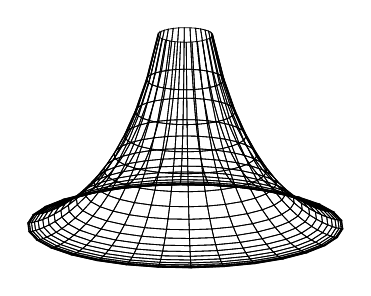
\begin{tikzpicture}[scale=0.75]
  \begin{axis}[view={20}{-20},hide axis]
  \def\d{1.};
  \addplot3[mesh,black,domain=0:360,domain y=90:170,samples=31,samples y=20]
    ({\d*cos(x)*sin(y)},{\d*sin(x)*sin(y)},{\d*cos(y)+\d*ln(tan(y/2)});
  \end{axis}
  \end{tikzpicture}
  \end{center}
  \caption{Portion of the upper half of a pseudosphere, a surface with constant
  negative curvature.}
\end{marginfigure}

One of the initial difficulties in grasping the intrinsic meaning of curvature derives
from the fact that most of our intuition comes from embedding the variety of
interest into a higher-dimensional space, e.g., a one-dimensional curve in the
two-dimensional Euclidean plane or a two-dimensional surface into the Euclidean
three-dimensional space. For instance we might be tempted to qualify the circle
or the surface of a cylinder as \emph{curved} objects (whatever that means), while
in fact we shall learn that there is no intrinsic curvature in one
dimension\sidenote{We shall see that 2 is the minimum dimension allowing for a non
trivial Riemann tensor.}, and the cylinder is perfectly flat surface---which should
not sound completely unreasonable when you think about the fact that it can be obtained
by folding a piece of paper with no deformation, and therefore the usual Euclidean
geometry must apply.

For a bi-dimensional surface embedded in a three dimensional space the notion of
Gaussian curvature provides a well defined recipe to characterize the curvature
in any given point: you take the vector that is normal to the surface in that
point and, among all the planes containing this vector (the so called normal planes)
you pick the two for which the curvature radii $R_1$ and $R_2$ of the intersection
between the planes and the original surface are minimum and maximum. The Gaussian
curvature is then given by
\begin{align}\label{eq:gaussian_curvature}
  k = \frac{1}{R_1 R_2},
\end{align}
which explains why the cylinder is flat: the radius of curvature in the plane containing
the axis of the cylinder is infinite. This is also consistent with the notion that
a 2-sphere has a constant positive curvature $k = \nicefrac{1}{R^2}$ and that a
saddle has a negative curvature in the central part, where the two curvature radii
have opposite sign. In any event, whatever geneal definition of curvature we may
come up with, it will need to conform to these basic behavior we have introduced
at an intuitive level.

We note, in passing, that even our cursory discussion allows for devising a prescription
for \emph{measuring} the local curvature on a arbitrarily small portion of a surface
without ever leaving the surface, or embedding it into a higher-dimensional space.
Take a 2-sphere of radius $R$ and imagine measuring the length $C$ of the circumference
of radius $r$ centered at the north pole---this is defined as the locus of the points
whose distance from the pole, \emph{measured along the surface of the sphere}, is
exactly $r$\todo{Add a drawing}. The difference between the length we would expect
in a flat space $2\pi r$ and the measured length is
\begin{align*}
  2\pi r - C = 2\pi r - 2\pi R \sin\theta,
\end{align*}
where $\theta = \nicefrac{r}{R}$ is the angle at the center of the 2-sphere subtended
by our circumference. As we make $r$ smaller and smaller we can expand the expression
in a Taylor series, and we get
\begin{align*}
  \lim_{r\rightarrow 0} (2\pi r - C) \approx
  2\pi \left( r - R\theta + R \frac{\theta^3}{6} \right) =
  \frac{\pi}{3} \frac{r^3}{R^2}
\end{align*}
which, in our language, we can rewrite as
\begin{align}
  K = \frac{1}{R^2} = \frac{3}{\pi} \lim_{r\rightarrow 0} \frac{2\pi r - C}{r^3}.
\end{align}
That is: we measure $r$ and $C$, and if it turns out that $C < 2\pi r$ ($C > 2\pi r$),
then we know we are in a point on our surface where the curvature is positive (negative).



\subsection{The metric connection}

One of the first problems that we encounter when we abandon flat spaces is that,
while the partial derivative of a scalar $\partial_\mu \phi$ remains a perfectly
legitimate four-vector, this nice property does not scale to more complex objects,
as can be seen in the simple case of the derivative of a vector $\partial_\nu V^\mu$:
\begin{align*}
  \partial_{\nu'} V^{\mu'} =
  \partial_{\nu'} \left( \pdv{x^{\mu'}}{x^\lambda} V^\lambda \right) =
  %\pdv{x^{\mu'}}{x^\lambda} \partial_{\nu'} V^\lambda +
  \overbrace{\pdv{x^{\mu'}}{x^\lambda} \pdv{x^{\rho}}{x^{\nu'}} \partial_{\rho} V^\lambda}^{\text{tensor}} +
  \overbrace{V^\lambda \partial_{\nu'} \left( \pdv{x^{\mu'}}{x^\lambda} \right)}^{\text{not a tensor}}.
\end{align*}
The first part does indeed transform like a tensor, but in the second term we have
the derivative of the transformation law, which we had not see, so far. That means
that $\partial_\nu V^\mu$, that we would love to be a legitimate $(1,~1)$ tensor,
in fact is not.

If we want to be able to express the law of Physics in a way that is independent
of the particular coordinate system (i.e., in covariant form) then we need to build
a \emph{covariant derivative} that reduces to the usual partial derivative on a
flat space but, when applied to an arbitrary tensor, still transforms as a tensor
on an arbitrary (flat or curved) space.
It is possible to demonstrate that, if we require this new operator to be linear
and satisfy the usual product rule (which sounds fairly reasonable)\sidenote{In fact
in order to be able to use the same linear transformation on both vectors and one-forms,
we shall also require that the Kronecker delta is covariantly constant
\begin{align*}
  \nabla_\mu \delta^\mu_\nu = 0
\end{align*}
and that it reduces to the partial derivative when applied to a scalar
\begin{align*}
  \nabla_\mu \phi = \partial_\mu \phi.
\end{align*}
With this prescription the covariant derivative for a one-form reads
\begin{align}
  \nabla_\mu \omega_\nu =
  \partial _\mu \omega_\nu - \christoffel{\lambda}{\mu\nu}\omega_\lambda
\end{align}
(note the minus sign and the different index matching). Covariant derivative for
arbitrary $(n,~m)$ tensors are constructed by summing the partial derivative with
$n + m$ additional terms, with the proper sign and index matching.
}, then it can always be written as the sum of the good old partial derivative
plus a linear transformation
\begin{align}
  \nabla_\mu V^\nu = \derx{\mu} V^\nu + \christoffel{\nu}{\mu\lambda}V^\lambda.
\end{align}

We call the new object $\christoffel{\nu}{\mu\lambda}$ a \emph{connection}. Let's
just state up front that the connection is not a tensor (which you might have guess
by the fact that we have been sloppy in placing the indices one on top of the other
without paying attention to the order); this should not come out as a surprise,
because if $\nabla_\mu V^\nu$ is a tensor and $\derx{\mu} V^\nu$ is not, whatever
is left on the right-hand side of the equation should not be a tensor either.
(In fact it is purposely constructed as the non-tensorial quantity that needs to
be added to the usual derivative to build an object does transform like a tensor.)
The name "connection" comes from the fact in order to take the derivative we need
to compare vectors (or tensors) in nearby points of the spacetime, or, in other
words, we need to be able to \emph{transport} vectors from one point to another,
and the connection does exactly this.

Now, this is all trivial in a flat space, where we can easily parallel-transport
stuff with no ambiguity, but is trickier in a curved space, where the result of a
parallel transport depends on the path followed, and there is just no unique prescription
to be followed\sidenote{This is actually far reaching, as it implies, for instance,
that in general relativity is impossible to define the notion of relative velocities
for two particles in two different points of a curved space or, for what matters,
two far-away galaxies in a curved universe.}. This is peraps most clear if you think
about a vector at a point of the equator of a 2-sphere pointing toward the pole
along a meridian---if you parallel-transport by 90 degrees in longitude and then
parallel-transport it to the pole, it will be orthogonal to the result of a simple
parallel transport to the pole of the original vector. As a consequence, in general
we can define multiple connections on any given manifold, and any of them will
provide a different covariant derivative.\todo{Add a drawing.}

At this point you might be unclear on whether the connection derives from the metric
or not---your initial guess might have been that it does, but then why can I have
many different connections on the same manifold? Well, the answer is no, and in
fact you don't even need a metric tensor to define a connection. The nice thing,
however, is  that if you do have a metric tensors $g_{\mu\nu}$ to start with, then
the latter uniquely identifies a connection if we require two additional properties
\begin{align*}
  \christoffel{\lambda}{\mu\nu} = \christoffel{\lambda}{\nu\mu} & \quad
  \text{(torsion free)}\\
  \nabla_\rho g_{\mu\nu} = 0 & \quad \text{(metric compatibility)}
\end{align*}
This particular connection is called \emph{metric compatible} and can be explicitly
written in terms of the metric as
\begin{align}
  \christoffel{\lambda}{\mu\nu} = \frac{1}{2}g^{\lambda\sigma}
  (\derx{\mu}g_{\nu\sigma} + \derx{\nu}g_{\sigma\mu} - \derx{\sigma}g_{\mu\nu}).
\end{align}
(Note that all the three indices in the three terms in parentheses move from the
right to the left, wrapping over at the beginning, and there is an extra minus sign
when the index we are contracting over ($\sigma$, in this case) is attached to the
derivative.) As far as we are concerned, this will be \emph{the} connection we shall
always use\sidenote{From a physical point of view, a metric-compatible connection
has the notable property of preserving the norm (and orthogonality) of the vectors.
Also, a metric-compatible covariant derivative commutes with the operation of raising
and lowering indices.}. Sometimes it is called the Christoffel connection, and its
coefficients the Christoffel symbols. We note that it is trivial to verify that the
Christoffel connection is symmetric in the two lower indices, owing to the fact
that the metric tensor is symmetric
\begin{align*}
  \christoffel{\lambda}{\nu\mu} = \frac{1}{2}g^{\lambda\sigma}
  (\derx{\nu}g_{\mu\sigma} + \derx{\mu}g_{\sigma\nu} - \derx{\sigma}g_{\nu\mu}) =
  \christoffel{\lambda}{\mu\nu}.
\end{align*}
Verifying that the Christoffel connection is metric compatible by direct calculation
is somewhat more tedious, but definitely doable.



\subsection{The Riemann tensor}

We now have all the basic ingredient that we need for a rigorous definition of the
curvature. If we go back to the example of the parallel transport on the 2-sphere
we have seen in the previous section, one of the ways that curvature manifested
itself in that case was the fact that \emph{a parallel transport over a closed loop
was not leaving the original vector unchanged}. This is a good hint, as one of the
possible ways we can characterize the curvature of a manifold at a specific point
is to calculate the change of a given vector $V^\sigma$ when parallel transported
across an infinitesimal loop around the point, e.g., a square defined by the (small)
vectors $A^\mu$ and $B^\nu$.

Without any proof, we shall limit ourselves to the answer: all the information about
the curvature of a manifold is embedded into the Riemann tensor (of the second
kind)\sidenote{Since the change $\delta V^\rho$ represents a linear transformation
on the vector $v^\sigma$, and also depends on the sides of the loop $A^\mu$ and
$B^\nu$ it makes sense that the thing has one upper index and three lower indices
to be contracted. We also expect the Riemann tensor to be antisymmetric in the last
two indices, since swapping the order of $A^\mu$ and $B^\nu$ corresponds to reversing
the direction in which the loop is traversed, which should give the opposite answer.}
\begin{align}\label{eq:riemann_tensor}
  \riemann{\rho}{\sigma\mu\nu} =
  \derx{\mu}\christoffel{\rho}{\nu\sigma} - \derx{\nu}\christoffel{\rho}{\mu\sigma} +
  \christoffel{\rho}{\mu\lambda}\christoffel{\lambda}{\nu\sigma} -
  \christoffel{\rho}{\nu\lambda}\christoffel{\lambda}{\mu\sigma}.
\end{align}

We do not dare to demonstrate that this transforms as a tensor, but it does: it is
constructed from non tensorial elements in a unique combination that has good
transformation properties. It is a pure function of the geometrical properties
of the space time (the connection and its derivatives). It is a function of the
point in space, and it vanishes if and only if the metric is flat anywhere.

The Riemann tensor has a number of symmetries reducing the number of independent
component from the original $n^4$ (in a $n$-dimensional space), and this symmetries
are most easily explored in the fully covariant form\sidenote{This is sometimes
referred to as the Riemann tensor of the first kind.} of the tensor itself
\begin{align*}
  \riemann{}{\rho\sigma\mu\nu} = g_{\rho\lambda}\riemann{\lambda}{\sigma\mu\nu}.
\end{align*}
It can be shown that this is antisymmetric in the first two indices and
invariant under the interchange of the first pair of indices with the second
\begin{align*}
  \riemann{}{\rho\sigma\mu\nu} = -\riemann{}{\sigma\rho\mu\nu}
  \quad \text{and} \quad
  \riemann{}{\rho\sigma\mu\nu} = \riemann{}{\mu\nu\rho\sigma};
\end{align*}
The antisymmetric property, in particular, is quite powerful, as it implies that
many of the components of the tensors are vanishing.
In addition, it can be shown that the sum of cyclic permutations of the last three
indices vanishes
\begin{align*}
  \riemann{}{\rho\sigma\mu\nu} + \riemann{}{\rho\mu\nu\sigma} + \riemann{}{\rho\nu\sigma\mu} = 0.
\end{align*}
All of this put together, it can be shown that in $n$ dimensions the Riemann tensor
has $n^2 (n^2 - 1) / 12$ independent components: that is $20$ in four~dimensions,
$6$ in three dimensions, and only $1$ in two dimensions. As we have already noted,
there is no intrinsic curvature in one dimension.

The contraction of the Riemann tensor is interesting, for reasons that we shall see
in a moment. If we contract a first time we get the Ricci tensor\sidenote{Note the
Ricci tensor assciated with the Christoffel connection is automatically symmetric.}
\begin{align}\label{eq:ricci_tensor}
  \ricci{\mu\nu} = \riemann{\lambda}{\mu\lambda\nu},
\end{align}
and by contracting a second time we get the Ricci scalar
\begin{align}\label{eq:ricci_scalar}
  \ricci{} = \mathcal{R}^\mu_{\phantom{\mu}\mu} = g^{\mu\nu} \ricci{\mu\nu}
\end{align}
which essentially encapsulates the curvature of the spacetime as a function of the
position.

Before we move on to the next section, where we shall see many of the concepts we
have introduced in actions, it is worth stating (without demonstration) the Bianchi
identity, that we write in the particular form\sidenote{If you are surprised seeing
a covariant derivative with an upper index, note it is the fact that we are using
a metric-compatible connection that allows to raise the index, here.}
\begin{align}\label{eq:bianchi_identity}
  \nabla^\mu \ricci{\rho\mu} = \frac{1}{2} \nabla_\rho \ricci{}.
\end{align}
This allows to define the Einstein tensor
\begin{align}
  G_{\mu\nu} = \ricci{\mu\nu} - \frac{1}{2} \ricci{} g_{\mu\nu},
\end{align}
that is divergenceless, in the sense\sidenote{Mind it is the fact we are using a
metric-compatible connection that ensures that the metric commutes with the
covariant derivative, and that the last term is identically zero.}
\begin{align*}
  \nabla^\mu G_{\mu\nu} =
  %\nabla^\mu \ricci{\mu\nu} - \frac{1}{2} \nabla^\mu \left( \ricci{}g_{\mu\nu} \right) =
  \frac{1}{2}\nabla_\nu \ricci{} - g_{\mu\nu} \nabla^\mu \ricci{} -
  \cancel{\frac{1}{2}\ricci{} \nabla^\mu g_{\mu\nu}} = 0.
\end{align*}



\subsection{A worked-out example}

The previous section, admittedly, is a pretty terse introduction to curvature.
Rather than going through all the gory details about why the various things we
have introduced are defined the way they are and behave the way they do, we shall
work out a concrete example of a simple (positively) curved surface---that of the
2-sphere, that is, the two-dimensional surface of a sphere of radius $R$ embedded
in three dimensions.

We shall work in polar coordinates, where $x^1 = \theta$ and $x^2 = \phi$ and, since
we are dealing with spatial indices only, we shall denote them with latin letters
instead of greek ones. The infinitesimal interval reads
\begin{align*}
  \dss = R^2 d\theta^2 + R^2 \sin^2\theta d\phi^2,
\end{align*}
which allows to write the metric tensor and its inverse in the form\sidenote{The
reader should note how upper and lower indices make a huge difference in the metric
tensor, which is not obviously the case in the old, good Minkowski spacetime.}
\begin{align*}
  g_{ij} =
  \begin{pmatrix}
    R^2 & 0\\
    0 & R^2 \sin^2 \theta \\
  \end{pmatrix}
  \quadtext{and}
  g^{ij} =
  \begin{pmatrix}
    \nicefrac{1}{R^2} & 0\\
    0 & \nicefrac{1}{R^2 \sin^2 \theta} \\
  \end{pmatrix}
\end{align*}
with the indices $i$ and $j$ running from $0$ to $1$.

Let us start from the connection. In principle we have $2^3 = 8$ Christoffel symbols,
but it is easy to convince ourselves that in our case most of them are zero, given
that the metric is diagonal
\begin{align*}
  g_{12} = g_{21} = 0
\end{align*}
and, among the derivatives, only $\derx{1}g_{22}$ survives, while all the others
are zero
\begin{align*}
  \derx{1}g_{11} = \derx{2}g_{11} = \derx{2}g_{22} = 0.
\end{align*}
As it turns out, the only non-trivial connections are
\begin{align*}
  \christoffel{1}{22} & =
  \frac{g^{11}}{2} (\derx{2}\cancel{g_{21}} + \derx{2}\cancel{g_{12}} - \derx{1}g_{22}) +
  \frac{g^{12}}{2} (\cancel{\derx{2}g_{22}} + \cancel{\derx{2}g_{22}} - \cancel{\derx{2}g_{22}}) =\\
  & = -\frac{g^{11}}{2} \derx{1}g_{22} =
  -\frac{1}{2R^2} \pdv{R^2 \sin^2 \theta}{\theta} = -\sin\theta \cos\theta\\
% \end{align*}
% and
% \begin{align*}
  \christoffel{2}{12} & =
  \frac{g^{21}}{2} (\derx{1}\cancel{g_{21}} + \cancel{\derx{2}g_{11}} - \derx{1}\cancel{g_{12}}) +
  \frac{g^{22}}{2} (\derx{1}g_{22} + \derx{2}\cancel{g_{21}} - \derx{2}\cancel{g_{12}}) =\\
  & = \frac{g^{22}}{2} \derx{1}g_{22} =
  \frac{1}{2R^2\sin^2\theta} \pdv{R^2 \sin^2 \theta}{\theta} = \frac{\cos\theta}{\sin\theta}
\end{align*}
(Since the Christoffel connection is torsion free, i.e., symmetric in the two lower
indices, $\christoffel{2}{12} = \christoffel{2}{21}$.)

Moving on, since we are in dimension~2, we know that the fully covariant Riemann
tensor has only one independent component different from zero, which we can take
to be $\riemann{}{1212}$, and all the other follows from the cyclic permutation
rules of the indices
\begin{align*}
  \riemann{}{1212} =
  g_{11} \riemann{1}{212} + \cancel{g_{12}} \riemann{2}{212} = g_{11} \riemann{1}{212},
\end{align*}
so that we are left with a single component of the Riemann tensor of the second kind to
calculate\sidenote{We note that $\riemann{1}{212} = -\riemann{1}{221}$.
Also, for completeness, the other non-trivial such Riemann tensor is
\begin{align*}
  \riemann{2}{121} = -\riemann{2}{112} = 1,
\end{align*}
which we don't calculate explicitly as it is not strictly necessary, here. (If you
are confused about the existence of two different components of the Riemann tensor
of the second kind, remember that the counting we did for the number of independent
components was for the version with all lower indices.)}:
\begin{align*}
  \riemann{1}{212} & =
  \derx{1}\christoffel{1}{22} - \derx{2} \cancel{\christoffel{1}{12}} +
  (\cancel{\christoffel{1}{11}}\christoffel{1}{22} +
    \cancel{\christoffel{1}{21}}\cancel{\christoffel{2}{22}}) -
  (\cancel{\christoffel{1}{12}}\cancel{\christoffel{1}{21}} +
    \christoffel{1}{22}\christoffel{2}{21}) =\\
  & = -\pdv{\sin\theta \cos\theta}{\theta} + \cos^2\theta =
  \sin^2 \theta.
\end{align*}
% and
% \begin{align*}
%   \riemann{2}{121} & =
%   \derx{2}\cancel{\christoffel{2}{11}} - \derx{1} \christoffel{2}{21} +
%   (\christoffel{2}{21} \cancel{\christoffel{1}{11}} +
%     \cancel{\christoffel{2}{22}}\cancel{\christoffel{2}{11}}) -
%   (\cancel{\christoffel{2}{11}}\cancel{\christoffel{1}{21}} +
%     \christoffel{2}{12}\christoffel{2}{21}) =\\
%   & = \pdv{\nicefrac{\cos\theta}{\sin\theta}}{\theta} - \frac{\cos^2\theta}{\sin^2\theta} = 1
%   \quad \left(= -\riemann{2}{112}\right)
% \end{align*}
It follows that the only non trivial component of the Riemann tensor of the
first kind is
\begin{align*}
  \riemann{}{1212} = \riemann{}{2112} = - \riemann{}{2121} = -\riemann{}{1212} = R^2\sin^2\theta.
\end{align*}

The contraction yielding the Ricci tensor, now that we have all the relevant components
of the Riemann tensors calculated, is trivial
\begin{align*}
  \begin{cases}
  \ricci{11} & = \cancel{\riemann{1}{111}} + \riemann{2}{121} = 1\\
  \ricci{22} & = \riemann{1}{212} + \cancel{\riemann{2}{222}} = \sin^2\theta
  \end{cases}\quad\text{or}\quad
  \ricci{ij} =
  \begin{pmatrix}
    1 & 0\\
    0 & \sin^2\theta\\
  \end{pmatrix} = \frac{1}{R^2} g_{ij}
\end{align*}
and we can close the loop calculating the trace of the Ricci tensor, yielding the
Ricci scalar\sidenote{On a 2-dimensional surface the Ricci scalar is just twice the
Gaussian curvature
\begin{align*}
  \ricci{} = 2K,
\end{align*}
as we have calculated explicitly in this case.
}
\begin{align*}
  \ricci{} = g^{ij} \ricci{ij} = \frac{1}{R^2} g^{ij} g_{ij} =
  \frac{1}{R^2} \delta^i_i = \frac{2}{R^2}.
\end{align*}

Wow---this was quite a journey! But at least now you should get a sense of how things
work, and appreciate the fact that, in more elaborated examples, things tend to get out
of hand quite quickly. (Also, you should be happy to know that we will not be spending
much time calculating Christoffel symbols and alike, in the following of these notes.)



\subsection{More fun with curvature}

A couple more things about the notion of curvature on simple two-dimensional manifolds
before we move on. If we repeat the same exact process we went through for the
2-sphere in the case of a cylinder of radius $R$, using cylindrical coordinates
$x^1 = z$ and $x^2 = \phi$, the metric tensor reads
\begin{align*}
  \dss = dz^2 + R^2 d\phi^2 \quadtext{or}
  g_{ij} =
  \begin{pmatrix}
    1 & 0\\
    0 & R^2\\
  \end{pmatrix}
\end{align*}
we immediately realize that \emph{all} the derivatives of the metric vanish, and
so do all the Christoffel symbols, along with the components of the Riemann and
Ricci tensor. As a consequence the Ricci scalar is zero---the 2-dimensional surface
of a cylinder embedded in the 3-dimensional space, as we said at the beginning of
this section, is flat.

Incidentally, the metric tensor for the cylinder is very similar to that associated
with a flat bi-dimensional space where we choose a polar coordinate system
$x^1 = r$ and $x^2 = \phi$:
\begin{align*}
  \dss = dr^2 + r^2 d\phi^2 \quadtext{or}
  g_{ij} =
  \begin{pmatrix}
    1 & 0\\
    0 & r^2\\
  \end{pmatrix}
\end{align*}
but the seemingly small difference ($r$ vs. $R$) has important consequences because,
while $R$ in the case of the cylinder was a constant, $r$ here is one of the
coordinates---now the metric depends explicitly on the position, and the Christoffel
symbols do not vanish anymore. We will not go through the full calculation again,
but the non-trivial components of the Christoffel connection read
\begin{align*}
  \christoffel{1}{22} = -r \quadtext{and}
  \christoffel{2}{12} = \christoffel{2}{21} = \frac{1}{r}.
\end{align*}
The big difference is that now the only non-trivial component of the Riemann tensor,
that we can calculate exactly like before, reads
\begin{align*}
  \riemann{1}{212} & =
  \derx{1}\christoffel{1}{22} - \derx{2} \cancel{\christoffel{1}{12}} +
  (\cancel{\christoffel{1}{11}}\christoffel{1}{22} +
    \cancel{\christoffel{1}{21}}\cancel{\christoffel{2}{22}}) -
  (\cancel{\christoffel{1}{12}}\cancel{\christoffel{1}{21}} +
    \christoffel{1}{22}\christoffel{2}{21}) =\\
  & = -\pdv{r}{r} - \left( -r \cdot \frac{1}{r} \right) = -1 + 1 = 0,
\end{align*}
i.e., it vanishes identically. This is a nice illustration of how the metric tensor
does not have to be trivial, even in flat space, provided that the coordinate system
is extravagant enough. And yet polar coordinates on the plane describe the same
old flat space, just as cartesian coordinates do.



\section{The energy-momentum tensor}

Now that we know how to handle geometry in a curved spacetime, we turn our eyes to
the fundamental question: what is the origin of the deformation of the spacetime?
As it turns out, the answer to this question requires the introduction of the
energy-momentum tensor, which is also referred to in the literature as the stress-energy
tensor, and represents, the density and flux of energy and momentum---more specifically
$T^{\mu\nu}$ is the flux of four-momentum $p^\mu$ across a surface at constant $x^\nu$.
The stress-energy tensor does apply to matter, radiation and any non-gravitational\sidenote{In
general relativity gravitation does not count as a force, and expressing its energy
content in a local formulation is far from trivial} force field, but in fact we shall
be dealing uniquely with \emph{perfect fluids}\sidenote{We will not dig too much
into this, but a perfect fluid can be defined as one with no heat conduction and no
viscosity or, equivalently, one that looks isotropic in its rest frame. From a practical
standpoint, a perfect fluid is fully characterized by its density and pressure.}---as
we shall see, the universe itself can be modeled as a perfect fluid, albeit one with
multiple components.

Although the actual expression for the stress-energy tensor can be dauntingly complicated,
there are general things that can be said. In general relativity the stress-energy
tensor is symmetric. $T^{00}$ is the energy density in the co-moving reference
frame---for a perfect fluid it is just the energy density per unit volume $\edensity$.
The $T^{i0}$ components describe the energy flux while the $T^{0i}$ components represent
the density of momentum, and the two sets are identical owing to the symmetric nature
of the tensor. The spatial components $T^{ij}$ represent the stress, with the three
on the diagonal generally referred as pressure and those out of the diagonal as sheer stress.

For an infinitesimal element of a perfect fluid in its rest frame, where there is
no bulk motion, there is no energy flux and no sheer stress, and the three diagonal
space components $T^{ii}$ are all identical and represent the pressure of the fluid.
In special relativity the energy-momentum tensor takes the particularly simple
form\sidenote{Pay particular attention here, as in many books the energy density is
indicated as $\density$, which we use to indicate the mass density instead. To make
things more complicated, for a non relativistic fluid $\edensity = \density c^2$,
so in that case the energy density would be the mass density, modulo a constant
$c^2$, which is omitted when working in natural units.}
\begin{align}\label{eq:energy_momentum_tensor_sr_rest}
  T^{\mu\nu} =
  \begin{pmatrix}
    \edensity & 0 & 0 & 0\\
    0 & \pressure & 0 & 0\\
    0 & 0 & \pressure & 0\\
    0 & 0 & 0 & \pressure \\
  \end{pmatrix},
\end{align}
The stress-energy tensor naturally encapsulates the energy and momentum conservation
in the fact that, in absence of external forces, it is divergenceless\sidenote{Keep
in mind we are still in special relativity, so this is a perfectly legitimate tensorial
equation.}
\begin{align}
  \partial_\mu T^{\mu\nu} = 0,
\end{align}
which in this particular case reduces to the (admittedly, not very interesting)
conditions
\begin{align*}
  \pdv{\edensity}{t} = 0 \quad\text{and}\quad
  \grad{\pressure} = 0.
\end{align*}
That is, if fluid is at rest, for any particular point in space the time derivative
of the energy density (which in the non-relativistic case is proportional to the
mass density) is zero, and so is the spatial gradient of the pressure. No surprise,
everything is constant.

As it turns out, generalizing the formula for an arbitrary quadrivelocity $\velocity^\mu$
of the fluid element is rather easy, at least in special relativity, and the expression
we end up with is
\begin{align}\label{eq:stress_energy_sr}
  T^{\mu\nu} =
  \left(\edensity + \pressure \right) \frac{\velocity^\mu \velocity^\nu}{c^2} +
  \pressure \eta^{\mu\nu} \quad\text{(special relativity)}.
\end{align}
You can easily check for yourself that it reduces to the previous expression in the
rest frame of the fluid, where $\velocity^\mu = (c,~0,~0,~0)$, and since~\eqref{eq:stress_energy_sr}
is a perfectly good tensorial expression that provides the right answer in one
reference frame, then it is bound to be correct in all frames\sidenote{We will not
write down the detailed calculation, but it is not too difficult to show that in
the non-relativistic limit the energy-momentum conservation
\begin{align*}
  \derx{\mu}T^{\mu\nu},
\end{align*}
when projected along the four-velocity and orthogonally to it, yields the continuity
equation for the energy density and the non-relativistic Euler equation we have
derived in appendix~\ref{chap:fluidodynamics}.
}

We shall now take what is sometimes called the \emph{minimal-coupling principle} and
say that, since we have a law that is valid in every inertial frame in flat spacetime
and is written in tensorial form, we shall go ahead, change the Minkowski metric
$\eta^{\mu\nu}$ into the general metric $g^{\mu\nu}$
\begin{align}
  T^{\mu\nu} = \left(\edensity + \pressure \right) \frac{\velocity^\mu \velocity^\nu}{c^2} +
  \pressure g^{\mu\nu} \quad\text{(general relativity)},
\end{align}
change the ordinary derivative $\derx{\mu}$ with the covariant derivative $\nabla_\mu$,
and just assume that the conservation of energy and momentum can be written in general as
\begin{align}
  \nabla_\mu T^{\mu\nu} =
  \derx{\mu} T^{\mu\nu} + \christoffel{\mu}{\mu\lambda} T^{\lambda\nu} +
  \christoffel{\nu}{\mu\lambda} T^{\mu\lambda} = 0.
\end{align}
Let's commit this to memory, as this will be one of the two key ingredients for the
Einstein field equation.

And one more thing: we will not be needing this speficically for another few pages
but we take this chance to note that the trace of the energy-momentum tensor for
a perfect fluid in the reference system where the fluid is at rest is\sidenote{Make
sure you do not get confused with what the \emph{trace} of tensor really means:
you have to make sure you have one upper index and one lower index before treat it
like a matrix and sum up the diagonal terms. In general relativity the stress-energy
tensor in the rest frame reads
\begin{align*}
  T^{\mu\nu} =
  \begin{pmatrix}
    \edensity & 0 & 0 & 0\\
    0 & & & \\
    0 & & g^{ij}\pressure & \\
    0 & & & \\
  \end{pmatrix}.
\end{align*}
and if we lower an index, this transforms into a simpler, diagonal form
\begin{align*}
  T^{\mu}_{\phantom{\mu}\nu} = g_{\sigma\nu} T^{\mu\sigma} =
  \begin{pmatrix}
    -\edensity & 0 & 0 & 0\\
    0 & \pressure & 0 & 0\\
    0 & 0 & \pressure & 0\\
    0 & 0 & 0 & \pressure\\
  \end{pmatrix}
\end{align*}
by virtue of the contraction of the spatial part of the metric with its inverse.
Finally
\begin{align*}
  T = T^{\mu}_{\phantom{\mu}\mu} = -\edensity + 3\pressure.
\end{align*}
}
\begin{align}\label{eq:energy_momentum_tensor_trace}
  T = -\edensity + 3\pressure.
\end{align}



\subsection{Energy density, pressure and the equation of state}

At this point in the narration it is customary to face a first discussion on the
equation of state. The stress-energy tensor is constructed starting from the energy
density and the pressure of the fluid, but in fact the two quantities are in general
not independent, and we call any function linking the two an equation of state.
The relevance to our discussion should be immediately obvious, as if we can write,
say, the pressure as a function of the energy density, then all of a sudden we
have one less quantity in the mix.

This is hardly new, as in appendix~\ref{chap:qstat} we have already derived from
the first principles (the Bose-Einstein and Fermi-Dirac distributions) the equation
of state for a non-relativistic and an ultra-relativistic gas:
\begin{align*}
  \pressure =
  \begin{cases}
    \frac{2}{3}u \quad\text{non-relativistic}\\[10pt]
    \frac{1}{3}u \quad\text{ultra-relativistic}.
  \end{cases}
\end{align*}
There is, however, an important point that can hardly be stressed enough: while
the internal energy of a gas in the usual thermodynamic sense is intended as the
average of the \emph{kinetic energy} over the relevant distribution\sidenote{It is
no coincidence that we call $u$ the energy density in the context of
appendix~\ref{chap:qstat} while we call it $\edensity$ here.}, it is the
\emph{total energy}\sidenote{This is actually profound and far reaching, as it
implies that general relativity is sensitive to the absolute energy, and not to
just differences in energies, as most other theories. We shall come back to this
later, when discussing the cosmological constant.}, including the contribution from
the rest mass, that matters here
\begin{align*}
 E = \sqrt{p^2 c^2 + m^2 c^4} \rightarrow
 \begin{cases}
   mc^2 \quad & \text{(non-relativistic)}\\
   pc \quad & \text{(ultra-relativistic)}.
 \end{cases}
\end{align*}
It should be obvious that things are rigorously unchanged in the ultra-relativistic
case---total energy, kinetic energy (and momentum, for what matters, modulo a constant
$c$) are all the same thing anyway, and it is still true that
\begin{align}
  \pressure = \frac{1}{3} \edensity \quad \text{(ultra-relativistic, or radiation)}.
\end{align}
But in the non-relativistic limit, where $E \approx mc^2 \gg pc,~E_k,~\kT$ the story
is completely different, as
\begin{align*}
  \edensity = mc^2 n = \density c^2
  \quad \text{and} \quad
  \pressure = \frac{2}{3} \ave{E_k} n = \frac{1}{2} \density \ave{\velocity^2}.
\end{align*}
Since the average kinetic energy is much smaller than the rest mass, it follows that
$\pressure \ll \edensity$, and so much so that it can be taken to be zero
\begin{align}
  \pressure \approx 0 \quad \text{(non-relativistic, or matter)}.
\end{align}
Cosmologically speaking \emph{non-relativistic matter is pressureless} for all
practical purposes\sidenote{One simple way to convince yourself is to take air at
standard pressure (1~atm) and calculate the energy density implied by the rest mass
of the molecules. With a density $\density = 1.225$~kg~m$^{-3}$ the latter amounts
to
\begin{align*}
  \density c^2 \approx 10^{17}~\text{Pa} \approx 10^{12}~\text{atm}.
\end{align*}}.

As we shall see in the next section, these are not the only possibilities and,
mildly relativistic particles aside, there is at least another situation that will
be very important.



\section{The Einstein equation}\label{sec:efe}

We now have the basic ingredients to write the fundamental equations of dynamics
in general relativity. Let's go back for a second to the starting point of our original
program---we wanted to write the equivalent of the Netwtonian Poisson equation in the
form
\begin{align*}
  \text{curvature} = \text{mass-energy},
\end{align*}
and now we are fully equipped to do so in a tensorial fashion. On the right-hand
side we know that "mass-energy", in our language, means the energy momentum tensor
$T_{\mu\nu}$\sidenote{You might have noticed that we are using lower indices, here,
which is the opposite of what we did in the prvious section. We anticipate that
this is how the Einstein field equation is typically formulated because by doing this
we get the metric $g_{\mu\nu}$ (and not the inverse metric) on the other side of
the equal sign, but in fact we might have equivalently used upper indices.}.
One the left-hand side we need a $(0,~2)$ tensor that encapsulates the curvature of
the spacetime---at this point you will be jumping on the chair screaming that the
Ricci tensor $\ricci{\mu\nu}$ is just that! (We also note, in passing, that the
Ricci tensor is constructed with the second derivatives of the metric, which gives
us hope that it might reduce to the laplacian of the gravitational potential
$\nabla^2\Phi$ in the non relativistic limit.) If we were tempted to write\todo{Change
$k$ not to confuse it with the curvature.}
\begin{align*}
  \ricci{\mu\nu} = k T_{\mu\nu} \quad\text{(wrong!)}
\end{align*}
we would in fact be wrong, for the simple reason that, while the energy-momentum
tensor is divergenceless, the Ricci tensor is not\sidenote{If we really want to insist
on this field equation, by contracting with the metric we have
\begin{align*}
  \ricci{} = kT
\end{align*}
which, taken in conjunction with the Bianchi identity implies
\begin{align*}
  \nabla_v T = \derx{\nu} T = 0,
\end{align*}
i.e., the energy momentum tensor would be bound to be constant across the entire
spacetime, which makes no sense, as it is identically zero in vacuum and different
from zero in matter.}, and in fact the Bianchi identity~\eqref{eq:bianchi_identity}
tells us exactly what the divergence is
\begin{align*}
  \nabla^\mu T_{\mu\nu} = 0 \quad\text{but}\quad
  \nabla^\mu\ricci{\mu\nu} = \frac{1}{2}\nabla_\nu \ricci{} \neq 0.
\end{align*}

Of course this is resembling of a discussion that we have already had when we introduced
the Bianchi identity. We know already a $(0,~2)$ tensor that is constructed from
the Ricci tensor and is divergenceless---the Einstein tensor $G_{\mu\nu}$. We shall
therefore tentatively postulate that our field equation reads\sidenote{This is not,
in fact, the most general form of the field equation that we can devise with the
ingredients we have on the table. In particular, given the fact that we are using
a metric-compatible connection, we might as well add another term proportional to
the metric
\begin{align*}
  \ricci{\mu\nu} - \frac{1}{2}\ricci{}g_{\mu\nu} + \Lambda g_{\mu\nu}= kT_{\mu\nu}
\end{align*}
and everything would continue working as advertised. We shall refrain from elaborating
more on this topic right now, but we anticipate it will be important in the following.}
\begin{align*}
  \ricci{\mu\nu} - \frac{1}{2}\ricci{}g_{\mu\nu} = kT_{\mu\nu}
  \quad\text{(correct)}.
\end{align*}
The only piece of the puzzle that we are missing, here, is the constant of proportionality
$k$, but in order to gauge that we need to re-examine something that we have glanced
through, but not analyzed in detail---the geodesic equation.



\subsection{The geodesic equation and the Newtonian limit}

We have already said that in general relativity unaccelerated is synonym of free-falling,
and that a free-falling body follows a geodesic in a curved spacetime, but we have
never actually gone into the trouble of deriving the geodesic equation\sidenote{In
particular when we discussed the connection we took the stance that the latter is
defined in conjunction with the covariant derivative, simply because we have used
(and will use) the covariant derivative a lot, while in cosmology we are not so
much concerned with the motion of a test particle in curved spacetime.}, and it is
now time to make amend for this oversight.

In flat space an unaccelerated particle moves in straight lines, according to the
equation of motion
\begin{align}
   \dv[2]{x^\mu}{\tau} = 0,
\end{align}
where $\tau$ is the proper time\sidenote{As it turns out, at this stage we could
use any affine parameter $\lambda$ to parametrize our path $x^\mu(\lambda)$, but
since we will eventually fall back to the proper time, we might as well start with
that.}, that is, the time elapsed seen by an observer moving on a straight path
between two events ($\gamma d\tau = dt$).

Now, this is a second derivative of a vector, which does not transform as a vector,
and in order to write the corresponding equation of motion in general relativity,
we have to write it in covariant form. We can use the chain rule to get
\begin{align*}
  \dv{}{\tau} \left( \dv{x^\mu}{\tau} \right) =
  \dv{x^\nu}{\tau} \dv{}{x^\nu} \left( \dv{x^\mu}{\tau} \right) =
  \dv{x^\nu}{\tau} \partial_\nu \left( \dv{x^\mu}{\tau} \right) = 0.
\end{align*}
Now this is a good equation in tensorial form, and we can use again the minimal
coupling principle to generalize it to curved space---we just replace the partial
derivative with the covariant derivative
\begin{align*}
  \dv{x^\nu}{\tau} \partial_\nu \left( \dv{x^\mu}{\tau} \right) \rightarrow
  \dv{x^\nu}{\tau} \nabla_\nu \left( \dv{x^\mu}{\tau} \right) =
  \dv[2]{x^\mu}{\tau} + \christoffel{\mu}{\rho\sigma}\dv{x^\rho}{\tau}\dv{x^\sigma}{\tau}
\end{align*}
which yields the geodesic equation in its full glory
\begin{align*}
  \dv[2]{x^\mu}{\tau} + \christoffel{\mu}{\rho\sigma}\dv{x^\rho}{\tau}\dv{x^\sigma}{\tau} = 0
  \quad\text{(geodesic equation)}.
\end{align*}

It is instructive to see what happens in the Newtonian limit---hopefully we shall
recover everything that we know from classical mechanics. In order to do so we shall
require three distinct conditions to hold, namely
\begin{align*}
  \dv{x^i}{\tau} \ll \dv{x^0}{\tau} & \quad\text{(small velocity)}\\[8pt]
  \derx{0}g_{\mu\nu} = 0 & \quad\text{(static field)}\\[8pt]
  g_{\mu\nu} = \eta_{\mu\nu} + h_{\mu\nu}, \quad \abs{h_{\mu\nu}} \ll 1 & \quad\text{(weak field)}.
\end{align*}
The first one implies that all the terms in the geodesic equation corresponding
to lower spatial indices of the connection are negligible
\begin{align*}
  \dv[2]{x^\mu}{\tau} + \christoffel{\mu}{00}\left( \dv{x^0}{\tau} \right)^2 = 0,
\end{align*}
and the four remaining Christoffel symbols simplify considerably owing to the fact
that the field is static
\begin{align*}
  \christoffel{\mu}{00} =
  \frac{1}{2}g^{\mu\lambda} (\cancel{\derx{0}g_{\lambda 0}} + \cancel{\derx{0}g_{0\lambda}} -
  \derx{\lambda}g_{00}) =
  -\frac{1}{2}g^{\mu\lambda}\derx{\lambda}g_{00},
\end{align*}
which, to the first order in $h_{\mu\nu}$, further reduces to
\begin{align*}
  \christoffel{\mu}{00} \approx -\frac{1}{2}\eta^{\mu\lambda}\derx{\lambda}h_{00}.
\end{align*}
If we put everything together, the spacelike components of the geodesic equation
in the Newtonian limit read
\begin{align*}
  \dv[2]{x^i}{\tau} - \frac{1}{2} \derx{i}h_{00} \left( \dv{x^0}{\tau} \right)^2 = 0
  \quad\text{or}\quad
  \dv[2]{x^i}{t} = \frac{1}{2} c^2 \derx{i} h_{00}.
\end{align*}
But this is exactly the Newtonian equation of motion for a particle in a gravitational
potential $\Phi$, provided that we identify
\begin{align}
  h_{00} = -\frac{2\Phi}{c^2} \quad\text{and}\quad g_{00} =
  -\left(1 +  \frac{2\Phi}{c^2}\right).
\end{align}



\subsection{The field equation, at last}

We are finally ready to calculate the constant $k$ in the Einstein tentative field
equation
\begin{align*}
  \ricci{\mu\nu} - \frac{1}{2}\ricci{}g_{\mu\nu} = kT_{\mu\nu}
\end{align*}
by requiring that the latter reduces to the proper Poisson equation in the Newtonian
limit. If we contract both hands with the metric tensor
\begin{align*}
  \overbrace{g^{\mu\nu}\ricci{\mu\nu}}^{\ricci{}} -
  \frac{1}{2}\ricci{} \overbrace{g^{\mu\nu}g_{\mu\nu}}^{4} = k \overbrace{g^{\mu\nu}T_{\mu\nu}}^{T}
  \quad \text{or}\quad \ricci{} = -kT
\end{align*}
we can rewrite it in the equivalent formulation, which is handy for our purposes
\begin{align*}
  \ricci{\mu\nu} = k\left( T_{\mu\nu} - \frac{1}{2}Tg_{\mu\nu} \right).
\end{align*}

Let us now consider a massive body in its rest frame, which in our language is a
pressureless fluid, where the only non-vanishing element of the energy-momentum
tensor is the energy density
\begin{align*}
  T_{00} = \density c^2 \quad\text{and}\quad T = g^{00}T_{00} = -\density c^2.
\end{align*}
The $00$ component of our field equation becomes then
\begin{align*}
  \ricci{00} = \nicefrac{1}{2}k\density c^2,
\end{align*}
and the only thing left to calculate is\sidenote{Remember that we have already
calculated all the Christoffel symbols in the Newtonian limit. To first order they
are linear in $h$ and therefore we can neglect the product of two symbols, since
the result is quadratic in $h$. In addition, we know that
\begin{align*}
  \christoffel{\mu}{00} \approx -\frac{1}{2}\eta^{\mu\lambda}\derx{\lambda}h_{00},
\end{align*}
from which it follows that the spacelike components read
\begin{align*}
  \christoffel{i}{00} \approx -\frac{1}{2}\eta^{i\lambda}\derx{\lambda}h_{00}.
\end{align*}
The sum over $\lambda$, here, formally runs over $0\dots 3$, but the first term
can be omitted because $\derx{0}h_{00} = 0$, and therefore
\begin{align*}
  \christoffel{i}{00} \approx -\frac{1}{2}\eta^{ij}\derx{j}h_{00} =
  -\frac{1}{2} \derx{i} h_{00}.
\end{align*}
(Keep in mind the spatial part of the Minkowski metric is the identity $I_{3\times 3}$.)}
\begin{align*}
  \ricci{00} & = \riemann{i}{0i0} =
  \derx{i}\christoffel{i}{00} -
  \overbrace{\cancel{\derx{0}\christoffel{i}{i0}}}^\text{static} +
  \overbrace{\christoffel{i}{i\lambda}\christoffel{\lambda}{00} -
  \christoffel{i}{0\lambda}\christoffel{\lambda}{i0}}^\text{second order}
  \approx \derx{i}\christoffel{i}{00} = -\frac{1}{2} \nabla^2 h_{00}.
  %& = -\frac{1}{2} \delta^{ij}\derx{i}\derx{j}h_{00} = -\frac{1}{2} \nabla^2 h_{00} =
  %\frac{1}{c^2} \nabla^2 \Phi.
\end{align*}
But we have already calculated how $h_{00}$ relates to the gravitational potential
$\Phi$, and it is trivial to verify that our tentative field equation reduces to
the Poisson equation in the Newtonian limit if $k = \nicefrac{8\pi G}{c^4}$---and
therefore we end up with
\begin{align}\label{eq:einstain_equation}
  \ricci{\mu\nu} - \frac{1}{2}\ricci{}g_{\mu\nu} = \frac{8\pi G}{c^4} T_{\mu\nu}
  \quad\text{(Einstein field equation)}.
\end{align}
We shall commit to memory the equivalent formulation we have worked out earlier
in this section
\begin{align}\label{eq:einstain_equation_alt}
  \ricci{\mu\nu} = \frac{8\pi G}{c^4} \left( T_{\mu\nu} -\frac{1}{2} T g_{\mu\nu} \right)
\end{align}
because it makes immediately obvious that in vacuum, where the energy-momentum
vanishes, the Einstein equation is simply
\begin{align}
  \ricci{\mu\nu} = 0.
\end{align}


\subsection{The cosmological constant}

We have already stated earlier in a note that~\eqref{eq:einstain_equation} is not
the more general field equation we can write with the ingredients in our toolbox.
Particularly, since when using the Christoffel (i.e., metric compatible) connection
the covariant derivative of the metric vanished identically, we have another
divergenceless $(0, 2)$ tensor (the metric itself) that we can throw in the mix, and
\begin{align}
  \ricci{\mu\nu} - \frac{1}{2} \ricci{} g_{\mu\nu} + \Lambda g_{\mu\nu} =
  \frac{8\pi G}{c^4} T_{\mu\nu}
\end{align}
is just as good as~\eqref{eq:einstain_equation} as a field equation\sidenote{At this
point you might start asking yourself how many more pieces (and which) we left out
but in fact, under very reasonable assumptions, this is actually the most general field
equation that we can write in four dimensions---a result that is known as the Lovelock
theorem.}. The constant $\Lambda$ usually goes under the name of  \emph{cosmological constant},
and its story is interesting: it was added by Einstein after the fact in the hope
of being able to produce a static universe, then retracted a few years later as a
terrible mistake, and finally established in the 1990s as an experimental evidence.

We shall come back to the cosmological constant in due time, after we have established
the basic equation ruling the evolution of the universe, but since we are at it,
it is worth noting that, if we rewrite the Einstein equation (with the cosmological
constant) in the form
\begin{align}
  \ricci{}^{\mu\nu} - \frac{1}{2} \ricci{} g^{\mu\nu} =
  \frac{8\pi G}{c^4} \left( T^{\mu\nu} - \frac{\Lambda c^4}{8\pi G} g^{\mu\nu} \right)
\end{align}
we can sweep it under the rug and pretend the cosmological constant did not exists,
modulo writing a new energy-momentum tensor that includes a \emph{vacuum density}
\begin{align}
  \edensity_\Lambda = \frac{\Lambda c^4}{8\pi G} \quad\text{(vacuum energy)}.
\end{align}
This is related to the fact that, as we noted earlier, the source term in general
relativity corresponds to the entire energy momentum tensor, and if the vacuum has
a non-zero constant energy, this will have measurable implications, as opposed to
what happens in all the theories that we know, where what matter are really differences
in energies. We shall use "cosmological constant" and "vacuum energy" as synonyms.
The latter is widespread in the literature, but the former reminds us that, in a
proper field theory, the vacuum energy is something that ought to be calculable, and
not a mere external parameter.

That all said, it is instructive to write the explicit expression for the new
energy-momentum tensor assuming a Minkowski-like metric, in the system where the
vacuum is at rest (whatever that means), so that we  can compare it directly
with~\eqref{eq:energy_momentum_tensor_sr_rest}:
\begin{align*}
  T^{\mu\nu} \rightarrow
  T^{\mu\nu} - \edensity_\Lambda \eta^{\mu\nu} =
  \begin{pmatrix}
    \edensity + \edensity_\Lambda & 0 & 0 & 0\\
    0 & \pressure - \edensity_\Lambda & 0 & 0\\
    0 & 0 & \pressure - \edensity_\Lambda & 0\\
    0 & 0 & 0 & \pressure - \edensity_\Lambda \\
  \end{pmatrix}.
\end{align*}
Now, the component of this new energy-momentum tensor corresponding to the vacuum
energy has the peculiar equation of state
\begin{align}
  \pressure = -\edensity,
\end{align}
which we add to our menu for the equation of states, along with that for (non-relativistic)
matter and that for (ultra-relativistic) radiation.



\section{The cosmological principle revisited}

We are already familiar with the cosmological principle, stating that the universe
is isotropic and homogeneous on large scales. Without entering into a philosophical
debate, what we actually measure is the isotropy of the universe, as seen from the
Earth: this is testified by the distribution of distant galaxies, the observation of the
X- and $\gamma$-ray backgrounds and, above all, the isotropy of the CMB. If, in
addition to that, we accept that the Earth occupies no special place in the universe
(which we called the Copernican principle) we are forced to accept that the universe
is isotropic when seen from any point, and therefore is homogeneous, too.

It is important to emphasize all of this applies to the space part of the spacetime.
We are also familiar that the our na\"ive understanding of the redshift is compatible
with a uniform expansion of the universe, and therefore we shall postulate that latter
is \emph{spatially} homogeneous and isotropic, but evolving in time\sidenote{There
also exists a \emph{perfect cosmological principle}, postulating that not only there
are no privileged locations in space, but there are no privileged moments in time.
It can be demonstrated that in a maximally symmetric $n$-dimensional spacetime
\begin{align*}
  \riemann{}{\rho\sigma\mu\nu} =
  \frac{R (g_{\rho\mu}g_{\sigma_\nu} - g_{\rho\nu}g_{\sigma_\mu})}{n(n - 1)},
\end{align*}
and the Einstein equation implies that the energy-momentum tensor is proportional
to the metric---all there is space for is cosmological constant, with no matter
and no radiation. No wonder this went of fashion when, after the discovery of the
CMB, the debate between the steady-state and the big-bang theory was settled in
favor of the latter.}.

Now, if we want to describe the universe as a homogeneous perfect fluid undergoing an
isotropic expansion, the first thing that we need to understand is which kind of
general metric tensor might describe just that.



\subsection{The FLRW metric}

The problem of the most general metric tensor compatible with our statement of the
cosmological principle was solved by Robertson and Walker in the 1930s, but since
some of the implications had already been previously explored by Alexander Friedman
and George Lemaitre, the metric is called the Friedman-Lemaitre-Robertson-Walker
(FLRW) metric. The basic idea is that we are looking for a factorization of our spacetime
in the form $\mathbf{R} \times \Sigma$, where $\mathbf{R}$ represents the time-like
coordinate, and $\Sigma$ is a maximally symmetric three-dimensional manifold, with
a time-dependent scale factor or
\begin{align*}
  \dss = -c^2dt^2 + a^2(t) d\sigma^2.
\end{align*}
Note we are implicitly working in \emph{co-moving coordinates}, i.e., a coordinate
system where an observer at rest perceives the universe as isotropic and the co-moving
distance $\chi_{12}$ between two object embedded in the Hubble flow remains
constant \sidenote{The Earth is not comoving, as the Solar system has a peculiar
velocity of about 370~km~s$^{-1}$ with respect to the cosmic rest frame, causing
a dipole signature in the observed angular distribution of the CMB temperature,
which needs to be subtracted in order to gauge the actual cosmological temperature
fluctuations.}, while the change in their physical distance is only encoded in the
scale factor $a(t)$.

In order to gauge how the spatial part $d\sigma^2$ of the interval might look like
we note that, although at this point we are completely agnostic about the curvature
(e.g., whether it should be positive, negative or zero) the homogeneity implies
that it will be constant everywhere over our manifold. In addition, the fact that
the universe  is isotropic suggests that we use spherical coordinates for the angular
part of the interval, and in fact we know exactly how the spatial part of the interval
should look like in a flat space
\begin{align}\label{eq:spherical_line_element_flat}
  d\sigma^2 = dr^2 + r^2 (d\theta^2 + \sin^2\theta d\phi^2).
\end{align}

Now, one way to generalize this to a (uniformly) curved space is to start from
a simple case. The 3-sphere $S^3$ would be the obvious thing to look at for the case
of a surface with positive uniform curvature, but since that is not trivial to visualize,
we shall move down in dimension $2$, instead, and see what it takes to generalize
the familiar interval in a flat space described in polar coordinates
\begin{align}\label{eq:polar_line_element_flat}
  d\sigma^2 = dr^2 + r^2 d\phi^2
\end{align}
to the 2-sphere $S^2$ of radius $R$. The line element in this case reads
\begin{align*}
  d\sigma^2 = R^2 d\theta^2 + R^2 \sin^2\theta d\phi^2,
\end{align*}
and we want to express, as before, it in terms of $(r,~\phi)$, i.e., replace $\theta$
with the radial coordinate $r = R\sin\theta$ of the projection of a given point on
the (flat) plane at $\theta = \nicefrac{\pi}{2}$ as\sidenote{Note that the differential
in the new variable is
\begin{align*}
  dr = R \cos\theta \diff{\theta},
\end{align*}
from which it follows that
\begin{align*}
  d\theta = \frac{dr}{R\cos\theta} = \frac{dr}{R\sqrt{1 - \sin^2\theta}}.
\end{align*}.}
\begin{align*}
  d\sigma^2 = R^2 d\theta^2 + r^2 d\phi^2 =
  \frac{dr^2}{1 - \sin^2\theta} + r^2 d\phi^2 =
  \frac{dr^2}{1 - \nicefrac{r^2}{R^2}} + r^2 d\phi^2.
\end{align*}
But we know already that for the 2-sphere the curvature is $k = \nicefrac{1}{R^2}$,
which allows to rewrite the metric as
\begin{align}\label{eq:polar_line_element_two_shere}
  d\sigma^2 = \frac{dr^2}{1 - k r^2} + r^2 d\phi^2.
\end{align}
It cannot be stressed enough that \emph{the coordinate $r$ we have used here does
not correspond to a radial distance on the surface of the sphere}\sidenote{We could
in fact have used a coordinate $\chi = R\theta$ along the surface of the sphere,
and the line element would have read
\begin{align*}
  d\sigma^2 = d\chi^2 + R^2 \sin^2\left(\frac{\chi}{R}\right) d\phi^2 =
\end{align*}}.
It is no surprise that the distance of a point on the sphere from the north pole,
calculated integrating our metric at constant $\phi$, reads instead\sidenote{Keep in
mind our contract, here, is that $k = \nicefrac{1}{R^2}$ and $r = R\sin\theta$.}
\begin{align}
  \chi = \int_0^r \frac{dr'}{\sqrt{1 - kr'^2}} = \frac{1}{\sqrt{k}} \arcsin(\sqrt{k} r) =
  R \theta.
\end{align}

Ok, let's pause for a second and compare~\eqref{eq:polar_line_element_flat}
with~\eqref{eq:polar_line_element_two_shere}: all that really happened passing from
a flat to a positively curved 2-dimensional surface was the extra factor $1 - kr^2$
dividing the $dr^2$ differential. If we now do the same thing starting from the
expression for the interval in flat, three-dimensional space~\eqref{eq:spherical_line_element_flat}
we get
\begin{align*}
  d\sigma^2 =  \frac{dr^2}{1 - kr^2} + r^2 (d\theta^2 + \sin^2\theta d\phi^2).
\end{align*}

At this point we shall just accept without proving it that this is the correct result,
and that the same holds for a negative curvature $k$, and accept that the most general
metric compatible with a homogeneous and isotropic universe is the
Friedman-Lema\^itre-Robertson-Walker metric\sidenote{The fact that all of this is
completely independent of the Einstein field equation might look kind of disappointing,
given how much effort we put into deriving that. But be reassured: it won't be long
before we turn back to the Einstein equation, because we shall need that to understand
how the scale factor $a(t)$ evolves over cosmic time.}
\begin{align}\label{eq:flrw_metric}
  \dss = -c^2 dt^2 + a^2(t) \left[ \frac{dr^2}{1 - kr^2} +
  r^2 (d\theta^2 + \sin^2\theta d\phi^2)\right],
\end{align}
with $k$ constant throughout the universe. (It is trivial to see that this reduces
to the expanding Euclidean space for $k =0$.) In the full, glorious, matrix notation
the metrics is generally written as\sidenote{If you are accoustomed to special
relativity, where the coordinates read $x^\mu = (ct,~x,~y,~z)$, and the metric is
$\text{diag}(-1,~1,~1,~1)$ you might be surprised to see the $c^2$ factor in the
$g_{00}$ element, but since we like $\partial_0$ to represent the good, old time
derivative, with no extra factors, this is generally the convention used. Note that,
while the spatial components on the metric have the dimensions of a length squared,
$g_{00}$ has the dimensions of a velocity squared. As we shall see, the Christoffel
symbols are not dimensionally homogeneous in this representation. And, of course,
none of this matters if you do work in natural units.}
\begin{align}
  g_{\mu\nu} =
  \begin{pmatrix}
    -c^2 & 0 & 0 & 0\\
    0 & \frac{a^2(t)}{1 - kr^2} & 0 & 0\\
    0 & 0 & a^2(t) r^2 & 0\\
    0 & 0 & 0 & a^2(t) r^2 \sin^2\theta
  \end{pmatrix}.
\end{align}

Before we move on it is worth pointing out that $k$, $r$ and $a$ are not uniquely
determined, and in fact the change of variable
\begin{align*}
  k \rightarrow \frac{k}{\abs{k}} \quad
  r \rightarrow \sqrt{\abs{k}}r \quad
  a \rightarrow \frac{a}{\sqrt{\abs{k}}},
\end{align*}
leaves the FLRW metric unchanged. (In other words, it is really the sign of the
curvature that matters, as we are free to reabsorb its absolute magnitude into the
metric.) As often happens in these  cases, this ambiguity survives to this date in
the literature, and there are at least two widespread conventions:
\begin{enumerate}
  \item we take $k$ to be in the set $\{-1,~0,~1\}$, $r$ is dimensionless and
  $a(t)$ has the dimensions of a length (which represents the radius of curvature
  of the space manifold at the time $t$ if $k\neq 0$);
  \item $k$ is the actual curvature (in units of a length to the $-2$ power) of
  the space manifold when $a(t) = 1$, $r$ has the units of a length, and $a(t)$ is
  dimensionless.
\end{enumerate}
We are not particularly attached to either convention (most of the time it does not
matter, and when it does we will stick to 1), but watch out when you
stumble into this.


\subsection{Comoving and proper distance}

We emphasize again, as we have done with the example of the 2-sphere, that the
\emph{comoving coordinate} $r$ in our parametrization of the FLRW metric\sidenote{It
is worth mentioning that at least another, very popular, parametrization of the
FLRW metric exists in which the comoving radial coordinate is interpreted as a
comoving distance
\begin{align*}
  \dss = -c^2 dt^2 + d\chi^2 + S^2_k(\chi) d\Omega^2
\end{align*}
where
\begin{align*}
  S_k(\chi) = \begin{cases}
    \sin(\chi) & k = +1\\
    \chi & k = 0\\
    \sinh(\chi) & k = -1
  \end{cases}.
\end{align*}
And, to make things maximally confusing, more often than not $\chi$ is called $r$
in this representation. Again: look out for what you find in the literature.} is not
the same thing as the \emph{comoving distance} from the origin. Noting that the
infinitesimal interval at constant $\theta$ and $\phi$ (for symmetry reasons there
is no reasons for the angular coordinates to change along the way)
\begin{align*}
  \dss = -c^2 dt^2 + a(t) \frac{dr^2}{1 - kr^2} = 0
\end{align*}
is null, we can in fact recast the comoving distance between two given points in the
form
\begin{align}
  \chi = \int_{r_1}^{r_2} \frac{dr}{\sqrt{1 - kr^2}} =
  c \int_{t_1}^{t_2} \frac{dt}{a(t)}. \quad\text{(comoving distance)}
\end{align}

The \emph{proper distance}, that is, the length of the spatial geodesic connecting
two points at a fixed scale factor $a(t)$ is then just the comoving distance multiplied
by the scale factor
\begin{align}
  d_p(t) = c a(t) \int_{t_1}^{t_2} \frac{dt'}{a(t')}. \quad\text{(proper distance)}
\end{align}
(Make sure you master this, before you move one. The comoving distance is a dimensionless
number that remains constant across the cosmic evolution, while the proper distance
is expressed in units of length and grows with the scale factor.)



\subsection{The FLRW connection}

With the metic fully specified, we can go on and calculate all the relevant
Christoffel symbols\sidenote{Be aware that, more often that not, you will find the
Christoffel symbols spelled out in naturale units, i.e., with $c = 1$.}
\begin{align*}
  \christoffel{0}{11} = \frac{a\dot{a}}{c^2(1 - kr^2)}\quad
  \christoffel{0}{22} = \frac{a\dot{a}r^2\quad}{c^2}
  \christoffel{0}{33} = \frac{a\dot{a}r^2 \sin^2\theta}{c^2}\\
  \christoffel{1}{01} = \christoffel{1}{10} = \christoffel{2}{02} = \christoffel{2}{20} =
  \christoffel{3}{03} = \christoffel{3}{30} = \frac{\dot{a}}{a}\\
  \christoffel{1}{22} = -r(1 - kr^2)\quad
  \christoffel{1}{33} = -r(1 - kr^2)\sin^2\theta\\
  \christoffel{2}{12} = \christoffel{2}{21} = \christoffel{3}{13} = \christoffel{3}{31} = \frac{1}{r}\\
  \christoffel{2}{33} = - \sin\theta \cos\theta\quad
  \christoffel{3}{23} = \christoffel{3}{32} = \cot\theta,
\end{align*}
the non-zero components of the Ricci tensor
\begin{align*}
  \ricci{00} &= -3\frac{\ddot{a}}{a}\\
  \ricci{11} &= \frac{a\ddot{a} + 2\ddot{a}^2 + 2k}{1 - kr^2}\\
  \ricci{22} &= r^2(a\ddot{a} + 2\ddot{a}^2 + 2k)\\
  \ricci{33} &= \ricci{22}\sin^2\theta,
\end{align*}
and the Ricci scalar
\begin{align*}
  R = 6\frac{a\ddot{a} + \ddot{a}^2 + k}{a^2}.
\end{align*}
(We won't go into the details of the calculations, which are very tedious, and stick
to the results, which we shall use to derive the Friedman-Lemaitre equations.) Note
we have indicated time derivative with the usual dotted notation and we have omitted
the explicit indication of the $a(t)$ time dependence throughout.



\subsection{Redshift revisited}

First thing first, let's review our interpretation of the cosmological redshift in
light of the metric of the spacetime we have just derived. Let us assume for a second
that we are sitting in the origin of the coordinate systems and we are looking at a
distant galaxy placed at co-moving coordinates $(r,~\theta,~\phi)$, shining light
toward us. The fact that the comoving distance between us and the galaxy does not
change with time allows to relate the time difference $\Delta t$ between two events
at the source with the corresponding time different $\Delta t_0$ (which will be,
in general different) measured by the observer
\begin{align*}
  \int_{t}^{t_0} \frac{dt}{a(t)} = \int_{t + \Delta t}^{t_0 + \Delta t_0} \frac{dt}{a(t)}
  \quad\text{or}\quad
  \int_{t}^{t + \Delta t} \frac{dt}{a(t)} = \int_{t_0}^{t_0 + \Delta t_0} \frac{dt}{a(t)}.
\end{align*}

Let us take $\Delta t = \nicefrac{\lambda}{c}$ to be the time between two wavecrests
of an electromagnetic wave emitted by the source. The key realization, here, is that
if $a(t)$ does not change significantly in the interval $\Delta t$ (which is undoubtedly
true in our little thought experiment here), then we can take it out of the integral,
\begin{align*}
  \frac{\Delta t}{a(t)} = \frac{\Delta t_0}{a(t_0)}
  \quad\text{or}\quad
  \frac{\lambda}{a(t)} = \frac{\lambda_0}{a(t_0)}.
\end{align*}
This, in turn, allows to express the redshift as a function of the scale factor
of the cosmic expansion, calculates at the emission and observation time---just note
that
\begin{align*}
  z = \frac{\lambda_0 - \lambda}{\lambda} = \frac{\lambda_0}{\lambda} - 1 =
  \frac{a(t_0)}{a(t)} - 1 = \frac{a_0}{a(t)} - 1
\end{align*}
or, if we follow the common convention of indicating the scale factor at the current
time as $a_0$
\begin{align}\label{eq:reshift}
  1 + z = \frac{a_0}{a(t)} \quad\text{(redshift)}.
\end{align}

It is really that simple: the cosmological redshift is a measure of the ratio between
the scale factor at the current time, and that at the time when the photon
was emitted, \emph{no matter how the expansion took place}. If we observe an object
at redshift $z = 1$, we are observing it as it was when the universe was half as
large as it is today. This clears out much of the misconceptions about the redshift, and
makes it clear that our original interpretation in terms of a Doppler
effect\sidenote{We have already noted while discussing the metric that in general
relativity the concept of relative velocity for two distant objects is ill-defined.}
was utterly wrong.



\section{The fluid equation}

With the FLRW connection at hand it is instructive to spend a few moments looking
at the implications of the energy conservation. We shall start from the stress-energy
tensor with one lower and one upper index, which we know for a perfect fluid in its
rest frame has the simple form
\begin{align*}
  T^\mu_{\phantom{\mu}\nu} = \text{diag}(-\edensity, \pressure, \pressure, \pressure).
\end{align*}
The divergence can be written down using the general formula for the covariant derivative
of a $(1,~1)$ tensor
\begin{align*}
  \nabla_\mu T^\mu_{\phantom{\mu}\nu} = \derx{\mu} T^\mu_{\phantom{\mu}\nu} +
  \christoffel{\mu}{\mu\lambda} T^\lambda_{\phantom{\lambda}\nu} -
  \christoffel{\lambda}{\mu\nu} T^\mu_{\phantom{\mu}\lambda} = 0.
\end{align*}
We are particularly interested in the component for $\nu = 0$, which we shall write
down explicitly
\begin{align*}
  \derx{\mu} T^\mu_{\phantom{\mu}0} +
  \christoffel{\mu}{\mu\lambda} T^\lambda_{\phantom{\lambda}0} -
  \christoffel{\lambda}{\mu0} T^\mu_{\phantom{\mu}\lambda} = 0.
\end{align*}
Now we can take advantage of the fact that the stress-energy tensor is diagonal,
and plug in the Christoffel symbols for the FLRW metric\sidenote{As a matter of fact,
the only symbols that we need here are
\begin{align*}
  \christoffel{i}{i0} = \frac{\dot{a}}{a}.
\end{align*}
}, which yields
\begin{align*}
  \derx{0} T^0_{\phantom{\mu}0} +
  \overbrace{\christoffel{\mu}{\mu 0} T^0_{\phantom{0}0}}^{3 \frac{\dot{a}}{a} \edensity} -
  \overbrace{\christoffel{\mu}{\mu0} T^\mu_{\phantom{\mu}\mu}}^{-3\frac{\dot{a}}{a}\pressure} =
  -\derx{0}\edensity - 3 \frac{\dot{a}}{a} (\edensity + \pressure) = 0.
\end{align*}
That is, the fact that the stress-energy tensor is divergenceless, when applied to
the time components, implies a continuity equation\sidenote{This also referred to
in the literature as the fluid equation, and can be derived in a identical form,
in a non-relativistic setting, as a consequence of the adiabatic expansion of the
fluid representing the universe. Starting from the first principle
\begin{align*}
  dE + \pressure dV = dQ = 0
\end{align*}
and noting that $E = \edensity V$ we can write
\begin{align*}
  \dv{(\edensity V)}{t} + \pressure \dv{V}{t} =
  \dot{\edensity}V + \edensity \dot{V} + \pressure \dot{V} = 0
\end{align*}
and dividing both hands by $V$
\begin{align*}
  \dot{\edensity} + \frac{\dot{V}}{V} (\edensity + \pressure) = 0.
\end{align*}
The fluid equation simply follows from the fact that $V \propto a^3$.}
\begin{align}\label{eq:fluid_equation}
  \dv{\edensity}{t} + 3\frac{\dot{a}}{a}(\edensity + \pressure) = 0 \quad\text{fluid equation}.
\end{align}

Now, being one equation with three unknowns ($\edensity$, $\pressure$ and $a$), the
fluid equation, as written in~\eqref{eq:fluid_equation} is not particularly useful.
When complemented with an equation of state, though, it relates the evolution of the
energy density with the scale factor. As a matter of fact we already have three
equations of state in our toolbox
\begin{align*}
  \pressure = w \edensity
  \quad \text{with} \quad
  \begin{cases}
    w = 0 & \quad \text{matter (non relativistic)}\\
    w = \frac{1}{3} & \quad \text{radiation (ultrarelativistic)}\\
    w = -1 & \quad \text{cosmological constant}.
  \end{cases}
\end{align*}
and it is now the time to put them to good use. If we plug the equation of state
into the fluid equation we get
\begin{align*}
  \frac{\dot{\edensity}}{\edensity} = -3(1 + w) \frac{\dot{a}}{a}
\end{align*}
which can be readily integrating, yielding
\begin{align*}
  \edensity \propto a^{-3(1 + w)}
  \quad \text{or} \quad
  \begin{cases}
    \edensity_m \propto a^{-3} & \quad \text{matter (non relativistic)}\\
    \edensity_r \propto a^{-4} & \quad \text{radiation (ultrarelativistic}\\
    \edensity_\Lambda = \text{const.} & \quad \text{cosmological constant}.
  \end{cases}
\end{align*}

This is a first fundamental result providing useful insight on the evolution of
the energy density. We shall come back to this in the following, but we can note
right away that:
\begin{itemize}
  \item for non-relativistic matter the energy density drops as the third power of the
  scale factor, which is not surprising, as the number of particles remain constant,
  and so does the product of the number density times the volume ($n a^3$)---but in
  this case the energy density $\edensity = n mc^2$ is proportional to the number
  density itself;
  \item for photons, or more generally ultrarelativistic particles we have the additional
  effect of the redshift---that is, they loose energy while they dilute---which brings
  the dependence of the energy density as $a^{-4}$ (note the argument is not completely
  trivial, as photons are created and destructed all the time, and we are implicitly
  relying on fact that the energy density of the CMB dominates over the starlight
  and all other sources of light in the universe);
  \item the peculiarity of the cosmological constant is that the associated energy
  density is independent of the scale factor and remains constant across the cosmic
  evolution.
\end{itemize}

If you have paid attention, you will realize all of this only relies on the assumption
that the universe is a perfect fluid and on the connection derived from the FLRW
metric. In order to make more progress it is now time to make use of the
Einstein equation.



\section{The Friedman-Lemaitre equations}

If we take the universe to be a perfect fluid\sidenote{We shall come back to the
problem of what the universe is made of, but right now bear with me for a second.}
and put ourselves in comoving frame (where the fluid is at rest), we can start from
the Einstein equation written in form~\eqref{eq:einstain_equation_alt} and plug
in the expression we have derived for $T = -\edensity + 3\pressure$:
\begin{align*}
  \ricci{\mu\nu} = %\frac{8\pi G}{c^4} T_{\mu\nu} + \frac{1}{2} R g_{\mu\nu} =
  \frac{8\pi G}{c^4} \left[ T_{\mu\nu} + \frac{1}{2}(\edensity - 3\pressure)g_{\mu\nu} \right].
\end{align*}
We shall concentrate on the $00$ and $11$ components on the equation---one can verify
by direct calculation that the other components do not provide indipendent conditions.
Since $T_{00} = \edensity$ and $T_{11} = P g_{11}$ we get
\begin{align*}
  \begin{cases}
  \ricci{00} = \frac{8\pi G}{c^4}
  \left[ \edensity + \frac{1}{2} (\edensity - 3\pressure)g_{00} \right]\\[8pt]
  \ricci{11} = \frac{4\pi G}{c^4} g_{11} (\edensity - \pressure).
  \end{cases}
\end{align*}
The only thing that is left to specify are the two relevant components of the metric
$g_{00}$ and $g_{11}$, but if we assume that the universe is described by the
FLRW metric we have derived in the previous section we can go straight ahead and
make this last step
\begin{align*}
  \begin{cases}
  \ricci{00} = \frac{4\pi G}{c^4} (\edensity + 3\pressure) \\[8pt]
  \ricci{11} = \frac{4\pi G}{c^4} \frac{(\edensity - \pressure) a^2(t)}{1 - kr^2}.
\end{cases}
\end{align*}
We can now connect this to the elements of the Ricci tensor that we have calculated
in the previous section\sidenote{Make sure you follow the logic here: if we have a
metric tensor we can calculate the components of the Ricci tensor directly from the
tensor itself; but we can also derive an expression for the very same components in
terms of the energy-momentum tensor using the Einstein equation. The two sets of values
are completely independent, and if we equate them, we get two sets of constraints
on the scale factor $a(t)$ as a function of the properties $\edensity$ and $\pressure$
of the fluid universe.}, which yields the so-called Friedman-Lemaitre equations
\begin{align}
  \begin{cases}
    \frac{\ddot{a}}{a} = -\frac{4\pi G}{3c^2}(\edensity + 3\pressure) \\[8pt]
    \frac{\ddot{a}}{a} + 2 \left(\frac{\dot{a}}{a}\right)^2 + 2\frac{k c^2}{a^2} =
    \frac{4\pi G}{c^2} (\edensity - \pressure)
  \end{cases}\quad\text{(FL equations)}
\end{align}

You will find these equations in the literature recasted in several different
ways. The equation deriving from $\ricci{11}$, in particular, is not particularly
nice-looking, and one useful manipulation is to sum the two, in such a way both the
second derivative of the scale factor and the pressure disappear
\begin{align}\label{eq:friedman}
  \begin{cases}
    \frac{\ddot{a}}{a} = -\frac{4\pi G}{3c^2}(\edensity + 3\pressure)
    \quad\text{(acceleration equation)} \\[8pt]
    \left(\frac{\dot{a}}{a}\right)^2 = \frac{8\pi G}{3c^2}\edensity - \frac{k c^2}{a^2}
    \quad\text{(expansion rate equation)}
  \end{cases}
\end{align}
\todo{Cross-check that we got the units right in the curvature term of the
expansion rate equation, and consistent with the prescription on $k$.}

We note that the Friedman-Lemaitre equations have the fluid equation embedded, but
we maintain it was instructive to derive the latter on its own ground, as this
clarify that all it depends on is the FLRW metric, and not the Einstein equation.

It is interesting to note that, while the FL equations determine the evolution of
the scale factor, if we limit ourselves to the immediate vicinity of the current
time $t_0$ we can expand $a(t)$ in a Taylor series
\begin{align*}
  a(t) \approx a(t_0) + \dot{a}(t_0) (t - t_0) + \frac{1}{2}\ddot{a}(t_0) (t - t_0)^2,
\end{align*}
which, dividing both hands by the scale factor at the current time $a_0$ becomes
\begin{align*}
  \frac{a(t)}{a_0} \approx 1 + \frac{\dot{a}(t_0)}{a_0} (t - t_0) +
  \frac{1}{2}\frac{\ddot{a}(t_0)}{a_0} (t - t_0)^2.
\end{align*}
In the liner term of this expression we recognize the Hubble parameter
\begin{align*}
  H = \frac{\dot{a}}{a}\quad\text{(Hubble parameter)}
\end{align*}
evaluated at the current time. If we define the \emph{deceleration parameter}\sidenote{The
deceleration parameter is a convenient measure of the rate at which the Hubble constant
changes. Note the negative sign in its definition, coming from a theretical prejudice
from back in the 1950s, when the quantity was first introduced.}
\begin{align}\label{eq:deceleration_param}
  q = -\frac{a \ddot{a}}{\dot{a}^2} = -\frac{\ddot{a}}{a H^2} \quad\text{(deceleration parameter)}
\end{align}
we can rewrite our Taylor expansion in the standard form
\begin{align*}
  \frac{a(t)}{a_0} \approx 1 + H_0 (t - t_0) - \frac{1}{2} q_0 H_0^2 (t - t_0)^2.
\end{align*}
As we shall see, the deceleration parameter is one of the most important handles
when it comes to measuring the cosmological parameters and the energy content of
the universe. We note that, using the acceleration equation, we can write the acceleration
parameter as
\begin{align}\label{eq:deceleration_param_alt}
  q = \frac{4 \pi G}{3 H^2 c^2}(\edensity + 3\pressure).
\end{align}



\section{Cosmic evolution}

The Friedman-Lemaitre equations, in either form (or any linear combination, for
what matters), encode the evolution of the scale parameter $a(t)$ of the universe
with cosmic time. Silly as this might seem\sidenote{Maybe this will look less silly
if we take an empty universe to be one where the ovearall energy density
\begin{align*}
  \edensity \ll \edensity_c
\end{align*}
is much smaller than the critical density.}, the simplest possible universe is one
with nothing in it---no energy density, no pressure. In this case the the acceleration
equation tells us that the scale factor $a(t)$ scales linearly with time, and the
expansion rate equation
\begin{align*}
  \dot{a}^2 = - k c^2
\end{align*}
allows for a static flat universe (where the FLRW metric reduces to the Minkowski
metric of special relativity) and for a negatively curved universe\sidenote{Positively
curved empty universes are clearly forbidden by the expansion rate equation} where
the scale factor grows linearly with time
\begin{align}
  a(t) = a_0 \frac{t}{t_0} = a_0 H_0 t.
\end{align}
It is easy to see that in this fictional model the age of the universe $t_0$ is the
Hubble time $H_0^{-1}$.



\subsection{Single-component universes}

\todo{Add that we are implicitly setting $k=0$, and in fact we might start from
the other Friedman equation to make it clear.}
Empty universes aside, and equipped with the acceleration equation, the fluid equation,
and our general (linear) equation of state we can start looking at how the scale parameter
$a(t)$ evolves with time in a few simple, single-component scenarios\sidenote{By
single-component we mean a setting where the universe is not a mixture of fluids
with different equations of state.} before we turn our eyes to the more complex
universe we happen to live in. The basic reasoning is as follows: we plug the equation
of state into the acceleration equation
\begin{align*}
  \frac{\ddot{a}}{a} =
  -\frac{4\pi G}{3c^2}(\edensity + 3\pressure) =
  -\frac{4\pi G}{3c^2} (1 + 3w) \edensity
  \quad\text{or}\quad
  \frac{\ddot{a}}{a} \propto \edensity
\end{align*}
and then use the scaling of the energy density we have derived using the fluid
equation
\begin{align*}
  \frac{\ddot{a}}{a} \propto a^{-3(1 + w)}
  \quad \text{or} \quad \ddot{a} \propto a^{-(2 + 3w)}.
\end{align*}

This is a simple differential equation for $a(t)$, whose solution can be in most
cases searched for in the form of a power law $a(t) \propto t^\beta$. Plugging this
ansatz in the equation yields
\begin{align*}
  t^{\beta - 2} \propto t^{-(2 + 3w)\beta}
  \quad \text{or} \quad
  \beta = \frac{2}{3(1 + w)} =
  \begin{cases}
    \nicefrac{2}{3} \quad\text{(matter)}\\
    \nicefrac{1}{2}\quad\text{(radiation)}
  \end{cases}.
\end{align*}
The formula breaks down for the cosmological constant, in which case the solution
is not a power law, and we have to go back to the original equation, which for
$w = -1$ reads\todo{Verify the units and make sure we're not missing a $c^2$.}
\begin{align*}
  \frac{\ddot{a}}{a} = \frac{8\pi G}{3c^2} \edensity_\Lambda = \frac{\Lambda}{3}
  \quad \text{and} \quad
  a \propto \exp\left(\sqrt{\frac{\Lambda}{3}} t\right).
\end{align*}

\begin{figure}[!htbp]
  %% Creator: Matplotlib, PGF backend
%%
%% To include the figure in your LaTeX document, write
%%   \input{<filename>.pgf}
%%
%% Make sure the required packages are loaded in your preamble
%%   \usepackage{pgf}
%%
%% Also ensure that all the required font packages are loaded; for instance,
%% the lmodern package is sometimes necessary when using math font.
%%   \usepackage{lmodern}
%%
%% Figures using additional raster images can only be included by \input if
%% they are in the same directory as the main LaTeX file. For loading figures
%% from other directories you can use the `import` package
%%   \usepackage{import}
%%
%% and then include the figures with
%%   \import{<path to file>}{<filename>.pgf}
%%
%% Matplotlib used the following preamble
%%   \def\mathdefault#1{#1}
%%   \everymath=\expandafter{\the\everymath\displaystyle}
%%   \IfFileExists{scrextend.sty}{
%%     \usepackage[fontsize=9.000000pt]{scrextend}
%%   }{
%%     \renewcommand{\normalsize}{\fontsize{9.000000}{10.800000}\selectfont}
%%     \normalsize
%%   }
%%   
%%   \ifdefined\pdftexversion\else  % non-pdftex case.
%%     \usepackage{fontspec}
%%     \setmainfont{DejaVuSerif.ttf}[Path=\detokenize{/home/users/lbaldini/.pyenv/versions/3.13.1/lib/python3.13/site-packages/matplotlib/mpl-data/fonts/ttf/}]
%%     \setsansfont{DejaVuSans.ttf}[Path=\detokenize{/home/users/lbaldini/.pyenv/versions/3.13.1/lib/python3.13/site-packages/matplotlib/mpl-data/fonts/ttf/}]
%%     \setmonofont{DejaVuSansMono.ttf}[Path=\detokenize{/home/users/lbaldini/.pyenv/versions/3.13.1/lib/python3.13/site-packages/matplotlib/mpl-data/fonts/ttf/}]
%%   \fi
%%   \makeatletter\@ifpackageloaded{underscore}{}{\usepackage[strings]{underscore}}\makeatother
%%
\begingroup%
\makeatletter%
\begin{pgfpicture}%
\pgfpathrectangle{\pgfpointorigin}{\pgfqpoint{4.150000in}{3.500000in}}%
\pgfusepath{use as bounding box, clip}%
\begin{pgfscope}%
\pgfsetbuttcap%
\pgfsetmiterjoin%
\definecolor{currentfill}{rgb}{1.000000,1.000000,1.000000}%
\pgfsetfillcolor{currentfill}%
\pgfsetlinewidth{0.000000pt}%
\definecolor{currentstroke}{rgb}{1.000000,1.000000,1.000000}%
\pgfsetstrokecolor{currentstroke}%
\pgfsetdash{}{0pt}%
\pgfpathmoveto{\pgfqpoint{0.000000in}{0.000000in}}%
\pgfpathlineto{\pgfqpoint{4.150000in}{0.000000in}}%
\pgfpathlineto{\pgfqpoint{4.150000in}{3.500000in}}%
\pgfpathlineto{\pgfqpoint{0.000000in}{3.500000in}}%
\pgfpathlineto{\pgfqpoint{0.000000in}{0.000000in}}%
\pgfpathclose%
\pgfusepath{fill}%
\end{pgfscope}%
\begin{pgfscope}%
\pgfsetbuttcap%
\pgfsetmiterjoin%
\definecolor{currentfill}{rgb}{1.000000,1.000000,1.000000}%
\pgfsetfillcolor{currentfill}%
\pgfsetlinewidth{0.000000pt}%
\definecolor{currentstroke}{rgb}{0.000000,0.000000,0.000000}%
\pgfsetstrokecolor{currentstroke}%
\pgfsetstrokeopacity{0.000000}%
\pgfsetdash{}{0pt}%
\pgfpathmoveto{\pgfqpoint{0.726250in}{0.525000in}}%
\pgfpathlineto{\pgfqpoint{4.046250in}{0.525000in}}%
\pgfpathlineto{\pgfqpoint{4.046250in}{3.412500in}}%
\pgfpathlineto{\pgfqpoint{0.726250in}{3.412500in}}%
\pgfpathlineto{\pgfqpoint{0.726250in}{0.525000in}}%
\pgfpathclose%
\pgfusepath{fill}%
\end{pgfscope}%
\begin{pgfscope}%
\pgfpathrectangle{\pgfqpoint{0.726250in}{0.525000in}}{\pgfqpoint{3.320000in}{2.887500in}}%
\pgfusepath{clip}%
\pgfsetbuttcap%
\pgfsetroundjoin%
\pgfsetlinewidth{0.803000pt}%
\definecolor{currentstroke}{rgb}{0.752941,0.752941,0.752941}%
\pgfsetstrokecolor{currentstroke}%
\pgfsetdash{{2.960000pt}{1.280000pt}}{0.000000pt}%
\pgfpathmoveto{\pgfqpoint{0.726250in}{0.525000in}}%
\pgfpathlineto{\pgfqpoint{0.726250in}{3.412500in}}%
\pgfusepath{stroke}%
\end{pgfscope}%
\begin{pgfscope}%
\pgfsetbuttcap%
\pgfsetroundjoin%
\definecolor{currentfill}{rgb}{0.000000,0.000000,0.000000}%
\pgfsetfillcolor{currentfill}%
\pgfsetlinewidth{0.803000pt}%
\definecolor{currentstroke}{rgb}{0.000000,0.000000,0.000000}%
\pgfsetstrokecolor{currentstroke}%
\pgfsetdash{}{0pt}%
\pgfsys@defobject{currentmarker}{\pgfqpoint{0.000000in}{-0.048611in}}{\pgfqpoint{0.000000in}{0.000000in}}{%
\pgfpathmoveto{\pgfqpoint{0.000000in}{0.000000in}}%
\pgfpathlineto{\pgfqpoint{0.000000in}{-0.048611in}}%
\pgfusepath{stroke,fill}%
}%
\begin{pgfscope}%
\pgfsys@transformshift{0.726250in}{0.525000in}%
\pgfsys@useobject{currentmarker}{}%
\end{pgfscope}%
\end{pgfscope}%
\begin{pgfscope}%
\definecolor{textcolor}{rgb}{0.000000,0.000000,0.000000}%
\pgfsetstrokecolor{textcolor}%
\pgfsetfillcolor{textcolor}%
\pgftext[x=0.726250in,y=0.427778in,,top]{\color{textcolor}{\rmfamily\fontsize{9.000000}{10.800000}\selectfont\catcode`\^=\active\def^{\ifmmode\sp\else\^{}\fi}\catcode`\%=\active\def%{\%}\ensuremath{-}2}}%
\end{pgfscope}%
\begin{pgfscope}%
\pgfpathrectangle{\pgfqpoint{0.726250in}{0.525000in}}{\pgfqpoint{3.320000in}{2.887500in}}%
\pgfusepath{clip}%
\pgfsetbuttcap%
\pgfsetroundjoin%
\pgfsetlinewidth{0.803000pt}%
\definecolor{currentstroke}{rgb}{0.752941,0.752941,0.752941}%
\pgfsetstrokecolor{currentstroke}%
\pgfsetdash{{2.960000pt}{1.280000pt}}{0.000000pt}%
\pgfpathmoveto{\pgfqpoint{1.200536in}{0.525000in}}%
\pgfpathlineto{\pgfqpoint{1.200536in}{3.412500in}}%
\pgfusepath{stroke}%
\end{pgfscope}%
\begin{pgfscope}%
\pgfsetbuttcap%
\pgfsetroundjoin%
\definecolor{currentfill}{rgb}{0.000000,0.000000,0.000000}%
\pgfsetfillcolor{currentfill}%
\pgfsetlinewidth{0.803000pt}%
\definecolor{currentstroke}{rgb}{0.000000,0.000000,0.000000}%
\pgfsetstrokecolor{currentstroke}%
\pgfsetdash{}{0pt}%
\pgfsys@defobject{currentmarker}{\pgfqpoint{0.000000in}{-0.048611in}}{\pgfqpoint{0.000000in}{0.000000in}}{%
\pgfpathmoveto{\pgfqpoint{0.000000in}{0.000000in}}%
\pgfpathlineto{\pgfqpoint{0.000000in}{-0.048611in}}%
\pgfusepath{stroke,fill}%
}%
\begin{pgfscope}%
\pgfsys@transformshift{1.200536in}{0.525000in}%
\pgfsys@useobject{currentmarker}{}%
\end{pgfscope}%
\end{pgfscope}%
\begin{pgfscope}%
\definecolor{textcolor}{rgb}{0.000000,0.000000,0.000000}%
\pgfsetstrokecolor{textcolor}%
\pgfsetfillcolor{textcolor}%
\pgftext[x=1.200536in,y=0.427778in,,top]{\color{textcolor}{\rmfamily\fontsize{9.000000}{10.800000}\selectfont\catcode`\^=\active\def^{\ifmmode\sp\else\^{}\fi}\catcode`\%=\active\def%{\%}\ensuremath{-}1}}%
\end{pgfscope}%
\begin{pgfscope}%
\pgfpathrectangle{\pgfqpoint{0.726250in}{0.525000in}}{\pgfqpoint{3.320000in}{2.887500in}}%
\pgfusepath{clip}%
\pgfsetbuttcap%
\pgfsetroundjoin%
\pgfsetlinewidth{0.803000pt}%
\definecolor{currentstroke}{rgb}{0.752941,0.752941,0.752941}%
\pgfsetstrokecolor{currentstroke}%
\pgfsetdash{{2.960000pt}{1.280000pt}}{0.000000pt}%
\pgfpathmoveto{\pgfqpoint{1.674821in}{0.525000in}}%
\pgfpathlineto{\pgfqpoint{1.674821in}{3.412500in}}%
\pgfusepath{stroke}%
\end{pgfscope}%
\begin{pgfscope}%
\pgfsetbuttcap%
\pgfsetroundjoin%
\definecolor{currentfill}{rgb}{0.000000,0.000000,0.000000}%
\pgfsetfillcolor{currentfill}%
\pgfsetlinewidth{0.803000pt}%
\definecolor{currentstroke}{rgb}{0.000000,0.000000,0.000000}%
\pgfsetstrokecolor{currentstroke}%
\pgfsetdash{}{0pt}%
\pgfsys@defobject{currentmarker}{\pgfqpoint{0.000000in}{-0.048611in}}{\pgfqpoint{0.000000in}{0.000000in}}{%
\pgfpathmoveto{\pgfqpoint{0.000000in}{0.000000in}}%
\pgfpathlineto{\pgfqpoint{0.000000in}{-0.048611in}}%
\pgfusepath{stroke,fill}%
}%
\begin{pgfscope}%
\pgfsys@transformshift{1.674821in}{0.525000in}%
\pgfsys@useobject{currentmarker}{}%
\end{pgfscope}%
\end{pgfscope}%
\begin{pgfscope}%
\definecolor{textcolor}{rgb}{0.000000,0.000000,0.000000}%
\pgfsetstrokecolor{textcolor}%
\pgfsetfillcolor{textcolor}%
\pgftext[x=1.674821in,y=0.427778in,,top]{\color{textcolor}{\rmfamily\fontsize{9.000000}{10.800000}\selectfont\catcode`\^=\active\def^{\ifmmode\sp\else\^{}\fi}\catcode`\%=\active\def%{\%}0}}%
\end{pgfscope}%
\begin{pgfscope}%
\pgfpathrectangle{\pgfqpoint{0.726250in}{0.525000in}}{\pgfqpoint{3.320000in}{2.887500in}}%
\pgfusepath{clip}%
\pgfsetbuttcap%
\pgfsetroundjoin%
\pgfsetlinewidth{0.803000pt}%
\definecolor{currentstroke}{rgb}{0.752941,0.752941,0.752941}%
\pgfsetstrokecolor{currentstroke}%
\pgfsetdash{{2.960000pt}{1.280000pt}}{0.000000pt}%
\pgfpathmoveto{\pgfqpoint{2.149107in}{0.525000in}}%
\pgfpathlineto{\pgfqpoint{2.149107in}{3.412500in}}%
\pgfusepath{stroke}%
\end{pgfscope}%
\begin{pgfscope}%
\pgfsetbuttcap%
\pgfsetroundjoin%
\definecolor{currentfill}{rgb}{0.000000,0.000000,0.000000}%
\pgfsetfillcolor{currentfill}%
\pgfsetlinewidth{0.803000pt}%
\definecolor{currentstroke}{rgb}{0.000000,0.000000,0.000000}%
\pgfsetstrokecolor{currentstroke}%
\pgfsetdash{}{0pt}%
\pgfsys@defobject{currentmarker}{\pgfqpoint{0.000000in}{-0.048611in}}{\pgfqpoint{0.000000in}{0.000000in}}{%
\pgfpathmoveto{\pgfqpoint{0.000000in}{0.000000in}}%
\pgfpathlineto{\pgfqpoint{0.000000in}{-0.048611in}}%
\pgfusepath{stroke,fill}%
}%
\begin{pgfscope}%
\pgfsys@transformshift{2.149107in}{0.525000in}%
\pgfsys@useobject{currentmarker}{}%
\end{pgfscope}%
\end{pgfscope}%
\begin{pgfscope}%
\definecolor{textcolor}{rgb}{0.000000,0.000000,0.000000}%
\pgfsetstrokecolor{textcolor}%
\pgfsetfillcolor{textcolor}%
\pgftext[x=2.149107in,y=0.427778in,,top]{\color{textcolor}{\rmfamily\fontsize{9.000000}{10.800000}\selectfont\catcode`\^=\active\def^{\ifmmode\sp\else\^{}\fi}\catcode`\%=\active\def%{\%}1}}%
\end{pgfscope}%
\begin{pgfscope}%
\pgfpathrectangle{\pgfqpoint{0.726250in}{0.525000in}}{\pgfqpoint{3.320000in}{2.887500in}}%
\pgfusepath{clip}%
\pgfsetbuttcap%
\pgfsetroundjoin%
\pgfsetlinewidth{0.803000pt}%
\definecolor{currentstroke}{rgb}{0.752941,0.752941,0.752941}%
\pgfsetstrokecolor{currentstroke}%
\pgfsetdash{{2.960000pt}{1.280000pt}}{0.000000pt}%
\pgfpathmoveto{\pgfqpoint{2.623393in}{0.525000in}}%
\pgfpathlineto{\pgfqpoint{2.623393in}{3.412500in}}%
\pgfusepath{stroke}%
\end{pgfscope}%
\begin{pgfscope}%
\pgfsetbuttcap%
\pgfsetroundjoin%
\definecolor{currentfill}{rgb}{0.000000,0.000000,0.000000}%
\pgfsetfillcolor{currentfill}%
\pgfsetlinewidth{0.803000pt}%
\definecolor{currentstroke}{rgb}{0.000000,0.000000,0.000000}%
\pgfsetstrokecolor{currentstroke}%
\pgfsetdash{}{0pt}%
\pgfsys@defobject{currentmarker}{\pgfqpoint{0.000000in}{-0.048611in}}{\pgfqpoint{0.000000in}{0.000000in}}{%
\pgfpathmoveto{\pgfqpoint{0.000000in}{0.000000in}}%
\pgfpathlineto{\pgfqpoint{0.000000in}{-0.048611in}}%
\pgfusepath{stroke,fill}%
}%
\begin{pgfscope}%
\pgfsys@transformshift{2.623393in}{0.525000in}%
\pgfsys@useobject{currentmarker}{}%
\end{pgfscope}%
\end{pgfscope}%
\begin{pgfscope}%
\definecolor{textcolor}{rgb}{0.000000,0.000000,0.000000}%
\pgfsetstrokecolor{textcolor}%
\pgfsetfillcolor{textcolor}%
\pgftext[x=2.623393in,y=0.427778in,,top]{\color{textcolor}{\rmfamily\fontsize{9.000000}{10.800000}\selectfont\catcode`\^=\active\def^{\ifmmode\sp\else\^{}\fi}\catcode`\%=\active\def%{\%}2}}%
\end{pgfscope}%
\begin{pgfscope}%
\pgfpathrectangle{\pgfqpoint{0.726250in}{0.525000in}}{\pgfqpoint{3.320000in}{2.887500in}}%
\pgfusepath{clip}%
\pgfsetbuttcap%
\pgfsetroundjoin%
\pgfsetlinewidth{0.803000pt}%
\definecolor{currentstroke}{rgb}{0.752941,0.752941,0.752941}%
\pgfsetstrokecolor{currentstroke}%
\pgfsetdash{{2.960000pt}{1.280000pt}}{0.000000pt}%
\pgfpathmoveto{\pgfqpoint{3.097679in}{0.525000in}}%
\pgfpathlineto{\pgfqpoint{3.097679in}{3.412500in}}%
\pgfusepath{stroke}%
\end{pgfscope}%
\begin{pgfscope}%
\pgfsetbuttcap%
\pgfsetroundjoin%
\definecolor{currentfill}{rgb}{0.000000,0.000000,0.000000}%
\pgfsetfillcolor{currentfill}%
\pgfsetlinewidth{0.803000pt}%
\definecolor{currentstroke}{rgb}{0.000000,0.000000,0.000000}%
\pgfsetstrokecolor{currentstroke}%
\pgfsetdash{}{0pt}%
\pgfsys@defobject{currentmarker}{\pgfqpoint{0.000000in}{-0.048611in}}{\pgfqpoint{0.000000in}{0.000000in}}{%
\pgfpathmoveto{\pgfqpoint{0.000000in}{0.000000in}}%
\pgfpathlineto{\pgfqpoint{0.000000in}{-0.048611in}}%
\pgfusepath{stroke,fill}%
}%
\begin{pgfscope}%
\pgfsys@transformshift{3.097679in}{0.525000in}%
\pgfsys@useobject{currentmarker}{}%
\end{pgfscope}%
\end{pgfscope}%
\begin{pgfscope}%
\definecolor{textcolor}{rgb}{0.000000,0.000000,0.000000}%
\pgfsetstrokecolor{textcolor}%
\pgfsetfillcolor{textcolor}%
\pgftext[x=3.097679in,y=0.427778in,,top]{\color{textcolor}{\rmfamily\fontsize{9.000000}{10.800000}\selectfont\catcode`\^=\active\def^{\ifmmode\sp\else\^{}\fi}\catcode`\%=\active\def%{\%}3}}%
\end{pgfscope}%
\begin{pgfscope}%
\pgfpathrectangle{\pgfqpoint{0.726250in}{0.525000in}}{\pgfqpoint{3.320000in}{2.887500in}}%
\pgfusepath{clip}%
\pgfsetbuttcap%
\pgfsetroundjoin%
\pgfsetlinewidth{0.803000pt}%
\definecolor{currentstroke}{rgb}{0.752941,0.752941,0.752941}%
\pgfsetstrokecolor{currentstroke}%
\pgfsetdash{{2.960000pt}{1.280000pt}}{0.000000pt}%
\pgfpathmoveto{\pgfqpoint{3.571964in}{0.525000in}}%
\pgfpathlineto{\pgfqpoint{3.571964in}{3.412500in}}%
\pgfusepath{stroke}%
\end{pgfscope}%
\begin{pgfscope}%
\pgfsetbuttcap%
\pgfsetroundjoin%
\definecolor{currentfill}{rgb}{0.000000,0.000000,0.000000}%
\pgfsetfillcolor{currentfill}%
\pgfsetlinewidth{0.803000pt}%
\definecolor{currentstroke}{rgb}{0.000000,0.000000,0.000000}%
\pgfsetstrokecolor{currentstroke}%
\pgfsetdash{}{0pt}%
\pgfsys@defobject{currentmarker}{\pgfqpoint{0.000000in}{-0.048611in}}{\pgfqpoint{0.000000in}{0.000000in}}{%
\pgfpathmoveto{\pgfqpoint{0.000000in}{0.000000in}}%
\pgfpathlineto{\pgfqpoint{0.000000in}{-0.048611in}}%
\pgfusepath{stroke,fill}%
}%
\begin{pgfscope}%
\pgfsys@transformshift{3.571964in}{0.525000in}%
\pgfsys@useobject{currentmarker}{}%
\end{pgfscope}%
\end{pgfscope}%
\begin{pgfscope}%
\definecolor{textcolor}{rgb}{0.000000,0.000000,0.000000}%
\pgfsetstrokecolor{textcolor}%
\pgfsetfillcolor{textcolor}%
\pgftext[x=3.571964in,y=0.427778in,,top]{\color{textcolor}{\rmfamily\fontsize{9.000000}{10.800000}\selectfont\catcode`\^=\active\def^{\ifmmode\sp\else\^{}\fi}\catcode`\%=\active\def%{\%}4}}%
\end{pgfscope}%
\begin{pgfscope}%
\pgfpathrectangle{\pgfqpoint{0.726250in}{0.525000in}}{\pgfqpoint{3.320000in}{2.887500in}}%
\pgfusepath{clip}%
\pgfsetbuttcap%
\pgfsetroundjoin%
\pgfsetlinewidth{0.803000pt}%
\definecolor{currentstroke}{rgb}{0.752941,0.752941,0.752941}%
\pgfsetstrokecolor{currentstroke}%
\pgfsetdash{{2.960000pt}{1.280000pt}}{0.000000pt}%
\pgfpathmoveto{\pgfqpoint{4.046250in}{0.525000in}}%
\pgfpathlineto{\pgfqpoint{4.046250in}{3.412500in}}%
\pgfusepath{stroke}%
\end{pgfscope}%
\begin{pgfscope}%
\pgfsetbuttcap%
\pgfsetroundjoin%
\definecolor{currentfill}{rgb}{0.000000,0.000000,0.000000}%
\pgfsetfillcolor{currentfill}%
\pgfsetlinewidth{0.803000pt}%
\definecolor{currentstroke}{rgb}{0.000000,0.000000,0.000000}%
\pgfsetstrokecolor{currentstroke}%
\pgfsetdash{}{0pt}%
\pgfsys@defobject{currentmarker}{\pgfqpoint{0.000000in}{-0.048611in}}{\pgfqpoint{0.000000in}{0.000000in}}{%
\pgfpathmoveto{\pgfqpoint{0.000000in}{0.000000in}}%
\pgfpathlineto{\pgfqpoint{0.000000in}{-0.048611in}}%
\pgfusepath{stroke,fill}%
}%
\begin{pgfscope}%
\pgfsys@transformshift{4.046250in}{0.525000in}%
\pgfsys@useobject{currentmarker}{}%
\end{pgfscope}%
\end{pgfscope}%
\begin{pgfscope}%
\definecolor{textcolor}{rgb}{0.000000,0.000000,0.000000}%
\pgfsetstrokecolor{textcolor}%
\pgfsetfillcolor{textcolor}%
\pgftext[x=4.046250in,y=0.427778in,,top]{\color{textcolor}{\rmfamily\fontsize{9.000000}{10.800000}\selectfont\catcode`\^=\active\def^{\ifmmode\sp\else\^{}\fi}\catcode`\%=\active\def%{\%}5}}%
\end{pgfscope}%
\begin{pgfscope}%
\definecolor{textcolor}{rgb}{0.000000,0.000000,0.000000}%
\pgfsetstrokecolor{textcolor}%
\pgfsetfillcolor{textcolor}%
\pgftext[x=2.386250in,y=0.251251in,,top]{\color{textcolor}{\rmfamily\fontsize{9.000000}{10.800000}\selectfont\catcode`\^=\active\def^{\ifmmode\sp\else\^{}\fi}\catcode`\%=\active\def%{\%}$t - t_0~[H_0^{-1}]$}}%
\end{pgfscope}%
\begin{pgfscope}%
\pgfpathrectangle{\pgfqpoint{0.726250in}{0.525000in}}{\pgfqpoint{3.320000in}{2.887500in}}%
\pgfusepath{clip}%
\pgfsetbuttcap%
\pgfsetroundjoin%
\pgfsetlinewidth{0.803000pt}%
\definecolor{currentstroke}{rgb}{0.752941,0.752941,0.752941}%
\pgfsetstrokecolor{currentstroke}%
\pgfsetdash{{2.960000pt}{1.280000pt}}{0.000000pt}%
\pgfpathmoveto{\pgfqpoint{0.726250in}{0.525000in}}%
\pgfpathlineto{\pgfqpoint{4.046250in}{0.525000in}}%
\pgfusepath{stroke}%
\end{pgfscope}%
\begin{pgfscope}%
\pgfsetbuttcap%
\pgfsetroundjoin%
\definecolor{currentfill}{rgb}{0.000000,0.000000,0.000000}%
\pgfsetfillcolor{currentfill}%
\pgfsetlinewidth{0.803000pt}%
\definecolor{currentstroke}{rgb}{0.000000,0.000000,0.000000}%
\pgfsetstrokecolor{currentstroke}%
\pgfsetdash{}{0pt}%
\pgfsys@defobject{currentmarker}{\pgfqpoint{-0.048611in}{0.000000in}}{\pgfqpoint{-0.000000in}{0.000000in}}{%
\pgfpathmoveto{\pgfqpoint{-0.000000in}{0.000000in}}%
\pgfpathlineto{\pgfqpoint{-0.048611in}{0.000000in}}%
\pgfusepath{stroke,fill}%
}%
\begin{pgfscope}%
\pgfsys@transformshift{0.726250in}{0.525000in}%
\pgfsys@useobject{currentmarker}{}%
\end{pgfscope}%
\end{pgfscope}%
\begin{pgfscope}%
\definecolor{textcolor}{rgb}{0.000000,0.000000,0.000000}%
\pgfsetstrokecolor{textcolor}%
\pgfsetfillcolor{textcolor}%
\pgftext[x=0.549499in, y=0.477515in, left, base]{\color{textcolor}{\rmfamily\fontsize{9.000000}{10.800000}\selectfont\catcode`\^=\active\def^{\ifmmode\sp\else\^{}\fi}\catcode`\%=\active\def%{\%}0}}%
\end{pgfscope}%
\begin{pgfscope}%
\pgfpathrectangle{\pgfqpoint{0.726250in}{0.525000in}}{\pgfqpoint{3.320000in}{2.887500in}}%
\pgfusepath{clip}%
\pgfsetbuttcap%
\pgfsetroundjoin%
\pgfsetlinewidth{0.803000pt}%
\definecolor{currentstroke}{rgb}{0.752941,0.752941,0.752941}%
\pgfsetstrokecolor{currentstroke}%
\pgfsetdash{{2.960000pt}{1.280000pt}}{0.000000pt}%
\pgfpathmoveto{\pgfqpoint{0.726250in}{1.102500in}}%
\pgfpathlineto{\pgfqpoint{4.046250in}{1.102500in}}%
\pgfusepath{stroke}%
\end{pgfscope}%
\begin{pgfscope}%
\pgfsetbuttcap%
\pgfsetroundjoin%
\definecolor{currentfill}{rgb}{0.000000,0.000000,0.000000}%
\pgfsetfillcolor{currentfill}%
\pgfsetlinewidth{0.803000pt}%
\definecolor{currentstroke}{rgb}{0.000000,0.000000,0.000000}%
\pgfsetstrokecolor{currentstroke}%
\pgfsetdash{}{0pt}%
\pgfsys@defobject{currentmarker}{\pgfqpoint{-0.048611in}{0.000000in}}{\pgfqpoint{-0.000000in}{0.000000in}}{%
\pgfpathmoveto{\pgfqpoint{-0.000000in}{0.000000in}}%
\pgfpathlineto{\pgfqpoint{-0.048611in}{0.000000in}}%
\pgfusepath{stroke,fill}%
}%
\begin{pgfscope}%
\pgfsys@transformshift{0.726250in}{1.102500in}%
\pgfsys@useobject{currentmarker}{}%
\end{pgfscope}%
\end{pgfscope}%
\begin{pgfscope}%
\definecolor{textcolor}{rgb}{0.000000,0.000000,0.000000}%
\pgfsetstrokecolor{textcolor}%
\pgfsetfillcolor{textcolor}%
\pgftext[x=0.549499in, y=1.055015in, left, base]{\color{textcolor}{\rmfamily\fontsize{9.000000}{10.800000}\selectfont\catcode`\^=\active\def^{\ifmmode\sp\else\^{}\fi}\catcode`\%=\active\def%{\%}1}}%
\end{pgfscope}%
\begin{pgfscope}%
\pgfpathrectangle{\pgfqpoint{0.726250in}{0.525000in}}{\pgfqpoint{3.320000in}{2.887500in}}%
\pgfusepath{clip}%
\pgfsetbuttcap%
\pgfsetroundjoin%
\pgfsetlinewidth{0.803000pt}%
\definecolor{currentstroke}{rgb}{0.752941,0.752941,0.752941}%
\pgfsetstrokecolor{currentstroke}%
\pgfsetdash{{2.960000pt}{1.280000pt}}{0.000000pt}%
\pgfpathmoveto{\pgfqpoint{0.726250in}{1.680000in}}%
\pgfpathlineto{\pgfqpoint{4.046250in}{1.680000in}}%
\pgfusepath{stroke}%
\end{pgfscope}%
\begin{pgfscope}%
\pgfsetbuttcap%
\pgfsetroundjoin%
\definecolor{currentfill}{rgb}{0.000000,0.000000,0.000000}%
\pgfsetfillcolor{currentfill}%
\pgfsetlinewidth{0.803000pt}%
\definecolor{currentstroke}{rgb}{0.000000,0.000000,0.000000}%
\pgfsetstrokecolor{currentstroke}%
\pgfsetdash{}{0pt}%
\pgfsys@defobject{currentmarker}{\pgfqpoint{-0.048611in}{0.000000in}}{\pgfqpoint{-0.000000in}{0.000000in}}{%
\pgfpathmoveto{\pgfqpoint{-0.000000in}{0.000000in}}%
\pgfpathlineto{\pgfqpoint{-0.048611in}{0.000000in}}%
\pgfusepath{stroke,fill}%
}%
\begin{pgfscope}%
\pgfsys@transformshift{0.726250in}{1.680000in}%
\pgfsys@useobject{currentmarker}{}%
\end{pgfscope}%
\end{pgfscope}%
\begin{pgfscope}%
\definecolor{textcolor}{rgb}{0.000000,0.000000,0.000000}%
\pgfsetstrokecolor{textcolor}%
\pgfsetfillcolor{textcolor}%
\pgftext[x=0.549499in, y=1.632515in, left, base]{\color{textcolor}{\rmfamily\fontsize{9.000000}{10.800000}\selectfont\catcode`\^=\active\def^{\ifmmode\sp\else\^{}\fi}\catcode`\%=\active\def%{\%}2}}%
\end{pgfscope}%
\begin{pgfscope}%
\pgfpathrectangle{\pgfqpoint{0.726250in}{0.525000in}}{\pgfqpoint{3.320000in}{2.887500in}}%
\pgfusepath{clip}%
\pgfsetbuttcap%
\pgfsetroundjoin%
\pgfsetlinewidth{0.803000pt}%
\definecolor{currentstroke}{rgb}{0.752941,0.752941,0.752941}%
\pgfsetstrokecolor{currentstroke}%
\pgfsetdash{{2.960000pt}{1.280000pt}}{0.000000pt}%
\pgfpathmoveto{\pgfqpoint{0.726250in}{2.257500in}}%
\pgfpathlineto{\pgfqpoint{4.046250in}{2.257500in}}%
\pgfusepath{stroke}%
\end{pgfscope}%
\begin{pgfscope}%
\pgfsetbuttcap%
\pgfsetroundjoin%
\definecolor{currentfill}{rgb}{0.000000,0.000000,0.000000}%
\pgfsetfillcolor{currentfill}%
\pgfsetlinewidth{0.803000pt}%
\definecolor{currentstroke}{rgb}{0.000000,0.000000,0.000000}%
\pgfsetstrokecolor{currentstroke}%
\pgfsetdash{}{0pt}%
\pgfsys@defobject{currentmarker}{\pgfqpoint{-0.048611in}{0.000000in}}{\pgfqpoint{-0.000000in}{0.000000in}}{%
\pgfpathmoveto{\pgfqpoint{-0.000000in}{0.000000in}}%
\pgfpathlineto{\pgfqpoint{-0.048611in}{0.000000in}}%
\pgfusepath{stroke,fill}%
}%
\begin{pgfscope}%
\pgfsys@transformshift{0.726250in}{2.257500in}%
\pgfsys@useobject{currentmarker}{}%
\end{pgfscope}%
\end{pgfscope}%
\begin{pgfscope}%
\definecolor{textcolor}{rgb}{0.000000,0.000000,0.000000}%
\pgfsetstrokecolor{textcolor}%
\pgfsetfillcolor{textcolor}%
\pgftext[x=0.549499in, y=2.210015in, left, base]{\color{textcolor}{\rmfamily\fontsize{9.000000}{10.800000}\selectfont\catcode`\^=\active\def^{\ifmmode\sp\else\^{}\fi}\catcode`\%=\active\def%{\%}3}}%
\end{pgfscope}%
\begin{pgfscope}%
\pgfpathrectangle{\pgfqpoint{0.726250in}{0.525000in}}{\pgfqpoint{3.320000in}{2.887500in}}%
\pgfusepath{clip}%
\pgfsetbuttcap%
\pgfsetroundjoin%
\pgfsetlinewidth{0.803000pt}%
\definecolor{currentstroke}{rgb}{0.752941,0.752941,0.752941}%
\pgfsetstrokecolor{currentstroke}%
\pgfsetdash{{2.960000pt}{1.280000pt}}{0.000000pt}%
\pgfpathmoveto{\pgfqpoint{0.726250in}{2.835000in}}%
\pgfpathlineto{\pgfqpoint{4.046250in}{2.835000in}}%
\pgfusepath{stroke}%
\end{pgfscope}%
\begin{pgfscope}%
\pgfsetbuttcap%
\pgfsetroundjoin%
\definecolor{currentfill}{rgb}{0.000000,0.000000,0.000000}%
\pgfsetfillcolor{currentfill}%
\pgfsetlinewidth{0.803000pt}%
\definecolor{currentstroke}{rgb}{0.000000,0.000000,0.000000}%
\pgfsetstrokecolor{currentstroke}%
\pgfsetdash{}{0pt}%
\pgfsys@defobject{currentmarker}{\pgfqpoint{-0.048611in}{0.000000in}}{\pgfqpoint{-0.000000in}{0.000000in}}{%
\pgfpathmoveto{\pgfqpoint{-0.000000in}{0.000000in}}%
\pgfpathlineto{\pgfqpoint{-0.048611in}{0.000000in}}%
\pgfusepath{stroke,fill}%
}%
\begin{pgfscope}%
\pgfsys@transformshift{0.726250in}{2.835000in}%
\pgfsys@useobject{currentmarker}{}%
\end{pgfscope}%
\end{pgfscope}%
\begin{pgfscope}%
\definecolor{textcolor}{rgb}{0.000000,0.000000,0.000000}%
\pgfsetstrokecolor{textcolor}%
\pgfsetfillcolor{textcolor}%
\pgftext[x=0.549499in, y=2.787515in, left, base]{\color{textcolor}{\rmfamily\fontsize{9.000000}{10.800000}\selectfont\catcode`\^=\active\def^{\ifmmode\sp\else\^{}\fi}\catcode`\%=\active\def%{\%}4}}%
\end{pgfscope}%
\begin{pgfscope}%
\pgfpathrectangle{\pgfqpoint{0.726250in}{0.525000in}}{\pgfqpoint{3.320000in}{2.887500in}}%
\pgfusepath{clip}%
\pgfsetbuttcap%
\pgfsetroundjoin%
\pgfsetlinewidth{0.803000pt}%
\definecolor{currentstroke}{rgb}{0.752941,0.752941,0.752941}%
\pgfsetstrokecolor{currentstroke}%
\pgfsetdash{{2.960000pt}{1.280000pt}}{0.000000pt}%
\pgfpathmoveto{\pgfqpoint{0.726250in}{3.412500in}}%
\pgfpathlineto{\pgfqpoint{4.046250in}{3.412500in}}%
\pgfusepath{stroke}%
\end{pgfscope}%
\begin{pgfscope}%
\pgfsetbuttcap%
\pgfsetroundjoin%
\definecolor{currentfill}{rgb}{0.000000,0.000000,0.000000}%
\pgfsetfillcolor{currentfill}%
\pgfsetlinewidth{0.803000pt}%
\definecolor{currentstroke}{rgb}{0.000000,0.000000,0.000000}%
\pgfsetstrokecolor{currentstroke}%
\pgfsetdash{}{0pt}%
\pgfsys@defobject{currentmarker}{\pgfqpoint{-0.048611in}{0.000000in}}{\pgfqpoint{-0.000000in}{0.000000in}}{%
\pgfpathmoveto{\pgfqpoint{-0.000000in}{0.000000in}}%
\pgfpathlineto{\pgfqpoint{-0.048611in}{0.000000in}}%
\pgfusepath{stroke,fill}%
}%
\begin{pgfscope}%
\pgfsys@transformshift{0.726250in}{3.412500in}%
\pgfsys@useobject{currentmarker}{}%
\end{pgfscope}%
\end{pgfscope}%
\begin{pgfscope}%
\definecolor{textcolor}{rgb}{0.000000,0.000000,0.000000}%
\pgfsetstrokecolor{textcolor}%
\pgfsetfillcolor{textcolor}%
\pgftext[x=0.549499in, y=3.365015in, left, base]{\color{textcolor}{\rmfamily\fontsize{9.000000}{10.800000}\selectfont\catcode`\^=\active\def^{\ifmmode\sp\else\^{}\fi}\catcode`\%=\active\def%{\%}5}}%
\end{pgfscope}%
\begin{pgfscope}%
\definecolor{textcolor}{rgb}{0.000000,0.000000,0.000000}%
\pgfsetstrokecolor{textcolor}%
\pgfsetfillcolor{textcolor}%
\pgftext[x=0.493943in,y=1.968750in,,bottom,rotate=90.000000]{\color{textcolor}{\rmfamily\fontsize{9.000000}{10.800000}\selectfont\catcode`\^=\active\def^{\ifmmode\sp\else\^{}\fi}\catcode`\%=\active\def%{\%}$a / a_0$}}%
\end{pgfscope}%
\begin{pgfscope}%
\pgfpathrectangle{\pgfqpoint{0.726250in}{0.525000in}}{\pgfqpoint{3.320000in}{2.887500in}}%
\pgfusepath{clip}%
\pgfsetbuttcap%
\pgfsetroundjoin%
\pgfsetlinewidth{1.003750pt}%
\definecolor{currentstroke}{rgb}{0.000000,0.000000,0.000000}%
\pgfsetstrokecolor{currentstroke}%
\pgfsetdash{{3.700000pt}{1.600000pt}}{0.000000pt}%
\pgfpathmoveto{\pgfqpoint{1.200536in}{0.525000in}}%
\pgfpathlineto{\pgfqpoint{3.580177in}{3.422500in}}%
\pgfpathlineto{\pgfqpoint{3.580177in}{3.422500in}}%
\pgfusepath{stroke}%
\end{pgfscope}%
\begin{pgfscope}%
\pgfpathrectangle{\pgfqpoint{0.726250in}{0.525000in}}{\pgfqpoint{3.320000in}{2.887500in}}%
\pgfusepath{clip}%
\pgfsetrectcap%
\pgfsetroundjoin%
\pgfsetlinewidth{1.003750pt}%
\definecolor{currentstroke}{rgb}{0.000000,0.000000,0.000000}%
\pgfsetstrokecolor{currentstroke}%
\pgfsetdash{}{0pt}%
\pgfpathmoveto{\pgfqpoint{1.358631in}{0.525000in}}%
\pgfpathlineto{\pgfqpoint{1.368136in}{0.580831in}}%
\pgfpathlineto{\pgfqpoint{1.377640in}{0.613627in}}%
\pgfpathlineto{\pgfqpoint{1.396650in}{0.665687in}}%
\pgfpathlineto{\pgfqpoint{1.415659in}{0.709351in}}%
\pgfpathlineto{\pgfqpoint{1.434669in}{0.748326in}}%
\pgfpathlineto{\pgfqpoint{1.463183in}{0.801147in}}%
\pgfpathlineto{\pgfqpoint{1.491697in}{0.849313in}}%
\pgfpathlineto{\pgfqpoint{1.529716in}{0.908467in}}%
\pgfpathlineto{\pgfqpoint{1.567735in}{0.963357in}}%
\pgfpathlineto{\pgfqpoint{1.615258in}{1.027483in}}%
\pgfpathlineto{\pgfqpoint{1.662782in}{1.087746in}}%
\pgfpathlineto{\pgfqpoint{1.719810in}{1.156056in}}%
\pgfpathlineto{\pgfqpoint{1.776839in}{1.220848in}}%
\pgfpathlineto{\pgfqpoint{1.843372in}{1.292820in}}%
\pgfpathlineto{\pgfqpoint{1.909905in}{1.361561in}}%
\pgfpathlineto{\pgfqpoint{1.985943in}{1.436819in}}%
\pgfpathlineto{\pgfqpoint{2.061981in}{1.509087in}}%
\pgfpathlineto{\pgfqpoint{2.147523in}{1.587342in}}%
\pgfpathlineto{\pgfqpoint{2.242570in}{1.671043in}}%
\pgfpathlineto{\pgfqpoint{2.337617in}{1.751791in}}%
\pgfpathlineto{\pgfqpoint{2.442169in}{1.837650in}}%
\pgfpathlineto{\pgfqpoint{2.556226in}{1.928221in}}%
\pgfpathlineto{\pgfqpoint{2.670283in}{2.015957in}}%
\pgfpathlineto{\pgfqpoint{2.793844in}{2.108180in}}%
\pgfpathlineto{\pgfqpoint{2.926910in}{2.204584in}}%
\pgfpathlineto{\pgfqpoint{3.059977in}{2.298296in}}%
\pgfpathlineto{\pgfqpoint{3.202547in}{2.396028in}}%
\pgfpathlineto{\pgfqpoint{3.354623in}{2.497538in}}%
\pgfpathlineto{\pgfqpoint{3.516203in}{2.602605in}}%
\pgfpathlineto{\pgfqpoint{3.677784in}{2.705080in}}%
\pgfpathlineto{\pgfqpoint{3.848869in}{2.811020in}}%
\pgfpathlineto{\pgfqpoint{4.029458in}{2.920245in}}%
\pgfpathlineto{\pgfqpoint{4.056250in}{2.936236in}}%
\pgfpathlineto{\pgfqpoint{4.056250in}{2.936236in}}%
\pgfusepath{stroke}%
\end{pgfscope}%
\begin{pgfscope}%
\pgfpathrectangle{\pgfqpoint{0.726250in}{0.525000in}}{\pgfqpoint{3.320000in}{2.887500in}}%
\pgfusepath{clip}%
\pgfsetrectcap%
\pgfsetroundjoin%
\pgfsetlinewidth{1.003750pt}%
\definecolor{currentstroke}{rgb}{0.000000,0.000000,0.000000}%
\pgfsetstrokecolor{currentstroke}%
\pgfsetdash{}{0pt}%
\pgfpathmoveto{\pgfqpoint{1.437679in}{0.525000in}}%
\pgfpathlineto{\pgfqpoint{1.447183in}{0.640616in}}%
\pgfpathlineto{\pgfqpoint{1.456688in}{0.688505in}}%
\pgfpathlineto{\pgfqpoint{1.466193in}{0.725252in}}%
\pgfpathlineto{\pgfqpoint{1.485202in}{0.783525in}}%
\pgfpathlineto{\pgfqpoint{1.504212in}{0.830890in}}%
\pgfpathlineto{\pgfqpoint{1.523221in}{0.871847in}}%
\pgfpathlineto{\pgfqpoint{1.542231in}{0.908454in}}%
\pgfpathlineto{\pgfqpoint{1.570745in}{0.957594in}}%
\pgfpathlineto{\pgfqpoint{1.599259in}{1.001696in}}%
\pgfpathlineto{\pgfqpoint{1.627773in}{1.042049in}}%
\pgfpathlineto{\pgfqpoint{1.665792in}{1.091399in}}%
\pgfpathlineto{\pgfqpoint{1.703811in}{1.136781in}}%
\pgfpathlineto{\pgfqpoint{1.741830in}{1.179021in}}%
\pgfpathlineto{\pgfqpoint{1.789353in}{1.228263in}}%
\pgfpathlineto{\pgfqpoint{1.836877in}{1.274275in}}%
\pgfpathlineto{\pgfqpoint{1.893905in}{1.326009in}}%
\pgfpathlineto{\pgfqpoint{1.950934in}{1.374598in}}%
\pgfpathlineto{\pgfqpoint{2.017467in}{1.427987in}}%
\pgfpathlineto{\pgfqpoint{2.084000in}{1.478391in}}%
\pgfpathlineto{\pgfqpoint{2.160038in}{1.532914in}}%
\pgfpathlineto{\pgfqpoint{2.236075in}{1.584635in}}%
\pgfpathlineto{\pgfqpoint{2.321618in}{1.639957in}}%
\pgfpathlineto{\pgfqpoint{2.407160in}{1.692661in}}%
\pgfpathlineto{\pgfqpoint{2.502208in}{1.748561in}}%
\pgfpathlineto{\pgfqpoint{2.606760in}{1.807240in}}%
\pgfpathlineto{\pgfqpoint{2.711312in}{1.863348in}}%
\pgfpathlineto{\pgfqpoint{2.825368in}{1.921989in}}%
\pgfpathlineto{\pgfqpoint{2.948930in}{1.982858in}}%
\pgfpathlineto{\pgfqpoint{3.072491in}{2.041285in}}%
\pgfpathlineto{\pgfqpoint{3.205557in}{2.101788in}}%
\pgfpathlineto{\pgfqpoint{3.348128in}{2.164135in}}%
\pgfpathlineto{\pgfqpoint{3.500204in}{2.228125in}}%
\pgfpathlineto{\pgfqpoint{3.661784in}{2.293580in}}%
\pgfpathlineto{\pgfqpoint{3.832869in}{2.360342in}}%
\pgfpathlineto{\pgfqpoint{4.013459in}{2.428274in}}%
\pgfpathlineto{\pgfqpoint{4.056250in}{2.444018in}}%
\pgfpathlineto{\pgfqpoint{4.056250in}{2.444018in}}%
\pgfusepath{stroke}%
\end{pgfscope}%
\begin{pgfscope}%
\pgfpathrectangle{\pgfqpoint{0.726250in}{0.525000in}}{\pgfqpoint{3.320000in}{2.887500in}}%
\pgfusepath{clip}%
\pgfsetrectcap%
\pgfsetroundjoin%
\pgfsetlinewidth{1.003750pt}%
\definecolor{currentstroke}{rgb}{0.000000,0.000000,0.000000}%
\pgfsetstrokecolor{currentstroke}%
\pgfsetdash{}{0pt}%
\pgfpathmoveto{\pgfqpoint{0.726250in}{0.603156in}}%
\pgfpathlineto{\pgfqpoint{0.806090in}{0.617485in}}%
\pgfpathlineto{\pgfqpoint{0.874524in}{0.631840in}}%
\pgfpathlineto{\pgfqpoint{0.942958in}{0.648424in}}%
\pgfpathlineto{\pgfqpoint{1.011392in}{0.667581in}}%
\pgfpathlineto{\pgfqpoint{1.068420in}{0.685798in}}%
\pgfpathlineto{\pgfqpoint{1.125448in}{0.706343in}}%
\pgfpathlineto{\pgfqpoint{1.182477in}{0.729513in}}%
\pgfpathlineto{\pgfqpoint{1.228099in}{0.750163in}}%
\pgfpathlineto{\pgfqpoint{1.273722in}{0.772898in}}%
\pgfpathlineto{\pgfqpoint{1.319345in}{0.797928in}}%
\pgfpathlineto{\pgfqpoint{1.364967in}{0.825486in}}%
\pgfpathlineto{\pgfqpoint{1.410590in}{0.855827in}}%
\pgfpathlineto{\pgfqpoint{1.456213in}{0.889230in}}%
\pgfpathlineto{\pgfqpoint{1.501835in}{0.926007in}}%
\pgfpathlineto{\pgfqpoint{1.547458in}{0.966497in}}%
\pgfpathlineto{\pgfqpoint{1.581675in}{0.999526in}}%
\pgfpathlineto{\pgfqpoint{1.615892in}{1.035025in}}%
\pgfpathlineto{\pgfqpoint{1.650109in}{1.073180in}}%
\pgfpathlineto{\pgfqpoint{1.684326in}{1.114190in}}%
\pgfpathlineto{\pgfqpoint{1.718543in}{1.158267in}}%
\pgfpathlineto{\pgfqpoint{1.752760in}{1.205642in}}%
\pgfpathlineto{\pgfqpoint{1.786977in}{1.256562in}}%
\pgfpathlineto{\pgfqpoint{1.821194in}{1.311290in}}%
\pgfpathlineto{\pgfqpoint{1.855411in}{1.370113in}}%
\pgfpathlineto{\pgfqpoint{1.889628in}{1.433336in}}%
\pgfpathlineto{\pgfqpoint{1.923845in}{1.501289in}}%
\pgfpathlineto{\pgfqpoint{1.958062in}{1.574325in}}%
\pgfpathlineto{\pgfqpoint{1.992279in}{1.652826in}}%
\pgfpathlineto{\pgfqpoint{2.026496in}{1.737199in}}%
\pgfpathlineto{\pgfqpoint{2.060713in}{1.827884in}}%
\pgfpathlineto{\pgfqpoint{2.094930in}{1.925354in}}%
\pgfpathlineto{\pgfqpoint{2.129147in}{2.030115in}}%
\pgfpathlineto{\pgfqpoint{2.163364in}{2.142713in}}%
\pgfpathlineto{\pgfqpoint{2.197581in}{2.263735in}}%
\pgfpathlineto{\pgfqpoint{2.231798in}{2.393810in}}%
\pgfpathlineto{\pgfqpoint{2.266015in}{2.533616in}}%
\pgfpathlineto{\pgfqpoint{2.300232in}{2.683882in}}%
\pgfpathlineto{\pgfqpoint{2.334449in}{2.845389in}}%
\pgfpathlineto{\pgfqpoint{2.368666in}{3.018978in}}%
\pgfpathlineto{\pgfqpoint{2.402883in}{3.205554in}}%
\pgfpathlineto{\pgfqpoint{2.439770in}{3.422500in}}%
\pgfpathlineto{\pgfqpoint{2.439770in}{3.422500in}}%
\pgfusepath{stroke}%
\end{pgfscope}%
\begin{pgfscope}%
\pgfsetrectcap%
\pgfsetmiterjoin%
\pgfsetlinewidth{1.003750pt}%
\definecolor{currentstroke}{rgb}{0.000000,0.000000,0.000000}%
\pgfsetstrokecolor{currentstroke}%
\pgfsetdash{}{0pt}%
\pgfpathmoveto{\pgfqpoint{0.726250in}{0.525000in}}%
\pgfpathlineto{\pgfqpoint{0.726250in}{3.412500in}}%
\pgfusepath{stroke}%
\end{pgfscope}%
\begin{pgfscope}%
\pgfsetrectcap%
\pgfsetmiterjoin%
\pgfsetlinewidth{1.003750pt}%
\definecolor{currentstroke}{rgb}{0.000000,0.000000,0.000000}%
\pgfsetstrokecolor{currentstroke}%
\pgfsetdash{}{0pt}%
\pgfpathmoveto{\pgfqpoint{4.046250in}{0.525000in}}%
\pgfpathlineto{\pgfqpoint{4.046250in}{3.412500in}}%
\pgfusepath{stroke}%
\end{pgfscope}%
\begin{pgfscope}%
\pgfsetrectcap%
\pgfsetmiterjoin%
\pgfsetlinewidth{1.003750pt}%
\definecolor{currentstroke}{rgb}{0.000000,0.000000,0.000000}%
\pgfsetstrokecolor{currentstroke}%
\pgfsetdash{}{0pt}%
\pgfpathmoveto{\pgfqpoint{0.726250in}{0.525000in}}%
\pgfpathlineto{\pgfqpoint{4.046250in}{0.525000in}}%
\pgfusepath{stroke}%
\end{pgfscope}%
\begin{pgfscope}%
\pgfsetrectcap%
\pgfsetmiterjoin%
\pgfsetlinewidth{1.003750pt}%
\definecolor{currentstroke}{rgb}{0.000000,0.000000,0.000000}%
\pgfsetstrokecolor{currentstroke}%
\pgfsetdash{}{0pt}%
\pgfpathmoveto{\pgfqpoint{0.726250in}{3.412500in}}%
\pgfpathlineto{\pgfqpoint{4.046250in}{3.412500in}}%
\pgfusepath{stroke}%
\end{pgfscope}%
\begin{pgfscope}%
\definecolor{textcolor}{rgb}{0.000000,0.000000,0.000000}%
\pgfsetstrokecolor{textcolor}%
\pgfsetfillcolor{textcolor}%
\pgftext[x=3.097679in,y=2.488500in,left,base]{\color{textcolor}{\rmfamily\fontsize{9.000000}{10.800000}\selectfont\catcode`\^=\active\def^{\ifmmode\sp\else\^{}\fi}\catcode`\%=\active\def%{\%}$a_m$}}%
\end{pgfscope}%
\begin{pgfscope}%
\definecolor{textcolor}{rgb}{0.000000,0.000000,0.000000}%
\pgfsetstrokecolor{textcolor}%
\pgfsetfillcolor{textcolor}%
\pgftext[x=3.571964in,y=2.113125in,left,base]{\color{textcolor}{\rmfamily\fontsize{9.000000}{10.800000}\selectfont\catcode`\^=\active\def^{\ifmmode\sp\else\^{}\fi}\catcode`\%=\active\def%{\%}$a_r$}}%
\end{pgfscope}%
\begin{pgfscope}%
\definecolor{textcolor}{rgb}{0.000000,0.000000,0.000000}%
\pgfsetstrokecolor{textcolor}%
\pgfsetfillcolor{textcolor}%
\pgftext[x=2.149107in,y=2.835000in,left,base]{\color{textcolor}{\rmfamily\fontsize{9.000000}{10.800000}\selectfont\catcode`\^=\active\def^{\ifmmode\sp\else\^{}\fi}\catcode`\%=\active\def%{\%}$a_\Lambda$}}%
\end{pgfscope}%
\end{pgfpicture}%
\makeatother%
\endgroup%

  \caption{Evolution of the scale parameter $a(t)$ for the three \emph{flat}
    single-component universes (matter-dominated, radiation-dominated and
    $\Lambda$-dominated) discussed in the text. (The origin of the $x$-axis is the
    current time.) For reference, the dashed line represents an empty universe.
    In each case the age of the universe is represented by the coordinate of the
    intersection with the $x$-axis, with the sign changed. Note that, despite the
    completely different evolution, all the models have the same radius and Hubble
    constant at the present time, i.e., they could not be distinguished by the
    Hubble law alone.}
  \label{fig:single_component_scale}
\end{figure}

Let us examine the three cases separately for a second. In a matter-dominated
universe, where the universe fluid is pressureless ($w = 0$), we have
\begin{align}
  a_m(t) = a_0 \left( \frac{t}{t_0} \right)^\frac{2}{3}
  \quad\text{(matter-dominated)}.
\end{align}
In this case the Hubble constant reads
\begin{align*}
  H_0 = \frac{\dot{a}(t_0)}{a(t_0)} = \frac{2}{3} \frac{1}{t_0}
  \quad\text{and}\quad
  t_0 = \frac{2}{3} H_0^{-1},
\end{align*}
i.e., the age of the universe is smaller than the Hubble time.

In a radiation-dominated universe, with $w = \nicefrac{1}{3}$, our equation yields
\begin{align}
  a_r(t) = a_0 \left( \frac{t}{t_0} \right)^\frac{1}{2}
  \quad\text{(radiation-dominated)}.
\end{align}
and the age of the universe $t_0 = \nicefrac{1}{2} H_0^{-1}$ is half of the Hubble
time.

Finally, in a universe dominated by the cosmological constant, we have
\begin{align}
  a_\Lambda(t) = a_0 \exp\left \{ \sqrt{\frac{\Lambda}{3}} (t - t_0) \right\} =
  a_0 e^{H_0 (t - t_0)}
  \quad \text{(}\Lambda\text{-dominated)},
\end{align}
that is, the scale factor is exponentially expanding, and the universe itself
is infinitely old.



\subsection{Multiple-component universes}

This was all interesting, and the scaling we have found for $a(t)$ will turn out to
be useful, but our single-component scenarios are in fact too simplistic, and it is
now time to start discussing what the universe is really composed of. We know that
it contains non-relativistic matter in the form, e.g., of stars and galaxies. We know
that it contains radiation, the CMB being the foremost example (but we are also
aware of the X- and gamma-ray isotropic background, and for what we know there might
be other relativistic components, e.g., neutrinos). At this point we are not really
clear as to what the cosmological constant amounts to, and we don't have a direct
physical interpretation for it, but we are definitely open to accommodate that in the
universe. And, of course, we have not yet attacked the problem of measuring the
curvature $k$. On the other hand we have a good grasp on the effect of all these
separate components on the cosmic evolution, so the big question is: how do we
characterize the energy content of the universe in terms of everything that we know?

We shall start back from the expansion rate equation, which we rewrite in the slightly
different form\sidenote{Note we have temporarily tweaked the notation restoring the
explicit time dependence of the various bits in order to underline the fact that the
energy density, the scale factor and the Hubble parameter are not constant with time.
As usual, and the Hubble constant $H_0$ is the value of the Hubble parameter at
the current time.}
\begin{align*}
  H^2(t) = \frac{8\pi G}{3c^2} \edensity(t) - \frac{kc^2}{a^2(t)}.
  %= \frac{8\pi G}{3c^4} \left[ \edensity_m(t) + \edensity_r(t)  +
  %\edensity_\Lambda(t) \right] - \frac{kc^2}{a^2(t)}.
\end{align*}
The energy density is best measured in terms of the critical density $\edensity_c$
we have encountered in section~\ref{sec:hubble}, i.e., as what is generally
known as the density parameter $\Omega$
\begin{align}
  \Omega(t) = \frac{\edensity(t)}{\edensity_c(t)} \quad\text{with}\quad
  \edensity_c(t) = \frac{3H^2(t) c^2}{8\pi G}.
\end{align}
(So much for restoring the explicit time dependence in all the terms of the equations:
you have a sense of what is constant and what varies with time.)

Most importantly, the critical density has now a precise and easily understood meaning,
as the expansion rate equation becomes
\begin{align}
  H^2 = H^2 \Omega - \frac{k c^2}{a^2}\quad\text{or}\quad
  \Omega - 1 = \frac{k c^2}{H^2 a^2} = -\Omegak,
\end{align}
(we have implicitly defined a density parameter $\Omegak$ associated to the curvature
of the spacetime) which implies that \emph{the sign of the curvature $k$ is determined
by whether the overall density parameter of the universe is smaller, equal or greater
than the critical density}. Note that, since the right-hand side of the expression cannot
change sign with time\sidenote{If your are tempted to entertain the notion of a
curvature $k$ that goes from positive to negative of vice-versa, try explaining
how you would go about turning a 2-shpere into a pseudoshpere in the context of
a perfectly homogeneous and isotropic expansion.}, so does the left-hand side, which
implies that if the density parameter of the universe is below (above) the critical
value at any given time, then it remains below (above) it at all times. If the
density parameter is exactly equal to the critical value at any given time, that
it does not change across the cosmic time.

If we now decompose the overall density parameter into the various contributions
due to matter, radiation and the cosmological constant, the conservation of energy
on a cosmic scale can be expressed as
\begin{align}\label{eq:omega_sum}
  \Omegamat + \Omegarad + \Omegalam + \Omegak = 1.
\end{align}
Keep in mind that all the terms here change with time (as does the critical density)
and~\eqref{eq:omega_sum} is valid at all times.
We note that in this new language the deceleration parameter $q$ defines in
equation~\eqref{eq:deceleration_param_alt} can be rewritten as
\begin{align}
  q = \Omegarad + \frac{1}{2}\Omegamat - \Omegalam.
\end{align}

Let us now turn to the universe in its current state. We shall denote all the time-dependent
quantities, when measured at the current time, with a subscript zero---e.g., $\Omegamatzero$
represents the current value of the matter density parameter, $a_0$ the current value
of the scale parameter and so on and so forth. If we divide the Friedman equation
by the \emph{current} value $H_0$ of the Hubble parameter (also known as the Hubble
constant), we can recast it in terms of the relevant quantities measured
\emph{today}\sidenote{Note we have re-ordered the terms according to the power of
$a$ of their characteristic scalings. Also keep in ming that the four density
parameters are not independent, as they must satisfly the sum rule given by the
conservation of the energy.}
\begin{align}\label{eq:friedman_today}
  \left( \frac{H}{H_0} \right)^2 =
  \Omegaradzero \left(\frac{a_0}{a}\right)^4 +
  \Omegamatzero \left(\frac{a_0}{a}\right)^3 +
  \Omegak \left(\frac{a_0}{a}\right)^2 +
  \Omegalamzero.
\end{align}
This is obviously very useful, as if we are somehow able to measure all the relevant
cosmological parameters today, then we have a good grasp on the entire evolution
of the universe, including its past and ultimate fate.

Now the Friedman equation in the form~\eqref{eq:friedman_today} has too many
parameters to be able to visualize it in a sensible fashion. Without spoiling too
much of the end of the story, we note that, among the density parameters there is
one that we measure very well, and that is $\Omegaradzero \approx 10^{-5}$ from the
temperature of the CMB. When we first calculated it, this figure came with no
particular significance attached to it, but now we can see that it implies that
\emph{radiation is basically irrelevant in the contemporary universe}\sidenote{You
will also note that radiation has the largest scaling power with the scale factor,
so that fact that it is irrelevant today does not mean that it has been irrelevant
across the entire cosmic evolution---and in fact there must have been a time
when the universe was radiation-dominated, but we shall come back to this later.}.
If that is the case, we can pretend that $\Omegaradzero = 0$; if, in addition to
this, we use the fact that $\Omegak$ is fixed by the other density parameters from
the sum rule~\eqref{eq:omega_sum}, then we are effectively navigating into a
two-parameter space, and that is much easier to explore.

\begin{figure}[!htbp]
  %% Creator: Matplotlib, PGF backend
%%
%% To include the figure in your LaTeX document, write
%%   \input{<filename>.pgf}
%%
%% Make sure the required packages are loaded in your preamble
%%   \usepackage{pgf}
%%
%% Also ensure that all the required font packages are loaded; for instance,
%% the lmodern package is sometimes necessary when using math font.
%%   \usepackage{lmodern}
%%
%% Figures using additional raster images can only be included by \input if
%% they are in the same directory as the main LaTeX file. For loading figures
%% from other directories you can use the `import` package
%%   \usepackage{import}
%%
%% and then include the figures with
%%   \import{<path to file>}{<filename>.pgf}
%%
%% Matplotlib used the following preamble
%%   \def\mathdefault#1{#1}
%%   \everymath=\expandafter{\the\everymath\displaystyle}
%%   \IfFileExists{scrextend.sty}{
%%     \usepackage[fontsize=9.000000pt]{scrextend}
%%   }{
%%     \renewcommand{\normalsize}{\fontsize{9.000000}{10.800000}\selectfont}
%%     \normalsize
%%   }
%%   
%%   \ifdefined\pdftexversion\else  % non-pdftex case.
%%     \usepackage{fontspec}
%%     \setmainfont{DejaVuSerif.ttf}[Path=\detokenize{/home/users/lbaldini/.pyenv/versions/3.13.1/lib/python3.13/site-packages/matplotlib/mpl-data/fonts/ttf/}]
%%     \setsansfont{DejaVuSans.ttf}[Path=\detokenize{/home/users/lbaldini/.pyenv/versions/3.13.1/lib/python3.13/site-packages/matplotlib/mpl-data/fonts/ttf/}]
%%     \setmonofont{DejaVuSansMono.ttf}[Path=\detokenize{/home/users/lbaldini/.pyenv/versions/3.13.1/lib/python3.13/site-packages/matplotlib/mpl-data/fonts/ttf/}]
%%   \fi
%%   \makeatletter\@ifpackageloaded{underscore}{}{\usepackage[strings]{underscore}}\makeatother
%%
\begingroup%
\makeatletter%
\begin{pgfpicture}%
\pgfpathrectangle{\pgfpointorigin}{\pgfqpoint{4.150000in}{3.500000in}}%
\pgfusepath{use as bounding box, clip}%
\begin{pgfscope}%
\pgfsetbuttcap%
\pgfsetmiterjoin%
\definecolor{currentfill}{rgb}{1.000000,1.000000,1.000000}%
\pgfsetfillcolor{currentfill}%
\pgfsetlinewidth{0.000000pt}%
\definecolor{currentstroke}{rgb}{1.000000,1.000000,1.000000}%
\pgfsetstrokecolor{currentstroke}%
\pgfsetdash{}{0pt}%
\pgfpathmoveto{\pgfqpoint{0.000000in}{0.000000in}}%
\pgfpathlineto{\pgfqpoint{4.150000in}{0.000000in}}%
\pgfpathlineto{\pgfqpoint{4.150000in}{3.500000in}}%
\pgfpathlineto{\pgfqpoint{0.000000in}{3.500000in}}%
\pgfpathlineto{\pgfqpoint{0.000000in}{0.000000in}}%
\pgfpathclose%
\pgfusepath{fill}%
\end{pgfscope}%
\begin{pgfscope}%
\pgfsetbuttcap%
\pgfsetmiterjoin%
\definecolor{currentfill}{rgb}{1.000000,1.000000,1.000000}%
\pgfsetfillcolor{currentfill}%
\pgfsetlinewidth{0.000000pt}%
\definecolor{currentstroke}{rgb}{0.000000,0.000000,0.000000}%
\pgfsetstrokecolor{currentstroke}%
\pgfsetstrokeopacity{0.000000}%
\pgfsetdash{}{0pt}%
\pgfpathmoveto{\pgfqpoint{0.726250in}{0.525000in}}%
\pgfpathlineto{\pgfqpoint{4.046250in}{0.525000in}}%
\pgfpathlineto{\pgfqpoint{4.046250in}{3.412500in}}%
\pgfpathlineto{\pgfqpoint{0.726250in}{3.412500in}}%
\pgfpathlineto{\pgfqpoint{0.726250in}{0.525000in}}%
\pgfpathclose%
\pgfusepath{fill}%
\end{pgfscope}%
\begin{pgfscope}%
\pgfpathrectangle{\pgfqpoint{0.726250in}{0.525000in}}{\pgfqpoint{3.320000in}{2.887500in}}%
\pgfusepath{clip}%
\pgfsetbuttcap%
\pgfsetroundjoin%
\pgfsetlinewidth{1.003750pt}%
\definecolor{currentstroke}{rgb}{0.000000,0.000000,0.000000}%
\pgfsetstrokecolor{currentstroke}%
\pgfsetdash{}{0pt}%
\pgfpathmoveto{\pgfqpoint{0.726471in}{3.422500in}}%
\pgfpathlineto{\pgfqpoint{0.726471in}{2.696367in}}%
\pgfpathlineto{\pgfqpoint{0.771183in}{2.872560in}}%
\pgfpathlineto{\pgfqpoint{0.815894in}{2.973736in}}%
\pgfpathlineto{\pgfqpoint{0.860606in}{3.057459in}}%
\pgfpathlineto{\pgfqpoint{0.905318in}{3.131641in}}%
\pgfpathlineto{\pgfqpoint{0.950029in}{3.199520in}}%
\pgfpathlineto{\pgfqpoint{0.994741in}{3.262815in}}%
\pgfpathlineto{\pgfqpoint{1.039452in}{3.322574in}}%
\pgfpathlineto{\pgfqpoint{1.084164in}{3.379493in}}%
\pgfpathlineto{\pgfqpoint{1.119402in}{3.422500in}}%
\pgfusepath{stroke}%
\end{pgfscope}%
\begin{pgfscope}%
\pgfsetbuttcap%
\pgfsetroundjoin%
\pgfsetlinewidth{1.003750pt}%
\definecolor{currentstroke}{rgb}{0.000000,0.000000,0.000000}%
\pgfsetstrokecolor{currentstroke}%
\pgfsetdash{}{0pt}%
\pgfpathrectangle{\pgfqpoint{0.726250in}{0.525000in}}{\pgfqpoint{3.320000in}{2.887500in}}%
\pgfusepath{clip}%
\pgfpathmoveto{\pgfqpoint{0.726471in}{3.422500in}}%
\pgfpathlineto{\pgfqpoint{0.726471in}{2.696367in}}%
\pgfpathlineto{\pgfqpoint{0.771183in}{2.872560in}}%
\pgfpathlineto{\pgfqpoint{0.815894in}{2.973736in}}%
\pgfpathlineto{\pgfqpoint{0.860606in}{3.057459in}}%
\pgfpathlineto{\pgfqpoint{0.905318in}{3.131641in}}%
\pgfpathlineto{\pgfqpoint{0.950029in}{3.199520in}}%
\pgfpathlineto{\pgfqpoint{0.994741in}{3.262815in}}%
\pgfpathlineto{\pgfqpoint{1.039452in}{3.322574in}}%
\pgfpathlineto{\pgfqpoint{1.084164in}{3.379493in}}%
\pgfpathlineto{\pgfqpoint{1.119402in}{3.422500in}}%
\pgfusepath{clip}%
\pgfsys@defobject{currentpattern}{\pgfqpoint{0in}{0in}}{\pgfqpoint{1in}{1in}}{%
\begin{pgfscope}%
\pgfpathrectangle{\pgfqpoint{0in}{0in}}{\pgfqpoint{1in}{1in}}%
\pgfusepath{clip}%
\pgfpathmoveto{\pgfqpoint{-0.500000in}{0.500000in}}%
\pgfpathlineto{\pgfqpoint{0.500000in}{-0.500000in}}%
\pgfpathmoveto{\pgfqpoint{-0.444444in}{0.555556in}}%
\pgfpathlineto{\pgfqpoint{0.555556in}{-0.444444in}}%
\pgfpathmoveto{\pgfqpoint{-0.388889in}{0.611111in}}%
\pgfpathlineto{\pgfqpoint{0.611111in}{-0.388889in}}%
\pgfpathmoveto{\pgfqpoint{-0.333333in}{0.666667in}}%
\pgfpathlineto{\pgfqpoint{0.666667in}{-0.333333in}}%
\pgfpathmoveto{\pgfqpoint{-0.277778in}{0.722222in}}%
\pgfpathlineto{\pgfqpoint{0.722222in}{-0.277778in}}%
\pgfpathmoveto{\pgfqpoint{-0.222222in}{0.777778in}}%
\pgfpathlineto{\pgfqpoint{0.777778in}{-0.222222in}}%
\pgfpathmoveto{\pgfqpoint{-0.166667in}{0.833333in}}%
\pgfpathlineto{\pgfqpoint{0.833333in}{-0.166667in}}%
\pgfpathmoveto{\pgfqpoint{-0.111111in}{0.888889in}}%
\pgfpathlineto{\pgfqpoint{0.888889in}{-0.111111in}}%
\pgfpathmoveto{\pgfqpoint{-0.055556in}{0.944444in}}%
\pgfpathlineto{\pgfqpoint{0.944444in}{-0.055556in}}%
\pgfpathmoveto{\pgfqpoint{0.000000in}{1.000000in}}%
\pgfpathlineto{\pgfqpoint{1.000000in}{0.000000in}}%
\pgfpathmoveto{\pgfqpoint{0.055556in}{1.055556in}}%
\pgfpathlineto{\pgfqpoint{1.055556in}{0.055556in}}%
\pgfpathmoveto{\pgfqpoint{0.111111in}{1.111111in}}%
\pgfpathlineto{\pgfqpoint{1.111111in}{0.111111in}}%
\pgfpathmoveto{\pgfqpoint{0.166667in}{1.166667in}}%
\pgfpathlineto{\pgfqpoint{1.166667in}{0.166667in}}%
\pgfpathmoveto{\pgfqpoint{0.222222in}{1.222222in}}%
\pgfpathlineto{\pgfqpoint{1.222222in}{0.222222in}}%
\pgfpathmoveto{\pgfqpoint{0.277778in}{1.277778in}}%
\pgfpathlineto{\pgfqpoint{1.277778in}{0.277778in}}%
\pgfpathmoveto{\pgfqpoint{0.333333in}{1.333333in}}%
\pgfpathlineto{\pgfqpoint{1.333333in}{0.333333in}}%
\pgfpathmoveto{\pgfqpoint{0.388889in}{1.388889in}}%
\pgfpathlineto{\pgfqpoint{1.388889in}{0.388889in}}%
\pgfpathmoveto{\pgfqpoint{0.444444in}{1.444444in}}%
\pgfpathlineto{\pgfqpoint{1.444444in}{0.444444in}}%
\pgfpathmoveto{\pgfqpoint{0.500000in}{1.500000in}}%
\pgfpathlineto{\pgfqpoint{1.500000in}{0.500000in}}%
\pgfusepath{stroke}%
\end{pgfscope}%
}%
\pgfsys@transformshift{0.726471in}{2.696367in}%
\pgfsys@useobject{currentpattern}{}%
\pgfsys@transformshift{1in}{0in}%
\pgfsys@useobject{currentpattern}{}%
\pgfsys@transformshift{1in}{0in}%
\pgfsys@transformshift{-2in}{0in}%
\pgfsys@transformshift{0in}{1in}%
\pgfsys@useobject{currentpattern}{}%
\pgfsys@transformshift{1in}{0in}%
\pgfsys@useobject{currentpattern}{}%
\pgfsys@transformshift{1in}{0in}%
\pgfsys@transformshift{-2in}{0in}%
\pgfsys@transformshift{0in}{1in}%
\end{pgfscope}%
\begin{pgfscope}%
\pgfpathrectangle{\pgfqpoint{0.726250in}{0.525000in}}{\pgfqpoint{3.320000in}{2.887500in}}%
\pgfusepath{clip}%
\pgfsetbuttcap%
\pgfsetroundjoin%
\pgfsetlinewidth{0.803000pt}%
\definecolor{currentstroke}{rgb}{0.752941,0.752941,0.752941}%
\pgfsetstrokecolor{currentstroke}%
\pgfsetdash{{2.960000pt}{1.280000pt}}{0.000000pt}%
\pgfpathmoveto{\pgfqpoint{0.726250in}{0.525000in}}%
\pgfpathlineto{\pgfqpoint{0.726250in}{3.412500in}}%
\pgfusepath{stroke}%
\end{pgfscope}%
\begin{pgfscope}%
\pgfsetbuttcap%
\pgfsetroundjoin%
\definecolor{currentfill}{rgb}{0.000000,0.000000,0.000000}%
\pgfsetfillcolor{currentfill}%
\pgfsetlinewidth{0.803000pt}%
\definecolor{currentstroke}{rgb}{0.000000,0.000000,0.000000}%
\pgfsetstrokecolor{currentstroke}%
\pgfsetdash{}{0pt}%
\pgfsys@defobject{currentmarker}{\pgfqpoint{0.000000in}{-0.048611in}}{\pgfqpoint{0.000000in}{0.000000in}}{%
\pgfpathmoveto{\pgfqpoint{0.000000in}{0.000000in}}%
\pgfpathlineto{\pgfqpoint{0.000000in}{-0.048611in}}%
\pgfusepath{stroke,fill}%
}%
\begin{pgfscope}%
\pgfsys@transformshift{0.726250in}{0.525000in}%
\pgfsys@useobject{currentmarker}{}%
\end{pgfscope}%
\end{pgfscope}%
\begin{pgfscope}%
\definecolor{textcolor}{rgb}{0.000000,0.000000,0.000000}%
\pgfsetstrokecolor{textcolor}%
\pgfsetfillcolor{textcolor}%
\pgftext[x=0.726250in,y=0.427778in,,top]{\color{textcolor}{\rmfamily\fontsize{9.000000}{10.800000}\selectfont\catcode`\^=\active\def^{\ifmmode\sp\else\^{}\fi}\catcode`\%=\active\def%{\%}0.0}}%
\end{pgfscope}%
\begin{pgfscope}%
\pgfpathrectangle{\pgfqpoint{0.726250in}{0.525000in}}{\pgfqpoint{3.320000in}{2.887500in}}%
\pgfusepath{clip}%
\pgfsetbuttcap%
\pgfsetroundjoin%
\pgfsetlinewidth{0.803000pt}%
\definecolor{currentstroke}{rgb}{0.752941,0.752941,0.752941}%
\pgfsetstrokecolor{currentstroke}%
\pgfsetdash{{2.960000pt}{1.280000pt}}{0.000000pt}%
\pgfpathmoveto{\pgfqpoint{1.832917in}{0.525000in}}%
\pgfpathlineto{\pgfqpoint{1.832917in}{3.412500in}}%
\pgfusepath{stroke}%
\end{pgfscope}%
\begin{pgfscope}%
\pgfsetbuttcap%
\pgfsetroundjoin%
\definecolor{currentfill}{rgb}{0.000000,0.000000,0.000000}%
\pgfsetfillcolor{currentfill}%
\pgfsetlinewidth{0.803000pt}%
\definecolor{currentstroke}{rgb}{0.000000,0.000000,0.000000}%
\pgfsetstrokecolor{currentstroke}%
\pgfsetdash{}{0pt}%
\pgfsys@defobject{currentmarker}{\pgfqpoint{0.000000in}{-0.048611in}}{\pgfqpoint{0.000000in}{0.000000in}}{%
\pgfpathmoveto{\pgfqpoint{0.000000in}{0.000000in}}%
\pgfpathlineto{\pgfqpoint{0.000000in}{-0.048611in}}%
\pgfusepath{stroke,fill}%
}%
\begin{pgfscope}%
\pgfsys@transformshift{1.832917in}{0.525000in}%
\pgfsys@useobject{currentmarker}{}%
\end{pgfscope}%
\end{pgfscope}%
\begin{pgfscope}%
\definecolor{textcolor}{rgb}{0.000000,0.000000,0.000000}%
\pgfsetstrokecolor{textcolor}%
\pgfsetfillcolor{textcolor}%
\pgftext[x=1.832917in,y=0.427778in,,top]{\color{textcolor}{\rmfamily\fontsize{9.000000}{10.800000}\selectfont\catcode`\^=\active\def^{\ifmmode\sp\else\^{}\fi}\catcode`\%=\active\def%{\%}0.5}}%
\end{pgfscope}%
\begin{pgfscope}%
\pgfpathrectangle{\pgfqpoint{0.726250in}{0.525000in}}{\pgfqpoint{3.320000in}{2.887500in}}%
\pgfusepath{clip}%
\pgfsetbuttcap%
\pgfsetroundjoin%
\pgfsetlinewidth{0.803000pt}%
\definecolor{currentstroke}{rgb}{0.752941,0.752941,0.752941}%
\pgfsetstrokecolor{currentstroke}%
\pgfsetdash{{2.960000pt}{1.280000pt}}{0.000000pt}%
\pgfpathmoveto{\pgfqpoint{2.939583in}{0.525000in}}%
\pgfpathlineto{\pgfqpoint{2.939583in}{3.412500in}}%
\pgfusepath{stroke}%
\end{pgfscope}%
\begin{pgfscope}%
\pgfsetbuttcap%
\pgfsetroundjoin%
\definecolor{currentfill}{rgb}{0.000000,0.000000,0.000000}%
\pgfsetfillcolor{currentfill}%
\pgfsetlinewidth{0.803000pt}%
\definecolor{currentstroke}{rgb}{0.000000,0.000000,0.000000}%
\pgfsetstrokecolor{currentstroke}%
\pgfsetdash{}{0pt}%
\pgfsys@defobject{currentmarker}{\pgfqpoint{0.000000in}{-0.048611in}}{\pgfqpoint{0.000000in}{0.000000in}}{%
\pgfpathmoveto{\pgfqpoint{0.000000in}{0.000000in}}%
\pgfpathlineto{\pgfqpoint{0.000000in}{-0.048611in}}%
\pgfusepath{stroke,fill}%
}%
\begin{pgfscope}%
\pgfsys@transformshift{2.939583in}{0.525000in}%
\pgfsys@useobject{currentmarker}{}%
\end{pgfscope}%
\end{pgfscope}%
\begin{pgfscope}%
\definecolor{textcolor}{rgb}{0.000000,0.000000,0.000000}%
\pgfsetstrokecolor{textcolor}%
\pgfsetfillcolor{textcolor}%
\pgftext[x=2.939583in,y=0.427778in,,top]{\color{textcolor}{\rmfamily\fontsize{9.000000}{10.800000}\selectfont\catcode`\^=\active\def^{\ifmmode\sp\else\^{}\fi}\catcode`\%=\active\def%{\%}1.0}}%
\end{pgfscope}%
\begin{pgfscope}%
\pgfpathrectangle{\pgfqpoint{0.726250in}{0.525000in}}{\pgfqpoint{3.320000in}{2.887500in}}%
\pgfusepath{clip}%
\pgfsetbuttcap%
\pgfsetroundjoin%
\pgfsetlinewidth{0.803000pt}%
\definecolor{currentstroke}{rgb}{0.752941,0.752941,0.752941}%
\pgfsetstrokecolor{currentstroke}%
\pgfsetdash{{2.960000pt}{1.280000pt}}{0.000000pt}%
\pgfpathmoveto{\pgfqpoint{4.046250in}{0.525000in}}%
\pgfpathlineto{\pgfqpoint{4.046250in}{3.412500in}}%
\pgfusepath{stroke}%
\end{pgfscope}%
\begin{pgfscope}%
\pgfsetbuttcap%
\pgfsetroundjoin%
\definecolor{currentfill}{rgb}{0.000000,0.000000,0.000000}%
\pgfsetfillcolor{currentfill}%
\pgfsetlinewidth{0.803000pt}%
\definecolor{currentstroke}{rgb}{0.000000,0.000000,0.000000}%
\pgfsetstrokecolor{currentstroke}%
\pgfsetdash{}{0pt}%
\pgfsys@defobject{currentmarker}{\pgfqpoint{0.000000in}{-0.048611in}}{\pgfqpoint{0.000000in}{0.000000in}}{%
\pgfpathmoveto{\pgfqpoint{0.000000in}{0.000000in}}%
\pgfpathlineto{\pgfqpoint{0.000000in}{-0.048611in}}%
\pgfusepath{stroke,fill}%
}%
\begin{pgfscope}%
\pgfsys@transformshift{4.046250in}{0.525000in}%
\pgfsys@useobject{currentmarker}{}%
\end{pgfscope}%
\end{pgfscope}%
\begin{pgfscope}%
\definecolor{textcolor}{rgb}{0.000000,0.000000,0.000000}%
\pgfsetstrokecolor{textcolor}%
\pgfsetfillcolor{textcolor}%
\pgftext[x=4.046250in,y=0.427778in,,top]{\color{textcolor}{\rmfamily\fontsize{9.000000}{10.800000}\selectfont\catcode`\^=\active\def^{\ifmmode\sp\else\^{}\fi}\catcode`\%=\active\def%{\%}1.5}}%
\end{pgfscope}%
\begin{pgfscope}%
\definecolor{textcolor}{rgb}{0.000000,0.000000,0.000000}%
\pgfsetstrokecolor{textcolor}%
\pgfsetfillcolor{textcolor}%
\pgftext[x=2.386250in,y=0.251251in,,top]{\color{textcolor}{\rmfamily\fontsize{9.000000}{10.800000}\selectfont\catcode`\^=\active\def^{\ifmmode\sp\else\^{}\fi}\catcode`\%=\active\def%{\%}$\Omega_{m,0}$}}%
\end{pgfscope}%
\begin{pgfscope}%
\pgfpathrectangle{\pgfqpoint{0.726250in}{0.525000in}}{\pgfqpoint{3.320000in}{2.887500in}}%
\pgfusepath{clip}%
\pgfsetbuttcap%
\pgfsetroundjoin%
\pgfsetlinewidth{0.803000pt}%
\definecolor{currentstroke}{rgb}{0.752941,0.752941,0.752941}%
\pgfsetstrokecolor{currentstroke}%
\pgfsetdash{{2.960000pt}{1.280000pt}}{0.000000pt}%
\pgfpathmoveto{\pgfqpoint{0.726250in}{0.525000in}}%
\pgfpathlineto{\pgfqpoint{4.046250in}{0.525000in}}%
\pgfusepath{stroke}%
\end{pgfscope}%
\begin{pgfscope}%
\pgfsetbuttcap%
\pgfsetroundjoin%
\definecolor{currentfill}{rgb}{0.000000,0.000000,0.000000}%
\pgfsetfillcolor{currentfill}%
\pgfsetlinewidth{0.803000pt}%
\definecolor{currentstroke}{rgb}{0.000000,0.000000,0.000000}%
\pgfsetstrokecolor{currentstroke}%
\pgfsetdash{}{0pt}%
\pgfsys@defobject{currentmarker}{\pgfqpoint{-0.048611in}{0.000000in}}{\pgfqpoint{-0.000000in}{0.000000in}}{%
\pgfpathmoveto{\pgfqpoint{-0.000000in}{0.000000in}}%
\pgfpathlineto{\pgfqpoint{-0.048611in}{0.000000in}}%
\pgfusepath{stroke,fill}%
}%
\begin{pgfscope}%
\pgfsys@transformshift{0.726250in}{0.525000in}%
\pgfsys@useobject{currentmarker}{}%
\end{pgfscope}%
\end{pgfscope}%
\begin{pgfscope}%
\definecolor{textcolor}{rgb}{0.000000,0.000000,0.000000}%
\pgfsetstrokecolor{textcolor}%
\pgfsetfillcolor{textcolor}%
\pgftext[x=0.330314in, y=0.477515in, left, base]{\color{textcolor}{\rmfamily\fontsize{9.000000}{10.800000}\selectfont\catcode`\^=\active\def^{\ifmmode\sp\else\^{}\fi}\catcode`\%=\active\def%{\%}\ensuremath{-}0.5}}%
\end{pgfscope}%
\begin{pgfscope}%
\pgfpathrectangle{\pgfqpoint{0.726250in}{0.525000in}}{\pgfqpoint{3.320000in}{2.887500in}}%
\pgfusepath{clip}%
\pgfsetbuttcap%
\pgfsetroundjoin%
\pgfsetlinewidth{0.803000pt}%
\definecolor{currentstroke}{rgb}{0.752941,0.752941,0.752941}%
\pgfsetstrokecolor{currentstroke}%
\pgfsetdash{{2.960000pt}{1.280000pt}}{0.000000pt}%
\pgfpathmoveto{\pgfqpoint{0.726250in}{1.246875in}}%
\pgfpathlineto{\pgfqpoint{4.046250in}{1.246875in}}%
\pgfusepath{stroke}%
\end{pgfscope}%
\begin{pgfscope}%
\pgfsetbuttcap%
\pgfsetroundjoin%
\definecolor{currentfill}{rgb}{0.000000,0.000000,0.000000}%
\pgfsetfillcolor{currentfill}%
\pgfsetlinewidth{0.803000pt}%
\definecolor{currentstroke}{rgb}{0.000000,0.000000,0.000000}%
\pgfsetstrokecolor{currentstroke}%
\pgfsetdash{}{0pt}%
\pgfsys@defobject{currentmarker}{\pgfqpoint{-0.048611in}{0.000000in}}{\pgfqpoint{-0.000000in}{0.000000in}}{%
\pgfpathmoveto{\pgfqpoint{-0.000000in}{0.000000in}}%
\pgfpathlineto{\pgfqpoint{-0.048611in}{0.000000in}}%
\pgfusepath{stroke,fill}%
}%
\begin{pgfscope}%
\pgfsys@transformshift{0.726250in}{1.246875in}%
\pgfsys@useobject{currentmarker}{}%
\end{pgfscope}%
\end{pgfscope}%
\begin{pgfscope}%
\definecolor{textcolor}{rgb}{0.000000,0.000000,0.000000}%
\pgfsetstrokecolor{textcolor}%
\pgfsetfillcolor{textcolor}%
\pgftext[x=0.430236in, y=1.199390in, left, base]{\color{textcolor}{\rmfamily\fontsize{9.000000}{10.800000}\selectfont\catcode`\^=\active\def^{\ifmmode\sp\else\^{}\fi}\catcode`\%=\active\def%{\%}0.0}}%
\end{pgfscope}%
\begin{pgfscope}%
\pgfpathrectangle{\pgfqpoint{0.726250in}{0.525000in}}{\pgfqpoint{3.320000in}{2.887500in}}%
\pgfusepath{clip}%
\pgfsetbuttcap%
\pgfsetroundjoin%
\pgfsetlinewidth{0.803000pt}%
\definecolor{currentstroke}{rgb}{0.752941,0.752941,0.752941}%
\pgfsetstrokecolor{currentstroke}%
\pgfsetdash{{2.960000pt}{1.280000pt}}{0.000000pt}%
\pgfpathmoveto{\pgfqpoint{0.726250in}{1.968750in}}%
\pgfpathlineto{\pgfqpoint{4.046250in}{1.968750in}}%
\pgfusepath{stroke}%
\end{pgfscope}%
\begin{pgfscope}%
\pgfsetbuttcap%
\pgfsetroundjoin%
\definecolor{currentfill}{rgb}{0.000000,0.000000,0.000000}%
\pgfsetfillcolor{currentfill}%
\pgfsetlinewidth{0.803000pt}%
\definecolor{currentstroke}{rgb}{0.000000,0.000000,0.000000}%
\pgfsetstrokecolor{currentstroke}%
\pgfsetdash{}{0pt}%
\pgfsys@defobject{currentmarker}{\pgfqpoint{-0.048611in}{0.000000in}}{\pgfqpoint{-0.000000in}{0.000000in}}{%
\pgfpathmoveto{\pgfqpoint{-0.000000in}{0.000000in}}%
\pgfpathlineto{\pgfqpoint{-0.048611in}{0.000000in}}%
\pgfusepath{stroke,fill}%
}%
\begin{pgfscope}%
\pgfsys@transformshift{0.726250in}{1.968750in}%
\pgfsys@useobject{currentmarker}{}%
\end{pgfscope}%
\end{pgfscope}%
\begin{pgfscope}%
\definecolor{textcolor}{rgb}{0.000000,0.000000,0.000000}%
\pgfsetstrokecolor{textcolor}%
\pgfsetfillcolor{textcolor}%
\pgftext[x=0.430236in, y=1.921265in, left, base]{\color{textcolor}{\rmfamily\fontsize{9.000000}{10.800000}\selectfont\catcode`\^=\active\def^{\ifmmode\sp\else\^{}\fi}\catcode`\%=\active\def%{\%}0.5}}%
\end{pgfscope}%
\begin{pgfscope}%
\pgfpathrectangle{\pgfqpoint{0.726250in}{0.525000in}}{\pgfqpoint{3.320000in}{2.887500in}}%
\pgfusepath{clip}%
\pgfsetbuttcap%
\pgfsetroundjoin%
\pgfsetlinewidth{0.803000pt}%
\definecolor{currentstroke}{rgb}{0.752941,0.752941,0.752941}%
\pgfsetstrokecolor{currentstroke}%
\pgfsetdash{{2.960000pt}{1.280000pt}}{0.000000pt}%
\pgfpathmoveto{\pgfqpoint{0.726250in}{2.690625in}}%
\pgfpathlineto{\pgfqpoint{4.046250in}{2.690625in}}%
\pgfusepath{stroke}%
\end{pgfscope}%
\begin{pgfscope}%
\pgfsetbuttcap%
\pgfsetroundjoin%
\definecolor{currentfill}{rgb}{0.000000,0.000000,0.000000}%
\pgfsetfillcolor{currentfill}%
\pgfsetlinewidth{0.803000pt}%
\definecolor{currentstroke}{rgb}{0.000000,0.000000,0.000000}%
\pgfsetstrokecolor{currentstroke}%
\pgfsetdash{}{0pt}%
\pgfsys@defobject{currentmarker}{\pgfqpoint{-0.048611in}{0.000000in}}{\pgfqpoint{-0.000000in}{0.000000in}}{%
\pgfpathmoveto{\pgfqpoint{-0.000000in}{0.000000in}}%
\pgfpathlineto{\pgfqpoint{-0.048611in}{0.000000in}}%
\pgfusepath{stroke,fill}%
}%
\begin{pgfscope}%
\pgfsys@transformshift{0.726250in}{2.690625in}%
\pgfsys@useobject{currentmarker}{}%
\end{pgfscope}%
\end{pgfscope}%
\begin{pgfscope}%
\definecolor{textcolor}{rgb}{0.000000,0.000000,0.000000}%
\pgfsetstrokecolor{textcolor}%
\pgfsetfillcolor{textcolor}%
\pgftext[x=0.430236in, y=2.643140in, left, base]{\color{textcolor}{\rmfamily\fontsize{9.000000}{10.800000}\selectfont\catcode`\^=\active\def^{\ifmmode\sp\else\^{}\fi}\catcode`\%=\active\def%{\%}1.0}}%
\end{pgfscope}%
\begin{pgfscope}%
\pgfpathrectangle{\pgfqpoint{0.726250in}{0.525000in}}{\pgfqpoint{3.320000in}{2.887500in}}%
\pgfusepath{clip}%
\pgfsetbuttcap%
\pgfsetroundjoin%
\pgfsetlinewidth{0.803000pt}%
\definecolor{currentstroke}{rgb}{0.752941,0.752941,0.752941}%
\pgfsetstrokecolor{currentstroke}%
\pgfsetdash{{2.960000pt}{1.280000pt}}{0.000000pt}%
\pgfpathmoveto{\pgfqpoint{0.726250in}{3.412500in}}%
\pgfpathlineto{\pgfqpoint{4.046250in}{3.412500in}}%
\pgfusepath{stroke}%
\end{pgfscope}%
\begin{pgfscope}%
\pgfsetbuttcap%
\pgfsetroundjoin%
\definecolor{currentfill}{rgb}{0.000000,0.000000,0.000000}%
\pgfsetfillcolor{currentfill}%
\pgfsetlinewidth{0.803000pt}%
\definecolor{currentstroke}{rgb}{0.000000,0.000000,0.000000}%
\pgfsetstrokecolor{currentstroke}%
\pgfsetdash{}{0pt}%
\pgfsys@defobject{currentmarker}{\pgfqpoint{-0.048611in}{0.000000in}}{\pgfqpoint{-0.000000in}{0.000000in}}{%
\pgfpathmoveto{\pgfqpoint{-0.000000in}{0.000000in}}%
\pgfpathlineto{\pgfqpoint{-0.048611in}{0.000000in}}%
\pgfusepath{stroke,fill}%
}%
\begin{pgfscope}%
\pgfsys@transformshift{0.726250in}{3.412500in}%
\pgfsys@useobject{currentmarker}{}%
\end{pgfscope}%
\end{pgfscope}%
\begin{pgfscope}%
\definecolor{textcolor}{rgb}{0.000000,0.000000,0.000000}%
\pgfsetstrokecolor{textcolor}%
\pgfsetfillcolor{textcolor}%
\pgftext[x=0.430236in, y=3.365015in, left, base]{\color{textcolor}{\rmfamily\fontsize{9.000000}{10.800000}\selectfont\catcode`\^=\active\def^{\ifmmode\sp\else\^{}\fi}\catcode`\%=\active\def%{\%}1.5}}%
\end{pgfscope}%
\begin{pgfscope}%
\definecolor{textcolor}{rgb}{0.000000,0.000000,0.000000}%
\pgfsetstrokecolor{textcolor}%
\pgfsetfillcolor{textcolor}%
\pgftext[x=0.274758in,y=1.968750in,,bottom,rotate=90.000000]{\color{textcolor}{\rmfamily\fontsize{9.000000}{10.800000}\selectfont\catcode`\^=\active\def^{\ifmmode\sp\else\^{}\fi}\catcode`\%=\active\def%{\%}$\Omega_{\Lambda,0}$}}%
\end{pgfscope}%
\begin{pgfscope}%
\pgfpathrectangle{\pgfqpoint{0.726250in}{0.525000in}}{\pgfqpoint{3.320000in}{2.887500in}}%
\pgfusepath{clip}%
\pgfsetbuttcap%
\pgfsetroundjoin%
\pgfsetlinewidth{1.003750pt}%
\definecolor{currentstroke}{rgb}{0.000000,0.000000,0.000000}%
\pgfsetstrokecolor{currentstroke}%
\pgfsetdash{{3.700000pt}{1.600000pt}}{0.000000pt}%
\pgfpathmoveto{\pgfqpoint{0.726471in}{2.690481in}}%
\pgfpathlineto{\pgfqpoint{0.771183in}{2.661315in}}%
\pgfpathlineto{\pgfqpoint{0.815894in}{2.632150in}}%
\pgfpathlineto{\pgfqpoint{0.860606in}{2.602985in}}%
\pgfpathlineto{\pgfqpoint{0.905318in}{2.573820in}}%
\pgfpathlineto{\pgfqpoint{0.950029in}{2.544655in}}%
\pgfpathlineto{\pgfqpoint{0.994741in}{2.515489in}}%
\pgfpathlineto{\pgfqpoint{1.039452in}{2.486324in}}%
\pgfpathlineto{\pgfqpoint{1.084164in}{2.457159in}}%
\pgfpathlineto{\pgfqpoint{1.128875in}{2.427994in}}%
\pgfpathlineto{\pgfqpoint{1.173587in}{2.398829in}}%
\pgfpathlineto{\pgfqpoint{1.218299in}{2.369663in}}%
\pgfpathlineto{\pgfqpoint{1.263010in}{2.340498in}}%
\pgfpathlineto{\pgfqpoint{1.307722in}{2.311333in}}%
\pgfpathlineto{\pgfqpoint{1.352433in}{2.282168in}}%
\pgfpathlineto{\pgfqpoint{1.397145in}{2.253003in}}%
\pgfpathlineto{\pgfqpoint{1.441856in}{2.223837in}}%
\pgfpathlineto{\pgfqpoint{1.486568in}{2.194672in}}%
\pgfpathlineto{\pgfqpoint{1.531280in}{2.165507in}}%
\pgfpathlineto{\pgfqpoint{1.575991in}{2.136342in}}%
\pgfpathlineto{\pgfqpoint{1.620703in}{2.107176in}}%
\pgfpathlineto{\pgfqpoint{1.665414in}{2.078011in}}%
\pgfpathlineto{\pgfqpoint{1.710126in}{2.048846in}}%
\pgfpathlineto{\pgfqpoint{1.754837in}{2.019681in}}%
\pgfpathlineto{\pgfqpoint{1.799549in}{1.990516in}}%
\pgfpathlineto{\pgfqpoint{1.844261in}{1.961350in}}%
\pgfpathlineto{\pgfqpoint{1.888972in}{1.932185in}}%
\pgfpathlineto{\pgfqpoint{1.933684in}{1.903020in}}%
\pgfpathlineto{\pgfqpoint{1.978395in}{1.873855in}}%
\pgfpathlineto{\pgfqpoint{2.023107in}{1.844690in}}%
\pgfpathlineto{\pgfqpoint{2.067818in}{1.815524in}}%
\pgfpathlineto{\pgfqpoint{2.112530in}{1.786359in}}%
\pgfpathlineto{\pgfqpoint{2.157242in}{1.757194in}}%
\pgfpathlineto{\pgfqpoint{2.201953in}{1.728029in}}%
\pgfpathlineto{\pgfqpoint{2.246665in}{1.698864in}}%
\pgfpathlineto{\pgfqpoint{2.291376in}{1.669698in}}%
\pgfpathlineto{\pgfqpoint{2.336088in}{1.640533in}}%
\pgfpathlineto{\pgfqpoint{2.380799in}{1.611368in}}%
\pgfpathlineto{\pgfqpoint{2.425511in}{1.582203in}}%
\pgfpathlineto{\pgfqpoint{2.470223in}{1.553038in}}%
\pgfpathlineto{\pgfqpoint{2.514934in}{1.523872in}}%
\pgfpathlineto{\pgfqpoint{2.559646in}{1.494707in}}%
\pgfpathlineto{\pgfqpoint{2.604357in}{1.465542in}}%
\pgfpathlineto{\pgfqpoint{2.649069in}{1.436377in}}%
\pgfpathlineto{\pgfqpoint{2.693780in}{1.407211in}}%
\pgfpathlineto{\pgfqpoint{2.738492in}{1.378046in}}%
\pgfpathlineto{\pgfqpoint{2.783204in}{1.348881in}}%
\pgfpathlineto{\pgfqpoint{2.827915in}{1.319716in}}%
\pgfpathlineto{\pgfqpoint{2.872627in}{1.290551in}}%
\pgfpathlineto{\pgfqpoint{2.917338in}{1.261385in}}%
\pgfpathlineto{\pgfqpoint{2.962050in}{1.232220in}}%
\pgfpathlineto{\pgfqpoint{3.006761in}{1.203055in}}%
\pgfpathlineto{\pgfqpoint{3.051473in}{1.173890in}}%
\pgfpathlineto{\pgfqpoint{3.096184in}{1.144725in}}%
\pgfpathlineto{\pgfqpoint{3.140896in}{1.115559in}}%
\pgfpathlineto{\pgfqpoint{3.185608in}{1.086394in}}%
\pgfpathlineto{\pgfqpoint{3.230319in}{1.057229in}}%
\pgfpathlineto{\pgfqpoint{3.275031in}{1.028064in}}%
\pgfpathlineto{\pgfqpoint{3.319742in}{0.998899in}}%
\pgfpathlineto{\pgfqpoint{3.364454in}{0.969733in}}%
\pgfpathlineto{\pgfqpoint{3.409165in}{0.940568in}}%
\pgfpathlineto{\pgfqpoint{3.453877in}{0.911403in}}%
\pgfpathlineto{\pgfqpoint{3.498589in}{0.882238in}}%
\pgfpathlineto{\pgfqpoint{3.543300in}{0.853073in}}%
\pgfpathlineto{\pgfqpoint{3.588012in}{0.823907in}}%
\pgfpathlineto{\pgfqpoint{3.632723in}{0.794742in}}%
\pgfpathlineto{\pgfqpoint{3.677435in}{0.765577in}}%
\pgfpathlineto{\pgfqpoint{3.722146in}{0.736412in}}%
\pgfpathlineto{\pgfqpoint{3.766858in}{0.707246in}}%
\pgfpathlineto{\pgfqpoint{3.811570in}{0.678081in}}%
\pgfpathlineto{\pgfqpoint{3.856281in}{0.648916in}}%
\pgfpathlineto{\pgfqpoint{3.900993in}{0.619751in}}%
\pgfpathlineto{\pgfqpoint{3.945704in}{0.590586in}}%
\pgfpathlineto{\pgfqpoint{3.990416in}{0.561420in}}%
\pgfpathlineto{\pgfqpoint{4.035127in}{0.532255in}}%
\pgfpathlineto{\pgfqpoint{4.056250in}{0.518477in}}%
\pgfusepath{stroke}%
\end{pgfscope}%
\begin{pgfscope}%
\pgfpathrectangle{\pgfqpoint{0.726250in}{0.525000in}}{\pgfqpoint{3.320000in}{2.887500in}}%
\pgfusepath{clip}%
\pgfsetbuttcap%
\pgfsetroundjoin%
\pgfsetlinewidth{1.003750pt}%
\definecolor{currentstroke}{rgb}{0.000000,0.000000,0.000000}%
\pgfsetstrokecolor{currentstroke}%
\pgfsetdash{{1.000000pt}{1.650000pt}}{0.000000pt}%
\pgfpathmoveto{\pgfqpoint{0.726471in}{1.246947in}}%
\pgfpathlineto{\pgfqpoint{0.771183in}{1.261530in}}%
\pgfpathlineto{\pgfqpoint{0.815894in}{1.276112in}}%
\pgfpathlineto{\pgfqpoint{0.860606in}{1.290695in}}%
\pgfpathlineto{\pgfqpoint{0.905318in}{1.305278in}}%
\pgfpathlineto{\pgfqpoint{0.950029in}{1.319860in}}%
\pgfpathlineto{\pgfqpoint{0.994741in}{1.334443in}}%
\pgfpathlineto{\pgfqpoint{1.039452in}{1.349025in}}%
\pgfpathlineto{\pgfqpoint{1.084164in}{1.363608in}}%
\pgfpathlineto{\pgfqpoint{1.128875in}{1.378191in}}%
\pgfpathlineto{\pgfqpoint{1.173587in}{1.392773in}}%
\pgfpathlineto{\pgfqpoint{1.218299in}{1.407356in}}%
\pgfpathlineto{\pgfqpoint{1.263010in}{1.421938in}}%
\pgfpathlineto{\pgfqpoint{1.307722in}{1.436521in}}%
\pgfpathlineto{\pgfqpoint{1.352433in}{1.451104in}}%
\pgfpathlineto{\pgfqpoint{1.397145in}{1.465686in}}%
\pgfpathlineto{\pgfqpoint{1.441856in}{1.480269in}}%
\pgfpathlineto{\pgfqpoint{1.486568in}{1.494851in}}%
\pgfpathlineto{\pgfqpoint{1.531280in}{1.509434in}}%
\pgfpathlineto{\pgfqpoint{1.575991in}{1.524017in}}%
\pgfpathlineto{\pgfqpoint{1.620703in}{1.538599in}}%
\pgfpathlineto{\pgfqpoint{1.665414in}{1.553182in}}%
\pgfpathlineto{\pgfqpoint{1.710126in}{1.567764in}}%
\pgfpathlineto{\pgfqpoint{1.754837in}{1.582347in}}%
\pgfpathlineto{\pgfqpoint{1.799549in}{1.596930in}}%
\pgfpathlineto{\pgfqpoint{1.844261in}{1.611512in}}%
\pgfpathlineto{\pgfqpoint{1.888972in}{1.626095in}}%
\pgfpathlineto{\pgfqpoint{1.933684in}{1.640678in}}%
\pgfpathlineto{\pgfqpoint{1.978395in}{1.655260in}}%
\pgfpathlineto{\pgfqpoint{2.023107in}{1.669843in}}%
\pgfpathlineto{\pgfqpoint{2.067818in}{1.684425in}}%
\pgfpathlineto{\pgfqpoint{2.112530in}{1.699008in}}%
\pgfpathlineto{\pgfqpoint{2.157242in}{1.713591in}}%
\pgfpathlineto{\pgfqpoint{2.201953in}{1.728173in}}%
\pgfpathlineto{\pgfqpoint{2.246665in}{1.742756in}}%
\pgfpathlineto{\pgfqpoint{2.291376in}{1.757338in}}%
\pgfpathlineto{\pgfqpoint{2.336088in}{1.771921in}}%
\pgfpathlineto{\pgfqpoint{2.380799in}{1.786504in}}%
\pgfpathlineto{\pgfqpoint{2.425511in}{1.801086in}}%
\pgfpathlineto{\pgfqpoint{2.470223in}{1.815669in}}%
\pgfpathlineto{\pgfqpoint{2.514934in}{1.830251in}}%
\pgfpathlineto{\pgfqpoint{2.559646in}{1.844834in}}%
\pgfpathlineto{\pgfqpoint{2.604357in}{1.859417in}}%
\pgfpathlineto{\pgfqpoint{2.649069in}{1.873999in}}%
\pgfpathlineto{\pgfqpoint{2.693780in}{1.888582in}}%
\pgfpathlineto{\pgfqpoint{2.738492in}{1.903164in}}%
\pgfpathlineto{\pgfqpoint{2.783204in}{1.917747in}}%
\pgfpathlineto{\pgfqpoint{2.827915in}{1.932330in}}%
\pgfpathlineto{\pgfqpoint{2.872627in}{1.946912in}}%
\pgfpathlineto{\pgfqpoint{2.917338in}{1.961495in}}%
\pgfpathlineto{\pgfqpoint{2.962050in}{1.976077in}}%
\pgfpathlineto{\pgfqpoint{3.006761in}{1.990660in}}%
\pgfpathlineto{\pgfqpoint{3.051473in}{2.005243in}}%
\pgfpathlineto{\pgfqpoint{3.096184in}{2.019825in}}%
\pgfpathlineto{\pgfqpoint{3.140896in}{2.034408in}}%
\pgfpathlineto{\pgfqpoint{3.185608in}{2.048990in}}%
\pgfpathlineto{\pgfqpoint{3.230319in}{2.063573in}}%
\pgfpathlineto{\pgfqpoint{3.275031in}{2.078156in}}%
\pgfpathlineto{\pgfqpoint{3.319742in}{2.092738in}}%
\pgfpathlineto{\pgfqpoint{3.364454in}{2.107321in}}%
\pgfpathlineto{\pgfqpoint{3.409165in}{2.121903in}}%
\pgfpathlineto{\pgfqpoint{3.453877in}{2.136486in}}%
\pgfpathlineto{\pgfqpoint{3.498589in}{2.151069in}}%
\pgfpathlineto{\pgfqpoint{3.543300in}{2.165651in}}%
\pgfpathlineto{\pgfqpoint{3.588012in}{2.180234in}}%
\pgfpathlineto{\pgfqpoint{3.632723in}{2.194816in}}%
\pgfpathlineto{\pgfqpoint{3.677435in}{2.209399in}}%
\pgfpathlineto{\pgfqpoint{3.722146in}{2.223982in}}%
\pgfpathlineto{\pgfqpoint{3.766858in}{2.238564in}}%
\pgfpathlineto{\pgfqpoint{3.811570in}{2.253147in}}%
\pgfpathlineto{\pgfqpoint{3.856281in}{2.267729in}}%
\pgfpathlineto{\pgfqpoint{3.900993in}{2.282312in}}%
\pgfpathlineto{\pgfqpoint{3.945704in}{2.296895in}}%
\pgfpathlineto{\pgfqpoint{3.990416in}{2.311477in}}%
\pgfpathlineto{\pgfqpoint{4.035127in}{2.326060in}}%
\pgfpathlineto{\pgfqpoint{4.056250in}{2.332949in}}%
\pgfusepath{stroke}%
\end{pgfscope}%
\begin{pgfscope}%
\pgfpathrectangle{\pgfqpoint{0.726250in}{0.525000in}}{\pgfqpoint{3.320000in}{2.887500in}}%
\pgfusepath{clip}%
\pgfsetrectcap%
\pgfsetroundjoin%
\pgfsetlinewidth{1.003750pt}%
\definecolor{currentstroke}{rgb}{0.000000,0.000000,0.000000}%
\pgfsetstrokecolor{currentstroke}%
\pgfsetdash{}{0pt}%
\pgfpathmoveto{\pgfqpoint{0.726471in}{1.246875in}}%
\pgfpathlineto{\pgfqpoint{0.771183in}{1.246875in}}%
\pgfpathlineto{\pgfqpoint{0.815894in}{1.246875in}}%
\pgfpathlineto{\pgfqpoint{0.860606in}{1.246875in}}%
\pgfpathlineto{\pgfqpoint{0.905318in}{1.246875in}}%
\pgfpathlineto{\pgfqpoint{0.950029in}{1.246875in}}%
\pgfpathlineto{\pgfqpoint{0.994741in}{1.246875in}}%
\pgfpathlineto{\pgfqpoint{1.039452in}{1.246875in}}%
\pgfpathlineto{\pgfqpoint{1.084164in}{1.246875in}}%
\pgfpathlineto{\pgfqpoint{1.128875in}{1.246875in}}%
\pgfpathlineto{\pgfqpoint{1.173587in}{1.246875in}}%
\pgfpathlineto{\pgfqpoint{1.218299in}{1.246875in}}%
\pgfpathlineto{\pgfqpoint{1.263010in}{1.246875in}}%
\pgfpathlineto{\pgfqpoint{1.307722in}{1.246875in}}%
\pgfpathlineto{\pgfqpoint{1.352433in}{1.246875in}}%
\pgfpathlineto{\pgfqpoint{1.397145in}{1.246875in}}%
\pgfpathlineto{\pgfqpoint{1.441856in}{1.246875in}}%
\pgfpathlineto{\pgfqpoint{1.486568in}{1.246875in}}%
\pgfpathlineto{\pgfqpoint{1.531280in}{1.246875in}}%
\pgfpathlineto{\pgfqpoint{1.575991in}{1.246875in}}%
\pgfpathlineto{\pgfqpoint{1.620703in}{1.246875in}}%
\pgfpathlineto{\pgfqpoint{1.665414in}{1.246875in}}%
\pgfpathlineto{\pgfqpoint{1.710126in}{1.246875in}}%
\pgfpathlineto{\pgfqpoint{1.754837in}{1.246875in}}%
\pgfpathlineto{\pgfqpoint{1.799549in}{1.246875in}}%
\pgfpathlineto{\pgfqpoint{1.844261in}{1.246875in}}%
\pgfpathlineto{\pgfqpoint{1.888972in}{1.246875in}}%
\pgfpathlineto{\pgfqpoint{1.933684in}{1.246875in}}%
\pgfpathlineto{\pgfqpoint{1.978395in}{1.246875in}}%
\pgfpathlineto{\pgfqpoint{2.023107in}{1.246875in}}%
\pgfpathlineto{\pgfqpoint{2.067818in}{1.246875in}}%
\pgfpathlineto{\pgfqpoint{2.112530in}{1.246875in}}%
\pgfpathlineto{\pgfqpoint{2.157242in}{1.246875in}}%
\pgfpathlineto{\pgfqpoint{2.201953in}{1.246875in}}%
\pgfpathlineto{\pgfqpoint{2.246665in}{1.246875in}}%
\pgfpathlineto{\pgfqpoint{2.291376in}{1.246875in}}%
\pgfpathlineto{\pgfqpoint{2.336088in}{1.246875in}}%
\pgfpathlineto{\pgfqpoint{2.380799in}{1.246875in}}%
\pgfpathlineto{\pgfqpoint{2.425511in}{1.246875in}}%
\pgfpathlineto{\pgfqpoint{2.470223in}{1.246875in}}%
\pgfpathlineto{\pgfqpoint{2.514934in}{1.246875in}}%
\pgfpathlineto{\pgfqpoint{2.559646in}{1.246875in}}%
\pgfpathlineto{\pgfqpoint{2.604357in}{1.246875in}}%
\pgfpathlineto{\pgfqpoint{2.649069in}{1.246875in}}%
\pgfpathlineto{\pgfqpoint{2.693780in}{1.246875in}}%
\pgfpathlineto{\pgfqpoint{2.738492in}{1.246875in}}%
\pgfpathlineto{\pgfqpoint{2.783204in}{1.246875in}}%
\pgfpathlineto{\pgfqpoint{2.827915in}{1.246875in}}%
\pgfpathlineto{\pgfqpoint{2.872627in}{1.246875in}}%
\pgfpathlineto{\pgfqpoint{2.917338in}{1.246875in}}%
\pgfpathlineto{\pgfqpoint{2.962050in}{1.246875in}}%
\pgfpathlineto{\pgfqpoint{3.006761in}{1.246881in}}%
\pgfpathlineto{\pgfqpoint{3.051473in}{1.246900in}}%
\pgfpathlineto{\pgfqpoint{3.096184in}{1.246941in}}%
\pgfpathlineto{\pgfqpoint{3.140896in}{1.247011in}}%
\pgfpathlineto{\pgfqpoint{3.185608in}{1.247114in}}%
\pgfpathlineto{\pgfqpoint{3.230319in}{1.247256in}}%
\pgfpathlineto{\pgfqpoint{3.275031in}{1.247441in}}%
\pgfpathlineto{\pgfqpoint{3.319742in}{1.247672in}}%
\pgfpathlineto{\pgfqpoint{3.364454in}{1.247952in}}%
\pgfpathlineto{\pgfqpoint{3.409165in}{1.248284in}}%
\pgfpathlineto{\pgfqpoint{3.453877in}{1.248670in}}%
\pgfpathlineto{\pgfqpoint{3.498589in}{1.249112in}}%
\pgfpathlineto{\pgfqpoint{3.543300in}{1.249611in}}%
\pgfpathlineto{\pgfqpoint{3.588012in}{1.250168in}}%
\pgfpathlineto{\pgfqpoint{3.632723in}{1.250784in}}%
\pgfpathlineto{\pgfqpoint{3.677435in}{1.251461in}}%
\pgfpathlineto{\pgfqpoint{3.722146in}{1.252198in}}%
\pgfpathlineto{\pgfqpoint{3.766858in}{1.252997in}}%
\pgfpathlineto{\pgfqpoint{3.811570in}{1.253857in}}%
\pgfpathlineto{\pgfqpoint{3.856281in}{1.254779in}}%
\pgfpathlineto{\pgfqpoint{3.900993in}{1.255763in}}%
\pgfpathlineto{\pgfqpoint{3.945704in}{1.256808in}}%
\pgfpathlineto{\pgfqpoint{3.990416in}{1.257916in}}%
\pgfpathlineto{\pgfqpoint{4.035127in}{1.259086in}}%
\pgfpathlineto{\pgfqpoint{4.056250in}{1.259667in}}%
\pgfusepath{stroke}%
\end{pgfscope}%
\begin{pgfscope}%
\pgfpathrectangle{\pgfqpoint{0.726250in}{0.525000in}}{\pgfqpoint{3.320000in}{2.887500in}}%
\pgfusepath{clip}%
\pgfsetrectcap%
\pgfsetroundjoin%
\pgfsetlinewidth{1.003750pt}%
\definecolor{currentstroke}{rgb}{0.000000,0.000000,0.000000}%
\pgfsetstrokecolor{currentstroke}%
\pgfsetdash{}{0pt}%
\pgfpathmoveto{\pgfqpoint{0.726471in}{2.696367in}}%
\pgfpathlineto{\pgfqpoint{0.771183in}{2.872560in}}%
\pgfpathlineto{\pgfqpoint{0.815894in}{2.973736in}}%
\pgfpathlineto{\pgfqpoint{0.860606in}{3.057459in}}%
\pgfpathlineto{\pgfqpoint{0.905318in}{3.131641in}}%
\pgfpathlineto{\pgfqpoint{0.950029in}{3.199520in}}%
\pgfpathlineto{\pgfqpoint{0.994741in}{3.262815in}}%
\pgfpathlineto{\pgfqpoint{1.039452in}{3.322574in}}%
\pgfpathlineto{\pgfqpoint{1.084164in}{3.379493in}}%
\pgfpathlineto{\pgfqpoint{1.119402in}{3.422500in}}%
\pgfusepath{stroke}%
\end{pgfscope}%
\begin{pgfscope}%
\pgfsetrectcap%
\pgfsetmiterjoin%
\pgfsetlinewidth{1.003750pt}%
\definecolor{currentstroke}{rgb}{0.000000,0.000000,0.000000}%
\pgfsetstrokecolor{currentstroke}%
\pgfsetdash{}{0pt}%
\pgfpathmoveto{\pgfqpoint{0.726250in}{0.525000in}}%
\pgfpathlineto{\pgfqpoint{0.726250in}{3.412500in}}%
\pgfusepath{stroke}%
\end{pgfscope}%
\begin{pgfscope}%
\pgfsetrectcap%
\pgfsetmiterjoin%
\pgfsetlinewidth{1.003750pt}%
\definecolor{currentstroke}{rgb}{0.000000,0.000000,0.000000}%
\pgfsetstrokecolor{currentstroke}%
\pgfsetdash{}{0pt}%
\pgfpathmoveto{\pgfqpoint{4.046250in}{0.525000in}}%
\pgfpathlineto{\pgfqpoint{4.046250in}{3.412500in}}%
\pgfusepath{stroke}%
\end{pgfscope}%
\begin{pgfscope}%
\pgfsetrectcap%
\pgfsetmiterjoin%
\pgfsetlinewidth{1.003750pt}%
\definecolor{currentstroke}{rgb}{0.000000,0.000000,0.000000}%
\pgfsetstrokecolor{currentstroke}%
\pgfsetdash{}{0pt}%
\pgfpathmoveto{\pgfqpoint{0.726250in}{0.525000in}}%
\pgfpathlineto{\pgfqpoint{4.046250in}{0.525000in}}%
\pgfusepath{stroke}%
\end{pgfscope}%
\begin{pgfscope}%
\pgfsetrectcap%
\pgfsetmiterjoin%
\pgfsetlinewidth{1.003750pt}%
\definecolor{currentstroke}{rgb}{0.000000,0.000000,0.000000}%
\pgfsetstrokecolor{currentstroke}%
\pgfsetdash{}{0pt}%
\pgfpathmoveto{\pgfqpoint{0.726250in}{3.412500in}}%
\pgfpathlineto{\pgfqpoint{4.046250in}{3.412500in}}%
\pgfusepath{stroke}%
\end{pgfscope}%
\begin{pgfscope}%
\definecolor{textcolor}{rgb}{0.000000,0.000000,0.000000}%
\pgfsetstrokecolor{textcolor}%
\pgfsetfillcolor{textcolor}%
\pgftext[x=0.887635in, y=2.651064in, left, base,rotate=327.000000]{\color{textcolor}{\rmfamily\fontsize{9.000000}{10.800000}\selectfont\catcode`\^=\active\def^{\ifmmode\sp\else\^{}\fi}\catcode`\%=\active\def%{\%}positive curvature}}%
\end{pgfscope}%
\begin{pgfscope}%
\definecolor{textcolor}{rgb}{0.000000,0.000000,0.000000}%
\pgfsetstrokecolor{textcolor}%
\pgfsetfillcolor{textcolor}%
\pgftext[x=0.867791in, y=2.449499in, left, base,rotate=327.000000]{\color{textcolor}{\rmfamily\fontsize{9.000000}{10.800000}\selectfont\catcode`\^=\active\def^{\ifmmode\sp\else\^{}\fi}\catcode`\%=\active\def%{\%}negative curvature}}%
\end{pgfscope}%
\begin{pgfscope}%
\definecolor{textcolor}{rgb}{0.000000,0.000000,0.000000}%
\pgfsetstrokecolor{textcolor}%
\pgfsetfillcolor{textcolor}%
\pgftext[x=3.126207in, y=2.103032in, left, base,rotate=17.000000]{\color{textcolor}{\rmfamily\fontsize{9.000000}{10.800000}\selectfont\catcode`\^=\active\def^{\ifmmode\sp\else\^{}\fi}\catcode`\%=\active\def%{\%}accelerating}}%
\end{pgfscope}%
\begin{pgfscope}%
\definecolor{textcolor}{rgb}{0.000000,0.000000,0.000000}%
\pgfsetstrokecolor{textcolor}%
\pgfsetfillcolor{textcolor}%
\pgftext[x=3.121683in, y=1.899524in, left, base,rotate=17.000000]{\color{textcolor}{\rmfamily\fontsize{9.000000}{10.800000}\selectfont\catcode`\^=\active\def^{\ifmmode\sp\else\^{}\fi}\catcode`\%=\active\def%{\%}decelerating}}%
\end{pgfscope}%
\begin{pgfscope}%
\definecolor{textcolor}{rgb}{0.000000,0.000000,0.000000}%
\pgfsetstrokecolor{textcolor}%
\pgfsetfillcolor{textcolor}%
\pgftext[x=2.054250in,y=1.347937in,,]{\color{textcolor}{\rmfamily\fontsize{9.000000}{10.800000}\selectfont\catcode`\^=\active\def^{\ifmmode\sp\else\^{}\fi}\catcode`\%=\active\def%{\%}expanding forever}}%
\end{pgfscope}%
\begin{pgfscope}%
\definecolor{textcolor}{rgb}{0.000000,0.000000,0.000000}%
\pgfsetstrokecolor{textcolor}%
\pgfsetfillcolor{textcolor}%
\pgftext[x=2.054250in,y=1.145812in,,]{\color{textcolor}{\rmfamily\fontsize{9.000000}{10.800000}\selectfont\catcode`\^=\active\def^{\ifmmode\sp\else\^{}\fi}\catcode`\%=\active\def%{\%}re-collapsing}}%
\end{pgfscope}%
\begin{pgfscope}%
\pgfsetroundcap%
\pgfsetroundjoin%
\pgfsetlinewidth{1.003750pt}%
\definecolor{currentstroke}{rgb}{0.000000,0.000000,0.000000}%
\pgfsetstrokecolor{currentstroke}%
\pgfsetdash{}{0pt}%
\pgfpathmoveto{\pgfqpoint{1.224922in}{2.915879in}}%
\pgfpathquadraticcurveto{\pgfqpoint{0.966982in}{2.987608in}}{\pgfqpoint{0.950484in}{3.152713in}}%
\pgfusepath{stroke}%
\end{pgfscope}%
\begin{pgfscope}%
\pgfsetroundcap%
\pgfsetroundjoin%
\pgfsetlinewidth{1.003750pt}%
\definecolor{currentstroke}{rgb}{0.000000,0.000000,0.000000}%
\pgfsetstrokecolor{currentstroke}%
\pgfsetdash{}{0pt}%
\pgfpathmoveto{\pgfqpoint{0.930580in}{3.100475in}}%
\pgfpathlineto{\pgfqpoint{0.950484in}{3.152713in}}%
\pgfpathlineto{\pgfqpoint{0.980332in}{3.105446in}}%
\pgfusepath{stroke}%
\end{pgfscope}%
\begin{pgfscope}%
\definecolor{textcolor}{rgb}{0.000000,0.000000,0.000000}%
\pgfsetstrokecolor{textcolor}%
\pgfsetfillcolor{textcolor}%
\pgftext[x=1.279583in,y=2.835000in,left,base]{\color{textcolor}{\rmfamily\fontsize{9.000000}{10.800000}\selectfont\catcode`\^=\active\def^{\ifmmode\sp\else\^{}\fi}\catcode`\%=\active\def%{\%}No big bang}}%
\end{pgfscope}%
\begin{pgfscope}%
\pgfsetbuttcap%
\pgfsetmiterjoin%
\pgfsetlinewidth{1.003750pt}%
\definecolor{currentstroke}{rgb}{0.000000,0.000000,0.000000}%
\pgfsetstrokecolor{currentstroke}%
\pgfsetstrokeopacity{0.500000}%
\pgfsetdash{}{0pt}%
\pgfpathmoveto{\pgfqpoint{2.939583in}{1.228828in}}%
\pgfpathlineto{\pgfqpoint{4.046250in}{1.228828in}}%
\pgfpathlineto{\pgfqpoint{4.046250in}{1.264922in}}%
\pgfpathlineto{\pgfqpoint{2.939583in}{1.264922in}}%
\pgfpathlineto{\pgfqpoint{2.939583in}{1.228828in}}%
\pgfpathclose%
\pgfpathmoveto{\pgfqpoint{2.718250in}{2.618438in}}%
\pgfpathquadraticcurveto{\pgfqpoint{2.828917in}{1.923633in}}{\pgfqpoint{2.939583in}{1.228828in}}%
\pgfpathmoveto{\pgfqpoint{3.963250in}{3.340313in}}%
\pgfpathquadraticcurveto{\pgfqpoint{4.004750in}{2.302617in}}{\pgfqpoint{4.046250in}{1.264922in}}%
\pgfusepath{stroke}%
\end{pgfscope}%
\begin{pgfscope}%
\pgfsetbuttcap%
\pgfsetmiterjoin%
\definecolor{currentfill}{rgb}{1.000000,1.000000,1.000000}%
\pgfsetfillcolor{currentfill}%
\pgfsetlinewidth{0.000000pt}%
\definecolor{currentstroke}{rgb}{0.000000,0.000000,0.000000}%
\pgfsetstrokecolor{currentstroke}%
\pgfsetstrokeopacity{0.000000}%
\pgfsetdash{}{0pt}%
\pgfpathmoveto{\pgfqpoint{2.718250in}{2.618438in}}%
\pgfpathlineto{\pgfqpoint{3.963250in}{2.618438in}}%
\pgfpathlineto{\pgfqpoint{3.963250in}{3.340313in}}%
\pgfpathlineto{\pgfqpoint{2.718250in}{3.340313in}}%
\pgfpathlineto{\pgfqpoint{2.718250in}{2.618438in}}%
\pgfpathclose%
\pgfusepath{fill}%
\end{pgfscope}%
\begin{pgfscope}%
\pgfpathrectangle{\pgfqpoint{2.718250in}{2.618438in}}{\pgfqpoint{1.245000in}{0.721875in}}%
\pgfusepath{clip}%
\pgfsetbuttcap%
\pgfsetroundjoin%
\pgfsetlinewidth{0.803000pt}%
\definecolor{currentstroke}{rgb}{0.752941,0.752941,0.752941}%
\pgfsetstrokecolor{currentstroke}%
\pgfsetdash{{2.960000pt}{1.280000pt}}{0.000000pt}%
\pgfpathmoveto{\pgfqpoint{2.718250in}{2.618438in}}%
\pgfpathlineto{\pgfqpoint{2.718250in}{3.340313in}}%
\pgfusepath{stroke}%
\end{pgfscope}%
\begin{pgfscope}%
\pgfsetbuttcap%
\pgfsetroundjoin%
\definecolor{currentfill}{rgb}{0.000000,0.000000,0.000000}%
\pgfsetfillcolor{currentfill}%
\pgfsetlinewidth{0.803000pt}%
\definecolor{currentstroke}{rgb}{0.000000,0.000000,0.000000}%
\pgfsetstrokecolor{currentstroke}%
\pgfsetdash{}{0pt}%
\pgfsys@defobject{currentmarker}{\pgfqpoint{0.000000in}{-0.048611in}}{\pgfqpoint{0.000000in}{0.000000in}}{%
\pgfpathmoveto{\pgfqpoint{0.000000in}{0.000000in}}%
\pgfpathlineto{\pgfqpoint{0.000000in}{-0.048611in}}%
\pgfusepath{stroke,fill}%
}%
\begin{pgfscope}%
\pgfsys@transformshift{2.718250in}{2.618438in}%
\pgfsys@useobject{currentmarker}{}%
\end{pgfscope}%
\end{pgfscope}%
\begin{pgfscope}%
\definecolor{textcolor}{rgb}{0.000000,0.000000,0.000000}%
\pgfsetstrokecolor{textcolor}%
\pgfsetfillcolor{textcolor}%
\pgftext[x=2.718250in,y=2.521215in,,top]{\color{textcolor}{\rmfamily\fontsize{9.000000}{10.800000}\selectfont\catcode`\^=\active\def^{\ifmmode\sp\else\^{}\fi}\catcode`\%=\active\def%{\%}1.0}}%
\end{pgfscope}%
\begin{pgfscope}%
\pgfpathrectangle{\pgfqpoint{2.718250in}{2.618438in}}{\pgfqpoint{1.245000in}{0.721875in}}%
\pgfusepath{clip}%
\pgfsetbuttcap%
\pgfsetroundjoin%
\pgfsetlinewidth{0.803000pt}%
\definecolor{currentstroke}{rgb}{0.752941,0.752941,0.752941}%
\pgfsetstrokecolor{currentstroke}%
\pgfsetdash{{2.960000pt}{1.280000pt}}{0.000000pt}%
\pgfpathmoveto{\pgfqpoint{3.216250in}{2.618438in}}%
\pgfpathlineto{\pgfqpoint{3.216250in}{3.340313in}}%
\pgfusepath{stroke}%
\end{pgfscope}%
\begin{pgfscope}%
\pgfsetbuttcap%
\pgfsetroundjoin%
\definecolor{currentfill}{rgb}{0.000000,0.000000,0.000000}%
\pgfsetfillcolor{currentfill}%
\pgfsetlinewidth{0.803000pt}%
\definecolor{currentstroke}{rgb}{0.000000,0.000000,0.000000}%
\pgfsetstrokecolor{currentstroke}%
\pgfsetdash{}{0pt}%
\pgfsys@defobject{currentmarker}{\pgfqpoint{0.000000in}{-0.048611in}}{\pgfqpoint{0.000000in}{0.000000in}}{%
\pgfpathmoveto{\pgfqpoint{0.000000in}{0.000000in}}%
\pgfpathlineto{\pgfqpoint{0.000000in}{-0.048611in}}%
\pgfusepath{stroke,fill}%
}%
\begin{pgfscope}%
\pgfsys@transformshift{3.216250in}{2.618438in}%
\pgfsys@useobject{currentmarker}{}%
\end{pgfscope}%
\end{pgfscope}%
\begin{pgfscope}%
\definecolor{textcolor}{rgb}{0.000000,0.000000,0.000000}%
\pgfsetstrokecolor{textcolor}%
\pgfsetfillcolor{textcolor}%
\pgftext[x=3.216250in,y=2.521215in,,top]{\color{textcolor}{\rmfamily\fontsize{9.000000}{10.800000}\selectfont\catcode`\^=\active\def^{\ifmmode\sp\else\^{}\fi}\catcode`\%=\active\def%{\%}1.2}}%
\end{pgfscope}%
\begin{pgfscope}%
\pgfpathrectangle{\pgfqpoint{2.718250in}{2.618438in}}{\pgfqpoint{1.245000in}{0.721875in}}%
\pgfusepath{clip}%
\pgfsetbuttcap%
\pgfsetroundjoin%
\pgfsetlinewidth{0.803000pt}%
\definecolor{currentstroke}{rgb}{0.752941,0.752941,0.752941}%
\pgfsetstrokecolor{currentstroke}%
\pgfsetdash{{2.960000pt}{1.280000pt}}{0.000000pt}%
\pgfpathmoveto{\pgfqpoint{3.714250in}{2.618438in}}%
\pgfpathlineto{\pgfqpoint{3.714250in}{3.340313in}}%
\pgfusepath{stroke}%
\end{pgfscope}%
\begin{pgfscope}%
\pgfsetbuttcap%
\pgfsetroundjoin%
\definecolor{currentfill}{rgb}{0.000000,0.000000,0.000000}%
\pgfsetfillcolor{currentfill}%
\pgfsetlinewidth{0.803000pt}%
\definecolor{currentstroke}{rgb}{0.000000,0.000000,0.000000}%
\pgfsetstrokecolor{currentstroke}%
\pgfsetdash{}{0pt}%
\pgfsys@defobject{currentmarker}{\pgfqpoint{0.000000in}{-0.048611in}}{\pgfqpoint{0.000000in}{0.000000in}}{%
\pgfpathmoveto{\pgfqpoint{0.000000in}{0.000000in}}%
\pgfpathlineto{\pgfqpoint{0.000000in}{-0.048611in}}%
\pgfusepath{stroke,fill}%
}%
\begin{pgfscope}%
\pgfsys@transformshift{3.714250in}{2.618438in}%
\pgfsys@useobject{currentmarker}{}%
\end{pgfscope}%
\end{pgfscope}%
\begin{pgfscope}%
\definecolor{textcolor}{rgb}{0.000000,0.000000,0.000000}%
\pgfsetstrokecolor{textcolor}%
\pgfsetfillcolor{textcolor}%
\pgftext[x=3.714250in,y=2.521215in,,top]{\color{textcolor}{\rmfamily\fontsize{9.000000}{10.800000}\selectfont\catcode`\^=\active\def^{\ifmmode\sp\else\^{}\fi}\catcode`\%=\active\def%{\%}1.4}}%
\end{pgfscope}%
\begin{pgfscope}%
\pgfpathrectangle{\pgfqpoint{2.718250in}{2.618438in}}{\pgfqpoint{1.245000in}{0.721875in}}%
\pgfusepath{clip}%
\pgfsetbuttcap%
\pgfsetroundjoin%
\pgfsetlinewidth{0.803000pt}%
\definecolor{currentstroke}{rgb}{0.752941,0.752941,0.752941}%
\pgfsetstrokecolor{currentstroke}%
\pgfsetdash{{2.960000pt}{1.280000pt}}{0.000000pt}%
\pgfpathmoveto{\pgfqpoint{2.718250in}{2.690625in}}%
\pgfpathlineto{\pgfqpoint{3.963250in}{2.690625in}}%
\pgfusepath{stroke}%
\end{pgfscope}%
\begin{pgfscope}%
\pgfsetbuttcap%
\pgfsetroundjoin%
\definecolor{currentfill}{rgb}{0.000000,0.000000,0.000000}%
\pgfsetfillcolor{currentfill}%
\pgfsetlinewidth{0.803000pt}%
\definecolor{currentstroke}{rgb}{0.000000,0.000000,0.000000}%
\pgfsetstrokecolor{currentstroke}%
\pgfsetdash{}{0pt}%
\pgfsys@defobject{currentmarker}{\pgfqpoint{-0.048611in}{0.000000in}}{\pgfqpoint{-0.000000in}{0.000000in}}{%
\pgfpathmoveto{\pgfqpoint{-0.000000in}{0.000000in}}%
\pgfpathlineto{\pgfqpoint{-0.048611in}{0.000000in}}%
\pgfusepath{stroke,fill}%
}%
\begin{pgfscope}%
\pgfsys@transformshift{2.718250in}{2.690625in}%
\pgfsys@useobject{currentmarker}{}%
\end{pgfscope}%
\end{pgfscope}%
\begin{pgfscope}%
\definecolor{textcolor}{rgb}{0.000000,0.000000,0.000000}%
\pgfsetstrokecolor{textcolor}%
\pgfsetfillcolor{textcolor}%
\pgftext[x=2.242785in, y=2.643140in, left, base]{\color{textcolor}{\rmfamily\fontsize{9.000000}{10.800000}\selectfont\catcode`\^=\active\def^{\ifmmode\sp\else\^{}\fi}\catcode`\%=\active\def%{\%}\ensuremath{-}0.01}}%
\end{pgfscope}%
\begin{pgfscope}%
\pgfpathrectangle{\pgfqpoint{2.718250in}{2.618438in}}{\pgfqpoint{1.245000in}{0.721875in}}%
\pgfusepath{clip}%
\pgfsetbuttcap%
\pgfsetroundjoin%
\pgfsetlinewidth{0.803000pt}%
\definecolor{currentstroke}{rgb}{0.752941,0.752941,0.752941}%
\pgfsetstrokecolor{currentstroke}%
\pgfsetdash{{2.960000pt}{1.280000pt}}{0.000000pt}%
\pgfpathmoveto{\pgfqpoint{2.718250in}{2.979375in}}%
\pgfpathlineto{\pgfqpoint{3.963250in}{2.979375in}}%
\pgfusepath{stroke}%
\end{pgfscope}%
\begin{pgfscope}%
\pgfsetbuttcap%
\pgfsetroundjoin%
\definecolor{currentfill}{rgb}{0.000000,0.000000,0.000000}%
\pgfsetfillcolor{currentfill}%
\pgfsetlinewidth{0.803000pt}%
\definecolor{currentstroke}{rgb}{0.000000,0.000000,0.000000}%
\pgfsetstrokecolor{currentstroke}%
\pgfsetdash{}{0pt}%
\pgfsys@defobject{currentmarker}{\pgfqpoint{-0.048611in}{0.000000in}}{\pgfqpoint{-0.000000in}{0.000000in}}{%
\pgfpathmoveto{\pgfqpoint{-0.000000in}{0.000000in}}%
\pgfpathlineto{\pgfqpoint{-0.048611in}{0.000000in}}%
\pgfusepath{stroke,fill}%
}%
\begin{pgfscope}%
\pgfsys@transformshift{2.718250in}{2.979375in}%
\pgfsys@useobject{currentmarker}{}%
\end{pgfscope}%
\end{pgfscope}%
\begin{pgfscope}%
\definecolor{textcolor}{rgb}{0.000000,0.000000,0.000000}%
\pgfsetstrokecolor{textcolor}%
\pgfsetfillcolor{textcolor}%
\pgftext[x=2.342708in, y=2.931890in, left, base]{\color{textcolor}{\rmfamily\fontsize{9.000000}{10.800000}\selectfont\catcode`\^=\active\def^{\ifmmode\sp\else\^{}\fi}\catcode`\%=\active\def%{\%}0.00}}%
\end{pgfscope}%
\begin{pgfscope}%
\pgfpathrectangle{\pgfqpoint{2.718250in}{2.618438in}}{\pgfqpoint{1.245000in}{0.721875in}}%
\pgfusepath{clip}%
\pgfsetbuttcap%
\pgfsetroundjoin%
\pgfsetlinewidth{0.803000pt}%
\definecolor{currentstroke}{rgb}{0.752941,0.752941,0.752941}%
\pgfsetstrokecolor{currentstroke}%
\pgfsetdash{{2.960000pt}{1.280000pt}}{0.000000pt}%
\pgfpathmoveto{\pgfqpoint{2.718250in}{3.268125in}}%
\pgfpathlineto{\pgfqpoint{3.963250in}{3.268125in}}%
\pgfusepath{stroke}%
\end{pgfscope}%
\begin{pgfscope}%
\pgfsetbuttcap%
\pgfsetroundjoin%
\definecolor{currentfill}{rgb}{0.000000,0.000000,0.000000}%
\pgfsetfillcolor{currentfill}%
\pgfsetlinewidth{0.803000pt}%
\definecolor{currentstroke}{rgb}{0.000000,0.000000,0.000000}%
\pgfsetstrokecolor{currentstroke}%
\pgfsetdash{}{0pt}%
\pgfsys@defobject{currentmarker}{\pgfqpoint{-0.048611in}{0.000000in}}{\pgfqpoint{-0.000000in}{0.000000in}}{%
\pgfpathmoveto{\pgfqpoint{-0.000000in}{0.000000in}}%
\pgfpathlineto{\pgfqpoint{-0.048611in}{0.000000in}}%
\pgfusepath{stroke,fill}%
}%
\begin{pgfscope}%
\pgfsys@transformshift{2.718250in}{3.268125in}%
\pgfsys@useobject{currentmarker}{}%
\end{pgfscope}%
\end{pgfscope}%
\begin{pgfscope}%
\definecolor{textcolor}{rgb}{0.000000,0.000000,0.000000}%
\pgfsetstrokecolor{textcolor}%
\pgfsetfillcolor{textcolor}%
\pgftext[x=2.342708in, y=3.220640in, left, base]{\color{textcolor}{\rmfamily\fontsize{9.000000}{10.800000}\selectfont\catcode`\^=\active\def^{\ifmmode\sp\else\^{}\fi}\catcode`\%=\active\def%{\%}0.01}}%
\end{pgfscope}%
\begin{pgfscope}%
\pgfpathrectangle{\pgfqpoint{2.718250in}{2.618438in}}{\pgfqpoint{1.245000in}{0.721875in}}%
\pgfusepath{clip}%
\pgfsetrectcap%
\pgfsetroundjoin%
\pgfsetlinewidth{1.003750pt}%
\definecolor{currentstroke}{rgb}{0.000000,0.000000,0.000000}%
\pgfsetstrokecolor{currentstroke}%
\pgfsetdash{}{0pt}%
\pgfpathmoveto{\pgfqpoint{2.708250in}{2.979376in}}%
\pgfpathlineto{\pgfqpoint{2.743525in}{2.979379in}}%
\pgfpathlineto{\pgfqpoint{2.793825in}{2.979488in}}%
\pgfpathlineto{\pgfqpoint{2.844126in}{2.979876in}}%
\pgfpathlineto{\pgfqpoint{2.894426in}{2.980699in}}%
\pgfpathlineto{\pgfqpoint{2.944727in}{2.982088in}}%
\pgfpathlineto{\pgfqpoint{2.995027in}{2.984155in}}%
\pgfpathlineto{\pgfqpoint{3.045328in}{2.986996in}}%
\pgfpathlineto{\pgfqpoint{3.095628in}{2.990692in}}%
\pgfpathlineto{\pgfqpoint{3.145929in}{2.995315in}}%
\pgfpathlineto{\pgfqpoint{3.196229in}{3.000922in}}%
\pgfpathlineto{\pgfqpoint{3.246530in}{3.007564in}}%
\pgfpathlineto{\pgfqpoint{3.296830in}{3.015283in}}%
\pgfpathlineto{\pgfqpoint{3.347131in}{3.024115in}}%
\pgfpathlineto{\pgfqpoint{3.397431in}{3.034089in}}%
\pgfpathlineto{\pgfqpoint{3.447732in}{3.045231in}}%
\pgfpathlineto{\pgfqpoint{3.498032in}{3.057559in}}%
\pgfpathlineto{\pgfqpoint{3.548333in}{3.071090in}}%
\pgfpathlineto{\pgfqpoint{3.598634in}{3.085836in}}%
\pgfpathlineto{\pgfqpoint{3.648934in}{3.101807in}}%
\pgfpathlineto{\pgfqpoint{3.699235in}{3.119010in}}%
\pgfpathlineto{\pgfqpoint{3.749535in}{3.137449in}}%
\pgfpathlineto{\pgfqpoint{3.799836in}{3.157127in}}%
\pgfpathlineto{\pgfqpoint{3.850136in}{3.178044in}}%
\pgfpathlineto{\pgfqpoint{3.900437in}{3.200199in}}%
\pgfpathlineto{\pgfqpoint{3.950737in}{3.223591in}}%
\pgfpathlineto{\pgfqpoint{3.973250in}{3.234612in}}%
\pgfusepath{stroke}%
\end{pgfscope}%
\begin{pgfscope}%
\pgfsetrectcap%
\pgfsetmiterjoin%
\pgfsetlinewidth{1.003750pt}%
\definecolor{currentstroke}{rgb}{0.000000,0.000000,0.000000}%
\pgfsetstrokecolor{currentstroke}%
\pgfsetdash{}{0pt}%
\pgfpathmoveto{\pgfqpoint{2.718250in}{2.618438in}}%
\pgfpathlineto{\pgfqpoint{2.718250in}{3.340313in}}%
\pgfusepath{stroke}%
\end{pgfscope}%
\begin{pgfscope}%
\pgfsetrectcap%
\pgfsetmiterjoin%
\pgfsetlinewidth{1.003750pt}%
\definecolor{currentstroke}{rgb}{0.000000,0.000000,0.000000}%
\pgfsetstrokecolor{currentstroke}%
\pgfsetdash{}{0pt}%
\pgfpathmoveto{\pgfqpoint{3.963250in}{2.618438in}}%
\pgfpathlineto{\pgfqpoint{3.963250in}{3.340313in}}%
\pgfusepath{stroke}%
\end{pgfscope}%
\begin{pgfscope}%
\pgfsetrectcap%
\pgfsetmiterjoin%
\pgfsetlinewidth{1.003750pt}%
\definecolor{currentstroke}{rgb}{0.000000,0.000000,0.000000}%
\pgfsetstrokecolor{currentstroke}%
\pgfsetdash{}{0pt}%
\pgfpathmoveto{\pgfqpoint{2.718250in}{2.618438in}}%
\pgfpathlineto{\pgfqpoint{3.963250in}{2.618438in}}%
\pgfusepath{stroke}%
\end{pgfscope}%
\begin{pgfscope}%
\pgfsetrectcap%
\pgfsetmiterjoin%
\pgfsetlinewidth{1.003750pt}%
\definecolor{currentstroke}{rgb}{0.000000,0.000000,0.000000}%
\pgfsetstrokecolor{currentstroke}%
\pgfsetdash{}{0pt}%
\pgfpathmoveto{\pgfqpoint{2.718250in}{3.340313in}}%
\pgfpathlineto{\pgfqpoint{3.963250in}{3.340313in}}%
\pgfusepath{stroke}%
\end{pgfscope}%
\end{pgfpicture}%
\makeatother%
\endgroup%

  \caption{Generic properties of universes containing an arbitrary mixture of matter
  and vacuum energy. The dashed line is the locus of universes with $k = 0$, while
  the dotted line is that where the current value of the deceleration parameter
  $q_0 = 0$. The solid line separates universes that will expand forever from those
  that will eventually re-collapse.}
  \label{fig:cosmo_map}
\end{figure}

The zoology of universes is customarily represented in the $\Omegamatzero$-$\Omegalamzero$
plane, as showed in figure~\ref{fig:cosmo_map}. In this plane flat universes lay on
the straight line
\begin{align*}
  \Omegamatzero + \Omegalamzero = 1,
\end{align*}
points above (below) this line representing positively (negatively) curved universes.
The points where the current deceleration parameter is zero lie on the line
\begin{align*}
  \frac{1}{2} \Omegamatzero - \Omegalamzero = 0.
\end{align*}
Anything above this line represents universes that are currently accelerating, while
anything below it represents universes that are currently decelerating.

The question of the ultimate fate of the universe is a slightly more complicated
one, and in fact can be attacked by noting that for an expanding universe to stop
and contract back, it is necessary to pass for a value of the scale factor where
$\dot{a}$, and hence the Hubble parameter $H$, vanishes:
\begin{align}\label{eq:friedman_fate_condition}
  \left( \frac{H}{H_0} \right)^2 =
  \Omegamatzero \left(\frac{a_0}{a}\right)^3 +
  (1 - \Omegamatzero - \Omegalamzero) \left(\frac{a_0}{a}\right)^2 +
  \Omegalamzero = 0.
\end{align}
We are interested in the values of $\Omegamatzero$ and $\Omegalamzero$ for which
this equation in the unknown $a$ has a soution---the algebra is quite convoluted,
the reader might find the details in~\cite{2001_carrol} but the result is the
solid line\sidenote{The separation line looks awfully close to the line $\Omegalamzero = 0$
but in fact this is only true for $\Omegamatzero \le 1$. For $\Omegamatzero > 1$
it departs slightly from the horizontal toward positive values of $\Omegalamzero$.
It is also worth noting that for $\Omegamatzero = 0$ the universe expands forever
if $\Omegamatzero > 1$ and re-collapses if $\Omegamatzero < 1$, which made it into
mainstream popular cosmology as a general truth, where in fact reality is much more
complex.} in figure~\ref{fig:cosmo_map}, dividing the universe that expand forever
from those the ultimately collapse.

The vast majority of the universes in figure~\ref{fig:cosmo_map} start with a
singularity $a(0) = 0$ and then start expanding---the initial singularity is generally
referred to as the \emph{Big Bang}. Now, a closer look at~\eqref{eq:friedman_fate_condition}
shows that the situation can arise, if $\Omegamatzero$ and $\Omegalamzero$ are both
positive, where $H^2$ is positive both for small values of the scale factor (where
matter dominates) and for large values of the scale factor (where the vacuum energy
dominates) but the term $(1 - \Omegamatzero - \Omegalamzero)$ is negative enough
for $H^2$ to be negative at intermediate values of $a$. Since this is physically
impossible, that simply means that there exist a portion of the phase space where
we have a forbidden range of values for the scale factor $a(t)$, which means that
the possibility exists for universes not to start with a big bang, but rather from
low-density, $\Lambda$-dominates start with a large scale factor $a(0) \gg a_0$,
contract to a minimum and then bounce back expanding. Again, the algebra is not
trivial, but the result is the shaded region in the top-left corner of
figure~\ref{fig:cosmo_map}.



\subsection{The redshift scale}

So much for the zoology of the universes.
If we recall the very meaning of the cosmological redshift $z$ there is yet another
way we can recast the Friedmann equation, that is
\begin{align}
  H(z) = H_0 E(z),
\end{align}
where
\begin{align}
  E(z) = \sqrt{\Omegaradzero (1 + z)^4 + \Omegamatzero (1 + z)^3 +
    \Omegakzero (1 + z)^2 + \Omegalamzero}
\end{align}
Note this expresses the the Hubble parameter for a source at redshift $z$ in terms
of the density parameters of the universe \emph{measured today} (and teh Hubble
constant, of course).

What might sound intuitive, and we want now to express in a quantitative fashion, is
that time and redshift effectively act as two interchangeable cosmological evolution
scales, the key being the definition of the Hubble parameter
\begin{align*}
  H = \frac{\dot{a}}{a}
  \quad\text{or}\quad
  \dv{a}{t} = aH.
\end{align*}
Rearranging the last term, and using the definition of the redshift in terms of the
scale factor\sidenote{We need to invert the expression for the redshift
\begin{align*}
  1 + z = \frac{a_0}{a}
\end{align*}
which yields
\begin{align*}
  a = \frac{a_0}{(1 + z)}
  \quad\text{and}\quad
  \dv{a}{z} = -\frac{a_0}{(1 + z)^2}.
\end{align*}
(Note we re-absorb the minus sign by swapping the bounds for the integration.)}
\begin{align*}
  dt = \frac{1}{aH} da = \frac{1}{aH} \dv{a}{z} dz =
  -\frac{dz}{(1 + z) H} = -\frac{dz}{(1 + z) H_0 E(z)}
\end{align*}

\todo{Put the lookback time first, and clarify if this is general or assumes a flat space.}
This can be used in a number of ways. For one thing, we can derive an explicit
expression for for the comoving distance $\chi$ to a source at redshift $z$ in terms
of an integral over the redshift
\begin{align}\label{eq:comoving_distance_z}
  \chi(z) = c  \int_t^{t_0} \frac{dt'}{a(t')} =
  c   \int_0^z \frac{\cancel{(1 + z')}}{a_0} \frac{dz'}{\cancel{(1 + z')} H_0 E(z')} =
  \frac{c}{a_0 H_0} \int_0^z \frac{dz'}{E(z')}
\end{align}\label{eq:proper_distance_z}
from which we get the proper distance $d_p$ for free
\begin{align}
  d_p(z) = c a(z) \chi(z) = \frac{c}{H_0 (1 + z)} \int_0^z \frac{dz'}{E(z')}.
\end{align}

We can also calculate the \emph{lookback time}, or the difference between the
age of the universe now and the age of the universe at the time a given photon
was emitted by a source at a given redshift $z$\sidenote{Note this is expressed
only in terms of quantities measured at the current time.}
\begin{align}\label{eq:lookback_time_z}
  t_L(z) = \int_t^{t_0} dt' =
  \frac{1}{H_0} \int_0^z \frac{dz'}{(1 + z') E(z')}
  \quad\text{(lookback time)}
\end{align}
This is looking dauntingly complicated, but the truth is, there is nothing fundamentally
more complicated here than in the simple one-component universes we have glanced
through in the previous section. Sure enough, in the general case it is impossible
to derive expression for the lookback time in closed form, but we can always resort
to calculate the proper integrals numerically.

Incidentally, the age of the universe is readily found integrating the lookback
time all the way to $\infty$
\begin{align}
  t_0 = \frac{1}{H_0} \int_0^\infty \frac{dz}{(1 + z) E(z)}
  \quad\text{(age of the universe)}.
\end{align}
Complicated as this might seem, you can check for yourself that this reduces to the
expressions we have calculated explicitly for the toy, single-component universes
we have examined in the previous section.



\subsection{The luminosity distance}
\label{sec:luminosity_distance}

Before we turn to the problem of measuring the cosmological properties of the universe
we live in, we would like to attack the problem of how we would go about rephrasing
the procedure originally used by Hubble to formulate the eponymous law, and relate
the redshift of a source to its distance.

As it turns out, even defining the very concept of distance in an expanding universe
is tricky. We might think that the \emph{proper distance} is the obvious thing to use
but in fact, if you think about for a second, the proper distance is not something
that is easily measured in practice---for one thing you would have to do it
instantaneously for the scale factor not to change during the measurement.

We shall instead take a slightly different stance and try and come up with something
that resembles the standard-candle type of argument we have done for the Cepheids.
Suppose you have a class of sources that are know to have a pre-determined
luminosity\sidenote{Of course we know that we have type Ia supernov\ae\ in mind,
but for the moment we can remain agnostic about it.} $L_0$ in the source reference frame.
If the inverse-square law has to hold, we expect the measured luminosity to be
\begin{align*}
  L = \frac{L_0}{4\pi d_L^2},
\end{align*}
which effectively constitutes a distance measurement that we can use in turn to
compile a Hubble-type scatter plot. Now, if we lived in the good, old flat and
static universe we thought we were living in before we started reading this chapter,
this would be all trivial, and $d_L$ would just be the \emph{distance} of the source
from the observer. Our task is instead to understand what this \emph{luminosity distance}
$d_L$ we have just defined represents in our formalism.

Let us move on and assume that photons are produced at a comoving distance $r$ at
time $t$, and observed at the time $t_0$. The luminosity is the amount of energy
per unit time and unit surface, so we immediately get two distinct, but identical,
$(1 + z)$ multiplicative factor at the denominator---one because the photon energy
is a factor $(1 + z)$ smaller due to the redshift, and one because the differences
in arrival times are dilated\sidenote{This is clear if you think back for a second
to the way we derived the formula for the redshift: the argument here is basically
identical.} by the same factor $(1 + z)$ due to the expansion of
the universe
\begin{align*}
  L = \frac{L_0}{4\pi (a_0 r)^2 (1 + z)^2} \quad\text{or}\quad d_L = a_0 r (1 + z).
\end{align*}

Since we shall be dealing with standard candles at relatively small redshifts, we
we can try and expand our expression for the comoving distance~\eqref{eq:comoving_distance_z}
%\begin{align}
%  r = \frac{c}{a_0 H_0} \int_0^{z} \frac{dz'}{E(z')}
%\end{align}
in a Taylor series around $z=0$. The integrand becomes
\begin{align*}
  \frac{1}{E(z)} \approx \frac{1}{E(0)} -\frac{z}{2E^2(0)} \dv{E}{z}{(0)} =
  1 - \frac{1}{2} (4\Omegaradzero + 3\Omegamatzero + 2 \Omegakzero) z
\end{align*}
and we can use the sum rule for the density parameters in order to eliminate $\Omegakzero$
\begin{align*}
  \frac{1}{E(z)} \approx
  1 - \left(1 + \Omegaradzero + \frac{1}{2}\Omegamatzero - \Omegalamzero\right) z =
  1 - (1 + q_0) z.
\end{align*}
By plugging this into the original integral the luminosity distance becomes
\begin{align}
  d_L = \frac{c}{H_0} z \left( 1  - \frac{1 + q_0}{2} z \right).
\end{align}
This looks somewhat similar to the original Hubble law, except that we now have an
extra quadratic term, and we can use this constraint not only $H_0$, but also the
particular combination of the density parameters going into $q0$. More on this in
a second.



\section{Dissecting the universe}

Now that we have a good grasp on the general features of the cosmological evolution,
and a way to express cosmic history based on the cosmological parameters measured
\emph{today}, we turn to the next basic question---that is: how do we go about
constraining the energy content of the universe we happen to live in?

We know for sure that matter is present in our Universe, in the form, e.g., of dust,
stars and galaxies, a rough inventory of which yields an average density of the
order of $4\%$ of the critical density. As we shall see in a moment, this figure is
only referring to the \emph{visible} matter, and we have overwhelming evidence that
the density parameter of non relativistic matter today $\Omegamatzero \approx 30\%$,
the difference being attributed to some sort of dark matter whose precise nature
is one of the most pressing questions of modern cosmology.

The universe also contains radiations, most notably in the form of the CMB, whose
contribution to the energy budget can be inferred using the Stefan-Boltzmann law,
since the CMB temperature is precisely measured, and, at the present time, turns
out to be subdominant:
$\Omegaradzero \approx 10^{-5}$, i.e.,
\begin{align*}
  \frac{\Omegaradzero}{\Omegamatzero} \approx 10^{-4}.
\end{align*}
It is important to note, however, that although the effect of the radiation in the
dynamic of the universe is negligible at present time, there has to be a time through
the evolution of the universe when this was not true: we know that, while
$\edensitymat \propto a^{-3}$, $\edensitymat \propto a^{-4}$ and therefore
% \begin{align*}
%   \frac{\Omegarad}{\Omegamat} = \frac{\Omegaradzero}{\Omegamatzero} \frac{a_0}{a},
% \end{align*}
% which implies that
when the scale parameter was $10,000$~times smaller than today, the density parameter
for matter and radiation were of the same order of magnitude. Since we are talking
about radiation, the time has come to note that the presence of the CMB implies
the presence of a neutrino background\sidenote{Note that, since neutrinos are massive
(or at least some of them are) this turns out to be an interesting component of the
universe fluid, that might be non relativistic today (and therefore to be included \
in the $\Omega_m$ part of our inventory, but there is no doubt was ultrarelativistic
in the past, and therefore fully qualifying as radiation.)} whose spectrum, athough
not measured, yet, can be predicted with high accuracy, as well. We shall talk about
this in details in section~\ref{sec:neutrino_background}, but let's keep this in mind,
because it will be immediately useful.

And then, of course, we have the question of the curvature and the vacuum energy
(or cosmological constant). In the next section we shall briefly review where we
stand with all of this.



\subsection{Measuring the cosmological parameters}

The first handle that we have for measuring $\Omegamatzero$ and $\Omegalamzero$ is the
luminosity distance for SNe we have discussed in section~\ref{sec:luminosity_distance}.
Basically all we need is a large sample of Type~Ia SNe extending to as large of a
redhsift as possible for which we measure the light-curve and the redshift. (Easy said,
but in practice a cursory look at the literature is enough to realize how big the
challenges are in keeping all sorts of systematic effects under control for this kind
of measurement.) This, as we have seen, is sensitive to the Hubble constant $H_0$ and to
the particular combination of the cosmo parameters going into the acceleration
parameter $q_0$\sidenote{Remember our naive calculation was a Taylor expansion for
small $z$, where current SNe measurements extends to $z > 2$, so if you want to do
this professionally you need something slightly more sofisticated.}, i.e., this is
not sufficient, per se, to measure $\Omegamatzero$ and $\Omegalamzero$ separately,
but provides an elliptically-shaped confidence ellipse that is elongated in the
direction of the line at $q_0 = 0$, as shown in figure~\ref{fig:cosmo_constraints}.
This is historically very important, as the fact that distant SNe appear fainter
than they would be in a freely coasting universe is the first experimental evidence
that in fact the expansion of the universe is accelerating. One of the most up-to date
analyses in this respect is described in~\cite{2022ApJ...938..110B}, based on some
1500 distinct Type Ia SNe out to redshift $z = 2.26$.

\begin{figure}[!htbp]
  %% Creator: Matplotlib, PGF backend
%%
%% To include the figure in your LaTeX document, write
%%   \input{<filename>.pgf}
%%
%% Make sure the required packages are loaded in your preamble
%%   \usepackage{pgf}
%%
%% Also ensure that all the required font packages are loaded; for instance,
%% the lmodern package is sometimes necessary when using math font.
%%   \usepackage{lmodern}
%%
%% Figures using additional raster images can only be included by \input if
%% they are in the same directory as the main LaTeX file. For loading figures
%% from other directories you can use the `import` package
%%   \usepackage{import}
%%
%% and then include the figures with
%%   \import{<path to file>}{<filename>.pgf}
%%
%% Matplotlib used the following preamble
%%   \usepackage{fontspec}
%%   \setmainfont{DejaVuSerif.ttf}[Path=\detokenize{/usr/share/matplotlib/mpl-data/fonts/ttf/}]
%%   \setsansfont{DejaVuSans.ttf}[Path=\detokenize{/usr/share/matplotlib/mpl-data/fonts/ttf/}]
%%   \setmonofont{DejaVuSansMono.ttf}[Path=\detokenize{/usr/share/matplotlib/mpl-data/fonts/ttf/}]
%%
\begingroup%
\makeatletter%
\begin{pgfpicture}%
\pgfpathrectangle{\pgfpointorigin}{\pgfqpoint{4.150000in}{3.500000in}}%
\pgfusepath{use as bounding box, clip}%
\begin{pgfscope}%
\pgfsetbuttcap%
\pgfsetmiterjoin%
\definecolor{currentfill}{rgb}{1.000000,1.000000,1.000000}%
\pgfsetfillcolor{currentfill}%
\pgfsetlinewidth{0.000000pt}%
\definecolor{currentstroke}{rgb}{1.000000,1.000000,1.000000}%
\pgfsetstrokecolor{currentstroke}%
\pgfsetdash{}{0pt}%
\pgfpathmoveto{\pgfqpoint{0.000000in}{0.000000in}}%
\pgfpathlineto{\pgfqpoint{4.150000in}{0.000000in}}%
\pgfpathlineto{\pgfqpoint{4.150000in}{3.500000in}}%
\pgfpathlineto{\pgfqpoint{0.000000in}{3.500000in}}%
\pgfpathlineto{\pgfqpoint{0.000000in}{0.000000in}}%
\pgfpathclose%
\pgfusepath{fill}%
\end{pgfscope}%
\begin{pgfscope}%
\pgfsetbuttcap%
\pgfsetmiterjoin%
\definecolor{currentfill}{rgb}{1.000000,1.000000,1.000000}%
\pgfsetfillcolor{currentfill}%
\pgfsetlinewidth{0.000000pt}%
\definecolor{currentstroke}{rgb}{0.000000,0.000000,0.000000}%
\pgfsetstrokecolor{currentstroke}%
\pgfsetstrokeopacity{0.000000}%
\pgfsetdash{}{0pt}%
\pgfpathmoveto{\pgfqpoint{0.726250in}{0.525000in}}%
\pgfpathlineto{\pgfqpoint{4.046250in}{0.525000in}}%
\pgfpathlineto{\pgfqpoint{4.046250in}{3.412500in}}%
\pgfpathlineto{\pgfqpoint{0.726250in}{3.412500in}}%
\pgfpathlineto{\pgfqpoint{0.726250in}{0.525000in}}%
\pgfpathclose%
\pgfusepath{fill}%
\end{pgfscope}%
\begin{pgfscope}%
\pgfpathrectangle{\pgfqpoint{0.726250in}{0.525000in}}{\pgfqpoint{3.320000in}{2.887500in}}%
\pgfusepath{clip}%
\pgfsetbuttcap%
\pgfsetmiterjoin%
\pgfsetlinewidth{1.003750pt}%
\definecolor{currentstroke}{rgb}{0.000000,0.000000,0.000000}%
\pgfsetstrokecolor{currentstroke}%
\pgfsetdash{}{0pt}%
\pgfpathmoveto{\pgfqpoint{1.666308in}{1.733035in}}%
\pgfpathcurveto{\pgfqpoint{1.721374in}{1.720812in}}{\pgfqpoint{1.833726in}{1.755829in}}{\pgfqpoint{1.978618in}{1.830376in}}%
\pgfpathcurveto{\pgfqpoint{2.123511in}{1.904923in}}{\pgfqpoint{2.289114in}{2.012912in}}{\pgfqpoint{2.438957in}{2.130560in}}%
\pgfpathcurveto{\pgfqpoint{2.588799in}{2.248208in}}{\pgfqpoint{2.710646in}{2.365909in}}{\pgfqpoint{2.777662in}{2.457742in}}%
\pgfpathcurveto{\pgfqpoint{2.844678in}{2.549575in}}{\pgfqpoint{2.851392in}{2.608042in}}{\pgfqpoint{2.796326in}{2.620265in}}%
\pgfpathcurveto{\pgfqpoint{2.741259in}{2.632488in}}{\pgfqpoint{2.628907in}{2.597471in}}{\pgfqpoint{2.484015in}{2.522924in}}%
\pgfpathcurveto{\pgfqpoint{2.339122in}{2.448377in}}{\pgfqpoint{2.173519in}{2.340388in}}{\pgfqpoint{2.023677in}{2.222740in}}%
\pgfpathcurveto{\pgfqpoint{1.873835in}{2.105092in}}{\pgfqpoint{1.751988in}{1.987391in}}{\pgfqpoint{1.684971in}{1.895558in}}%
\pgfpathcurveto{\pgfqpoint{1.617955in}{1.803725in}}{\pgfqpoint{1.611241in}{1.745258in}}{\pgfqpoint{1.666308in}{1.733035in}}%
\pgfpathlineto{\pgfqpoint{1.666308in}{1.733035in}}%
\pgfpathclose%
\pgfusepath{stroke}%
\end{pgfscope}%
\begin{pgfscope}%
\pgfpathrectangle{\pgfqpoint{0.726250in}{0.525000in}}{\pgfqpoint{3.320000in}{2.887500in}}%
\pgfusepath{clip}%
\pgfsetbuttcap%
\pgfsetroundjoin%
\pgfsetlinewidth{0.803000pt}%
\definecolor{currentstroke}{rgb}{0.752941,0.752941,0.752941}%
\pgfsetstrokecolor{currentstroke}%
\pgfsetdash{{2.960000pt}{1.280000pt}}{0.000000pt}%
\pgfpathmoveto{\pgfqpoint{0.726250in}{0.525000in}}%
\pgfpathlineto{\pgfqpoint{0.726250in}{3.412500in}}%
\pgfusepath{stroke}%
\end{pgfscope}%
\begin{pgfscope}%
\pgfsetbuttcap%
\pgfsetroundjoin%
\definecolor{currentfill}{rgb}{0.000000,0.000000,0.000000}%
\pgfsetfillcolor{currentfill}%
\pgfsetlinewidth{0.803000pt}%
\definecolor{currentstroke}{rgb}{0.000000,0.000000,0.000000}%
\pgfsetstrokecolor{currentstroke}%
\pgfsetdash{}{0pt}%
\pgfsys@defobject{currentmarker}{\pgfqpoint{0.000000in}{-0.048611in}}{\pgfqpoint{0.000000in}{0.000000in}}{%
\pgfpathmoveto{\pgfqpoint{0.000000in}{0.000000in}}%
\pgfpathlineto{\pgfqpoint{0.000000in}{-0.048611in}}%
\pgfusepath{stroke,fill}%
}%
\begin{pgfscope}%
\pgfsys@transformshift{0.726250in}{0.525000in}%
\pgfsys@useobject{currentmarker}{}%
\end{pgfscope}%
\end{pgfscope}%
\begin{pgfscope}%
\definecolor{textcolor}{rgb}{0.000000,0.000000,0.000000}%
\pgfsetstrokecolor{textcolor}%
\pgfsetfillcolor{textcolor}%
\pgftext[x=0.726250in,y=0.427778in,,top]{\color{textcolor}\rmfamily\fontsize{9.000000}{10.800000}\selectfont 0.0}%
\end{pgfscope}%
\begin{pgfscope}%
\pgfpathrectangle{\pgfqpoint{0.726250in}{0.525000in}}{\pgfqpoint{3.320000in}{2.887500in}}%
\pgfusepath{clip}%
\pgfsetbuttcap%
\pgfsetroundjoin%
\pgfsetlinewidth{0.803000pt}%
\definecolor{currentstroke}{rgb}{0.752941,0.752941,0.752941}%
\pgfsetstrokecolor{currentstroke}%
\pgfsetdash{{2.960000pt}{1.280000pt}}{0.000000pt}%
\pgfpathmoveto{\pgfqpoint{1.279583in}{0.525000in}}%
\pgfpathlineto{\pgfqpoint{1.279583in}{3.412500in}}%
\pgfusepath{stroke}%
\end{pgfscope}%
\begin{pgfscope}%
\pgfsetbuttcap%
\pgfsetroundjoin%
\definecolor{currentfill}{rgb}{0.000000,0.000000,0.000000}%
\pgfsetfillcolor{currentfill}%
\pgfsetlinewidth{0.803000pt}%
\definecolor{currentstroke}{rgb}{0.000000,0.000000,0.000000}%
\pgfsetstrokecolor{currentstroke}%
\pgfsetdash{}{0pt}%
\pgfsys@defobject{currentmarker}{\pgfqpoint{0.000000in}{-0.048611in}}{\pgfqpoint{0.000000in}{0.000000in}}{%
\pgfpathmoveto{\pgfqpoint{0.000000in}{0.000000in}}%
\pgfpathlineto{\pgfqpoint{0.000000in}{-0.048611in}}%
\pgfusepath{stroke,fill}%
}%
\begin{pgfscope}%
\pgfsys@transformshift{1.279583in}{0.525000in}%
\pgfsys@useobject{currentmarker}{}%
\end{pgfscope}%
\end{pgfscope}%
\begin{pgfscope}%
\definecolor{textcolor}{rgb}{0.000000,0.000000,0.000000}%
\pgfsetstrokecolor{textcolor}%
\pgfsetfillcolor{textcolor}%
\pgftext[x=1.279583in,y=0.427778in,,top]{\color{textcolor}\rmfamily\fontsize{9.000000}{10.800000}\selectfont 0.1}%
\end{pgfscope}%
\begin{pgfscope}%
\pgfpathrectangle{\pgfqpoint{0.726250in}{0.525000in}}{\pgfqpoint{3.320000in}{2.887500in}}%
\pgfusepath{clip}%
\pgfsetbuttcap%
\pgfsetroundjoin%
\pgfsetlinewidth{0.803000pt}%
\definecolor{currentstroke}{rgb}{0.752941,0.752941,0.752941}%
\pgfsetstrokecolor{currentstroke}%
\pgfsetdash{{2.960000pt}{1.280000pt}}{0.000000pt}%
\pgfpathmoveto{\pgfqpoint{1.832917in}{0.525000in}}%
\pgfpathlineto{\pgfqpoint{1.832917in}{3.412500in}}%
\pgfusepath{stroke}%
\end{pgfscope}%
\begin{pgfscope}%
\pgfsetbuttcap%
\pgfsetroundjoin%
\definecolor{currentfill}{rgb}{0.000000,0.000000,0.000000}%
\pgfsetfillcolor{currentfill}%
\pgfsetlinewidth{0.803000pt}%
\definecolor{currentstroke}{rgb}{0.000000,0.000000,0.000000}%
\pgfsetstrokecolor{currentstroke}%
\pgfsetdash{}{0pt}%
\pgfsys@defobject{currentmarker}{\pgfqpoint{0.000000in}{-0.048611in}}{\pgfqpoint{0.000000in}{0.000000in}}{%
\pgfpathmoveto{\pgfqpoint{0.000000in}{0.000000in}}%
\pgfpathlineto{\pgfqpoint{0.000000in}{-0.048611in}}%
\pgfusepath{stroke,fill}%
}%
\begin{pgfscope}%
\pgfsys@transformshift{1.832917in}{0.525000in}%
\pgfsys@useobject{currentmarker}{}%
\end{pgfscope}%
\end{pgfscope}%
\begin{pgfscope}%
\definecolor{textcolor}{rgb}{0.000000,0.000000,0.000000}%
\pgfsetstrokecolor{textcolor}%
\pgfsetfillcolor{textcolor}%
\pgftext[x=1.832917in,y=0.427778in,,top]{\color{textcolor}\rmfamily\fontsize{9.000000}{10.800000}\selectfont 0.2}%
\end{pgfscope}%
\begin{pgfscope}%
\pgfpathrectangle{\pgfqpoint{0.726250in}{0.525000in}}{\pgfqpoint{3.320000in}{2.887500in}}%
\pgfusepath{clip}%
\pgfsetbuttcap%
\pgfsetroundjoin%
\pgfsetlinewidth{0.803000pt}%
\definecolor{currentstroke}{rgb}{0.752941,0.752941,0.752941}%
\pgfsetstrokecolor{currentstroke}%
\pgfsetdash{{2.960000pt}{1.280000pt}}{0.000000pt}%
\pgfpathmoveto{\pgfqpoint{2.386250in}{0.525000in}}%
\pgfpathlineto{\pgfqpoint{2.386250in}{3.412500in}}%
\pgfusepath{stroke}%
\end{pgfscope}%
\begin{pgfscope}%
\pgfsetbuttcap%
\pgfsetroundjoin%
\definecolor{currentfill}{rgb}{0.000000,0.000000,0.000000}%
\pgfsetfillcolor{currentfill}%
\pgfsetlinewidth{0.803000pt}%
\definecolor{currentstroke}{rgb}{0.000000,0.000000,0.000000}%
\pgfsetstrokecolor{currentstroke}%
\pgfsetdash{}{0pt}%
\pgfsys@defobject{currentmarker}{\pgfqpoint{0.000000in}{-0.048611in}}{\pgfqpoint{0.000000in}{0.000000in}}{%
\pgfpathmoveto{\pgfqpoint{0.000000in}{0.000000in}}%
\pgfpathlineto{\pgfqpoint{0.000000in}{-0.048611in}}%
\pgfusepath{stroke,fill}%
}%
\begin{pgfscope}%
\pgfsys@transformshift{2.386250in}{0.525000in}%
\pgfsys@useobject{currentmarker}{}%
\end{pgfscope}%
\end{pgfscope}%
\begin{pgfscope}%
\definecolor{textcolor}{rgb}{0.000000,0.000000,0.000000}%
\pgfsetstrokecolor{textcolor}%
\pgfsetfillcolor{textcolor}%
\pgftext[x=2.386250in,y=0.427778in,,top]{\color{textcolor}\rmfamily\fontsize{9.000000}{10.800000}\selectfont 0.3}%
\end{pgfscope}%
\begin{pgfscope}%
\pgfpathrectangle{\pgfqpoint{0.726250in}{0.525000in}}{\pgfqpoint{3.320000in}{2.887500in}}%
\pgfusepath{clip}%
\pgfsetbuttcap%
\pgfsetroundjoin%
\pgfsetlinewidth{0.803000pt}%
\definecolor{currentstroke}{rgb}{0.752941,0.752941,0.752941}%
\pgfsetstrokecolor{currentstroke}%
\pgfsetdash{{2.960000pt}{1.280000pt}}{0.000000pt}%
\pgfpathmoveto{\pgfqpoint{2.939583in}{0.525000in}}%
\pgfpathlineto{\pgfqpoint{2.939583in}{3.412500in}}%
\pgfusepath{stroke}%
\end{pgfscope}%
\begin{pgfscope}%
\pgfsetbuttcap%
\pgfsetroundjoin%
\definecolor{currentfill}{rgb}{0.000000,0.000000,0.000000}%
\pgfsetfillcolor{currentfill}%
\pgfsetlinewidth{0.803000pt}%
\definecolor{currentstroke}{rgb}{0.000000,0.000000,0.000000}%
\pgfsetstrokecolor{currentstroke}%
\pgfsetdash{}{0pt}%
\pgfsys@defobject{currentmarker}{\pgfqpoint{0.000000in}{-0.048611in}}{\pgfqpoint{0.000000in}{0.000000in}}{%
\pgfpathmoveto{\pgfqpoint{0.000000in}{0.000000in}}%
\pgfpathlineto{\pgfqpoint{0.000000in}{-0.048611in}}%
\pgfusepath{stroke,fill}%
}%
\begin{pgfscope}%
\pgfsys@transformshift{2.939583in}{0.525000in}%
\pgfsys@useobject{currentmarker}{}%
\end{pgfscope}%
\end{pgfscope}%
\begin{pgfscope}%
\definecolor{textcolor}{rgb}{0.000000,0.000000,0.000000}%
\pgfsetstrokecolor{textcolor}%
\pgfsetfillcolor{textcolor}%
\pgftext[x=2.939583in,y=0.427778in,,top]{\color{textcolor}\rmfamily\fontsize{9.000000}{10.800000}\selectfont 0.4}%
\end{pgfscope}%
\begin{pgfscope}%
\pgfpathrectangle{\pgfqpoint{0.726250in}{0.525000in}}{\pgfqpoint{3.320000in}{2.887500in}}%
\pgfusepath{clip}%
\pgfsetbuttcap%
\pgfsetroundjoin%
\pgfsetlinewidth{0.803000pt}%
\definecolor{currentstroke}{rgb}{0.752941,0.752941,0.752941}%
\pgfsetstrokecolor{currentstroke}%
\pgfsetdash{{2.960000pt}{1.280000pt}}{0.000000pt}%
\pgfpathmoveto{\pgfqpoint{3.492917in}{0.525000in}}%
\pgfpathlineto{\pgfqpoint{3.492917in}{3.412500in}}%
\pgfusepath{stroke}%
\end{pgfscope}%
\begin{pgfscope}%
\pgfsetbuttcap%
\pgfsetroundjoin%
\definecolor{currentfill}{rgb}{0.000000,0.000000,0.000000}%
\pgfsetfillcolor{currentfill}%
\pgfsetlinewidth{0.803000pt}%
\definecolor{currentstroke}{rgb}{0.000000,0.000000,0.000000}%
\pgfsetstrokecolor{currentstroke}%
\pgfsetdash{}{0pt}%
\pgfsys@defobject{currentmarker}{\pgfqpoint{0.000000in}{-0.048611in}}{\pgfqpoint{0.000000in}{0.000000in}}{%
\pgfpathmoveto{\pgfqpoint{0.000000in}{0.000000in}}%
\pgfpathlineto{\pgfqpoint{0.000000in}{-0.048611in}}%
\pgfusepath{stroke,fill}%
}%
\begin{pgfscope}%
\pgfsys@transformshift{3.492917in}{0.525000in}%
\pgfsys@useobject{currentmarker}{}%
\end{pgfscope}%
\end{pgfscope}%
\begin{pgfscope}%
\definecolor{textcolor}{rgb}{0.000000,0.000000,0.000000}%
\pgfsetstrokecolor{textcolor}%
\pgfsetfillcolor{textcolor}%
\pgftext[x=3.492917in,y=0.427778in,,top]{\color{textcolor}\rmfamily\fontsize{9.000000}{10.800000}\selectfont 0.5}%
\end{pgfscope}%
\begin{pgfscope}%
\pgfpathrectangle{\pgfqpoint{0.726250in}{0.525000in}}{\pgfqpoint{3.320000in}{2.887500in}}%
\pgfusepath{clip}%
\pgfsetbuttcap%
\pgfsetroundjoin%
\pgfsetlinewidth{0.803000pt}%
\definecolor{currentstroke}{rgb}{0.752941,0.752941,0.752941}%
\pgfsetstrokecolor{currentstroke}%
\pgfsetdash{{2.960000pt}{1.280000pt}}{0.000000pt}%
\pgfpathmoveto{\pgfqpoint{4.046250in}{0.525000in}}%
\pgfpathlineto{\pgfqpoint{4.046250in}{3.412500in}}%
\pgfusepath{stroke}%
\end{pgfscope}%
\begin{pgfscope}%
\pgfsetbuttcap%
\pgfsetroundjoin%
\definecolor{currentfill}{rgb}{0.000000,0.000000,0.000000}%
\pgfsetfillcolor{currentfill}%
\pgfsetlinewidth{0.803000pt}%
\definecolor{currentstroke}{rgb}{0.000000,0.000000,0.000000}%
\pgfsetstrokecolor{currentstroke}%
\pgfsetdash{}{0pt}%
\pgfsys@defobject{currentmarker}{\pgfqpoint{0.000000in}{-0.048611in}}{\pgfqpoint{0.000000in}{0.000000in}}{%
\pgfpathmoveto{\pgfqpoint{0.000000in}{0.000000in}}%
\pgfpathlineto{\pgfqpoint{0.000000in}{-0.048611in}}%
\pgfusepath{stroke,fill}%
}%
\begin{pgfscope}%
\pgfsys@transformshift{4.046250in}{0.525000in}%
\pgfsys@useobject{currentmarker}{}%
\end{pgfscope}%
\end{pgfscope}%
\begin{pgfscope}%
\definecolor{textcolor}{rgb}{0.000000,0.000000,0.000000}%
\pgfsetstrokecolor{textcolor}%
\pgfsetfillcolor{textcolor}%
\pgftext[x=4.046250in,y=0.427778in,,top]{\color{textcolor}\rmfamily\fontsize{9.000000}{10.800000}\selectfont 0.6}%
\end{pgfscope}%
\begin{pgfscope}%
\definecolor{textcolor}{rgb}{0.000000,0.000000,0.000000}%
\pgfsetstrokecolor{textcolor}%
\pgfsetfillcolor{textcolor}%
\pgftext[x=2.386250in,y=0.251251in,,top]{\color{textcolor}\rmfamily\fontsize{9.000000}{10.800000}\selectfont \(\displaystyle \Omega_{m,0}\)}%
\end{pgfscope}%
\begin{pgfscope}%
\pgfpathrectangle{\pgfqpoint{0.726250in}{0.525000in}}{\pgfqpoint{3.320000in}{2.887500in}}%
\pgfusepath{clip}%
\pgfsetbuttcap%
\pgfsetroundjoin%
\pgfsetlinewidth{0.803000pt}%
\definecolor{currentstroke}{rgb}{0.752941,0.752941,0.752941}%
\pgfsetstrokecolor{currentstroke}%
\pgfsetdash{{2.960000pt}{1.280000pt}}{0.000000pt}%
\pgfpathmoveto{\pgfqpoint{0.726250in}{0.525000in}}%
\pgfpathlineto{\pgfqpoint{4.046250in}{0.525000in}}%
\pgfusepath{stroke}%
\end{pgfscope}%
\begin{pgfscope}%
\pgfsetbuttcap%
\pgfsetroundjoin%
\definecolor{currentfill}{rgb}{0.000000,0.000000,0.000000}%
\pgfsetfillcolor{currentfill}%
\pgfsetlinewidth{0.803000pt}%
\definecolor{currentstroke}{rgb}{0.000000,0.000000,0.000000}%
\pgfsetstrokecolor{currentstroke}%
\pgfsetdash{}{0pt}%
\pgfsys@defobject{currentmarker}{\pgfqpoint{-0.048611in}{0.000000in}}{\pgfqpoint{-0.000000in}{0.000000in}}{%
\pgfpathmoveto{\pgfqpoint{-0.000000in}{0.000000in}}%
\pgfpathlineto{\pgfqpoint{-0.048611in}{0.000000in}}%
\pgfusepath{stroke,fill}%
}%
\begin{pgfscope}%
\pgfsys@transformshift{0.726250in}{0.525000in}%
\pgfsys@useobject{currentmarker}{}%
\end{pgfscope}%
\end{pgfscope}%
\begin{pgfscope}%
\definecolor{textcolor}{rgb}{0.000000,0.000000,0.000000}%
\pgfsetstrokecolor{textcolor}%
\pgfsetfillcolor{textcolor}%
\pgftext[x=0.430236in, y=0.477515in, left, base]{\color{textcolor}\rmfamily\fontsize{9.000000}{10.800000}\selectfont 0.0}%
\end{pgfscope}%
\begin{pgfscope}%
\pgfpathrectangle{\pgfqpoint{0.726250in}{0.525000in}}{\pgfqpoint{3.320000in}{2.887500in}}%
\pgfusepath{clip}%
\pgfsetbuttcap%
\pgfsetroundjoin%
\pgfsetlinewidth{0.803000pt}%
\definecolor{currentstroke}{rgb}{0.752941,0.752941,0.752941}%
\pgfsetstrokecolor{currentstroke}%
\pgfsetdash{{2.960000pt}{1.280000pt}}{0.000000pt}%
\pgfpathmoveto{\pgfqpoint{0.726250in}{0.987000in}}%
\pgfpathlineto{\pgfqpoint{4.046250in}{0.987000in}}%
\pgfusepath{stroke}%
\end{pgfscope}%
\begin{pgfscope}%
\pgfsetbuttcap%
\pgfsetroundjoin%
\definecolor{currentfill}{rgb}{0.000000,0.000000,0.000000}%
\pgfsetfillcolor{currentfill}%
\pgfsetlinewidth{0.803000pt}%
\definecolor{currentstroke}{rgb}{0.000000,0.000000,0.000000}%
\pgfsetstrokecolor{currentstroke}%
\pgfsetdash{}{0pt}%
\pgfsys@defobject{currentmarker}{\pgfqpoint{-0.048611in}{0.000000in}}{\pgfqpoint{-0.000000in}{0.000000in}}{%
\pgfpathmoveto{\pgfqpoint{-0.000000in}{0.000000in}}%
\pgfpathlineto{\pgfqpoint{-0.048611in}{0.000000in}}%
\pgfusepath{stroke,fill}%
}%
\begin{pgfscope}%
\pgfsys@transformshift{0.726250in}{0.987000in}%
\pgfsys@useobject{currentmarker}{}%
\end{pgfscope}%
\end{pgfscope}%
\begin{pgfscope}%
\definecolor{textcolor}{rgb}{0.000000,0.000000,0.000000}%
\pgfsetstrokecolor{textcolor}%
\pgfsetfillcolor{textcolor}%
\pgftext[x=0.430236in, y=0.939515in, left, base]{\color{textcolor}\rmfamily\fontsize{9.000000}{10.800000}\selectfont 0.2}%
\end{pgfscope}%
\begin{pgfscope}%
\pgfpathrectangle{\pgfqpoint{0.726250in}{0.525000in}}{\pgfqpoint{3.320000in}{2.887500in}}%
\pgfusepath{clip}%
\pgfsetbuttcap%
\pgfsetroundjoin%
\pgfsetlinewidth{0.803000pt}%
\definecolor{currentstroke}{rgb}{0.752941,0.752941,0.752941}%
\pgfsetstrokecolor{currentstroke}%
\pgfsetdash{{2.960000pt}{1.280000pt}}{0.000000pt}%
\pgfpathmoveto{\pgfqpoint{0.726250in}{1.449000in}}%
\pgfpathlineto{\pgfqpoint{4.046250in}{1.449000in}}%
\pgfusepath{stroke}%
\end{pgfscope}%
\begin{pgfscope}%
\pgfsetbuttcap%
\pgfsetroundjoin%
\definecolor{currentfill}{rgb}{0.000000,0.000000,0.000000}%
\pgfsetfillcolor{currentfill}%
\pgfsetlinewidth{0.803000pt}%
\definecolor{currentstroke}{rgb}{0.000000,0.000000,0.000000}%
\pgfsetstrokecolor{currentstroke}%
\pgfsetdash{}{0pt}%
\pgfsys@defobject{currentmarker}{\pgfqpoint{-0.048611in}{0.000000in}}{\pgfqpoint{-0.000000in}{0.000000in}}{%
\pgfpathmoveto{\pgfqpoint{-0.000000in}{0.000000in}}%
\pgfpathlineto{\pgfqpoint{-0.048611in}{0.000000in}}%
\pgfusepath{stroke,fill}%
}%
\begin{pgfscope}%
\pgfsys@transformshift{0.726250in}{1.449000in}%
\pgfsys@useobject{currentmarker}{}%
\end{pgfscope}%
\end{pgfscope}%
\begin{pgfscope}%
\definecolor{textcolor}{rgb}{0.000000,0.000000,0.000000}%
\pgfsetstrokecolor{textcolor}%
\pgfsetfillcolor{textcolor}%
\pgftext[x=0.430236in, y=1.401515in, left, base]{\color{textcolor}\rmfamily\fontsize{9.000000}{10.800000}\selectfont 0.4}%
\end{pgfscope}%
\begin{pgfscope}%
\pgfpathrectangle{\pgfqpoint{0.726250in}{0.525000in}}{\pgfqpoint{3.320000in}{2.887500in}}%
\pgfusepath{clip}%
\pgfsetbuttcap%
\pgfsetroundjoin%
\pgfsetlinewidth{0.803000pt}%
\definecolor{currentstroke}{rgb}{0.752941,0.752941,0.752941}%
\pgfsetstrokecolor{currentstroke}%
\pgfsetdash{{2.960000pt}{1.280000pt}}{0.000000pt}%
\pgfpathmoveto{\pgfqpoint{0.726250in}{1.911000in}}%
\pgfpathlineto{\pgfqpoint{4.046250in}{1.911000in}}%
\pgfusepath{stroke}%
\end{pgfscope}%
\begin{pgfscope}%
\pgfsetbuttcap%
\pgfsetroundjoin%
\definecolor{currentfill}{rgb}{0.000000,0.000000,0.000000}%
\pgfsetfillcolor{currentfill}%
\pgfsetlinewidth{0.803000pt}%
\definecolor{currentstroke}{rgb}{0.000000,0.000000,0.000000}%
\pgfsetstrokecolor{currentstroke}%
\pgfsetdash{}{0pt}%
\pgfsys@defobject{currentmarker}{\pgfqpoint{-0.048611in}{0.000000in}}{\pgfqpoint{-0.000000in}{0.000000in}}{%
\pgfpathmoveto{\pgfqpoint{-0.000000in}{0.000000in}}%
\pgfpathlineto{\pgfqpoint{-0.048611in}{0.000000in}}%
\pgfusepath{stroke,fill}%
}%
\begin{pgfscope}%
\pgfsys@transformshift{0.726250in}{1.911000in}%
\pgfsys@useobject{currentmarker}{}%
\end{pgfscope}%
\end{pgfscope}%
\begin{pgfscope}%
\definecolor{textcolor}{rgb}{0.000000,0.000000,0.000000}%
\pgfsetstrokecolor{textcolor}%
\pgfsetfillcolor{textcolor}%
\pgftext[x=0.430236in, y=1.863515in, left, base]{\color{textcolor}\rmfamily\fontsize{9.000000}{10.800000}\selectfont 0.6}%
\end{pgfscope}%
\begin{pgfscope}%
\pgfpathrectangle{\pgfqpoint{0.726250in}{0.525000in}}{\pgfqpoint{3.320000in}{2.887500in}}%
\pgfusepath{clip}%
\pgfsetbuttcap%
\pgfsetroundjoin%
\pgfsetlinewidth{0.803000pt}%
\definecolor{currentstroke}{rgb}{0.752941,0.752941,0.752941}%
\pgfsetstrokecolor{currentstroke}%
\pgfsetdash{{2.960000pt}{1.280000pt}}{0.000000pt}%
\pgfpathmoveto{\pgfqpoint{0.726250in}{2.373000in}}%
\pgfpathlineto{\pgfqpoint{4.046250in}{2.373000in}}%
\pgfusepath{stroke}%
\end{pgfscope}%
\begin{pgfscope}%
\pgfsetbuttcap%
\pgfsetroundjoin%
\definecolor{currentfill}{rgb}{0.000000,0.000000,0.000000}%
\pgfsetfillcolor{currentfill}%
\pgfsetlinewidth{0.803000pt}%
\definecolor{currentstroke}{rgb}{0.000000,0.000000,0.000000}%
\pgfsetstrokecolor{currentstroke}%
\pgfsetdash{}{0pt}%
\pgfsys@defobject{currentmarker}{\pgfqpoint{-0.048611in}{0.000000in}}{\pgfqpoint{-0.000000in}{0.000000in}}{%
\pgfpathmoveto{\pgfqpoint{-0.000000in}{0.000000in}}%
\pgfpathlineto{\pgfqpoint{-0.048611in}{0.000000in}}%
\pgfusepath{stroke,fill}%
}%
\begin{pgfscope}%
\pgfsys@transformshift{0.726250in}{2.373000in}%
\pgfsys@useobject{currentmarker}{}%
\end{pgfscope}%
\end{pgfscope}%
\begin{pgfscope}%
\definecolor{textcolor}{rgb}{0.000000,0.000000,0.000000}%
\pgfsetstrokecolor{textcolor}%
\pgfsetfillcolor{textcolor}%
\pgftext[x=0.430236in, y=2.325515in, left, base]{\color{textcolor}\rmfamily\fontsize{9.000000}{10.800000}\selectfont 0.8}%
\end{pgfscope}%
\begin{pgfscope}%
\pgfpathrectangle{\pgfqpoint{0.726250in}{0.525000in}}{\pgfqpoint{3.320000in}{2.887500in}}%
\pgfusepath{clip}%
\pgfsetbuttcap%
\pgfsetroundjoin%
\pgfsetlinewidth{0.803000pt}%
\definecolor{currentstroke}{rgb}{0.752941,0.752941,0.752941}%
\pgfsetstrokecolor{currentstroke}%
\pgfsetdash{{2.960000pt}{1.280000pt}}{0.000000pt}%
\pgfpathmoveto{\pgfqpoint{0.726250in}{2.835000in}}%
\pgfpathlineto{\pgfqpoint{4.046250in}{2.835000in}}%
\pgfusepath{stroke}%
\end{pgfscope}%
\begin{pgfscope}%
\pgfsetbuttcap%
\pgfsetroundjoin%
\definecolor{currentfill}{rgb}{0.000000,0.000000,0.000000}%
\pgfsetfillcolor{currentfill}%
\pgfsetlinewidth{0.803000pt}%
\definecolor{currentstroke}{rgb}{0.000000,0.000000,0.000000}%
\pgfsetstrokecolor{currentstroke}%
\pgfsetdash{}{0pt}%
\pgfsys@defobject{currentmarker}{\pgfqpoint{-0.048611in}{0.000000in}}{\pgfqpoint{-0.000000in}{0.000000in}}{%
\pgfpathmoveto{\pgfqpoint{-0.000000in}{0.000000in}}%
\pgfpathlineto{\pgfqpoint{-0.048611in}{0.000000in}}%
\pgfusepath{stroke,fill}%
}%
\begin{pgfscope}%
\pgfsys@transformshift{0.726250in}{2.835000in}%
\pgfsys@useobject{currentmarker}{}%
\end{pgfscope}%
\end{pgfscope}%
\begin{pgfscope}%
\definecolor{textcolor}{rgb}{0.000000,0.000000,0.000000}%
\pgfsetstrokecolor{textcolor}%
\pgfsetfillcolor{textcolor}%
\pgftext[x=0.430236in, y=2.787515in, left, base]{\color{textcolor}\rmfamily\fontsize{9.000000}{10.800000}\selectfont 1.0}%
\end{pgfscope}%
\begin{pgfscope}%
\pgfpathrectangle{\pgfqpoint{0.726250in}{0.525000in}}{\pgfqpoint{3.320000in}{2.887500in}}%
\pgfusepath{clip}%
\pgfsetbuttcap%
\pgfsetroundjoin%
\pgfsetlinewidth{0.803000pt}%
\definecolor{currentstroke}{rgb}{0.752941,0.752941,0.752941}%
\pgfsetstrokecolor{currentstroke}%
\pgfsetdash{{2.960000pt}{1.280000pt}}{0.000000pt}%
\pgfpathmoveto{\pgfqpoint{0.726250in}{3.297000in}}%
\pgfpathlineto{\pgfqpoint{4.046250in}{3.297000in}}%
\pgfusepath{stroke}%
\end{pgfscope}%
\begin{pgfscope}%
\pgfsetbuttcap%
\pgfsetroundjoin%
\definecolor{currentfill}{rgb}{0.000000,0.000000,0.000000}%
\pgfsetfillcolor{currentfill}%
\pgfsetlinewidth{0.803000pt}%
\definecolor{currentstroke}{rgb}{0.000000,0.000000,0.000000}%
\pgfsetstrokecolor{currentstroke}%
\pgfsetdash{}{0pt}%
\pgfsys@defobject{currentmarker}{\pgfqpoint{-0.048611in}{0.000000in}}{\pgfqpoint{-0.000000in}{0.000000in}}{%
\pgfpathmoveto{\pgfqpoint{-0.000000in}{0.000000in}}%
\pgfpathlineto{\pgfqpoint{-0.048611in}{0.000000in}}%
\pgfusepath{stroke,fill}%
}%
\begin{pgfscope}%
\pgfsys@transformshift{0.726250in}{3.297000in}%
\pgfsys@useobject{currentmarker}{}%
\end{pgfscope}%
\end{pgfscope}%
\begin{pgfscope}%
\definecolor{textcolor}{rgb}{0.000000,0.000000,0.000000}%
\pgfsetstrokecolor{textcolor}%
\pgfsetfillcolor{textcolor}%
\pgftext[x=0.430236in, y=3.249515in, left, base]{\color{textcolor}\rmfamily\fontsize{9.000000}{10.800000}\selectfont 1.2}%
\end{pgfscope}%
\begin{pgfscope}%
\definecolor{textcolor}{rgb}{0.000000,0.000000,0.000000}%
\pgfsetstrokecolor{textcolor}%
\pgfsetfillcolor{textcolor}%
\pgftext[x=0.374681in,y=1.968750in,,bottom,rotate=90.000000]{\color{textcolor}\rmfamily\fontsize{9.000000}{10.800000}\selectfont \(\displaystyle \Omega_{\Lambda,0}\)}%
\end{pgfscope}%
\begin{pgfscope}%
\pgfpathrectangle{\pgfqpoint{0.726250in}{0.525000in}}{\pgfqpoint{3.320000in}{2.887500in}}%
\pgfusepath{clip}%
\pgfsetrectcap%
\pgfsetroundjoin%
\pgfsetlinewidth{1.003750pt}%
\definecolor{currentstroke}{rgb}{0.000000,0.000000,0.000000}%
\pgfsetstrokecolor{currentstroke}%
\pgfsetdash{}{0pt}%
\pgfpathmoveto{\pgfqpoint{1.080383in}{2.592578in}}%
\pgfpathlineto{\pgfqpoint{1.186081in}{2.553903in}}%
\pgfpathlineto{\pgfqpoint{1.291779in}{2.515498in}}%
\pgfpathlineto{\pgfqpoint{1.397477in}{2.477363in}}%
\pgfpathlineto{\pgfqpoint{1.503175in}{2.439498in}}%
\pgfpathlineto{\pgfqpoint{1.608873in}{2.401902in}}%
\pgfpathlineto{\pgfqpoint{1.714571in}{2.364576in}}%
\pgfpathlineto{\pgfqpoint{1.820269in}{2.327520in}}%
\pgfpathlineto{\pgfqpoint{1.925967in}{2.290734in}}%
\pgfpathlineto{\pgfqpoint{2.031665in}{2.254217in}}%
\pgfpathlineto{\pgfqpoint{2.137363in}{2.217970in}}%
\pgfpathlineto{\pgfqpoint{2.243061in}{2.181992in}}%
\pgfpathlineto{\pgfqpoint{2.348759in}{2.146285in}}%
\pgfpathlineto{\pgfqpoint{2.454457in}{2.110847in}}%
\pgfpathlineto{\pgfqpoint{2.560155in}{2.075679in}}%
\pgfpathlineto{\pgfqpoint{2.665853in}{2.040780in}}%
\pgfpathlineto{\pgfqpoint{2.771551in}{2.006152in}}%
\pgfpathlineto{\pgfqpoint{2.877249in}{1.971793in}}%
\pgfpathlineto{\pgfqpoint{2.982947in}{1.937703in}}%
\pgfpathlineto{\pgfqpoint{3.088645in}{1.903884in}}%
\pgfpathlineto{\pgfqpoint{3.194343in}{1.870334in}}%
\pgfpathlineto{\pgfqpoint{3.300040in}{1.837054in}}%
\pgfpathlineto{\pgfqpoint{3.405738in}{1.804044in}}%
\pgfpathlineto{\pgfqpoint{3.511436in}{1.771303in}}%
\pgfpathlineto{\pgfqpoint{3.617134in}{1.738832in}}%
\pgfpathlineto{\pgfqpoint{3.722832in}{1.706631in}}%
\pgfpathlineto{\pgfqpoint{3.828530in}{1.674699in}}%
\pgfpathlineto{\pgfqpoint{3.934228in}{1.643038in}}%
\pgfpathlineto{\pgfqpoint{4.039926in}{1.611646in}}%
\pgfpathlineto{\pgfqpoint{4.056250in}{1.606839in}}%
\pgfusepath{stroke}%
\end{pgfscope}%
\begin{pgfscope}%
\pgfpathrectangle{\pgfqpoint{0.726250in}{0.525000in}}{\pgfqpoint{3.320000in}{2.887500in}}%
\pgfusepath{clip}%
\pgfsetrectcap%
\pgfsetroundjoin%
\pgfsetlinewidth{1.003750pt}%
\definecolor{currentstroke}{rgb}{0.000000,0.000000,0.000000}%
\pgfsetstrokecolor{currentstroke}%
\pgfsetdash{}{0pt}%
\pgfpathmoveto{\pgfqpoint{1.080383in}{2.592571in}}%
\pgfpathlineto{\pgfqpoint{1.186081in}{2.557232in}}%
\pgfpathlineto{\pgfqpoint{1.291779in}{2.522112in}}%
\pgfpathlineto{\pgfqpoint{1.397477in}{2.487211in}}%
\pgfpathlineto{\pgfqpoint{1.503175in}{2.452529in}}%
\pgfpathlineto{\pgfqpoint{1.608873in}{2.418066in}}%
\pgfpathlineto{\pgfqpoint{1.714571in}{2.383823in}}%
\pgfpathlineto{\pgfqpoint{1.820269in}{2.349799in}}%
\pgfpathlineto{\pgfqpoint{1.925967in}{2.315993in}}%
\pgfpathlineto{\pgfqpoint{2.031665in}{2.282407in}}%
\pgfpathlineto{\pgfqpoint{2.137363in}{2.249040in}}%
\pgfpathlineto{\pgfqpoint{2.243061in}{2.215893in}}%
\pgfpathlineto{\pgfqpoint{2.348759in}{2.182964in}}%
\pgfpathlineto{\pgfqpoint{2.454457in}{2.150255in}}%
\pgfpathlineto{\pgfqpoint{2.560155in}{2.117764in}}%
\pgfpathlineto{\pgfqpoint{2.665853in}{2.085493in}}%
\pgfpathlineto{\pgfqpoint{2.771551in}{2.053441in}}%
\pgfpathlineto{\pgfqpoint{2.877249in}{2.021608in}}%
\pgfpathlineto{\pgfqpoint{2.982947in}{1.989995in}}%
\pgfpathlineto{\pgfqpoint{3.088645in}{1.958600in}}%
\pgfpathlineto{\pgfqpoint{3.194343in}{1.927425in}}%
\pgfpathlineto{\pgfqpoint{3.300040in}{1.896469in}}%
\pgfpathlineto{\pgfqpoint{3.405738in}{1.865732in}}%
\pgfpathlineto{\pgfqpoint{3.511436in}{1.835214in}}%
\pgfpathlineto{\pgfqpoint{3.617134in}{1.804915in}}%
\pgfpathlineto{\pgfqpoint{3.722832in}{1.774835in}}%
\pgfpathlineto{\pgfqpoint{3.828530in}{1.744975in}}%
\pgfpathlineto{\pgfqpoint{3.934228in}{1.715334in}}%
\pgfpathlineto{\pgfqpoint{4.039926in}{1.685911in}}%
\pgfpathlineto{\pgfqpoint{4.056250in}{1.681401in}}%
\pgfusepath{stroke}%
\end{pgfscope}%
\begin{pgfscope}%
\pgfpathrectangle{\pgfqpoint{0.726250in}{0.525000in}}{\pgfqpoint{3.320000in}{2.887500in}}%
\pgfusepath{clip}%
\pgfsetrectcap%
\pgfsetroundjoin%
\pgfsetlinewidth{1.003750pt}%
\definecolor{currentstroke}{rgb}{0.000000,0.000000,0.000000}%
\pgfsetstrokecolor{currentstroke}%
\pgfsetdash{}{0pt}%
\pgfpathmoveto{\pgfqpoint{1.900087in}{3.422500in}}%
\pgfpathlineto{\pgfqpoint{1.900672in}{3.419571in}}%
\pgfpathlineto{\pgfqpoint{1.934549in}{3.249857in}}%
\pgfpathlineto{\pgfqpoint{1.968427in}{3.080143in}}%
\pgfpathlineto{\pgfqpoint{2.002304in}{2.910429in}}%
\pgfpathlineto{\pgfqpoint{2.036182in}{2.740714in}}%
\pgfpathlineto{\pgfqpoint{2.070060in}{2.571000in}}%
\pgfpathlineto{\pgfqpoint{2.103937in}{2.401286in}}%
\pgfpathlineto{\pgfqpoint{2.137815in}{2.231571in}}%
\pgfpathlineto{\pgfqpoint{2.171692in}{2.061857in}}%
\pgfpathlineto{\pgfqpoint{2.205570in}{1.892143in}}%
\pgfpathlineto{\pgfqpoint{2.239447in}{1.722429in}}%
\pgfpathlineto{\pgfqpoint{2.273325in}{1.552714in}}%
\pgfpathlineto{\pgfqpoint{2.307202in}{1.383000in}}%
\pgfpathlineto{\pgfqpoint{2.341080in}{1.213286in}}%
\pgfpathlineto{\pgfqpoint{2.374957in}{1.043571in}}%
\pgfpathlineto{\pgfqpoint{2.408835in}{0.873857in}}%
\pgfpathlineto{\pgfqpoint{2.442713in}{0.704143in}}%
\pgfpathlineto{\pgfqpoint{2.476590in}{0.534429in}}%
\pgfpathlineto{\pgfqpoint{2.480468in}{0.515000in}}%
\pgfusepath{stroke}%
\end{pgfscope}%
\begin{pgfscope}%
\pgfpathrectangle{\pgfqpoint{0.726250in}{0.525000in}}{\pgfqpoint{3.320000in}{2.887500in}}%
\pgfusepath{clip}%
\pgfsetrectcap%
\pgfsetroundjoin%
\pgfsetlinewidth{1.003750pt}%
\definecolor{currentstroke}{rgb}{0.000000,0.000000,0.000000}%
\pgfsetstrokecolor{currentstroke}%
\pgfsetdash{}{0pt}%
\pgfpathmoveto{\pgfqpoint{2.135370in}{3.422500in}}%
\pgfpathlineto{\pgfqpoint{2.137815in}{3.412500in}}%
\pgfpathlineto{\pgfqpoint{2.171692in}{3.273900in}}%
\pgfpathlineto{\pgfqpoint{2.205570in}{3.135300in}}%
\pgfpathlineto{\pgfqpoint{2.239447in}{2.996700in}}%
\pgfpathlineto{\pgfqpoint{2.273325in}{2.858100in}}%
\pgfpathlineto{\pgfqpoint{2.307202in}{2.719500in}}%
\pgfpathlineto{\pgfqpoint{2.341080in}{2.580900in}}%
\pgfpathlineto{\pgfqpoint{2.374957in}{2.442300in}}%
\pgfpathlineto{\pgfqpoint{2.408835in}{2.303700in}}%
\pgfpathlineto{\pgfqpoint{2.442713in}{2.165100in}}%
\pgfpathlineto{\pgfqpoint{2.476590in}{2.026500in}}%
\pgfpathlineto{\pgfqpoint{2.510468in}{1.887900in}}%
\pgfpathlineto{\pgfqpoint{2.544345in}{1.749300in}}%
\pgfpathlineto{\pgfqpoint{2.578223in}{1.610700in}}%
\pgfpathlineto{\pgfqpoint{2.612100in}{1.472100in}}%
\pgfpathlineto{\pgfqpoint{2.645978in}{1.333500in}}%
\pgfpathlineto{\pgfqpoint{2.679855in}{1.194900in}}%
\pgfpathlineto{\pgfqpoint{2.713733in}{1.056300in}}%
\pgfpathlineto{\pgfqpoint{2.747611in}{0.917700in}}%
\pgfpathlineto{\pgfqpoint{2.781488in}{0.779100in}}%
\pgfpathlineto{\pgfqpoint{2.815366in}{0.640500in}}%
\pgfpathlineto{\pgfqpoint{2.846041in}{0.515000in}}%
\pgfusepath{stroke}%
\end{pgfscope}%
\begin{pgfscope}%
\pgfpathrectangle{\pgfqpoint{0.726250in}{0.525000in}}{\pgfqpoint{3.320000in}{2.887500in}}%
\pgfusepath{clip}%
\pgfsetbuttcap%
\pgfsetroundjoin%
\pgfsetlinewidth{1.003750pt}%
\definecolor{currentstroke}{rgb}{0.000000,0.000000,0.000000}%
\pgfsetstrokecolor{currentstroke}%
\pgfsetdash{{3.700000pt}{1.600000pt}}{0.000000pt}%
\pgfpathmoveto{\pgfqpoint{0.726803in}{2.834769in}}%
\pgfpathlineto{\pgfqpoint{0.782690in}{2.811438in}}%
\pgfpathlineto{\pgfqpoint{0.838577in}{2.788107in}}%
\pgfpathlineto{\pgfqpoint{0.894463in}{2.764776in}}%
\pgfpathlineto{\pgfqpoint{0.950350in}{2.741445in}}%
\pgfpathlineto{\pgfqpoint{1.006237in}{2.718114in}}%
\pgfpathlineto{\pgfqpoint{1.062123in}{2.694783in}}%
\pgfpathlineto{\pgfqpoint{1.118010in}{2.671452in}}%
\pgfpathlineto{\pgfqpoint{1.173897in}{2.648121in}}%
\pgfpathlineto{\pgfqpoint{1.229783in}{2.624790in}}%
\pgfpathlineto{\pgfqpoint{1.285670in}{2.601459in}}%
\pgfpathlineto{\pgfqpoint{1.341557in}{2.578128in}}%
\pgfpathlineto{\pgfqpoint{1.397443in}{2.554797in}}%
\pgfpathlineto{\pgfqpoint{1.453330in}{2.531466in}}%
\pgfpathlineto{\pgfqpoint{1.509217in}{2.508135in}}%
\pgfpathlineto{\pgfqpoint{1.565103in}{2.484804in}}%
\pgfpathlineto{\pgfqpoint{1.620990in}{2.461473in}}%
\pgfpathlineto{\pgfqpoint{1.676877in}{2.438142in}}%
\pgfpathlineto{\pgfqpoint{1.732763in}{2.414811in}}%
\pgfpathlineto{\pgfqpoint{1.788650in}{2.391480in}}%
\pgfpathlineto{\pgfqpoint{1.844537in}{2.368149in}}%
\pgfpathlineto{\pgfqpoint{1.900423in}{2.344818in}}%
\pgfpathlineto{\pgfqpoint{1.956310in}{2.321487in}}%
\pgfpathlineto{\pgfqpoint{2.012197in}{2.298156in}}%
\pgfpathlineto{\pgfqpoint{2.068083in}{2.274825in}}%
\pgfpathlineto{\pgfqpoint{2.123970in}{2.251494in}}%
\pgfpathlineto{\pgfqpoint{2.179857in}{2.228163in}}%
\pgfpathlineto{\pgfqpoint{2.235743in}{2.204832in}}%
\pgfpathlineto{\pgfqpoint{2.291630in}{2.181501in}}%
\pgfpathlineto{\pgfqpoint{2.347517in}{2.158170in}}%
\pgfpathlineto{\pgfqpoint{2.403403in}{2.134839in}}%
\pgfpathlineto{\pgfqpoint{2.459290in}{2.111508in}}%
\pgfpathlineto{\pgfqpoint{2.515177in}{2.088177in}}%
\pgfpathlineto{\pgfqpoint{2.571063in}{2.064846in}}%
\pgfpathlineto{\pgfqpoint{2.626950in}{2.041515in}}%
\pgfpathlineto{\pgfqpoint{2.682837in}{2.018184in}}%
\pgfpathlineto{\pgfqpoint{2.738723in}{1.994853in}}%
\pgfpathlineto{\pgfqpoint{2.794610in}{1.971522in}}%
\pgfpathlineto{\pgfqpoint{2.850497in}{1.948191in}}%
\pgfpathlineto{\pgfqpoint{2.906383in}{1.924860in}}%
\pgfpathlineto{\pgfqpoint{2.962270in}{1.901529in}}%
\pgfpathlineto{\pgfqpoint{3.018157in}{1.878198in}}%
\pgfpathlineto{\pgfqpoint{3.074043in}{1.854867in}}%
\pgfpathlineto{\pgfqpoint{3.129930in}{1.831536in}}%
\pgfpathlineto{\pgfqpoint{3.185817in}{1.808205in}}%
\pgfpathlineto{\pgfqpoint{3.241703in}{1.784874in}}%
\pgfpathlineto{\pgfqpoint{3.297590in}{1.761543in}}%
\pgfpathlineto{\pgfqpoint{3.353477in}{1.738212in}}%
\pgfpathlineto{\pgfqpoint{3.409363in}{1.714881in}}%
\pgfpathlineto{\pgfqpoint{3.465250in}{1.691550in}}%
\pgfpathlineto{\pgfqpoint{3.521137in}{1.668219in}}%
\pgfpathlineto{\pgfqpoint{3.577023in}{1.644888in}}%
\pgfpathlineto{\pgfqpoint{3.632910in}{1.621557in}}%
\pgfpathlineto{\pgfqpoint{3.688797in}{1.598226in}}%
\pgfpathlineto{\pgfqpoint{3.744683in}{1.574895in}}%
\pgfpathlineto{\pgfqpoint{3.800570in}{1.551564in}}%
\pgfpathlineto{\pgfqpoint{3.856457in}{1.528233in}}%
\pgfpathlineto{\pgfqpoint{3.912343in}{1.504902in}}%
\pgfpathlineto{\pgfqpoint{3.968230in}{1.481571in}}%
\pgfpathlineto{\pgfqpoint{4.024117in}{1.458240in}}%
\pgfpathlineto{\pgfqpoint{4.056250in}{1.444825in}}%
\pgfusepath{stroke}%
\end{pgfscope}%
\begin{pgfscope}%
\pgfpathrectangle{\pgfqpoint{0.726250in}{0.525000in}}{\pgfqpoint{3.320000in}{2.887500in}}%
\pgfusepath{clip}%
\pgfsetbuttcap%
\pgfsetroundjoin%
\pgfsetlinewidth{1.003750pt}%
\definecolor{currentstroke}{rgb}{0.000000,0.000000,0.000000}%
\pgfsetstrokecolor{currentstroke}%
\pgfsetdash{{1.000000pt}{1.650000pt}}{0.000000pt}%
\pgfpathmoveto{\pgfqpoint{0.726803in}{0.525116in}}%
\pgfpathlineto{\pgfqpoint{0.782690in}{0.536781in}}%
\pgfpathlineto{\pgfqpoint{0.838577in}{0.548447in}}%
\pgfpathlineto{\pgfqpoint{0.894463in}{0.560112in}}%
\pgfpathlineto{\pgfqpoint{0.950350in}{0.571778in}}%
\pgfpathlineto{\pgfqpoint{1.006237in}{0.583443in}}%
\pgfpathlineto{\pgfqpoint{1.062123in}{0.595109in}}%
\pgfpathlineto{\pgfqpoint{1.118010in}{0.606774in}}%
\pgfpathlineto{\pgfqpoint{1.173897in}{0.618440in}}%
\pgfpathlineto{\pgfqpoint{1.229783in}{0.630105in}}%
\pgfpathlineto{\pgfqpoint{1.285670in}{0.641771in}}%
\pgfpathlineto{\pgfqpoint{1.341557in}{0.653436in}}%
\pgfpathlineto{\pgfqpoint{1.397443in}{0.665102in}}%
\pgfpathlineto{\pgfqpoint{1.453330in}{0.676767in}}%
\pgfpathlineto{\pgfqpoint{1.509217in}{0.688433in}}%
\pgfpathlineto{\pgfqpoint{1.565103in}{0.700098in}}%
\pgfpathlineto{\pgfqpoint{1.620990in}{0.711764in}}%
\pgfpathlineto{\pgfqpoint{1.676877in}{0.723429in}}%
\pgfpathlineto{\pgfqpoint{1.732763in}{0.735094in}}%
\pgfpathlineto{\pgfqpoint{1.788650in}{0.746760in}}%
\pgfpathlineto{\pgfqpoint{1.844537in}{0.758426in}}%
\pgfpathlineto{\pgfqpoint{1.900423in}{0.770091in}}%
\pgfpathlineto{\pgfqpoint{1.956310in}{0.781757in}}%
\pgfpathlineto{\pgfqpoint{2.012197in}{0.793422in}}%
\pgfpathlineto{\pgfqpoint{2.068083in}{0.805088in}}%
\pgfpathlineto{\pgfqpoint{2.123970in}{0.816753in}}%
\pgfpathlineto{\pgfqpoint{2.179857in}{0.828419in}}%
\pgfpathlineto{\pgfqpoint{2.235743in}{0.840084in}}%
\pgfpathlineto{\pgfqpoint{2.291630in}{0.851749in}}%
\pgfpathlineto{\pgfqpoint{2.347517in}{0.863415in}}%
\pgfpathlineto{\pgfqpoint{2.403403in}{0.875081in}}%
\pgfpathlineto{\pgfqpoint{2.459290in}{0.886746in}}%
\pgfpathlineto{\pgfqpoint{2.515177in}{0.898412in}}%
\pgfpathlineto{\pgfqpoint{2.571063in}{0.910077in}}%
\pgfpathlineto{\pgfqpoint{2.626950in}{0.921743in}}%
\pgfpathlineto{\pgfqpoint{2.682837in}{0.933408in}}%
\pgfpathlineto{\pgfqpoint{2.738723in}{0.945074in}}%
\pgfpathlineto{\pgfqpoint{2.794610in}{0.956739in}}%
\pgfpathlineto{\pgfqpoint{2.850497in}{0.968405in}}%
\pgfpathlineto{\pgfqpoint{2.906383in}{0.980070in}}%
\pgfpathlineto{\pgfqpoint{2.962270in}{0.991736in}}%
\pgfpathlineto{\pgfqpoint{3.018157in}{1.003401in}}%
\pgfpathlineto{\pgfqpoint{3.074043in}{1.015067in}}%
\pgfpathlineto{\pgfqpoint{3.129930in}{1.026732in}}%
\pgfpathlineto{\pgfqpoint{3.185817in}{1.038398in}}%
\pgfpathlineto{\pgfqpoint{3.241703in}{1.050063in}}%
\pgfpathlineto{\pgfqpoint{3.297590in}{1.061729in}}%
\pgfpathlineto{\pgfqpoint{3.353477in}{1.073394in}}%
\pgfpathlineto{\pgfqpoint{3.409363in}{1.085060in}}%
\pgfpathlineto{\pgfqpoint{3.465250in}{1.096725in}}%
\pgfpathlineto{\pgfqpoint{3.521137in}{1.108391in}}%
\pgfpathlineto{\pgfqpoint{3.577023in}{1.120056in}}%
\pgfpathlineto{\pgfqpoint{3.632910in}{1.131722in}}%
\pgfpathlineto{\pgfqpoint{3.688797in}{1.143387in}}%
\pgfpathlineto{\pgfqpoint{3.744683in}{1.155053in}}%
\pgfpathlineto{\pgfqpoint{3.800570in}{1.166718in}}%
\pgfpathlineto{\pgfqpoint{3.856457in}{1.178384in}}%
\pgfpathlineto{\pgfqpoint{3.912343in}{1.190049in}}%
\pgfpathlineto{\pgfqpoint{3.968230in}{1.201715in}}%
\pgfpathlineto{\pgfqpoint{4.024117in}{1.213380in}}%
\pgfpathlineto{\pgfqpoint{4.056250in}{1.220087in}}%
\pgfusepath{stroke}%
\end{pgfscope}%
\begin{pgfscope}%
\pgfpathrectangle{\pgfqpoint{0.726250in}{0.525000in}}{\pgfqpoint{3.320000in}{2.887500in}}%
\pgfusepath{clip}%
\pgfsetbuttcap%
\pgfsetroundjoin%
\definecolor{currentfill}{rgb}{0.000000,0.000000,0.000000}%
\pgfsetfillcolor{currentfill}%
\pgfsetlinewidth{1.003750pt}%
\definecolor{currentstroke}{rgb}{0.000000,0.000000,0.000000}%
\pgfsetstrokecolor{currentstroke}%
\pgfsetdash{}{0pt}%
\pgfsys@defobject{currentmarker}{\pgfqpoint{-0.041667in}{-0.041667in}}{\pgfqpoint{0.041667in}{0.041667in}}{%
\pgfpathmoveto{\pgfqpoint{0.000000in}{-0.041667in}}%
\pgfpathcurveto{\pgfqpoint{0.011050in}{-0.041667in}}{\pgfqpoint{0.021649in}{-0.037276in}}{\pgfqpoint{0.029463in}{-0.029463in}}%
\pgfpathcurveto{\pgfqpoint{0.037276in}{-0.021649in}}{\pgfqpoint{0.041667in}{-0.011050in}}{\pgfqpoint{0.041667in}{0.000000in}}%
\pgfpathcurveto{\pgfqpoint{0.041667in}{0.011050in}}{\pgfqpoint{0.037276in}{0.021649in}}{\pgfqpoint{0.029463in}{0.029463in}}%
\pgfpathcurveto{\pgfqpoint{0.021649in}{0.037276in}}{\pgfqpoint{0.011050in}{0.041667in}}{\pgfqpoint{0.000000in}{0.041667in}}%
\pgfpathcurveto{\pgfqpoint{-0.011050in}{0.041667in}}{\pgfqpoint{-0.021649in}{0.037276in}}{\pgfqpoint{-0.029463in}{0.029463in}}%
\pgfpathcurveto{\pgfqpoint{-0.037276in}{0.021649in}}{\pgfqpoint{-0.041667in}{0.011050in}}{\pgfqpoint{-0.041667in}{0.000000in}}%
\pgfpathcurveto{\pgfqpoint{-0.041667in}{-0.011050in}}{\pgfqpoint{-0.037276in}{-0.021649in}}{\pgfqpoint{-0.029463in}{-0.029463in}}%
\pgfpathcurveto{\pgfqpoint{-0.021649in}{-0.037276in}}{\pgfqpoint{-0.011050in}{-0.041667in}}{\pgfqpoint{0.000000in}{-0.041667in}}%
\pgfpathlineto{\pgfqpoint{0.000000in}{-0.041667in}}%
\pgfpathclose%
\pgfusepath{stroke,fill}%
}%
\begin{pgfscope}%
\pgfsys@transformshift{2.264517in}{2.192820in}%
\pgfsys@useobject{currentmarker}{}%
\end{pgfscope}%
\end{pgfscope}%
\begin{pgfscope}%
\pgfsetrectcap%
\pgfsetmiterjoin%
\pgfsetlinewidth{1.003750pt}%
\definecolor{currentstroke}{rgb}{0.000000,0.000000,0.000000}%
\pgfsetstrokecolor{currentstroke}%
\pgfsetdash{}{0pt}%
\pgfpathmoveto{\pgfqpoint{0.726250in}{0.525000in}}%
\pgfpathlineto{\pgfqpoint{0.726250in}{3.412500in}}%
\pgfusepath{stroke}%
\end{pgfscope}%
\begin{pgfscope}%
\pgfsetrectcap%
\pgfsetmiterjoin%
\pgfsetlinewidth{1.003750pt}%
\definecolor{currentstroke}{rgb}{0.000000,0.000000,0.000000}%
\pgfsetstrokecolor{currentstroke}%
\pgfsetdash{}{0pt}%
\pgfpathmoveto{\pgfqpoint{4.046250in}{0.525000in}}%
\pgfpathlineto{\pgfqpoint{4.046250in}{3.412500in}}%
\pgfusepath{stroke}%
\end{pgfscope}%
\begin{pgfscope}%
\pgfsetrectcap%
\pgfsetmiterjoin%
\pgfsetlinewidth{1.003750pt}%
\definecolor{currentstroke}{rgb}{0.000000,0.000000,0.000000}%
\pgfsetstrokecolor{currentstroke}%
\pgfsetdash{}{0pt}%
\pgfpathmoveto{\pgfqpoint{0.726250in}{0.525000in}}%
\pgfpathlineto{\pgfqpoint{4.046250in}{0.525000in}}%
\pgfusepath{stroke}%
\end{pgfscope}%
\begin{pgfscope}%
\pgfsetrectcap%
\pgfsetmiterjoin%
\pgfsetlinewidth{1.003750pt}%
\definecolor{currentstroke}{rgb}{0.000000,0.000000,0.000000}%
\pgfsetstrokecolor{currentstroke}%
\pgfsetdash{}{0pt}%
\pgfpathmoveto{\pgfqpoint{0.726250in}{3.412500in}}%
\pgfpathlineto{\pgfqpoint{4.046250in}{3.412500in}}%
\pgfusepath{stroke}%
\end{pgfscope}%
\begin{pgfscope}%
\definecolor{textcolor}{rgb}{0.000000,0.000000,0.000000}%
\pgfsetstrokecolor{textcolor}%
\pgfsetfillcolor{textcolor}%
\pgftext[x=2.856583in,y=2.604000in,left,base]{\color{textcolor}\rmfamily\fontsize{9.000000}{10.800000}\selectfont SNe}%
\end{pgfscope}%
\begin{pgfscope}%
\definecolor{textcolor}{rgb}{0.000000,0.000000,0.000000}%
\pgfsetstrokecolor{textcolor}%
\pgfsetfillcolor{textcolor}%
\pgftext[x=3.492917in,y=1.911000in,left,base]{\color{textcolor}\rmfamily\fontsize{9.000000}{10.800000}\selectfont CMB}%
\end{pgfscope}%
\begin{pgfscope}%
\definecolor{textcolor}{rgb}{0.000000,0.000000,0.000000}%
\pgfsetstrokecolor{textcolor}%
\pgfsetfillcolor{textcolor}%
\pgftext[x=2.718250in,y=1.218000in,left,base]{\color{textcolor}\rmfamily\fontsize{9.000000}{10.800000}\selectfont BAO}%
\end{pgfscope}%
\begin{pgfscope}%
\definecolor{textcolor}{rgb}{0.000000,0.000000,0.000000}%
\pgfsetstrokecolor{textcolor}%
\pgfsetfillcolor{textcolor}%
\pgftext[x=1.012657in, y=2.774518in, left, base,rotate=338.000000]{\color{textcolor}\rmfamily\fontsize{9.000000}{10.800000}\selectfont \(\displaystyle k = 0\)}%
\end{pgfscope}%
\begin{pgfscope}%
\definecolor{textcolor}{rgb}{0.000000,0.000000,0.000000}%
\pgfsetstrokecolor{textcolor}%
\pgfsetfillcolor{textcolor}%
\pgftext[x=1.403467in, y=0.767297in, left, base,rotate=8.000000]{\color{textcolor}\rmfamily\fontsize{9.000000}{10.800000}\selectfont \(\displaystyle q_0 = 0\)}%
\end{pgfscope}%
\begin{pgfscope}%
\pgfsetroundcap%
\pgfsetroundjoin%
\pgfsetlinewidth{1.003750pt}%
\definecolor{currentstroke}{rgb}{0.000000,0.000000,0.000000}%
\pgfsetstrokecolor{currentstroke}%
\pgfsetdash{}{0pt}%
\pgfpathmoveto{\pgfqpoint{1.958223in}{1.355750in}}%
\pgfpathquadraticcurveto{\pgfqpoint{2.257702in}{1.559464in}}{\pgfqpoint{2.264194in}{2.149526in}}%
\pgfusepath{stroke}%
\end{pgfscope}%
\begin{pgfscope}%
\pgfsetroundcap%
\pgfsetroundjoin%
\pgfsetlinewidth{1.003750pt}%
\definecolor{currentstroke}{rgb}{0.000000,0.000000,0.000000}%
\pgfsetstrokecolor{currentstroke}%
\pgfsetdash{}{0pt}%
\pgfpathmoveto{\pgfqpoint{2.238646in}{2.099804in}}%
\pgfpathlineto{\pgfqpoint{2.264194in}{2.149526in}}%
\pgfpathlineto{\pgfqpoint{2.288643in}{2.099254in}}%
\pgfusepath{stroke}%
\end{pgfscope}%
\begin{pgfscope}%
\definecolor{textcolor}{rgb}{0.000000,0.000000,0.000000}%
\pgfsetstrokecolor{textcolor}%
\pgfsetfillcolor{textcolor}%
\pgftext[x=1.002917in,y=1.218000in,left,base]{\color{textcolor}\rmfamily\fontsize{9.000000}{10.800000}\selectfont Benchmark model}%
\end{pgfscope}%
\end{pgfpicture}%
\makeatother%
\endgroup%

  \caption{Example of a compilation of constraints on the current values of the
  cosmological parameters deriving from the SNe luminosity distance, the CMB and
  barionic acoustic oscillations (BAO), adapted from~\cite{2012ApJ...746...85S}.}
  \label{fig:cosmo_constraints}
\end{figure}

The other proxy that we have to gauge the geometry and energy budget of the universe
is the way that fluctuation in the early universe propagate to the current time.
This is customarily done in at least two different ways:
\begin{enumerate}
  \item studying the angular distribution of the temperature fluctuation of the
  CMB;
  \item studying the so-called \emph{barionic acoustic oscillations} (BAO), that is
  the fluctuactions in the distribution of the visible barionic matter.
\end{enumerate}
Why this should tell us something about the cosmological parameters might be not
immediately obvious, but in a nutshell we can imagine that in the early moments of the
universe the maximum scale for the fluctations in the universe fluid is determined
by the speed of sound\todo{We should probably add some detail, here, and maybe put
a forward reference.}, and the way these fluctuations propagate to the current time
depends on the curvature of the universe\sidenote{This is something we have not paid
too much attention to, but the fact that in a curved space the sum of the angles
of a triangle is different from $\pi$ implies that the angular size of distant objects
may appear larger (for positive curvature) or smaller (for negative curvature) than
in a flat space. In a sense, the curvature acts like a magnifying (or reducing) lens.}.

We will not dig much deeeper into how precisely the current values of the cosmological
parameters are measured, but essentially what happens is that each probe provides
a different likelihood contours  in the relevant phase space, and these constraints
are combined to provide a full set of parameters, as illuestrated in
figure~\ref{fig:cosmo_constraints}.



\subsection{The benchmark model}

We shall make this as simple as possible: all the data that we have are compatible
with with a simple cosmological model in which the universe is spatially flat, and
its expansion is currently accelerating under the effect of a cosmological constant
(or vacuum energy, or dark energy) whose equation of state is compatible with being
the vanilla $\pressure = -\edensity$ we have derived from our extra-term in the
Einstein equation. This is not to say that the situation is completely under control,
as tensions between complementary measurements of the same quantities exists that,
if not resolved as unaccounted systematics, might indicate physics beyond the $\Lambda$CDM
model. But all in all there is no doubt that this model have been fairly successful
as a framework to intepret the available data.

\begin{table}[htb!]
  \begin{tabular}{llr}
    \hline
    Parameter & Numerical value\\
    \hline
    \hline
    $H_0$ & $67.66$~km~s$^{-1}$~Mpc$^{-1}$\\
    $\Omega_{\gamma,0}$ & $5.40 \times 10^{-5}$\\
    $\Omega_{\nu,0}$ & $1.44 \times 10^{-3}$\\
    $\Omegamatzero$ & 0.310\\
    $\Omegalamzero$ & 0.689\\
    $k$ & 0\\
    Age of the universe & 13.79~Gyr\\
    \hline
  \end{tabular}
  \label{tab:cosmo_parameters}
  \caption{Values of the relevant parameters in the benchmark cosmological
  model described in~\cite{2020A&A...641A...6P} and available as
  \texttt{Planck18} in the \texttt{astropy.cosmology} Python package. None this
  particular model assumes two massless neutrinos and a third neutrino with a mass
  of 0.06~eV, which qualifies as matter (as opposed to radiation) at the current
  time.}
\end{table}

If you fire up the \texttt{astropy.cosmology} Python module, the latest cosmological
model is that based on the full Planck data set~\cite{2020A&A...641A...6P}, and the
relevant parameters are those listed in table~\ref{tab:cosmo_parameters}.
You should not focus on the exact numbers\sidenote{If you look carefully you will
notice that this model is slightly different from the specific point shown in
figure~\ref{fig:cosmo_constraints}.}, as they will change as we gather more data.
What we are concerned with here is rather to understand which general properties
of the universe we can infer from the state of the art.

\begin{figure}[!htbp]
  %% Creator: Matplotlib, PGF backend
%%
%% To include the figure in your LaTeX document, write
%%   \input{<filename>.pgf}
%%
%% Make sure the required packages are loaded in your preamble
%%   \usepackage{pgf}
%%
%% Also ensure that all the required font packages are loaded; for instance,
%% the lmodern package is sometimes necessary when using math font.
%%   \usepackage{lmodern}
%%
%% Figures using additional raster images can only be included by \input if
%% they are in the same directory as the main LaTeX file. For loading figures
%% from other directories you can use the `import` package
%%   \usepackage{import}
%%
%% and then include the figures with
%%   \import{<path to file>}{<filename>.pgf}
%%
%% Matplotlib used the following preamble
%%   \usepackage{fontspec}
%%   \setmainfont{DejaVuSerif.ttf}[Path=\detokenize{/usr/share/matplotlib/mpl-data/fonts/ttf/}]
%%   \setsansfont{DejaVuSans.ttf}[Path=\detokenize{/usr/share/matplotlib/mpl-data/fonts/ttf/}]
%%   \setmonofont{DejaVuSansMono.ttf}[Path=\detokenize{/usr/share/matplotlib/mpl-data/fonts/ttf/}]
%%
\begingroup%
\makeatletter%
\begin{pgfpicture}%
\pgfpathrectangle{\pgfpointorigin}{\pgfqpoint{4.150000in}{4.500000in}}%
\pgfusepath{use as bounding box, clip}%
\begin{pgfscope}%
\pgfsetbuttcap%
\pgfsetmiterjoin%
\definecolor{currentfill}{rgb}{1.000000,1.000000,1.000000}%
\pgfsetfillcolor{currentfill}%
\pgfsetlinewidth{0.000000pt}%
\definecolor{currentstroke}{rgb}{1.000000,1.000000,1.000000}%
\pgfsetstrokecolor{currentstroke}%
\pgfsetdash{}{0pt}%
\pgfpathmoveto{\pgfqpoint{0.000000in}{0.000000in}}%
\pgfpathlineto{\pgfqpoint{4.150000in}{0.000000in}}%
\pgfpathlineto{\pgfqpoint{4.150000in}{4.500000in}}%
\pgfpathlineto{\pgfqpoint{0.000000in}{4.500000in}}%
\pgfpathlineto{\pgfqpoint{0.000000in}{0.000000in}}%
\pgfpathclose%
\pgfusepath{fill}%
\end{pgfscope}%
\begin{pgfscope}%
\pgfsetbuttcap%
\pgfsetmiterjoin%
\definecolor{currentfill}{rgb}{1.000000,1.000000,1.000000}%
\pgfsetfillcolor{currentfill}%
\pgfsetlinewidth{0.000000pt}%
\definecolor{currentstroke}{rgb}{0.000000,0.000000,0.000000}%
\pgfsetstrokecolor{currentstroke}%
\pgfsetstrokeopacity{0.000000}%
\pgfsetdash{}{0pt}%
\pgfpathmoveto{\pgfqpoint{0.726250in}{2.043902in}}%
\pgfpathlineto{\pgfqpoint{4.046250in}{2.043902in}}%
\pgfpathlineto{\pgfqpoint{4.046250in}{4.050000in}}%
\pgfpathlineto{\pgfqpoint{0.726250in}{4.050000in}}%
\pgfpathlineto{\pgfqpoint{0.726250in}{2.043902in}}%
\pgfpathclose%
\pgfusepath{fill}%
\end{pgfscope}%
\begin{pgfscope}%
\pgfsetbuttcap%
\pgfsetmiterjoin%
\definecolor{currentfill}{rgb}{1.000000,1.000000,1.000000}%
\pgfsetfillcolor{currentfill}%
\pgfsetlinewidth{0.000000pt}%
\definecolor{currentstroke}{rgb}{0.000000,0.000000,0.000000}%
\pgfsetstrokecolor{currentstroke}%
\pgfsetstrokeopacity{0.000000}%
\pgfsetdash{}{0pt}%
\pgfpathmoveto{\pgfqpoint{0.726250in}{4.050000in}}%
\pgfpathlineto{\pgfqpoint{4.046250in}{4.050000in}}%
\pgfpathlineto{\pgfqpoint{4.046250in}{4.050000in}}%
\pgfpathlineto{\pgfqpoint{0.726250in}{4.050000in}}%
\pgfpathlineto{\pgfqpoint{0.726250in}{4.050000in}}%
\pgfpathclose%
\pgfusepath{fill}%
\end{pgfscope}%
\begin{pgfscope}%
\pgfsetbuttcap%
\pgfsetroundjoin%
\definecolor{currentfill}{rgb}{0.000000,0.000000,0.000000}%
\pgfsetfillcolor{currentfill}%
\pgfsetlinewidth{0.803000pt}%
\definecolor{currentstroke}{rgb}{0.000000,0.000000,0.000000}%
\pgfsetstrokecolor{currentstroke}%
\pgfsetdash{}{0pt}%
\pgfsys@defobject{currentmarker}{\pgfqpoint{0.000000in}{0.000000in}}{\pgfqpoint{0.000000in}{0.048611in}}{%
\pgfpathmoveto{\pgfqpoint{0.000000in}{0.000000in}}%
\pgfpathlineto{\pgfqpoint{0.000000in}{0.048611in}}%
\pgfusepath{stroke,fill}%
}%
\begin{pgfscope}%
\pgfsys@transformshift{3.973748in}{4.050000in}%
\pgfsys@useobject{currentmarker}{}%
\end{pgfscope}%
\end{pgfscope}%
\begin{pgfscope}%
\definecolor{textcolor}{rgb}{0.000000,0.000000,0.000000}%
\pgfsetstrokecolor{textcolor}%
\pgfsetfillcolor{textcolor}%
\pgftext[x=3.973748in,y=4.147222in,,bottom]{\color{textcolor}\rmfamily\fontsize{9.000000}{10.800000}\selectfont \(\displaystyle {10^{1}}\)}%
\end{pgfscope}%
\begin{pgfscope}%
\pgfsetbuttcap%
\pgfsetroundjoin%
\definecolor{currentfill}{rgb}{0.000000,0.000000,0.000000}%
\pgfsetfillcolor{currentfill}%
\pgfsetlinewidth{0.803000pt}%
\definecolor{currentstroke}{rgb}{0.000000,0.000000,0.000000}%
\pgfsetstrokecolor{currentstroke}%
\pgfsetdash{}{0pt}%
\pgfsys@defobject{currentmarker}{\pgfqpoint{0.000000in}{0.000000in}}{\pgfqpoint{0.000000in}{0.048611in}}{%
\pgfpathmoveto{\pgfqpoint{0.000000in}{0.000000in}}%
\pgfpathlineto{\pgfqpoint{0.000000in}{0.048611in}}%
\pgfusepath{stroke,fill}%
}%
\begin{pgfscope}%
\pgfsys@transformshift{3.516605in}{4.050000in}%
\pgfsys@useobject{currentmarker}{}%
\end{pgfscope}%
\end{pgfscope}%
\begin{pgfscope}%
\definecolor{textcolor}{rgb}{0.000000,0.000000,0.000000}%
\pgfsetstrokecolor{textcolor}%
\pgfsetfillcolor{textcolor}%
\pgftext[x=3.516605in,y=4.147222in,,bottom]{\color{textcolor}\rmfamily\fontsize{9.000000}{10.800000}\selectfont \(\displaystyle {10^{4}}\)}%
\end{pgfscope}%
\begin{pgfscope}%
\pgfsetbuttcap%
\pgfsetroundjoin%
\definecolor{currentfill}{rgb}{0.000000,0.000000,0.000000}%
\pgfsetfillcolor{currentfill}%
\pgfsetlinewidth{0.803000pt}%
\definecolor{currentstroke}{rgb}{0.000000,0.000000,0.000000}%
\pgfsetstrokecolor{currentstroke}%
\pgfsetdash{}{0pt}%
\pgfsys@defobject{currentmarker}{\pgfqpoint{0.000000in}{0.000000in}}{\pgfqpoint{0.000000in}{0.048611in}}{%
\pgfpathmoveto{\pgfqpoint{0.000000in}{0.000000in}}%
\pgfpathlineto{\pgfqpoint{0.000000in}{0.048611in}}%
\pgfusepath{stroke,fill}%
}%
\begin{pgfscope}%
\pgfsys@transformshift{3.224997in}{4.050000in}%
\pgfsys@useobject{currentmarker}{}%
\end{pgfscope}%
\end{pgfscope}%
\begin{pgfscope}%
\definecolor{textcolor}{rgb}{0.000000,0.000000,0.000000}%
\pgfsetstrokecolor{textcolor}%
\pgfsetfillcolor{textcolor}%
\pgftext[x=3.224997in,y=4.147222in,,bottom]{\color{textcolor}\rmfamily\fontsize{9.000000}{10.800000}\selectfont \(\displaystyle {10^{5}}\)}%
\end{pgfscope}%
\begin{pgfscope}%
\pgfsetbuttcap%
\pgfsetroundjoin%
\definecolor{currentfill}{rgb}{0.000000,0.000000,0.000000}%
\pgfsetfillcolor{currentfill}%
\pgfsetlinewidth{0.803000pt}%
\definecolor{currentstroke}{rgb}{0.000000,0.000000,0.000000}%
\pgfsetstrokecolor{currentstroke}%
\pgfsetdash{}{0pt}%
\pgfsys@defobject{currentmarker}{\pgfqpoint{0.000000in}{0.000000in}}{\pgfqpoint{0.000000in}{0.048611in}}{%
\pgfpathmoveto{\pgfqpoint{0.000000in}{0.000000in}}%
\pgfpathlineto{\pgfqpoint{0.000000in}{0.048611in}}%
\pgfusepath{stroke,fill}%
}%
\begin{pgfscope}%
\pgfsys@transformshift{2.908867in}{4.050000in}%
\pgfsys@useobject{currentmarker}{}%
\end{pgfscope}%
\end{pgfscope}%
\begin{pgfscope}%
\definecolor{textcolor}{rgb}{0.000000,0.000000,0.000000}%
\pgfsetstrokecolor{textcolor}%
\pgfsetfillcolor{textcolor}%
\pgftext[x=2.908867in,y=4.147222in,,bottom]{\color{textcolor}\rmfamily\fontsize{9.000000}{10.800000}\selectfont \(\displaystyle {10^{6}}\)}%
\end{pgfscope}%
\begin{pgfscope}%
\pgfsetbuttcap%
\pgfsetroundjoin%
\definecolor{currentfill}{rgb}{0.000000,0.000000,0.000000}%
\pgfsetfillcolor{currentfill}%
\pgfsetlinewidth{0.803000pt}%
\definecolor{currentstroke}{rgb}{0.000000,0.000000,0.000000}%
\pgfsetstrokecolor{currentstroke}%
\pgfsetdash{}{0pt}%
\pgfsys@defobject{currentmarker}{\pgfqpoint{0.000000in}{0.000000in}}{\pgfqpoint{0.000000in}{0.048611in}}{%
\pgfpathmoveto{\pgfqpoint{0.000000in}{0.000000in}}%
\pgfpathlineto{\pgfqpoint{0.000000in}{0.048611in}}%
\pgfusepath{stroke,fill}%
}%
\begin{pgfscope}%
\pgfsys@transformshift{2.568552in}{4.050000in}%
\pgfsys@useobject{currentmarker}{}%
\end{pgfscope}%
\end{pgfscope}%
\begin{pgfscope}%
\definecolor{textcolor}{rgb}{0.000000,0.000000,0.000000}%
\pgfsetstrokecolor{textcolor}%
\pgfsetfillcolor{textcolor}%
\pgftext[x=2.568552in,y=4.147222in,,bottom]{\color{textcolor}\rmfamily\fontsize{9.000000}{10.800000}\selectfont \(\displaystyle {10^{7}}\)}%
\end{pgfscope}%
\begin{pgfscope}%
\pgfsetbuttcap%
\pgfsetroundjoin%
\definecolor{currentfill}{rgb}{0.000000,0.000000,0.000000}%
\pgfsetfillcolor{currentfill}%
\pgfsetlinewidth{0.803000pt}%
\definecolor{currentstroke}{rgb}{0.000000,0.000000,0.000000}%
\pgfsetstrokecolor{currentstroke}%
\pgfsetdash{}{0pt}%
\pgfsys@defobject{currentmarker}{\pgfqpoint{0.000000in}{0.000000in}}{\pgfqpoint{0.000000in}{0.048611in}}{%
\pgfpathmoveto{\pgfqpoint{0.000000in}{0.000000in}}%
\pgfpathlineto{\pgfqpoint{0.000000in}{0.048611in}}%
\pgfusepath{stroke,fill}%
}%
\begin{pgfscope}%
\pgfsys@transformshift{2.211251in}{4.050000in}%
\pgfsys@useobject{currentmarker}{}%
\end{pgfscope}%
\end{pgfscope}%
\begin{pgfscope}%
\definecolor{textcolor}{rgb}{0.000000,0.000000,0.000000}%
\pgfsetstrokecolor{textcolor}%
\pgfsetfillcolor{textcolor}%
\pgftext[x=2.211251in,y=4.147222in,,bottom]{\color{textcolor}\rmfamily\fontsize{9.000000}{10.800000}\selectfont \(\displaystyle {10^{8}}\)}%
\end{pgfscope}%
\begin{pgfscope}%
\pgfsetbuttcap%
\pgfsetroundjoin%
\definecolor{currentfill}{rgb}{0.000000,0.000000,0.000000}%
\pgfsetfillcolor{currentfill}%
\pgfsetlinewidth{0.803000pt}%
\definecolor{currentstroke}{rgb}{0.000000,0.000000,0.000000}%
\pgfsetstrokecolor{currentstroke}%
\pgfsetdash{}{0pt}%
\pgfsys@defobject{currentmarker}{\pgfqpoint{0.000000in}{0.000000in}}{\pgfqpoint{0.000000in}{0.048611in}}{%
\pgfpathmoveto{\pgfqpoint{0.000000in}{0.000000in}}%
\pgfpathlineto{\pgfqpoint{0.000000in}{0.048611in}}%
\pgfusepath{stroke,fill}%
}%
\begin{pgfscope}%
\pgfsys@transformshift{1.825554in}{4.050000in}%
\pgfsys@useobject{currentmarker}{}%
\end{pgfscope}%
\end{pgfscope}%
\begin{pgfscope}%
\definecolor{textcolor}{rgb}{0.000000,0.000000,0.000000}%
\pgfsetstrokecolor{textcolor}%
\pgfsetfillcolor{textcolor}%
\pgftext[x=1.825554in,y=4.147222in,,bottom]{\color{textcolor}\rmfamily\fontsize{9.000000}{10.800000}\selectfont \(\displaystyle {10^{9}}\)}%
\end{pgfscope}%
\begin{pgfscope}%
\pgfsetbuttcap%
\pgfsetroundjoin%
\definecolor{currentfill}{rgb}{0.000000,0.000000,0.000000}%
\pgfsetfillcolor{currentfill}%
\pgfsetlinewidth{0.803000pt}%
\definecolor{currentstroke}{rgb}{0.000000,0.000000,0.000000}%
\pgfsetstrokecolor{currentstroke}%
\pgfsetdash{}{0pt}%
\pgfsys@defobject{currentmarker}{\pgfqpoint{0.000000in}{0.000000in}}{\pgfqpoint{0.000000in}{0.048611in}}{%
\pgfpathmoveto{\pgfqpoint{0.000000in}{0.000000in}}%
\pgfpathlineto{\pgfqpoint{0.000000in}{0.048611in}}%
\pgfusepath{stroke,fill}%
}%
\begin{pgfscope}%
\pgfsys@transformshift{1.163227in}{4.050000in}%
\pgfsys@useobject{currentmarker}{}%
\end{pgfscope}%
\end{pgfscope}%
\begin{pgfscope}%
\definecolor{textcolor}{rgb}{0.000000,0.000000,0.000000}%
\pgfsetstrokecolor{textcolor}%
\pgfsetfillcolor{textcolor}%
\pgftext[x=1.163227in,y=4.147222in,,bottom]{\color{textcolor}\rmfamily\fontsize{9.000000}{10.800000}\selectfont \(\displaystyle {10^{10}}\)}%
\end{pgfscope}%
\begin{pgfscope}%
\definecolor{textcolor}{rgb}{0.000000,0.000000,0.000000}%
\pgfsetstrokecolor{textcolor}%
\pgfsetfillcolor{textcolor}%
\pgftext[x=2.386250in,y=4.323749in,,base]{\color{textcolor}\rmfamily\fontsize{9.000000}{10.800000}\selectfont Age [yr]}%
\end{pgfscope}%
\begin{pgfscope}%
\pgfsetrectcap%
\pgfsetmiterjoin%
\pgfsetlinewidth{1.003750pt}%
\definecolor{currentstroke}{rgb}{0.000000,0.000000,0.000000}%
\pgfsetstrokecolor{currentstroke}%
\pgfsetdash{}{0pt}%
\pgfpathmoveto{\pgfqpoint{4.046250in}{4.050000in}}%
\pgfpathlineto{\pgfqpoint{0.726250in}{4.050000in}}%
\pgfusepath{stroke}%
\end{pgfscope}%
\begin{pgfscope}%
\pgfpathrectangle{\pgfqpoint{0.726250in}{2.043902in}}{\pgfqpoint{3.320000in}{2.006098in}}%
\pgfusepath{clip}%
\pgfsetbuttcap%
\pgfsetroundjoin%
\pgfsetlinewidth{0.803000pt}%
\definecolor{currentstroke}{rgb}{0.752941,0.752941,0.752941}%
\pgfsetstrokecolor{currentstroke}%
\pgfsetdash{{2.960000pt}{1.280000pt}}{0.000000pt}%
\pgfpathmoveto{\pgfqpoint{0.887340in}{2.043902in}}%
\pgfpathlineto{\pgfqpoint{0.887340in}{4.050000in}}%
\pgfusepath{stroke}%
\end{pgfscope}%
\begin{pgfscope}%
\pgfsetbuttcap%
\pgfsetroundjoin%
\definecolor{currentfill}{rgb}{0.000000,0.000000,0.000000}%
\pgfsetfillcolor{currentfill}%
\pgfsetlinewidth{0.803000pt}%
\definecolor{currentstroke}{rgb}{0.000000,0.000000,0.000000}%
\pgfsetstrokecolor{currentstroke}%
\pgfsetdash{}{0pt}%
\pgfsys@defobject{currentmarker}{\pgfqpoint{0.000000in}{-0.048611in}}{\pgfqpoint{0.000000in}{0.000000in}}{%
\pgfpathmoveto{\pgfqpoint{0.000000in}{0.000000in}}%
\pgfpathlineto{\pgfqpoint{0.000000in}{-0.048611in}}%
\pgfusepath{stroke,fill}%
}%
\begin{pgfscope}%
\pgfsys@transformshift{0.887340in}{2.043902in}%
\pgfsys@useobject{currentmarker}{}%
\end{pgfscope}%
\end{pgfscope}%
\begin{pgfscope}%
\pgfpathrectangle{\pgfqpoint{0.726250in}{2.043902in}}{\pgfqpoint{3.320000in}{2.006098in}}%
\pgfusepath{clip}%
\pgfsetbuttcap%
\pgfsetroundjoin%
\pgfsetlinewidth{0.803000pt}%
\definecolor{currentstroke}{rgb}{0.752941,0.752941,0.752941}%
\pgfsetstrokecolor{currentstroke}%
\pgfsetdash{{2.960000pt}{1.280000pt}}{0.000000pt}%
\pgfpathmoveto{\pgfqpoint{1.422468in}{2.043902in}}%
\pgfpathlineto{\pgfqpoint{1.422468in}{4.050000in}}%
\pgfusepath{stroke}%
\end{pgfscope}%
\begin{pgfscope}%
\pgfsetbuttcap%
\pgfsetroundjoin%
\definecolor{currentfill}{rgb}{0.000000,0.000000,0.000000}%
\pgfsetfillcolor{currentfill}%
\pgfsetlinewidth{0.803000pt}%
\definecolor{currentstroke}{rgb}{0.000000,0.000000,0.000000}%
\pgfsetstrokecolor{currentstroke}%
\pgfsetdash{}{0pt}%
\pgfsys@defobject{currentmarker}{\pgfqpoint{0.000000in}{-0.048611in}}{\pgfqpoint{0.000000in}{0.000000in}}{%
\pgfpathmoveto{\pgfqpoint{0.000000in}{0.000000in}}%
\pgfpathlineto{\pgfqpoint{0.000000in}{-0.048611in}}%
\pgfusepath{stroke,fill}%
}%
\begin{pgfscope}%
\pgfsys@transformshift{1.422468in}{2.043902in}%
\pgfsys@useobject{currentmarker}{}%
\end{pgfscope}%
\end{pgfscope}%
\begin{pgfscope}%
\pgfpathrectangle{\pgfqpoint{0.726250in}{2.043902in}}{\pgfqpoint{3.320000in}{2.006098in}}%
\pgfusepath{clip}%
\pgfsetbuttcap%
\pgfsetroundjoin%
\pgfsetlinewidth{0.803000pt}%
\definecolor{currentstroke}{rgb}{0.752941,0.752941,0.752941}%
\pgfsetstrokecolor{currentstroke}%
\pgfsetdash{{2.960000pt}{1.280000pt}}{0.000000pt}%
\pgfpathmoveto{\pgfqpoint{1.957596in}{2.043902in}}%
\pgfpathlineto{\pgfqpoint{1.957596in}{4.050000in}}%
\pgfusepath{stroke}%
\end{pgfscope}%
\begin{pgfscope}%
\pgfsetbuttcap%
\pgfsetroundjoin%
\definecolor{currentfill}{rgb}{0.000000,0.000000,0.000000}%
\pgfsetfillcolor{currentfill}%
\pgfsetlinewidth{0.803000pt}%
\definecolor{currentstroke}{rgb}{0.000000,0.000000,0.000000}%
\pgfsetstrokecolor{currentstroke}%
\pgfsetdash{}{0pt}%
\pgfsys@defobject{currentmarker}{\pgfqpoint{0.000000in}{-0.048611in}}{\pgfqpoint{0.000000in}{0.000000in}}{%
\pgfpathmoveto{\pgfqpoint{0.000000in}{0.000000in}}%
\pgfpathlineto{\pgfqpoint{0.000000in}{-0.048611in}}%
\pgfusepath{stroke,fill}%
}%
\begin{pgfscope}%
\pgfsys@transformshift{1.957596in}{2.043902in}%
\pgfsys@useobject{currentmarker}{}%
\end{pgfscope}%
\end{pgfscope}%
\begin{pgfscope}%
\pgfpathrectangle{\pgfqpoint{0.726250in}{2.043902in}}{\pgfqpoint{3.320000in}{2.006098in}}%
\pgfusepath{clip}%
\pgfsetbuttcap%
\pgfsetroundjoin%
\pgfsetlinewidth{0.803000pt}%
\definecolor{currentstroke}{rgb}{0.752941,0.752941,0.752941}%
\pgfsetstrokecolor{currentstroke}%
\pgfsetdash{{2.960000pt}{1.280000pt}}{0.000000pt}%
\pgfpathmoveto{\pgfqpoint{2.492724in}{2.043902in}}%
\pgfpathlineto{\pgfqpoint{2.492724in}{4.050000in}}%
\pgfusepath{stroke}%
\end{pgfscope}%
\begin{pgfscope}%
\pgfsetbuttcap%
\pgfsetroundjoin%
\definecolor{currentfill}{rgb}{0.000000,0.000000,0.000000}%
\pgfsetfillcolor{currentfill}%
\pgfsetlinewidth{0.803000pt}%
\definecolor{currentstroke}{rgb}{0.000000,0.000000,0.000000}%
\pgfsetstrokecolor{currentstroke}%
\pgfsetdash{}{0pt}%
\pgfsys@defobject{currentmarker}{\pgfqpoint{0.000000in}{-0.048611in}}{\pgfqpoint{0.000000in}{0.000000in}}{%
\pgfpathmoveto{\pgfqpoint{0.000000in}{0.000000in}}%
\pgfpathlineto{\pgfqpoint{0.000000in}{-0.048611in}}%
\pgfusepath{stroke,fill}%
}%
\begin{pgfscope}%
\pgfsys@transformshift{2.492724in}{2.043902in}%
\pgfsys@useobject{currentmarker}{}%
\end{pgfscope}%
\end{pgfscope}%
\begin{pgfscope}%
\pgfpathrectangle{\pgfqpoint{0.726250in}{2.043902in}}{\pgfqpoint{3.320000in}{2.006098in}}%
\pgfusepath{clip}%
\pgfsetbuttcap%
\pgfsetroundjoin%
\pgfsetlinewidth{0.803000pt}%
\definecolor{currentstroke}{rgb}{0.752941,0.752941,0.752941}%
\pgfsetstrokecolor{currentstroke}%
\pgfsetdash{{2.960000pt}{1.280000pt}}{0.000000pt}%
\pgfpathmoveto{\pgfqpoint{3.027853in}{2.043902in}}%
\pgfpathlineto{\pgfqpoint{3.027853in}{4.050000in}}%
\pgfusepath{stroke}%
\end{pgfscope}%
\begin{pgfscope}%
\pgfsetbuttcap%
\pgfsetroundjoin%
\definecolor{currentfill}{rgb}{0.000000,0.000000,0.000000}%
\pgfsetfillcolor{currentfill}%
\pgfsetlinewidth{0.803000pt}%
\definecolor{currentstroke}{rgb}{0.000000,0.000000,0.000000}%
\pgfsetstrokecolor{currentstroke}%
\pgfsetdash{}{0pt}%
\pgfsys@defobject{currentmarker}{\pgfqpoint{0.000000in}{-0.048611in}}{\pgfqpoint{0.000000in}{0.000000in}}{%
\pgfpathmoveto{\pgfqpoint{0.000000in}{0.000000in}}%
\pgfpathlineto{\pgfqpoint{0.000000in}{-0.048611in}}%
\pgfusepath{stroke,fill}%
}%
\begin{pgfscope}%
\pgfsys@transformshift{3.027853in}{2.043902in}%
\pgfsys@useobject{currentmarker}{}%
\end{pgfscope}%
\end{pgfscope}%
\begin{pgfscope}%
\pgfpathrectangle{\pgfqpoint{0.726250in}{2.043902in}}{\pgfqpoint{3.320000in}{2.006098in}}%
\pgfusepath{clip}%
\pgfsetbuttcap%
\pgfsetroundjoin%
\pgfsetlinewidth{0.803000pt}%
\definecolor{currentstroke}{rgb}{0.752941,0.752941,0.752941}%
\pgfsetstrokecolor{currentstroke}%
\pgfsetdash{{2.960000pt}{1.280000pt}}{0.000000pt}%
\pgfpathmoveto{\pgfqpoint{3.562981in}{2.043902in}}%
\pgfpathlineto{\pgfqpoint{3.562981in}{4.050000in}}%
\pgfusepath{stroke}%
\end{pgfscope}%
\begin{pgfscope}%
\pgfsetbuttcap%
\pgfsetroundjoin%
\definecolor{currentfill}{rgb}{0.000000,0.000000,0.000000}%
\pgfsetfillcolor{currentfill}%
\pgfsetlinewidth{0.803000pt}%
\definecolor{currentstroke}{rgb}{0.000000,0.000000,0.000000}%
\pgfsetstrokecolor{currentstroke}%
\pgfsetdash{}{0pt}%
\pgfsys@defobject{currentmarker}{\pgfqpoint{0.000000in}{-0.048611in}}{\pgfqpoint{0.000000in}{0.000000in}}{%
\pgfpathmoveto{\pgfqpoint{0.000000in}{0.000000in}}%
\pgfpathlineto{\pgfqpoint{0.000000in}{-0.048611in}}%
\pgfusepath{stroke,fill}%
}%
\begin{pgfscope}%
\pgfsys@transformshift{3.562981in}{2.043902in}%
\pgfsys@useobject{currentmarker}{}%
\end{pgfscope}%
\end{pgfscope}%
\begin{pgfscope}%
\pgfpathrectangle{\pgfqpoint{0.726250in}{2.043902in}}{\pgfqpoint{3.320000in}{2.006098in}}%
\pgfusepath{clip}%
\pgfsetbuttcap%
\pgfsetroundjoin%
\pgfsetlinewidth{0.803000pt}%
\definecolor{currentstroke}{rgb}{0.752941,0.752941,0.752941}%
\pgfsetstrokecolor{currentstroke}%
\pgfsetdash{{2.960000pt}{1.280000pt}}{0.000000pt}%
\pgfpathmoveto{\pgfqpoint{0.726250in}{2.043902in}}%
\pgfpathlineto{\pgfqpoint{0.726250in}{4.050000in}}%
\pgfusepath{stroke}%
\end{pgfscope}%
\begin{pgfscope}%
\pgfsetbuttcap%
\pgfsetroundjoin%
\definecolor{currentfill}{rgb}{0.000000,0.000000,0.000000}%
\pgfsetfillcolor{currentfill}%
\pgfsetlinewidth{0.602250pt}%
\definecolor{currentstroke}{rgb}{0.000000,0.000000,0.000000}%
\pgfsetstrokecolor{currentstroke}%
\pgfsetdash{}{0pt}%
\pgfsys@defobject{currentmarker}{\pgfqpoint{0.000000in}{-0.027778in}}{\pgfqpoint{0.000000in}{0.000000in}}{%
\pgfpathmoveto{\pgfqpoint{0.000000in}{0.000000in}}%
\pgfpathlineto{\pgfqpoint{0.000000in}{-0.027778in}}%
\pgfusepath{stroke,fill}%
}%
\begin{pgfscope}%
\pgfsys@transformshift{0.726250in}{2.043902in}%
\pgfsys@useobject{currentmarker}{}%
\end{pgfscope}%
\end{pgfscope}%
\begin{pgfscope}%
\pgfpathrectangle{\pgfqpoint{0.726250in}{2.043902in}}{\pgfqpoint{3.320000in}{2.006098in}}%
\pgfusepath{clip}%
\pgfsetbuttcap%
\pgfsetroundjoin%
\pgfsetlinewidth{0.803000pt}%
\definecolor{currentstroke}{rgb}{0.752941,0.752941,0.752941}%
\pgfsetstrokecolor{currentstroke}%
\pgfsetdash{{2.960000pt}{1.280000pt}}{0.000000pt}%
\pgfpathmoveto{\pgfqpoint{0.768622in}{2.043902in}}%
\pgfpathlineto{\pgfqpoint{0.768622in}{4.050000in}}%
\pgfusepath{stroke}%
\end{pgfscope}%
\begin{pgfscope}%
\pgfsetbuttcap%
\pgfsetroundjoin%
\definecolor{currentfill}{rgb}{0.000000,0.000000,0.000000}%
\pgfsetfillcolor{currentfill}%
\pgfsetlinewidth{0.602250pt}%
\definecolor{currentstroke}{rgb}{0.000000,0.000000,0.000000}%
\pgfsetstrokecolor{currentstroke}%
\pgfsetdash{}{0pt}%
\pgfsys@defobject{currentmarker}{\pgfqpoint{0.000000in}{-0.027778in}}{\pgfqpoint{0.000000in}{0.000000in}}{%
\pgfpathmoveto{\pgfqpoint{0.000000in}{0.000000in}}%
\pgfpathlineto{\pgfqpoint{0.000000in}{-0.027778in}}%
\pgfusepath{stroke,fill}%
}%
\begin{pgfscope}%
\pgfsys@transformshift{0.768622in}{2.043902in}%
\pgfsys@useobject{currentmarker}{}%
\end{pgfscope}%
\end{pgfscope}%
\begin{pgfscope}%
\pgfpathrectangle{\pgfqpoint{0.726250in}{2.043902in}}{\pgfqpoint{3.320000in}{2.006098in}}%
\pgfusepath{clip}%
\pgfsetbuttcap%
\pgfsetroundjoin%
\pgfsetlinewidth{0.803000pt}%
\definecolor{currentstroke}{rgb}{0.752941,0.752941,0.752941}%
\pgfsetstrokecolor{currentstroke}%
\pgfsetdash{{2.960000pt}{1.280000pt}}{0.000000pt}%
\pgfpathmoveto{\pgfqpoint{0.804447in}{2.043902in}}%
\pgfpathlineto{\pgfqpoint{0.804447in}{4.050000in}}%
\pgfusepath{stroke}%
\end{pgfscope}%
\begin{pgfscope}%
\pgfsetbuttcap%
\pgfsetroundjoin%
\definecolor{currentfill}{rgb}{0.000000,0.000000,0.000000}%
\pgfsetfillcolor{currentfill}%
\pgfsetlinewidth{0.602250pt}%
\definecolor{currentstroke}{rgb}{0.000000,0.000000,0.000000}%
\pgfsetstrokecolor{currentstroke}%
\pgfsetdash{}{0pt}%
\pgfsys@defobject{currentmarker}{\pgfqpoint{0.000000in}{-0.027778in}}{\pgfqpoint{0.000000in}{0.000000in}}{%
\pgfpathmoveto{\pgfqpoint{0.000000in}{0.000000in}}%
\pgfpathlineto{\pgfqpoint{0.000000in}{-0.027778in}}%
\pgfusepath{stroke,fill}%
}%
\begin{pgfscope}%
\pgfsys@transformshift{0.804447in}{2.043902in}%
\pgfsys@useobject{currentmarker}{}%
\end{pgfscope}%
\end{pgfscope}%
\begin{pgfscope}%
\pgfpathrectangle{\pgfqpoint{0.726250in}{2.043902in}}{\pgfqpoint{3.320000in}{2.006098in}}%
\pgfusepath{clip}%
\pgfsetbuttcap%
\pgfsetroundjoin%
\pgfsetlinewidth{0.803000pt}%
\definecolor{currentstroke}{rgb}{0.752941,0.752941,0.752941}%
\pgfsetstrokecolor{currentstroke}%
\pgfsetdash{{2.960000pt}{1.280000pt}}{0.000000pt}%
\pgfpathmoveto{\pgfqpoint{0.835480in}{2.043902in}}%
\pgfpathlineto{\pgfqpoint{0.835480in}{4.050000in}}%
\pgfusepath{stroke}%
\end{pgfscope}%
\begin{pgfscope}%
\pgfsetbuttcap%
\pgfsetroundjoin%
\definecolor{currentfill}{rgb}{0.000000,0.000000,0.000000}%
\pgfsetfillcolor{currentfill}%
\pgfsetlinewidth{0.602250pt}%
\definecolor{currentstroke}{rgb}{0.000000,0.000000,0.000000}%
\pgfsetstrokecolor{currentstroke}%
\pgfsetdash{}{0pt}%
\pgfsys@defobject{currentmarker}{\pgfqpoint{0.000000in}{-0.027778in}}{\pgfqpoint{0.000000in}{0.000000in}}{%
\pgfpathmoveto{\pgfqpoint{0.000000in}{0.000000in}}%
\pgfpathlineto{\pgfqpoint{0.000000in}{-0.027778in}}%
\pgfusepath{stroke,fill}%
}%
\begin{pgfscope}%
\pgfsys@transformshift{0.835480in}{2.043902in}%
\pgfsys@useobject{currentmarker}{}%
\end{pgfscope}%
\end{pgfscope}%
\begin{pgfscope}%
\pgfpathrectangle{\pgfqpoint{0.726250in}{2.043902in}}{\pgfqpoint{3.320000in}{2.006098in}}%
\pgfusepath{clip}%
\pgfsetbuttcap%
\pgfsetroundjoin%
\pgfsetlinewidth{0.803000pt}%
\definecolor{currentstroke}{rgb}{0.752941,0.752941,0.752941}%
\pgfsetstrokecolor{currentstroke}%
\pgfsetdash{{2.960000pt}{1.280000pt}}{0.000000pt}%
\pgfpathmoveto{\pgfqpoint{0.862854in}{2.043902in}}%
\pgfpathlineto{\pgfqpoint{0.862854in}{4.050000in}}%
\pgfusepath{stroke}%
\end{pgfscope}%
\begin{pgfscope}%
\pgfsetbuttcap%
\pgfsetroundjoin%
\definecolor{currentfill}{rgb}{0.000000,0.000000,0.000000}%
\pgfsetfillcolor{currentfill}%
\pgfsetlinewidth{0.602250pt}%
\definecolor{currentstroke}{rgb}{0.000000,0.000000,0.000000}%
\pgfsetstrokecolor{currentstroke}%
\pgfsetdash{}{0pt}%
\pgfsys@defobject{currentmarker}{\pgfqpoint{0.000000in}{-0.027778in}}{\pgfqpoint{0.000000in}{0.000000in}}{%
\pgfpathmoveto{\pgfqpoint{0.000000in}{0.000000in}}%
\pgfpathlineto{\pgfqpoint{0.000000in}{-0.027778in}}%
\pgfusepath{stroke,fill}%
}%
\begin{pgfscope}%
\pgfsys@transformshift{0.862854in}{2.043902in}%
\pgfsys@useobject{currentmarker}{}%
\end{pgfscope}%
\end{pgfscope}%
\begin{pgfscope}%
\pgfpathrectangle{\pgfqpoint{0.726250in}{2.043902in}}{\pgfqpoint{3.320000in}{2.006098in}}%
\pgfusepath{clip}%
\pgfsetbuttcap%
\pgfsetroundjoin%
\pgfsetlinewidth{0.803000pt}%
\definecolor{currentstroke}{rgb}{0.752941,0.752941,0.752941}%
\pgfsetstrokecolor{currentstroke}%
\pgfsetdash{{2.960000pt}{1.280000pt}}{0.000000pt}%
\pgfpathmoveto{\pgfqpoint{1.048429in}{2.043902in}}%
\pgfpathlineto{\pgfqpoint{1.048429in}{4.050000in}}%
\pgfusepath{stroke}%
\end{pgfscope}%
\begin{pgfscope}%
\pgfsetbuttcap%
\pgfsetroundjoin%
\definecolor{currentfill}{rgb}{0.000000,0.000000,0.000000}%
\pgfsetfillcolor{currentfill}%
\pgfsetlinewidth{0.602250pt}%
\definecolor{currentstroke}{rgb}{0.000000,0.000000,0.000000}%
\pgfsetstrokecolor{currentstroke}%
\pgfsetdash{}{0pt}%
\pgfsys@defobject{currentmarker}{\pgfqpoint{0.000000in}{-0.027778in}}{\pgfqpoint{0.000000in}{0.000000in}}{%
\pgfpathmoveto{\pgfqpoint{0.000000in}{0.000000in}}%
\pgfpathlineto{\pgfqpoint{0.000000in}{-0.027778in}}%
\pgfusepath{stroke,fill}%
}%
\begin{pgfscope}%
\pgfsys@transformshift{1.048429in}{2.043902in}%
\pgfsys@useobject{currentmarker}{}%
\end{pgfscope}%
\end{pgfscope}%
\begin{pgfscope}%
\pgfpathrectangle{\pgfqpoint{0.726250in}{2.043902in}}{\pgfqpoint{3.320000in}{2.006098in}}%
\pgfusepath{clip}%
\pgfsetbuttcap%
\pgfsetroundjoin%
\pgfsetlinewidth{0.803000pt}%
\definecolor{currentstroke}{rgb}{0.752941,0.752941,0.752941}%
\pgfsetstrokecolor{currentstroke}%
\pgfsetdash{{2.960000pt}{1.280000pt}}{0.000000pt}%
\pgfpathmoveto{\pgfqpoint{1.142661in}{2.043902in}}%
\pgfpathlineto{\pgfqpoint{1.142661in}{4.050000in}}%
\pgfusepath{stroke}%
\end{pgfscope}%
\begin{pgfscope}%
\pgfsetbuttcap%
\pgfsetroundjoin%
\definecolor{currentfill}{rgb}{0.000000,0.000000,0.000000}%
\pgfsetfillcolor{currentfill}%
\pgfsetlinewidth{0.602250pt}%
\definecolor{currentstroke}{rgb}{0.000000,0.000000,0.000000}%
\pgfsetstrokecolor{currentstroke}%
\pgfsetdash{}{0pt}%
\pgfsys@defobject{currentmarker}{\pgfqpoint{0.000000in}{-0.027778in}}{\pgfqpoint{0.000000in}{0.000000in}}{%
\pgfpathmoveto{\pgfqpoint{0.000000in}{0.000000in}}%
\pgfpathlineto{\pgfqpoint{0.000000in}{-0.027778in}}%
\pgfusepath{stroke,fill}%
}%
\begin{pgfscope}%
\pgfsys@transformshift{1.142661in}{2.043902in}%
\pgfsys@useobject{currentmarker}{}%
\end{pgfscope}%
\end{pgfscope}%
\begin{pgfscope}%
\pgfpathrectangle{\pgfqpoint{0.726250in}{2.043902in}}{\pgfqpoint{3.320000in}{2.006098in}}%
\pgfusepath{clip}%
\pgfsetbuttcap%
\pgfsetroundjoin%
\pgfsetlinewidth{0.803000pt}%
\definecolor{currentstroke}{rgb}{0.752941,0.752941,0.752941}%
\pgfsetstrokecolor{currentstroke}%
\pgfsetdash{{2.960000pt}{1.280000pt}}{0.000000pt}%
\pgfpathmoveto{\pgfqpoint{1.209519in}{2.043902in}}%
\pgfpathlineto{\pgfqpoint{1.209519in}{4.050000in}}%
\pgfusepath{stroke}%
\end{pgfscope}%
\begin{pgfscope}%
\pgfsetbuttcap%
\pgfsetroundjoin%
\definecolor{currentfill}{rgb}{0.000000,0.000000,0.000000}%
\pgfsetfillcolor{currentfill}%
\pgfsetlinewidth{0.602250pt}%
\definecolor{currentstroke}{rgb}{0.000000,0.000000,0.000000}%
\pgfsetstrokecolor{currentstroke}%
\pgfsetdash{}{0pt}%
\pgfsys@defobject{currentmarker}{\pgfqpoint{0.000000in}{-0.027778in}}{\pgfqpoint{0.000000in}{0.000000in}}{%
\pgfpathmoveto{\pgfqpoint{0.000000in}{0.000000in}}%
\pgfpathlineto{\pgfqpoint{0.000000in}{-0.027778in}}%
\pgfusepath{stroke,fill}%
}%
\begin{pgfscope}%
\pgfsys@transformshift{1.209519in}{2.043902in}%
\pgfsys@useobject{currentmarker}{}%
\end{pgfscope}%
\end{pgfscope}%
\begin{pgfscope}%
\pgfpathrectangle{\pgfqpoint{0.726250in}{2.043902in}}{\pgfqpoint{3.320000in}{2.006098in}}%
\pgfusepath{clip}%
\pgfsetbuttcap%
\pgfsetroundjoin%
\pgfsetlinewidth{0.803000pt}%
\definecolor{currentstroke}{rgb}{0.752941,0.752941,0.752941}%
\pgfsetstrokecolor{currentstroke}%
\pgfsetdash{{2.960000pt}{1.280000pt}}{0.000000pt}%
\pgfpathmoveto{\pgfqpoint{1.261378in}{2.043902in}}%
\pgfpathlineto{\pgfqpoint{1.261378in}{4.050000in}}%
\pgfusepath{stroke}%
\end{pgfscope}%
\begin{pgfscope}%
\pgfsetbuttcap%
\pgfsetroundjoin%
\definecolor{currentfill}{rgb}{0.000000,0.000000,0.000000}%
\pgfsetfillcolor{currentfill}%
\pgfsetlinewidth{0.602250pt}%
\definecolor{currentstroke}{rgb}{0.000000,0.000000,0.000000}%
\pgfsetstrokecolor{currentstroke}%
\pgfsetdash{}{0pt}%
\pgfsys@defobject{currentmarker}{\pgfqpoint{0.000000in}{-0.027778in}}{\pgfqpoint{0.000000in}{0.000000in}}{%
\pgfpathmoveto{\pgfqpoint{0.000000in}{0.000000in}}%
\pgfpathlineto{\pgfqpoint{0.000000in}{-0.027778in}}%
\pgfusepath{stroke,fill}%
}%
\begin{pgfscope}%
\pgfsys@transformshift{1.261378in}{2.043902in}%
\pgfsys@useobject{currentmarker}{}%
\end{pgfscope}%
\end{pgfscope}%
\begin{pgfscope}%
\pgfpathrectangle{\pgfqpoint{0.726250in}{2.043902in}}{\pgfqpoint{3.320000in}{2.006098in}}%
\pgfusepath{clip}%
\pgfsetbuttcap%
\pgfsetroundjoin%
\pgfsetlinewidth{0.803000pt}%
\definecolor{currentstroke}{rgb}{0.752941,0.752941,0.752941}%
\pgfsetstrokecolor{currentstroke}%
\pgfsetdash{{2.960000pt}{1.280000pt}}{0.000000pt}%
\pgfpathmoveto{\pgfqpoint{1.303750in}{2.043902in}}%
\pgfpathlineto{\pgfqpoint{1.303750in}{4.050000in}}%
\pgfusepath{stroke}%
\end{pgfscope}%
\begin{pgfscope}%
\pgfsetbuttcap%
\pgfsetroundjoin%
\definecolor{currentfill}{rgb}{0.000000,0.000000,0.000000}%
\pgfsetfillcolor{currentfill}%
\pgfsetlinewidth{0.602250pt}%
\definecolor{currentstroke}{rgb}{0.000000,0.000000,0.000000}%
\pgfsetstrokecolor{currentstroke}%
\pgfsetdash{}{0pt}%
\pgfsys@defobject{currentmarker}{\pgfqpoint{0.000000in}{-0.027778in}}{\pgfqpoint{0.000000in}{0.000000in}}{%
\pgfpathmoveto{\pgfqpoint{0.000000in}{0.000000in}}%
\pgfpathlineto{\pgfqpoint{0.000000in}{-0.027778in}}%
\pgfusepath{stroke,fill}%
}%
\begin{pgfscope}%
\pgfsys@transformshift{1.303750in}{2.043902in}%
\pgfsys@useobject{currentmarker}{}%
\end{pgfscope}%
\end{pgfscope}%
\begin{pgfscope}%
\pgfpathrectangle{\pgfqpoint{0.726250in}{2.043902in}}{\pgfqpoint{3.320000in}{2.006098in}}%
\pgfusepath{clip}%
\pgfsetbuttcap%
\pgfsetroundjoin%
\pgfsetlinewidth{0.803000pt}%
\definecolor{currentstroke}{rgb}{0.752941,0.752941,0.752941}%
\pgfsetstrokecolor{currentstroke}%
\pgfsetdash{{2.960000pt}{1.280000pt}}{0.000000pt}%
\pgfpathmoveto{\pgfqpoint{1.339576in}{2.043902in}}%
\pgfpathlineto{\pgfqpoint{1.339576in}{4.050000in}}%
\pgfusepath{stroke}%
\end{pgfscope}%
\begin{pgfscope}%
\pgfsetbuttcap%
\pgfsetroundjoin%
\definecolor{currentfill}{rgb}{0.000000,0.000000,0.000000}%
\pgfsetfillcolor{currentfill}%
\pgfsetlinewidth{0.602250pt}%
\definecolor{currentstroke}{rgb}{0.000000,0.000000,0.000000}%
\pgfsetstrokecolor{currentstroke}%
\pgfsetdash{}{0pt}%
\pgfsys@defobject{currentmarker}{\pgfqpoint{0.000000in}{-0.027778in}}{\pgfqpoint{0.000000in}{0.000000in}}{%
\pgfpathmoveto{\pgfqpoint{0.000000in}{0.000000in}}%
\pgfpathlineto{\pgfqpoint{0.000000in}{-0.027778in}}%
\pgfusepath{stroke,fill}%
}%
\begin{pgfscope}%
\pgfsys@transformshift{1.339576in}{2.043902in}%
\pgfsys@useobject{currentmarker}{}%
\end{pgfscope}%
\end{pgfscope}%
\begin{pgfscope}%
\pgfpathrectangle{\pgfqpoint{0.726250in}{2.043902in}}{\pgfqpoint{3.320000in}{2.006098in}}%
\pgfusepath{clip}%
\pgfsetbuttcap%
\pgfsetroundjoin%
\pgfsetlinewidth{0.803000pt}%
\definecolor{currentstroke}{rgb}{0.752941,0.752941,0.752941}%
\pgfsetstrokecolor{currentstroke}%
\pgfsetdash{{2.960000pt}{1.280000pt}}{0.000000pt}%
\pgfpathmoveto{\pgfqpoint{1.370609in}{2.043902in}}%
\pgfpathlineto{\pgfqpoint{1.370609in}{4.050000in}}%
\pgfusepath{stroke}%
\end{pgfscope}%
\begin{pgfscope}%
\pgfsetbuttcap%
\pgfsetroundjoin%
\definecolor{currentfill}{rgb}{0.000000,0.000000,0.000000}%
\pgfsetfillcolor{currentfill}%
\pgfsetlinewidth{0.602250pt}%
\definecolor{currentstroke}{rgb}{0.000000,0.000000,0.000000}%
\pgfsetstrokecolor{currentstroke}%
\pgfsetdash{}{0pt}%
\pgfsys@defobject{currentmarker}{\pgfqpoint{0.000000in}{-0.027778in}}{\pgfqpoint{0.000000in}{0.000000in}}{%
\pgfpathmoveto{\pgfqpoint{0.000000in}{0.000000in}}%
\pgfpathlineto{\pgfqpoint{0.000000in}{-0.027778in}}%
\pgfusepath{stroke,fill}%
}%
\begin{pgfscope}%
\pgfsys@transformshift{1.370609in}{2.043902in}%
\pgfsys@useobject{currentmarker}{}%
\end{pgfscope}%
\end{pgfscope}%
\begin{pgfscope}%
\pgfpathrectangle{\pgfqpoint{0.726250in}{2.043902in}}{\pgfqpoint{3.320000in}{2.006098in}}%
\pgfusepath{clip}%
\pgfsetbuttcap%
\pgfsetroundjoin%
\pgfsetlinewidth{0.803000pt}%
\definecolor{currentstroke}{rgb}{0.752941,0.752941,0.752941}%
\pgfsetstrokecolor{currentstroke}%
\pgfsetdash{{2.960000pt}{1.280000pt}}{0.000000pt}%
\pgfpathmoveto{\pgfqpoint{1.397982in}{2.043902in}}%
\pgfpathlineto{\pgfqpoint{1.397982in}{4.050000in}}%
\pgfusepath{stroke}%
\end{pgfscope}%
\begin{pgfscope}%
\pgfsetbuttcap%
\pgfsetroundjoin%
\definecolor{currentfill}{rgb}{0.000000,0.000000,0.000000}%
\pgfsetfillcolor{currentfill}%
\pgfsetlinewidth{0.602250pt}%
\definecolor{currentstroke}{rgb}{0.000000,0.000000,0.000000}%
\pgfsetstrokecolor{currentstroke}%
\pgfsetdash{}{0pt}%
\pgfsys@defobject{currentmarker}{\pgfqpoint{0.000000in}{-0.027778in}}{\pgfqpoint{0.000000in}{0.000000in}}{%
\pgfpathmoveto{\pgfqpoint{0.000000in}{0.000000in}}%
\pgfpathlineto{\pgfqpoint{0.000000in}{-0.027778in}}%
\pgfusepath{stroke,fill}%
}%
\begin{pgfscope}%
\pgfsys@transformshift{1.397982in}{2.043902in}%
\pgfsys@useobject{currentmarker}{}%
\end{pgfscope}%
\end{pgfscope}%
\begin{pgfscope}%
\pgfpathrectangle{\pgfqpoint{0.726250in}{2.043902in}}{\pgfqpoint{3.320000in}{2.006098in}}%
\pgfusepath{clip}%
\pgfsetbuttcap%
\pgfsetroundjoin%
\pgfsetlinewidth{0.803000pt}%
\definecolor{currentstroke}{rgb}{0.752941,0.752941,0.752941}%
\pgfsetstrokecolor{currentstroke}%
\pgfsetdash{{2.960000pt}{1.280000pt}}{0.000000pt}%
\pgfpathmoveto{\pgfqpoint{1.583558in}{2.043902in}}%
\pgfpathlineto{\pgfqpoint{1.583558in}{4.050000in}}%
\pgfusepath{stroke}%
\end{pgfscope}%
\begin{pgfscope}%
\pgfsetbuttcap%
\pgfsetroundjoin%
\definecolor{currentfill}{rgb}{0.000000,0.000000,0.000000}%
\pgfsetfillcolor{currentfill}%
\pgfsetlinewidth{0.602250pt}%
\definecolor{currentstroke}{rgb}{0.000000,0.000000,0.000000}%
\pgfsetstrokecolor{currentstroke}%
\pgfsetdash{}{0pt}%
\pgfsys@defobject{currentmarker}{\pgfqpoint{0.000000in}{-0.027778in}}{\pgfqpoint{0.000000in}{0.000000in}}{%
\pgfpathmoveto{\pgfqpoint{0.000000in}{0.000000in}}%
\pgfpathlineto{\pgfqpoint{0.000000in}{-0.027778in}}%
\pgfusepath{stroke,fill}%
}%
\begin{pgfscope}%
\pgfsys@transformshift{1.583558in}{2.043902in}%
\pgfsys@useobject{currentmarker}{}%
\end{pgfscope}%
\end{pgfscope}%
\begin{pgfscope}%
\pgfpathrectangle{\pgfqpoint{0.726250in}{2.043902in}}{\pgfqpoint{3.320000in}{2.006098in}}%
\pgfusepath{clip}%
\pgfsetbuttcap%
\pgfsetroundjoin%
\pgfsetlinewidth{0.803000pt}%
\definecolor{currentstroke}{rgb}{0.752941,0.752941,0.752941}%
\pgfsetstrokecolor{currentstroke}%
\pgfsetdash{{2.960000pt}{1.280000pt}}{0.000000pt}%
\pgfpathmoveto{\pgfqpoint{1.677789in}{2.043902in}}%
\pgfpathlineto{\pgfqpoint{1.677789in}{4.050000in}}%
\pgfusepath{stroke}%
\end{pgfscope}%
\begin{pgfscope}%
\pgfsetbuttcap%
\pgfsetroundjoin%
\definecolor{currentfill}{rgb}{0.000000,0.000000,0.000000}%
\pgfsetfillcolor{currentfill}%
\pgfsetlinewidth{0.602250pt}%
\definecolor{currentstroke}{rgb}{0.000000,0.000000,0.000000}%
\pgfsetstrokecolor{currentstroke}%
\pgfsetdash{}{0pt}%
\pgfsys@defobject{currentmarker}{\pgfqpoint{0.000000in}{-0.027778in}}{\pgfqpoint{0.000000in}{0.000000in}}{%
\pgfpathmoveto{\pgfqpoint{0.000000in}{0.000000in}}%
\pgfpathlineto{\pgfqpoint{0.000000in}{-0.027778in}}%
\pgfusepath{stroke,fill}%
}%
\begin{pgfscope}%
\pgfsys@transformshift{1.677789in}{2.043902in}%
\pgfsys@useobject{currentmarker}{}%
\end{pgfscope}%
\end{pgfscope}%
\begin{pgfscope}%
\pgfpathrectangle{\pgfqpoint{0.726250in}{2.043902in}}{\pgfqpoint{3.320000in}{2.006098in}}%
\pgfusepath{clip}%
\pgfsetbuttcap%
\pgfsetroundjoin%
\pgfsetlinewidth{0.803000pt}%
\definecolor{currentstroke}{rgb}{0.752941,0.752941,0.752941}%
\pgfsetstrokecolor{currentstroke}%
\pgfsetdash{{2.960000pt}{1.280000pt}}{0.000000pt}%
\pgfpathmoveto{\pgfqpoint{1.744647in}{2.043902in}}%
\pgfpathlineto{\pgfqpoint{1.744647in}{4.050000in}}%
\pgfusepath{stroke}%
\end{pgfscope}%
\begin{pgfscope}%
\pgfsetbuttcap%
\pgfsetroundjoin%
\definecolor{currentfill}{rgb}{0.000000,0.000000,0.000000}%
\pgfsetfillcolor{currentfill}%
\pgfsetlinewidth{0.602250pt}%
\definecolor{currentstroke}{rgb}{0.000000,0.000000,0.000000}%
\pgfsetstrokecolor{currentstroke}%
\pgfsetdash{}{0pt}%
\pgfsys@defobject{currentmarker}{\pgfqpoint{0.000000in}{-0.027778in}}{\pgfqpoint{0.000000in}{0.000000in}}{%
\pgfpathmoveto{\pgfqpoint{0.000000in}{0.000000in}}%
\pgfpathlineto{\pgfqpoint{0.000000in}{-0.027778in}}%
\pgfusepath{stroke,fill}%
}%
\begin{pgfscope}%
\pgfsys@transformshift{1.744647in}{2.043902in}%
\pgfsys@useobject{currentmarker}{}%
\end{pgfscope}%
\end{pgfscope}%
\begin{pgfscope}%
\pgfpathrectangle{\pgfqpoint{0.726250in}{2.043902in}}{\pgfqpoint{3.320000in}{2.006098in}}%
\pgfusepath{clip}%
\pgfsetbuttcap%
\pgfsetroundjoin%
\pgfsetlinewidth{0.803000pt}%
\definecolor{currentstroke}{rgb}{0.752941,0.752941,0.752941}%
\pgfsetstrokecolor{currentstroke}%
\pgfsetdash{{2.960000pt}{1.280000pt}}{0.000000pt}%
\pgfpathmoveto{\pgfqpoint{1.796507in}{2.043902in}}%
\pgfpathlineto{\pgfqpoint{1.796507in}{4.050000in}}%
\pgfusepath{stroke}%
\end{pgfscope}%
\begin{pgfscope}%
\pgfsetbuttcap%
\pgfsetroundjoin%
\definecolor{currentfill}{rgb}{0.000000,0.000000,0.000000}%
\pgfsetfillcolor{currentfill}%
\pgfsetlinewidth{0.602250pt}%
\definecolor{currentstroke}{rgb}{0.000000,0.000000,0.000000}%
\pgfsetstrokecolor{currentstroke}%
\pgfsetdash{}{0pt}%
\pgfsys@defobject{currentmarker}{\pgfqpoint{0.000000in}{-0.027778in}}{\pgfqpoint{0.000000in}{0.000000in}}{%
\pgfpathmoveto{\pgfqpoint{0.000000in}{0.000000in}}%
\pgfpathlineto{\pgfqpoint{0.000000in}{-0.027778in}}%
\pgfusepath{stroke,fill}%
}%
\begin{pgfscope}%
\pgfsys@transformshift{1.796507in}{2.043902in}%
\pgfsys@useobject{currentmarker}{}%
\end{pgfscope}%
\end{pgfscope}%
\begin{pgfscope}%
\pgfpathrectangle{\pgfqpoint{0.726250in}{2.043902in}}{\pgfqpoint{3.320000in}{2.006098in}}%
\pgfusepath{clip}%
\pgfsetbuttcap%
\pgfsetroundjoin%
\pgfsetlinewidth{0.803000pt}%
\definecolor{currentstroke}{rgb}{0.752941,0.752941,0.752941}%
\pgfsetstrokecolor{currentstroke}%
\pgfsetdash{{2.960000pt}{1.280000pt}}{0.000000pt}%
\pgfpathmoveto{\pgfqpoint{1.838879in}{2.043902in}}%
\pgfpathlineto{\pgfqpoint{1.838879in}{4.050000in}}%
\pgfusepath{stroke}%
\end{pgfscope}%
\begin{pgfscope}%
\pgfsetbuttcap%
\pgfsetroundjoin%
\definecolor{currentfill}{rgb}{0.000000,0.000000,0.000000}%
\pgfsetfillcolor{currentfill}%
\pgfsetlinewidth{0.602250pt}%
\definecolor{currentstroke}{rgb}{0.000000,0.000000,0.000000}%
\pgfsetstrokecolor{currentstroke}%
\pgfsetdash{}{0pt}%
\pgfsys@defobject{currentmarker}{\pgfqpoint{0.000000in}{-0.027778in}}{\pgfqpoint{0.000000in}{0.000000in}}{%
\pgfpathmoveto{\pgfqpoint{0.000000in}{0.000000in}}%
\pgfpathlineto{\pgfqpoint{0.000000in}{-0.027778in}}%
\pgfusepath{stroke,fill}%
}%
\begin{pgfscope}%
\pgfsys@transformshift{1.838879in}{2.043902in}%
\pgfsys@useobject{currentmarker}{}%
\end{pgfscope}%
\end{pgfscope}%
\begin{pgfscope}%
\pgfpathrectangle{\pgfqpoint{0.726250in}{2.043902in}}{\pgfqpoint{3.320000in}{2.006098in}}%
\pgfusepath{clip}%
\pgfsetbuttcap%
\pgfsetroundjoin%
\pgfsetlinewidth{0.803000pt}%
\definecolor{currentstroke}{rgb}{0.752941,0.752941,0.752941}%
\pgfsetstrokecolor{currentstroke}%
\pgfsetdash{{2.960000pt}{1.280000pt}}{0.000000pt}%
\pgfpathmoveto{\pgfqpoint{1.874704in}{2.043902in}}%
\pgfpathlineto{\pgfqpoint{1.874704in}{4.050000in}}%
\pgfusepath{stroke}%
\end{pgfscope}%
\begin{pgfscope}%
\pgfsetbuttcap%
\pgfsetroundjoin%
\definecolor{currentfill}{rgb}{0.000000,0.000000,0.000000}%
\pgfsetfillcolor{currentfill}%
\pgfsetlinewidth{0.602250pt}%
\definecolor{currentstroke}{rgb}{0.000000,0.000000,0.000000}%
\pgfsetstrokecolor{currentstroke}%
\pgfsetdash{}{0pt}%
\pgfsys@defobject{currentmarker}{\pgfqpoint{0.000000in}{-0.027778in}}{\pgfqpoint{0.000000in}{0.000000in}}{%
\pgfpathmoveto{\pgfqpoint{0.000000in}{0.000000in}}%
\pgfpathlineto{\pgfqpoint{0.000000in}{-0.027778in}}%
\pgfusepath{stroke,fill}%
}%
\begin{pgfscope}%
\pgfsys@transformshift{1.874704in}{2.043902in}%
\pgfsys@useobject{currentmarker}{}%
\end{pgfscope}%
\end{pgfscope}%
\begin{pgfscope}%
\pgfpathrectangle{\pgfqpoint{0.726250in}{2.043902in}}{\pgfqpoint{3.320000in}{2.006098in}}%
\pgfusepath{clip}%
\pgfsetbuttcap%
\pgfsetroundjoin%
\pgfsetlinewidth{0.803000pt}%
\definecolor{currentstroke}{rgb}{0.752941,0.752941,0.752941}%
\pgfsetstrokecolor{currentstroke}%
\pgfsetdash{{2.960000pt}{1.280000pt}}{0.000000pt}%
\pgfpathmoveto{\pgfqpoint{1.905737in}{2.043902in}}%
\pgfpathlineto{\pgfqpoint{1.905737in}{4.050000in}}%
\pgfusepath{stroke}%
\end{pgfscope}%
\begin{pgfscope}%
\pgfsetbuttcap%
\pgfsetroundjoin%
\definecolor{currentfill}{rgb}{0.000000,0.000000,0.000000}%
\pgfsetfillcolor{currentfill}%
\pgfsetlinewidth{0.602250pt}%
\definecolor{currentstroke}{rgb}{0.000000,0.000000,0.000000}%
\pgfsetstrokecolor{currentstroke}%
\pgfsetdash{}{0pt}%
\pgfsys@defobject{currentmarker}{\pgfqpoint{0.000000in}{-0.027778in}}{\pgfqpoint{0.000000in}{0.000000in}}{%
\pgfpathmoveto{\pgfqpoint{0.000000in}{0.000000in}}%
\pgfpathlineto{\pgfqpoint{0.000000in}{-0.027778in}}%
\pgfusepath{stroke,fill}%
}%
\begin{pgfscope}%
\pgfsys@transformshift{1.905737in}{2.043902in}%
\pgfsys@useobject{currentmarker}{}%
\end{pgfscope}%
\end{pgfscope}%
\begin{pgfscope}%
\pgfpathrectangle{\pgfqpoint{0.726250in}{2.043902in}}{\pgfqpoint{3.320000in}{2.006098in}}%
\pgfusepath{clip}%
\pgfsetbuttcap%
\pgfsetroundjoin%
\pgfsetlinewidth{0.803000pt}%
\definecolor{currentstroke}{rgb}{0.752941,0.752941,0.752941}%
\pgfsetstrokecolor{currentstroke}%
\pgfsetdash{{2.960000pt}{1.280000pt}}{0.000000pt}%
\pgfpathmoveto{\pgfqpoint{1.933110in}{2.043902in}}%
\pgfpathlineto{\pgfqpoint{1.933110in}{4.050000in}}%
\pgfusepath{stroke}%
\end{pgfscope}%
\begin{pgfscope}%
\pgfsetbuttcap%
\pgfsetroundjoin%
\definecolor{currentfill}{rgb}{0.000000,0.000000,0.000000}%
\pgfsetfillcolor{currentfill}%
\pgfsetlinewidth{0.602250pt}%
\definecolor{currentstroke}{rgb}{0.000000,0.000000,0.000000}%
\pgfsetstrokecolor{currentstroke}%
\pgfsetdash{}{0pt}%
\pgfsys@defobject{currentmarker}{\pgfqpoint{0.000000in}{-0.027778in}}{\pgfqpoint{0.000000in}{0.000000in}}{%
\pgfpathmoveto{\pgfqpoint{0.000000in}{0.000000in}}%
\pgfpathlineto{\pgfqpoint{0.000000in}{-0.027778in}}%
\pgfusepath{stroke,fill}%
}%
\begin{pgfscope}%
\pgfsys@transformshift{1.933110in}{2.043902in}%
\pgfsys@useobject{currentmarker}{}%
\end{pgfscope}%
\end{pgfscope}%
\begin{pgfscope}%
\pgfpathrectangle{\pgfqpoint{0.726250in}{2.043902in}}{\pgfqpoint{3.320000in}{2.006098in}}%
\pgfusepath{clip}%
\pgfsetbuttcap%
\pgfsetroundjoin%
\pgfsetlinewidth{0.803000pt}%
\definecolor{currentstroke}{rgb}{0.752941,0.752941,0.752941}%
\pgfsetstrokecolor{currentstroke}%
\pgfsetdash{{2.960000pt}{1.280000pt}}{0.000000pt}%
\pgfpathmoveto{\pgfqpoint{2.118686in}{2.043902in}}%
\pgfpathlineto{\pgfqpoint{2.118686in}{4.050000in}}%
\pgfusepath{stroke}%
\end{pgfscope}%
\begin{pgfscope}%
\pgfsetbuttcap%
\pgfsetroundjoin%
\definecolor{currentfill}{rgb}{0.000000,0.000000,0.000000}%
\pgfsetfillcolor{currentfill}%
\pgfsetlinewidth{0.602250pt}%
\definecolor{currentstroke}{rgb}{0.000000,0.000000,0.000000}%
\pgfsetstrokecolor{currentstroke}%
\pgfsetdash{}{0pt}%
\pgfsys@defobject{currentmarker}{\pgfqpoint{0.000000in}{-0.027778in}}{\pgfqpoint{0.000000in}{0.000000in}}{%
\pgfpathmoveto{\pgfqpoint{0.000000in}{0.000000in}}%
\pgfpathlineto{\pgfqpoint{0.000000in}{-0.027778in}}%
\pgfusepath{stroke,fill}%
}%
\begin{pgfscope}%
\pgfsys@transformshift{2.118686in}{2.043902in}%
\pgfsys@useobject{currentmarker}{}%
\end{pgfscope}%
\end{pgfscope}%
\begin{pgfscope}%
\pgfpathrectangle{\pgfqpoint{0.726250in}{2.043902in}}{\pgfqpoint{3.320000in}{2.006098in}}%
\pgfusepath{clip}%
\pgfsetbuttcap%
\pgfsetroundjoin%
\pgfsetlinewidth{0.803000pt}%
\definecolor{currentstroke}{rgb}{0.752941,0.752941,0.752941}%
\pgfsetstrokecolor{currentstroke}%
\pgfsetdash{{2.960000pt}{1.280000pt}}{0.000000pt}%
\pgfpathmoveto{\pgfqpoint{2.212917in}{2.043902in}}%
\pgfpathlineto{\pgfqpoint{2.212917in}{4.050000in}}%
\pgfusepath{stroke}%
\end{pgfscope}%
\begin{pgfscope}%
\pgfsetbuttcap%
\pgfsetroundjoin%
\definecolor{currentfill}{rgb}{0.000000,0.000000,0.000000}%
\pgfsetfillcolor{currentfill}%
\pgfsetlinewidth{0.602250pt}%
\definecolor{currentstroke}{rgb}{0.000000,0.000000,0.000000}%
\pgfsetstrokecolor{currentstroke}%
\pgfsetdash{}{0pt}%
\pgfsys@defobject{currentmarker}{\pgfqpoint{0.000000in}{-0.027778in}}{\pgfqpoint{0.000000in}{0.000000in}}{%
\pgfpathmoveto{\pgfqpoint{0.000000in}{0.000000in}}%
\pgfpathlineto{\pgfqpoint{0.000000in}{-0.027778in}}%
\pgfusepath{stroke,fill}%
}%
\begin{pgfscope}%
\pgfsys@transformshift{2.212917in}{2.043902in}%
\pgfsys@useobject{currentmarker}{}%
\end{pgfscope}%
\end{pgfscope}%
\begin{pgfscope}%
\pgfpathrectangle{\pgfqpoint{0.726250in}{2.043902in}}{\pgfqpoint{3.320000in}{2.006098in}}%
\pgfusepath{clip}%
\pgfsetbuttcap%
\pgfsetroundjoin%
\pgfsetlinewidth{0.803000pt}%
\definecolor{currentstroke}{rgb}{0.752941,0.752941,0.752941}%
\pgfsetstrokecolor{currentstroke}%
\pgfsetdash{{2.960000pt}{1.280000pt}}{0.000000pt}%
\pgfpathmoveto{\pgfqpoint{2.279776in}{2.043902in}}%
\pgfpathlineto{\pgfqpoint{2.279776in}{4.050000in}}%
\pgfusepath{stroke}%
\end{pgfscope}%
\begin{pgfscope}%
\pgfsetbuttcap%
\pgfsetroundjoin%
\definecolor{currentfill}{rgb}{0.000000,0.000000,0.000000}%
\pgfsetfillcolor{currentfill}%
\pgfsetlinewidth{0.602250pt}%
\definecolor{currentstroke}{rgb}{0.000000,0.000000,0.000000}%
\pgfsetstrokecolor{currentstroke}%
\pgfsetdash{}{0pt}%
\pgfsys@defobject{currentmarker}{\pgfqpoint{0.000000in}{-0.027778in}}{\pgfqpoint{0.000000in}{0.000000in}}{%
\pgfpathmoveto{\pgfqpoint{0.000000in}{0.000000in}}%
\pgfpathlineto{\pgfqpoint{0.000000in}{-0.027778in}}%
\pgfusepath{stroke,fill}%
}%
\begin{pgfscope}%
\pgfsys@transformshift{2.279776in}{2.043902in}%
\pgfsys@useobject{currentmarker}{}%
\end{pgfscope}%
\end{pgfscope}%
\begin{pgfscope}%
\pgfpathrectangle{\pgfqpoint{0.726250in}{2.043902in}}{\pgfqpoint{3.320000in}{2.006098in}}%
\pgfusepath{clip}%
\pgfsetbuttcap%
\pgfsetroundjoin%
\pgfsetlinewidth{0.803000pt}%
\definecolor{currentstroke}{rgb}{0.752941,0.752941,0.752941}%
\pgfsetstrokecolor{currentstroke}%
\pgfsetdash{{2.960000pt}{1.280000pt}}{0.000000pt}%
\pgfpathmoveto{\pgfqpoint{2.331635in}{2.043902in}}%
\pgfpathlineto{\pgfqpoint{2.331635in}{4.050000in}}%
\pgfusepath{stroke}%
\end{pgfscope}%
\begin{pgfscope}%
\pgfsetbuttcap%
\pgfsetroundjoin%
\definecolor{currentfill}{rgb}{0.000000,0.000000,0.000000}%
\pgfsetfillcolor{currentfill}%
\pgfsetlinewidth{0.602250pt}%
\definecolor{currentstroke}{rgb}{0.000000,0.000000,0.000000}%
\pgfsetstrokecolor{currentstroke}%
\pgfsetdash{}{0pt}%
\pgfsys@defobject{currentmarker}{\pgfqpoint{0.000000in}{-0.027778in}}{\pgfqpoint{0.000000in}{0.000000in}}{%
\pgfpathmoveto{\pgfqpoint{0.000000in}{0.000000in}}%
\pgfpathlineto{\pgfqpoint{0.000000in}{-0.027778in}}%
\pgfusepath{stroke,fill}%
}%
\begin{pgfscope}%
\pgfsys@transformshift{2.331635in}{2.043902in}%
\pgfsys@useobject{currentmarker}{}%
\end{pgfscope}%
\end{pgfscope}%
\begin{pgfscope}%
\pgfpathrectangle{\pgfqpoint{0.726250in}{2.043902in}}{\pgfqpoint{3.320000in}{2.006098in}}%
\pgfusepath{clip}%
\pgfsetbuttcap%
\pgfsetroundjoin%
\pgfsetlinewidth{0.803000pt}%
\definecolor{currentstroke}{rgb}{0.752941,0.752941,0.752941}%
\pgfsetstrokecolor{currentstroke}%
\pgfsetdash{{2.960000pt}{1.280000pt}}{0.000000pt}%
\pgfpathmoveto{\pgfqpoint{2.374007in}{2.043902in}}%
\pgfpathlineto{\pgfqpoint{2.374007in}{4.050000in}}%
\pgfusepath{stroke}%
\end{pgfscope}%
\begin{pgfscope}%
\pgfsetbuttcap%
\pgfsetroundjoin%
\definecolor{currentfill}{rgb}{0.000000,0.000000,0.000000}%
\pgfsetfillcolor{currentfill}%
\pgfsetlinewidth{0.602250pt}%
\definecolor{currentstroke}{rgb}{0.000000,0.000000,0.000000}%
\pgfsetstrokecolor{currentstroke}%
\pgfsetdash{}{0pt}%
\pgfsys@defobject{currentmarker}{\pgfqpoint{0.000000in}{-0.027778in}}{\pgfqpoint{0.000000in}{0.000000in}}{%
\pgfpathmoveto{\pgfqpoint{0.000000in}{0.000000in}}%
\pgfpathlineto{\pgfqpoint{0.000000in}{-0.027778in}}%
\pgfusepath{stroke,fill}%
}%
\begin{pgfscope}%
\pgfsys@transformshift{2.374007in}{2.043902in}%
\pgfsys@useobject{currentmarker}{}%
\end{pgfscope}%
\end{pgfscope}%
\begin{pgfscope}%
\pgfpathrectangle{\pgfqpoint{0.726250in}{2.043902in}}{\pgfqpoint{3.320000in}{2.006098in}}%
\pgfusepath{clip}%
\pgfsetbuttcap%
\pgfsetroundjoin%
\pgfsetlinewidth{0.803000pt}%
\definecolor{currentstroke}{rgb}{0.752941,0.752941,0.752941}%
\pgfsetstrokecolor{currentstroke}%
\pgfsetdash{{2.960000pt}{1.280000pt}}{0.000000pt}%
\pgfpathmoveto{\pgfqpoint{2.409832in}{2.043902in}}%
\pgfpathlineto{\pgfqpoint{2.409832in}{4.050000in}}%
\pgfusepath{stroke}%
\end{pgfscope}%
\begin{pgfscope}%
\pgfsetbuttcap%
\pgfsetroundjoin%
\definecolor{currentfill}{rgb}{0.000000,0.000000,0.000000}%
\pgfsetfillcolor{currentfill}%
\pgfsetlinewidth{0.602250pt}%
\definecolor{currentstroke}{rgb}{0.000000,0.000000,0.000000}%
\pgfsetstrokecolor{currentstroke}%
\pgfsetdash{}{0pt}%
\pgfsys@defobject{currentmarker}{\pgfqpoint{0.000000in}{-0.027778in}}{\pgfqpoint{0.000000in}{0.000000in}}{%
\pgfpathmoveto{\pgfqpoint{0.000000in}{0.000000in}}%
\pgfpathlineto{\pgfqpoint{0.000000in}{-0.027778in}}%
\pgfusepath{stroke,fill}%
}%
\begin{pgfscope}%
\pgfsys@transformshift{2.409832in}{2.043902in}%
\pgfsys@useobject{currentmarker}{}%
\end{pgfscope}%
\end{pgfscope}%
\begin{pgfscope}%
\pgfpathrectangle{\pgfqpoint{0.726250in}{2.043902in}}{\pgfqpoint{3.320000in}{2.006098in}}%
\pgfusepath{clip}%
\pgfsetbuttcap%
\pgfsetroundjoin%
\pgfsetlinewidth{0.803000pt}%
\definecolor{currentstroke}{rgb}{0.752941,0.752941,0.752941}%
\pgfsetstrokecolor{currentstroke}%
\pgfsetdash{{2.960000pt}{1.280000pt}}{0.000000pt}%
\pgfpathmoveto{\pgfqpoint{2.440865in}{2.043902in}}%
\pgfpathlineto{\pgfqpoint{2.440865in}{4.050000in}}%
\pgfusepath{stroke}%
\end{pgfscope}%
\begin{pgfscope}%
\pgfsetbuttcap%
\pgfsetroundjoin%
\definecolor{currentfill}{rgb}{0.000000,0.000000,0.000000}%
\pgfsetfillcolor{currentfill}%
\pgfsetlinewidth{0.602250pt}%
\definecolor{currentstroke}{rgb}{0.000000,0.000000,0.000000}%
\pgfsetstrokecolor{currentstroke}%
\pgfsetdash{}{0pt}%
\pgfsys@defobject{currentmarker}{\pgfqpoint{0.000000in}{-0.027778in}}{\pgfqpoint{0.000000in}{0.000000in}}{%
\pgfpathmoveto{\pgfqpoint{0.000000in}{0.000000in}}%
\pgfpathlineto{\pgfqpoint{0.000000in}{-0.027778in}}%
\pgfusepath{stroke,fill}%
}%
\begin{pgfscope}%
\pgfsys@transformshift{2.440865in}{2.043902in}%
\pgfsys@useobject{currentmarker}{}%
\end{pgfscope}%
\end{pgfscope}%
\begin{pgfscope}%
\pgfpathrectangle{\pgfqpoint{0.726250in}{2.043902in}}{\pgfqpoint{3.320000in}{2.006098in}}%
\pgfusepath{clip}%
\pgfsetbuttcap%
\pgfsetroundjoin%
\pgfsetlinewidth{0.803000pt}%
\definecolor{currentstroke}{rgb}{0.752941,0.752941,0.752941}%
\pgfsetstrokecolor{currentstroke}%
\pgfsetdash{{2.960000pt}{1.280000pt}}{0.000000pt}%
\pgfpathmoveto{\pgfqpoint{2.468238in}{2.043902in}}%
\pgfpathlineto{\pgfqpoint{2.468238in}{4.050000in}}%
\pgfusepath{stroke}%
\end{pgfscope}%
\begin{pgfscope}%
\pgfsetbuttcap%
\pgfsetroundjoin%
\definecolor{currentfill}{rgb}{0.000000,0.000000,0.000000}%
\pgfsetfillcolor{currentfill}%
\pgfsetlinewidth{0.602250pt}%
\definecolor{currentstroke}{rgb}{0.000000,0.000000,0.000000}%
\pgfsetstrokecolor{currentstroke}%
\pgfsetdash{}{0pt}%
\pgfsys@defobject{currentmarker}{\pgfqpoint{0.000000in}{-0.027778in}}{\pgfqpoint{0.000000in}{0.000000in}}{%
\pgfpathmoveto{\pgfqpoint{0.000000in}{0.000000in}}%
\pgfpathlineto{\pgfqpoint{0.000000in}{-0.027778in}}%
\pgfusepath{stroke,fill}%
}%
\begin{pgfscope}%
\pgfsys@transformshift{2.468238in}{2.043902in}%
\pgfsys@useobject{currentmarker}{}%
\end{pgfscope}%
\end{pgfscope}%
\begin{pgfscope}%
\pgfpathrectangle{\pgfqpoint{0.726250in}{2.043902in}}{\pgfqpoint{3.320000in}{2.006098in}}%
\pgfusepath{clip}%
\pgfsetbuttcap%
\pgfsetroundjoin%
\pgfsetlinewidth{0.803000pt}%
\definecolor{currentstroke}{rgb}{0.752941,0.752941,0.752941}%
\pgfsetstrokecolor{currentstroke}%
\pgfsetdash{{2.960000pt}{1.280000pt}}{0.000000pt}%
\pgfpathmoveto{\pgfqpoint{2.653814in}{2.043902in}}%
\pgfpathlineto{\pgfqpoint{2.653814in}{4.050000in}}%
\pgfusepath{stroke}%
\end{pgfscope}%
\begin{pgfscope}%
\pgfsetbuttcap%
\pgfsetroundjoin%
\definecolor{currentfill}{rgb}{0.000000,0.000000,0.000000}%
\pgfsetfillcolor{currentfill}%
\pgfsetlinewidth{0.602250pt}%
\definecolor{currentstroke}{rgb}{0.000000,0.000000,0.000000}%
\pgfsetstrokecolor{currentstroke}%
\pgfsetdash{}{0pt}%
\pgfsys@defobject{currentmarker}{\pgfqpoint{0.000000in}{-0.027778in}}{\pgfqpoint{0.000000in}{0.000000in}}{%
\pgfpathmoveto{\pgfqpoint{0.000000in}{0.000000in}}%
\pgfpathlineto{\pgfqpoint{0.000000in}{-0.027778in}}%
\pgfusepath{stroke,fill}%
}%
\begin{pgfscope}%
\pgfsys@transformshift{2.653814in}{2.043902in}%
\pgfsys@useobject{currentmarker}{}%
\end{pgfscope}%
\end{pgfscope}%
\begin{pgfscope}%
\pgfpathrectangle{\pgfqpoint{0.726250in}{2.043902in}}{\pgfqpoint{3.320000in}{2.006098in}}%
\pgfusepath{clip}%
\pgfsetbuttcap%
\pgfsetroundjoin%
\pgfsetlinewidth{0.803000pt}%
\definecolor{currentstroke}{rgb}{0.752941,0.752941,0.752941}%
\pgfsetstrokecolor{currentstroke}%
\pgfsetdash{{2.960000pt}{1.280000pt}}{0.000000pt}%
\pgfpathmoveto{\pgfqpoint{2.748046in}{2.043902in}}%
\pgfpathlineto{\pgfqpoint{2.748046in}{4.050000in}}%
\pgfusepath{stroke}%
\end{pgfscope}%
\begin{pgfscope}%
\pgfsetbuttcap%
\pgfsetroundjoin%
\definecolor{currentfill}{rgb}{0.000000,0.000000,0.000000}%
\pgfsetfillcolor{currentfill}%
\pgfsetlinewidth{0.602250pt}%
\definecolor{currentstroke}{rgb}{0.000000,0.000000,0.000000}%
\pgfsetstrokecolor{currentstroke}%
\pgfsetdash{}{0pt}%
\pgfsys@defobject{currentmarker}{\pgfqpoint{0.000000in}{-0.027778in}}{\pgfqpoint{0.000000in}{0.000000in}}{%
\pgfpathmoveto{\pgfqpoint{0.000000in}{0.000000in}}%
\pgfpathlineto{\pgfqpoint{0.000000in}{-0.027778in}}%
\pgfusepath{stroke,fill}%
}%
\begin{pgfscope}%
\pgfsys@transformshift{2.748046in}{2.043902in}%
\pgfsys@useobject{currentmarker}{}%
\end{pgfscope}%
\end{pgfscope}%
\begin{pgfscope}%
\pgfpathrectangle{\pgfqpoint{0.726250in}{2.043902in}}{\pgfqpoint{3.320000in}{2.006098in}}%
\pgfusepath{clip}%
\pgfsetbuttcap%
\pgfsetroundjoin%
\pgfsetlinewidth{0.803000pt}%
\definecolor{currentstroke}{rgb}{0.752941,0.752941,0.752941}%
\pgfsetstrokecolor{currentstroke}%
\pgfsetdash{{2.960000pt}{1.280000pt}}{0.000000pt}%
\pgfpathmoveto{\pgfqpoint{2.814904in}{2.043902in}}%
\pgfpathlineto{\pgfqpoint{2.814904in}{4.050000in}}%
\pgfusepath{stroke}%
\end{pgfscope}%
\begin{pgfscope}%
\pgfsetbuttcap%
\pgfsetroundjoin%
\definecolor{currentfill}{rgb}{0.000000,0.000000,0.000000}%
\pgfsetfillcolor{currentfill}%
\pgfsetlinewidth{0.602250pt}%
\definecolor{currentstroke}{rgb}{0.000000,0.000000,0.000000}%
\pgfsetstrokecolor{currentstroke}%
\pgfsetdash{}{0pt}%
\pgfsys@defobject{currentmarker}{\pgfqpoint{0.000000in}{-0.027778in}}{\pgfqpoint{0.000000in}{0.000000in}}{%
\pgfpathmoveto{\pgfqpoint{0.000000in}{0.000000in}}%
\pgfpathlineto{\pgfqpoint{0.000000in}{-0.027778in}}%
\pgfusepath{stroke,fill}%
}%
\begin{pgfscope}%
\pgfsys@transformshift{2.814904in}{2.043902in}%
\pgfsys@useobject{currentmarker}{}%
\end{pgfscope}%
\end{pgfscope}%
\begin{pgfscope}%
\pgfpathrectangle{\pgfqpoint{0.726250in}{2.043902in}}{\pgfqpoint{3.320000in}{2.006098in}}%
\pgfusepath{clip}%
\pgfsetbuttcap%
\pgfsetroundjoin%
\pgfsetlinewidth{0.803000pt}%
\definecolor{currentstroke}{rgb}{0.752941,0.752941,0.752941}%
\pgfsetstrokecolor{currentstroke}%
\pgfsetdash{{2.960000pt}{1.280000pt}}{0.000000pt}%
\pgfpathmoveto{\pgfqpoint{2.866763in}{2.043902in}}%
\pgfpathlineto{\pgfqpoint{2.866763in}{4.050000in}}%
\pgfusepath{stroke}%
\end{pgfscope}%
\begin{pgfscope}%
\pgfsetbuttcap%
\pgfsetroundjoin%
\definecolor{currentfill}{rgb}{0.000000,0.000000,0.000000}%
\pgfsetfillcolor{currentfill}%
\pgfsetlinewidth{0.602250pt}%
\definecolor{currentstroke}{rgb}{0.000000,0.000000,0.000000}%
\pgfsetstrokecolor{currentstroke}%
\pgfsetdash{}{0pt}%
\pgfsys@defobject{currentmarker}{\pgfqpoint{0.000000in}{-0.027778in}}{\pgfqpoint{0.000000in}{0.000000in}}{%
\pgfpathmoveto{\pgfqpoint{0.000000in}{0.000000in}}%
\pgfpathlineto{\pgfqpoint{0.000000in}{-0.027778in}}%
\pgfusepath{stroke,fill}%
}%
\begin{pgfscope}%
\pgfsys@transformshift{2.866763in}{2.043902in}%
\pgfsys@useobject{currentmarker}{}%
\end{pgfscope}%
\end{pgfscope}%
\begin{pgfscope}%
\pgfpathrectangle{\pgfqpoint{0.726250in}{2.043902in}}{\pgfqpoint{3.320000in}{2.006098in}}%
\pgfusepath{clip}%
\pgfsetbuttcap%
\pgfsetroundjoin%
\pgfsetlinewidth{0.803000pt}%
\definecolor{currentstroke}{rgb}{0.752941,0.752941,0.752941}%
\pgfsetstrokecolor{currentstroke}%
\pgfsetdash{{2.960000pt}{1.280000pt}}{0.000000pt}%
\pgfpathmoveto{\pgfqpoint{2.909135in}{2.043902in}}%
\pgfpathlineto{\pgfqpoint{2.909135in}{4.050000in}}%
\pgfusepath{stroke}%
\end{pgfscope}%
\begin{pgfscope}%
\pgfsetbuttcap%
\pgfsetroundjoin%
\definecolor{currentfill}{rgb}{0.000000,0.000000,0.000000}%
\pgfsetfillcolor{currentfill}%
\pgfsetlinewidth{0.602250pt}%
\definecolor{currentstroke}{rgb}{0.000000,0.000000,0.000000}%
\pgfsetstrokecolor{currentstroke}%
\pgfsetdash{}{0pt}%
\pgfsys@defobject{currentmarker}{\pgfqpoint{0.000000in}{-0.027778in}}{\pgfqpoint{0.000000in}{0.000000in}}{%
\pgfpathmoveto{\pgfqpoint{0.000000in}{0.000000in}}%
\pgfpathlineto{\pgfqpoint{0.000000in}{-0.027778in}}%
\pgfusepath{stroke,fill}%
}%
\begin{pgfscope}%
\pgfsys@transformshift{2.909135in}{2.043902in}%
\pgfsys@useobject{currentmarker}{}%
\end{pgfscope}%
\end{pgfscope}%
\begin{pgfscope}%
\pgfpathrectangle{\pgfqpoint{0.726250in}{2.043902in}}{\pgfqpoint{3.320000in}{2.006098in}}%
\pgfusepath{clip}%
\pgfsetbuttcap%
\pgfsetroundjoin%
\pgfsetlinewidth{0.803000pt}%
\definecolor{currentstroke}{rgb}{0.752941,0.752941,0.752941}%
\pgfsetstrokecolor{currentstroke}%
\pgfsetdash{{2.960000pt}{1.280000pt}}{0.000000pt}%
\pgfpathmoveto{\pgfqpoint{2.944960in}{2.043902in}}%
\pgfpathlineto{\pgfqpoint{2.944960in}{4.050000in}}%
\pgfusepath{stroke}%
\end{pgfscope}%
\begin{pgfscope}%
\pgfsetbuttcap%
\pgfsetroundjoin%
\definecolor{currentfill}{rgb}{0.000000,0.000000,0.000000}%
\pgfsetfillcolor{currentfill}%
\pgfsetlinewidth{0.602250pt}%
\definecolor{currentstroke}{rgb}{0.000000,0.000000,0.000000}%
\pgfsetstrokecolor{currentstroke}%
\pgfsetdash{}{0pt}%
\pgfsys@defobject{currentmarker}{\pgfqpoint{0.000000in}{-0.027778in}}{\pgfqpoint{0.000000in}{0.000000in}}{%
\pgfpathmoveto{\pgfqpoint{0.000000in}{0.000000in}}%
\pgfpathlineto{\pgfqpoint{0.000000in}{-0.027778in}}%
\pgfusepath{stroke,fill}%
}%
\begin{pgfscope}%
\pgfsys@transformshift{2.944960in}{2.043902in}%
\pgfsys@useobject{currentmarker}{}%
\end{pgfscope}%
\end{pgfscope}%
\begin{pgfscope}%
\pgfpathrectangle{\pgfqpoint{0.726250in}{2.043902in}}{\pgfqpoint{3.320000in}{2.006098in}}%
\pgfusepath{clip}%
\pgfsetbuttcap%
\pgfsetroundjoin%
\pgfsetlinewidth{0.803000pt}%
\definecolor{currentstroke}{rgb}{0.752941,0.752941,0.752941}%
\pgfsetstrokecolor{currentstroke}%
\pgfsetdash{{2.960000pt}{1.280000pt}}{0.000000pt}%
\pgfpathmoveto{\pgfqpoint{2.975993in}{2.043902in}}%
\pgfpathlineto{\pgfqpoint{2.975993in}{4.050000in}}%
\pgfusepath{stroke}%
\end{pgfscope}%
\begin{pgfscope}%
\pgfsetbuttcap%
\pgfsetroundjoin%
\definecolor{currentfill}{rgb}{0.000000,0.000000,0.000000}%
\pgfsetfillcolor{currentfill}%
\pgfsetlinewidth{0.602250pt}%
\definecolor{currentstroke}{rgb}{0.000000,0.000000,0.000000}%
\pgfsetstrokecolor{currentstroke}%
\pgfsetdash{}{0pt}%
\pgfsys@defobject{currentmarker}{\pgfqpoint{0.000000in}{-0.027778in}}{\pgfqpoint{0.000000in}{0.000000in}}{%
\pgfpathmoveto{\pgfqpoint{0.000000in}{0.000000in}}%
\pgfpathlineto{\pgfqpoint{0.000000in}{-0.027778in}}%
\pgfusepath{stroke,fill}%
}%
\begin{pgfscope}%
\pgfsys@transformshift{2.975993in}{2.043902in}%
\pgfsys@useobject{currentmarker}{}%
\end{pgfscope}%
\end{pgfscope}%
\begin{pgfscope}%
\pgfpathrectangle{\pgfqpoint{0.726250in}{2.043902in}}{\pgfqpoint{3.320000in}{2.006098in}}%
\pgfusepath{clip}%
\pgfsetbuttcap%
\pgfsetroundjoin%
\pgfsetlinewidth{0.803000pt}%
\definecolor{currentstroke}{rgb}{0.752941,0.752941,0.752941}%
\pgfsetstrokecolor{currentstroke}%
\pgfsetdash{{2.960000pt}{1.280000pt}}{0.000000pt}%
\pgfpathmoveto{\pgfqpoint{3.003367in}{2.043902in}}%
\pgfpathlineto{\pgfqpoint{3.003367in}{4.050000in}}%
\pgfusepath{stroke}%
\end{pgfscope}%
\begin{pgfscope}%
\pgfsetbuttcap%
\pgfsetroundjoin%
\definecolor{currentfill}{rgb}{0.000000,0.000000,0.000000}%
\pgfsetfillcolor{currentfill}%
\pgfsetlinewidth{0.602250pt}%
\definecolor{currentstroke}{rgb}{0.000000,0.000000,0.000000}%
\pgfsetstrokecolor{currentstroke}%
\pgfsetdash{}{0pt}%
\pgfsys@defobject{currentmarker}{\pgfqpoint{0.000000in}{-0.027778in}}{\pgfqpoint{0.000000in}{0.000000in}}{%
\pgfpathmoveto{\pgfqpoint{0.000000in}{0.000000in}}%
\pgfpathlineto{\pgfqpoint{0.000000in}{-0.027778in}}%
\pgfusepath{stroke,fill}%
}%
\begin{pgfscope}%
\pgfsys@transformshift{3.003367in}{2.043902in}%
\pgfsys@useobject{currentmarker}{}%
\end{pgfscope}%
\end{pgfscope}%
\begin{pgfscope}%
\pgfpathrectangle{\pgfqpoint{0.726250in}{2.043902in}}{\pgfqpoint{3.320000in}{2.006098in}}%
\pgfusepath{clip}%
\pgfsetbuttcap%
\pgfsetroundjoin%
\pgfsetlinewidth{0.803000pt}%
\definecolor{currentstroke}{rgb}{0.752941,0.752941,0.752941}%
\pgfsetstrokecolor{currentstroke}%
\pgfsetdash{{2.960000pt}{1.280000pt}}{0.000000pt}%
\pgfpathmoveto{\pgfqpoint{3.188942in}{2.043902in}}%
\pgfpathlineto{\pgfqpoint{3.188942in}{4.050000in}}%
\pgfusepath{stroke}%
\end{pgfscope}%
\begin{pgfscope}%
\pgfsetbuttcap%
\pgfsetroundjoin%
\definecolor{currentfill}{rgb}{0.000000,0.000000,0.000000}%
\pgfsetfillcolor{currentfill}%
\pgfsetlinewidth{0.602250pt}%
\definecolor{currentstroke}{rgb}{0.000000,0.000000,0.000000}%
\pgfsetstrokecolor{currentstroke}%
\pgfsetdash{}{0pt}%
\pgfsys@defobject{currentmarker}{\pgfqpoint{0.000000in}{-0.027778in}}{\pgfqpoint{0.000000in}{0.000000in}}{%
\pgfpathmoveto{\pgfqpoint{0.000000in}{0.000000in}}%
\pgfpathlineto{\pgfqpoint{0.000000in}{-0.027778in}}%
\pgfusepath{stroke,fill}%
}%
\begin{pgfscope}%
\pgfsys@transformshift{3.188942in}{2.043902in}%
\pgfsys@useobject{currentmarker}{}%
\end{pgfscope}%
\end{pgfscope}%
\begin{pgfscope}%
\pgfpathrectangle{\pgfqpoint{0.726250in}{2.043902in}}{\pgfqpoint{3.320000in}{2.006098in}}%
\pgfusepath{clip}%
\pgfsetbuttcap%
\pgfsetroundjoin%
\pgfsetlinewidth{0.803000pt}%
\definecolor{currentstroke}{rgb}{0.752941,0.752941,0.752941}%
\pgfsetstrokecolor{currentstroke}%
\pgfsetdash{{2.960000pt}{1.280000pt}}{0.000000pt}%
\pgfpathmoveto{\pgfqpoint{3.283174in}{2.043902in}}%
\pgfpathlineto{\pgfqpoint{3.283174in}{4.050000in}}%
\pgfusepath{stroke}%
\end{pgfscope}%
\begin{pgfscope}%
\pgfsetbuttcap%
\pgfsetroundjoin%
\definecolor{currentfill}{rgb}{0.000000,0.000000,0.000000}%
\pgfsetfillcolor{currentfill}%
\pgfsetlinewidth{0.602250pt}%
\definecolor{currentstroke}{rgb}{0.000000,0.000000,0.000000}%
\pgfsetstrokecolor{currentstroke}%
\pgfsetdash{}{0pt}%
\pgfsys@defobject{currentmarker}{\pgfqpoint{0.000000in}{-0.027778in}}{\pgfqpoint{0.000000in}{0.000000in}}{%
\pgfpathmoveto{\pgfqpoint{0.000000in}{0.000000in}}%
\pgfpathlineto{\pgfqpoint{0.000000in}{-0.027778in}}%
\pgfusepath{stroke,fill}%
}%
\begin{pgfscope}%
\pgfsys@transformshift{3.283174in}{2.043902in}%
\pgfsys@useobject{currentmarker}{}%
\end{pgfscope}%
\end{pgfscope}%
\begin{pgfscope}%
\pgfpathrectangle{\pgfqpoint{0.726250in}{2.043902in}}{\pgfqpoint{3.320000in}{2.006098in}}%
\pgfusepath{clip}%
\pgfsetbuttcap%
\pgfsetroundjoin%
\pgfsetlinewidth{0.803000pt}%
\definecolor{currentstroke}{rgb}{0.752941,0.752941,0.752941}%
\pgfsetstrokecolor{currentstroke}%
\pgfsetdash{{2.960000pt}{1.280000pt}}{0.000000pt}%
\pgfpathmoveto{\pgfqpoint{3.350032in}{2.043902in}}%
\pgfpathlineto{\pgfqpoint{3.350032in}{4.050000in}}%
\pgfusepath{stroke}%
\end{pgfscope}%
\begin{pgfscope}%
\pgfsetbuttcap%
\pgfsetroundjoin%
\definecolor{currentfill}{rgb}{0.000000,0.000000,0.000000}%
\pgfsetfillcolor{currentfill}%
\pgfsetlinewidth{0.602250pt}%
\definecolor{currentstroke}{rgb}{0.000000,0.000000,0.000000}%
\pgfsetstrokecolor{currentstroke}%
\pgfsetdash{}{0pt}%
\pgfsys@defobject{currentmarker}{\pgfqpoint{0.000000in}{-0.027778in}}{\pgfqpoint{0.000000in}{0.000000in}}{%
\pgfpathmoveto{\pgfqpoint{0.000000in}{0.000000in}}%
\pgfpathlineto{\pgfqpoint{0.000000in}{-0.027778in}}%
\pgfusepath{stroke,fill}%
}%
\begin{pgfscope}%
\pgfsys@transformshift{3.350032in}{2.043902in}%
\pgfsys@useobject{currentmarker}{}%
\end{pgfscope}%
\end{pgfscope}%
\begin{pgfscope}%
\pgfpathrectangle{\pgfqpoint{0.726250in}{2.043902in}}{\pgfqpoint{3.320000in}{2.006098in}}%
\pgfusepath{clip}%
\pgfsetbuttcap%
\pgfsetroundjoin%
\pgfsetlinewidth{0.803000pt}%
\definecolor{currentstroke}{rgb}{0.752941,0.752941,0.752941}%
\pgfsetstrokecolor{currentstroke}%
\pgfsetdash{{2.960000pt}{1.280000pt}}{0.000000pt}%
\pgfpathmoveto{\pgfqpoint{3.401891in}{2.043902in}}%
\pgfpathlineto{\pgfqpoint{3.401891in}{4.050000in}}%
\pgfusepath{stroke}%
\end{pgfscope}%
\begin{pgfscope}%
\pgfsetbuttcap%
\pgfsetroundjoin%
\definecolor{currentfill}{rgb}{0.000000,0.000000,0.000000}%
\pgfsetfillcolor{currentfill}%
\pgfsetlinewidth{0.602250pt}%
\definecolor{currentstroke}{rgb}{0.000000,0.000000,0.000000}%
\pgfsetstrokecolor{currentstroke}%
\pgfsetdash{}{0pt}%
\pgfsys@defobject{currentmarker}{\pgfqpoint{0.000000in}{-0.027778in}}{\pgfqpoint{0.000000in}{0.000000in}}{%
\pgfpathmoveto{\pgfqpoint{0.000000in}{0.000000in}}%
\pgfpathlineto{\pgfqpoint{0.000000in}{-0.027778in}}%
\pgfusepath{stroke,fill}%
}%
\begin{pgfscope}%
\pgfsys@transformshift{3.401891in}{2.043902in}%
\pgfsys@useobject{currentmarker}{}%
\end{pgfscope}%
\end{pgfscope}%
\begin{pgfscope}%
\pgfpathrectangle{\pgfqpoint{0.726250in}{2.043902in}}{\pgfqpoint{3.320000in}{2.006098in}}%
\pgfusepath{clip}%
\pgfsetbuttcap%
\pgfsetroundjoin%
\pgfsetlinewidth{0.803000pt}%
\definecolor{currentstroke}{rgb}{0.752941,0.752941,0.752941}%
\pgfsetstrokecolor{currentstroke}%
\pgfsetdash{{2.960000pt}{1.280000pt}}{0.000000pt}%
\pgfpathmoveto{\pgfqpoint{3.444263in}{2.043902in}}%
\pgfpathlineto{\pgfqpoint{3.444263in}{4.050000in}}%
\pgfusepath{stroke}%
\end{pgfscope}%
\begin{pgfscope}%
\pgfsetbuttcap%
\pgfsetroundjoin%
\definecolor{currentfill}{rgb}{0.000000,0.000000,0.000000}%
\pgfsetfillcolor{currentfill}%
\pgfsetlinewidth{0.602250pt}%
\definecolor{currentstroke}{rgb}{0.000000,0.000000,0.000000}%
\pgfsetstrokecolor{currentstroke}%
\pgfsetdash{}{0pt}%
\pgfsys@defobject{currentmarker}{\pgfqpoint{0.000000in}{-0.027778in}}{\pgfqpoint{0.000000in}{0.000000in}}{%
\pgfpathmoveto{\pgfqpoint{0.000000in}{0.000000in}}%
\pgfpathlineto{\pgfqpoint{0.000000in}{-0.027778in}}%
\pgfusepath{stroke,fill}%
}%
\begin{pgfscope}%
\pgfsys@transformshift{3.444263in}{2.043902in}%
\pgfsys@useobject{currentmarker}{}%
\end{pgfscope}%
\end{pgfscope}%
\begin{pgfscope}%
\pgfpathrectangle{\pgfqpoint{0.726250in}{2.043902in}}{\pgfqpoint{3.320000in}{2.006098in}}%
\pgfusepath{clip}%
\pgfsetbuttcap%
\pgfsetroundjoin%
\pgfsetlinewidth{0.803000pt}%
\definecolor{currentstroke}{rgb}{0.752941,0.752941,0.752941}%
\pgfsetstrokecolor{currentstroke}%
\pgfsetdash{{2.960000pt}{1.280000pt}}{0.000000pt}%
\pgfpathmoveto{\pgfqpoint{3.480089in}{2.043902in}}%
\pgfpathlineto{\pgfqpoint{3.480089in}{4.050000in}}%
\pgfusepath{stroke}%
\end{pgfscope}%
\begin{pgfscope}%
\pgfsetbuttcap%
\pgfsetroundjoin%
\definecolor{currentfill}{rgb}{0.000000,0.000000,0.000000}%
\pgfsetfillcolor{currentfill}%
\pgfsetlinewidth{0.602250pt}%
\definecolor{currentstroke}{rgb}{0.000000,0.000000,0.000000}%
\pgfsetstrokecolor{currentstroke}%
\pgfsetdash{}{0pt}%
\pgfsys@defobject{currentmarker}{\pgfqpoint{0.000000in}{-0.027778in}}{\pgfqpoint{0.000000in}{0.000000in}}{%
\pgfpathmoveto{\pgfqpoint{0.000000in}{0.000000in}}%
\pgfpathlineto{\pgfqpoint{0.000000in}{-0.027778in}}%
\pgfusepath{stroke,fill}%
}%
\begin{pgfscope}%
\pgfsys@transformshift{3.480089in}{2.043902in}%
\pgfsys@useobject{currentmarker}{}%
\end{pgfscope}%
\end{pgfscope}%
\begin{pgfscope}%
\pgfpathrectangle{\pgfqpoint{0.726250in}{2.043902in}}{\pgfqpoint{3.320000in}{2.006098in}}%
\pgfusepath{clip}%
\pgfsetbuttcap%
\pgfsetroundjoin%
\pgfsetlinewidth{0.803000pt}%
\definecolor{currentstroke}{rgb}{0.752941,0.752941,0.752941}%
\pgfsetstrokecolor{currentstroke}%
\pgfsetdash{{2.960000pt}{1.280000pt}}{0.000000pt}%
\pgfpathmoveto{\pgfqpoint{3.511122in}{2.043902in}}%
\pgfpathlineto{\pgfqpoint{3.511122in}{4.050000in}}%
\pgfusepath{stroke}%
\end{pgfscope}%
\begin{pgfscope}%
\pgfsetbuttcap%
\pgfsetroundjoin%
\definecolor{currentfill}{rgb}{0.000000,0.000000,0.000000}%
\pgfsetfillcolor{currentfill}%
\pgfsetlinewidth{0.602250pt}%
\definecolor{currentstroke}{rgb}{0.000000,0.000000,0.000000}%
\pgfsetstrokecolor{currentstroke}%
\pgfsetdash{}{0pt}%
\pgfsys@defobject{currentmarker}{\pgfqpoint{0.000000in}{-0.027778in}}{\pgfqpoint{0.000000in}{0.000000in}}{%
\pgfpathmoveto{\pgfqpoint{0.000000in}{0.000000in}}%
\pgfpathlineto{\pgfqpoint{0.000000in}{-0.027778in}}%
\pgfusepath{stroke,fill}%
}%
\begin{pgfscope}%
\pgfsys@transformshift{3.511122in}{2.043902in}%
\pgfsys@useobject{currentmarker}{}%
\end{pgfscope}%
\end{pgfscope}%
\begin{pgfscope}%
\pgfpathrectangle{\pgfqpoint{0.726250in}{2.043902in}}{\pgfqpoint{3.320000in}{2.006098in}}%
\pgfusepath{clip}%
\pgfsetbuttcap%
\pgfsetroundjoin%
\pgfsetlinewidth{0.803000pt}%
\definecolor{currentstroke}{rgb}{0.752941,0.752941,0.752941}%
\pgfsetstrokecolor{currentstroke}%
\pgfsetdash{{2.960000pt}{1.280000pt}}{0.000000pt}%
\pgfpathmoveto{\pgfqpoint{3.538495in}{2.043902in}}%
\pgfpathlineto{\pgfqpoint{3.538495in}{4.050000in}}%
\pgfusepath{stroke}%
\end{pgfscope}%
\begin{pgfscope}%
\pgfsetbuttcap%
\pgfsetroundjoin%
\definecolor{currentfill}{rgb}{0.000000,0.000000,0.000000}%
\pgfsetfillcolor{currentfill}%
\pgfsetlinewidth{0.602250pt}%
\definecolor{currentstroke}{rgb}{0.000000,0.000000,0.000000}%
\pgfsetstrokecolor{currentstroke}%
\pgfsetdash{}{0pt}%
\pgfsys@defobject{currentmarker}{\pgfqpoint{0.000000in}{-0.027778in}}{\pgfqpoint{0.000000in}{0.000000in}}{%
\pgfpathmoveto{\pgfqpoint{0.000000in}{0.000000in}}%
\pgfpathlineto{\pgfqpoint{0.000000in}{-0.027778in}}%
\pgfusepath{stroke,fill}%
}%
\begin{pgfscope}%
\pgfsys@transformshift{3.538495in}{2.043902in}%
\pgfsys@useobject{currentmarker}{}%
\end{pgfscope}%
\end{pgfscope}%
\begin{pgfscope}%
\pgfpathrectangle{\pgfqpoint{0.726250in}{2.043902in}}{\pgfqpoint{3.320000in}{2.006098in}}%
\pgfusepath{clip}%
\pgfsetbuttcap%
\pgfsetroundjoin%
\pgfsetlinewidth{0.803000pt}%
\definecolor{currentstroke}{rgb}{0.752941,0.752941,0.752941}%
\pgfsetstrokecolor{currentstroke}%
\pgfsetdash{{2.960000pt}{1.280000pt}}{0.000000pt}%
\pgfpathmoveto{\pgfqpoint{3.724071in}{2.043902in}}%
\pgfpathlineto{\pgfqpoint{3.724071in}{4.050000in}}%
\pgfusepath{stroke}%
\end{pgfscope}%
\begin{pgfscope}%
\pgfsetbuttcap%
\pgfsetroundjoin%
\definecolor{currentfill}{rgb}{0.000000,0.000000,0.000000}%
\pgfsetfillcolor{currentfill}%
\pgfsetlinewidth{0.602250pt}%
\definecolor{currentstroke}{rgb}{0.000000,0.000000,0.000000}%
\pgfsetstrokecolor{currentstroke}%
\pgfsetdash{}{0pt}%
\pgfsys@defobject{currentmarker}{\pgfqpoint{0.000000in}{-0.027778in}}{\pgfqpoint{0.000000in}{0.000000in}}{%
\pgfpathmoveto{\pgfqpoint{0.000000in}{0.000000in}}%
\pgfpathlineto{\pgfqpoint{0.000000in}{-0.027778in}}%
\pgfusepath{stroke,fill}%
}%
\begin{pgfscope}%
\pgfsys@transformshift{3.724071in}{2.043902in}%
\pgfsys@useobject{currentmarker}{}%
\end{pgfscope}%
\end{pgfscope}%
\begin{pgfscope}%
\pgfpathrectangle{\pgfqpoint{0.726250in}{2.043902in}}{\pgfqpoint{3.320000in}{2.006098in}}%
\pgfusepath{clip}%
\pgfsetbuttcap%
\pgfsetroundjoin%
\pgfsetlinewidth{0.803000pt}%
\definecolor{currentstroke}{rgb}{0.752941,0.752941,0.752941}%
\pgfsetstrokecolor{currentstroke}%
\pgfsetdash{{2.960000pt}{1.280000pt}}{0.000000pt}%
\pgfpathmoveto{\pgfqpoint{3.818302in}{2.043902in}}%
\pgfpathlineto{\pgfqpoint{3.818302in}{4.050000in}}%
\pgfusepath{stroke}%
\end{pgfscope}%
\begin{pgfscope}%
\pgfsetbuttcap%
\pgfsetroundjoin%
\definecolor{currentfill}{rgb}{0.000000,0.000000,0.000000}%
\pgfsetfillcolor{currentfill}%
\pgfsetlinewidth{0.602250pt}%
\definecolor{currentstroke}{rgb}{0.000000,0.000000,0.000000}%
\pgfsetstrokecolor{currentstroke}%
\pgfsetdash{}{0pt}%
\pgfsys@defobject{currentmarker}{\pgfqpoint{0.000000in}{-0.027778in}}{\pgfqpoint{0.000000in}{0.000000in}}{%
\pgfpathmoveto{\pgfqpoint{0.000000in}{0.000000in}}%
\pgfpathlineto{\pgfqpoint{0.000000in}{-0.027778in}}%
\pgfusepath{stroke,fill}%
}%
\begin{pgfscope}%
\pgfsys@transformshift{3.818302in}{2.043902in}%
\pgfsys@useobject{currentmarker}{}%
\end{pgfscope}%
\end{pgfscope}%
\begin{pgfscope}%
\pgfpathrectangle{\pgfqpoint{0.726250in}{2.043902in}}{\pgfqpoint{3.320000in}{2.006098in}}%
\pgfusepath{clip}%
\pgfsetbuttcap%
\pgfsetroundjoin%
\pgfsetlinewidth{0.803000pt}%
\definecolor{currentstroke}{rgb}{0.752941,0.752941,0.752941}%
\pgfsetstrokecolor{currentstroke}%
\pgfsetdash{{2.960000pt}{1.280000pt}}{0.000000pt}%
\pgfpathmoveto{\pgfqpoint{3.885160in}{2.043902in}}%
\pgfpathlineto{\pgfqpoint{3.885160in}{4.050000in}}%
\pgfusepath{stroke}%
\end{pgfscope}%
\begin{pgfscope}%
\pgfsetbuttcap%
\pgfsetroundjoin%
\definecolor{currentfill}{rgb}{0.000000,0.000000,0.000000}%
\pgfsetfillcolor{currentfill}%
\pgfsetlinewidth{0.602250pt}%
\definecolor{currentstroke}{rgb}{0.000000,0.000000,0.000000}%
\pgfsetstrokecolor{currentstroke}%
\pgfsetdash{}{0pt}%
\pgfsys@defobject{currentmarker}{\pgfqpoint{0.000000in}{-0.027778in}}{\pgfqpoint{0.000000in}{0.000000in}}{%
\pgfpathmoveto{\pgfqpoint{0.000000in}{0.000000in}}%
\pgfpathlineto{\pgfqpoint{0.000000in}{-0.027778in}}%
\pgfusepath{stroke,fill}%
}%
\begin{pgfscope}%
\pgfsys@transformshift{3.885160in}{2.043902in}%
\pgfsys@useobject{currentmarker}{}%
\end{pgfscope}%
\end{pgfscope}%
\begin{pgfscope}%
\pgfpathrectangle{\pgfqpoint{0.726250in}{2.043902in}}{\pgfqpoint{3.320000in}{2.006098in}}%
\pgfusepath{clip}%
\pgfsetbuttcap%
\pgfsetroundjoin%
\pgfsetlinewidth{0.803000pt}%
\definecolor{currentstroke}{rgb}{0.752941,0.752941,0.752941}%
\pgfsetstrokecolor{currentstroke}%
\pgfsetdash{{2.960000pt}{1.280000pt}}{0.000000pt}%
\pgfpathmoveto{\pgfqpoint{3.937020in}{2.043902in}}%
\pgfpathlineto{\pgfqpoint{3.937020in}{4.050000in}}%
\pgfusepath{stroke}%
\end{pgfscope}%
\begin{pgfscope}%
\pgfsetbuttcap%
\pgfsetroundjoin%
\definecolor{currentfill}{rgb}{0.000000,0.000000,0.000000}%
\pgfsetfillcolor{currentfill}%
\pgfsetlinewidth{0.602250pt}%
\definecolor{currentstroke}{rgb}{0.000000,0.000000,0.000000}%
\pgfsetstrokecolor{currentstroke}%
\pgfsetdash{}{0pt}%
\pgfsys@defobject{currentmarker}{\pgfqpoint{0.000000in}{-0.027778in}}{\pgfqpoint{0.000000in}{0.000000in}}{%
\pgfpathmoveto{\pgfqpoint{0.000000in}{0.000000in}}%
\pgfpathlineto{\pgfqpoint{0.000000in}{-0.027778in}}%
\pgfusepath{stroke,fill}%
}%
\begin{pgfscope}%
\pgfsys@transformshift{3.937020in}{2.043902in}%
\pgfsys@useobject{currentmarker}{}%
\end{pgfscope}%
\end{pgfscope}%
\begin{pgfscope}%
\pgfpathrectangle{\pgfqpoint{0.726250in}{2.043902in}}{\pgfqpoint{3.320000in}{2.006098in}}%
\pgfusepath{clip}%
\pgfsetbuttcap%
\pgfsetroundjoin%
\pgfsetlinewidth{0.803000pt}%
\definecolor{currentstroke}{rgb}{0.752941,0.752941,0.752941}%
\pgfsetstrokecolor{currentstroke}%
\pgfsetdash{{2.960000pt}{1.280000pt}}{0.000000pt}%
\pgfpathmoveto{\pgfqpoint{3.979392in}{2.043902in}}%
\pgfpathlineto{\pgfqpoint{3.979392in}{4.050000in}}%
\pgfusepath{stroke}%
\end{pgfscope}%
\begin{pgfscope}%
\pgfsetbuttcap%
\pgfsetroundjoin%
\definecolor{currentfill}{rgb}{0.000000,0.000000,0.000000}%
\pgfsetfillcolor{currentfill}%
\pgfsetlinewidth{0.602250pt}%
\definecolor{currentstroke}{rgb}{0.000000,0.000000,0.000000}%
\pgfsetstrokecolor{currentstroke}%
\pgfsetdash{}{0pt}%
\pgfsys@defobject{currentmarker}{\pgfqpoint{0.000000in}{-0.027778in}}{\pgfqpoint{0.000000in}{0.000000in}}{%
\pgfpathmoveto{\pgfqpoint{0.000000in}{0.000000in}}%
\pgfpathlineto{\pgfqpoint{0.000000in}{-0.027778in}}%
\pgfusepath{stroke,fill}%
}%
\begin{pgfscope}%
\pgfsys@transformshift{3.979392in}{2.043902in}%
\pgfsys@useobject{currentmarker}{}%
\end{pgfscope}%
\end{pgfscope}%
\begin{pgfscope}%
\pgfpathrectangle{\pgfqpoint{0.726250in}{2.043902in}}{\pgfqpoint{3.320000in}{2.006098in}}%
\pgfusepath{clip}%
\pgfsetbuttcap%
\pgfsetroundjoin%
\pgfsetlinewidth{0.803000pt}%
\definecolor{currentstroke}{rgb}{0.752941,0.752941,0.752941}%
\pgfsetstrokecolor{currentstroke}%
\pgfsetdash{{2.960000pt}{1.280000pt}}{0.000000pt}%
\pgfpathmoveto{\pgfqpoint{4.015217in}{2.043902in}}%
\pgfpathlineto{\pgfqpoint{4.015217in}{4.050000in}}%
\pgfusepath{stroke}%
\end{pgfscope}%
\begin{pgfscope}%
\pgfsetbuttcap%
\pgfsetroundjoin%
\definecolor{currentfill}{rgb}{0.000000,0.000000,0.000000}%
\pgfsetfillcolor{currentfill}%
\pgfsetlinewidth{0.602250pt}%
\definecolor{currentstroke}{rgb}{0.000000,0.000000,0.000000}%
\pgfsetstrokecolor{currentstroke}%
\pgfsetdash{}{0pt}%
\pgfsys@defobject{currentmarker}{\pgfqpoint{0.000000in}{-0.027778in}}{\pgfqpoint{0.000000in}{0.000000in}}{%
\pgfpathmoveto{\pgfqpoint{0.000000in}{0.000000in}}%
\pgfpathlineto{\pgfqpoint{0.000000in}{-0.027778in}}%
\pgfusepath{stroke,fill}%
}%
\begin{pgfscope}%
\pgfsys@transformshift{4.015217in}{2.043902in}%
\pgfsys@useobject{currentmarker}{}%
\end{pgfscope}%
\end{pgfscope}%
\begin{pgfscope}%
\pgfpathrectangle{\pgfqpoint{0.726250in}{2.043902in}}{\pgfqpoint{3.320000in}{2.006098in}}%
\pgfusepath{clip}%
\pgfsetbuttcap%
\pgfsetroundjoin%
\pgfsetlinewidth{0.803000pt}%
\definecolor{currentstroke}{rgb}{0.752941,0.752941,0.752941}%
\pgfsetstrokecolor{currentstroke}%
\pgfsetdash{{2.960000pt}{1.280000pt}}{0.000000pt}%
\pgfpathmoveto{\pgfqpoint{4.046250in}{2.043902in}}%
\pgfpathlineto{\pgfqpoint{4.046250in}{4.050000in}}%
\pgfusepath{stroke}%
\end{pgfscope}%
\begin{pgfscope}%
\pgfsetbuttcap%
\pgfsetroundjoin%
\definecolor{currentfill}{rgb}{0.000000,0.000000,0.000000}%
\pgfsetfillcolor{currentfill}%
\pgfsetlinewidth{0.602250pt}%
\definecolor{currentstroke}{rgb}{0.000000,0.000000,0.000000}%
\pgfsetstrokecolor{currentstroke}%
\pgfsetdash{}{0pt}%
\pgfsys@defobject{currentmarker}{\pgfqpoint{0.000000in}{-0.027778in}}{\pgfqpoint{0.000000in}{0.000000in}}{%
\pgfpathmoveto{\pgfqpoint{0.000000in}{0.000000in}}%
\pgfpathlineto{\pgfqpoint{0.000000in}{-0.027778in}}%
\pgfusepath{stroke,fill}%
}%
\begin{pgfscope}%
\pgfsys@transformshift{4.046250in}{2.043902in}%
\pgfsys@useobject{currentmarker}{}%
\end{pgfscope}%
\end{pgfscope}%
\begin{pgfscope}%
\pgfpathrectangle{\pgfqpoint{0.726250in}{2.043902in}}{\pgfqpoint{3.320000in}{2.006098in}}%
\pgfusepath{clip}%
\pgfsetbuttcap%
\pgfsetroundjoin%
\pgfsetlinewidth{0.803000pt}%
\definecolor{currentstroke}{rgb}{0.752941,0.752941,0.752941}%
\pgfsetstrokecolor{currentstroke}%
\pgfsetdash{{2.960000pt}{1.280000pt}}{0.000000pt}%
\pgfpathmoveto{\pgfqpoint{0.726250in}{2.162671in}}%
\pgfpathlineto{\pgfqpoint{4.046250in}{2.162671in}}%
\pgfusepath{stroke}%
\end{pgfscope}%
\begin{pgfscope}%
\pgfsetbuttcap%
\pgfsetroundjoin%
\definecolor{currentfill}{rgb}{0.000000,0.000000,0.000000}%
\pgfsetfillcolor{currentfill}%
\pgfsetlinewidth{0.803000pt}%
\definecolor{currentstroke}{rgb}{0.000000,0.000000,0.000000}%
\pgfsetstrokecolor{currentstroke}%
\pgfsetdash{}{0pt}%
\pgfsys@defobject{currentmarker}{\pgfqpoint{-0.048611in}{0.000000in}}{\pgfqpoint{-0.000000in}{0.000000in}}{%
\pgfpathmoveto{\pgfqpoint{-0.000000in}{0.000000in}}%
\pgfpathlineto{\pgfqpoint{-0.048611in}{0.000000in}}%
\pgfusepath{stroke,fill}%
}%
\begin{pgfscope}%
\pgfsys@transformshift{0.726250in}{2.162671in}%
\pgfsys@useobject{currentmarker}{}%
\end{pgfscope}%
\end{pgfscope}%
\begin{pgfscope}%
\definecolor{textcolor}{rgb}{0.000000,0.000000,0.000000}%
\pgfsetstrokecolor{textcolor}%
\pgfsetfillcolor{textcolor}%
\pgftext[x=0.362441in, y=2.115186in, left, base]{\color{textcolor}\rmfamily\fontsize{9.000000}{10.800000}\selectfont \(\displaystyle {10^{-4}}\)}%
\end{pgfscope}%
\begin{pgfscope}%
\pgfpathrectangle{\pgfqpoint{0.726250in}{2.043902in}}{\pgfqpoint{3.320000in}{2.006098in}}%
\pgfusepath{clip}%
\pgfsetbuttcap%
\pgfsetroundjoin%
\pgfsetlinewidth{0.803000pt}%
\definecolor{currentstroke}{rgb}{0.752941,0.752941,0.752941}%
\pgfsetstrokecolor{currentstroke}%
\pgfsetdash{{2.960000pt}{1.280000pt}}{0.000000pt}%
\pgfpathmoveto{\pgfqpoint{0.726250in}{2.557213in}}%
\pgfpathlineto{\pgfqpoint{4.046250in}{2.557213in}}%
\pgfusepath{stroke}%
\end{pgfscope}%
\begin{pgfscope}%
\pgfsetbuttcap%
\pgfsetroundjoin%
\definecolor{currentfill}{rgb}{0.000000,0.000000,0.000000}%
\pgfsetfillcolor{currentfill}%
\pgfsetlinewidth{0.803000pt}%
\definecolor{currentstroke}{rgb}{0.000000,0.000000,0.000000}%
\pgfsetstrokecolor{currentstroke}%
\pgfsetdash{}{0pt}%
\pgfsys@defobject{currentmarker}{\pgfqpoint{-0.048611in}{0.000000in}}{\pgfqpoint{-0.000000in}{0.000000in}}{%
\pgfpathmoveto{\pgfqpoint{-0.000000in}{0.000000in}}%
\pgfpathlineto{\pgfqpoint{-0.048611in}{0.000000in}}%
\pgfusepath{stroke,fill}%
}%
\begin{pgfscope}%
\pgfsys@transformshift{0.726250in}{2.557213in}%
\pgfsys@useobject{currentmarker}{}%
\end{pgfscope}%
\end{pgfscope}%
\begin{pgfscope}%
\definecolor{textcolor}{rgb}{0.000000,0.000000,0.000000}%
\pgfsetstrokecolor{textcolor}%
\pgfsetfillcolor{textcolor}%
\pgftext[x=0.362441in, y=2.509727in, left, base]{\color{textcolor}\rmfamily\fontsize{9.000000}{10.800000}\selectfont \(\displaystyle {10^{-3}}\)}%
\end{pgfscope}%
\begin{pgfscope}%
\pgfpathrectangle{\pgfqpoint{0.726250in}{2.043902in}}{\pgfqpoint{3.320000in}{2.006098in}}%
\pgfusepath{clip}%
\pgfsetbuttcap%
\pgfsetroundjoin%
\pgfsetlinewidth{0.803000pt}%
\definecolor{currentstroke}{rgb}{0.752941,0.752941,0.752941}%
\pgfsetstrokecolor{currentstroke}%
\pgfsetdash{{2.960000pt}{1.280000pt}}{0.000000pt}%
\pgfpathmoveto{\pgfqpoint{0.726250in}{2.951754in}}%
\pgfpathlineto{\pgfqpoint{4.046250in}{2.951754in}}%
\pgfusepath{stroke}%
\end{pgfscope}%
\begin{pgfscope}%
\pgfsetbuttcap%
\pgfsetroundjoin%
\definecolor{currentfill}{rgb}{0.000000,0.000000,0.000000}%
\pgfsetfillcolor{currentfill}%
\pgfsetlinewidth{0.803000pt}%
\definecolor{currentstroke}{rgb}{0.000000,0.000000,0.000000}%
\pgfsetstrokecolor{currentstroke}%
\pgfsetdash{}{0pt}%
\pgfsys@defobject{currentmarker}{\pgfqpoint{-0.048611in}{0.000000in}}{\pgfqpoint{-0.000000in}{0.000000in}}{%
\pgfpathmoveto{\pgfqpoint{-0.000000in}{0.000000in}}%
\pgfpathlineto{\pgfqpoint{-0.048611in}{0.000000in}}%
\pgfusepath{stroke,fill}%
}%
\begin{pgfscope}%
\pgfsys@transformshift{0.726250in}{2.951754in}%
\pgfsys@useobject{currentmarker}{}%
\end{pgfscope}%
\end{pgfscope}%
\begin{pgfscope}%
\definecolor{textcolor}{rgb}{0.000000,0.000000,0.000000}%
\pgfsetstrokecolor{textcolor}%
\pgfsetfillcolor{textcolor}%
\pgftext[x=0.362441in, y=2.904269in, left, base]{\color{textcolor}\rmfamily\fontsize{9.000000}{10.800000}\selectfont \(\displaystyle {10^{-2}}\)}%
\end{pgfscope}%
\begin{pgfscope}%
\pgfpathrectangle{\pgfqpoint{0.726250in}{2.043902in}}{\pgfqpoint{3.320000in}{2.006098in}}%
\pgfusepath{clip}%
\pgfsetbuttcap%
\pgfsetroundjoin%
\pgfsetlinewidth{0.803000pt}%
\definecolor{currentstroke}{rgb}{0.752941,0.752941,0.752941}%
\pgfsetstrokecolor{currentstroke}%
\pgfsetdash{{2.960000pt}{1.280000pt}}{0.000000pt}%
\pgfpathmoveto{\pgfqpoint{0.726250in}{3.346295in}}%
\pgfpathlineto{\pgfqpoint{4.046250in}{3.346295in}}%
\pgfusepath{stroke}%
\end{pgfscope}%
\begin{pgfscope}%
\pgfsetbuttcap%
\pgfsetroundjoin%
\definecolor{currentfill}{rgb}{0.000000,0.000000,0.000000}%
\pgfsetfillcolor{currentfill}%
\pgfsetlinewidth{0.803000pt}%
\definecolor{currentstroke}{rgb}{0.000000,0.000000,0.000000}%
\pgfsetstrokecolor{currentstroke}%
\pgfsetdash{}{0pt}%
\pgfsys@defobject{currentmarker}{\pgfqpoint{-0.048611in}{0.000000in}}{\pgfqpoint{-0.000000in}{0.000000in}}{%
\pgfpathmoveto{\pgfqpoint{-0.000000in}{0.000000in}}%
\pgfpathlineto{\pgfqpoint{-0.048611in}{0.000000in}}%
\pgfusepath{stroke,fill}%
}%
\begin{pgfscope}%
\pgfsys@transformshift{0.726250in}{3.346295in}%
\pgfsys@useobject{currentmarker}{}%
\end{pgfscope}%
\end{pgfscope}%
\begin{pgfscope}%
\definecolor{textcolor}{rgb}{0.000000,0.000000,0.000000}%
\pgfsetstrokecolor{textcolor}%
\pgfsetfillcolor{textcolor}%
\pgftext[x=0.362441in, y=3.298810in, left, base]{\color{textcolor}\rmfamily\fontsize{9.000000}{10.800000}\selectfont \(\displaystyle {10^{-1}}\)}%
\end{pgfscope}%
\begin{pgfscope}%
\pgfpathrectangle{\pgfqpoint{0.726250in}{2.043902in}}{\pgfqpoint{3.320000in}{2.006098in}}%
\pgfusepath{clip}%
\pgfsetbuttcap%
\pgfsetroundjoin%
\pgfsetlinewidth{0.803000pt}%
\definecolor{currentstroke}{rgb}{0.752941,0.752941,0.752941}%
\pgfsetstrokecolor{currentstroke}%
\pgfsetdash{{2.960000pt}{1.280000pt}}{0.000000pt}%
\pgfpathmoveto{\pgfqpoint{0.726250in}{3.740837in}}%
\pgfpathlineto{\pgfqpoint{4.046250in}{3.740837in}}%
\pgfusepath{stroke}%
\end{pgfscope}%
\begin{pgfscope}%
\pgfsetbuttcap%
\pgfsetroundjoin%
\definecolor{currentfill}{rgb}{0.000000,0.000000,0.000000}%
\pgfsetfillcolor{currentfill}%
\pgfsetlinewidth{0.803000pt}%
\definecolor{currentstroke}{rgb}{0.000000,0.000000,0.000000}%
\pgfsetstrokecolor{currentstroke}%
\pgfsetdash{}{0pt}%
\pgfsys@defobject{currentmarker}{\pgfqpoint{-0.048611in}{0.000000in}}{\pgfqpoint{-0.000000in}{0.000000in}}{%
\pgfpathmoveto{\pgfqpoint{-0.000000in}{0.000000in}}%
\pgfpathlineto{\pgfqpoint{-0.048611in}{0.000000in}}%
\pgfusepath{stroke,fill}%
}%
\begin{pgfscope}%
\pgfsys@transformshift{0.726250in}{3.740837in}%
\pgfsys@useobject{currentmarker}{}%
\end{pgfscope}%
\end{pgfscope}%
\begin{pgfscope}%
\definecolor{textcolor}{rgb}{0.000000,0.000000,0.000000}%
\pgfsetstrokecolor{textcolor}%
\pgfsetfillcolor{textcolor}%
\pgftext[x=0.442687in, y=3.693351in, left, base]{\color{textcolor}\rmfamily\fontsize{9.000000}{10.800000}\selectfont \(\displaystyle {10^{0}}\)}%
\end{pgfscope}%
\begin{pgfscope}%
\pgfpathrectangle{\pgfqpoint{0.726250in}{2.043902in}}{\pgfqpoint{3.320000in}{2.006098in}}%
\pgfusepath{clip}%
\pgfsetbuttcap%
\pgfsetroundjoin%
\pgfsetlinewidth{0.803000pt}%
\definecolor{currentstroke}{rgb}{0.752941,0.752941,0.752941}%
\pgfsetstrokecolor{currentstroke}%
\pgfsetdash{{2.960000pt}{1.280000pt}}{0.000000pt}%
\pgfpathmoveto{\pgfqpoint{0.726250in}{2.043902in}}%
\pgfpathlineto{\pgfqpoint{4.046250in}{2.043902in}}%
\pgfusepath{stroke}%
\end{pgfscope}%
\begin{pgfscope}%
\pgfsetbuttcap%
\pgfsetroundjoin%
\definecolor{currentfill}{rgb}{0.000000,0.000000,0.000000}%
\pgfsetfillcolor{currentfill}%
\pgfsetlinewidth{0.602250pt}%
\definecolor{currentstroke}{rgb}{0.000000,0.000000,0.000000}%
\pgfsetstrokecolor{currentstroke}%
\pgfsetdash{}{0pt}%
\pgfsys@defobject{currentmarker}{\pgfqpoint{-0.027778in}{0.000000in}}{\pgfqpoint{-0.000000in}{0.000000in}}{%
\pgfpathmoveto{\pgfqpoint{-0.000000in}{0.000000in}}%
\pgfpathlineto{\pgfqpoint{-0.027778in}{0.000000in}}%
\pgfusepath{stroke,fill}%
}%
\begin{pgfscope}%
\pgfsys@transformshift{0.726250in}{2.043902in}%
\pgfsys@useobject{currentmarker}{}%
\end{pgfscope}%
\end{pgfscope}%
\begin{pgfscope}%
\pgfpathrectangle{\pgfqpoint{0.726250in}{2.043902in}}{\pgfqpoint{3.320000in}{2.006098in}}%
\pgfusepath{clip}%
\pgfsetbuttcap%
\pgfsetroundjoin%
\pgfsetlinewidth{0.803000pt}%
\definecolor{currentstroke}{rgb}{0.752941,0.752941,0.752941}%
\pgfsetstrokecolor{currentstroke}%
\pgfsetdash{{2.960000pt}{1.280000pt}}{0.000000pt}%
\pgfpathmoveto{\pgfqpoint{0.726250in}{2.075143in}}%
\pgfpathlineto{\pgfqpoint{4.046250in}{2.075143in}}%
\pgfusepath{stroke}%
\end{pgfscope}%
\begin{pgfscope}%
\pgfsetbuttcap%
\pgfsetroundjoin%
\definecolor{currentfill}{rgb}{0.000000,0.000000,0.000000}%
\pgfsetfillcolor{currentfill}%
\pgfsetlinewidth{0.602250pt}%
\definecolor{currentstroke}{rgb}{0.000000,0.000000,0.000000}%
\pgfsetstrokecolor{currentstroke}%
\pgfsetdash{}{0pt}%
\pgfsys@defobject{currentmarker}{\pgfqpoint{-0.027778in}{0.000000in}}{\pgfqpoint{-0.000000in}{0.000000in}}{%
\pgfpathmoveto{\pgfqpoint{-0.000000in}{0.000000in}}%
\pgfpathlineto{\pgfqpoint{-0.027778in}{0.000000in}}%
\pgfusepath{stroke,fill}%
}%
\begin{pgfscope}%
\pgfsys@transformshift{0.726250in}{2.075143in}%
\pgfsys@useobject{currentmarker}{}%
\end{pgfscope}%
\end{pgfscope}%
\begin{pgfscope}%
\pgfpathrectangle{\pgfqpoint{0.726250in}{2.043902in}}{\pgfqpoint{3.320000in}{2.006098in}}%
\pgfusepath{clip}%
\pgfsetbuttcap%
\pgfsetroundjoin%
\pgfsetlinewidth{0.803000pt}%
\definecolor{currentstroke}{rgb}{0.752941,0.752941,0.752941}%
\pgfsetstrokecolor{currentstroke}%
\pgfsetdash{{2.960000pt}{1.280000pt}}{0.000000pt}%
\pgfpathmoveto{\pgfqpoint{0.726250in}{2.101556in}}%
\pgfpathlineto{\pgfqpoint{4.046250in}{2.101556in}}%
\pgfusepath{stroke}%
\end{pgfscope}%
\begin{pgfscope}%
\pgfsetbuttcap%
\pgfsetroundjoin%
\definecolor{currentfill}{rgb}{0.000000,0.000000,0.000000}%
\pgfsetfillcolor{currentfill}%
\pgfsetlinewidth{0.602250pt}%
\definecolor{currentstroke}{rgb}{0.000000,0.000000,0.000000}%
\pgfsetstrokecolor{currentstroke}%
\pgfsetdash{}{0pt}%
\pgfsys@defobject{currentmarker}{\pgfqpoint{-0.027778in}{0.000000in}}{\pgfqpoint{-0.000000in}{0.000000in}}{%
\pgfpathmoveto{\pgfqpoint{-0.000000in}{0.000000in}}%
\pgfpathlineto{\pgfqpoint{-0.027778in}{0.000000in}}%
\pgfusepath{stroke,fill}%
}%
\begin{pgfscope}%
\pgfsys@transformshift{0.726250in}{2.101556in}%
\pgfsys@useobject{currentmarker}{}%
\end{pgfscope}%
\end{pgfscope}%
\begin{pgfscope}%
\pgfpathrectangle{\pgfqpoint{0.726250in}{2.043902in}}{\pgfqpoint{3.320000in}{2.006098in}}%
\pgfusepath{clip}%
\pgfsetbuttcap%
\pgfsetroundjoin%
\pgfsetlinewidth{0.803000pt}%
\definecolor{currentstroke}{rgb}{0.752941,0.752941,0.752941}%
\pgfsetstrokecolor{currentstroke}%
\pgfsetdash{{2.960000pt}{1.280000pt}}{0.000000pt}%
\pgfpathmoveto{\pgfqpoint{0.726250in}{2.124436in}}%
\pgfpathlineto{\pgfqpoint{4.046250in}{2.124436in}}%
\pgfusepath{stroke}%
\end{pgfscope}%
\begin{pgfscope}%
\pgfsetbuttcap%
\pgfsetroundjoin%
\definecolor{currentfill}{rgb}{0.000000,0.000000,0.000000}%
\pgfsetfillcolor{currentfill}%
\pgfsetlinewidth{0.602250pt}%
\definecolor{currentstroke}{rgb}{0.000000,0.000000,0.000000}%
\pgfsetstrokecolor{currentstroke}%
\pgfsetdash{}{0pt}%
\pgfsys@defobject{currentmarker}{\pgfqpoint{-0.027778in}{0.000000in}}{\pgfqpoint{-0.000000in}{0.000000in}}{%
\pgfpathmoveto{\pgfqpoint{-0.000000in}{0.000000in}}%
\pgfpathlineto{\pgfqpoint{-0.027778in}{0.000000in}}%
\pgfusepath{stroke,fill}%
}%
\begin{pgfscope}%
\pgfsys@transformshift{0.726250in}{2.124436in}%
\pgfsys@useobject{currentmarker}{}%
\end{pgfscope}%
\end{pgfscope}%
\begin{pgfscope}%
\pgfpathrectangle{\pgfqpoint{0.726250in}{2.043902in}}{\pgfqpoint{3.320000in}{2.006098in}}%
\pgfusepath{clip}%
\pgfsetbuttcap%
\pgfsetroundjoin%
\pgfsetlinewidth{0.803000pt}%
\definecolor{currentstroke}{rgb}{0.752941,0.752941,0.752941}%
\pgfsetstrokecolor{currentstroke}%
\pgfsetdash{{2.960000pt}{1.280000pt}}{0.000000pt}%
\pgfpathmoveto{\pgfqpoint{0.726250in}{2.144618in}}%
\pgfpathlineto{\pgfqpoint{4.046250in}{2.144618in}}%
\pgfusepath{stroke}%
\end{pgfscope}%
\begin{pgfscope}%
\pgfsetbuttcap%
\pgfsetroundjoin%
\definecolor{currentfill}{rgb}{0.000000,0.000000,0.000000}%
\pgfsetfillcolor{currentfill}%
\pgfsetlinewidth{0.602250pt}%
\definecolor{currentstroke}{rgb}{0.000000,0.000000,0.000000}%
\pgfsetstrokecolor{currentstroke}%
\pgfsetdash{}{0pt}%
\pgfsys@defobject{currentmarker}{\pgfqpoint{-0.027778in}{0.000000in}}{\pgfqpoint{-0.000000in}{0.000000in}}{%
\pgfpathmoveto{\pgfqpoint{-0.000000in}{0.000000in}}%
\pgfpathlineto{\pgfqpoint{-0.027778in}{0.000000in}}%
\pgfusepath{stroke,fill}%
}%
\begin{pgfscope}%
\pgfsys@transformshift{0.726250in}{2.144618in}%
\pgfsys@useobject{currentmarker}{}%
\end{pgfscope}%
\end{pgfscope}%
\begin{pgfscope}%
\pgfpathrectangle{\pgfqpoint{0.726250in}{2.043902in}}{\pgfqpoint{3.320000in}{2.006098in}}%
\pgfusepath{clip}%
\pgfsetbuttcap%
\pgfsetroundjoin%
\pgfsetlinewidth{0.803000pt}%
\definecolor{currentstroke}{rgb}{0.752941,0.752941,0.752941}%
\pgfsetstrokecolor{currentstroke}%
\pgfsetdash{{2.960000pt}{1.280000pt}}{0.000000pt}%
\pgfpathmoveto{\pgfqpoint{0.726250in}{2.281440in}}%
\pgfpathlineto{\pgfqpoint{4.046250in}{2.281440in}}%
\pgfusepath{stroke}%
\end{pgfscope}%
\begin{pgfscope}%
\pgfsetbuttcap%
\pgfsetroundjoin%
\definecolor{currentfill}{rgb}{0.000000,0.000000,0.000000}%
\pgfsetfillcolor{currentfill}%
\pgfsetlinewidth{0.602250pt}%
\definecolor{currentstroke}{rgb}{0.000000,0.000000,0.000000}%
\pgfsetstrokecolor{currentstroke}%
\pgfsetdash{}{0pt}%
\pgfsys@defobject{currentmarker}{\pgfqpoint{-0.027778in}{0.000000in}}{\pgfqpoint{-0.000000in}{0.000000in}}{%
\pgfpathmoveto{\pgfqpoint{-0.000000in}{0.000000in}}%
\pgfpathlineto{\pgfqpoint{-0.027778in}{0.000000in}}%
\pgfusepath{stroke,fill}%
}%
\begin{pgfscope}%
\pgfsys@transformshift{0.726250in}{2.281440in}%
\pgfsys@useobject{currentmarker}{}%
\end{pgfscope}%
\end{pgfscope}%
\begin{pgfscope}%
\pgfpathrectangle{\pgfqpoint{0.726250in}{2.043902in}}{\pgfqpoint{3.320000in}{2.006098in}}%
\pgfusepath{clip}%
\pgfsetbuttcap%
\pgfsetroundjoin%
\pgfsetlinewidth{0.803000pt}%
\definecolor{currentstroke}{rgb}{0.752941,0.752941,0.752941}%
\pgfsetstrokecolor{currentstroke}%
\pgfsetdash{{2.960000pt}{1.280000pt}}{0.000000pt}%
\pgfpathmoveto{\pgfqpoint{0.726250in}{2.350915in}}%
\pgfpathlineto{\pgfqpoint{4.046250in}{2.350915in}}%
\pgfusepath{stroke}%
\end{pgfscope}%
\begin{pgfscope}%
\pgfsetbuttcap%
\pgfsetroundjoin%
\definecolor{currentfill}{rgb}{0.000000,0.000000,0.000000}%
\pgfsetfillcolor{currentfill}%
\pgfsetlinewidth{0.602250pt}%
\definecolor{currentstroke}{rgb}{0.000000,0.000000,0.000000}%
\pgfsetstrokecolor{currentstroke}%
\pgfsetdash{}{0pt}%
\pgfsys@defobject{currentmarker}{\pgfqpoint{-0.027778in}{0.000000in}}{\pgfqpoint{-0.000000in}{0.000000in}}{%
\pgfpathmoveto{\pgfqpoint{-0.000000in}{0.000000in}}%
\pgfpathlineto{\pgfqpoint{-0.027778in}{0.000000in}}%
\pgfusepath{stroke,fill}%
}%
\begin{pgfscope}%
\pgfsys@transformshift{0.726250in}{2.350915in}%
\pgfsys@useobject{currentmarker}{}%
\end{pgfscope}%
\end{pgfscope}%
\begin{pgfscope}%
\pgfpathrectangle{\pgfqpoint{0.726250in}{2.043902in}}{\pgfqpoint{3.320000in}{2.006098in}}%
\pgfusepath{clip}%
\pgfsetbuttcap%
\pgfsetroundjoin%
\pgfsetlinewidth{0.803000pt}%
\definecolor{currentstroke}{rgb}{0.752941,0.752941,0.752941}%
\pgfsetstrokecolor{currentstroke}%
\pgfsetdash{{2.960000pt}{1.280000pt}}{0.000000pt}%
\pgfpathmoveto{\pgfqpoint{0.726250in}{2.400209in}}%
\pgfpathlineto{\pgfqpoint{4.046250in}{2.400209in}}%
\pgfusepath{stroke}%
\end{pgfscope}%
\begin{pgfscope}%
\pgfsetbuttcap%
\pgfsetroundjoin%
\definecolor{currentfill}{rgb}{0.000000,0.000000,0.000000}%
\pgfsetfillcolor{currentfill}%
\pgfsetlinewidth{0.602250pt}%
\definecolor{currentstroke}{rgb}{0.000000,0.000000,0.000000}%
\pgfsetstrokecolor{currentstroke}%
\pgfsetdash{}{0pt}%
\pgfsys@defobject{currentmarker}{\pgfqpoint{-0.027778in}{0.000000in}}{\pgfqpoint{-0.000000in}{0.000000in}}{%
\pgfpathmoveto{\pgfqpoint{-0.000000in}{0.000000in}}%
\pgfpathlineto{\pgfqpoint{-0.027778in}{0.000000in}}%
\pgfusepath{stroke,fill}%
}%
\begin{pgfscope}%
\pgfsys@transformshift{0.726250in}{2.400209in}%
\pgfsys@useobject{currentmarker}{}%
\end{pgfscope}%
\end{pgfscope}%
\begin{pgfscope}%
\pgfpathrectangle{\pgfqpoint{0.726250in}{2.043902in}}{\pgfqpoint{3.320000in}{2.006098in}}%
\pgfusepath{clip}%
\pgfsetbuttcap%
\pgfsetroundjoin%
\pgfsetlinewidth{0.803000pt}%
\definecolor{currentstroke}{rgb}{0.752941,0.752941,0.752941}%
\pgfsetstrokecolor{currentstroke}%
\pgfsetdash{{2.960000pt}{1.280000pt}}{0.000000pt}%
\pgfpathmoveto{\pgfqpoint{0.726250in}{2.438444in}}%
\pgfpathlineto{\pgfqpoint{4.046250in}{2.438444in}}%
\pgfusepath{stroke}%
\end{pgfscope}%
\begin{pgfscope}%
\pgfsetbuttcap%
\pgfsetroundjoin%
\definecolor{currentfill}{rgb}{0.000000,0.000000,0.000000}%
\pgfsetfillcolor{currentfill}%
\pgfsetlinewidth{0.602250pt}%
\definecolor{currentstroke}{rgb}{0.000000,0.000000,0.000000}%
\pgfsetstrokecolor{currentstroke}%
\pgfsetdash{}{0pt}%
\pgfsys@defobject{currentmarker}{\pgfqpoint{-0.027778in}{0.000000in}}{\pgfqpoint{-0.000000in}{0.000000in}}{%
\pgfpathmoveto{\pgfqpoint{-0.000000in}{0.000000in}}%
\pgfpathlineto{\pgfqpoint{-0.027778in}{0.000000in}}%
\pgfusepath{stroke,fill}%
}%
\begin{pgfscope}%
\pgfsys@transformshift{0.726250in}{2.438444in}%
\pgfsys@useobject{currentmarker}{}%
\end{pgfscope}%
\end{pgfscope}%
\begin{pgfscope}%
\pgfpathrectangle{\pgfqpoint{0.726250in}{2.043902in}}{\pgfqpoint{3.320000in}{2.006098in}}%
\pgfusepath{clip}%
\pgfsetbuttcap%
\pgfsetroundjoin%
\pgfsetlinewidth{0.803000pt}%
\definecolor{currentstroke}{rgb}{0.752941,0.752941,0.752941}%
\pgfsetstrokecolor{currentstroke}%
\pgfsetdash{{2.960000pt}{1.280000pt}}{0.000000pt}%
\pgfpathmoveto{\pgfqpoint{0.726250in}{2.469684in}}%
\pgfpathlineto{\pgfqpoint{4.046250in}{2.469684in}}%
\pgfusepath{stroke}%
\end{pgfscope}%
\begin{pgfscope}%
\pgfsetbuttcap%
\pgfsetroundjoin%
\definecolor{currentfill}{rgb}{0.000000,0.000000,0.000000}%
\pgfsetfillcolor{currentfill}%
\pgfsetlinewidth{0.602250pt}%
\definecolor{currentstroke}{rgb}{0.000000,0.000000,0.000000}%
\pgfsetstrokecolor{currentstroke}%
\pgfsetdash{}{0pt}%
\pgfsys@defobject{currentmarker}{\pgfqpoint{-0.027778in}{0.000000in}}{\pgfqpoint{-0.000000in}{0.000000in}}{%
\pgfpathmoveto{\pgfqpoint{-0.000000in}{0.000000in}}%
\pgfpathlineto{\pgfqpoint{-0.027778in}{0.000000in}}%
\pgfusepath{stroke,fill}%
}%
\begin{pgfscope}%
\pgfsys@transformshift{0.726250in}{2.469684in}%
\pgfsys@useobject{currentmarker}{}%
\end{pgfscope}%
\end{pgfscope}%
\begin{pgfscope}%
\pgfpathrectangle{\pgfqpoint{0.726250in}{2.043902in}}{\pgfqpoint{3.320000in}{2.006098in}}%
\pgfusepath{clip}%
\pgfsetbuttcap%
\pgfsetroundjoin%
\pgfsetlinewidth{0.803000pt}%
\definecolor{currentstroke}{rgb}{0.752941,0.752941,0.752941}%
\pgfsetstrokecolor{currentstroke}%
\pgfsetdash{{2.960000pt}{1.280000pt}}{0.000000pt}%
\pgfpathmoveto{\pgfqpoint{0.726250in}{2.496097in}}%
\pgfpathlineto{\pgfqpoint{4.046250in}{2.496097in}}%
\pgfusepath{stroke}%
\end{pgfscope}%
\begin{pgfscope}%
\pgfsetbuttcap%
\pgfsetroundjoin%
\definecolor{currentfill}{rgb}{0.000000,0.000000,0.000000}%
\pgfsetfillcolor{currentfill}%
\pgfsetlinewidth{0.602250pt}%
\definecolor{currentstroke}{rgb}{0.000000,0.000000,0.000000}%
\pgfsetstrokecolor{currentstroke}%
\pgfsetdash{}{0pt}%
\pgfsys@defobject{currentmarker}{\pgfqpoint{-0.027778in}{0.000000in}}{\pgfqpoint{-0.000000in}{0.000000in}}{%
\pgfpathmoveto{\pgfqpoint{-0.000000in}{0.000000in}}%
\pgfpathlineto{\pgfqpoint{-0.027778in}{0.000000in}}%
\pgfusepath{stroke,fill}%
}%
\begin{pgfscope}%
\pgfsys@transformshift{0.726250in}{2.496097in}%
\pgfsys@useobject{currentmarker}{}%
\end{pgfscope}%
\end{pgfscope}%
\begin{pgfscope}%
\pgfpathrectangle{\pgfqpoint{0.726250in}{2.043902in}}{\pgfqpoint{3.320000in}{2.006098in}}%
\pgfusepath{clip}%
\pgfsetbuttcap%
\pgfsetroundjoin%
\pgfsetlinewidth{0.803000pt}%
\definecolor{currentstroke}{rgb}{0.752941,0.752941,0.752941}%
\pgfsetstrokecolor{currentstroke}%
\pgfsetdash{{2.960000pt}{1.280000pt}}{0.000000pt}%
\pgfpathmoveto{\pgfqpoint{0.726250in}{2.518978in}}%
\pgfpathlineto{\pgfqpoint{4.046250in}{2.518978in}}%
\pgfusepath{stroke}%
\end{pgfscope}%
\begin{pgfscope}%
\pgfsetbuttcap%
\pgfsetroundjoin%
\definecolor{currentfill}{rgb}{0.000000,0.000000,0.000000}%
\pgfsetfillcolor{currentfill}%
\pgfsetlinewidth{0.602250pt}%
\definecolor{currentstroke}{rgb}{0.000000,0.000000,0.000000}%
\pgfsetstrokecolor{currentstroke}%
\pgfsetdash{}{0pt}%
\pgfsys@defobject{currentmarker}{\pgfqpoint{-0.027778in}{0.000000in}}{\pgfqpoint{-0.000000in}{0.000000in}}{%
\pgfpathmoveto{\pgfqpoint{-0.000000in}{0.000000in}}%
\pgfpathlineto{\pgfqpoint{-0.027778in}{0.000000in}}%
\pgfusepath{stroke,fill}%
}%
\begin{pgfscope}%
\pgfsys@transformshift{0.726250in}{2.518978in}%
\pgfsys@useobject{currentmarker}{}%
\end{pgfscope}%
\end{pgfscope}%
\begin{pgfscope}%
\pgfpathrectangle{\pgfqpoint{0.726250in}{2.043902in}}{\pgfqpoint{3.320000in}{2.006098in}}%
\pgfusepath{clip}%
\pgfsetbuttcap%
\pgfsetroundjoin%
\pgfsetlinewidth{0.803000pt}%
\definecolor{currentstroke}{rgb}{0.752941,0.752941,0.752941}%
\pgfsetstrokecolor{currentstroke}%
\pgfsetdash{{2.960000pt}{1.280000pt}}{0.000000pt}%
\pgfpathmoveto{\pgfqpoint{0.726250in}{2.539159in}}%
\pgfpathlineto{\pgfqpoint{4.046250in}{2.539159in}}%
\pgfusepath{stroke}%
\end{pgfscope}%
\begin{pgfscope}%
\pgfsetbuttcap%
\pgfsetroundjoin%
\definecolor{currentfill}{rgb}{0.000000,0.000000,0.000000}%
\pgfsetfillcolor{currentfill}%
\pgfsetlinewidth{0.602250pt}%
\definecolor{currentstroke}{rgb}{0.000000,0.000000,0.000000}%
\pgfsetstrokecolor{currentstroke}%
\pgfsetdash{}{0pt}%
\pgfsys@defobject{currentmarker}{\pgfqpoint{-0.027778in}{0.000000in}}{\pgfqpoint{-0.000000in}{0.000000in}}{%
\pgfpathmoveto{\pgfqpoint{-0.000000in}{0.000000in}}%
\pgfpathlineto{\pgfqpoint{-0.027778in}{0.000000in}}%
\pgfusepath{stroke,fill}%
}%
\begin{pgfscope}%
\pgfsys@transformshift{0.726250in}{2.539159in}%
\pgfsys@useobject{currentmarker}{}%
\end{pgfscope}%
\end{pgfscope}%
\begin{pgfscope}%
\pgfpathrectangle{\pgfqpoint{0.726250in}{2.043902in}}{\pgfqpoint{3.320000in}{2.006098in}}%
\pgfusepath{clip}%
\pgfsetbuttcap%
\pgfsetroundjoin%
\pgfsetlinewidth{0.803000pt}%
\definecolor{currentstroke}{rgb}{0.752941,0.752941,0.752941}%
\pgfsetstrokecolor{currentstroke}%
\pgfsetdash{{2.960000pt}{1.280000pt}}{0.000000pt}%
\pgfpathmoveto{\pgfqpoint{0.726250in}{2.675981in}}%
\pgfpathlineto{\pgfqpoint{4.046250in}{2.675981in}}%
\pgfusepath{stroke}%
\end{pgfscope}%
\begin{pgfscope}%
\pgfsetbuttcap%
\pgfsetroundjoin%
\definecolor{currentfill}{rgb}{0.000000,0.000000,0.000000}%
\pgfsetfillcolor{currentfill}%
\pgfsetlinewidth{0.602250pt}%
\definecolor{currentstroke}{rgb}{0.000000,0.000000,0.000000}%
\pgfsetstrokecolor{currentstroke}%
\pgfsetdash{}{0pt}%
\pgfsys@defobject{currentmarker}{\pgfqpoint{-0.027778in}{0.000000in}}{\pgfqpoint{-0.000000in}{0.000000in}}{%
\pgfpathmoveto{\pgfqpoint{-0.000000in}{0.000000in}}%
\pgfpathlineto{\pgfqpoint{-0.027778in}{0.000000in}}%
\pgfusepath{stroke,fill}%
}%
\begin{pgfscope}%
\pgfsys@transformshift{0.726250in}{2.675981in}%
\pgfsys@useobject{currentmarker}{}%
\end{pgfscope}%
\end{pgfscope}%
\begin{pgfscope}%
\pgfpathrectangle{\pgfqpoint{0.726250in}{2.043902in}}{\pgfqpoint{3.320000in}{2.006098in}}%
\pgfusepath{clip}%
\pgfsetbuttcap%
\pgfsetroundjoin%
\pgfsetlinewidth{0.803000pt}%
\definecolor{currentstroke}{rgb}{0.752941,0.752941,0.752941}%
\pgfsetstrokecolor{currentstroke}%
\pgfsetdash{{2.960000pt}{1.280000pt}}{0.000000pt}%
\pgfpathmoveto{\pgfqpoint{0.726250in}{2.745457in}}%
\pgfpathlineto{\pgfqpoint{4.046250in}{2.745457in}}%
\pgfusepath{stroke}%
\end{pgfscope}%
\begin{pgfscope}%
\pgfsetbuttcap%
\pgfsetroundjoin%
\definecolor{currentfill}{rgb}{0.000000,0.000000,0.000000}%
\pgfsetfillcolor{currentfill}%
\pgfsetlinewidth{0.602250pt}%
\definecolor{currentstroke}{rgb}{0.000000,0.000000,0.000000}%
\pgfsetstrokecolor{currentstroke}%
\pgfsetdash{}{0pt}%
\pgfsys@defobject{currentmarker}{\pgfqpoint{-0.027778in}{0.000000in}}{\pgfqpoint{-0.000000in}{0.000000in}}{%
\pgfpathmoveto{\pgfqpoint{-0.000000in}{0.000000in}}%
\pgfpathlineto{\pgfqpoint{-0.027778in}{0.000000in}}%
\pgfusepath{stroke,fill}%
}%
\begin{pgfscope}%
\pgfsys@transformshift{0.726250in}{2.745457in}%
\pgfsys@useobject{currentmarker}{}%
\end{pgfscope}%
\end{pgfscope}%
\begin{pgfscope}%
\pgfpathrectangle{\pgfqpoint{0.726250in}{2.043902in}}{\pgfqpoint{3.320000in}{2.006098in}}%
\pgfusepath{clip}%
\pgfsetbuttcap%
\pgfsetroundjoin%
\pgfsetlinewidth{0.803000pt}%
\definecolor{currentstroke}{rgb}{0.752941,0.752941,0.752941}%
\pgfsetstrokecolor{currentstroke}%
\pgfsetdash{{2.960000pt}{1.280000pt}}{0.000000pt}%
\pgfpathmoveto{\pgfqpoint{0.726250in}{2.794750in}}%
\pgfpathlineto{\pgfqpoint{4.046250in}{2.794750in}}%
\pgfusepath{stroke}%
\end{pgfscope}%
\begin{pgfscope}%
\pgfsetbuttcap%
\pgfsetroundjoin%
\definecolor{currentfill}{rgb}{0.000000,0.000000,0.000000}%
\pgfsetfillcolor{currentfill}%
\pgfsetlinewidth{0.602250pt}%
\definecolor{currentstroke}{rgb}{0.000000,0.000000,0.000000}%
\pgfsetstrokecolor{currentstroke}%
\pgfsetdash{}{0pt}%
\pgfsys@defobject{currentmarker}{\pgfqpoint{-0.027778in}{0.000000in}}{\pgfqpoint{-0.000000in}{0.000000in}}{%
\pgfpathmoveto{\pgfqpoint{-0.000000in}{0.000000in}}%
\pgfpathlineto{\pgfqpoint{-0.027778in}{0.000000in}}%
\pgfusepath{stroke,fill}%
}%
\begin{pgfscope}%
\pgfsys@transformshift{0.726250in}{2.794750in}%
\pgfsys@useobject{currentmarker}{}%
\end{pgfscope}%
\end{pgfscope}%
\begin{pgfscope}%
\pgfpathrectangle{\pgfqpoint{0.726250in}{2.043902in}}{\pgfqpoint{3.320000in}{2.006098in}}%
\pgfusepath{clip}%
\pgfsetbuttcap%
\pgfsetroundjoin%
\pgfsetlinewidth{0.803000pt}%
\definecolor{currentstroke}{rgb}{0.752941,0.752941,0.752941}%
\pgfsetstrokecolor{currentstroke}%
\pgfsetdash{{2.960000pt}{1.280000pt}}{0.000000pt}%
\pgfpathmoveto{\pgfqpoint{0.726250in}{2.832985in}}%
\pgfpathlineto{\pgfqpoint{4.046250in}{2.832985in}}%
\pgfusepath{stroke}%
\end{pgfscope}%
\begin{pgfscope}%
\pgfsetbuttcap%
\pgfsetroundjoin%
\definecolor{currentfill}{rgb}{0.000000,0.000000,0.000000}%
\pgfsetfillcolor{currentfill}%
\pgfsetlinewidth{0.602250pt}%
\definecolor{currentstroke}{rgb}{0.000000,0.000000,0.000000}%
\pgfsetstrokecolor{currentstroke}%
\pgfsetdash{}{0pt}%
\pgfsys@defobject{currentmarker}{\pgfqpoint{-0.027778in}{0.000000in}}{\pgfqpoint{-0.000000in}{0.000000in}}{%
\pgfpathmoveto{\pgfqpoint{-0.000000in}{0.000000in}}%
\pgfpathlineto{\pgfqpoint{-0.027778in}{0.000000in}}%
\pgfusepath{stroke,fill}%
}%
\begin{pgfscope}%
\pgfsys@transformshift{0.726250in}{2.832985in}%
\pgfsys@useobject{currentmarker}{}%
\end{pgfscope}%
\end{pgfscope}%
\begin{pgfscope}%
\pgfpathrectangle{\pgfqpoint{0.726250in}{2.043902in}}{\pgfqpoint{3.320000in}{2.006098in}}%
\pgfusepath{clip}%
\pgfsetbuttcap%
\pgfsetroundjoin%
\pgfsetlinewidth{0.803000pt}%
\definecolor{currentstroke}{rgb}{0.752941,0.752941,0.752941}%
\pgfsetstrokecolor{currentstroke}%
\pgfsetdash{{2.960000pt}{1.280000pt}}{0.000000pt}%
\pgfpathmoveto{\pgfqpoint{0.726250in}{2.864225in}}%
\pgfpathlineto{\pgfqpoint{4.046250in}{2.864225in}}%
\pgfusepath{stroke}%
\end{pgfscope}%
\begin{pgfscope}%
\pgfsetbuttcap%
\pgfsetroundjoin%
\definecolor{currentfill}{rgb}{0.000000,0.000000,0.000000}%
\pgfsetfillcolor{currentfill}%
\pgfsetlinewidth{0.602250pt}%
\definecolor{currentstroke}{rgb}{0.000000,0.000000,0.000000}%
\pgfsetstrokecolor{currentstroke}%
\pgfsetdash{}{0pt}%
\pgfsys@defobject{currentmarker}{\pgfqpoint{-0.027778in}{0.000000in}}{\pgfqpoint{-0.000000in}{0.000000in}}{%
\pgfpathmoveto{\pgfqpoint{-0.000000in}{0.000000in}}%
\pgfpathlineto{\pgfqpoint{-0.027778in}{0.000000in}}%
\pgfusepath{stroke,fill}%
}%
\begin{pgfscope}%
\pgfsys@transformshift{0.726250in}{2.864225in}%
\pgfsys@useobject{currentmarker}{}%
\end{pgfscope}%
\end{pgfscope}%
\begin{pgfscope}%
\pgfpathrectangle{\pgfqpoint{0.726250in}{2.043902in}}{\pgfqpoint{3.320000in}{2.006098in}}%
\pgfusepath{clip}%
\pgfsetbuttcap%
\pgfsetroundjoin%
\pgfsetlinewidth{0.803000pt}%
\definecolor{currentstroke}{rgb}{0.752941,0.752941,0.752941}%
\pgfsetstrokecolor{currentstroke}%
\pgfsetdash{{2.960000pt}{1.280000pt}}{0.000000pt}%
\pgfpathmoveto{\pgfqpoint{0.726250in}{2.890639in}}%
\pgfpathlineto{\pgfqpoint{4.046250in}{2.890639in}}%
\pgfusepath{stroke}%
\end{pgfscope}%
\begin{pgfscope}%
\pgfsetbuttcap%
\pgfsetroundjoin%
\definecolor{currentfill}{rgb}{0.000000,0.000000,0.000000}%
\pgfsetfillcolor{currentfill}%
\pgfsetlinewidth{0.602250pt}%
\definecolor{currentstroke}{rgb}{0.000000,0.000000,0.000000}%
\pgfsetstrokecolor{currentstroke}%
\pgfsetdash{}{0pt}%
\pgfsys@defobject{currentmarker}{\pgfqpoint{-0.027778in}{0.000000in}}{\pgfqpoint{-0.000000in}{0.000000in}}{%
\pgfpathmoveto{\pgfqpoint{-0.000000in}{0.000000in}}%
\pgfpathlineto{\pgfqpoint{-0.027778in}{0.000000in}}%
\pgfusepath{stroke,fill}%
}%
\begin{pgfscope}%
\pgfsys@transformshift{0.726250in}{2.890639in}%
\pgfsys@useobject{currentmarker}{}%
\end{pgfscope}%
\end{pgfscope}%
\begin{pgfscope}%
\pgfpathrectangle{\pgfqpoint{0.726250in}{2.043902in}}{\pgfqpoint{3.320000in}{2.006098in}}%
\pgfusepath{clip}%
\pgfsetbuttcap%
\pgfsetroundjoin%
\pgfsetlinewidth{0.803000pt}%
\definecolor{currentstroke}{rgb}{0.752941,0.752941,0.752941}%
\pgfsetstrokecolor{currentstroke}%
\pgfsetdash{{2.960000pt}{1.280000pt}}{0.000000pt}%
\pgfpathmoveto{\pgfqpoint{0.726250in}{2.913519in}}%
\pgfpathlineto{\pgfqpoint{4.046250in}{2.913519in}}%
\pgfusepath{stroke}%
\end{pgfscope}%
\begin{pgfscope}%
\pgfsetbuttcap%
\pgfsetroundjoin%
\definecolor{currentfill}{rgb}{0.000000,0.000000,0.000000}%
\pgfsetfillcolor{currentfill}%
\pgfsetlinewidth{0.602250pt}%
\definecolor{currentstroke}{rgb}{0.000000,0.000000,0.000000}%
\pgfsetstrokecolor{currentstroke}%
\pgfsetdash{}{0pt}%
\pgfsys@defobject{currentmarker}{\pgfqpoint{-0.027778in}{0.000000in}}{\pgfqpoint{-0.000000in}{0.000000in}}{%
\pgfpathmoveto{\pgfqpoint{-0.000000in}{0.000000in}}%
\pgfpathlineto{\pgfqpoint{-0.027778in}{0.000000in}}%
\pgfusepath{stroke,fill}%
}%
\begin{pgfscope}%
\pgfsys@transformshift{0.726250in}{2.913519in}%
\pgfsys@useobject{currentmarker}{}%
\end{pgfscope}%
\end{pgfscope}%
\begin{pgfscope}%
\pgfpathrectangle{\pgfqpoint{0.726250in}{2.043902in}}{\pgfqpoint{3.320000in}{2.006098in}}%
\pgfusepath{clip}%
\pgfsetbuttcap%
\pgfsetroundjoin%
\pgfsetlinewidth{0.803000pt}%
\definecolor{currentstroke}{rgb}{0.752941,0.752941,0.752941}%
\pgfsetstrokecolor{currentstroke}%
\pgfsetdash{{2.960000pt}{1.280000pt}}{0.000000pt}%
\pgfpathmoveto{\pgfqpoint{0.726250in}{2.933701in}}%
\pgfpathlineto{\pgfqpoint{4.046250in}{2.933701in}}%
\pgfusepath{stroke}%
\end{pgfscope}%
\begin{pgfscope}%
\pgfsetbuttcap%
\pgfsetroundjoin%
\definecolor{currentfill}{rgb}{0.000000,0.000000,0.000000}%
\pgfsetfillcolor{currentfill}%
\pgfsetlinewidth{0.602250pt}%
\definecolor{currentstroke}{rgb}{0.000000,0.000000,0.000000}%
\pgfsetstrokecolor{currentstroke}%
\pgfsetdash{}{0pt}%
\pgfsys@defobject{currentmarker}{\pgfqpoint{-0.027778in}{0.000000in}}{\pgfqpoint{-0.000000in}{0.000000in}}{%
\pgfpathmoveto{\pgfqpoint{-0.000000in}{0.000000in}}%
\pgfpathlineto{\pgfqpoint{-0.027778in}{0.000000in}}%
\pgfusepath{stroke,fill}%
}%
\begin{pgfscope}%
\pgfsys@transformshift{0.726250in}{2.933701in}%
\pgfsys@useobject{currentmarker}{}%
\end{pgfscope}%
\end{pgfscope}%
\begin{pgfscope}%
\pgfpathrectangle{\pgfqpoint{0.726250in}{2.043902in}}{\pgfqpoint{3.320000in}{2.006098in}}%
\pgfusepath{clip}%
\pgfsetbuttcap%
\pgfsetroundjoin%
\pgfsetlinewidth{0.803000pt}%
\definecolor{currentstroke}{rgb}{0.752941,0.752941,0.752941}%
\pgfsetstrokecolor{currentstroke}%
\pgfsetdash{{2.960000pt}{1.280000pt}}{0.000000pt}%
\pgfpathmoveto{\pgfqpoint{0.726250in}{3.070523in}}%
\pgfpathlineto{\pgfqpoint{4.046250in}{3.070523in}}%
\pgfusepath{stroke}%
\end{pgfscope}%
\begin{pgfscope}%
\pgfsetbuttcap%
\pgfsetroundjoin%
\definecolor{currentfill}{rgb}{0.000000,0.000000,0.000000}%
\pgfsetfillcolor{currentfill}%
\pgfsetlinewidth{0.602250pt}%
\definecolor{currentstroke}{rgb}{0.000000,0.000000,0.000000}%
\pgfsetstrokecolor{currentstroke}%
\pgfsetdash{}{0pt}%
\pgfsys@defobject{currentmarker}{\pgfqpoint{-0.027778in}{0.000000in}}{\pgfqpoint{-0.000000in}{0.000000in}}{%
\pgfpathmoveto{\pgfqpoint{-0.000000in}{0.000000in}}%
\pgfpathlineto{\pgfqpoint{-0.027778in}{0.000000in}}%
\pgfusepath{stroke,fill}%
}%
\begin{pgfscope}%
\pgfsys@transformshift{0.726250in}{3.070523in}%
\pgfsys@useobject{currentmarker}{}%
\end{pgfscope}%
\end{pgfscope}%
\begin{pgfscope}%
\pgfpathrectangle{\pgfqpoint{0.726250in}{2.043902in}}{\pgfqpoint{3.320000in}{2.006098in}}%
\pgfusepath{clip}%
\pgfsetbuttcap%
\pgfsetroundjoin%
\pgfsetlinewidth{0.803000pt}%
\definecolor{currentstroke}{rgb}{0.752941,0.752941,0.752941}%
\pgfsetstrokecolor{currentstroke}%
\pgfsetdash{{2.960000pt}{1.280000pt}}{0.000000pt}%
\pgfpathmoveto{\pgfqpoint{0.726250in}{3.139998in}}%
\pgfpathlineto{\pgfqpoint{4.046250in}{3.139998in}}%
\pgfusepath{stroke}%
\end{pgfscope}%
\begin{pgfscope}%
\pgfsetbuttcap%
\pgfsetroundjoin%
\definecolor{currentfill}{rgb}{0.000000,0.000000,0.000000}%
\pgfsetfillcolor{currentfill}%
\pgfsetlinewidth{0.602250pt}%
\definecolor{currentstroke}{rgb}{0.000000,0.000000,0.000000}%
\pgfsetstrokecolor{currentstroke}%
\pgfsetdash{}{0pt}%
\pgfsys@defobject{currentmarker}{\pgfqpoint{-0.027778in}{0.000000in}}{\pgfqpoint{-0.000000in}{0.000000in}}{%
\pgfpathmoveto{\pgfqpoint{-0.000000in}{0.000000in}}%
\pgfpathlineto{\pgfqpoint{-0.027778in}{0.000000in}}%
\pgfusepath{stroke,fill}%
}%
\begin{pgfscope}%
\pgfsys@transformshift{0.726250in}{3.139998in}%
\pgfsys@useobject{currentmarker}{}%
\end{pgfscope}%
\end{pgfscope}%
\begin{pgfscope}%
\pgfpathrectangle{\pgfqpoint{0.726250in}{2.043902in}}{\pgfqpoint{3.320000in}{2.006098in}}%
\pgfusepath{clip}%
\pgfsetbuttcap%
\pgfsetroundjoin%
\pgfsetlinewidth{0.803000pt}%
\definecolor{currentstroke}{rgb}{0.752941,0.752941,0.752941}%
\pgfsetstrokecolor{currentstroke}%
\pgfsetdash{{2.960000pt}{1.280000pt}}{0.000000pt}%
\pgfpathmoveto{\pgfqpoint{0.726250in}{3.189292in}}%
\pgfpathlineto{\pgfqpoint{4.046250in}{3.189292in}}%
\pgfusepath{stroke}%
\end{pgfscope}%
\begin{pgfscope}%
\pgfsetbuttcap%
\pgfsetroundjoin%
\definecolor{currentfill}{rgb}{0.000000,0.000000,0.000000}%
\pgfsetfillcolor{currentfill}%
\pgfsetlinewidth{0.602250pt}%
\definecolor{currentstroke}{rgb}{0.000000,0.000000,0.000000}%
\pgfsetstrokecolor{currentstroke}%
\pgfsetdash{}{0pt}%
\pgfsys@defobject{currentmarker}{\pgfqpoint{-0.027778in}{0.000000in}}{\pgfqpoint{-0.000000in}{0.000000in}}{%
\pgfpathmoveto{\pgfqpoint{-0.000000in}{0.000000in}}%
\pgfpathlineto{\pgfqpoint{-0.027778in}{0.000000in}}%
\pgfusepath{stroke,fill}%
}%
\begin{pgfscope}%
\pgfsys@transformshift{0.726250in}{3.189292in}%
\pgfsys@useobject{currentmarker}{}%
\end{pgfscope}%
\end{pgfscope}%
\begin{pgfscope}%
\pgfpathrectangle{\pgfqpoint{0.726250in}{2.043902in}}{\pgfqpoint{3.320000in}{2.006098in}}%
\pgfusepath{clip}%
\pgfsetbuttcap%
\pgfsetroundjoin%
\pgfsetlinewidth{0.803000pt}%
\definecolor{currentstroke}{rgb}{0.752941,0.752941,0.752941}%
\pgfsetstrokecolor{currentstroke}%
\pgfsetdash{{2.960000pt}{1.280000pt}}{0.000000pt}%
\pgfpathmoveto{\pgfqpoint{0.726250in}{3.227527in}}%
\pgfpathlineto{\pgfqpoint{4.046250in}{3.227527in}}%
\pgfusepath{stroke}%
\end{pgfscope}%
\begin{pgfscope}%
\pgfsetbuttcap%
\pgfsetroundjoin%
\definecolor{currentfill}{rgb}{0.000000,0.000000,0.000000}%
\pgfsetfillcolor{currentfill}%
\pgfsetlinewidth{0.602250pt}%
\definecolor{currentstroke}{rgb}{0.000000,0.000000,0.000000}%
\pgfsetstrokecolor{currentstroke}%
\pgfsetdash{}{0pt}%
\pgfsys@defobject{currentmarker}{\pgfqpoint{-0.027778in}{0.000000in}}{\pgfqpoint{-0.000000in}{0.000000in}}{%
\pgfpathmoveto{\pgfqpoint{-0.000000in}{0.000000in}}%
\pgfpathlineto{\pgfqpoint{-0.027778in}{0.000000in}}%
\pgfusepath{stroke,fill}%
}%
\begin{pgfscope}%
\pgfsys@transformshift{0.726250in}{3.227527in}%
\pgfsys@useobject{currentmarker}{}%
\end{pgfscope}%
\end{pgfscope}%
\begin{pgfscope}%
\pgfpathrectangle{\pgfqpoint{0.726250in}{2.043902in}}{\pgfqpoint{3.320000in}{2.006098in}}%
\pgfusepath{clip}%
\pgfsetbuttcap%
\pgfsetroundjoin%
\pgfsetlinewidth{0.803000pt}%
\definecolor{currentstroke}{rgb}{0.752941,0.752941,0.752941}%
\pgfsetstrokecolor{currentstroke}%
\pgfsetdash{{2.960000pt}{1.280000pt}}{0.000000pt}%
\pgfpathmoveto{\pgfqpoint{0.726250in}{3.258767in}}%
\pgfpathlineto{\pgfqpoint{4.046250in}{3.258767in}}%
\pgfusepath{stroke}%
\end{pgfscope}%
\begin{pgfscope}%
\pgfsetbuttcap%
\pgfsetroundjoin%
\definecolor{currentfill}{rgb}{0.000000,0.000000,0.000000}%
\pgfsetfillcolor{currentfill}%
\pgfsetlinewidth{0.602250pt}%
\definecolor{currentstroke}{rgb}{0.000000,0.000000,0.000000}%
\pgfsetstrokecolor{currentstroke}%
\pgfsetdash{}{0pt}%
\pgfsys@defobject{currentmarker}{\pgfqpoint{-0.027778in}{0.000000in}}{\pgfqpoint{-0.000000in}{0.000000in}}{%
\pgfpathmoveto{\pgfqpoint{-0.000000in}{0.000000in}}%
\pgfpathlineto{\pgfqpoint{-0.027778in}{0.000000in}}%
\pgfusepath{stroke,fill}%
}%
\begin{pgfscope}%
\pgfsys@transformshift{0.726250in}{3.258767in}%
\pgfsys@useobject{currentmarker}{}%
\end{pgfscope}%
\end{pgfscope}%
\begin{pgfscope}%
\pgfpathrectangle{\pgfqpoint{0.726250in}{2.043902in}}{\pgfqpoint{3.320000in}{2.006098in}}%
\pgfusepath{clip}%
\pgfsetbuttcap%
\pgfsetroundjoin%
\pgfsetlinewidth{0.803000pt}%
\definecolor{currentstroke}{rgb}{0.752941,0.752941,0.752941}%
\pgfsetstrokecolor{currentstroke}%
\pgfsetdash{{2.960000pt}{1.280000pt}}{0.000000pt}%
\pgfpathmoveto{\pgfqpoint{0.726250in}{3.285180in}}%
\pgfpathlineto{\pgfqpoint{4.046250in}{3.285180in}}%
\pgfusepath{stroke}%
\end{pgfscope}%
\begin{pgfscope}%
\pgfsetbuttcap%
\pgfsetroundjoin%
\definecolor{currentfill}{rgb}{0.000000,0.000000,0.000000}%
\pgfsetfillcolor{currentfill}%
\pgfsetlinewidth{0.602250pt}%
\definecolor{currentstroke}{rgb}{0.000000,0.000000,0.000000}%
\pgfsetstrokecolor{currentstroke}%
\pgfsetdash{}{0pt}%
\pgfsys@defobject{currentmarker}{\pgfqpoint{-0.027778in}{0.000000in}}{\pgfqpoint{-0.000000in}{0.000000in}}{%
\pgfpathmoveto{\pgfqpoint{-0.000000in}{0.000000in}}%
\pgfpathlineto{\pgfqpoint{-0.027778in}{0.000000in}}%
\pgfusepath{stroke,fill}%
}%
\begin{pgfscope}%
\pgfsys@transformshift{0.726250in}{3.285180in}%
\pgfsys@useobject{currentmarker}{}%
\end{pgfscope}%
\end{pgfscope}%
\begin{pgfscope}%
\pgfpathrectangle{\pgfqpoint{0.726250in}{2.043902in}}{\pgfqpoint{3.320000in}{2.006098in}}%
\pgfusepath{clip}%
\pgfsetbuttcap%
\pgfsetroundjoin%
\pgfsetlinewidth{0.803000pt}%
\definecolor{currentstroke}{rgb}{0.752941,0.752941,0.752941}%
\pgfsetstrokecolor{currentstroke}%
\pgfsetdash{{2.960000pt}{1.280000pt}}{0.000000pt}%
\pgfpathmoveto{\pgfqpoint{0.726250in}{3.308060in}}%
\pgfpathlineto{\pgfqpoint{4.046250in}{3.308060in}}%
\pgfusepath{stroke}%
\end{pgfscope}%
\begin{pgfscope}%
\pgfsetbuttcap%
\pgfsetroundjoin%
\definecolor{currentfill}{rgb}{0.000000,0.000000,0.000000}%
\pgfsetfillcolor{currentfill}%
\pgfsetlinewidth{0.602250pt}%
\definecolor{currentstroke}{rgb}{0.000000,0.000000,0.000000}%
\pgfsetstrokecolor{currentstroke}%
\pgfsetdash{}{0pt}%
\pgfsys@defobject{currentmarker}{\pgfqpoint{-0.027778in}{0.000000in}}{\pgfqpoint{-0.000000in}{0.000000in}}{%
\pgfpathmoveto{\pgfqpoint{-0.000000in}{0.000000in}}%
\pgfpathlineto{\pgfqpoint{-0.027778in}{0.000000in}}%
\pgfusepath{stroke,fill}%
}%
\begin{pgfscope}%
\pgfsys@transformshift{0.726250in}{3.308060in}%
\pgfsys@useobject{currentmarker}{}%
\end{pgfscope}%
\end{pgfscope}%
\begin{pgfscope}%
\pgfpathrectangle{\pgfqpoint{0.726250in}{2.043902in}}{\pgfqpoint{3.320000in}{2.006098in}}%
\pgfusepath{clip}%
\pgfsetbuttcap%
\pgfsetroundjoin%
\pgfsetlinewidth{0.803000pt}%
\definecolor{currentstroke}{rgb}{0.752941,0.752941,0.752941}%
\pgfsetstrokecolor{currentstroke}%
\pgfsetdash{{2.960000pt}{1.280000pt}}{0.000000pt}%
\pgfpathmoveto{\pgfqpoint{0.726250in}{3.328242in}}%
\pgfpathlineto{\pgfqpoint{4.046250in}{3.328242in}}%
\pgfusepath{stroke}%
\end{pgfscope}%
\begin{pgfscope}%
\pgfsetbuttcap%
\pgfsetroundjoin%
\definecolor{currentfill}{rgb}{0.000000,0.000000,0.000000}%
\pgfsetfillcolor{currentfill}%
\pgfsetlinewidth{0.602250pt}%
\definecolor{currentstroke}{rgb}{0.000000,0.000000,0.000000}%
\pgfsetstrokecolor{currentstroke}%
\pgfsetdash{}{0pt}%
\pgfsys@defobject{currentmarker}{\pgfqpoint{-0.027778in}{0.000000in}}{\pgfqpoint{-0.000000in}{0.000000in}}{%
\pgfpathmoveto{\pgfqpoint{-0.000000in}{0.000000in}}%
\pgfpathlineto{\pgfqpoint{-0.027778in}{0.000000in}}%
\pgfusepath{stroke,fill}%
}%
\begin{pgfscope}%
\pgfsys@transformshift{0.726250in}{3.328242in}%
\pgfsys@useobject{currentmarker}{}%
\end{pgfscope}%
\end{pgfscope}%
\begin{pgfscope}%
\pgfpathrectangle{\pgfqpoint{0.726250in}{2.043902in}}{\pgfqpoint{3.320000in}{2.006098in}}%
\pgfusepath{clip}%
\pgfsetbuttcap%
\pgfsetroundjoin%
\pgfsetlinewidth{0.803000pt}%
\definecolor{currentstroke}{rgb}{0.752941,0.752941,0.752941}%
\pgfsetstrokecolor{currentstroke}%
\pgfsetdash{{2.960000pt}{1.280000pt}}{0.000000pt}%
\pgfpathmoveto{\pgfqpoint{0.726250in}{3.465064in}}%
\pgfpathlineto{\pgfqpoint{4.046250in}{3.465064in}}%
\pgfusepath{stroke}%
\end{pgfscope}%
\begin{pgfscope}%
\pgfsetbuttcap%
\pgfsetroundjoin%
\definecolor{currentfill}{rgb}{0.000000,0.000000,0.000000}%
\pgfsetfillcolor{currentfill}%
\pgfsetlinewidth{0.602250pt}%
\definecolor{currentstroke}{rgb}{0.000000,0.000000,0.000000}%
\pgfsetstrokecolor{currentstroke}%
\pgfsetdash{}{0pt}%
\pgfsys@defobject{currentmarker}{\pgfqpoint{-0.027778in}{0.000000in}}{\pgfqpoint{-0.000000in}{0.000000in}}{%
\pgfpathmoveto{\pgfqpoint{-0.000000in}{0.000000in}}%
\pgfpathlineto{\pgfqpoint{-0.027778in}{0.000000in}}%
\pgfusepath{stroke,fill}%
}%
\begin{pgfscope}%
\pgfsys@transformshift{0.726250in}{3.465064in}%
\pgfsys@useobject{currentmarker}{}%
\end{pgfscope}%
\end{pgfscope}%
\begin{pgfscope}%
\pgfpathrectangle{\pgfqpoint{0.726250in}{2.043902in}}{\pgfqpoint{3.320000in}{2.006098in}}%
\pgfusepath{clip}%
\pgfsetbuttcap%
\pgfsetroundjoin%
\pgfsetlinewidth{0.803000pt}%
\definecolor{currentstroke}{rgb}{0.752941,0.752941,0.752941}%
\pgfsetstrokecolor{currentstroke}%
\pgfsetdash{{2.960000pt}{1.280000pt}}{0.000000pt}%
\pgfpathmoveto{\pgfqpoint{0.726250in}{3.534539in}}%
\pgfpathlineto{\pgfqpoint{4.046250in}{3.534539in}}%
\pgfusepath{stroke}%
\end{pgfscope}%
\begin{pgfscope}%
\pgfsetbuttcap%
\pgfsetroundjoin%
\definecolor{currentfill}{rgb}{0.000000,0.000000,0.000000}%
\pgfsetfillcolor{currentfill}%
\pgfsetlinewidth{0.602250pt}%
\definecolor{currentstroke}{rgb}{0.000000,0.000000,0.000000}%
\pgfsetstrokecolor{currentstroke}%
\pgfsetdash{}{0pt}%
\pgfsys@defobject{currentmarker}{\pgfqpoint{-0.027778in}{0.000000in}}{\pgfqpoint{-0.000000in}{0.000000in}}{%
\pgfpathmoveto{\pgfqpoint{-0.000000in}{0.000000in}}%
\pgfpathlineto{\pgfqpoint{-0.027778in}{0.000000in}}%
\pgfusepath{stroke,fill}%
}%
\begin{pgfscope}%
\pgfsys@transformshift{0.726250in}{3.534539in}%
\pgfsys@useobject{currentmarker}{}%
\end{pgfscope}%
\end{pgfscope}%
\begin{pgfscope}%
\pgfpathrectangle{\pgfqpoint{0.726250in}{2.043902in}}{\pgfqpoint{3.320000in}{2.006098in}}%
\pgfusepath{clip}%
\pgfsetbuttcap%
\pgfsetroundjoin%
\pgfsetlinewidth{0.803000pt}%
\definecolor{currentstroke}{rgb}{0.752941,0.752941,0.752941}%
\pgfsetstrokecolor{currentstroke}%
\pgfsetdash{{2.960000pt}{1.280000pt}}{0.000000pt}%
\pgfpathmoveto{\pgfqpoint{0.726250in}{3.583833in}}%
\pgfpathlineto{\pgfqpoint{4.046250in}{3.583833in}}%
\pgfusepath{stroke}%
\end{pgfscope}%
\begin{pgfscope}%
\pgfsetbuttcap%
\pgfsetroundjoin%
\definecolor{currentfill}{rgb}{0.000000,0.000000,0.000000}%
\pgfsetfillcolor{currentfill}%
\pgfsetlinewidth{0.602250pt}%
\definecolor{currentstroke}{rgb}{0.000000,0.000000,0.000000}%
\pgfsetstrokecolor{currentstroke}%
\pgfsetdash{}{0pt}%
\pgfsys@defobject{currentmarker}{\pgfqpoint{-0.027778in}{0.000000in}}{\pgfqpoint{-0.000000in}{0.000000in}}{%
\pgfpathmoveto{\pgfqpoint{-0.000000in}{0.000000in}}%
\pgfpathlineto{\pgfqpoint{-0.027778in}{0.000000in}}%
\pgfusepath{stroke,fill}%
}%
\begin{pgfscope}%
\pgfsys@transformshift{0.726250in}{3.583833in}%
\pgfsys@useobject{currentmarker}{}%
\end{pgfscope}%
\end{pgfscope}%
\begin{pgfscope}%
\pgfpathrectangle{\pgfqpoint{0.726250in}{2.043902in}}{\pgfqpoint{3.320000in}{2.006098in}}%
\pgfusepath{clip}%
\pgfsetbuttcap%
\pgfsetroundjoin%
\pgfsetlinewidth{0.803000pt}%
\definecolor{currentstroke}{rgb}{0.752941,0.752941,0.752941}%
\pgfsetstrokecolor{currentstroke}%
\pgfsetdash{{2.960000pt}{1.280000pt}}{0.000000pt}%
\pgfpathmoveto{\pgfqpoint{0.726250in}{3.622068in}}%
\pgfpathlineto{\pgfqpoint{4.046250in}{3.622068in}}%
\pgfusepath{stroke}%
\end{pgfscope}%
\begin{pgfscope}%
\pgfsetbuttcap%
\pgfsetroundjoin%
\definecolor{currentfill}{rgb}{0.000000,0.000000,0.000000}%
\pgfsetfillcolor{currentfill}%
\pgfsetlinewidth{0.602250pt}%
\definecolor{currentstroke}{rgb}{0.000000,0.000000,0.000000}%
\pgfsetstrokecolor{currentstroke}%
\pgfsetdash{}{0pt}%
\pgfsys@defobject{currentmarker}{\pgfqpoint{-0.027778in}{0.000000in}}{\pgfqpoint{-0.000000in}{0.000000in}}{%
\pgfpathmoveto{\pgfqpoint{-0.000000in}{0.000000in}}%
\pgfpathlineto{\pgfqpoint{-0.027778in}{0.000000in}}%
\pgfusepath{stroke,fill}%
}%
\begin{pgfscope}%
\pgfsys@transformshift{0.726250in}{3.622068in}%
\pgfsys@useobject{currentmarker}{}%
\end{pgfscope}%
\end{pgfscope}%
\begin{pgfscope}%
\pgfpathrectangle{\pgfqpoint{0.726250in}{2.043902in}}{\pgfqpoint{3.320000in}{2.006098in}}%
\pgfusepath{clip}%
\pgfsetbuttcap%
\pgfsetroundjoin%
\pgfsetlinewidth{0.803000pt}%
\definecolor{currentstroke}{rgb}{0.752941,0.752941,0.752941}%
\pgfsetstrokecolor{currentstroke}%
\pgfsetdash{{2.960000pt}{1.280000pt}}{0.000000pt}%
\pgfpathmoveto{\pgfqpoint{0.726250in}{3.653308in}}%
\pgfpathlineto{\pgfqpoint{4.046250in}{3.653308in}}%
\pgfusepath{stroke}%
\end{pgfscope}%
\begin{pgfscope}%
\pgfsetbuttcap%
\pgfsetroundjoin%
\definecolor{currentfill}{rgb}{0.000000,0.000000,0.000000}%
\pgfsetfillcolor{currentfill}%
\pgfsetlinewidth{0.602250pt}%
\definecolor{currentstroke}{rgb}{0.000000,0.000000,0.000000}%
\pgfsetstrokecolor{currentstroke}%
\pgfsetdash{}{0pt}%
\pgfsys@defobject{currentmarker}{\pgfqpoint{-0.027778in}{0.000000in}}{\pgfqpoint{-0.000000in}{0.000000in}}{%
\pgfpathmoveto{\pgfqpoint{-0.000000in}{0.000000in}}%
\pgfpathlineto{\pgfqpoint{-0.027778in}{0.000000in}}%
\pgfusepath{stroke,fill}%
}%
\begin{pgfscope}%
\pgfsys@transformshift{0.726250in}{3.653308in}%
\pgfsys@useobject{currentmarker}{}%
\end{pgfscope}%
\end{pgfscope}%
\begin{pgfscope}%
\pgfpathrectangle{\pgfqpoint{0.726250in}{2.043902in}}{\pgfqpoint{3.320000in}{2.006098in}}%
\pgfusepath{clip}%
\pgfsetbuttcap%
\pgfsetroundjoin%
\pgfsetlinewidth{0.803000pt}%
\definecolor{currentstroke}{rgb}{0.752941,0.752941,0.752941}%
\pgfsetstrokecolor{currentstroke}%
\pgfsetdash{{2.960000pt}{1.280000pt}}{0.000000pt}%
\pgfpathmoveto{\pgfqpoint{0.726250in}{3.679722in}}%
\pgfpathlineto{\pgfqpoint{4.046250in}{3.679722in}}%
\pgfusepath{stroke}%
\end{pgfscope}%
\begin{pgfscope}%
\pgfsetbuttcap%
\pgfsetroundjoin%
\definecolor{currentfill}{rgb}{0.000000,0.000000,0.000000}%
\pgfsetfillcolor{currentfill}%
\pgfsetlinewidth{0.602250pt}%
\definecolor{currentstroke}{rgb}{0.000000,0.000000,0.000000}%
\pgfsetstrokecolor{currentstroke}%
\pgfsetdash{}{0pt}%
\pgfsys@defobject{currentmarker}{\pgfqpoint{-0.027778in}{0.000000in}}{\pgfqpoint{-0.000000in}{0.000000in}}{%
\pgfpathmoveto{\pgfqpoint{-0.000000in}{0.000000in}}%
\pgfpathlineto{\pgfqpoint{-0.027778in}{0.000000in}}%
\pgfusepath{stroke,fill}%
}%
\begin{pgfscope}%
\pgfsys@transformshift{0.726250in}{3.679722in}%
\pgfsys@useobject{currentmarker}{}%
\end{pgfscope}%
\end{pgfscope}%
\begin{pgfscope}%
\pgfpathrectangle{\pgfqpoint{0.726250in}{2.043902in}}{\pgfqpoint{3.320000in}{2.006098in}}%
\pgfusepath{clip}%
\pgfsetbuttcap%
\pgfsetroundjoin%
\pgfsetlinewidth{0.803000pt}%
\definecolor{currentstroke}{rgb}{0.752941,0.752941,0.752941}%
\pgfsetstrokecolor{currentstroke}%
\pgfsetdash{{2.960000pt}{1.280000pt}}{0.000000pt}%
\pgfpathmoveto{\pgfqpoint{0.726250in}{3.702602in}}%
\pgfpathlineto{\pgfqpoint{4.046250in}{3.702602in}}%
\pgfusepath{stroke}%
\end{pgfscope}%
\begin{pgfscope}%
\pgfsetbuttcap%
\pgfsetroundjoin%
\definecolor{currentfill}{rgb}{0.000000,0.000000,0.000000}%
\pgfsetfillcolor{currentfill}%
\pgfsetlinewidth{0.602250pt}%
\definecolor{currentstroke}{rgb}{0.000000,0.000000,0.000000}%
\pgfsetstrokecolor{currentstroke}%
\pgfsetdash{}{0pt}%
\pgfsys@defobject{currentmarker}{\pgfqpoint{-0.027778in}{0.000000in}}{\pgfqpoint{-0.000000in}{0.000000in}}{%
\pgfpathmoveto{\pgfqpoint{-0.000000in}{0.000000in}}%
\pgfpathlineto{\pgfqpoint{-0.027778in}{0.000000in}}%
\pgfusepath{stroke,fill}%
}%
\begin{pgfscope}%
\pgfsys@transformshift{0.726250in}{3.702602in}%
\pgfsys@useobject{currentmarker}{}%
\end{pgfscope}%
\end{pgfscope}%
\begin{pgfscope}%
\pgfpathrectangle{\pgfqpoint{0.726250in}{2.043902in}}{\pgfqpoint{3.320000in}{2.006098in}}%
\pgfusepath{clip}%
\pgfsetbuttcap%
\pgfsetroundjoin%
\pgfsetlinewidth{0.803000pt}%
\definecolor{currentstroke}{rgb}{0.752941,0.752941,0.752941}%
\pgfsetstrokecolor{currentstroke}%
\pgfsetdash{{2.960000pt}{1.280000pt}}{0.000000pt}%
\pgfpathmoveto{\pgfqpoint{0.726250in}{3.722784in}}%
\pgfpathlineto{\pgfqpoint{4.046250in}{3.722784in}}%
\pgfusepath{stroke}%
\end{pgfscope}%
\begin{pgfscope}%
\pgfsetbuttcap%
\pgfsetroundjoin%
\definecolor{currentfill}{rgb}{0.000000,0.000000,0.000000}%
\pgfsetfillcolor{currentfill}%
\pgfsetlinewidth{0.602250pt}%
\definecolor{currentstroke}{rgb}{0.000000,0.000000,0.000000}%
\pgfsetstrokecolor{currentstroke}%
\pgfsetdash{}{0pt}%
\pgfsys@defobject{currentmarker}{\pgfqpoint{-0.027778in}{0.000000in}}{\pgfqpoint{-0.000000in}{0.000000in}}{%
\pgfpathmoveto{\pgfqpoint{-0.000000in}{0.000000in}}%
\pgfpathlineto{\pgfqpoint{-0.027778in}{0.000000in}}%
\pgfusepath{stroke,fill}%
}%
\begin{pgfscope}%
\pgfsys@transformshift{0.726250in}{3.722784in}%
\pgfsys@useobject{currentmarker}{}%
\end{pgfscope}%
\end{pgfscope}%
\begin{pgfscope}%
\pgfpathrectangle{\pgfqpoint{0.726250in}{2.043902in}}{\pgfqpoint{3.320000in}{2.006098in}}%
\pgfusepath{clip}%
\pgfsetbuttcap%
\pgfsetroundjoin%
\pgfsetlinewidth{0.803000pt}%
\definecolor{currentstroke}{rgb}{0.752941,0.752941,0.752941}%
\pgfsetstrokecolor{currentstroke}%
\pgfsetdash{{2.960000pt}{1.280000pt}}{0.000000pt}%
\pgfpathmoveto{\pgfqpoint{0.726250in}{3.859606in}}%
\pgfpathlineto{\pgfqpoint{4.046250in}{3.859606in}}%
\pgfusepath{stroke}%
\end{pgfscope}%
\begin{pgfscope}%
\pgfsetbuttcap%
\pgfsetroundjoin%
\definecolor{currentfill}{rgb}{0.000000,0.000000,0.000000}%
\pgfsetfillcolor{currentfill}%
\pgfsetlinewidth{0.602250pt}%
\definecolor{currentstroke}{rgb}{0.000000,0.000000,0.000000}%
\pgfsetstrokecolor{currentstroke}%
\pgfsetdash{}{0pt}%
\pgfsys@defobject{currentmarker}{\pgfqpoint{-0.027778in}{0.000000in}}{\pgfqpoint{-0.000000in}{0.000000in}}{%
\pgfpathmoveto{\pgfqpoint{-0.000000in}{0.000000in}}%
\pgfpathlineto{\pgfqpoint{-0.027778in}{0.000000in}}%
\pgfusepath{stroke,fill}%
}%
\begin{pgfscope}%
\pgfsys@transformshift{0.726250in}{3.859606in}%
\pgfsys@useobject{currentmarker}{}%
\end{pgfscope}%
\end{pgfscope}%
\begin{pgfscope}%
\pgfpathrectangle{\pgfqpoint{0.726250in}{2.043902in}}{\pgfqpoint{3.320000in}{2.006098in}}%
\pgfusepath{clip}%
\pgfsetbuttcap%
\pgfsetroundjoin%
\pgfsetlinewidth{0.803000pt}%
\definecolor{currentstroke}{rgb}{0.752941,0.752941,0.752941}%
\pgfsetstrokecolor{currentstroke}%
\pgfsetdash{{2.960000pt}{1.280000pt}}{0.000000pt}%
\pgfpathmoveto{\pgfqpoint{0.726250in}{3.929081in}}%
\pgfpathlineto{\pgfqpoint{4.046250in}{3.929081in}}%
\pgfusepath{stroke}%
\end{pgfscope}%
\begin{pgfscope}%
\pgfsetbuttcap%
\pgfsetroundjoin%
\definecolor{currentfill}{rgb}{0.000000,0.000000,0.000000}%
\pgfsetfillcolor{currentfill}%
\pgfsetlinewidth{0.602250pt}%
\definecolor{currentstroke}{rgb}{0.000000,0.000000,0.000000}%
\pgfsetstrokecolor{currentstroke}%
\pgfsetdash{}{0pt}%
\pgfsys@defobject{currentmarker}{\pgfqpoint{-0.027778in}{0.000000in}}{\pgfqpoint{-0.000000in}{0.000000in}}{%
\pgfpathmoveto{\pgfqpoint{-0.000000in}{0.000000in}}%
\pgfpathlineto{\pgfqpoint{-0.027778in}{0.000000in}}%
\pgfusepath{stroke,fill}%
}%
\begin{pgfscope}%
\pgfsys@transformshift{0.726250in}{3.929081in}%
\pgfsys@useobject{currentmarker}{}%
\end{pgfscope}%
\end{pgfscope}%
\begin{pgfscope}%
\pgfpathrectangle{\pgfqpoint{0.726250in}{2.043902in}}{\pgfqpoint{3.320000in}{2.006098in}}%
\pgfusepath{clip}%
\pgfsetbuttcap%
\pgfsetroundjoin%
\pgfsetlinewidth{0.803000pt}%
\definecolor{currentstroke}{rgb}{0.752941,0.752941,0.752941}%
\pgfsetstrokecolor{currentstroke}%
\pgfsetdash{{2.960000pt}{1.280000pt}}{0.000000pt}%
\pgfpathmoveto{\pgfqpoint{0.726250in}{3.978374in}}%
\pgfpathlineto{\pgfqpoint{4.046250in}{3.978374in}}%
\pgfusepath{stroke}%
\end{pgfscope}%
\begin{pgfscope}%
\pgfsetbuttcap%
\pgfsetroundjoin%
\definecolor{currentfill}{rgb}{0.000000,0.000000,0.000000}%
\pgfsetfillcolor{currentfill}%
\pgfsetlinewidth{0.602250pt}%
\definecolor{currentstroke}{rgb}{0.000000,0.000000,0.000000}%
\pgfsetstrokecolor{currentstroke}%
\pgfsetdash{}{0pt}%
\pgfsys@defobject{currentmarker}{\pgfqpoint{-0.027778in}{0.000000in}}{\pgfqpoint{-0.000000in}{0.000000in}}{%
\pgfpathmoveto{\pgfqpoint{-0.000000in}{0.000000in}}%
\pgfpathlineto{\pgfqpoint{-0.027778in}{0.000000in}}%
\pgfusepath{stroke,fill}%
}%
\begin{pgfscope}%
\pgfsys@transformshift{0.726250in}{3.978374in}%
\pgfsys@useobject{currentmarker}{}%
\end{pgfscope}%
\end{pgfscope}%
\begin{pgfscope}%
\pgfpathrectangle{\pgfqpoint{0.726250in}{2.043902in}}{\pgfqpoint{3.320000in}{2.006098in}}%
\pgfusepath{clip}%
\pgfsetbuttcap%
\pgfsetroundjoin%
\pgfsetlinewidth{0.803000pt}%
\definecolor{currentstroke}{rgb}{0.752941,0.752941,0.752941}%
\pgfsetstrokecolor{currentstroke}%
\pgfsetdash{{2.960000pt}{1.280000pt}}{0.000000pt}%
\pgfpathmoveto{\pgfqpoint{0.726250in}{4.016609in}}%
\pgfpathlineto{\pgfqpoint{4.046250in}{4.016609in}}%
\pgfusepath{stroke}%
\end{pgfscope}%
\begin{pgfscope}%
\pgfsetbuttcap%
\pgfsetroundjoin%
\definecolor{currentfill}{rgb}{0.000000,0.000000,0.000000}%
\pgfsetfillcolor{currentfill}%
\pgfsetlinewidth{0.602250pt}%
\definecolor{currentstroke}{rgb}{0.000000,0.000000,0.000000}%
\pgfsetstrokecolor{currentstroke}%
\pgfsetdash{}{0pt}%
\pgfsys@defobject{currentmarker}{\pgfqpoint{-0.027778in}{0.000000in}}{\pgfqpoint{-0.000000in}{0.000000in}}{%
\pgfpathmoveto{\pgfqpoint{-0.000000in}{0.000000in}}%
\pgfpathlineto{\pgfqpoint{-0.027778in}{0.000000in}}%
\pgfusepath{stroke,fill}%
}%
\begin{pgfscope}%
\pgfsys@transformshift{0.726250in}{4.016609in}%
\pgfsys@useobject{currentmarker}{}%
\end{pgfscope}%
\end{pgfscope}%
\begin{pgfscope}%
\pgfpathrectangle{\pgfqpoint{0.726250in}{2.043902in}}{\pgfqpoint{3.320000in}{2.006098in}}%
\pgfusepath{clip}%
\pgfsetbuttcap%
\pgfsetroundjoin%
\pgfsetlinewidth{0.803000pt}%
\definecolor{currentstroke}{rgb}{0.752941,0.752941,0.752941}%
\pgfsetstrokecolor{currentstroke}%
\pgfsetdash{{2.960000pt}{1.280000pt}}{0.000000pt}%
\pgfpathmoveto{\pgfqpoint{0.726250in}{4.047850in}}%
\pgfpathlineto{\pgfqpoint{4.046250in}{4.047850in}}%
\pgfusepath{stroke}%
\end{pgfscope}%
\begin{pgfscope}%
\pgfsetbuttcap%
\pgfsetroundjoin%
\definecolor{currentfill}{rgb}{0.000000,0.000000,0.000000}%
\pgfsetfillcolor{currentfill}%
\pgfsetlinewidth{0.602250pt}%
\definecolor{currentstroke}{rgb}{0.000000,0.000000,0.000000}%
\pgfsetstrokecolor{currentstroke}%
\pgfsetdash{}{0pt}%
\pgfsys@defobject{currentmarker}{\pgfqpoint{-0.027778in}{0.000000in}}{\pgfqpoint{-0.000000in}{0.000000in}}{%
\pgfpathmoveto{\pgfqpoint{-0.000000in}{0.000000in}}%
\pgfpathlineto{\pgfqpoint{-0.027778in}{0.000000in}}%
\pgfusepath{stroke,fill}%
}%
\begin{pgfscope}%
\pgfsys@transformshift{0.726250in}{4.047850in}%
\pgfsys@useobject{currentmarker}{}%
\end{pgfscope}%
\end{pgfscope}%
\begin{pgfscope}%
\definecolor{textcolor}{rgb}{0.000000,0.000000,0.000000}%
\pgfsetstrokecolor{textcolor}%
\pgfsetfillcolor{textcolor}%
\pgftext[x=0.306885in,y=3.046951in,,bottom,rotate=90.000000]{\color{textcolor}\rmfamily\fontsize{9.000000}{10.800000}\selectfont Density parameters}%
\end{pgfscope}%
\begin{pgfscope}%
\pgfpathrectangle{\pgfqpoint{0.726250in}{2.043902in}}{\pgfqpoint{3.320000in}{2.006098in}}%
\pgfusepath{clip}%
\pgfsetbuttcap%
\pgfsetroundjoin%
\pgfsetlinewidth{1.003750pt}%
\definecolor{currentstroke}{rgb}{0.000000,0.000000,0.000000}%
\pgfsetstrokecolor{currentstroke}%
\pgfsetdash{{1.000000pt}{1.650000pt}}{0.000000pt}%
\pgfpathmoveto{\pgfqpoint{0.726250in}{2.082389in}}%
\pgfpathlineto{\pgfqpoint{0.792984in}{2.090342in}}%
\pgfpathlineto{\pgfqpoint{0.859717in}{2.100619in}}%
\pgfpathlineto{\pgfqpoint{0.909768in}{2.110179in}}%
\pgfpathlineto{\pgfqpoint{0.959818in}{2.121599in}}%
\pgfpathlineto{\pgfqpoint{1.009868in}{2.135125in}}%
\pgfpathlineto{\pgfqpoint{1.059918in}{2.150981in}}%
\pgfpathlineto{\pgfqpoint{1.109969in}{2.169336in}}%
\pgfpathlineto{\pgfqpoint{1.160019in}{2.190275in}}%
\pgfpathlineto{\pgfqpoint{1.210069in}{2.213750in}}%
\pgfpathlineto{\pgfqpoint{1.260119in}{2.239558in}}%
\pgfpathlineto{\pgfqpoint{1.326853in}{2.276936in}}%
\pgfpathlineto{\pgfqpoint{1.410270in}{2.326660in}}%
\pgfpathlineto{\pgfqpoint{1.810672in}{2.571225in}}%
\pgfpathlineto{\pgfqpoint{1.910773in}{2.636140in}}%
\pgfpathlineto{\pgfqpoint{2.027557in}{2.714831in}}%
\pgfpathlineto{\pgfqpoint{2.161024in}{2.807627in}}%
\pgfpathlineto{\pgfqpoint{2.377908in}{2.961649in}}%
\pgfpathlineto{\pgfqpoint{2.628160in}{3.138783in}}%
\pgfpathlineto{\pgfqpoint{2.761627in}{3.230319in}}%
\pgfpathlineto{\pgfqpoint{2.861727in}{3.296248in}}%
\pgfpathlineto{\pgfqpoint{2.945144in}{3.348588in}}%
\pgfpathlineto{\pgfqpoint{3.011878in}{3.388254in}}%
\pgfpathlineto{\pgfqpoint{3.078612in}{3.425539in}}%
\pgfpathlineto{\pgfqpoint{3.145345in}{3.460060in}}%
\pgfpathlineto{\pgfqpoint{3.212079in}{3.491478in}}%
\pgfpathlineto{\pgfqpoint{3.262129in}{3.512845in}}%
\pgfpathlineto{\pgfqpoint{3.312180in}{3.532254in}}%
\pgfpathlineto{\pgfqpoint{3.362230in}{3.549681in}}%
\pgfpathlineto{\pgfqpoint{3.412280in}{3.565149in}}%
\pgfpathlineto{\pgfqpoint{3.462330in}{3.578726in}}%
\pgfpathlineto{\pgfqpoint{3.512381in}{3.590514in}}%
\pgfpathlineto{\pgfqpoint{3.579114in}{3.603682in}}%
\pgfpathlineto{\pgfqpoint{3.645848in}{3.614275in}}%
\pgfpathlineto{\pgfqpoint{3.712582in}{3.622677in}}%
\pgfpathlineto{\pgfqpoint{3.795999in}{3.630669in}}%
\pgfpathlineto{\pgfqpoint{3.879416in}{3.636480in}}%
\pgfpathlineto{\pgfqpoint{3.979516in}{3.641339in}}%
\pgfpathlineto{\pgfqpoint{4.046250in}{3.643639in}}%
\pgfpathlineto{\pgfqpoint{4.046250in}{3.643639in}}%
\pgfusepath{stroke}%
\end{pgfscope}%
\begin{pgfscope}%
\pgfpathrectangle{\pgfqpoint{0.726250in}{2.043902in}}{\pgfqpoint{3.320000in}{2.006098in}}%
\pgfusepath{clip}%
\pgfsetbuttcap%
\pgfsetroundjoin%
\pgfsetlinewidth{1.003750pt}%
\definecolor{currentstroke}{rgb}{0.000000,0.000000,0.000000}%
\pgfsetstrokecolor{currentstroke}%
\pgfsetdash{{1.000000pt}{1.650000pt}}{0.000000pt}%
\pgfpathmoveto{\pgfqpoint{0.726250in}{2.636679in}}%
\pgfpathlineto{\pgfqpoint{0.809667in}{2.643541in}}%
\pgfpathlineto{\pgfqpoint{0.893084in}{2.652885in}}%
\pgfpathlineto{\pgfqpoint{0.959818in}{2.662569in}}%
\pgfpathlineto{\pgfqpoint{1.026552in}{2.674532in}}%
\pgfpathlineto{\pgfqpoint{1.093285in}{2.688945in}}%
\pgfpathlineto{\pgfqpoint{1.160019in}{2.705747in}}%
\pgfpathlineto{\pgfqpoint{1.243436in}{2.729421in}}%
\pgfpathlineto{\pgfqpoint{1.393587in}{2.773242in}}%
\pgfpathlineto{\pgfqpoint{1.460320in}{2.789845in}}%
\pgfpathlineto{\pgfqpoint{1.510371in}{2.800217in}}%
\pgfpathlineto{\pgfqpoint{1.560421in}{2.808709in}}%
\pgfpathlineto{\pgfqpoint{1.627155in}{2.817447in}}%
\pgfpathlineto{\pgfqpoint{1.710572in}{2.825475in}}%
\pgfpathlineto{\pgfqpoint{1.944139in}{2.845852in}}%
\pgfpathlineto{\pgfqpoint{2.010873in}{2.854253in}}%
\pgfpathlineto{\pgfqpoint{2.077607in}{2.864868in}}%
\pgfpathlineto{\pgfqpoint{2.144340in}{2.878240in}}%
\pgfpathlineto{\pgfqpoint{2.194391in}{2.890399in}}%
\pgfpathlineto{\pgfqpoint{2.244441in}{2.904614in}}%
\pgfpathlineto{\pgfqpoint{2.294491in}{2.921059in}}%
\pgfpathlineto{\pgfqpoint{2.344541in}{2.939854in}}%
\pgfpathlineto{\pgfqpoint{2.394592in}{2.961045in}}%
\pgfpathlineto{\pgfqpoint{2.444642in}{2.984585in}}%
\pgfpathlineto{\pgfqpoint{2.494692in}{3.010324in}}%
\pgfpathlineto{\pgfqpoint{2.561426in}{3.047615in}}%
\pgfpathlineto{\pgfqpoint{2.628160in}{3.087548in}}%
\pgfpathlineto{\pgfqpoint{2.728260in}{3.150392in}}%
\pgfpathlineto{\pgfqpoint{2.911778in}{3.266270in}}%
\pgfpathlineto{\pgfqpoint{2.995195in}{3.316150in}}%
\pgfpathlineto{\pgfqpoint{3.061928in}{3.353763in}}%
\pgfpathlineto{\pgfqpoint{3.128662in}{3.388829in}}%
\pgfpathlineto{\pgfqpoint{3.195396in}{3.420944in}}%
\pgfpathlineto{\pgfqpoint{3.245446in}{3.442901in}}%
\pgfpathlineto{\pgfqpoint{3.295496in}{3.462933in}}%
\pgfpathlineto{\pgfqpoint{3.345546in}{3.480997in}}%
\pgfpathlineto{\pgfqpoint{3.395597in}{3.497098in}}%
\pgfpathlineto{\pgfqpoint{3.445647in}{3.511285in}}%
\pgfpathlineto{\pgfqpoint{3.495697in}{3.523648in}}%
\pgfpathlineto{\pgfqpoint{3.562431in}{3.537513in}}%
\pgfpathlineto{\pgfqpoint{3.629165in}{3.548710in}}%
\pgfpathlineto{\pgfqpoint{3.695898in}{3.557622in}}%
\pgfpathlineto{\pgfqpoint{3.779315in}{3.566124in}}%
\pgfpathlineto{\pgfqpoint{3.862732in}{3.572323in}}%
\pgfpathlineto{\pgfqpoint{3.962833in}{3.577517in}}%
\pgfpathlineto{\pgfqpoint{4.046250in}{3.580497in}}%
\pgfpathlineto{\pgfqpoint{4.046250in}{3.580497in}}%
\pgfusepath{stroke}%
\end{pgfscope}%
\begin{pgfscope}%
\pgfpathrectangle{\pgfqpoint{0.726250in}{2.043902in}}{\pgfqpoint{3.320000in}{2.006098in}}%
\pgfusepath{clip}%
\pgfsetrectcap%
\pgfsetroundjoin%
\pgfsetlinewidth{1.003750pt}%
\definecolor{currentstroke}{rgb}{0.000000,0.000000,0.000000}%
\pgfsetstrokecolor{currentstroke}%
\pgfsetdash{}{0pt}%
\pgfpathmoveto{\pgfqpoint{0.726250in}{2.172479in}}%
\pgfpathlineto{\pgfqpoint{0.792984in}{2.180432in}}%
\pgfpathlineto{\pgfqpoint{0.859717in}{2.190709in}}%
\pgfpathlineto{\pgfqpoint{0.909768in}{2.200269in}}%
\pgfpathlineto{\pgfqpoint{0.959818in}{2.211689in}}%
\pgfpathlineto{\pgfqpoint{1.009868in}{2.225215in}}%
\pgfpathlineto{\pgfqpoint{1.059918in}{2.241071in}}%
\pgfpathlineto{\pgfqpoint{1.109969in}{2.259427in}}%
\pgfpathlineto{\pgfqpoint{1.160019in}{2.280365in}}%
\pgfpathlineto{\pgfqpoint{1.210069in}{2.303840in}}%
\pgfpathlineto{\pgfqpoint{1.260119in}{2.329648in}}%
\pgfpathlineto{\pgfqpoint{1.326853in}{2.367026in}}%
\pgfpathlineto{\pgfqpoint{1.410270in}{2.416750in}}%
\pgfpathlineto{\pgfqpoint{1.810672in}{2.661315in}}%
\pgfpathlineto{\pgfqpoint{1.910773in}{2.726230in}}%
\pgfpathlineto{\pgfqpoint{2.027557in}{2.804922in}}%
\pgfpathlineto{\pgfqpoint{2.161024in}{2.897717in}}%
\pgfpathlineto{\pgfqpoint{2.377908in}{3.051739in}}%
\pgfpathlineto{\pgfqpoint{2.628160in}{3.228873in}}%
\pgfpathlineto{\pgfqpoint{2.761627in}{3.320409in}}%
\pgfpathlineto{\pgfqpoint{2.861727in}{3.386338in}}%
\pgfpathlineto{\pgfqpoint{2.945144in}{3.438678in}}%
\pgfpathlineto{\pgfqpoint{3.011878in}{3.478344in}}%
\pgfpathlineto{\pgfqpoint{3.078612in}{3.515629in}}%
\pgfpathlineto{\pgfqpoint{3.145345in}{3.550150in}}%
\pgfpathlineto{\pgfqpoint{3.212079in}{3.581568in}}%
\pgfpathlineto{\pgfqpoint{3.262129in}{3.602935in}}%
\pgfpathlineto{\pgfqpoint{3.312180in}{3.622344in}}%
\pgfpathlineto{\pgfqpoint{3.362230in}{3.639771in}}%
\pgfpathlineto{\pgfqpoint{3.412280in}{3.655240in}}%
\pgfpathlineto{\pgfqpoint{3.462330in}{3.668816in}}%
\pgfpathlineto{\pgfqpoint{3.512381in}{3.680604in}}%
\pgfpathlineto{\pgfqpoint{3.579114in}{3.693773in}}%
\pgfpathlineto{\pgfqpoint{3.645848in}{3.704365in}}%
\pgfpathlineto{\pgfqpoint{3.712582in}{3.712767in}}%
\pgfpathlineto{\pgfqpoint{3.795999in}{3.720759in}}%
\pgfpathlineto{\pgfqpoint{3.879416in}{3.726570in}}%
\pgfpathlineto{\pgfqpoint{3.979516in}{3.731429in}}%
\pgfpathlineto{\pgfqpoint{4.046250in}{3.733729in}}%
\pgfpathlineto{\pgfqpoint{4.046250in}{3.733729in}}%
\pgfusepath{stroke}%
\end{pgfscope}%
\begin{pgfscope}%
\pgfpathrectangle{\pgfqpoint{0.726250in}{2.043902in}}{\pgfqpoint{3.320000in}{2.006098in}}%
\pgfusepath{clip}%
\pgfsetbuttcap%
\pgfsetroundjoin%
\pgfsetlinewidth{1.003750pt}%
\definecolor{currentstroke}{rgb}{0.000000,0.000000,0.000000}%
\pgfsetstrokecolor{currentstroke}%
\pgfsetdash{{1.000000pt}{1.650000pt}}{0.000000pt}%
\pgfpathmoveto{\pgfqpoint{0.726250in}{3.240835in}}%
\pgfpathlineto{\pgfqpoint{0.809667in}{3.247632in}}%
\pgfpathlineto{\pgfqpoint{0.893084in}{3.256884in}}%
\pgfpathlineto{\pgfqpoint{0.959818in}{3.266466in}}%
\pgfpathlineto{\pgfqpoint{1.026552in}{3.278293in}}%
\pgfpathlineto{\pgfqpoint{1.093285in}{3.292525in}}%
\pgfpathlineto{\pgfqpoint{1.160019in}{3.309086in}}%
\pgfpathlineto{\pgfqpoint{1.243436in}{3.332344in}}%
\pgfpathlineto{\pgfqpoint{1.393587in}{3.374914in}}%
\pgfpathlineto{\pgfqpoint{1.443637in}{3.387017in}}%
\pgfpathlineto{\pgfqpoint{1.493687in}{3.397236in}}%
\pgfpathlineto{\pgfqpoint{1.543737in}{3.405383in}}%
\pgfpathlineto{\pgfqpoint{1.593788in}{3.411520in}}%
\pgfpathlineto{\pgfqpoint{1.660521in}{3.417030in}}%
\pgfpathlineto{\pgfqpoint{1.727255in}{3.420254in}}%
\pgfpathlineto{\pgfqpoint{1.827356in}{3.422503in}}%
\pgfpathlineto{\pgfqpoint{1.994190in}{3.423302in}}%
\pgfpathlineto{\pgfqpoint{2.277808in}{3.422219in}}%
\pgfpathlineto{\pgfqpoint{2.494692in}{3.419380in}}%
\pgfpathlineto{\pgfqpoint{2.628160in}{3.415699in}}%
\pgfpathlineto{\pgfqpoint{2.744943in}{3.410258in}}%
\pgfpathlineto{\pgfqpoint{2.828361in}{3.404462in}}%
\pgfpathlineto{\pgfqpoint{2.911778in}{3.396465in}}%
\pgfpathlineto{\pgfqpoint{2.978511in}{3.388043in}}%
\pgfpathlineto{\pgfqpoint{3.045245in}{3.377419in}}%
\pgfpathlineto{\pgfqpoint{3.111979in}{3.364206in}}%
\pgfpathlineto{\pgfqpoint{3.162029in}{3.352378in}}%
\pgfpathlineto{\pgfqpoint{3.212079in}{3.338756in}}%
\pgfpathlineto{\pgfqpoint{3.262129in}{3.323237in}}%
\pgfpathlineto{\pgfqpoint{3.312180in}{3.305756in}}%
\pgfpathlineto{\pgfqpoint{3.362230in}{3.286292in}}%
\pgfpathlineto{\pgfqpoint{3.412280in}{3.264867in}}%
\pgfpathlineto{\pgfqpoint{3.462330in}{3.241549in}}%
\pgfpathlineto{\pgfqpoint{3.529064in}{3.207696in}}%
\pgfpathlineto{\pgfqpoint{3.595798in}{3.170988in}}%
\pgfpathlineto{\pgfqpoint{3.662531in}{3.131799in}}%
\pgfpathlineto{\pgfqpoint{3.745948in}{3.079909in}}%
\pgfpathlineto{\pgfqpoint{3.829366in}{3.025456in}}%
\pgfpathlineto{\pgfqpoint{3.929466in}{2.957587in}}%
\pgfpathlineto{\pgfqpoint{4.046250in}{2.875971in}}%
\pgfpathlineto{\pgfqpoint{4.046250in}{2.875971in}}%
\pgfusepath{stroke}%
\end{pgfscope}%
\begin{pgfscope}%
\pgfpathrectangle{\pgfqpoint{0.726250in}{2.043902in}}{\pgfqpoint{3.320000in}{2.006098in}}%
\pgfusepath{clip}%
\pgfsetbuttcap%
\pgfsetroundjoin%
\pgfsetlinewidth{1.003750pt}%
\definecolor{currentstroke}{rgb}{0.000000,0.000000,0.000000}%
\pgfsetstrokecolor{currentstroke}%
\pgfsetdash{{1.000000pt}{1.650000pt}}{0.000000pt}%
\pgfpathmoveto{\pgfqpoint{0.726250in}{3.527349in}}%
\pgfpathlineto{\pgfqpoint{0.809667in}{3.534146in}}%
\pgfpathlineto{\pgfqpoint{0.893084in}{3.543397in}}%
\pgfpathlineto{\pgfqpoint{0.959818in}{3.552980in}}%
\pgfpathlineto{\pgfqpoint{1.026552in}{3.564807in}}%
\pgfpathlineto{\pgfqpoint{1.093285in}{3.579038in}}%
\pgfpathlineto{\pgfqpoint{1.160019in}{3.595600in}}%
\pgfpathlineto{\pgfqpoint{1.243436in}{3.618858in}}%
\pgfpathlineto{\pgfqpoint{1.393587in}{3.661428in}}%
\pgfpathlineto{\pgfqpoint{1.443637in}{3.673530in}}%
\pgfpathlineto{\pgfqpoint{1.493687in}{3.683749in}}%
\pgfpathlineto{\pgfqpoint{1.543737in}{3.691896in}}%
\pgfpathlineto{\pgfqpoint{1.593788in}{3.698033in}}%
\pgfpathlineto{\pgfqpoint{1.660521in}{3.703543in}}%
\pgfpathlineto{\pgfqpoint{1.727255in}{3.706768in}}%
\pgfpathlineto{\pgfqpoint{1.827356in}{3.709016in}}%
\pgfpathlineto{\pgfqpoint{1.994190in}{3.709816in}}%
\pgfpathlineto{\pgfqpoint{2.277808in}{3.708733in}}%
\pgfpathlineto{\pgfqpoint{2.494692in}{3.705894in}}%
\pgfpathlineto{\pgfqpoint{2.628160in}{3.702213in}}%
\pgfpathlineto{\pgfqpoint{2.744943in}{3.696772in}}%
\pgfpathlineto{\pgfqpoint{2.828361in}{3.690976in}}%
\pgfpathlineto{\pgfqpoint{2.911778in}{3.682979in}}%
\pgfpathlineto{\pgfqpoint{2.978511in}{3.674557in}}%
\pgfpathlineto{\pgfqpoint{3.045245in}{3.663933in}}%
\pgfpathlineto{\pgfqpoint{3.111979in}{3.650720in}}%
\pgfpathlineto{\pgfqpoint{3.162029in}{3.638891in}}%
\pgfpathlineto{\pgfqpoint{3.212079in}{3.625269in}}%
\pgfpathlineto{\pgfqpoint{3.262129in}{3.609751in}}%
\pgfpathlineto{\pgfqpoint{3.312180in}{3.592270in}}%
\pgfpathlineto{\pgfqpoint{3.362230in}{3.572806in}}%
\pgfpathlineto{\pgfqpoint{3.412280in}{3.551381in}}%
\pgfpathlineto{\pgfqpoint{3.462330in}{3.528062in}}%
\pgfpathlineto{\pgfqpoint{3.529064in}{3.494210in}}%
\pgfpathlineto{\pgfqpoint{3.595798in}{3.457502in}}%
\pgfpathlineto{\pgfqpoint{3.662531in}{3.418312in}}%
\pgfpathlineto{\pgfqpoint{3.745948in}{3.366423in}}%
\pgfpathlineto{\pgfqpoint{3.829366in}{3.311970in}}%
\pgfpathlineto{\pgfqpoint{3.929466in}{3.244100in}}%
\pgfpathlineto{\pgfqpoint{4.046250in}{3.162485in}}%
\pgfpathlineto{\pgfqpoint{4.046250in}{3.162485in}}%
\pgfusepath{stroke}%
\end{pgfscope}%
\begin{pgfscope}%
\pgfpathrectangle{\pgfqpoint{0.726250in}{2.043902in}}{\pgfqpoint{3.320000in}{2.006098in}}%
\pgfusepath{clip}%
\pgfsetrectcap%
\pgfsetroundjoin%
\pgfsetlinewidth{1.003750pt}%
\definecolor{currentstroke}{rgb}{0.000000,0.000000,0.000000}%
\pgfsetstrokecolor{currentstroke}%
\pgfsetdash{}{0pt}%
\pgfpathmoveto{\pgfqpoint{0.726250in}{3.556845in}}%
\pgfpathlineto{\pgfqpoint{0.809667in}{3.563642in}}%
\pgfpathlineto{\pgfqpoint{0.893084in}{3.572894in}}%
\pgfpathlineto{\pgfqpoint{0.959818in}{3.582476in}}%
\pgfpathlineto{\pgfqpoint{1.026552in}{3.594303in}}%
\pgfpathlineto{\pgfqpoint{1.093285in}{3.608534in}}%
\pgfpathlineto{\pgfqpoint{1.160019in}{3.625096in}}%
\pgfpathlineto{\pgfqpoint{1.243436in}{3.648354in}}%
\pgfpathlineto{\pgfqpoint{1.393587in}{3.690924in}}%
\pgfpathlineto{\pgfqpoint{1.443637in}{3.703027in}}%
\pgfpathlineto{\pgfqpoint{1.493687in}{3.713246in}}%
\pgfpathlineto{\pgfqpoint{1.543737in}{3.721392in}}%
\pgfpathlineto{\pgfqpoint{1.593788in}{3.727530in}}%
\pgfpathlineto{\pgfqpoint{1.660521in}{3.733040in}}%
\pgfpathlineto{\pgfqpoint{1.727255in}{3.736264in}}%
\pgfpathlineto{\pgfqpoint{1.827356in}{3.738513in}}%
\pgfpathlineto{\pgfqpoint{1.994190in}{3.739312in}}%
\pgfpathlineto{\pgfqpoint{2.277808in}{3.738229in}}%
\pgfpathlineto{\pgfqpoint{2.494692in}{3.735390in}}%
\pgfpathlineto{\pgfqpoint{2.628160in}{3.731709in}}%
\pgfpathlineto{\pgfqpoint{2.744943in}{3.726268in}}%
\pgfpathlineto{\pgfqpoint{2.828361in}{3.720472in}}%
\pgfpathlineto{\pgfqpoint{2.911778in}{3.712475in}}%
\pgfpathlineto{\pgfqpoint{2.978511in}{3.704053in}}%
\pgfpathlineto{\pgfqpoint{3.045245in}{3.693429in}}%
\pgfpathlineto{\pgfqpoint{3.111979in}{3.680216in}}%
\pgfpathlineto{\pgfqpoint{3.162029in}{3.668388in}}%
\pgfpathlineto{\pgfqpoint{3.212079in}{3.654766in}}%
\pgfpathlineto{\pgfqpoint{3.262129in}{3.639247in}}%
\pgfpathlineto{\pgfqpoint{3.312180in}{3.621766in}}%
\pgfpathlineto{\pgfqpoint{3.362230in}{3.602302in}}%
\pgfpathlineto{\pgfqpoint{3.412280in}{3.580877in}}%
\pgfpathlineto{\pgfqpoint{3.462330in}{3.557558in}}%
\pgfpathlineto{\pgfqpoint{3.529064in}{3.523706in}}%
\pgfpathlineto{\pgfqpoint{3.595798in}{3.486998in}}%
\pgfpathlineto{\pgfqpoint{3.662531in}{3.447808in}}%
\pgfpathlineto{\pgfqpoint{3.745948in}{3.395919in}}%
\pgfpathlineto{\pgfqpoint{3.829366in}{3.341466in}}%
\pgfpathlineto{\pgfqpoint{3.929466in}{3.273597in}}%
\pgfpathlineto{\pgfqpoint{4.046250in}{3.191981in}}%
\pgfpathlineto{\pgfqpoint{4.046250in}{3.191981in}}%
\pgfusepath{stroke}%
\end{pgfscope}%
\begin{pgfscope}%
\pgfpathrectangle{\pgfqpoint{0.726250in}{2.043902in}}{\pgfqpoint{3.320000in}{2.006098in}}%
\pgfusepath{clip}%
\pgfsetrectcap%
\pgfsetroundjoin%
\pgfsetlinewidth{1.003750pt}%
\definecolor{currentstroke}{rgb}{0.000000,0.000000,0.000000}%
\pgfsetstrokecolor{currentstroke}%
\pgfsetdash{}{0pt}%
\pgfpathmoveto{\pgfqpoint{0.726250in}{3.668764in}}%
\pgfpathlineto{\pgfqpoint{0.826351in}{3.664184in}}%
\pgfpathlineto{\pgfqpoint{0.909768in}{3.658386in}}%
\pgfpathlineto{\pgfqpoint{0.976501in}{3.651818in}}%
\pgfpathlineto{\pgfqpoint{1.043235in}{3.642809in}}%
\pgfpathlineto{\pgfqpoint{1.093285in}{3.633890in}}%
\pgfpathlineto{\pgfqpoint{1.143335in}{3.622543in}}%
\pgfpathlineto{\pgfqpoint{1.193386in}{3.608114in}}%
\pgfpathlineto{\pgfqpoint{1.226753in}{3.596400in}}%
\pgfpathlineto{\pgfqpoint{1.260119in}{3.582708in}}%
\pgfpathlineto{\pgfqpoint{1.293486in}{3.566759in}}%
\pgfpathlineto{\pgfqpoint{1.326853in}{3.548267in}}%
\pgfpathlineto{\pgfqpoint{1.360220in}{3.526954in}}%
\pgfpathlineto{\pgfqpoint{1.393587in}{3.502566in}}%
\pgfpathlineto{\pgfqpoint{1.426954in}{3.474893in}}%
\pgfpathlineto{\pgfqpoint{1.460320in}{3.443785in}}%
\pgfpathlineto{\pgfqpoint{1.493687in}{3.409165in}}%
\pgfpathlineto{\pgfqpoint{1.527054in}{3.371032in}}%
\pgfpathlineto{\pgfqpoint{1.560421in}{3.329464in}}%
\pgfpathlineto{\pgfqpoint{1.593788in}{3.284602in}}%
\pgfpathlineto{\pgfqpoint{1.627155in}{3.236639in}}%
\pgfpathlineto{\pgfqpoint{1.660521in}{3.185802in}}%
\pgfpathlineto{\pgfqpoint{1.710572in}{3.104694in}}%
\pgfpathlineto{\pgfqpoint{1.760622in}{3.018499in}}%
\pgfpathlineto{\pgfqpoint{1.810672in}{2.928001in}}%
\pgfpathlineto{\pgfqpoint{1.877406in}{2.801833in}}%
\pgfpathlineto{\pgfqpoint{1.944139in}{2.670633in}}%
\pgfpathlineto{\pgfqpoint{2.027557in}{2.501226in}}%
\pgfpathlineto{\pgfqpoint{2.127657in}{2.292128in}}%
\pgfpathlineto{\pgfqpoint{2.248488in}{2.033902in}}%
\pgfpathlineto{\pgfqpoint{2.248488in}{2.033902in}}%
\pgfusepath{stroke}%
\end{pgfscope}%
\begin{pgfscope}%
\pgfpathrectangle{\pgfqpoint{0.726250in}{2.043902in}}{\pgfqpoint{3.320000in}{2.006098in}}%
\pgfusepath{clip}%
\pgfsetbuttcap%
\pgfsetroundjoin%
\pgfsetlinewidth{1.003750pt}%
\definecolor{currentstroke}{rgb}{0.000000,0.000000,0.000000}%
\pgfsetstrokecolor{currentstroke}%
\pgfsetdash{{3.700000pt}{1.600000pt}}{0.000000pt}%
\pgfpathmoveto{\pgfqpoint{1.146811in}{2.043902in}}%
\pgfpathlineto{\pgfqpoint{1.146811in}{4.050000in}}%
\pgfusepath{stroke}%
\end{pgfscope}%
\begin{pgfscope}%
\pgfpathrectangle{\pgfqpoint{0.726250in}{2.043902in}}{\pgfqpoint{3.320000in}{2.006098in}}%
\pgfusepath{clip}%
\pgfsetbuttcap%
\pgfsetroundjoin%
\pgfsetlinewidth{1.003750pt}%
\definecolor{currentstroke}{rgb}{0.000000,0.000000,0.000000}%
\pgfsetstrokecolor{currentstroke}%
\pgfsetdash{{3.700000pt}{1.600000pt}}{0.000000pt}%
\pgfpathmoveto{\pgfqpoint{3.311362in}{2.043902in}}%
\pgfpathlineto{\pgfqpoint{3.311362in}{4.050000in}}%
\pgfusepath{stroke}%
\end{pgfscope}%
\begin{pgfscope}%
\pgfsetrectcap%
\pgfsetmiterjoin%
\pgfsetlinewidth{1.003750pt}%
\definecolor{currentstroke}{rgb}{0.000000,0.000000,0.000000}%
\pgfsetstrokecolor{currentstroke}%
\pgfsetdash{}{0pt}%
\pgfpathmoveto{\pgfqpoint{0.726250in}{2.043902in}}%
\pgfpathlineto{\pgfqpoint{0.726250in}{4.050000in}}%
\pgfusepath{stroke}%
\end{pgfscope}%
\begin{pgfscope}%
\pgfsetrectcap%
\pgfsetmiterjoin%
\pgfsetlinewidth{1.003750pt}%
\definecolor{currentstroke}{rgb}{0.000000,0.000000,0.000000}%
\pgfsetstrokecolor{currentstroke}%
\pgfsetdash{}{0pt}%
\pgfpathmoveto{\pgfqpoint{4.046250in}{2.043902in}}%
\pgfpathlineto{\pgfqpoint{4.046250in}{4.050000in}}%
\pgfusepath{stroke}%
\end{pgfscope}%
\begin{pgfscope}%
\pgfsetrectcap%
\pgfsetmiterjoin%
\pgfsetlinewidth{1.003750pt}%
\definecolor{currentstroke}{rgb}{0.000000,0.000000,0.000000}%
\pgfsetstrokecolor{currentstroke}%
\pgfsetdash{}{0pt}%
\pgfpathmoveto{\pgfqpoint{0.726250in}{2.043902in}}%
\pgfpathlineto{\pgfqpoint{4.046250in}{2.043902in}}%
\pgfusepath{stroke}%
\end{pgfscope}%
\begin{pgfscope}%
\pgfsetrectcap%
\pgfsetmiterjoin%
\pgfsetlinewidth{1.003750pt}%
\definecolor{currentstroke}{rgb}{0.000000,0.000000,0.000000}%
\pgfsetstrokecolor{currentstroke}%
\pgfsetdash{}{0pt}%
\pgfpathmoveto{\pgfqpoint{0.726250in}{4.050000in}}%
\pgfpathlineto{\pgfqpoint{4.046250in}{4.050000in}}%
\pgfusepath{stroke}%
\end{pgfscope}%
\begin{pgfscope}%
\definecolor{textcolor}{rgb}{0.000000,0.000000,0.000000}%
\pgfsetstrokecolor{textcolor}%
\pgfsetfillcolor{textcolor}%
\pgftext[x=3.724071in,y=3.779072in,left,base]{\color{textcolor}\rmfamily\fontsize{9.000000}{10.800000}\selectfont \(\displaystyle \Omega_r\)}%
\end{pgfscope}%
\begin{pgfscope}%
\definecolor{textcolor}{rgb}{0.000000,0.000000,0.000000}%
\pgfsetstrokecolor{textcolor}%
\pgfsetfillcolor{textcolor}%
\pgftext[x=1.422468in,y=2.144618in,left,base]{\color{textcolor}\rmfamily\fontsize{9.000000}{10.800000}\selectfont \(\displaystyle \Omega_\gamma\)}%
\end{pgfscope}%
\begin{pgfscope}%
\definecolor{textcolor}{rgb}{0.000000,0.000000,0.000000}%
\pgfsetstrokecolor{textcolor}%
\pgfsetfillcolor{textcolor}%
\pgftext[x=0.887340in,y=2.518978in,left,base]{\color{textcolor}\rmfamily\fontsize{9.000000}{10.800000}\selectfont \(\displaystyle \Omega_\nu\)}%
\end{pgfscope}%
\begin{pgfscope}%
\definecolor{textcolor}{rgb}{0.000000,0.000000,0.000000}%
\pgfsetstrokecolor{textcolor}%
\pgfsetfillcolor{textcolor}%
\pgftext[x=2.331635in,y=3.779072in,left,base]{\color{textcolor}\rmfamily\fontsize{9.000000}{10.800000}\selectfont \(\displaystyle \Omega_m\)}%
\end{pgfscope}%
\begin{pgfscope}%
\definecolor{textcolor}{rgb}{0.000000,0.000000,0.000000}%
\pgfsetstrokecolor{textcolor}%
\pgfsetfillcolor{textcolor}%
\pgftext[x=2.492724in,y=3.465064in,left,base]{\color{textcolor}\rmfamily\fontsize{9.000000}{10.800000}\selectfont \(\displaystyle \Omega_b\)}%
\end{pgfscope}%
\begin{pgfscope}%
\definecolor{textcolor}{rgb}{0.000000,0.000000,0.000000}%
\pgfsetstrokecolor{textcolor}%
\pgfsetfillcolor{textcolor}%
\pgftext[x=1.957596in,y=3.583833in,left,base]{\color{textcolor}\rmfamily\fontsize{9.000000}{10.800000}\selectfont \(\displaystyle \Omega_{dm}\)}%
\end{pgfscope}%
\begin{pgfscope}%
\definecolor{textcolor}{rgb}{0.000000,0.000000,0.000000}%
\pgfsetstrokecolor{textcolor}%
\pgfsetfillcolor{textcolor}%
\pgftext[x=2.170545in,y=2.281440in,left,base]{\color{textcolor}\rmfamily\fontsize{9.000000}{10.800000}\selectfont \(\displaystyle \Omega_\Lambda\)}%
\end{pgfscope}%
\begin{pgfscope}%
\definecolor{textcolor}{rgb}{0.000000,0.000000,0.000000}%
\pgfsetstrokecolor{textcolor}%
\pgfsetfillcolor{textcolor}%
\pgftext[x=1.168961in,y=3.897841in,left,base]{\color{textcolor}\rmfamily\fontsize{9.000000}{10.800000}\selectfont \(\displaystyle z=0.305\)}%
\end{pgfscope}%
\begin{pgfscope}%
\definecolor{textcolor}{rgb}{0.000000,0.000000,0.000000}%
\pgfsetstrokecolor{textcolor}%
\pgfsetfillcolor{textcolor}%
\pgftext[x=3.333512in,y=3.897841in,left,base]{\color{textcolor}\rmfamily\fontsize{9.000000}{10.800000}\selectfont \(\displaystyle z=3390\)}%
\end{pgfscope}%
\begin{pgfscope}%
\pgfsetbuttcap%
\pgfsetmiterjoin%
\definecolor{currentfill}{rgb}{1.000000,1.000000,1.000000}%
\pgfsetfillcolor{currentfill}%
\pgfsetlinewidth{0.000000pt}%
\definecolor{currentstroke}{rgb}{0.000000,0.000000,0.000000}%
\pgfsetstrokecolor{currentstroke}%
\pgfsetstrokeopacity{0.000000}%
\pgfsetdash{}{0pt}%
\pgfpathmoveto{\pgfqpoint{0.726250in}{0.525000in}}%
\pgfpathlineto{\pgfqpoint{4.046250in}{0.525000in}}%
\pgfpathlineto{\pgfqpoint{4.046250in}{1.957927in}}%
\pgfpathlineto{\pgfqpoint{0.726250in}{1.957927in}}%
\pgfpathlineto{\pgfqpoint{0.726250in}{0.525000in}}%
\pgfpathclose%
\pgfusepath{fill}%
\end{pgfscope}%
\begin{pgfscope}%
\pgfpathrectangle{\pgfqpoint{0.726250in}{0.525000in}}{\pgfqpoint{3.320000in}{1.432927in}}%
\pgfusepath{clip}%
\pgfsetbuttcap%
\pgfsetroundjoin%
\pgfsetlinewidth{0.803000pt}%
\definecolor{currentstroke}{rgb}{0.752941,0.752941,0.752941}%
\pgfsetstrokecolor{currentstroke}%
\pgfsetdash{{2.960000pt}{1.280000pt}}{0.000000pt}%
\pgfpathmoveto{\pgfqpoint{0.887340in}{0.525000in}}%
\pgfpathlineto{\pgfqpoint{0.887340in}{1.957927in}}%
\pgfusepath{stroke}%
\end{pgfscope}%
\begin{pgfscope}%
\pgfsetbuttcap%
\pgfsetroundjoin%
\definecolor{currentfill}{rgb}{0.000000,0.000000,0.000000}%
\pgfsetfillcolor{currentfill}%
\pgfsetlinewidth{0.803000pt}%
\definecolor{currentstroke}{rgb}{0.000000,0.000000,0.000000}%
\pgfsetstrokecolor{currentstroke}%
\pgfsetdash{}{0pt}%
\pgfsys@defobject{currentmarker}{\pgfqpoint{0.000000in}{-0.048611in}}{\pgfqpoint{0.000000in}{0.000000in}}{%
\pgfpathmoveto{\pgfqpoint{0.000000in}{0.000000in}}%
\pgfpathlineto{\pgfqpoint{0.000000in}{-0.048611in}}%
\pgfusepath{stroke,fill}%
}%
\begin{pgfscope}%
\pgfsys@transformshift{0.887340in}{0.525000in}%
\pgfsys@useobject{currentmarker}{}%
\end{pgfscope}%
\end{pgfscope}%
\begin{pgfscope}%
\definecolor{textcolor}{rgb}{0.000000,0.000000,0.000000}%
\pgfsetstrokecolor{textcolor}%
\pgfsetfillcolor{textcolor}%
\pgftext[x=0.887340in,y=0.427778in,,top]{\color{textcolor}\rmfamily\fontsize{9.000000}{10.800000}\selectfont \(\displaystyle {10^{-1}}\)}%
\end{pgfscope}%
\begin{pgfscope}%
\pgfpathrectangle{\pgfqpoint{0.726250in}{0.525000in}}{\pgfqpoint{3.320000in}{1.432927in}}%
\pgfusepath{clip}%
\pgfsetbuttcap%
\pgfsetroundjoin%
\pgfsetlinewidth{0.803000pt}%
\definecolor{currentstroke}{rgb}{0.752941,0.752941,0.752941}%
\pgfsetstrokecolor{currentstroke}%
\pgfsetdash{{2.960000pt}{1.280000pt}}{0.000000pt}%
\pgfpathmoveto{\pgfqpoint{1.422468in}{0.525000in}}%
\pgfpathlineto{\pgfqpoint{1.422468in}{1.957927in}}%
\pgfusepath{stroke}%
\end{pgfscope}%
\begin{pgfscope}%
\pgfsetbuttcap%
\pgfsetroundjoin%
\definecolor{currentfill}{rgb}{0.000000,0.000000,0.000000}%
\pgfsetfillcolor{currentfill}%
\pgfsetlinewidth{0.803000pt}%
\definecolor{currentstroke}{rgb}{0.000000,0.000000,0.000000}%
\pgfsetstrokecolor{currentstroke}%
\pgfsetdash{}{0pt}%
\pgfsys@defobject{currentmarker}{\pgfqpoint{0.000000in}{-0.048611in}}{\pgfqpoint{0.000000in}{0.000000in}}{%
\pgfpathmoveto{\pgfqpoint{0.000000in}{0.000000in}}%
\pgfpathlineto{\pgfqpoint{0.000000in}{-0.048611in}}%
\pgfusepath{stroke,fill}%
}%
\begin{pgfscope}%
\pgfsys@transformshift{1.422468in}{0.525000in}%
\pgfsys@useobject{currentmarker}{}%
\end{pgfscope}%
\end{pgfscope}%
\begin{pgfscope}%
\definecolor{textcolor}{rgb}{0.000000,0.000000,0.000000}%
\pgfsetstrokecolor{textcolor}%
\pgfsetfillcolor{textcolor}%
\pgftext[x=1.422468in,y=0.427778in,,top]{\color{textcolor}\rmfamily\fontsize{9.000000}{10.800000}\selectfont \(\displaystyle {10^{0}}\)}%
\end{pgfscope}%
\begin{pgfscope}%
\pgfpathrectangle{\pgfqpoint{0.726250in}{0.525000in}}{\pgfqpoint{3.320000in}{1.432927in}}%
\pgfusepath{clip}%
\pgfsetbuttcap%
\pgfsetroundjoin%
\pgfsetlinewidth{0.803000pt}%
\definecolor{currentstroke}{rgb}{0.752941,0.752941,0.752941}%
\pgfsetstrokecolor{currentstroke}%
\pgfsetdash{{2.960000pt}{1.280000pt}}{0.000000pt}%
\pgfpathmoveto{\pgfqpoint{1.957596in}{0.525000in}}%
\pgfpathlineto{\pgfqpoint{1.957596in}{1.957927in}}%
\pgfusepath{stroke}%
\end{pgfscope}%
\begin{pgfscope}%
\pgfsetbuttcap%
\pgfsetroundjoin%
\definecolor{currentfill}{rgb}{0.000000,0.000000,0.000000}%
\pgfsetfillcolor{currentfill}%
\pgfsetlinewidth{0.803000pt}%
\definecolor{currentstroke}{rgb}{0.000000,0.000000,0.000000}%
\pgfsetstrokecolor{currentstroke}%
\pgfsetdash{}{0pt}%
\pgfsys@defobject{currentmarker}{\pgfqpoint{0.000000in}{-0.048611in}}{\pgfqpoint{0.000000in}{0.000000in}}{%
\pgfpathmoveto{\pgfqpoint{0.000000in}{0.000000in}}%
\pgfpathlineto{\pgfqpoint{0.000000in}{-0.048611in}}%
\pgfusepath{stroke,fill}%
}%
\begin{pgfscope}%
\pgfsys@transformshift{1.957596in}{0.525000in}%
\pgfsys@useobject{currentmarker}{}%
\end{pgfscope}%
\end{pgfscope}%
\begin{pgfscope}%
\definecolor{textcolor}{rgb}{0.000000,0.000000,0.000000}%
\pgfsetstrokecolor{textcolor}%
\pgfsetfillcolor{textcolor}%
\pgftext[x=1.957596in,y=0.427778in,,top]{\color{textcolor}\rmfamily\fontsize{9.000000}{10.800000}\selectfont \(\displaystyle {10^{1}}\)}%
\end{pgfscope}%
\begin{pgfscope}%
\pgfpathrectangle{\pgfqpoint{0.726250in}{0.525000in}}{\pgfqpoint{3.320000in}{1.432927in}}%
\pgfusepath{clip}%
\pgfsetbuttcap%
\pgfsetroundjoin%
\pgfsetlinewidth{0.803000pt}%
\definecolor{currentstroke}{rgb}{0.752941,0.752941,0.752941}%
\pgfsetstrokecolor{currentstroke}%
\pgfsetdash{{2.960000pt}{1.280000pt}}{0.000000pt}%
\pgfpathmoveto{\pgfqpoint{2.492724in}{0.525000in}}%
\pgfpathlineto{\pgfqpoint{2.492724in}{1.957927in}}%
\pgfusepath{stroke}%
\end{pgfscope}%
\begin{pgfscope}%
\pgfsetbuttcap%
\pgfsetroundjoin%
\definecolor{currentfill}{rgb}{0.000000,0.000000,0.000000}%
\pgfsetfillcolor{currentfill}%
\pgfsetlinewidth{0.803000pt}%
\definecolor{currentstroke}{rgb}{0.000000,0.000000,0.000000}%
\pgfsetstrokecolor{currentstroke}%
\pgfsetdash{}{0pt}%
\pgfsys@defobject{currentmarker}{\pgfqpoint{0.000000in}{-0.048611in}}{\pgfqpoint{0.000000in}{0.000000in}}{%
\pgfpathmoveto{\pgfqpoint{0.000000in}{0.000000in}}%
\pgfpathlineto{\pgfqpoint{0.000000in}{-0.048611in}}%
\pgfusepath{stroke,fill}%
}%
\begin{pgfscope}%
\pgfsys@transformshift{2.492724in}{0.525000in}%
\pgfsys@useobject{currentmarker}{}%
\end{pgfscope}%
\end{pgfscope}%
\begin{pgfscope}%
\definecolor{textcolor}{rgb}{0.000000,0.000000,0.000000}%
\pgfsetstrokecolor{textcolor}%
\pgfsetfillcolor{textcolor}%
\pgftext[x=2.492724in,y=0.427778in,,top]{\color{textcolor}\rmfamily\fontsize{9.000000}{10.800000}\selectfont \(\displaystyle {10^{2}}\)}%
\end{pgfscope}%
\begin{pgfscope}%
\pgfpathrectangle{\pgfqpoint{0.726250in}{0.525000in}}{\pgfqpoint{3.320000in}{1.432927in}}%
\pgfusepath{clip}%
\pgfsetbuttcap%
\pgfsetroundjoin%
\pgfsetlinewidth{0.803000pt}%
\definecolor{currentstroke}{rgb}{0.752941,0.752941,0.752941}%
\pgfsetstrokecolor{currentstroke}%
\pgfsetdash{{2.960000pt}{1.280000pt}}{0.000000pt}%
\pgfpathmoveto{\pgfqpoint{3.027853in}{0.525000in}}%
\pgfpathlineto{\pgfqpoint{3.027853in}{1.957927in}}%
\pgfusepath{stroke}%
\end{pgfscope}%
\begin{pgfscope}%
\pgfsetbuttcap%
\pgfsetroundjoin%
\definecolor{currentfill}{rgb}{0.000000,0.000000,0.000000}%
\pgfsetfillcolor{currentfill}%
\pgfsetlinewidth{0.803000pt}%
\definecolor{currentstroke}{rgb}{0.000000,0.000000,0.000000}%
\pgfsetstrokecolor{currentstroke}%
\pgfsetdash{}{0pt}%
\pgfsys@defobject{currentmarker}{\pgfqpoint{0.000000in}{-0.048611in}}{\pgfqpoint{0.000000in}{0.000000in}}{%
\pgfpathmoveto{\pgfqpoint{0.000000in}{0.000000in}}%
\pgfpathlineto{\pgfqpoint{0.000000in}{-0.048611in}}%
\pgfusepath{stroke,fill}%
}%
\begin{pgfscope}%
\pgfsys@transformshift{3.027853in}{0.525000in}%
\pgfsys@useobject{currentmarker}{}%
\end{pgfscope}%
\end{pgfscope}%
\begin{pgfscope}%
\definecolor{textcolor}{rgb}{0.000000,0.000000,0.000000}%
\pgfsetstrokecolor{textcolor}%
\pgfsetfillcolor{textcolor}%
\pgftext[x=3.027853in,y=0.427778in,,top]{\color{textcolor}\rmfamily\fontsize{9.000000}{10.800000}\selectfont \(\displaystyle {10^{3}}\)}%
\end{pgfscope}%
\begin{pgfscope}%
\pgfpathrectangle{\pgfqpoint{0.726250in}{0.525000in}}{\pgfqpoint{3.320000in}{1.432927in}}%
\pgfusepath{clip}%
\pgfsetbuttcap%
\pgfsetroundjoin%
\pgfsetlinewidth{0.803000pt}%
\definecolor{currentstroke}{rgb}{0.752941,0.752941,0.752941}%
\pgfsetstrokecolor{currentstroke}%
\pgfsetdash{{2.960000pt}{1.280000pt}}{0.000000pt}%
\pgfpathmoveto{\pgfqpoint{3.562981in}{0.525000in}}%
\pgfpathlineto{\pgfqpoint{3.562981in}{1.957927in}}%
\pgfusepath{stroke}%
\end{pgfscope}%
\begin{pgfscope}%
\pgfsetbuttcap%
\pgfsetroundjoin%
\definecolor{currentfill}{rgb}{0.000000,0.000000,0.000000}%
\pgfsetfillcolor{currentfill}%
\pgfsetlinewidth{0.803000pt}%
\definecolor{currentstroke}{rgb}{0.000000,0.000000,0.000000}%
\pgfsetstrokecolor{currentstroke}%
\pgfsetdash{}{0pt}%
\pgfsys@defobject{currentmarker}{\pgfqpoint{0.000000in}{-0.048611in}}{\pgfqpoint{0.000000in}{0.000000in}}{%
\pgfpathmoveto{\pgfqpoint{0.000000in}{0.000000in}}%
\pgfpathlineto{\pgfqpoint{0.000000in}{-0.048611in}}%
\pgfusepath{stroke,fill}%
}%
\begin{pgfscope}%
\pgfsys@transformshift{3.562981in}{0.525000in}%
\pgfsys@useobject{currentmarker}{}%
\end{pgfscope}%
\end{pgfscope}%
\begin{pgfscope}%
\definecolor{textcolor}{rgb}{0.000000,0.000000,0.000000}%
\pgfsetstrokecolor{textcolor}%
\pgfsetfillcolor{textcolor}%
\pgftext[x=3.562981in,y=0.427778in,,top]{\color{textcolor}\rmfamily\fontsize{9.000000}{10.800000}\selectfont \(\displaystyle {10^{4}}\)}%
\end{pgfscope}%
\begin{pgfscope}%
\pgfpathrectangle{\pgfqpoint{0.726250in}{0.525000in}}{\pgfqpoint{3.320000in}{1.432927in}}%
\pgfusepath{clip}%
\pgfsetbuttcap%
\pgfsetroundjoin%
\pgfsetlinewidth{0.803000pt}%
\definecolor{currentstroke}{rgb}{0.752941,0.752941,0.752941}%
\pgfsetstrokecolor{currentstroke}%
\pgfsetdash{{2.960000pt}{1.280000pt}}{0.000000pt}%
\pgfpathmoveto{\pgfqpoint{0.726250in}{0.525000in}}%
\pgfpathlineto{\pgfqpoint{0.726250in}{1.957927in}}%
\pgfusepath{stroke}%
\end{pgfscope}%
\begin{pgfscope}%
\pgfsetbuttcap%
\pgfsetroundjoin%
\definecolor{currentfill}{rgb}{0.000000,0.000000,0.000000}%
\pgfsetfillcolor{currentfill}%
\pgfsetlinewidth{0.602250pt}%
\definecolor{currentstroke}{rgb}{0.000000,0.000000,0.000000}%
\pgfsetstrokecolor{currentstroke}%
\pgfsetdash{}{0pt}%
\pgfsys@defobject{currentmarker}{\pgfqpoint{0.000000in}{-0.027778in}}{\pgfqpoint{0.000000in}{0.000000in}}{%
\pgfpathmoveto{\pgfqpoint{0.000000in}{0.000000in}}%
\pgfpathlineto{\pgfqpoint{0.000000in}{-0.027778in}}%
\pgfusepath{stroke,fill}%
}%
\begin{pgfscope}%
\pgfsys@transformshift{0.726250in}{0.525000in}%
\pgfsys@useobject{currentmarker}{}%
\end{pgfscope}%
\end{pgfscope}%
\begin{pgfscope}%
\pgfpathrectangle{\pgfqpoint{0.726250in}{0.525000in}}{\pgfqpoint{3.320000in}{1.432927in}}%
\pgfusepath{clip}%
\pgfsetbuttcap%
\pgfsetroundjoin%
\pgfsetlinewidth{0.803000pt}%
\definecolor{currentstroke}{rgb}{0.752941,0.752941,0.752941}%
\pgfsetstrokecolor{currentstroke}%
\pgfsetdash{{2.960000pt}{1.280000pt}}{0.000000pt}%
\pgfpathmoveto{\pgfqpoint{0.768622in}{0.525000in}}%
\pgfpathlineto{\pgfqpoint{0.768622in}{1.957927in}}%
\pgfusepath{stroke}%
\end{pgfscope}%
\begin{pgfscope}%
\pgfsetbuttcap%
\pgfsetroundjoin%
\definecolor{currentfill}{rgb}{0.000000,0.000000,0.000000}%
\pgfsetfillcolor{currentfill}%
\pgfsetlinewidth{0.602250pt}%
\definecolor{currentstroke}{rgb}{0.000000,0.000000,0.000000}%
\pgfsetstrokecolor{currentstroke}%
\pgfsetdash{}{0pt}%
\pgfsys@defobject{currentmarker}{\pgfqpoint{0.000000in}{-0.027778in}}{\pgfqpoint{0.000000in}{0.000000in}}{%
\pgfpathmoveto{\pgfqpoint{0.000000in}{0.000000in}}%
\pgfpathlineto{\pgfqpoint{0.000000in}{-0.027778in}}%
\pgfusepath{stroke,fill}%
}%
\begin{pgfscope}%
\pgfsys@transformshift{0.768622in}{0.525000in}%
\pgfsys@useobject{currentmarker}{}%
\end{pgfscope}%
\end{pgfscope}%
\begin{pgfscope}%
\pgfpathrectangle{\pgfqpoint{0.726250in}{0.525000in}}{\pgfqpoint{3.320000in}{1.432927in}}%
\pgfusepath{clip}%
\pgfsetbuttcap%
\pgfsetroundjoin%
\pgfsetlinewidth{0.803000pt}%
\definecolor{currentstroke}{rgb}{0.752941,0.752941,0.752941}%
\pgfsetstrokecolor{currentstroke}%
\pgfsetdash{{2.960000pt}{1.280000pt}}{0.000000pt}%
\pgfpathmoveto{\pgfqpoint{0.804447in}{0.525000in}}%
\pgfpathlineto{\pgfqpoint{0.804447in}{1.957927in}}%
\pgfusepath{stroke}%
\end{pgfscope}%
\begin{pgfscope}%
\pgfsetbuttcap%
\pgfsetroundjoin%
\definecolor{currentfill}{rgb}{0.000000,0.000000,0.000000}%
\pgfsetfillcolor{currentfill}%
\pgfsetlinewidth{0.602250pt}%
\definecolor{currentstroke}{rgb}{0.000000,0.000000,0.000000}%
\pgfsetstrokecolor{currentstroke}%
\pgfsetdash{}{0pt}%
\pgfsys@defobject{currentmarker}{\pgfqpoint{0.000000in}{-0.027778in}}{\pgfqpoint{0.000000in}{0.000000in}}{%
\pgfpathmoveto{\pgfqpoint{0.000000in}{0.000000in}}%
\pgfpathlineto{\pgfqpoint{0.000000in}{-0.027778in}}%
\pgfusepath{stroke,fill}%
}%
\begin{pgfscope}%
\pgfsys@transformshift{0.804447in}{0.525000in}%
\pgfsys@useobject{currentmarker}{}%
\end{pgfscope}%
\end{pgfscope}%
\begin{pgfscope}%
\pgfpathrectangle{\pgfqpoint{0.726250in}{0.525000in}}{\pgfqpoint{3.320000in}{1.432927in}}%
\pgfusepath{clip}%
\pgfsetbuttcap%
\pgfsetroundjoin%
\pgfsetlinewidth{0.803000pt}%
\definecolor{currentstroke}{rgb}{0.752941,0.752941,0.752941}%
\pgfsetstrokecolor{currentstroke}%
\pgfsetdash{{2.960000pt}{1.280000pt}}{0.000000pt}%
\pgfpathmoveto{\pgfqpoint{0.835480in}{0.525000in}}%
\pgfpathlineto{\pgfqpoint{0.835480in}{1.957927in}}%
\pgfusepath{stroke}%
\end{pgfscope}%
\begin{pgfscope}%
\pgfsetbuttcap%
\pgfsetroundjoin%
\definecolor{currentfill}{rgb}{0.000000,0.000000,0.000000}%
\pgfsetfillcolor{currentfill}%
\pgfsetlinewidth{0.602250pt}%
\definecolor{currentstroke}{rgb}{0.000000,0.000000,0.000000}%
\pgfsetstrokecolor{currentstroke}%
\pgfsetdash{}{0pt}%
\pgfsys@defobject{currentmarker}{\pgfqpoint{0.000000in}{-0.027778in}}{\pgfqpoint{0.000000in}{0.000000in}}{%
\pgfpathmoveto{\pgfqpoint{0.000000in}{0.000000in}}%
\pgfpathlineto{\pgfqpoint{0.000000in}{-0.027778in}}%
\pgfusepath{stroke,fill}%
}%
\begin{pgfscope}%
\pgfsys@transformshift{0.835480in}{0.525000in}%
\pgfsys@useobject{currentmarker}{}%
\end{pgfscope}%
\end{pgfscope}%
\begin{pgfscope}%
\pgfpathrectangle{\pgfqpoint{0.726250in}{0.525000in}}{\pgfqpoint{3.320000in}{1.432927in}}%
\pgfusepath{clip}%
\pgfsetbuttcap%
\pgfsetroundjoin%
\pgfsetlinewidth{0.803000pt}%
\definecolor{currentstroke}{rgb}{0.752941,0.752941,0.752941}%
\pgfsetstrokecolor{currentstroke}%
\pgfsetdash{{2.960000pt}{1.280000pt}}{0.000000pt}%
\pgfpathmoveto{\pgfqpoint{0.862854in}{0.525000in}}%
\pgfpathlineto{\pgfqpoint{0.862854in}{1.957927in}}%
\pgfusepath{stroke}%
\end{pgfscope}%
\begin{pgfscope}%
\pgfsetbuttcap%
\pgfsetroundjoin%
\definecolor{currentfill}{rgb}{0.000000,0.000000,0.000000}%
\pgfsetfillcolor{currentfill}%
\pgfsetlinewidth{0.602250pt}%
\definecolor{currentstroke}{rgb}{0.000000,0.000000,0.000000}%
\pgfsetstrokecolor{currentstroke}%
\pgfsetdash{}{0pt}%
\pgfsys@defobject{currentmarker}{\pgfqpoint{0.000000in}{-0.027778in}}{\pgfqpoint{0.000000in}{0.000000in}}{%
\pgfpathmoveto{\pgfqpoint{0.000000in}{0.000000in}}%
\pgfpathlineto{\pgfqpoint{0.000000in}{-0.027778in}}%
\pgfusepath{stroke,fill}%
}%
\begin{pgfscope}%
\pgfsys@transformshift{0.862854in}{0.525000in}%
\pgfsys@useobject{currentmarker}{}%
\end{pgfscope}%
\end{pgfscope}%
\begin{pgfscope}%
\pgfpathrectangle{\pgfqpoint{0.726250in}{0.525000in}}{\pgfqpoint{3.320000in}{1.432927in}}%
\pgfusepath{clip}%
\pgfsetbuttcap%
\pgfsetroundjoin%
\pgfsetlinewidth{0.803000pt}%
\definecolor{currentstroke}{rgb}{0.752941,0.752941,0.752941}%
\pgfsetstrokecolor{currentstroke}%
\pgfsetdash{{2.960000pt}{1.280000pt}}{0.000000pt}%
\pgfpathmoveto{\pgfqpoint{1.048429in}{0.525000in}}%
\pgfpathlineto{\pgfqpoint{1.048429in}{1.957927in}}%
\pgfusepath{stroke}%
\end{pgfscope}%
\begin{pgfscope}%
\pgfsetbuttcap%
\pgfsetroundjoin%
\definecolor{currentfill}{rgb}{0.000000,0.000000,0.000000}%
\pgfsetfillcolor{currentfill}%
\pgfsetlinewidth{0.602250pt}%
\definecolor{currentstroke}{rgb}{0.000000,0.000000,0.000000}%
\pgfsetstrokecolor{currentstroke}%
\pgfsetdash{}{0pt}%
\pgfsys@defobject{currentmarker}{\pgfqpoint{0.000000in}{-0.027778in}}{\pgfqpoint{0.000000in}{0.000000in}}{%
\pgfpathmoveto{\pgfqpoint{0.000000in}{0.000000in}}%
\pgfpathlineto{\pgfqpoint{0.000000in}{-0.027778in}}%
\pgfusepath{stroke,fill}%
}%
\begin{pgfscope}%
\pgfsys@transformshift{1.048429in}{0.525000in}%
\pgfsys@useobject{currentmarker}{}%
\end{pgfscope}%
\end{pgfscope}%
\begin{pgfscope}%
\pgfpathrectangle{\pgfqpoint{0.726250in}{0.525000in}}{\pgfqpoint{3.320000in}{1.432927in}}%
\pgfusepath{clip}%
\pgfsetbuttcap%
\pgfsetroundjoin%
\pgfsetlinewidth{0.803000pt}%
\definecolor{currentstroke}{rgb}{0.752941,0.752941,0.752941}%
\pgfsetstrokecolor{currentstroke}%
\pgfsetdash{{2.960000pt}{1.280000pt}}{0.000000pt}%
\pgfpathmoveto{\pgfqpoint{1.142661in}{0.525000in}}%
\pgfpathlineto{\pgfqpoint{1.142661in}{1.957927in}}%
\pgfusepath{stroke}%
\end{pgfscope}%
\begin{pgfscope}%
\pgfsetbuttcap%
\pgfsetroundjoin%
\definecolor{currentfill}{rgb}{0.000000,0.000000,0.000000}%
\pgfsetfillcolor{currentfill}%
\pgfsetlinewidth{0.602250pt}%
\definecolor{currentstroke}{rgb}{0.000000,0.000000,0.000000}%
\pgfsetstrokecolor{currentstroke}%
\pgfsetdash{}{0pt}%
\pgfsys@defobject{currentmarker}{\pgfqpoint{0.000000in}{-0.027778in}}{\pgfqpoint{0.000000in}{0.000000in}}{%
\pgfpathmoveto{\pgfqpoint{0.000000in}{0.000000in}}%
\pgfpathlineto{\pgfqpoint{0.000000in}{-0.027778in}}%
\pgfusepath{stroke,fill}%
}%
\begin{pgfscope}%
\pgfsys@transformshift{1.142661in}{0.525000in}%
\pgfsys@useobject{currentmarker}{}%
\end{pgfscope}%
\end{pgfscope}%
\begin{pgfscope}%
\pgfpathrectangle{\pgfqpoint{0.726250in}{0.525000in}}{\pgfqpoint{3.320000in}{1.432927in}}%
\pgfusepath{clip}%
\pgfsetbuttcap%
\pgfsetroundjoin%
\pgfsetlinewidth{0.803000pt}%
\definecolor{currentstroke}{rgb}{0.752941,0.752941,0.752941}%
\pgfsetstrokecolor{currentstroke}%
\pgfsetdash{{2.960000pt}{1.280000pt}}{0.000000pt}%
\pgfpathmoveto{\pgfqpoint{1.209519in}{0.525000in}}%
\pgfpathlineto{\pgfqpoint{1.209519in}{1.957927in}}%
\pgfusepath{stroke}%
\end{pgfscope}%
\begin{pgfscope}%
\pgfsetbuttcap%
\pgfsetroundjoin%
\definecolor{currentfill}{rgb}{0.000000,0.000000,0.000000}%
\pgfsetfillcolor{currentfill}%
\pgfsetlinewidth{0.602250pt}%
\definecolor{currentstroke}{rgb}{0.000000,0.000000,0.000000}%
\pgfsetstrokecolor{currentstroke}%
\pgfsetdash{}{0pt}%
\pgfsys@defobject{currentmarker}{\pgfqpoint{0.000000in}{-0.027778in}}{\pgfqpoint{0.000000in}{0.000000in}}{%
\pgfpathmoveto{\pgfqpoint{0.000000in}{0.000000in}}%
\pgfpathlineto{\pgfqpoint{0.000000in}{-0.027778in}}%
\pgfusepath{stroke,fill}%
}%
\begin{pgfscope}%
\pgfsys@transformshift{1.209519in}{0.525000in}%
\pgfsys@useobject{currentmarker}{}%
\end{pgfscope}%
\end{pgfscope}%
\begin{pgfscope}%
\pgfpathrectangle{\pgfqpoint{0.726250in}{0.525000in}}{\pgfqpoint{3.320000in}{1.432927in}}%
\pgfusepath{clip}%
\pgfsetbuttcap%
\pgfsetroundjoin%
\pgfsetlinewidth{0.803000pt}%
\definecolor{currentstroke}{rgb}{0.752941,0.752941,0.752941}%
\pgfsetstrokecolor{currentstroke}%
\pgfsetdash{{2.960000pt}{1.280000pt}}{0.000000pt}%
\pgfpathmoveto{\pgfqpoint{1.261378in}{0.525000in}}%
\pgfpathlineto{\pgfqpoint{1.261378in}{1.957927in}}%
\pgfusepath{stroke}%
\end{pgfscope}%
\begin{pgfscope}%
\pgfsetbuttcap%
\pgfsetroundjoin%
\definecolor{currentfill}{rgb}{0.000000,0.000000,0.000000}%
\pgfsetfillcolor{currentfill}%
\pgfsetlinewidth{0.602250pt}%
\definecolor{currentstroke}{rgb}{0.000000,0.000000,0.000000}%
\pgfsetstrokecolor{currentstroke}%
\pgfsetdash{}{0pt}%
\pgfsys@defobject{currentmarker}{\pgfqpoint{0.000000in}{-0.027778in}}{\pgfqpoint{0.000000in}{0.000000in}}{%
\pgfpathmoveto{\pgfqpoint{0.000000in}{0.000000in}}%
\pgfpathlineto{\pgfqpoint{0.000000in}{-0.027778in}}%
\pgfusepath{stroke,fill}%
}%
\begin{pgfscope}%
\pgfsys@transformshift{1.261378in}{0.525000in}%
\pgfsys@useobject{currentmarker}{}%
\end{pgfscope}%
\end{pgfscope}%
\begin{pgfscope}%
\pgfpathrectangle{\pgfqpoint{0.726250in}{0.525000in}}{\pgfqpoint{3.320000in}{1.432927in}}%
\pgfusepath{clip}%
\pgfsetbuttcap%
\pgfsetroundjoin%
\pgfsetlinewidth{0.803000pt}%
\definecolor{currentstroke}{rgb}{0.752941,0.752941,0.752941}%
\pgfsetstrokecolor{currentstroke}%
\pgfsetdash{{2.960000pt}{1.280000pt}}{0.000000pt}%
\pgfpathmoveto{\pgfqpoint{1.303750in}{0.525000in}}%
\pgfpathlineto{\pgfqpoint{1.303750in}{1.957927in}}%
\pgfusepath{stroke}%
\end{pgfscope}%
\begin{pgfscope}%
\pgfsetbuttcap%
\pgfsetroundjoin%
\definecolor{currentfill}{rgb}{0.000000,0.000000,0.000000}%
\pgfsetfillcolor{currentfill}%
\pgfsetlinewidth{0.602250pt}%
\definecolor{currentstroke}{rgb}{0.000000,0.000000,0.000000}%
\pgfsetstrokecolor{currentstroke}%
\pgfsetdash{}{0pt}%
\pgfsys@defobject{currentmarker}{\pgfqpoint{0.000000in}{-0.027778in}}{\pgfqpoint{0.000000in}{0.000000in}}{%
\pgfpathmoveto{\pgfqpoint{0.000000in}{0.000000in}}%
\pgfpathlineto{\pgfqpoint{0.000000in}{-0.027778in}}%
\pgfusepath{stroke,fill}%
}%
\begin{pgfscope}%
\pgfsys@transformshift{1.303750in}{0.525000in}%
\pgfsys@useobject{currentmarker}{}%
\end{pgfscope}%
\end{pgfscope}%
\begin{pgfscope}%
\pgfpathrectangle{\pgfqpoint{0.726250in}{0.525000in}}{\pgfqpoint{3.320000in}{1.432927in}}%
\pgfusepath{clip}%
\pgfsetbuttcap%
\pgfsetroundjoin%
\pgfsetlinewidth{0.803000pt}%
\definecolor{currentstroke}{rgb}{0.752941,0.752941,0.752941}%
\pgfsetstrokecolor{currentstroke}%
\pgfsetdash{{2.960000pt}{1.280000pt}}{0.000000pt}%
\pgfpathmoveto{\pgfqpoint{1.339576in}{0.525000in}}%
\pgfpathlineto{\pgfqpoint{1.339576in}{1.957927in}}%
\pgfusepath{stroke}%
\end{pgfscope}%
\begin{pgfscope}%
\pgfsetbuttcap%
\pgfsetroundjoin%
\definecolor{currentfill}{rgb}{0.000000,0.000000,0.000000}%
\pgfsetfillcolor{currentfill}%
\pgfsetlinewidth{0.602250pt}%
\definecolor{currentstroke}{rgb}{0.000000,0.000000,0.000000}%
\pgfsetstrokecolor{currentstroke}%
\pgfsetdash{}{0pt}%
\pgfsys@defobject{currentmarker}{\pgfqpoint{0.000000in}{-0.027778in}}{\pgfqpoint{0.000000in}{0.000000in}}{%
\pgfpathmoveto{\pgfqpoint{0.000000in}{0.000000in}}%
\pgfpathlineto{\pgfqpoint{0.000000in}{-0.027778in}}%
\pgfusepath{stroke,fill}%
}%
\begin{pgfscope}%
\pgfsys@transformshift{1.339576in}{0.525000in}%
\pgfsys@useobject{currentmarker}{}%
\end{pgfscope}%
\end{pgfscope}%
\begin{pgfscope}%
\pgfpathrectangle{\pgfqpoint{0.726250in}{0.525000in}}{\pgfqpoint{3.320000in}{1.432927in}}%
\pgfusepath{clip}%
\pgfsetbuttcap%
\pgfsetroundjoin%
\pgfsetlinewidth{0.803000pt}%
\definecolor{currentstroke}{rgb}{0.752941,0.752941,0.752941}%
\pgfsetstrokecolor{currentstroke}%
\pgfsetdash{{2.960000pt}{1.280000pt}}{0.000000pt}%
\pgfpathmoveto{\pgfqpoint{1.370609in}{0.525000in}}%
\pgfpathlineto{\pgfqpoint{1.370609in}{1.957927in}}%
\pgfusepath{stroke}%
\end{pgfscope}%
\begin{pgfscope}%
\pgfsetbuttcap%
\pgfsetroundjoin%
\definecolor{currentfill}{rgb}{0.000000,0.000000,0.000000}%
\pgfsetfillcolor{currentfill}%
\pgfsetlinewidth{0.602250pt}%
\definecolor{currentstroke}{rgb}{0.000000,0.000000,0.000000}%
\pgfsetstrokecolor{currentstroke}%
\pgfsetdash{}{0pt}%
\pgfsys@defobject{currentmarker}{\pgfqpoint{0.000000in}{-0.027778in}}{\pgfqpoint{0.000000in}{0.000000in}}{%
\pgfpathmoveto{\pgfqpoint{0.000000in}{0.000000in}}%
\pgfpathlineto{\pgfqpoint{0.000000in}{-0.027778in}}%
\pgfusepath{stroke,fill}%
}%
\begin{pgfscope}%
\pgfsys@transformshift{1.370609in}{0.525000in}%
\pgfsys@useobject{currentmarker}{}%
\end{pgfscope}%
\end{pgfscope}%
\begin{pgfscope}%
\pgfpathrectangle{\pgfqpoint{0.726250in}{0.525000in}}{\pgfqpoint{3.320000in}{1.432927in}}%
\pgfusepath{clip}%
\pgfsetbuttcap%
\pgfsetroundjoin%
\pgfsetlinewidth{0.803000pt}%
\definecolor{currentstroke}{rgb}{0.752941,0.752941,0.752941}%
\pgfsetstrokecolor{currentstroke}%
\pgfsetdash{{2.960000pt}{1.280000pt}}{0.000000pt}%
\pgfpathmoveto{\pgfqpoint{1.397982in}{0.525000in}}%
\pgfpathlineto{\pgfqpoint{1.397982in}{1.957927in}}%
\pgfusepath{stroke}%
\end{pgfscope}%
\begin{pgfscope}%
\pgfsetbuttcap%
\pgfsetroundjoin%
\definecolor{currentfill}{rgb}{0.000000,0.000000,0.000000}%
\pgfsetfillcolor{currentfill}%
\pgfsetlinewidth{0.602250pt}%
\definecolor{currentstroke}{rgb}{0.000000,0.000000,0.000000}%
\pgfsetstrokecolor{currentstroke}%
\pgfsetdash{}{0pt}%
\pgfsys@defobject{currentmarker}{\pgfqpoint{0.000000in}{-0.027778in}}{\pgfqpoint{0.000000in}{0.000000in}}{%
\pgfpathmoveto{\pgfqpoint{0.000000in}{0.000000in}}%
\pgfpathlineto{\pgfqpoint{0.000000in}{-0.027778in}}%
\pgfusepath{stroke,fill}%
}%
\begin{pgfscope}%
\pgfsys@transformshift{1.397982in}{0.525000in}%
\pgfsys@useobject{currentmarker}{}%
\end{pgfscope}%
\end{pgfscope}%
\begin{pgfscope}%
\pgfpathrectangle{\pgfqpoint{0.726250in}{0.525000in}}{\pgfqpoint{3.320000in}{1.432927in}}%
\pgfusepath{clip}%
\pgfsetbuttcap%
\pgfsetroundjoin%
\pgfsetlinewidth{0.803000pt}%
\definecolor{currentstroke}{rgb}{0.752941,0.752941,0.752941}%
\pgfsetstrokecolor{currentstroke}%
\pgfsetdash{{2.960000pt}{1.280000pt}}{0.000000pt}%
\pgfpathmoveto{\pgfqpoint{1.583558in}{0.525000in}}%
\pgfpathlineto{\pgfqpoint{1.583558in}{1.957927in}}%
\pgfusepath{stroke}%
\end{pgfscope}%
\begin{pgfscope}%
\pgfsetbuttcap%
\pgfsetroundjoin%
\definecolor{currentfill}{rgb}{0.000000,0.000000,0.000000}%
\pgfsetfillcolor{currentfill}%
\pgfsetlinewidth{0.602250pt}%
\definecolor{currentstroke}{rgb}{0.000000,0.000000,0.000000}%
\pgfsetstrokecolor{currentstroke}%
\pgfsetdash{}{0pt}%
\pgfsys@defobject{currentmarker}{\pgfqpoint{0.000000in}{-0.027778in}}{\pgfqpoint{0.000000in}{0.000000in}}{%
\pgfpathmoveto{\pgfqpoint{0.000000in}{0.000000in}}%
\pgfpathlineto{\pgfqpoint{0.000000in}{-0.027778in}}%
\pgfusepath{stroke,fill}%
}%
\begin{pgfscope}%
\pgfsys@transformshift{1.583558in}{0.525000in}%
\pgfsys@useobject{currentmarker}{}%
\end{pgfscope}%
\end{pgfscope}%
\begin{pgfscope}%
\pgfpathrectangle{\pgfqpoint{0.726250in}{0.525000in}}{\pgfqpoint{3.320000in}{1.432927in}}%
\pgfusepath{clip}%
\pgfsetbuttcap%
\pgfsetroundjoin%
\pgfsetlinewidth{0.803000pt}%
\definecolor{currentstroke}{rgb}{0.752941,0.752941,0.752941}%
\pgfsetstrokecolor{currentstroke}%
\pgfsetdash{{2.960000pt}{1.280000pt}}{0.000000pt}%
\pgfpathmoveto{\pgfqpoint{1.677789in}{0.525000in}}%
\pgfpathlineto{\pgfqpoint{1.677789in}{1.957927in}}%
\pgfusepath{stroke}%
\end{pgfscope}%
\begin{pgfscope}%
\pgfsetbuttcap%
\pgfsetroundjoin%
\definecolor{currentfill}{rgb}{0.000000,0.000000,0.000000}%
\pgfsetfillcolor{currentfill}%
\pgfsetlinewidth{0.602250pt}%
\definecolor{currentstroke}{rgb}{0.000000,0.000000,0.000000}%
\pgfsetstrokecolor{currentstroke}%
\pgfsetdash{}{0pt}%
\pgfsys@defobject{currentmarker}{\pgfqpoint{0.000000in}{-0.027778in}}{\pgfqpoint{0.000000in}{0.000000in}}{%
\pgfpathmoveto{\pgfqpoint{0.000000in}{0.000000in}}%
\pgfpathlineto{\pgfqpoint{0.000000in}{-0.027778in}}%
\pgfusepath{stroke,fill}%
}%
\begin{pgfscope}%
\pgfsys@transformshift{1.677789in}{0.525000in}%
\pgfsys@useobject{currentmarker}{}%
\end{pgfscope}%
\end{pgfscope}%
\begin{pgfscope}%
\pgfpathrectangle{\pgfqpoint{0.726250in}{0.525000in}}{\pgfqpoint{3.320000in}{1.432927in}}%
\pgfusepath{clip}%
\pgfsetbuttcap%
\pgfsetroundjoin%
\pgfsetlinewidth{0.803000pt}%
\definecolor{currentstroke}{rgb}{0.752941,0.752941,0.752941}%
\pgfsetstrokecolor{currentstroke}%
\pgfsetdash{{2.960000pt}{1.280000pt}}{0.000000pt}%
\pgfpathmoveto{\pgfqpoint{1.744647in}{0.525000in}}%
\pgfpathlineto{\pgfqpoint{1.744647in}{1.957927in}}%
\pgfusepath{stroke}%
\end{pgfscope}%
\begin{pgfscope}%
\pgfsetbuttcap%
\pgfsetroundjoin%
\definecolor{currentfill}{rgb}{0.000000,0.000000,0.000000}%
\pgfsetfillcolor{currentfill}%
\pgfsetlinewidth{0.602250pt}%
\definecolor{currentstroke}{rgb}{0.000000,0.000000,0.000000}%
\pgfsetstrokecolor{currentstroke}%
\pgfsetdash{}{0pt}%
\pgfsys@defobject{currentmarker}{\pgfqpoint{0.000000in}{-0.027778in}}{\pgfqpoint{0.000000in}{0.000000in}}{%
\pgfpathmoveto{\pgfqpoint{0.000000in}{0.000000in}}%
\pgfpathlineto{\pgfqpoint{0.000000in}{-0.027778in}}%
\pgfusepath{stroke,fill}%
}%
\begin{pgfscope}%
\pgfsys@transformshift{1.744647in}{0.525000in}%
\pgfsys@useobject{currentmarker}{}%
\end{pgfscope}%
\end{pgfscope}%
\begin{pgfscope}%
\pgfpathrectangle{\pgfqpoint{0.726250in}{0.525000in}}{\pgfqpoint{3.320000in}{1.432927in}}%
\pgfusepath{clip}%
\pgfsetbuttcap%
\pgfsetroundjoin%
\pgfsetlinewidth{0.803000pt}%
\definecolor{currentstroke}{rgb}{0.752941,0.752941,0.752941}%
\pgfsetstrokecolor{currentstroke}%
\pgfsetdash{{2.960000pt}{1.280000pt}}{0.000000pt}%
\pgfpathmoveto{\pgfqpoint{1.796507in}{0.525000in}}%
\pgfpathlineto{\pgfqpoint{1.796507in}{1.957927in}}%
\pgfusepath{stroke}%
\end{pgfscope}%
\begin{pgfscope}%
\pgfsetbuttcap%
\pgfsetroundjoin%
\definecolor{currentfill}{rgb}{0.000000,0.000000,0.000000}%
\pgfsetfillcolor{currentfill}%
\pgfsetlinewidth{0.602250pt}%
\definecolor{currentstroke}{rgb}{0.000000,0.000000,0.000000}%
\pgfsetstrokecolor{currentstroke}%
\pgfsetdash{}{0pt}%
\pgfsys@defobject{currentmarker}{\pgfqpoint{0.000000in}{-0.027778in}}{\pgfqpoint{0.000000in}{0.000000in}}{%
\pgfpathmoveto{\pgfqpoint{0.000000in}{0.000000in}}%
\pgfpathlineto{\pgfqpoint{0.000000in}{-0.027778in}}%
\pgfusepath{stroke,fill}%
}%
\begin{pgfscope}%
\pgfsys@transformshift{1.796507in}{0.525000in}%
\pgfsys@useobject{currentmarker}{}%
\end{pgfscope}%
\end{pgfscope}%
\begin{pgfscope}%
\pgfpathrectangle{\pgfqpoint{0.726250in}{0.525000in}}{\pgfqpoint{3.320000in}{1.432927in}}%
\pgfusepath{clip}%
\pgfsetbuttcap%
\pgfsetroundjoin%
\pgfsetlinewidth{0.803000pt}%
\definecolor{currentstroke}{rgb}{0.752941,0.752941,0.752941}%
\pgfsetstrokecolor{currentstroke}%
\pgfsetdash{{2.960000pt}{1.280000pt}}{0.000000pt}%
\pgfpathmoveto{\pgfqpoint{1.838879in}{0.525000in}}%
\pgfpathlineto{\pgfqpoint{1.838879in}{1.957927in}}%
\pgfusepath{stroke}%
\end{pgfscope}%
\begin{pgfscope}%
\pgfsetbuttcap%
\pgfsetroundjoin%
\definecolor{currentfill}{rgb}{0.000000,0.000000,0.000000}%
\pgfsetfillcolor{currentfill}%
\pgfsetlinewidth{0.602250pt}%
\definecolor{currentstroke}{rgb}{0.000000,0.000000,0.000000}%
\pgfsetstrokecolor{currentstroke}%
\pgfsetdash{}{0pt}%
\pgfsys@defobject{currentmarker}{\pgfqpoint{0.000000in}{-0.027778in}}{\pgfqpoint{0.000000in}{0.000000in}}{%
\pgfpathmoveto{\pgfqpoint{0.000000in}{0.000000in}}%
\pgfpathlineto{\pgfqpoint{0.000000in}{-0.027778in}}%
\pgfusepath{stroke,fill}%
}%
\begin{pgfscope}%
\pgfsys@transformshift{1.838879in}{0.525000in}%
\pgfsys@useobject{currentmarker}{}%
\end{pgfscope}%
\end{pgfscope}%
\begin{pgfscope}%
\pgfpathrectangle{\pgfqpoint{0.726250in}{0.525000in}}{\pgfqpoint{3.320000in}{1.432927in}}%
\pgfusepath{clip}%
\pgfsetbuttcap%
\pgfsetroundjoin%
\pgfsetlinewidth{0.803000pt}%
\definecolor{currentstroke}{rgb}{0.752941,0.752941,0.752941}%
\pgfsetstrokecolor{currentstroke}%
\pgfsetdash{{2.960000pt}{1.280000pt}}{0.000000pt}%
\pgfpathmoveto{\pgfqpoint{1.874704in}{0.525000in}}%
\pgfpathlineto{\pgfqpoint{1.874704in}{1.957927in}}%
\pgfusepath{stroke}%
\end{pgfscope}%
\begin{pgfscope}%
\pgfsetbuttcap%
\pgfsetroundjoin%
\definecolor{currentfill}{rgb}{0.000000,0.000000,0.000000}%
\pgfsetfillcolor{currentfill}%
\pgfsetlinewidth{0.602250pt}%
\definecolor{currentstroke}{rgb}{0.000000,0.000000,0.000000}%
\pgfsetstrokecolor{currentstroke}%
\pgfsetdash{}{0pt}%
\pgfsys@defobject{currentmarker}{\pgfqpoint{0.000000in}{-0.027778in}}{\pgfqpoint{0.000000in}{0.000000in}}{%
\pgfpathmoveto{\pgfqpoint{0.000000in}{0.000000in}}%
\pgfpathlineto{\pgfqpoint{0.000000in}{-0.027778in}}%
\pgfusepath{stroke,fill}%
}%
\begin{pgfscope}%
\pgfsys@transformshift{1.874704in}{0.525000in}%
\pgfsys@useobject{currentmarker}{}%
\end{pgfscope}%
\end{pgfscope}%
\begin{pgfscope}%
\pgfpathrectangle{\pgfqpoint{0.726250in}{0.525000in}}{\pgfqpoint{3.320000in}{1.432927in}}%
\pgfusepath{clip}%
\pgfsetbuttcap%
\pgfsetroundjoin%
\pgfsetlinewidth{0.803000pt}%
\definecolor{currentstroke}{rgb}{0.752941,0.752941,0.752941}%
\pgfsetstrokecolor{currentstroke}%
\pgfsetdash{{2.960000pt}{1.280000pt}}{0.000000pt}%
\pgfpathmoveto{\pgfqpoint{1.905737in}{0.525000in}}%
\pgfpathlineto{\pgfqpoint{1.905737in}{1.957927in}}%
\pgfusepath{stroke}%
\end{pgfscope}%
\begin{pgfscope}%
\pgfsetbuttcap%
\pgfsetroundjoin%
\definecolor{currentfill}{rgb}{0.000000,0.000000,0.000000}%
\pgfsetfillcolor{currentfill}%
\pgfsetlinewidth{0.602250pt}%
\definecolor{currentstroke}{rgb}{0.000000,0.000000,0.000000}%
\pgfsetstrokecolor{currentstroke}%
\pgfsetdash{}{0pt}%
\pgfsys@defobject{currentmarker}{\pgfqpoint{0.000000in}{-0.027778in}}{\pgfqpoint{0.000000in}{0.000000in}}{%
\pgfpathmoveto{\pgfqpoint{0.000000in}{0.000000in}}%
\pgfpathlineto{\pgfqpoint{0.000000in}{-0.027778in}}%
\pgfusepath{stroke,fill}%
}%
\begin{pgfscope}%
\pgfsys@transformshift{1.905737in}{0.525000in}%
\pgfsys@useobject{currentmarker}{}%
\end{pgfscope}%
\end{pgfscope}%
\begin{pgfscope}%
\pgfpathrectangle{\pgfqpoint{0.726250in}{0.525000in}}{\pgfqpoint{3.320000in}{1.432927in}}%
\pgfusepath{clip}%
\pgfsetbuttcap%
\pgfsetroundjoin%
\pgfsetlinewidth{0.803000pt}%
\definecolor{currentstroke}{rgb}{0.752941,0.752941,0.752941}%
\pgfsetstrokecolor{currentstroke}%
\pgfsetdash{{2.960000pt}{1.280000pt}}{0.000000pt}%
\pgfpathmoveto{\pgfqpoint{1.933110in}{0.525000in}}%
\pgfpathlineto{\pgfqpoint{1.933110in}{1.957927in}}%
\pgfusepath{stroke}%
\end{pgfscope}%
\begin{pgfscope}%
\pgfsetbuttcap%
\pgfsetroundjoin%
\definecolor{currentfill}{rgb}{0.000000,0.000000,0.000000}%
\pgfsetfillcolor{currentfill}%
\pgfsetlinewidth{0.602250pt}%
\definecolor{currentstroke}{rgb}{0.000000,0.000000,0.000000}%
\pgfsetstrokecolor{currentstroke}%
\pgfsetdash{}{0pt}%
\pgfsys@defobject{currentmarker}{\pgfqpoint{0.000000in}{-0.027778in}}{\pgfqpoint{0.000000in}{0.000000in}}{%
\pgfpathmoveto{\pgfqpoint{0.000000in}{0.000000in}}%
\pgfpathlineto{\pgfqpoint{0.000000in}{-0.027778in}}%
\pgfusepath{stroke,fill}%
}%
\begin{pgfscope}%
\pgfsys@transformshift{1.933110in}{0.525000in}%
\pgfsys@useobject{currentmarker}{}%
\end{pgfscope}%
\end{pgfscope}%
\begin{pgfscope}%
\pgfpathrectangle{\pgfqpoint{0.726250in}{0.525000in}}{\pgfqpoint{3.320000in}{1.432927in}}%
\pgfusepath{clip}%
\pgfsetbuttcap%
\pgfsetroundjoin%
\pgfsetlinewidth{0.803000pt}%
\definecolor{currentstroke}{rgb}{0.752941,0.752941,0.752941}%
\pgfsetstrokecolor{currentstroke}%
\pgfsetdash{{2.960000pt}{1.280000pt}}{0.000000pt}%
\pgfpathmoveto{\pgfqpoint{2.118686in}{0.525000in}}%
\pgfpathlineto{\pgfqpoint{2.118686in}{1.957927in}}%
\pgfusepath{stroke}%
\end{pgfscope}%
\begin{pgfscope}%
\pgfsetbuttcap%
\pgfsetroundjoin%
\definecolor{currentfill}{rgb}{0.000000,0.000000,0.000000}%
\pgfsetfillcolor{currentfill}%
\pgfsetlinewidth{0.602250pt}%
\definecolor{currentstroke}{rgb}{0.000000,0.000000,0.000000}%
\pgfsetstrokecolor{currentstroke}%
\pgfsetdash{}{0pt}%
\pgfsys@defobject{currentmarker}{\pgfqpoint{0.000000in}{-0.027778in}}{\pgfqpoint{0.000000in}{0.000000in}}{%
\pgfpathmoveto{\pgfqpoint{0.000000in}{0.000000in}}%
\pgfpathlineto{\pgfqpoint{0.000000in}{-0.027778in}}%
\pgfusepath{stroke,fill}%
}%
\begin{pgfscope}%
\pgfsys@transformshift{2.118686in}{0.525000in}%
\pgfsys@useobject{currentmarker}{}%
\end{pgfscope}%
\end{pgfscope}%
\begin{pgfscope}%
\pgfpathrectangle{\pgfqpoint{0.726250in}{0.525000in}}{\pgfqpoint{3.320000in}{1.432927in}}%
\pgfusepath{clip}%
\pgfsetbuttcap%
\pgfsetroundjoin%
\pgfsetlinewidth{0.803000pt}%
\definecolor{currentstroke}{rgb}{0.752941,0.752941,0.752941}%
\pgfsetstrokecolor{currentstroke}%
\pgfsetdash{{2.960000pt}{1.280000pt}}{0.000000pt}%
\pgfpathmoveto{\pgfqpoint{2.212917in}{0.525000in}}%
\pgfpathlineto{\pgfqpoint{2.212917in}{1.957927in}}%
\pgfusepath{stroke}%
\end{pgfscope}%
\begin{pgfscope}%
\pgfsetbuttcap%
\pgfsetroundjoin%
\definecolor{currentfill}{rgb}{0.000000,0.000000,0.000000}%
\pgfsetfillcolor{currentfill}%
\pgfsetlinewidth{0.602250pt}%
\definecolor{currentstroke}{rgb}{0.000000,0.000000,0.000000}%
\pgfsetstrokecolor{currentstroke}%
\pgfsetdash{}{0pt}%
\pgfsys@defobject{currentmarker}{\pgfqpoint{0.000000in}{-0.027778in}}{\pgfqpoint{0.000000in}{0.000000in}}{%
\pgfpathmoveto{\pgfqpoint{0.000000in}{0.000000in}}%
\pgfpathlineto{\pgfqpoint{0.000000in}{-0.027778in}}%
\pgfusepath{stroke,fill}%
}%
\begin{pgfscope}%
\pgfsys@transformshift{2.212917in}{0.525000in}%
\pgfsys@useobject{currentmarker}{}%
\end{pgfscope}%
\end{pgfscope}%
\begin{pgfscope}%
\pgfpathrectangle{\pgfqpoint{0.726250in}{0.525000in}}{\pgfqpoint{3.320000in}{1.432927in}}%
\pgfusepath{clip}%
\pgfsetbuttcap%
\pgfsetroundjoin%
\pgfsetlinewidth{0.803000pt}%
\definecolor{currentstroke}{rgb}{0.752941,0.752941,0.752941}%
\pgfsetstrokecolor{currentstroke}%
\pgfsetdash{{2.960000pt}{1.280000pt}}{0.000000pt}%
\pgfpathmoveto{\pgfqpoint{2.279776in}{0.525000in}}%
\pgfpathlineto{\pgfqpoint{2.279776in}{1.957927in}}%
\pgfusepath{stroke}%
\end{pgfscope}%
\begin{pgfscope}%
\pgfsetbuttcap%
\pgfsetroundjoin%
\definecolor{currentfill}{rgb}{0.000000,0.000000,0.000000}%
\pgfsetfillcolor{currentfill}%
\pgfsetlinewidth{0.602250pt}%
\definecolor{currentstroke}{rgb}{0.000000,0.000000,0.000000}%
\pgfsetstrokecolor{currentstroke}%
\pgfsetdash{}{0pt}%
\pgfsys@defobject{currentmarker}{\pgfqpoint{0.000000in}{-0.027778in}}{\pgfqpoint{0.000000in}{0.000000in}}{%
\pgfpathmoveto{\pgfqpoint{0.000000in}{0.000000in}}%
\pgfpathlineto{\pgfqpoint{0.000000in}{-0.027778in}}%
\pgfusepath{stroke,fill}%
}%
\begin{pgfscope}%
\pgfsys@transformshift{2.279776in}{0.525000in}%
\pgfsys@useobject{currentmarker}{}%
\end{pgfscope}%
\end{pgfscope}%
\begin{pgfscope}%
\pgfpathrectangle{\pgfqpoint{0.726250in}{0.525000in}}{\pgfqpoint{3.320000in}{1.432927in}}%
\pgfusepath{clip}%
\pgfsetbuttcap%
\pgfsetroundjoin%
\pgfsetlinewidth{0.803000pt}%
\definecolor{currentstroke}{rgb}{0.752941,0.752941,0.752941}%
\pgfsetstrokecolor{currentstroke}%
\pgfsetdash{{2.960000pt}{1.280000pt}}{0.000000pt}%
\pgfpathmoveto{\pgfqpoint{2.331635in}{0.525000in}}%
\pgfpathlineto{\pgfqpoint{2.331635in}{1.957927in}}%
\pgfusepath{stroke}%
\end{pgfscope}%
\begin{pgfscope}%
\pgfsetbuttcap%
\pgfsetroundjoin%
\definecolor{currentfill}{rgb}{0.000000,0.000000,0.000000}%
\pgfsetfillcolor{currentfill}%
\pgfsetlinewidth{0.602250pt}%
\definecolor{currentstroke}{rgb}{0.000000,0.000000,0.000000}%
\pgfsetstrokecolor{currentstroke}%
\pgfsetdash{}{0pt}%
\pgfsys@defobject{currentmarker}{\pgfqpoint{0.000000in}{-0.027778in}}{\pgfqpoint{0.000000in}{0.000000in}}{%
\pgfpathmoveto{\pgfqpoint{0.000000in}{0.000000in}}%
\pgfpathlineto{\pgfqpoint{0.000000in}{-0.027778in}}%
\pgfusepath{stroke,fill}%
}%
\begin{pgfscope}%
\pgfsys@transformshift{2.331635in}{0.525000in}%
\pgfsys@useobject{currentmarker}{}%
\end{pgfscope}%
\end{pgfscope}%
\begin{pgfscope}%
\pgfpathrectangle{\pgfqpoint{0.726250in}{0.525000in}}{\pgfqpoint{3.320000in}{1.432927in}}%
\pgfusepath{clip}%
\pgfsetbuttcap%
\pgfsetroundjoin%
\pgfsetlinewidth{0.803000pt}%
\definecolor{currentstroke}{rgb}{0.752941,0.752941,0.752941}%
\pgfsetstrokecolor{currentstroke}%
\pgfsetdash{{2.960000pt}{1.280000pt}}{0.000000pt}%
\pgfpathmoveto{\pgfqpoint{2.374007in}{0.525000in}}%
\pgfpathlineto{\pgfqpoint{2.374007in}{1.957927in}}%
\pgfusepath{stroke}%
\end{pgfscope}%
\begin{pgfscope}%
\pgfsetbuttcap%
\pgfsetroundjoin%
\definecolor{currentfill}{rgb}{0.000000,0.000000,0.000000}%
\pgfsetfillcolor{currentfill}%
\pgfsetlinewidth{0.602250pt}%
\definecolor{currentstroke}{rgb}{0.000000,0.000000,0.000000}%
\pgfsetstrokecolor{currentstroke}%
\pgfsetdash{}{0pt}%
\pgfsys@defobject{currentmarker}{\pgfqpoint{0.000000in}{-0.027778in}}{\pgfqpoint{0.000000in}{0.000000in}}{%
\pgfpathmoveto{\pgfqpoint{0.000000in}{0.000000in}}%
\pgfpathlineto{\pgfqpoint{0.000000in}{-0.027778in}}%
\pgfusepath{stroke,fill}%
}%
\begin{pgfscope}%
\pgfsys@transformshift{2.374007in}{0.525000in}%
\pgfsys@useobject{currentmarker}{}%
\end{pgfscope}%
\end{pgfscope}%
\begin{pgfscope}%
\pgfpathrectangle{\pgfqpoint{0.726250in}{0.525000in}}{\pgfqpoint{3.320000in}{1.432927in}}%
\pgfusepath{clip}%
\pgfsetbuttcap%
\pgfsetroundjoin%
\pgfsetlinewidth{0.803000pt}%
\definecolor{currentstroke}{rgb}{0.752941,0.752941,0.752941}%
\pgfsetstrokecolor{currentstroke}%
\pgfsetdash{{2.960000pt}{1.280000pt}}{0.000000pt}%
\pgfpathmoveto{\pgfqpoint{2.409832in}{0.525000in}}%
\pgfpathlineto{\pgfqpoint{2.409832in}{1.957927in}}%
\pgfusepath{stroke}%
\end{pgfscope}%
\begin{pgfscope}%
\pgfsetbuttcap%
\pgfsetroundjoin%
\definecolor{currentfill}{rgb}{0.000000,0.000000,0.000000}%
\pgfsetfillcolor{currentfill}%
\pgfsetlinewidth{0.602250pt}%
\definecolor{currentstroke}{rgb}{0.000000,0.000000,0.000000}%
\pgfsetstrokecolor{currentstroke}%
\pgfsetdash{}{0pt}%
\pgfsys@defobject{currentmarker}{\pgfqpoint{0.000000in}{-0.027778in}}{\pgfqpoint{0.000000in}{0.000000in}}{%
\pgfpathmoveto{\pgfqpoint{0.000000in}{0.000000in}}%
\pgfpathlineto{\pgfqpoint{0.000000in}{-0.027778in}}%
\pgfusepath{stroke,fill}%
}%
\begin{pgfscope}%
\pgfsys@transformshift{2.409832in}{0.525000in}%
\pgfsys@useobject{currentmarker}{}%
\end{pgfscope}%
\end{pgfscope}%
\begin{pgfscope}%
\pgfpathrectangle{\pgfqpoint{0.726250in}{0.525000in}}{\pgfqpoint{3.320000in}{1.432927in}}%
\pgfusepath{clip}%
\pgfsetbuttcap%
\pgfsetroundjoin%
\pgfsetlinewidth{0.803000pt}%
\definecolor{currentstroke}{rgb}{0.752941,0.752941,0.752941}%
\pgfsetstrokecolor{currentstroke}%
\pgfsetdash{{2.960000pt}{1.280000pt}}{0.000000pt}%
\pgfpathmoveto{\pgfqpoint{2.440865in}{0.525000in}}%
\pgfpathlineto{\pgfqpoint{2.440865in}{1.957927in}}%
\pgfusepath{stroke}%
\end{pgfscope}%
\begin{pgfscope}%
\pgfsetbuttcap%
\pgfsetroundjoin%
\definecolor{currentfill}{rgb}{0.000000,0.000000,0.000000}%
\pgfsetfillcolor{currentfill}%
\pgfsetlinewidth{0.602250pt}%
\definecolor{currentstroke}{rgb}{0.000000,0.000000,0.000000}%
\pgfsetstrokecolor{currentstroke}%
\pgfsetdash{}{0pt}%
\pgfsys@defobject{currentmarker}{\pgfqpoint{0.000000in}{-0.027778in}}{\pgfqpoint{0.000000in}{0.000000in}}{%
\pgfpathmoveto{\pgfqpoint{0.000000in}{0.000000in}}%
\pgfpathlineto{\pgfqpoint{0.000000in}{-0.027778in}}%
\pgfusepath{stroke,fill}%
}%
\begin{pgfscope}%
\pgfsys@transformshift{2.440865in}{0.525000in}%
\pgfsys@useobject{currentmarker}{}%
\end{pgfscope}%
\end{pgfscope}%
\begin{pgfscope}%
\pgfpathrectangle{\pgfqpoint{0.726250in}{0.525000in}}{\pgfqpoint{3.320000in}{1.432927in}}%
\pgfusepath{clip}%
\pgfsetbuttcap%
\pgfsetroundjoin%
\pgfsetlinewidth{0.803000pt}%
\definecolor{currentstroke}{rgb}{0.752941,0.752941,0.752941}%
\pgfsetstrokecolor{currentstroke}%
\pgfsetdash{{2.960000pt}{1.280000pt}}{0.000000pt}%
\pgfpathmoveto{\pgfqpoint{2.468238in}{0.525000in}}%
\pgfpathlineto{\pgfqpoint{2.468238in}{1.957927in}}%
\pgfusepath{stroke}%
\end{pgfscope}%
\begin{pgfscope}%
\pgfsetbuttcap%
\pgfsetroundjoin%
\definecolor{currentfill}{rgb}{0.000000,0.000000,0.000000}%
\pgfsetfillcolor{currentfill}%
\pgfsetlinewidth{0.602250pt}%
\definecolor{currentstroke}{rgb}{0.000000,0.000000,0.000000}%
\pgfsetstrokecolor{currentstroke}%
\pgfsetdash{}{0pt}%
\pgfsys@defobject{currentmarker}{\pgfqpoint{0.000000in}{-0.027778in}}{\pgfqpoint{0.000000in}{0.000000in}}{%
\pgfpathmoveto{\pgfqpoint{0.000000in}{0.000000in}}%
\pgfpathlineto{\pgfqpoint{0.000000in}{-0.027778in}}%
\pgfusepath{stroke,fill}%
}%
\begin{pgfscope}%
\pgfsys@transformshift{2.468238in}{0.525000in}%
\pgfsys@useobject{currentmarker}{}%
\end{pgfscope}%
\end{pgfscope}%
\begin{pgfscope}%
\pgfpathrectangle{\pgfqpoint{0.726250in}{0.525000in}}{\pgfqpoint{3.320000in}{1.432927in}}%
\pgfusepath{clip}%
\pgfsetbuttcap%
\pgfsetroundjoin%
\pgfsetlinewidth{0.803000pt}%
\definecolor{currentstroke}{rgb}{0.752941,0.752941,0.752941}%
\pgfsetstrokecolor{currentstroke}%
\pgfsetdash{{2.960000pt}{1.280000pt}}{0.000000pt}%
\pgfpathmoveto{\pgfqpoint{2.653814in}{0.525000in}}%
\pgfpathlineto{\pgfqpoint{2.653814in}{1.957927in}}%
\pgfusepath{stroke}%
\end{pgfscope}%
\begin{pgfscope}%
\pgfsetbuttcap%
\pgfsetroundjoin%
\definecolor{currentfill}{rgb}{0.000000,0.000000,0.000000}%
\pgfsetfillcolor{currentfill}%
\pgfsetlinewidth{0.602250pt}%
\definecolor{currentstroke}{rgb}{0.000000,0.000000,0.000000}%
\pgfsetstrokecolor{currentstroke}%
\pgfsetdash{}{0pt}%
\pgfsys@defobject{currentmarker}{\pgfqpoint{0.000000in}{-0.027778in}}{\pgfqpoint{0.000000in}{0.000000in}}{%
\pgfpathmoveto{\pgfqpoint{0.000000in}{0.000000in}}%
\pgfpathlineto{\pgfqpoint{0.000000in}{-0.027778in}}%
\pgfusepath{stroke,fill}%
}%
\begin{pgfscope}%
\pgfsys@transformshift{2.653814in}{0.525000in}%
\pgfsys@useobject{currentmarker}{}%
\end{pgfscope}%
\end{pgfscope}%
\begin{pgfscope}%
\pgfpathrectangle{\pgfqpoint{0.726250in}{0.525000in}}{\pgfqpoint{3.320000in}{1.432927in}}%
\pgfusepath{clip}%
\pgfsetbuttcap%
\pgfsetroundjoin%
\pgfsetlinewidth{0.803000pt}%
\definecolor{currentstroke}{rgb}{0.752941,0.752941,0.752941}%
\pgfsetstrokecolor{currentstroke}%
\pgfsetdash{{2.960000pt}{1.280000pt}}{0.000000pt}%
\pgfpathmoveto{\pgfqpoint{2.748046in}{0.525000in}}%
\pgfpathlineto{\pgfqpoint{2.748046in}{1.957927in}}%
\pgfusepath{stroke}%
\end{pgfscope}%
\begin{pgfscope}%
\pgfsetbuttcap%
\pgfsetroundjoin%
\definecolor{currentfill}{rgb}{0.000000,0.000000,0.000000}%
\pgfsetfillcolor{currentfill}%
\pgfsetlinewidth{0.602250pt}%
\definecolor{currentstroke}{rgb}{0.000000,0.000000,0.000000}%
\pgfsetstrokecolor{currentstroke}%
\pgfsetdash{}{0pt}%
\pgfsys@defobject{currentmarker}{\pgfqpoint{0.000000in}{-0.027778in}}{\pgfqpoint{0.000000in}{0.000000in}}{%
\pgfpathmoveto{\pgfqpoint{0.000000in}{0.000000in}}%
\pgfpathlineto{\pgfqpoint{0.000000in}{-0.027778in}}%
\pgfusepath{stroke,fill}%
}%
\begin{pgfscope}%
\pgfsys@transformshift{2.748046in}{0.525000in}%
\pgfsys@useobject{currentmarker}{}%
\end{pgfscope}%
\end{pgfscope}%
\begin{pgfscope}%
\pgfpathrectangle{\pgfqpoint{0.726250in}{0.525000in}}{\pgfqpoint{3.320000in}{1.432927in}}%
\pgfusepath{clip}%
\pgfsetbuttcap%
\pgfsetroundjoin%
\pgfsetlinewidth{0.803000pt}%
\definecolor{currentstroke}{rgb}{0.752941,0.752941,0.752941}%
\pgfsetstrokecolor{currentstroke}%
\pgfsetdash{{2.960000pt}{1.280000pt}}{0.000000pt}%
\pgfpathmoveto{\pgfqpoint{2.814904in}{0.525000in}}%
\pgfpathlineto{\pgfqpoint{2.814904in}{1.957927in}}%
\pgfusepath{stroke}%
\end{pgfscope}%
\begin{pgfscope}%
\pgfsetbuttcap%
\pgfsetroundjoin%
\definecolor{currentfill}{rgb}{0.000000,0.000000,0.000000}%
\pgfsetfillcolor{currentfill}%
\pgfsetlinewidth{0.602250pt}%
\definecolor{currentstroke}{rgb}{0.000000,0.000000,0.000000}%
\pgfsetstrokecolor{currentstroke}%
\pgfsetdash{}{0pt}%
\pgfsys@defobject{currentmarker}{\pgfqpoint{0.000000in}{-0.027778in}}{\pgfqpoint{0.000000in}{0.000000in}}{%
\pgfpathmoveto{\pgfqpoint{0.000000in}{0.000000in}}%
\pgfpathlineto{\pgfqpoint{0.000000in}{-0.027778in}}%
\pgfusepath{stroke,fill}%
}%
\begin{pgfscope}%
\pgfsys@transformshift{2.814904in}{0.525000in}%
\pgfsys@useobject{currentmarker}{}%
\end{pgfscope}%
\end{pgfscope}%
\begin{pgfscope}%
\pgfpathrectangle{\pgfqpoint{0.726250in}{0.525000in}}{\pgfqpoint{3.320000in}{1.432927in}}%
\pgfusepath{clip}%
\pgfsetbuttcap%
\pgfsetroundjoin%
\pgfsetlinewidth{0.803000pt}%
\definecolor{currentstroke}{rgb}{0.752941,0.752941,0.752941}%
\pgfsetstrokecolor{currentstroke}%
\pgfsetdash{{2.960000pt}{1.280000pt}}{0.000000pt}%
\pgfpathmoveto{\pgfqpoint{2.866763in}{0.525000in}}%
\pgfpathlineto{\pgfqpoint{2.866763in}{1.957927in}}%
\pgfusepath{stroke}%
\end{pgfscope}%
\begin{pgfscope}%
\pgfsetbuttcap%
\pgfsetroundjoin%
\definecolor{currentfill}{rgb}{0.000000,0.000000,0.000000}%
\pgfsetfillcolor{currentfill}%
\pgfsetlinewidth{0.602250pt}%
\definecolor{currentstroke}{rgb}{0.000000,0.000000,0.000000}%
\pgfsetstrokecolor{currentstroke}%
\pgfsetdash{}{0pt}%
\pgfsys@defobject{currentmarker}{\pgfqpoint{0.000000in}{-0.027778in}}{\pgfqpoint{0.000000in}{0.000000in}}{%
\pgfpathmoveto{\pgfqpoint{0.000000in}{0.000000in}}%
\pgfpathlineto{\pgfqpoint{0.000000in}{-0.027778in}}%
\pgfusepath{stroke,fill}%
}%
\begin{pgfscope}%
\pgfsys@transformshift{2.866763in}{0.525000in}%
\pgfsys@useobject{currentmarker}{}%
\end{pgfscope}%
\end{pgfscope}%
\begin{pgfscope}%
\pgfpathrectangle{\pgfqpoint{0.726250in}{0.525000in}}{\pgfqpoint{3.320000in}{1.432927in}}%
\pgfusepath{clip}%
\pgfsetbuttcap%
\pgfsetroundjoin%
\pgfsetlinewidth{0.803000pt}%
\definecolor{currentstroke}{rgb}{0.752941,0.752941,0.752941}%
\pgfsetstrokecolor{currentstroke}%
\pgfsetdash{{2.960000pt}{1.280000pt}}{0.000000pt}%
\pgfpathmoveto{\pgfqpoint{2.909135in}{0.525000in}}%
\pgfpathlineto{\pgfqpoint{2.909135in}{1.957927in}}%
\pgfusepath{stroke}%
\end{pgfscope}%
\begin{pgfscope}%
\pgfsetbuttcap%
\pgfsetroundjoin%
\definecolor{currentfill}{rgb}{0.000000,0.000000,0.000000}%
\pgfsetfillcolor{currentfill}%
\pgfsetlinewidth{0.602250pt}%
\definecolor{currentstroke}{rgb}{0.000000,0.000000,0.000000}%
\pgfsetstrokecolor{currentstroke}%
\pgfsetdash{}{0pt}%
\pgfsys@defobject{currentmarker}{\pgfqpoint{0.000000in}{-0.027778in}}{\pgfqpoint{0.000000in}{0.000000in}}{%
\pgfpathmoveto{\pgfqpoint{0.000000in}{0.000000in}}%
\pgfpathlineto{\pgfqpoint{0.000000in}{-0.027778in}}%
\pgfusepath{stroke,fill}%
}%
\begin{pgfscope}%
\pgfsys@transformshift{2.909135in}{0.525000in}%
\pgfsys@useobject{currentmarker}{}%
\end{pgfscope}%
\end{pgfscope}%
\begin{pgfscope}%
\pgfpathrectangle{\pgfqpoint{0.726250in}{0.525000in}}{\pgfqpoint{3.320000in}{1.432927in}}%
\pgfusepath{clip}%
\pgfsetbuttcap%
\pgfsetroundjoin%
\pgfsetlinewidth{0.803000pt}%
\definecolor{currentstroke}{rgb}{0.752941,0.752941,0.752941}%
\pgfsetstrokecolor{currentstroke}%
\pgfsetdash{{2.960000pt}{1.280000pt}}{0.000000pt}%
\pgfpathmoveto{\pgfqpoint{2.944960in}{0.525000in}}%
\pgfpathlineto{\pgfqpoint{2.944960in}{1.957927in}}%
\pgfusepath{stroke}%
\end{pgfscope}%
\begin{pgfscope}%
\pgfsetbuttcap%
\pgfsetroundjoin%
\definecolor{currentfill}{rgb}{0.000000,0.000000,0.000000}%
\pgfsetfillcolor{currentfill}%
\pgfsetlinewidth{0.602250pt}%
\definecolor{currentstroke}{rgb}{0.000000,0.000000,0.000000}%
\pgfsetstrokecolor{currentstroke}%
\pgfsetdash{}{0pt}%
\pgfsys@defobject{currentmarker}{\pgfqpoint{0.000000in}{-0.027778in}}{\pgfqpoint{0.000000in}{0.000000in}}{%
\pgfpathmoveto{\pgfqpoint{0.000000in}{0.000000in}}%
\pgfpathlineto{\pgfqpoint{0.000000in}{-0.027778in}}%
\pgfusepath{stroke,fill}%
}%
\begin{pgfscope}%
\pgfsys@transformshift{2.944960in}{0.525000in}%
\pgfsys@useobject{currentmarker}{}%
\end{pgfscope}%
\end{pgfscope}%
\begin{pgfscope}%
\pgfpathrectangle{\pgfqpoint{0.726250in}{0.525000in}}{\pgfqpoint{3.320000in}{1.432927in}}%
\pgfusepath{clip}%
\pgfsetbuttcap%
\pgfsetroundjoin%
\pgfsetlinewidth{0.803000pt}%
\definecolor{currentstroke}{rgb}{0.752941,0.752941,0.752941}%
\pgfsetstrokecolor{currentstroke}%
\pgfsetdash{{2.960000pt}{1.280000pt}}{0.000000pt}%
\pgfpathmoveto{\pgfqpoint{2.975993in}{0.525000in}}%
\pgfpathlineto{\pgfqpoint{2.975993in}{1.957927in}}%
\pgfusepath{stroke}%
\end{pgfscope}%
\begin{pgfscope}%
\pgfsetbuttcap%
\pgfsetroundjoin%
\definecolor{currentfill}{rgb}{0.000000,0.000000,0.000000}%
\pgfsetfillcolor{currentfill}%
\pgfsetlinewidth{0.602250pt}%
\definecolor{currentstroke}{rgb}{0.000000,0.000000,0.000000}%
\pgfsetstrokecolor{currentstroke}%
\pgfsetdash{}{0pt}%
\pgfsys@defobject{currentmarker}{\pgfqpoint{0.000000in}{-0.027778in}}{\pgfqpoint{0.000000in}{0.000000in}}{%
\pgfpathmoveto{\pgfqpoint{0.000000in}{0.000000in}}%
\pgfpathlineto{\pgfqpoint{0.000000in}{-0.027778in}}%
\pgfusepath{stroke,fill}%
}%
\begin{pgfscope}%
\pgfsys@transformshift{2.975993in}{0.525000in}%
\pgfsys@useobject{currentmarker}{}%
\end{pgfscope}%
\end{pgfscope}%
\begin{pgfscope}%
\pgfpathrectangle{\pgfqpoint{0.726250in}{0.525000in}}{\pgfqpoint{3.320000in}{1.432927in}}%
\pgfusepath{clip}%
\pgfsetbuttcap%
\pgfsetroundjoin%
\pgfsetlinewidth{0.803000pt}%
\definecolor{currentstroke}{rgb}{0.752941,0.752941,0.752941}%
\pgfsetstrokecolor{currentstroke}%
\pgfsetdash{{2.960000pt}{1.280000pt}}{0.000000pt}%
\pgfpathmoveto{\pgfqpoint{3.003367in}{0.525000in}}%
\pgfpathlineto{\pgfqpoint{3.003367in}{1.957927in}}%
\pgfusepath{stroke}%
\end{pgfscope}%
\begin{pgfscope}%
\pgfsetbuttcap%
\pgfsetroundjoin%
\definecolor{currentfill}{rgb}{0.000000,0.000000,0.000000}%
\pgfsetfillcolor{currentfill}%
\pgfsetlinewidth{0.602250pt}%
\definecolor{currentstroke}{rgb}{0.000000,0.000000,0.000000}%
\pgfsetstrokecolor{currentstroke}%
\pgfsetdash{}{0pt}%
\pgfsys@defobject{currentmarker}{\pgfqpoint{0.000000in}{-0.027778in}}{\pgfqpoint{0.000000in}{0.000000in}}{%
\pgfpathmoveto{\pgfqpoint{0.000000in}{0.000000in}}%
\pgfpathlineto{\pgfqpoint{0.000000in}{-0.027778in}}%
\pgfusepath{stroke,fill}%
}%
\begin{pgfscope}%
\pgfsys@transformshift{3.003367in}{0.525000in}%
\pgfsys@useobject{currentmarker}{}%
\end{pgfscope}%
\end{pgfscope}%
\begin{pgfscope}%
\pgfpathrectangle{\pgfqpoint{0.726250in}{0.525000in}}{\pgfqpoint{3.320000in}{1.432927in}}%
\pgfusepath{clip}%
\pgfsetbuttcap%
\pgfsetroundjoin%
\pgfsetlinewidth{0.803000pt}%
\definecolor{currentstroke}{rgb}{0.752941,0.752941,0.752941}%
\pgfsetstrokecolor{currentstroke}%
\pgfsetdash{{2.960000pt}{1.280000pt}}{0.000000pt}%
\pgfpathmoveto{\pgfqpoint{3.188942in}{0.525000in}}%
\pgfpathlineto{\pgfqpoint{3.188942in}{1.957927in}}%
\pgfusepath{stroke}%
\end{pgfscope}%
\begin{pgfscope}%
\pgfsetbuttcap%
\pgfsetroundjoin%
\definecolor{currentfill}{rgb}{0.000000,0.000000,0.000000}%
\pgfsetfillcolor{currentfill}%
\pgfsetlinewidth{0.602250pt}%
\definecolor{currentstroke}{rgb}{0.000000,0.000000,0.000000}%
\pgfsetstrokecolor{currentstroke}%
\pgfsetdash{}{0pt}%
\pgfsys@defobject{currentmarker}{\pgfqpoint{0.000000in}{-0.027778in}}{\pgfqpoint{0.000000in}{0.000000in}}{%
\pgfpathmoveto{\pgfqpoint{0.000000in}{0.000000in}}%
\pgfpathlineto{\pgfqpoint{0.000000in}{-0.027778in}}%
\pgfusepath{stroke,fill}%
}%
\begin{pgfscope}%
\pgfsys@transformshift{3.188942in}{0.525000in}%
\pgfsys@useobject{currentmarker}{}%
\end{pgfscope}%
\end{pgfscope}%
\begin{pgfscope}%
\pgfpathrectangle{\pgfqpoint{0.726250in}{0.525000in}}{\pgfqpoint{3.320000in}{1.432927in}}%
\pgfusepath{clip}%
\pgfsetbuttcap%
\pgfsetroundjoin%
\pgfsetlinewidth{0.803000pt}%
\definecolor{currentstroke}{rgb}{0.752941,0.752941,0.752941}%
\pgfsetstrokecolor{currentstroke}%
\pgfsetdash{{2.960000pt}{1.280000pt}}{0.000000pt}%
\pgfpathmoveto{\pgfqpoint{3.283174in}{0.525000in}}%
\pgfpathlineto{\pgfqpoint{3.283174in}{1.957927in}}%
\pgfusepath{stroke}%
\end{pgfscope}%
\begin{pgfscope}%
\pgfsetbuttcap%
\pgfsetroundjoin%
\definecolor{currentfill}{rgb}{0.000000,0.000000,0.000000}%
\pgfsetfillcolor{currentfill}%
\pgfsetlinewidth{0.602250pt}%
\definecolor{currentstroke}{rgb}{0.000000,0.000000,0.000000}%
\pgfsetstrokecolor{currentstroke}%
\pgfsetdash{}{0pt}%
\pgfsys@defobject{currentmarker}{\pgfqpoint{0.000000in}{-0.027778in}}{\pgfqpoint{0.000000in}{0.000000in}}{%
\pgfpathmoveto{\pgfqpoint{0.000000in}{0.000000in}}%
\pgfpathlineto{\pgfqpoint{0.000000in}{-0.027778in}}%
\pgfusepath{stroke,fill}%
}%
\begin{pgfscope}%
\pgfsys@transformshift{3.283174in}{0.525000in}%
\pgfsys@useobject{currentmarker}{}%
\end{pgfscope}%
\end{pgfscope}%
\begin{pgfscope}%
\pgfpathrectangle{\pgfqpoint{0.726250in}{0.525000in}}{\pgfqpoint{3.320000in}{1.432927in}}%
\pgfusepath{clip}%
\pgfsetbuttcap%
\pgfsetroundjoin%
\pgfsetlinewidth{0.803000pt}%
\definecolor{currentstroke}{rgb}{0.752941,0.752941,0.752941}%
\pgfsetstrokecolor{currentstroke}%
\pgfsetdash{{2.960000pt}{1.280000pt}}{0.000000pt}%
\pgfpathmoveto{\pgfqpoint{3.350032in}{0.525000in}}%
\pgfpathlineto{\pgfqpoint{3.350032in}{1.957927in}}%
\pgfusepath{stroke}%
\end{pgfscope}%
\begin{pgfscope}%
\pgfsetbuttcap%
\pgfsetroundjoin%
\definecolor{currentfill}{rgb}{0.000000,0.000000,0.000000}%
\pgfsetfillcolor{currentfill}%
\pgfsetlinewidth{0.602250pt}%
\definecolor{currentstroke}{rgb}{0.000000,0.000000,0.000000}%
\pgfsetstrokecolor{currentstroke}%
\pgfsetdash{}{0pt}%
\pgfsys@defobject{currentmarker}{\pgfqpoint{0.000000in}{-0.027778in}}{\pgfqpoint{0.000000in}{0.000000in}}{%
\pgfpathmoveto{\pgfqpoint{0.000000in}{0.000000in}}%
\pgfpathlineto{\pgfqpoint{0.000000in}{-0.027778in}}%
\pgfusepath{stroke,fill}%
}%
\begin{pgfscope}%
\pgfsys@transformshift{3.350032in}{0.525000in}%
\pgfsys@useobject{currentmarker}{}%
\end{pgfscope}%
\end{pgfscope}%
\begin{pgfscope}%
\pgfpathrectangle{\pgfqpoint{0.726250in}{0.525000in}}{\pgfqpoint{3.320000in}{1.432927in}}%
\pgfusepath{clip}%
\pgfsetbuttcap%
\pgfsetroundjoin%
\pgfsetlinewidth{0.803000pt}%
\definecolor{currentstroke}{rgb}{0.752941,0.752941,0.752941}%
\pgfsetstrokecolor{currentstroke}%
\pgfsetdash{{2.960000pt}{1.280000pt}}{0.000000pt}%
\pgfpathmoveto{\pgfqpoint{3.401891in}{0.525000in}}%
\pgfpathlineto{\pgfqpoint{3.401891in}{1.957927in}}%
\pgfusepath{stroke}%
\end{pgfscope}%
\begin{pgfscope}%
\pgfsetbuttcap%
\pgfsetroundjoin%
\definecolor{currentfill}{rgb}{0.000000,0.000000,0.000000}%
\pgfsetfillcolor{currentfill}%
\pgfsetlinewidth{0.602250pt}%
\definecolor{currentstroke}{rgb}{0.000000,0.000000,0.000000}%
\pgfsetstrokecolor{currentstroke}%
\pgfsetdash{}{0pt}%
\pgfsys@defobject{currentmarker}{\pgfqpoint{0.000000in}{-0.027778in}}{\pgfqpoint{0.000000in}{0.000000in}}{%
\pgfpathmoveto{\pgfqpoint{0.000000in}{0.000000in}}%
\pgfpathlineto{\pgfqpoint{0.000000in}{-0.027778in}}%
\pgfusepath{stroke,fill}%
}%
\begin{pgfscope}%
\pgfsys@transformshift{3.401891in}{0.525000in}%
\pgfsys@useobject{currentmarker}{}%
\end{pgfscope}%
\end{pgfscope}%
\begin{pgfscope}%
\pgfpathrectangle{\pgfqpoint{0.726250in}{0.525000in}}{\pgfqpoint{3.320000in}{1.432927in}}%
\pgfusepath{clip}%
\pgfsetbuttcap%
\pgfsetroundjoin%
\pgfsetlinewidth{0.803000pt}%
\definecolor{currentstroke}{rgb}{0.752941,0.752941,0.752941}%
\pgfsetstrokecolor{currentstroke}%
\pgfsetdash{{2.960000pt}{1.280000pt}}{0.000000pt}%
\pgfpathmoveto{\pgfqpoint{3.444263in}{0.525000in}}%
\pgfpathlineto{\pgfqpoint{3.444263in}{1.957927in}}%
\pgfusepath{stroke}%
\end{pgfscope}%
\begin{pgfscope}%
\pgfsetbuttcap%
\pgfsetroundjoin%
\definecolor{currentfill}{rgb}{0.000000,0.000000,0.000000}%
\pgfsetfillcolor{currentfill}%
\pgfsetlinewidth{0.602250pt}%
\definecolor{currentstroke}{rgb}{0.000000,0.000000,0.000000}%
\pgfsetstrokecolor{currentstroke}%
\pgfsetdash{}{0pt}%
\pgfsys@defobject{currentmarker}{\pgfqpoint{0.000000in}{-0.027778in}}{\pgfqpoint{0.000000in}{0.000000in}}{%
\pgfpathmoveto{\pgfqpoint{0.000000in}{0.000000in}}%
\pgfpathlineto{\pgfqpoint{0.000000in}{-0.027778in}}%
\pgfusepath{stroke,fill}%
}%
\begin{pgfscope}%
\pgfsys@transformshift{3.444263in}{0.525000in}%
\pgfsys@useobject{currentmarker}{}%
\end{pgfscope}%
\end{pgfscope}%
\begin{pgfscope}%
\pgfpathrectangle{\pgfqpoint{0.726250in}{0.525000in}}{\pgfqpoint{3.320000in}{1.432927in}}%
\pgfusepath{clip}%
\pgfsetbuttcap%
\pgfsetroundjoin%
\pgfsetlinewidth{0.803000pt}%
\definecolor{currentstroke}{rgb}{0.752941,0.752941,0.752941}%
\pgfsetstrokecolor{currentstroke}%
\pgfsetdash{{2.960000pt}{1.280000pt}}{0.000000pt}%
\pgfpathmoveto{\pgfqpoint{3.480089in}{0.525000in}}%
\pgfpathlineto{\pgfqpoint{3.480089in}{1.957927in}}%
\pgfusepath{stroke}%
\end{pgfscope}%
\begin{pgfscope}%
\pgfsetbuttcap%
\pgfsetroundjoin%
\definecolor{currentfill}{rgb}{0.000000,0.000000,0.000000}%
\pgfsetfillcolor{currentfill}%
\pgfsetlinewidth{0.602250pt}%
\definecolor{currentstroke}{rgb}{0.000000,0.000000,0.000000}%
\pgfsetstrokecolor{currentstroke}%
\pgfsetdash{}{0pt}%
\pgfsys@defobject{currentmarker}{\pgfqpoint{0.000000in}{-0.027778in}}{\pgfqpoint{0.000000in}{0.000000in}}{%
\pgfpathmoveto{\pgfqpoint{0.000000in}{0.000000in}}%
\pgfpathlineto{\pgfqpoint{0.000000in}{-0.027778in}}%
\pgfusepath{stroke,fill}%
}%
\begin{pgfscope}%
\pgfsys@transformshift{3.480089in}{0.525000in}%
\pgfsys@useobject{currentmarker}{}%
\end{pgfscope}%
\end{pgfscope}%
\begin{pgfscope}%
\pgfpathrectangle{\pgfqpoint{0.726250in}{0.525000in}}{\pgfqpoint{3.320000in}{1.432927in}}%
\pgfusepath{clip}%
\pgfsetbuttcap%
\pgfsetroundjoin%
\pgfsetlinewidth{0.803000pt}%
\definecolor{currentstroke}{rgb}{0.752941,0.752941,0.752941}%
\pgfsetstrokecolor{currentstroke}%
\pgfsetdash{{2.960000pt}{1.280000pt}}{0.000000pt}%
\pgfpathmoveto{\pgfqpoint{3.511122in}{0.525000in}}%
\pgfpathlineto{\pgfqpoint{3.511122in}{1.957927in}}%
\pgfusepath{stroke}%
\end{pgfscope}%
\begin{pgfscope}%
\pgfsetbuttcap%
\pgfsetroundjoin%
\definecolor{currentfill}{rgb}{0.000000,0.000000,0.000000}%
\pgfsetfillcolor{currentfill}%
\pgfsetlinewidth{0.602250pt}%
\definecolor{currentstroke}{rgb}{0.000000,0.000000,0.000000}%
\pgfsetstrokecolor{currentstroke}%
\pgfsetdash{}{0pt}%
\pgfsys@defobject{currentmarker}{\pgfqpoint{0.000000in}{-0.027778in}}{\pgfqpoint{0.000000in}{0.000000in}}{%
\pgfpathmoveto{\pgfqpoint{0.000000in}{0.000000in}}%
\pgfpathlineto{\pgfqpoint{0.000000in}{-0.027778in}}%
\pgfusepath{stroke,fill}%
}%
\begin{pgfscope}%
\pgfsys@transformshift{3.511122in}{0.525000in}%
\pgfsys@useobject{currentmarker}{}%
\end{pgfscope}%
\end{pgfscope}%
\begin{pgfscope}%
\pgfpathrectangle{\pgfqpoint{0.726250in}{0.525000in}}{\pgfqpoint{3.320000in}{1.432927in}}%
\pgfusepath{clip}%
\pgfsetbuttcap%
\pgfsetroundjoin%
\pgfsetlinewidth{0.803000pt}%
\definecolor{currentstroke}{rgb}{0.752941,0.752941,0.752941}%
\pgfsetstrokecolor{currentstroke}%
\pgfsetdash{{2.960000pt}{1.280000pt}}{0.000000pt}%
\pgfpathmoveto{\pgfqpoint{3.538495in}{0.525000in}}%
\pgfpathlineto{\pgfqpoint{3.538495in}{1.957927in}}%
\pgfusepath{stroke}%
\end{pgfscope}%
\begin{pgfscope}%
\pgfsetbuttcap%
\pgfsetroundjoin%
\definecolor{currentfill}{rgb}{0.000000,0.000000,0.000000}%
\pgfsetfillcolor{currentfill}%
\pgfsetlinewidth{0.602250pt}%
\definecolor{currentstroke}{rgb}{0.000000,0.000000,0.000000}%
\pgfsetstrokecolor{currentstroke}%
\pgfsetdash{}{0pt}%
\pgfsys@defobject{currentmarker}{\pgfqpoint{0.000000in}{-0.027778in}}{\pgfqpoint{0.000000in}{0.000000in}}{%
\pgfpathmoveto{\pgfqpoint{0.000000in}{0.000000in}}%
\pgfpathlineto{\pgfqpoint{0.000000in}{-0.027778in}}%
\pgfusepath{stroke,fill}%
}%
\begin{pgfscope}%
\pgfsys@transformshift{3.538495in}{0.525000in}%
\pgfsys@useobject{currentmarker}{}%
\end{pgfscope}%
\end{pgfscope}%
\begin{pgfscope}%
\pgfpathrectangle{\pgfqpoint{0.726250in}{0.525000in}}{\pgfqpoint{3.320000in}{1.432927in}}%
\pgfusepath{clip}%
\pgfsetbuttcap%
\pgfsetroundjoin%
\pgfsetlinewidth{0.803000pt}%
\definecolor{currentstroke}{rgb}{0.752941,0.752941,0.752941}%
\pgfsetstrokecolor{currentstroke}%
\pgfsetdash{{2.960000pt}{1.280000pt}}{0.000000pt}%
\pgfpathmoveto{\pgfqpoint{3.724071in}{0.525000in}}%
\pgfpathlineto{\pgfqpoint{3.724071in}{1.957927in}}%
\pgfusepath{stroke}%
\end{pgfscope}%
\begin{pgfscope}%
\pgfsetbuttcap%
\pgfsetroundjoin%
\definecolor{currentfill}{rgb}{0.000000,0.000000,0.000000}%
\pgfsetfillcolor{currentfill}%
\pgfsetlinewidth{0.602250pt}%
\definecolor{currentstroke}{rgb}{0.000000,0.000000,0.000000}%
\pgfsetstrokecolor{currentstroke}%
\pgfsetdash{}{0pt}%
\pgfsys@defobject{currentmarker}{\pgfqpoint{0.000000in}{-0.027778in}}{\pgfqpoint{0.000000in}{0.000000in}}{%
\pgfpathmoveto{\pgfqpoint{0.000000in}{0.000000in}}%
\pgfpathlineto{\pgfqpoint{0.000000in}{-0.027778in}}%
\pgfusepath{stroke,fill}%
}%
\begin{pgfscope}%
\pgfsys@transformshift{3.724071in}{0.525000in}%
\pgfsys@useobject{currentmarker}{}%
\end{pgfscope}%
\end{pgfscope}%
\begin{pgfscope}%
\pgfpathrectangle{\pgfqpoint{0.726250in}{0.525000in}}{\pgfqpoint{3.320000in}{1.432927in}}%
\pgfusepath{clip}%
\pgfsetbuttcap%
\pgfsetroundjoin%
\pgfsetlinewidth{0.803000pt}%
\definecolor{currentstroke}{rgb}{0.752941,0.752941,0.752941}%
\pgfsetstrokecolor{currentstroke}%
\pgfsetdash{{2.960000pt}{1.280000pt}}{0.000000pt}%
\pgfpathmoveto{\pgfqpoint{3.818302in}{0.525000in}}%
\pgfpathlineto{\pgfqpoint{3.818302in}{1.957927in}}%
\pgfusepath{stroke}%
\end{pgfscope}%
\begin{pgfscope}%
\pgfsetbuttcap%
\pgfsetroundjoin%
\definecolor{currentfill}{rgb}{0.000000,0.000000,0.000000}%
\pgfsetfillcolor{currentfill}%
\pgfsetlinewidth{0.602250pt}%
\definecolor{currentstroke}{rgb}{0.000000,0.000000,0.000000}%
\pgfsetstrokecolor{currentstroke}%
\pgfsetdash{}{0pt}%
\pgfsys@defobject{currentmarker}{\pgfqpoint{0.000000in}{-0.027778in}}{\pgfqpoint{0.000000in}{0.000000in}}{%
\pgfpathmoveto{\pgfqpoint{0.000000in}{0.000000in}}%
\pgfpathlineto{\pgfqpoint{0.000000in}{-0.027778in}}%
\pgfusepath{stroke,fill}%
}%
\begin{pgfscope}%
\pgfsys@transformshift{3.818302in}{0.525000in}%
\pgfsys@useobject{currentmarker}{}%
\end{pgfscope}%
\end{pgfscope}%
\begin{pgfscope}%
\pgfpathrectangle{\pgfqpoint{0.726250in}{0.525000in}}{\pgfqpoint{3.320000in}{1.432927in}}%
\pgfusepath{clip}%
\pgfsetbuttcap%
\pgfsetroundjoin%
\pgfsetlinewidth{0.803000pt}%
\definecolor{currentstroke}{rgb}{0.752941,0.752941,0.752941}%
\pgfsetstrokecolor{currentstroke}%
\pgfsetdash{{2.960000pt}{1.280000pt}}{0.000000pt}%
\pgfpathmoveto{\pgfqpoint{3.885160in}{0.525000in}}%
\pgfpathlineto{\pgfqpoint{3.885160in}{1.957927in}}%
\pgfusepath{stroke}%
\end{pgfscope}%
\begin{pgfscope}%
\pgfsetbuttcap%
\pgfsetroundjoin%
\definecolor{currentfill}{rgb}{0.000000,0.000000,0.000000}%
\pgfsetfillcolor{currentfill}%
\pgfsetlinewidth{0.602250pt}%
\definecolor{currentstroke}{rgb}{0.000000,0.000000,0.000000}%
\pgfsetstrokecolor{currentstroke}%
\pgfsetdash{}{0pt}%
\pgfsys@defobject{currentmarker}{\pgfqpoint{0.000000in}{-0.027778in}}{\pgfqpoint{0.000000in}{0.000000in}}{%
\pgfpathmoveto{\pgfqpoint{0.000000in}{0.000000in}}%
\pgfpathlineto{\pgfqpoint{0.000000in}{-0.027778in}}%
\pgfusepath{stroke,fill}%
}%
\begin{pgfscope}%
\pgfsys@transformshift{3.885160in}{0.525000in}%
\pgfsys@useobject{currentmarker}{}%
\end{pgfscope}%
\end{pgfscope}%
\begin{pgfscope}%
\pgfpathrectangle{\pgfqpoint{0.726250in}{0.525000in}}{\pgfqpoint{3.320000in}{1.432927in}}%
\pgfusepath{clip}%
\pgfsetbuttcap%
\pgfsetroundjoin%
\pgfsetlinewidth{0.803000pt}%
\definecolor{currentstroke}{rgb}{0.752941,0.752941,0.752941}%
\pgfsetstrokecolor{currentstroke}%
\pgfsetdash{{2.960000pt}{1.280000pt}}{0.000000pt}%
\pgfpathmoveto{\pgfqpoint{3.937020in}{0.525000in}}%
\pgfpathlineto{\pgfqpoint{3.937020in}{1.957927in}}%
\pgfusepath{stroke}%
\end{pgfscope}%
\begin{pgfscope}%
\pgfsetbuttcap%
\pgfsetroundjoin%
\definecolor{currentfill}{rgb}{0.000000,0.000000,0.000000}%
\pgfsetfillcolor{currentfill}%
\pgfsetlinewidth{0.602250pt}%
\definecolor{currentstroke}{rgb}{0.000000,0.000000,0.000000}%
\pgfsetstrokecolor{currentstroke}%
\pgfsetdash{}{0pt}%
\pgfsys@defobject{currentmarker}{\pgfqpoint{0.000000in}{-0.027778in}}{\pgfqpoint{0.000000in}{0.000000in}}{%
\pgfpathmoveto{\pgfqpoint{0.000000in}{0.000000in}}%
\pgfpathlineto{\pgfqpoint{0.000000in}{-0.027778in}}%
\pgfusepath{stroke,fill}%
}%
\begin{pgfscope}%
\pgfsys@transformshift{3.937020in}{0.525000in}%
\pgfsys@useobject{currentmarker}{}%
\end{pgfscope}%
\end{pgfscope}%
\begin{pgfscope}%
\pgfpathrectangle{\pgfqpoint{0.726250in}{0.525000in}}{\pgfqpoint{3.320000in}{1.432927in}}%
\pgfusepath{clip}%
\pgfsetbuttcap%
\pgfsetroundjoin%
\pgfsetlinewidth{0.803000pt}%
\definecolor{currentstroke}{rgb}{0.752941,0.752941,0.752941}%
\pgfsetstrokecolor{currentstroke}%
\pgfsetdash{{2.960000pt}{1.280000pt}}{0.000000pt}%
\pgfpathmoveto{\pgfqpoint{3.979392in}{0.525000in}}%
\pgfpathlineto{\pgfqpoint{3.979392in}{1.957927in}}%
\pgfusepath{stroke}%
\end{pgfscope}%
\begin{pgfscope}%
\pgfsetbuttcap%
\pgfsetroundjoin%
\definecolor{currentfill}{rgb}{0.000000,0.000000,0.000000}%
\pgfsetfillcolor{currentfill}%
\pgfsetlinewidth{0.602250pt}%
\definecolor{currentstroke}{rgb}{0.000000,0.000000,0.000000}%
\pgfsetstrokecolor{currentstroke}%
\pgfsetdash{}{0pt}%
\pgfsys@defobject{currentmarker}{\pgfqpoint{0.000000in}{-0.027778in}}{\pgfqpoint{0.000000in}{0.000000in}}{%
\pgfpathmoveto{\pgfqpoint{0.000000in}{0.000000in}}%
\pgfpathlineto{\pgfqpoint{0.000000in}{-0.027778in}}%
\pgfusepath{stroke,fill}%
}%
\begin{pgfscope}%
\pgfsys@transformshift{3.979392in}{0.525000in}%
\pgfsys@useobject{currentmarker}{}%
\end{pgfscope}%
\end{pgfscope}%
\begin{pgfscope}%
\pgfpathrectangle{\pgfqpoint{0.726250in}{0.525000in}}{\pgfqpoint{3.320000in}{1.432927in}}%
\pgfusepath{clip}%
\pgfsetbuttcap%
\pgfsetroundjoin%
\pgfsetlinewidth{0.803000pt}%
\definecolor{currentstroke}{rgb}{0.752941,0.752941,0.752941}%
\pgfsetstrokecolor{currentstroke}%
\pgfsetdash{{2.960000pt}{1.280000pt}}{0.000000pt}%
\pgfpathmoveto{\pgfqpoint{4.015217in}{0.525000in}}%
\pgfpathlineto{\pgfqpoint{4.015217in}{1.957927in}}%
\pgfusepath{stroke}%
\end{pgfscope}%
\begin{pgfscope}%
\pgfsetbuttcap%
\pgfsetroundjoin%
\definecolor{currentfill}{rgb}{0.000000,0.000000,0.000000}%
\pgfsetfillcolor{currentfill}%
\pgfsetlinewidth{0.602250pt}%
\definecolor{currentstroke}{rgb}{0.000000,0.000000,0.000000}%
\pgfsetstrokecolor{currentstroke}%
\pgfsetdash{}{0pt}%
\pgfsys@defobject{currentmarker}{\pgfqpoint{0.000000in}{-0.027778in}}{\pgfqpoint{0.000000in}{0.000000in}}{%
\pgfpathmoveto{\pgfqpoint{0.000000in}{0.000000in}}%
\pgfpathlineto{\pgfqpoint{0.000000in}{-0.027778in}}%
\pgfusepath{stroke,fill}%
}%
\begin{pgfscope}%
\pgfsys@transformshift{4.015217in}{0.525000in}%
\pgfsys@useobject{currentmarker}{}%
\end{pgfscope}%
\end{pgfscope}%
\begin{pgfscope}%
\pgfpathrectangle{\pgfqpoint{0.726250in}{0.525000in}}{\pgfqpoint{3.320000in}{1.432927in}}%
\pgfusepath{clip}%
\pgfsetbuttcap%
\pgfsetroundjoin%
\pgfsetlinewidth{0.803000pt}%
\definecolor{currentstroke}{rgb}{0.752941,0.752941,0.752941}%
\pgfsetstrokecolor{currentstroke}%
\pgfsetdash{{2.960000pt}{1.280000pt}}{0.000000pt}%
\pgfpathmoveto{\pgfqpoint{4.046250in}{0.525000in}}%
\pgfpathlineto{\pgfqpoint{4.046250in}{1.957927in}}%
\pgfusepath{stroke}%
\end{pgfscope}%
\begin{pgfscope}%
\pgfsetbuttcap%
\pgfsetroundjoin%
\definecolor{currentfill}{rgb}{0.000000,0.000000,0.000000}%
\pgfsetfillcolor{currentfill}%
\pgfsetlinewidth{0.602250pt}%
\definecolor{currentstroke}{rgb}{0.000000,0.000000,0.000000}%
\pgfsetstrokecolor{currentstroke}%
\pgfsetdash{}{0pt}%
\pgfsys@defobject{currentmarker}{\pgfqpoint{0.000000in}{-0.027778in}}{\pgfqpoint{0.000000in}{0.000000in}}{%
\pgfpathmoveto{\pgfqpoint{0.000000in}{0.000000in}}%
\pgfpathlineto{\pgfqpoint{0.000000in}{-0.027778in}}%
\pgfusepath{stroke,fill}%
}%
\begin{pgfscope}%
\pgfsys@transformshift{4.046250in}{0.525000in}%
\pgfsys@useobject{currentmarker}{}%
\end{pgfscope}%
\end{pgfscope}%
\begin{pgfscope}%
\definecolor{textcolor}{rgb}{0.000000,0.000000,0.000000}%
\pgfsetstrokecolor{textcolor}%
\pgfsetfillcolor{textcolor}%
\pgftext[x=2.386250in,y=0.251251in,,top]{\color{textcolor}\rmfamily\fontsize{9.000000}{10.800000}\selectfont \(\displaystyle z\)}%
\end{pgfscope}%
\begin{pgfscope}%
\pgfpathrectangle{\pgfqpoint{0.726250in}{0.525000in}}{\pgfqpoint{3.320000in}{1.432927in}}%
\pgfusepath{clip}%
\pgfsetbuttcap%
\pgfsetroundjoin%
\pgfsetlinewidth{0.803000pt}%
\definecolor{currentstroke}{rgb}{0.752941,0.752941,0.752941}%
\pgfsetstrokecolor{currentstroke}%
\pgfsetdash{{2.960000pt}{1.280000pt}}{0.000000pt}%
\pgfpathmoveto{\pgfqpoint{0.726250in}{0.525000in}}%
\pgfpathlineto{\pgfqpoint{4.046250in}{0.525000in}}%
\pgfusepath{stroke}%
\end{pgfscope}%
\begin{pgfscope}%
\pgfsetbuttcap%
\pgfsetroundjoin%
\definecolor{currentfill}{rgb}{0.000000,0.000000,0.000000}%
\pgfsetfillcolor{currentfill}%
\pgfsetlinewidth{0.803000pt}%
\definecolor{currentstroke}{rgb}{0.000000,0.000000,0.000000}%
\pgfsetstrokecolor{currentstroke}%
\pgfsetdash{}{0pt}%
\pgfsys@defobject{currentmarker}{\pgfqpoint{-0.048611in}{0.000000in}}{\pgfqpoint{-0.000000in}{0.000000in}}{%
\pgfpathmoveto{\pgfqpoint{-0.000000in}{0.000000in}}%
\pgfpathlineto{\pgfqpoint{-0.048611in}{0.000000in}}%
\pgfusepath{stroke,fill}%
}%
\begin{pgfscope}%
\pgfsys@transformshift{0.726250in}{0.525000in}%
\pgfsys@useobject{currentmarker}{}%
\end{pgfscope}%
\end{pgfscope}%
\begin{pgfscope}%
\definecolor{textcolor}{rgb}{0.000000,0.000000,0.000000}%
\pgfsetstrokecolor{textcolor}%
\pgfsetfillcolor{textcolor}%
\pgftext[x=0.362441in, y=0.477515in, left, base]{\color{textcolor}\rmfamily\fontsize{9.000000}{10.800000}\selectfont \(\displaystyle {10^{-5}}\)}%
\end{pgfscope}%
\begin{pgfscope}%
\pgfpathrectangle{\pgfqpoint{0.726250in}{0.525000in}}{\pgfqpoint{3.320000in}{1.432927in}}%
\pgfusepath{clip}%
\pgfsetbuttcap%
\pgfsetroundjoin%
\pgfsetlinewidth{0.803000pt}%
\definecolor{currentstroke}{rgb}{0.752941,0.752941,0.752941}%
\pgfsetstrokecolor{currentstroke}%
\pgfsetdash{{2.960000pt}{1.280000pt}}{0.000000pt}%
\pgfpathmoveto{\pgfqpoint{0.726250in}{0.799354in}}%
\pgfpathlineto{\pgfqpoint{4.046250in}{0.799354in}}%
\pgfusepath{stroke}%
\end{pgfscope}%
\begin{pgfscope}%
\pgfsetbuttcap%
\pgfsetroundjoin%
\definecolor{currentfill}{rgb}{0.000000,0.000000,0.000000}%
\pgfsetfillcolor{currentfill}%
\pgfsetlinewidth{0.803000pt}%
\definecolor{currentstroke}{rgb}{0.000000,0.000000,0.000000}%
\pgfsetstrokecolor{currentstroke}%
\pgfsetdash{}{0pt}%
\pgfsys@defobject{currentmarker}{\pgfqpoint{-0.048611in}{0.000000in}}{\pgfqpoint{-0.000000in}{0.000000in}}{%
\pgfpathmoveto{\pgfqpoint{-0.000000in}{0.000000in}}%
\pgfpathlineto{\pgfqpoint{-0.048611in}{0.000000in}}%
\pgfusepath{stroke,fill}%
}%
\begin{pgfscope}%
\pgfsys@transformshift{0.726250in}{0.799354in}%
\pgfsys@useobject{currentmarker}{}%
\end{pgfscope}%
\end{pgfscope}%
\begin{pgfscope}%
\definecolor{textcolor}{rgb}{0.000000,0.000000,0.000000}%
\pgfsetstrokecolor{textcolor}%
\pgfsetfillcolor{textcolor}%
\pgftext[x=0.362441in, y=0.751869in, left, base]{\color{textcolor}\rmfamily\fontsize{9.000000}{10.800000}\selectfont \(\displaystyle {10^{-4}}\)}%
\end{pgfscope}%
\begin{pgfscope}%
\pgfpathrectangle{\pgfqpoint{0.726250in}{0.525000in}}{\pgfqpoint{3.320000in}{1.432927in}}%
\pgfusepath{clip}%
\pgfsetbuttcap%
\pgfsetroundjoin%
\pgfsetlinewidth{0.803000pt}%
\definecolor{currentstroke}{rgb}{0.752941,0.752941,0.752941}%
\pgfsetstrokecolor{currentstroke}%
\pgfsetdash{{2.960000pt}{1.280000pt}}{0.000000pt}%
\pgfpathmoveto{\pgfqpoint{0.726250in}{1.073709in}}%
\pgfpathlineto{\pgfqpoint{4.046250in}{1.073709in}}%
\pgfusepath{stroke}%
\end{pgfscope}%
\begin{pgfscope}%
\pgfsetbuttcap%
\pgfsetroundjoin%
\definecolor{currentfill}{rgb}{0.000000,0.000000,0.000000}%
\pgfsetfillcolor{currentfill}%
\pgfsetlinewidth{0.803000pt}%
\definecolor{currentstroke}{rgb}{0.000000,0.000000,0.000000}%
\pgfsetstrokecolor{currentstroke}%
\pgfsetdash{}{0pt}%
\pgfsys@defobject{currentmarker}{\pgfqpoint{-0.048611in}{0.000000in}}{\pgfqpoint{-0.000000in}{0.000000in}}{%
\pgfpathmoveto{\pgfqpoint{-0.000000in}{0.000000in}}%
\pgfpathlineto{\pgfqpoint{-0.048611in}{0.000000in}}%
\pgfusepath{stroke,fill}%
}%
\begin{pgfscope}%
\pgfsys@transformshift{0.726250in}{1.073709in}%
\pgfsys@useobject{currentmarker}{}%
\end{pgfscope}%
\end{pgfscope}%
\begin{pgfscope}%
\definecolor{textcolor}{rgb}{0.000000,0.000000,0.000000}%
\pgfsetstrokecolor{textcolor}%
\pgfsetfillcolor{textcolor}%
\pgftext[x=0.362441in, y=1.026223in, left, base]{\color{textcolor}\rmfamily\fontsize{9.000000}{10.800000}\selectfont \(\displaystyle {10^{-3}}\)}%
\end{pgfscope}%
\begin{pgfscope}%
\pgfpathrectangle{\pgfqpoint{0.726250in}{0.525000in}}{\pgfqpoint{3.320000in}{1.432927in}}%
\pgfusepath{clip}%
\pgfsetbuttcap%
\pgfsetroundjoin%
\pgfsetlinewidth{0.803000pt}%
\definecolor{currentstroke}{rgb}{0.752941,0.752941,0.752941}%
\pgfsetstrokecolor{currentstroke}%
\pgfsetdash{{2.960000pt}{1.280000pt}}{0.000000pt}%
\pgfpathmoveto{\pgfqpoint{0.726250in}{1.348063in}}%
\pgfpathlineto{\pgfqpoint{4.046250in}{1.348063in}}%
\pgfusepath{stroke}%
\end{pgfscope}%
\begin{pgfscope}%
\pgfsetbuttcap%
\pgfsetroundjoin%
\definecolor{currentfill}{rgb}{0.000000,0.000000,0.000000}%
\pgfsetfillcolor{currentfill}%
\pgfsetlinewidth{0.803000pt}%
\definecolor{currentstroke}{rgb}{0.000000,0.000000,0.000000}%
\pgfsetstrokecolor{currentstroke}%
\pgfsetdash{}{0pt}%
\pgfsys@defobject{currentmarker}{\pgfqpoint{-0.048611in}{0.000000in}}{\pgfqpoint{-0.000000in}{0.000000in}}{%
\pgfpathmoveto{\pgfqpoint{-0.000000in}{0.000000in}}%
\pgfpathlineto{\pgfqpoint{-0.048611in}{0.000000in}}%
\pgfusepath{stroke,fill}%
}%
\begin{pgfscope}%
\pgfsys@transformshift{0.726250in}{1.348063in}%
\pgfsys@useobject{currentmarker}{}%
\end{pgfscope}%
\end{pgfscope}%
\begin{pgfscope}%
\definecolor{textcolor}{rgb}{0.000000,0.000000,0.000000}%
\pgfsetstrokecolor{textcolor}%
\pgfsetfillcolor{textcolor}%
\pgftext[x=0.362441in, y=1.300578in, left, base]{\color{textcolor}\rmfamily\fontsize{9.000000}{10.800000}\selectfont \(\displaystyle {10^{-2}}\)}%
\end{pgfscope}%
\begin{pgfscope}%
\pgfpathrectangle{\pgfqpoint{0.726250in}{0.525000in}}{\pgfqpoint{3.320000in}{1.432927in}}%
\pgfusepath{clip}%
\pgfsetbuttcap%
\pgfsetroundjoin%
\pgfsetlinewidth{0.803000pt}%
\definecolor{currentstroke}{rgb}{0.752941,0.752941,0.752941}%
\pgfsetstrokecolor{currentstroke}%
\pgfsetdash{{2.960000pt}{1.280000pt}}{0.000000pt}%
\pgfpathmoveto{\pgfqpoint{0.726250in}{1.622417in}}%
\pgfpathlineto{\pgfqpoint{4.046250in}{1.622417in}}%
\pgfusepath{stroke}%
\end{pgfscope}%
\begin{pgfscope}%
\pgfsetbuttcap%
\pgfsetroundjoin%
\definecolor{currentfill}{rgb}{0.000000,0.000000,0.000000}%
\pgfsetfillcolor{currentfill}%
\pgfsetlinewidth{0.803000pt}%
\definecolor{currentstroke}{rgb}{0.000000,0.000000,0.000000}%
\pgfsetstrokecolor{currentstroke}%
\pgfsetdash{}{0pt}%
\pgfsys@defobject{currentmarker}{\pgfqpoint{-0.048611in}{0.000000in}}{\pgfqpoint{-0.000000in}{0.000000in}}{%
\pgfpathmoveto{\pgfqpoint{-0.000000in}{0.000000in}}%
\pgfpathlineto{\pgfqpoint{-0.048611in}{0.000000in}}%
\pgfusepath{stroke,fill}%
}%
\begin{pgfscope}%
\pgfsys@transformshift{0.726250in}{1.622417in}%
\pgfsys@useobject{currentmarker}{}%
\end{pgfscope}%
\end{pgfscope}%
\begin{pgfscope}%
\definecolor{textcolor}{rgb}{0.000000,0.000000,0.000000}%
\pgfsetstrokecolor{textcolor}%
\pgfsetfillcolor{textcolor}%
\pgftext[x=0.362441in, y=1.574932in, left, base]{\color{textcolor}\rmfamily\fontsize{9.000000}{10.800000}\selectfont \(\displaystyle {10^{-1}}\)}%
\end{pgfscope}%
\begin{pgfscope}%
\pgfpathrectangle{\pgfqpoint{0.726250in}{0.525000in}}{\pgfqpoint{3.320000in}{1.432927in}}%
\pgfusepath{clip}%
\pgfsetbuttcap%
\pgfsetroundjoin%
\pgfsetlinewidth{0.803000pt}%
\definecolor{currentstroke}{rgb}{0.752941,0.752941,0.752941}%
\pgfsetstrokecolor{currentstroke}%
\pgfsetdash{{2.960000pt}{1.280000pt}}{0.000000pt}%
\pgfpathmoveto{\pgfqpoint{0.726250in}{1.896772in}}%
\pgfpathlineto{\pgfqpoint{4.046250in}{1.896772in}}%
\pgfusepath{stroke}%
\end{pgfscope}%
\begin{pgfscope}%
\pgfsetbuttcap%
\pgfsetroundjoin%
\definecolor{currentfill}{rgb}{0.000000,0.000000,0.000000}%
\pgfsetfillcolor{currentfill}%
\pgfsetlinewidth{0.803000pt}%
\definecolor{currentstroke}{rgb}{0.000000,0.000000,0.000000}%
\pgfsetstrokecolor{currentstroke}%
\pgfsetdash{}{0pt}%
\pgfsys@defobject{currentmarker}{\pgfqpoint{-0.048611in}{0.000000in}}{\pgfqpoint{-0.000000in}{0.000000in}}{%
\pgfpathmoveto{\pgfqpoint{-0.000000in}{0.000000in}}%
\pgfpathlineto{\pgfqpoint{-0.048611in}{0.000000in}}%
\pgfusepath{stroke,fill}%
}%
\begin{pgfscope}%
\pgfsys@transformshift{0.726250in}{1.896772in}%
\pgfsys@useobject{currentmarker}{}%
\end{pgfscope}%
\end{pgfscope}%
\begin{pgfscope}%
\definecolor{textcolor}{rgb}{0.000000,0.000000,0.000000}%
\pgfsetstrokecolor{textcolor}%
\pgfsetfillcolor{textcolor}%
\pgftext[x=0.442687in, y=1.849286in, left, base]{\color{textcolor}\rmfamily\fontsize{9.000000}{10.800000}\selectfont \(\displaystyle {10^{0}}\)}%
\end{pgfscope}%
\begin{pgfscope}%
\definecolor{textcolor}{rgb}{0.000000,0.000000,0.000000}%
\pgfsetstrokecolor{textcolor}%
\pgfsetfillcolor{textcolor}%
\pgftext[x=0.306885in,y=1.241463in,,bottom,rotate=90.000000]{\color{textcolor}\rmfamily\fontsize{9.000000}{10.800000}\selectfont \(\displaystyle a\)/\(\displaystyle a_0\)}%
\end{pgfscope}%
\begin{pgfscope}%
\pgfpathrectangle{\pgfqpoint{0.726250in}{0.525000in}}{\pgfqpoint{3.320000in}{1.432927in}}%
\pgfusepath{clip}%
\pgfsetrectcap%
\pgfsetroundjoin%
\pgfsetlinewidth{1.003750pt}%
\definecolor{currentstroke}{rgb}{0.000000,0.000000,0.000000}%
\pgfsetstrokecolor{currentstroke}%
\pgfsetdash{}{0pt}%
\pgfpathmoveto{\pgfqpoint{0.726250in}{1.890958in}}%
\pgfpathlineto{\pgfqpoint{0.859717in}{1.886635in}}%
\pgfpathlineto{\pgfqpoint{0.959818in}{1.881516in}}%
\pgfpathlineto{\pgfqpoint{1.059918in}{1.874046in}}%
\pgfpathlineto{\pgfqpoint{1.143335in}{1.865431in}}%
\pgfpathlineto{\pgfqpoint{1.210069in}{1.856600in}}%
\pgfpathlineto{\pgfqpoint{1.276803in}{1.845765in}}%
\pgfpathlineto{\pgfqpoint{1.343536in}{1.832707in}}%
\pgfpathlineto{\pgfqpoint{1.410270in}{1.817269in}}%
\pgfpathlineto{\pgfqpoint{1.477004in}{1.799385in}}%
\pgfpathlineto{\pgfqpoint{1.543737in}{1.779086in}}%
\pgfpathlineto{\pgfqpoint{1.610471in}{1.756497in}}%
\pgfpathlineto{\pgfqpoint{1.677205in}{1.731818in}}%
\pgfpathlineto{\pgfqpoint{1.760622in}{1.698410in}}%
\pgfpathlineto{\pgfqpoint{1.844039in}{1.662644in}}%
\pgfpathlineto{\pgfqpoint{1.944139in}{1.617316in}}%
\pgfpathlineto{\pgfqpoint{2.060923in}{1.562039in}}%
\pgfpathlineto{\pgfqpoint{2.211074in}{1.488524in}}%
\pgfpathlineto{\pgfqpoint{2.427959in}{1.379704in}}%
\pgfpathlineto{\pgfqpoint{2.811677in}{1.184238in}}%
\pgfpathlineto{\pgfqpoint{4.046250in}{0.551586in}}%
\pgfpathlineto{\pgfqpoint{4.046250in}{0.551586in}}%
\pgfusepath{stroke}%
\end{pgfscope}%
\begin{pgfscope}%
\pgfpathrectangle{\pgfqpoint{0.726250in}{0.525000in}}{\pgfqpoint{3.320000in}{1.432927in}}%
\pgfusepath{clip}%
\pgfsetbuttcap%
\pgfsetroundjoin%
\pgfsetlinewidth{1.003750pt}%
\definecolor{currentstroke}{rgb}{0.000000,0.000000,0.000000}%
\pgfsetstrokecolor{currentstroke}%
\pgfsetdash{{3.700000pt}{1.600000pt}}{0.000000pt}%
\pgfpathmoveto{\pgfqpoint{1.146811in}{0.525000in}}%
\pgfpathlineto{\pgfqpoint{1.146811in}{1.957927in}}%
\pgfusepath{stroke}%
\end{pgfscope}%
\begin{pgfscope}%
\pgfpathrectangle{\pgfqpoint{0.726250in}{0.525000in}}{\pgfqpoint{3.320000in}{1.432927in}}%
\pgfusepath{clip}%
\pgfsetbuttcap%
\pgfsetroundjoin%
\pgfsetlinewidth{1.003750pt}%
\definecolor{currentstroke}{rgb}{0.000000,0.000000,0.000000}%
\pgfsetstrokecolor{currentstroke}%
\pgfsetdash{{3.700000pt}{1.600000pt}}{0.000000pt}%
\pgfpathmoveto{\pgfqpoint{3.311362in}{0.525000in}}%
\pgfpathlineto{\pgfqpoint{3.311362in}{1.957927in}}%
\pgfusepath{stroke}%
\end{pgfscope}%
\begin{pgfscope}%
\pgfsetrectcap%
\pgfsetmiterjoin%
\pgfsetlinewidth{1.003750pt}%
\definecolor{currentstroke}{rgb}{0.000000,0.000000,0.000000}%
\pgfsetstrokecolor{currentstroke}%
\pgfsetdash{}{0pt}%
\pgfpathmoveto{\pgfqpoint{0.726250in}{0.525000in}}%
\pgfpathlineto{\pgfqpoint{0.726250in}{1.957927in}}%
\pgfusepath{stroke}%
\end{pgfscope}%
\begin{pgfscope}%
\pgfsetrectcap%
\pgfsetmiterjoin%
\pgfsetlinewidth{1.003750pt}%
\definecolor{currentstroke}{rgb}{0.000000,0.000000,0.000000}%
\pgfsetstrokecolor{currentstroke}%
\pgfsetdash{}{0pt}%
\pgfpathmoveto{\pgfqpoint{4.046250in}{0.525000in}}%
\pgfpathlineto{\pgfqpoint{4.046250in}{1.957927in}}%
\pgfusepath{stroke}%
\end{pgfscope}%
\begin{pgfscope}%
\pgfsetrectcap%
\pgfsetmiterjoin%
\pgfsetlinewidth{1.003750pt}%
\definecolor{currentstroke}{rgb}{0.000000,0.000000,0.000000}%
\pgfsetstrokecolor{currentstroke}%
\pgfsetdash{}{0pt}%
\pgfpathmoveto{\pgfqpoint{0.726250in}{0.525000in}}%
\pgfpathlineto{\pgfqpoint{4.046250in}{0.525000in}}%
\pgfusepath{stroke}%
\end{pgfscope}%
\begin{pgfscope}%
\pgfsetrectcap%
\pgfsetmiterjoin%
\pgfsetlinewidth{1.003750pt}%
\definecolor{currentstroke}{rgb}{0.000000,0.000000,0.000000}%
\pgfsetstrokecolor{currentstroke}%
\pgfsetdash{}{0pt}%
\pgfpathmoveto{\pgfqpoint{0.726250in}{1.957927in}}%
\pgfpathlineto{\pgfqpoint{4.046250in}{1.957927in}}%
\pgfusepath{stroke}%
\end{pgfscope}%
\begin{pgfscope}%
\pgfsetroundcap%
\pgfsetroundjoin%
\pgfsetlinewidth{1.003750pt}%
\definecolor{currentstroke}{rgb}{0.000000,0.000000,0.000000}%
\pgfsetstrokecolor{currentstroke}%
\pgfsetdash{}{0pt}%
\pgfpathmoveto{\pgfqpoint{1.528755in}{1.409235in}}%
\pgfpathquadraticcurveto{\pgfqpoint{1.161800in}{1.502699in}}{\pgfqpoint{1.148067in}{1.821766in}}%
\pgfusepath{stroke}%
\end{pgfscope}%
\begin{pgfscope}%
\pgfsetroundcap%
\pgfsetroundjoin%
\pgfsetlinewidth{1.003750pt}%
\definecolor{currentstroke}{rgb}{0.000000,0.000000,0.000000}%
\pgfsetstrokecolor{currentstroke}%
\pgfsetdash{}{0pt}%
\pgfpathmoveto{\pgfqpoint{1.125240in}{1.770737in}}%
\pgfpathlineto{\pgfqpoint{1.148067in}{1.821766in}}%
\pgfpathlineto{\pgfqpoint{1.175194in}{1.772887in}}%
\pgfusepath{stroke}%
\end{pgfscope}%
\begin{pgfscope}%
\definecolor{textcolor}{rgb}{0.000000,0.000000,0.000000}%
\pgfsetstrokecolor{textcolor}%
\pgfsetfillcolor{textcolor}%
\pgftext[x=1.583558in,y=1.348063in,left,base]{\color{textcolor}\rmfamily\fontsize{9.000000}{10.800000}\selectfont \(\displaystyle \frac{a}{a0} \approx 0.77\)}%
\end{pgfscope}%
\begin{pgfscope}%
\pgfsetroundcap%
\pgfsetroundjoin%
\pgfsetlinewidth{1.003750pt}%
\definecolor{currentstroke}{rgb}{0.000000,0.000000,0.000000}%
\pgfsetstrokecolor{currentstroke}%
\pgfsetdash{}{0pt}%
\pgfpathmoveto{\pgfqpoint{2.997927in}{1.644942in}}%
\pgfpathquadraticcurveto{\pgfqpoint{3.302820in}{1.447181in}}{\pgfqpoint{3.310866in}{0.971596in}}%
\pgfusepath{stroke}%
\end{pgfscope}%
\begin{pgfscope}%
\pgfsetroundcap%
\pgfsetroundjoin%
\pgfsetlinewidth{1.003750pt}%
\definecolor{currentstroke}{rgb}{0.000000,0.000000,0.000000}%
\pgfsetstrokecolor{currentstroke}%
\pgfsetdash{}{0pt}%
\pgfpathmoveto{\pgfqpoint{3.335017in}{1.022011in}}%
\pgfpathlineto{\pgfqpoint{3.310866in}{0.971596in}}%
\pgfpathlineto{\pgfqpoint{3.285024in}{1.021166in}}%
\pgfusepath{stroke}%
\end{pgfscope}%
\begin{pgfscope}%
\definecolor{textcolor}{rgb}{0.000000,0.000000,0.000000}%
\pgfsetstrokecolor{textcolor}%
\pgfsetfillcolor{textcolor}%
\pgftext[x=1.957596in,y=1.753318in,left,base]{\color{textcolor}\rmfamily\fontsize{9.000000}{10.800000}\selectfont \(\displaystyle \frac{a}{a0} \approx 2.95 \times 10^{-4}\)}%
\end{pgfscope}%
\end{pgfpicture}%
\makeatother%
\endgroup%

  \caption{Evolution of the density parameters and scale factor in our benchmark
  cosmological model. If you have not done it already, this is the right time to
  stop and grasp all the nuisances in this plot. Look, in particular, at the correspondence
  between the time and redshift scales and note that the one massive neutrino in
  the model defeats from radiation at a redshift of a few hundreds. $\Omega_b$ and
  $\Omega_\text{dm}$ indicate the contributions from ordinary barionic matter and
  dark matter, respectivey.}
  \label{fig:benchmark_density_parameters}
\end{figure}

Figure~\ref{fig:benchmark_density_parameters} shows the evolution of the density
parameters with the redshift (and with the age of the universe on the top axis).
(Note the model describes a flat universe so the sum of the three solid lines is
exactly $1$ at all times.) The first thing to note is that there are two very special
times in the life of the universe, namely:
\begin{enumerate}
  \item the time $t_\text{rm}$ of matter-radiation equality, taking place at redshift
  $z \approx 3400$, when the universe was some $50,000$ years old and the scale
  factor was $2.95 \times 10^{-4}$ of its current value; and
  \item the time $t_{\text{m}\Lambda}$ of lambda-matter equality, at redshift
  $z \approx 0.3$.
\end{enumerate}
It is also clear that we live in a fairly special time, that happen to be \emph{very close}
(by cosmological standars) to the time of matter-lambda equality: the latter happened
a mere 3.5~Gyr ago, that is, after the Earth was formed, and when the scale factor
of the universe was 0.77 of the current value, and we are now well on our way
toward an exponential expansion driven by the dark energy---assuming our understanding
of the inner workings of the universe is correct.



\section{Thermodynamic of the Early Universe}

We now have a fully-fledged cosmological model that, at least in principle, should
be able to describe the full history of the Universe---including its early times.
We have parametrized this history in at least three different ways: the scale factor $a$,
the cosmic time $t$ and the redshift $z$. The next question we turn to whether it makes
sense to try and describe the early universe as a thermodynamical system, and if so,
ask questions like: \emph{what was the temperature of the universe at a given time?}
In order for this to be viable the basic thing that we need is for the universe to
be in thermal equilibrium, but is that the case? It is clear that today the photons
of the CMB are not in thermal equilibrium with the other thing that we know\sidenote{For
one thing, stars and galaxies are not at 2.7~$^\circ$K, but even turning our eyes away
from such local inhomogeneities, the energy spectrum of the high-energy cosmic rays
permeating the intergalactic space is all but thermal, and the resisual interactions
(causing, e.g., the GZK cutoff are completely irrelevant from the standpoint of the
energy budget of the universe).}, but the fact that their momentum distribution is
described by a blackbody to an astounding level of accuracy is a clear indication that they
once were in thermal equilibrium. And since for $a \rightarrow 0$ the density of the
fluid universe diverges, it is reasonable to assume that, early enough all the components
of the universe were in thermal equilibrium.

Let us try and be a little bit more quantitative. Reaching any sort of the equilibrium
proceeds through \emph{interactions} between the different components of the universe.
This, in turn is characterized by the particle interaction rate, which can be written as
\begin{align}
  \Gamma = n \sigma \ave{v_\text{rel}}
\end{align}
Look at this carefully for a second. $\Gamma$ is the interaction rate for a given
species, $n$ is the number density of the other species the first one is interacting
with, $\sigma$ is the interaction cross section, and $v_\text{rel}$ is the relative
velocity between the two---and of course if there are many species in the mix, you
need a sum over all the them, but that is not the most important thing at this
time. Note that the interaction rate, as the name suggests, has the dimensions of
the inverse of a time, and, generally speaking, for a given component of the universe
fluid to be in thermodynamic equilibrium we want its interaction rate to be large
enough---the key is to understand what \emph{large enough} means in this context.

Now, we have another fundamental quantity with the dimensions of the inverse of a time,
and that is the Hubble parameter
\begin{align*}
  H = \frac{\dot{a}}{a},
\end{align*}
measuring the rate at which the universe is expanding. It should not be too difficult
to connect the dots and conclude that, in an expanding universe, the equilibrium
is reached if the interaction rate is much larger than the expansion rate
\begin{align}\label{eq:cosmo_equilibrium_condition}
  \Gamma \gg H \quad \text{(equilibrium condition)}.
\end{align}
For completeness, when that is not the case, and $\Gamma \ll H$, that means that
the universe is expanding too quickly for the interaction rate to be able to
keep up, and we say that the component is \emph{decoupled}.

Going back to our original argument, we know that, e.g., the CMB photons are decoupled
today, but if going back in time, their interaction rate increases at a faster pace
than the Hubble parameter, then they might have been in equilibrium with the other
components of the universe fluid at some point in the past. (And in fact we know
that they must have been, because otherwise the spectral energy distribution of
the CMB would not be described by a blackbody.)



\subsection{More on the energy density}

The number density, energy density and pressure of the $i$-th in the thermal bath
can be calculated starting from the relevant distribution functions (Bose-Einstein
and Fermi-Dirac), as thoroughly illustrated in appendix~\ref{chap:qstat}.

One of the key realizations, having profound implications, is that in the early
universe the chemical potentials for all the particle species are small and we may
just set them to zero. We shall not dive into a formal derivation but this deserves
at least a cursory discussion. In a hot and dense universe thermal equilibrium
between, e.g., photons, electrons and positrons is reached and maintained by reactions
of the type
\begin{align*}
  e^+ + e^- \rightleftarrows \gamma + \gamma
\end{align*}
which, at high enough temperatures, proceeds at the same rate in both directions.
If this was the end of the story, then the number of electrons at any time would
be identical to that of the positrons, and the chemical potential would be zero
for both\sidenote{Of course this cannot be entirely true, because in an expanding
universe where photons are cooled by the resdhift effect, when their temperature
drops below the electron mass, the reaction would only proceed in the forward
direction and all the elctrons and positrons would annihilate, leaving a universe
filled with radiation and with no matter. This is clearly not what we observe today.}.
And yet we have all the ingredients to calculate the ratio $\eta_{b,0}$ between the number of
baryons and the number of photons that we observe today---the latter derives straight
from the Plack distribution
\begin{align*}
  n_{\gamma,0} \approx 410~\text{cm}^{-3}
\end{align*}
while the former can be gauged dividing the measured baryon energy density by the
proton mass
\begin{align*}
  n_{b,0} = \frac{\Omega_{b,0} \edensity_{c,0}}{m_p c^2} \approx 2.5 \times 10^{-7}~\text{cm}^{-3},
\end{align*}
we get to the (fairly small) number
\begin{align}
  \eta_{b,0} \approx 6.1 \times 10^{-10}.
\end{align}
(We emphasize that, the universe being neutral, this is also a proxy for the ratio
between the number of electrons and the number of photons today.) That is, there
must be an asymmetry in the early universe between the number of electrons and positrons
(and, for what matters) between baryons and anti-baryons, but this asymmetry was
tiny, and the chemical potentials for all of the species was fairly close to zero!

Back on track with the calculation of our energy densities, having realized that
we can ignore all the chemical potentials, we rewrite the relevant distribution
for the $i$-th components of the mix as
\begin{align}
  \dv{n_i}{p}= \frac{4\pi g_i}{h^3} \frac{p^2}{e^\frac{E}{\kT} \mp 1},
\end{align}
where, as usual, we take the $-$ sign for bosons and the $+$ sign for fermions.
This might seem like a minor simplification with respect to the full expression,
including the chemical potential, but it is actually a very important one, because
in the non-relativistic limit, where
\begin{align*}
  E \approx m_i c^2 \gg \kT
\end{align*}
we can neglect the $\mp 1$, and we don't event have to go into the trouble of
performing the full integral over the momentum $p$\todo{Except that we do need that
for the photon decoupling, so yes: we need the proper expression.} to realize that
the overall number density is exponentially suppressed
\begin{align}
  n \propto e^{-\frac{m_i}{T}},
\end{align}
and the same holds for the energy density and, even more so, for the pressure.
You should note this is just a different way of stating something we have already
said: while at high enough temperature particles and antiparticles are created and
destroyed at equal rates (and copiously, too), when the average energy drops below
the rest mass of a given species, pair creation essentially stops, and the remaining
particles annihilate with each other, driving the corresponding number density to
zero\sidenote{And it cannot be stressed enough that this is a consequence of having
assumed that the underlying chemical potentials are zero.}.
In other words, \emph{in a universe in thermodynamic equilibrium non-relativistic
species bring no appreciable contribution to the energy density}---only ultra-relativistic
species do.

Let us then turn to the ultra-relativistic case, where $m_i c^2 \ll pc,~E_i,~\kT$.
In this case, since energy and momentum are essentially the same thing, we can
recast the integral in energy space, and the number density becomes
\begin{align*}
  n_i = \frac{4\pi g_i}{h^3 c^3} \int_0^\infty \frac{E^2 dE}{e^\frac{E}{\kT} \mp 1},
\end{align*}
which in fact we have already calculated in appendix~\ref{chap:qstat} for the
particular case where $g_i = 2$ and with the $-$ sign at the denominator, that is,
for the Planck distribution. It should not be too hard to tie the different pieces
and get to the finish line in the general case\sidenote{More often that not you
will find this result in the literature expressed in natural units, that for
boson reads
\begin{align*}
  n_i = \frac{g_i \zeta(3)}{\pi^2} T^3.
\end{align*}
The same for the energy density and the pressure.}
\begin{align}\label{eq:ur_number_density}
  n_i = \frac{8 \pi g_i \zeta(3)}{h^3 c^3} (\kT)^3
  \begin{cases}
    \times 1 \quad & \text{(bosons)}\\
    \times \frac{3}{4} \quad & \text{(fermions)}
  \end{cases}.
\end{align}
The calculation proceeds in a very similar fashion for the energy density and the
pressure---which still satisfy the usual equation of state for an ultra-relativistic
gas---the only difference being an additional power of $E$ at the numerator of
the integrand:
\begin{align}
  \edensity_i = 3 \pressure_i \approx \frac{4 \pi^5 g_i}{15 h^3 c^3} (\kT)^4
  \begin{cases}
    \times 1 \quad & \text{(bosons)}\\
    \times \frac{7}{8} \quad & \text{(fermions)}
  \end{cases}.
\end{align}
This equally applies, e.g., to photons (in which case we recover the Stefan-Boltzmann
law) and for neutrinos, and the ratio between the corresponding energy densities
at the same temperature is\sidenote{The photon is a spin-1 boson, but since
it is massless its polarization is always transverse to the direction of propagation,
and the number of internal degrees of freedom is not $2s + 1 = 3$, but $2$. As for
the neutrinos, we have 3 spin-$\nicefrac{1}{2}$ particles and the corresponding
antiparticles (6 species in total) and we are assuming that all neutrinos are
left-handed and all anti-neutrino are right-handed, so each one has a exactly 1
internal degree of freedom and not $2$, as we would expect for a
spin-$\nicefrac{1}{2}$ fermion.}
\begin{align*}
  \frac{\edensity_\nu}{\edensity_\gamma} = \frac{7}{8} \frac{g_\nu}{g_\gamma} =
  \frac{7}{8} \frac{6}{2} = \frac{21}{8}.
\end{align*}
It is also worth noting that the average energy per particle reads
\begin{align}
  \ave{E} = \frac{\edensity_i}{n_i} = \frac{\pi^4}{30 \zeta(3)}
  \begin{cases}
    \times 1 \approx 2.701\quad & \text{(bosons)}\\
    \times \frac{7}{6} \approx 3.152 \quad & \text{(fermions)}
  \end{cases}.
\end{align}

In the general case where we have a thermal bath with a number of different species,
we can write the total energy density by just summing up all the contribution
over all the ultra-relativistic components:
\begin{align}\label{eq:universe_tot_energy_density}
  \edensity = \frac{4 \pi^5 \kB^4}{15 h^3 c^3}
  \left(\sum_b g_b + \frac{7}{8} \sum_f g_f\right) T^4 =
  \frac{4 \pi^5 \kB^4}{15 h^3 c^3} \geff(T) T^4
\end{align}
which implicitly provides the definition of a concept that will turn out to be pivotal
in the following---that of the \emph{effective relativistic degrees of freedom} $\geff$
\begin{align}\label{eq:effective_g}
  \geff(T) = \sum_b g_b + \frac{7}{8} \sum_f g_f.
\end{align}
where the sum is limited to the ultra-relativistic species at any given
temperature\sidenote{This is assuming that all the species are in equilibrium
at the temperature $T$, which, generally speaking, is not necessarily true if one
or more relativistic species are decoupled. In that case the definition can be
easily generalized to
\begin{align*}
  \geff(T) = \sum_b g_b \left( \frac{T_b}{T} \right)^4 +
  \frac{7}{8} \sum_f g_f \left( \frac{T_f}{T} \right)^4.
\end{align*}}.



\subsection{The entropy}

Before we move on to other amusing applications of our formalism, we need to define
another important piece of our description of the universe as a thermodynamic system:
the entropy. Our starting point, not surprisingly, is
\begin{align*}
  T dS(V, T) = dU + \pressure dV = d(\edensity V) + \pressure dV =
  V d\edensity + (\edensity + \pressure) dV,
\end{align*}
that is to say
\begin{align*}
  dS(V, T) =
  \overbrace{\frac{V}{T} d\edensity}^{T~\text{dep.}} +
  \overbrace{\frac{(\edensity + \pressure)}{T} dV}^{V~\text{dep.}} =
  \frac{V}{T} \pdv{\edensity}{T} dT + \frac{(\edensity + \pressure)}{T} dV.
\end{align*}
(We note explicitly that the temperature dependence, here, is embedded in the
differential $d\edensity$, which motivates the last expression.)

If the entropy is a function of state, the mixed second derivative with respect to
the volume and temperature can be done in an arbitrary order
\begin{align*}
  \begin{cases}
  \pdv[2]{S}{T}{V} = \pdv{}{V} \left[ \frac{V}{T}\pdv{\edensity}{T} \right] =
  \frac{1}{T}\pdv{\edensity}{T}\\[10pt]
  \pdv[2]{S}{V}{T} = \pdv{}{T} \left[ \frac{(\edensity + \pressure)}{T} \right] =
  -\frac{(\edensity + \pressure)}{T^2} +
  \frac{1}{T} \left( \pdv{\edensity}{T} + \pdv{\pressure}{T} \right)
  \end{cases}
\end{align*}
which amounts to say that
\begin{align}\label{eq:dpt_entropy}
  \pdv{\pressure}{T} = \frac{(\edensity + \pressure)}{T} \quad\text{or}\quad
  dP = \frac{(\edensity + \pressure)}{T} dT.
\end{align}
Let's keep this in mind, because we shall use this identity a few times over the
next couple of pages.

Now back to the starting point and ahead with the calculation of the entropy.
A few boring manipulations lead to
\begin{align*}
  dS & = \frac{V}{T} d\edensity + \frac{(\edensity + \pressure)}{T} dV =
  \frac{V}{T} d\edensity + \frac{(\edensity + \pressure)}{T} dV  +
  \overbrace{\frac{V}{T} d\pressure - \frac{V}{T} d\pressure}^{\text{add and subtract}} =\\
  & = \overbrace{\frac{V}{T} d(\edensity + \pressure) +
    \frac{(\edensity + \pressure)}{T} dV}^{d[V(\edensity + \pressure)]}
  - \overbrace{\frac{V}{T} d\pressure}^{\eqref{eq:dpt_entropy}} =
  \frac{1}{T} d[V(\edensity + \pressure)] -
  \frac{V (\edensity + \pressure)}{T^2} dT = \\
  & = \frac{1}{T} d[V(\edensity + \pressure)] +
  V (\edensity + \pressure) d\left( \frac{1}{T} \right) =
  d\left[\frac{V(\edensity + \pressure)}{T}\right].
\end{align*}
That is, we have a closed expression for the entropy $S$ and, more importantly,
for the \emph{entropy per comoving volume} $s$---both modulo a trivial additive
integration constant:
\begin{align}
  S = \frac{(\edensity + \pressure) V}{T} \quad\text{and}\quad
  s = \frac{(\edensity + \pressure) a^3}{T}.
\end{align}

Tedious as is it, the total time derivative of the entropy
\begin{align*}
  \dv{s}{t} & =
  \overbrace{\frac{1}{T}\dv{(\edensity a^3)}{t}}^{\text{Leibnitz}} +
  \overbrace{\frac{1}{T}\dv{(\pressure a^3)}{t}}^{\text{Leibnitz}}
  - \overbrace{a^3 \frac{(\edensity + \pressure)}{T^2} \dv{T}{t}}^{\eqref{eq:dpt_entropy}} = \\
  & = \frac{a^3}{T} \dv{\edensity}{t} + \frac{\edensity}{T} \dv{(a^3)}{t} +
  \cancel{\frac{a^3}{T} \dv{\pressure}{t}} + \frac{\pressure}{T} \dv{(a^3)}{t} -
  \cancel{\frac{a^3}{T} \dv{\pressure}{t}} = \\
  & = \frac{a^3}{T} \left[ \dv{\edensity}{t} +
  \frac{(\edensity + \pressure)}{a^3} \dv{(a^3)}{t} \right] =
  \frac{a^3}{T} \left[ \dv{\edensity}{t} +
  3 \frac{\dot{a}}{a} (\edensity + \pressure) \right] = 0
\end{align*}
vanishes in virtue of the fluid equation~\eqref{eq:fluid_equation}. This is hardly
a surprise, as we have derived the fluid equation from the same principle, but it
is actually very important, as it is telling us that, \emph{when the timescale for
the processes involved in maintaining the equilibrium within the thermal bath are
short compared to the expansion of the universe, the entropy is conserved in the
latter}. As we shall see in a moment, this provides and additional constraint that
we can use in our arguments.\todo{This looks like the right place to add a comment
about the fact that energy in GR is not conserved in the usual sense, and this is
why entropy, in this context, is more informative.}

If we recall that the energy density is only determined by the ultra-relativistic
species, for which we have the analytical expression~\eqref{eq:universe_tot_energy_density}
and, in addition, the pressure of an ultra-relativistic gas is
$\pressure = \nicefrac{1}{3} \edensity$, the entropy per comoving volume can
be expressed in the more compact form\sidenote{And there is in fact a slight subtlety,
here, in that the $\geff$ to be used for the entropy is exactly the same as the one
for the energy density when all the species are at the equilibrium, but in the
general case, due to the different temperature dependence, this generalizes as
\begin{align*}
  \geff(T) = \sum_b g_b \left( \frac{T_b}{T} \right)^3 +
  \frac{7}{8} \sum_f g_f \left( \frac{T_f}{T} \right)^3.
\end{align*}
(Note the exponent is $3$ instead of $4$.)}
\begin{align}
  s = \frac{4}{3} \frac{\edensity a^3}{T} =
  \frac{16 \pi^5 \kB^4}{45 h^3 c^3} \geff(T) a^3 T^3.
\end{align}
Note, in particular, that the relevant conserved quantity is $\geff (aT)^3$. This
will be useful in a moment.



\section{The thermal history of the universe}

A full account of the current ideas about the thermal history of the universe is
far beyond the scope of this writeup, and we shall be particularly sketchy
(read: we will say absolutely nothing) about what happened before thermal
equilibrium is established---this includes the inflation, an epoch of exponential
expansion of the universe, before which, at temperatures above the Plack mass, our
entire conceptual framework breaks down, in absence of a self-consistent
quantum theory of gravity.

\begin{figure}[!htbp]
  %% Creator: Matplotlib, PGF backend
%%
%% To include the figure in your LaTeX document, write
%%   \input{<filename>.pgf}
%%
%% Make sure the required packages are loaded in your preamble
%%   \usepackage{pgf}
%%
%% Also ensure that all the required font packages are loaded; for instance,
%% the lmodern package is sometimes necessary when using math font.
%%   \usepackage{lmodern}
%%
%% Figures using additional raster images can only be included by \input if
%% they are in the same directory as the main LaTeX file. For loading figures
%% from other directories you can use the `import` package
%%   \usepackage{import}
%%
%% and then include the figures with
%%   \import{<path to file>}{<filename>.pgf}
%%
%% Matplotlib used the following preamble
%%   \usepackage{fontspec}
%%   \setmainfont{DejaVuSerif.ttf}[Path=\detokenize{/usr/share/matplotlib/mpl-data/fonts/ttf/}]
%%   \setsansfont{DejaVuSans.ttf}[Path=\detokenize{/usr/share/matplotlib/mpl-data/fonts/ttf/}]
%%   \setmonofont{DejaVuSansMono.ttf}[Path=\detokenize{/usr/share/matplotlib/mpl-data/fonts/ttf/}]
%%
\begingroup%
\makeatletter%
\begin{pgfpicture}%
\pgfpathrectangle{\pgfpointorigin}{\pgfqpoint{4.150000in}{3.500000in}}%
\pgfusepath{use as bounding box, clip}%
\begin{pgfscope}%
\pgfsetbuttcap%
\pgfsetmiterjoin%
\definecolor{currentfill}{rgb}{1.000000,1.000000,1.000000}%
\pgfsetfillcolor{currentfill}%
\pgfsetlinewidth{0.000000pt}%
\definecolor{currentstroke}{rgb}{1.000000,1.000000,1.000000}%
\pgfsetstrokecolor{currentstroke}%
\pgfsetdash{}{0pt}%
\pgfpathmoveto{\pgfqpoint{0.000000in}{0.000000in}}%
\pgfpathlineto{\pgfqpoint{4.150000in}{0.000000in}}%
\pgfpathlineto{\pgfqpoint{4.150000in}{3.500000in}}%
\pgfpathlineto{\pgfqpoint{0.000000in}{3.500000in}}%
\pgfpathlineto{\pgfqpoint{0.000000in}{0.000000in}}%
\pgfpathclose%
\pgfusepath{fill}%
\end{pgfscope}%
\begin{pgfscope}%
\pgfsetbuttcap%
\pgfsetmiterjoin%
\definecolor{currentfill}{rgb}{1.000000,1.000000,1.000000}%
\pgfsetfillcolor{currentfill}%
\pgfsetlinewidth{0.000000pt}%
\definecolor{currentstroke}{rgb}{0.000000,0.000000,0.000000}%
\pgfsetstrokecolor{currentstroke}%
\pgfsetstrokeopacity{0.000000}%
\pgfsetdash{}{0pt}%
\pgfpathmoveto{\pgfqpoint{0.726250in}{0.525000in}}%
\pgfpathlineto{\pgfqpoint{4.046250in}{0.525000in}}%
\pgfpathlineto{\pgfqpoint{4.046250in}{2.975000in}}%
\pgfpathlineto{\pgfqpoint{0.726250in}{2.975000in}}%
\pgfpathlineto{\pgfqpoint{0.726250in}{0.525000in}}%
\pgfpathclose%
\pgfusepath{fill}%
\end{pgfscope}%
\begin{pgfscope}%
\pgfsetbuttcap%
\pgfsetmiterjoin%
\definecolor{currentfill}{rgb}{1.000000,1.000000,1.000000}%
\pgfsetfillcolor{currentfill}%
\pgfsetlinewidth{0.000000pt}%
\definecolor{currentstroke}{rgb}{0.000000,0.000000,0.000000}%
\pgfsetstrokecolor{currentstroke}%
\pgfsetstrokeopacity{0.000000}%
\pgfsetdash{}{0pt}%
\pgfpathmoveto{\pgfqpoint{0.726250in}{2.975000in}}%
\pgfpathlineto{\pgfqpoint{4.046250in}{2.975000in}}%
\pgfpathlineto{\pgfqpoint{4.046250in}{2.975000in}}%
\pgfpathlineto{\pgfqpoint{0.726250in}{2.975000in}}%
\pgfpathlineto{\pgfqpoint{0.726250in}{2.975000in}}%
\pgfpathclose%
\pgfusepath{fill}%
\end{pgfscope}%
\begin{pgfscope}%
\pgfsetbuttcap%
\pgfsetroundjoin%
\definecolor{currentfill}{rgb}{0.000000,0.000000,0.000000}%
\pgfsetfillcolor{currentfill}%
\pgfsetlinewidth{0.803000pt}%
\definecolor{currentstroke}{rgb}{0.000000,0.000000,0.000000}%
\pgfsetstrokecolor{currentstroke}%
\pgfsetdash{}{0pt}%
\pgfsys@defobject{currentmarker}{\pgfqpoint{0.000000in}{0.000000in}}{\pgfqpoint{0.000000in}{0.048611in}}{%
\pgfpathmoveto{\pgfqpoint{0.000000in}{0.000000in}}%
\pgfpathlineto{\pgfqpoint{0.000000in}{0.048611in}}%
\pgfusepath{stroke,fill}%
}%
\begin{pgfscope}%
\pgfsys@transformshift{0.856005in}{2.975000in}%
\pgfsys@useobject{currentmarker}{}%
\end{pgfscope}%
\end{pgfscope}%
\begin{pgfscope}%
\definecolor{textcolor}{rgb}{0.000000,0.000000,0.000000}%
\pgfsetstrokecolor{textcolor}%
\pgfsetfillcolor{textcolor}%
\pgftext[x=0.856005in,y=3.072222in,,bottom]{\color{textcolor}\rmfamily\fontsize{9.000000}{10.800000}\selectfont 1 \(\displaystyle \mathrm{ps}\)}%
\end{pgfscope}%
\begin{pgfscope}%
\pgfsetbuttcap%
\pgfsetroundjoin%
\definecolor{currentfill}{rgb}{0.000000,0.000000,0.000000}%
\pgfsetfillcolor{currentfill}%
\pgfsetlinewidth{0.803000pt}%
\definecolor{currentstroke}{rgb}{0.000000,0.000000,0.000000}%
\pgfsetstrokecolor{currentstroke}%
\pgfsetdash{}{0pt}%
\pgfsys@defobject{currentmarker}{\pgfqpoint{0.000000in}{0.000000in}}{\pgfqpoint{0.000000in}{0.048611in}}{%
\pgfpathmoveto{\pgfqpoint{0.000000in}{0.000000in}}%
\pgfpathlineto{\pgfqpoint{0.000000in}{0.048611in}}%
\pgfusepath{stroke,fill}%
}%
\begin{pgfscope}%
\pgfsys@transformshift{1.467686in}{2.975000in}%
\pgfsys@useobject{currentmarker}{}%
\end{pgfscope}%
\end{pgfscope}%
\begin{pgfscope}%
\definecolor{textcolor}{rgb}{0.000000,0.000000,0.000000}%
\pgfsetstrokecolor{textcolor}%
\pgfsetfillcolor{textcolor}%
\pgftext[x=1.467686in,y=3.072222in,,bottom]{\color{textcolor}\rmfamily\fontsize{9.000000}{10.800000}\selectfont 1 \(\displaystyle \mathrm{ns}\)}%
\end{pgfscope}%
\begin{pgfscope}%
\pgfsetbuttcap%
\pgfsetroundjoin%
\definecolor{currentfill}{rgb}{0.000000,0.000000,0.000000}%
\pgfsetfillcolor{currentfill}%
\pgfsetlinewidth{0.803000pt}%
\definecolor{currentstroke}{rgb}{0.000000,0.000000,0.000000}%
\pgfsetstrokecolor{currentstroke}%
\pgfsetdash{}{0pt}%
\pgfsys@defobject{currentmarker}{\pgfqpoint{0.000000in}{0.000000in}}{\pgfqpoint{0.000000in}{0.048611in}}{%
\pgfpathmoveto{\pgfqpoint{0.000000in}{0.000000in}}%
\pgfpathlineto{\pgfqpoint{0.000000in}{0.048611in}}%
\pgfusepath{stroke,fill}%
}%
\begin{pgfscope}%
\pgfsys@transformshift{2.078944in}{2.975000in}%
\pgfsys@useobject{currentmarker}{}%
\end{pgfscope}%
\end{pgfscope}%
\begin{pgfscope}%
\definecolor{textcolor}{rgb}{0.000000,0.000000,0.000000}%
\pgfsetstrokecolor{textcolor}%
\pgfsetfillcolor{textcolor}%
\pgftext[x=2.078944in,y=3.072222in,,bottom]{\color{textcolor}\rmfamily\fontsize{9.000000}{10.800000}\selectfont 1 \(\displaystyle \mathrm{\mu s}\)}%
\end{pgfscope}%
\begin{pgfscope}%
\pgfsetbuttcap%
\pgfsetroundjoin%
\definecolor{currentfill}{rgb}{0.000000,0.000000,0.000000}%
\pgfsetfillcolor{currentfill}%
\pgfsetlinewidth{0.803000pt}%
\definecolor{currentstroke}{rgb}{0.000000,0.000000,0.000000}%
\pgfsetstrokecolor{currentstroke}%
\pgfsetdash{}{0pt}%
\pgfsys@defobject{currentmarker}{\pgfqpoint{0.000000in}{0.000000in}}{\pgfqpoint{0.000000in}{0.048611in}}{%
\pgfpathmoveto{\pgfqpoint{0.000000in}{0.000000in}}%
\pgfpathlineto{\pgfqpoint{0.000000in}{0.048611in}}%
\pgfusepath{stroke,fill}%
}%
\begin{pgfscope}%
\pgfsys@transformshift{2.627467in}{2.975000in}%
\pgfsys@useobject{currentmarker}{}%
\end{pgfscope}%
\end{pgfscope}%
\begin{pgfscope}%
\definecolor{textcolor}{rgb}{0.000000,0.000000,0.000000}%
\pgfsetstrokecolor{textcolor}%
\pgfsetfillcolor{textcolor}%
\pgftext[x=2.627467in,y=3.072222in,,bottom]{\color{textcolor}\rmfamily\fontsize{9.000000}{10.800000}\selectfont 1 \(\displaystyle \mathrm{ms}\)}%
\end{pgfscope}%
\begin{pgfscope}%
\pgfsetbuttcap%
\pgfsetroundjoin%
\definecolor{currentfill}{rgb}{0.000000,0.000000,0.000000}%
\pgfsetfillcolor{currentfill}%
\pgfsetlinewidth{0.803000pt}%
\definecolor{currentstroke}{rgb}{0.000000,0.000000,0.000000}%
\pgfsetstrokecolor{currentstroke}%
\pgfsetdash{}{0pt}%
\pgfsys@defobject{currentmarker}{\pgfqpoint{0.000000in}{0.000000in}}{\pgfqpoint{0.000000in}{0.048611in}}{%
\pgfpathmoveto{\pgfqpoint{0.000000in}{0.000000in}}%
\pgfpathlineto{\pgfqpoint{0.000000in}{0.048611in}}%
\pgfusepath{stroke,fill}%
}%
\begin{pgfscope}%
\pgfsys@transformshift{3.243845in}{2.975000in}%
\pgfsys@useobject{currentmarker}{}%
\end{pgfscope}%
\end{pgfscope}%
\begin{pgfscope}%
\definecolor{textcolor}{rgb}{0.000000,0.000000,0.000000}%
\pgfsetstrokecolor{textcolor}%
\pgfsetfillcolor{textcolor}%
\pgftext[x=3.243845in,y=3.072222in,,bottom]{\color{textcolor}\rmfamily\fontsize{9.000000}{10.800000}\selectfont 1 \(\displaystyle \mathrm{s}\)}%
\end{pgfscope}%
\begin{pgfscope}%
\pgfsetbuttcap%
\pgfsetroundjoin%
\definecolor{currentfill}{rgb}{0.000000,0.000000,0.000000}%
\pgfsetfillcolor{currentfill}%
\pgfsetlinewidth{0.803000pt}%
\definecolor{currentstroke}{rgb}{0.000000,0.000000,0.000000}%
\pgfsetstrokecolor{currentstroke}%
\pgfsetdash{}{0pt}%
\pgfsys@defobject{currentmarker}{\pgfqpoint{0.000000in}{0.000000in}}{\pgfqpoint{0.000000in}{0.048611in}}{%
\pgfpathmoveto{\pgfqpoint{0.000000in}{0.000000in}}%
\pgfpathlineto{\pgfqpoint{0.000000in}{0.048611in}}%
\pgfusepath{stroke,fill}%
}%
\begin{pgfscope}%
\pgfsys@transformshift{3.582862in}{2.975000in}%
\pgfsys@useobject{currentmarker}{}%
\end{pgfscope}%
\end{pgfscope}%
\begin{pgfscope}%
\definecolor{textcolor}{rgb}{0.000000,0.000000,0.000000}%
\pgfsetstrokecolor{textcolor}%
\pgfsetfillcolor{textcolor}%
\pgftext[x=3.582862in,y=3.072222in,,bottom]{\color{textcolor}\rmfamily\fontsize{9.000000}{10.800000}\selectfont 1 \(\displaystyle \mathrm{min}\)}%
\end{pgfscope}%
\begin{pgfscope}%
\pgfsetbuttcap%
\pgfsetroundjoin%
\definecolor{currentfill}{rgb}{0.000000,0.000000,0.000000}%
\pgfsetfillcolor{currentfill}%
\pgfsetlinewidth{0.803000pt}%
\definecolor{currentstroke}{rgb}{0.000000,0.000000,0.000000}%
\pgfsetstrokecolor{currentstroke}%
\pgfsetdash{}{0pt}%
\pgfsys@defobject{currentmarker}{\pgfqpoint{0.000000in}{0.000000in}}{\pgfqpoint{0.000000in}{0.048611in}}{%
\pgfpathmoveto{\pgfqpoint{0.000000in}{0.000000in}}%
\pgfpathlineto{\pgfqpoint{0.000000in}{0.048611in}}%
\pgfusepath{stroke,fill}%
}%
\begin{pgfscope}%
\pgfsys@transformshift{3.931178in}{2.975000in}%
\pgfsys@useobject{currentmarker}{}%
\end{pgfscope}%
\end{pgfscope}%
\begin{pgfscope}%
\definecolor{textcolor}{rgb}{0.000000,0.000000,0.000000}%
\pgfsetstrokecolor{textcolor}%
\pgfsetfillcolor{textcolor}%
\pgftext[x=3.931178in,y=3.072222in,,bottom]{\color{textcolor}\rmfamily\fontsize{9.000000}{10.800000}\selectfont 1 \(\displaystyle \mathrm{h}\)}%
\end{pgfscope}%
\begin{pgfscope}%
\definecolor{textcolor}{rgb}{0.000000,0.000000,0.000000}%
\pgfsetstrokecolor{textcolor}%
\pgfsetfillcolor{textcolor}%
\pgftext[x=2.386250in,y=3.248749in,,base]{\color{textcolor}\rmfamily\fontsize{9.000000}{10.800000}\selectfont Age of the universe}%
\end{pgfscope}%
\begin{pgfscope}%
\pgfsetrectcap%
\pgfsetmiterjoin%
\pgfsetlinewidth{1.003750pt}%
\definecolor{currentstroke}{rgb}{0.000000,0.000000,0.000000}%
\pgfsetstrokecolor{currentstroke}%
\pgfsetdash{}{0pt}%
\pgfpathmoveto{\pgfqpoint{0.726250in}{2.975000in}}%
\pgfpathlineto{\pgfqpoint{4.046250in}{2.975000in}}%
\pgfusepath{stroke}%
\end{pgfscope}%
\begin{pgfscope}%
\pgfpathrectangle{\pgfqpoint{0.726250in}{0.525000in}}{\pgfqpoint{3.320000in}{2.450000in}}%
\pgfusepath{clip}%
\pgfsetbuttcap%
\pgfsetroundjoin%
\pgfsetlinewidth{0.803000pt}%
\definecolor{currentstroke}{rgb}{0.752941,0.752941,0.752941}%
\pgfsetstrokecolor{currentstroke}%
\pgfsetdash{{2.960000pt}{1.280000pt}}{0.000000pt}%
\pgfpathmoveto{\pgfqpoint{3.632820in}{0.525000in}}%
\pgfpathlineto{\pgfqpoint{3.632820in}{2.975000in}}%
\pgfusepath{stroke}%
\end{pgfscope}%
\begin{pgfscope}%
\pgfsetbuttcap%
\pgfsetroundjoin%
\definecolor{currentfill}{rgb}{0.000000,0.000000,0.000000}%
\pgfsetfillcolor{currentfill}%
\pgfsetlinewidth{0.803000pt}%
\definecolor{currentstroke}{rgb}{0.000000,0.000000,0.000000}%
\pgfsetstrokecolor{currentstroke}%
\pgfsetdash{}{0pt}%
\pgfsys@defobject{currentmarker}{\pgfqpoint{0.000000in}{-0.048611in}}{\pgfqpoint{0.000000in}{0.000000in}}{%
\pgfpathmoveto{\pgfqpoint{0.000000in}{0.000000in}}%
\pgfpathlineto{\pgfqpoint{0.000000in}{-0.048611in}}%
\pgfusepath{stroke,fill}%
}%
\begin{pgfscope}%
\pgfsys@transformshift{3.632820in}{0.525000in}%
\pgfsys@useobject{currentmarker}{}%
\end{pgfscope}%
\end{pgfscope}%
\begin{pgfscope}%
\definecolor{textcolor}{rgb}{0.000000,0.000000,0.000000}%
\pgfsetstrokecolor{textcolor}%
\pgfsetfillcolor{textcolor}%
\pgftext[x=3.632820in,y=0.427778in,,top]{\color{textcolor}\rmfamily\fontsize{9.000000}{10.800000}\selectfont \(\displaystyle {10^{-1}}\)}%
\end{pgfscope}%
\begin{pgfscope}%
\pgfpathrectangle{\pgfqpoint{0.726250in}{0.525000in}}{\pgfqpoint{3.320000in}{2.450000in}}%
\pgfusepath{clip}%
\pgfsetbuttcap%
\pgfsetroundjoin%
\pgfsetlinewidth{0.803000pt}%
\definecolor{currentstroke}{rgb}{0.752941,0.752941,0.752941}%
\pgfsetstrokecolor{currentstroke}%
\pgfsetdash{{2.960000pt}{1.280000pt}}{0.000000pt}%
\pgfpathmoveto{\pgfqpoint{3.217596in}{0.525000in}}%
\pgfpathlineto{\pgfqpoint{3.217596in}{2.975000in}}%
\pgfusepath{stroke}%
\end{pgfscope}%
\begin{pgfscope}%
\pgfsetbuttcap%
\pgfsetroundjoin%
\definecolor{currentfill}{rgb}{0.000000,0.000000,0.000000}%
\pgfsetfillcolor{currentfill}%
\pgfsetlinewidth{0.803000pt}%
\definecolor{currentstroke}{rgb}{0.000000,0.000000,0.000000}%
\pgfsetstrokecolor{currentstroke}%
\pgfsetdash{}{0pt}%
\pgfsys@defobject{currentmarker}{\pgfqpoint{0.000000in}{-0.048611in}}{\pgfqpoint{0.000000in}{0.000000in}}{%
\pgfpathmoveto{\pgfqpoint{0.000000in}{0.000000in}}%
\pgfpathlineto{\pgfqpoint{0.000000in}{-0.048611in}}%
\pgfusepath{stroke,fill}%
}%
\begin{pgfscope}%
\pgfsys@transformshift{3.217596in}{0.525000in}%
\pgfsys@useobject{currentmarker}{}%
\end{pgfscope}%
\end{pgfscope}%
\begin{pgfscope}%
\definecolor{textcolor}{rgb}{0.000000,0.000000,0.000000}%
\pgfsetstrokecolor{textcolor}%
\pgfsetfillcolor{textcolor}%
\pgftext[x=3.217596in,y=0.427778in,,top]{\color{textcolor}\rmfamily\fontsize{9.000000}{10.800000}\selectfont \(\displaystyle {10^{0}}\)}%
\end{pgfscope}%
\begin{pgfscope}%
\pgfpathrectangle{\pgfqpoint{0.726250in}{0.525000in}}{\pgfqpoint{3.320000in}{2.450000in}}%
\pgfusepath{clip}%
\pgfsetbuttcap%
\pgfsetroundjoin%
\pgfsetlinewidth{0.803000pt}%
\definecolor{currentstroke}{rgb}{0.752941,0.752941,0.752941}%
\pgfsetstrokecolor{currentstroke}%
\pgfsetdash{{2.960000pt}{1.280000pt}}{0.000000pt}%
\pgfpathmoveto{\pgfqpoint{2.802371in}{0.525000in}}%
\pgfpathlineto{\pgfqpoint{2.802371in}{2.975000in}}%
\pgfusepath{stroke}%
\end{pgfscope}%
\begin{pgfscope}%
\pgfsetbuttcap%
\pgfsetroundjoin%
\definecolor{currentfill}{rgb}{0.000000,0.000000,0.000000}%
\pgfsetfillcolor{currentfill}%
\pgfsetlinewidth{0.803000pt}%
\definecolor{currentstroke}{rgb}{0.000000,0.000000,0.000000}%
\pgfsetstrokecolor{currentstroke}%
\pgfsetdash{}{0pt}%
\pgfsys@defobject{currentmarker}{\pgfqpoint{0.000000in}{-0.048611in}}{\pgfqpoint{0.000000in}{0.000000in}}{%
\pgfpathmoveto{\pgfqpoint{0.000000in}{0.000000in}}%
\pgfpathlineto{\pgfqpoint{0.000000in}{-0.048611in}}%
\pgfusepath{stroke,fill}%
}%
\begin{pgfscope}%
\pgfsys@transformshift{2.802371in}{0.525000in}%
\pgfsys@useobject{currentmarker}{}%
\end{pgfscope}%
\end{pgfscope}%
\begin{pgfscope}%
\definecolor{textcolor}{rgb}{0.000000,0.000000,0.000000}%
\pgfsetstrokecolor{textcolor}%
\pgfsetfillcolor{textcolor}%
\pgftext[x=2.802371in,y=0.427778in,,top]{\color{textcolor}\rmfamily\fontsize{9.000000}{10.800000}\selectfont \(\displaystyle {10^{1}}\)}%
\end{pgfscope}%
\begin{pgfscope}%
\pgfpathrectangle{\pgfqpoint{0.726250in}{0.525000in}}{\pgfqpoint{3.320000in}{2.450000in}}%
\pgfusepath{clip}%
\pgfsetbuttcap%
\pgfsetroundjoin%
\pgfsetlinewidth{0.803000pt}%
\definecolor{currentstroke}{rgb}{0.752941,0.752941,0.752941}%
\pgfsetstrokecolor{currentstroke}%
\pgfsetdash{{2.960000pt}{1.280000pt}}{0.000000pt}%
\pgfpathmoveto{\pgfqpoint{2.387147in}{0.525000in}}%
\pgfpathlineto{\pgfqpoint{2.387147in}{2.975000in}}%
\pgfusepath{stroke}%
\end{pgfscope}%
\begin{pgfscope}%
\pgfsetbuttcap%
\pgfsetroundjoin%
\definecolor{currentfill}{rgb}{0.000000,0.000000,0.000000}%
\pgfsetfillcolor{currentfill}%
\pgfsetlinewidth{0.803000pt}%
\definecolor{currentstroke}{rgb}{0.000000,0.000000,0.000000}%
\pgfsetstrokecolor{currentstroke}%
\pgfsetdash{}{0pt}%
\pgfsys@defobject{currentmarker}{\pgfqpoint{0.000000in}{-0.048611in}}{\pgfqpoint{0.000000in}{0.000000in}}{%
\pgfpathmoveto{\pgfqpoint{0.000000in}{0.000000in}}%
\pgfpathlineto{\pgfqpoint{0.000000in}{-0.048611in}}%
\pgfusepath{stroke,fill}%
}%
\begin{pgfscope}%
\pgfsys@transformshift{2.387147in}{0.525000in}%
\pgfsys@useobject{currentmarker}{}%
\end{pgfscope}%
\end{pgfscope}%
\begin{pgfscope}%
\definecolor{textcolor}{rgb}{0.000000,0.000000,0.000000}%
\pgfsetstrokecolor{textcolor}%
\pgfsetfillcolor{textcolor}%
\pgftext[x=2.387147in,y=0.427778in,,top]{\color{textcolor}\rmfamily\fontsize{9.000000}{10.800000}\selectfont \(\displaystyle {10^{2}}\)}%
\end{pgfscope}%
\begin{pgfscope}%
\pgfpathrectangle{\pgfqpoint{0.726250in}{0.525000in}}{\pgfqpoint{3.320000in}{2.450000in}}%
\pgfusepath{clip}%
\pgfsetbuttcap%
\pgfsetroundjoin%
\pgfsetlinewidth{0.803000pt}%
\definecolor{currentstroke}{rgb}{0.752941,0.752941,0.752941}%
\pgfsetstrokecolor{currentstroke}%
\pgfsetdash{{2.960000pt}{1.280000pt}}{0.000000pt}%
\pgfpathmoveto{\pgfqpoint{1.971923in}{0.525000in}}%
\pgfpathlineto{\pgfqpoint{1.971923in}{2.975000in}}%
\pgfusepath{stroke}%
\end{pgfscope}%
\begin{pgfscope}%
\pgfsetbuttcap%
\pgfsetroundjoin%
\definecolor{currentfill}{rgb}{0.000000,0.000000,0.000000}%
\pgfsetfillcolor{currentfill}%
\pgfsetlinewidth{0.803000pt}%
\definecolor{currentstroke}{rgb}{0.000000,0.000000,0.000000}%
\pgfsetstrokecolor{currentstroke}%
\pgfsetdash{}{0pt}%
\pgfsys@defobject{currentmarker}{\pgfqpoint{0.000000in}{-0.048611in}}{\pgfqpoint{0.000000in}{0.000000in}}{%
\pgfpathmoveto{\pgfqpoint{0.000000in}{0.000000in}}%
\pgfpathlineto{\pgfqpoint{0.000000in}{-0.048611in}}%
\pgfusepath{stroke,fill}%
}%
\begin{pgfscope}%
\pgfsys@transformshift{1.971923in}{0.525000in}%
\pgfsys@useobject{currentmarker}{}%
\end{pgfscope}%
\end{pgfscope}%
\begin{pgfscope}%
\definecolor{textcolor}{rgb}{0.000000,0.000000,0.000000}%
\pgfsetstrokecolor{textcolor}%
\pgfsetfillcolor{textcolor}%
\pgftext[x=1.971923in,y=0.427778in,,top]{\color{textcolor}\rmfamily\fontsize{9.000000}{10.800000}\selectfont \(\displaystyle {10^{3}}\)}%
\end{pgfscope}%
\begin{pgfscope}%
\pgfpathrectangle{\pgfqpoint{0.726250in}{0.525000in}}{\pgfqpoint{3.320000in}{2.450000in}}%
\pgfusepath{clip}%
\pgfsetbuttcap%
\pgfsetroundjoin%
\pgfsetlinewidth{0.803000pt}%
\definecolor{currentstroke}{rgb}{0.752941,0.752941,0.752941}%
\pgfsetstrokecolor{currentstroke}%
\pgfsetdash{{2.960000pt}{1.280000pt}}{0.000000pt}%
\pgfpathmoveto{\pgfqpoint{1.556699in}{0.525000in}}%
\pgfpathlineto{\pgfqpoint{1.556699in}{2.975000in}}%
\pgfusepath{stroke}%
\end{pgfscope}%
\begin{pgfscope}%
\pgfsetbuttcap%
\pgfsetroundjoin%
\definecolor{currentfill}{rgb}{0.000000,0.000000,0.000000}%
\pgfsetfillcolor{currentfill}%
\pgfsetlinewidth{0.803000pt}%
\definecolor{currentstroke}{rgb}{0.000000,0.000000,0.000000}%
\pgfsetstrokecolor{currentstroke}%
\pgfsetdash{}{0pt}%
\pgfsys@defobject{currentmarker}{\pgfqpoint{0.000000in}{-0.048611in}}{\pgfqpoint{0.000000in}{0.000000in}}{%
\pgfpathmoveto{\pgfqpoint{0.000000in}{0.000000in}}%
\pgfpathlineto{\pgfqpoint{0.000000in}{-0.048611in}}%
\pgfusepath{stroke,fill}%
}%
\begin{pgfscope}%
\pgfsys@transformshift{1.556699in}{0.525000in}%
\pgfsys@useobject{currentmarker}{}%
\end{pgfscope}%
\end{pgfscope}%
\begin{pgfscope}%
\definecolor{textcolor}{rgb}{0.000000,0.000000,0.000000}%
\pgfsetstrokecolor{textcolor}%
\pgfsetfillcolor{textcolor}%
\pgftext[x=1.556699in,y=0.427778in,,top]{\color{textcolor}\rmfamily\fontsize{9.000000}{10.800000}\selectfont \(\displaystyle {10^{4}}\)}%
\end{pgfscope}%
\begin{pgfscope}%
\pgfpathrectangle{\pgfqpoint{0.726250in}{0.525000in}}{\pgfqpoint{3.320000in}{2.450000in}}%
\pgfusepath{clip}%
\pgfsetbuttcap%
\pgfsetroundjoin%
\pgfsetlinewidth{0.803000pt}%
\definecolor{currentstroke}{rgb}{0.752941,0.752941,0.752941}%
\pgfsetstrokecolor{currentstroke}%
\pgfsetdash{{2.960000pt}{1.280000pt}}{0.000000pt}%
\pgfpathmoveto{\pgfqpoint{1.141474in}{0.525000in}}%
\pgfpathlineto{\pgfqpoint{1.141474in}{2.975000in}}%
\pgfusepath{stroke}%
\end{pgfscope}%
\begin{pgfscope}%
\pgfsetbuttcap%
\pgfsetroundjoin%
\definecolor{currentfill}{rgb}{0.000000,0.000000,0.000000}%
\pgfsetfillcolor{currentfill}%
\pgfsetlinewidth{0.803000pt}%
\definecolor{currentstroke}{rgb}{0.000000,0.000000,0.000000}%
\pgfsetstrokecolor{currentstroke}%
\pgfsetdash{}{0pt}%
\pgfsys@defobject{currentmarker}{\pgfqpoint{0.000000in}{-0.048611in}}{\pgfqpoint{0.000000in}{0.000000in}}{%
\pgfpathmoveto{\pgfqpoint{0.000000in}{0.000000in}}%
\pgfpathlineto{\pgfqpoint{0.000000in}{-0.048611in}}%
\pgfusepath{stroke,fill}%
}%
\begin{pgfscope}%
\pgfsys@transformshift{1.141474in}{0.525000in}%
\pgfsys@useobject{currentmarker}{}%
\end{pgfscope}%
\end{pgfscope}%
\begin{pgfscope}%
\definecolor{textcolor}{rgb}{0.000000,0.000000,0.000000}%
\pgfsetstrokecolor{textcolor}%
\pgfsetfillcolor{textcolor}%
\pgftext[x=1.141474in,y=0.427778in,,top]{\color{textcolor}\rmfamily\fontsize{9.000000}{10.800000}\selectfont \(\displaystyle {10^{5}}\)}%
\end{pgfscope}%
\begin{pgfscope}%
\pgfpathrectangle{\pgfqpoint{0.726250in}{0.525000in}}{\pgfqpoint{3.320000in}{2.450000in}}%
\pgfusepath{clip}%
\pgfsetbuttcap%
\pgfsetroundjoin%
\pgfsetlinewidth{0.803000pt}%
\definecolor{currentstroke}{rgb}{0.752941,0.752941,0.752941}%
\pgfsetstrokecolor{currentstroke}%
\pgfsetdash{{2.960000pt}{1.280000pt}}{0.000000pt}%
\pgfpathmoveto{\pgfqpoint{0.726250in}{0.525000in}}%
\pgfpathlineto{\pgfqpoint{0.726250in}{2.975000in}}%
\pgfusepath{stroke}%
\end{pgfscope}%
\begin{pgfscope}%
\pgfsetbuttcap%
\pgfsetroundjoin%
\definecolor{currentfill}{rgb}{0.000000,0.000000,0.000000}%
\pgfsetfillcolor{currentfill}%
\pgfsetlinewidth{0.803000pt}%
\definecolor{currentstroke}{rgb}{0.000000,0.000000,0.000000}%
\pgfsetstrokecolor{currentstroke}%
\pgfsetdash{}{0pt}%
\pgfsys@defobject{currentmarker}{\pgfqpoint{0.000000in}{-0.048611in}}{\pgfqpoint{0.000000in}{0.000000in}}{%
\pgfpathmoveto{\pgfqpoint{0.000000in}{0.000000in}}%
\pgfpathlineto{\pgfqpoint{0.000000in}{-0.048611in}}%
\pgfusepath{stroke,fill}%
}%
\begin{pgfscope}%
\pgfsys@transformshift{0.726250in}{0.525000in}%
\pgfsys@useobject{currentmarker}{}%
\end{pgfscope}%
\end{pgfscope}%
\begin{pgfscope}%
\definecolor{textcolor}{rgb}{0.000000,0.000000,0.000000}%
\pgfsetstrokecolor{textcolor}%
\pgfsetfillcolor{textcolor}%
\pgftext[x=0.726250in,y=0.427778in,,top]{\color{textcolor}\rmfamily\fontsize{9.000000}{10.800000}\selectfont \(\displaystyle {10^{6}}\)}%
\end{pgfscope}%
\begin{pgfscope}%
\pgfpathrectangle{\pgfqpoint{0.726250in}{0.525000in}}{\pgfqpoint{3.320000in}{2.450000in}}%
\pgfusepath{clip}%
\pgfsetbuttcap%
\pgfsetroundjoin%
\pgfsetlinewidth{0.803000pt}%
\definecolor{currentstroke}{rgb}{0.752941,0.752941,0.752941}%
\pgfsetstrokecolor{currentstroke}%
\pgfsetdash{{2.960000pt}{1.280000pt}}{0.000000pt}%
\pgfpathmoveto{\pgfqpoint{3.923049in}{0.525000in}}%
\pgfpathlineto{\pgfqpoint{3.923049in}{2.975000in}}%
\pgfusepath{stroke}%
\end{pgfscope}%
\begin{pgfscope}%
\pgfsetbuttcap%
\pgfsetroundjoin%
\definecolor{currentfill}{rgb}{0.000000,0.000000,0.000000}%
\pgfsetfillcolor{currentfill}%
\pgfsetlinewidth{0.602250pt}%
\definecolor{currentstroke}{rgb}{0.000000,0.000000,0.000000}%
\pgfsetstrokecolor{currentstroke}%
\pgfsetdash{}{0pt}%
\pgfsys@defobject{currentmarker}{\pgfqpoint{0.000000in}{-0.027778in}}{\pgfqpoint{0.000000in}{0.000000in}}{%
\pgfpathmoveto{\pgfqpoint{0.000000in}{0.000000in}}%
\pgfpathlineto{\pgfqpoint{0.000000in}{-0.027778in}}%
\pgfusepath{stroke,fill}%
}%
\begin{pgfscope}%
\pgfsys@transformshift{3.923049in}{0.525000in}%
\pgfsys@useobject{currentmarker}{}%
\end{pgfscope}%
\end{pgfscope}%
\begin{pgfscope}%
\pgfpathrectangle{\pgfqpoint{0.726250in}{0.525000in}}{\pgfqpoint{3.320000in}{2.450000in}}%
\pgfusepath{clip}%
\pgfsetbuttcap%
\pgfsetroundjoin%
\pgfsetlinewidth{0.803000pt}%
\definecolor{currentstroke}{rgb}{0.752941,0.752941,0.752941}%
\pgfsetstrokecolor{currentstroke}%
\pgfsetdash{{2.960000pt}{1.280000pt}}{0.000000pt}%
\pgfpathmoveto{\pgfqpoint{3.849932in}{0.525000in}}%
\pgfpathlineto{\pgfqpoint{3.849932in}{2.975000in}}%
\pgfusepath{stroke}%
\end{pgfscope}%
\begin{pgfscope}%
\pgfsetbuttcap%
\pgfsetroundjoin%
\definecolor{currentfill}{rgb}{0.000000,0.000000,0.000000}%
\pgfsetfillcolor{currentfill}%
\pgfsetlinewidth{0.602250pt}%
\definecolor{currentstroke}{rgb}{0.000000,0.000000,0.000000}%
\pgfsetstrokecolor{currentstroke}%
\pgfsetdash{}{0pt}%
\pgfsys@defobject{currentmarker}{\pgfqpoint{0.000000in}{-0.027778in}}{\pgfqpoint{0.000000in}{0.000000in}}{%
\pgfpathmoveto{\pgfqpoint{0.000000in}{0.000000in}}%
\pgfpathlineto{\pgfqpoint{0.000000in}{-0.027778in}}%
\pgfusepath{stroke,fill}%
}%
\begin{pgfscope}%
\pgfsys@transformshift{3.849932in}{0.525000in}%
\pgfsys@useobject{currentmarker}{}%
\end{pgfscope}%
\end{pgfscope}%
\begin{pgfscope}%
\pgfpathrectangle{\pgfqpoint{0.726250in}{0.525000in}}{\pgfqpoint{3.320000in}{2.450000in}}%
\pgfusepath{clip}%
\pgfsetbuttcap%
\pgfsetroundjoin%
\pgfsetlinewidth{0.803000pt}%
\definecolor{currentstroke}{rgb}{0.752941,0.752941,0.752941}%
\pgfsetstrokecolor{currentstroke}%
\pgfsetdash{{2.960000pt}{1.280000pt}}{0.000000pt}%
\pgfpathmoveto{\pgfqpoint{3.798054in}{0.525000in}}%
\pgfpathlineto{\pgfqpoint{3.798054in}{2.975000in}}%
\pgfusepath{stroke}%
\end{pgfscope}%
\begin{pgfscope}%
\pgfsetbuttcap%
\pgfsetroundjoin%
\definecolor{currentfill}{rgb}{0.000000,0.000000,0.000000}%
\pgfsetfillcolor{currentfill}%
\pgfsetlinewidth{0.602250pt}%
\definecolor{currentstroke}{rgb}{0.000000,0.000000,0.000000}%
\pgfsetstrokecolor{currentstroke}%
\pgfsetdash{}{0pt}%
\pgfsys@defobject{currentmarker}{\pgfqpoint{0.000000in}{-0.027778in}}{\pgfqpoint{0.000000in}{0.000000in}}{%
\pgfpathmoveto{\pgfqpoint{0.000000in}{0.000000in}}%
\pgfpathlineto{\pgfqpoint{0.000000in}{-0.027778in}}%
\pgfusepath{stroke,fill}%
}%
\begin{pgfscope}%
\pgfsys@transformshift{3.798054in}{0.525000in}%
\pgfsys@useobject{currentmarker}{}%
\end{pgfscope}%
\end{pgfscope}%
\begin{pgfscope}%
\pgfpathrectangle{\pgfqpoint{0.726250in}{0.525000in}}{\pgfqpoint{3.320000in}{2.450000in}}%
\pgfusepath{clip}%
\pgfsetbuttcap%
\pgfsetroundjoin%
\pgfsetlinewidth{0.803000pt}%
\definecolor{currentstroke}{rgb}{0.752941,0.752941,0.752941}%
\pgfsetstrokecolor{currentstroke}%
\pgfsetdash{{2.960000pt}{1.280000pt}}{0.000000pt}%
\pgfpathmoveto{\pgfqpoint{3.757815in}{0.525000in}}%
\pgfpathlineto{\pgfqpoint{3.757815in}{2.975000in}}%
\pgfusepath{stroke}%
\end{pgfscope}%
\begin{pgfscope}%
\pgfsetbuttcap%
\pgfsetroundjoin%
\definecolor{currentfill}{rgb}{0.000000,0.000000,0.000000}%
\pgfsetfillcolor{currentfill}%
\pgfsetlinewidth{0.602250pt}%
\definecolor{currentstroke}{rgb}{0.000000,0.000000,0.000000}%
\pgfsetstrokecolor{currentstroke}%
\pgfsetdash{}{0pt}%
\pgfsys@defobject{currentmarker}{\pgfqpoint{0.000000in}{-0.027778in}}{\pgfqpoint{0.000000in}{0.000000in}}{%
\pgfpathmoveto{\pgfqpoint{0.000000in}{0.000000in}}%
\pgfpathlineto{\pgfqpoint{0.000000in}{-0.027778in}}%
\pgfusepath{stroke,fill}%
}%
\begin{pgfscope}%
\pgfsys@transformshift{3.757815in}{0.525000in}%
\pgfsys@useobject{currentmarker}{}%
\end{pgfscope}%
\end{pgfscope}%
\begin{pgfscope}%
\pgfpathrectangle{\pgfqpoint{0.726250in}{0.525000in}}{\pgfqpoint{3.320000in}{2.450000in}}%
\pgfusepath{clip}%
\pgfsetbuttcap%
\pgfsetroundjoin%
\pgfsetlinewidth{0.803000pt}%
\definecolor{currentstroke}{rgb}{0.752941,0.752941,0.752941}%
\pgfsetstrokecolor{currentstroke}%
\pgfsetdash{{2.960000pt}{1.280000pt}}{0.000000pt}%
\pgfpathmoveto{\pgfqpoint{3.724937in}{0.525000in}}%
\pgfpathlineto{\pgfqpoint{3.724937in}{2.975000in}}%
\pgfusepath{stroke}%
\end{pgfscope}%
\begin{pgfscope}%
\pgfsetbuttcap%
\pgfsetroundjoin%
\definecolor{currentfill}{rgb}{0.000000,0.000000,0.000000}%
\pgfsetfillcolor{currentfill}%
\pgfsetlinewidth{0.602250pt}%
\definecolor{currentstroke}{rgb}{0.000000,0.000000,0.000000}%
\pgfsetstrokecolor{currentstroke}%
\pgfsetdash{}{0pt}%
\pgfsys@defobject{currentmarker}{\pgfqpoint{0.000000in}{-0.027778in}}{\pgfqpoint{0.000000in}{0.000000in}}{%
\pgfpathmoveto{\pgfqpoint{0.000000in}{0.000000in}}%
\pgfpathlineto{\pgfqpoint{0.000000in}{-0.027778in}}%
\pgfusepath{stroke,fill}%
}%
\begin{pgfscope}%
\pgfsys@transformshift{3.724937in}{0.525000in}%
\pgfsys@useobject{currentmarker}{}%
\end{pgfscope}%
\end{pgfscope}%
\begin{pgfscope}%
\pgfpathrectangle{\pgfqpoint{0.726250in}{0.525000in}}{\pgfqpoint{3.320000in}{2.450000in}}%
\pgfusepath{clip}%
\pgfsetbuttcap%
\pgfsetroundjoin%
\pgfsetlinewidth{0.803000pt}%
\definecolor{currentstroke}{rgb}{0.752941,0.752941,0.752941}%
\pgfsetstrokecolor{currentstroke}%
\pgfsetdash{{2.960000pt}{1.280000pt}}{0.000000pt}%
\pgfpathmoveto{\pgfqpoint{3.697139in}{0.525000in}}%
\pgfpathlineto{\pgfqpoint{3.697139in}{2.975000in}}%
\pgfusepath{stroke}%
\end{pgfscope}%
\begin{pgfscope}%
\pgfsetbuttcap%
\pgfsetroundjoin%
\definecolor{currentfill}{rgb}{0.000000,0.000000,0.000000}%
\pgfsetfillcolor{currentfill}%
\pgfsetlinewidth{0.602250pt}%
\definecolor{currentstroke}{rgb}{0.000000,0.000000,0.000000}%
\pgfsetstrokecolor{currentstroke}%
\pgfsetdash{}{0pt}%
\pgfsys@defobject{currentmarker}{\pgfqpoint{0.000000in}{-0.027778in}}{\pgfqpoint{0.000000in}{0.000000in}}{%
\pgfpathmoveto{\pgfqpoint{0.000000in}{0.000000in}}%
\pgfpathlineto{\pgfqpoint{0.000000in}{-0.027778in}}%
\pgfusepath{stroke,fill}%
}%
\begin{pgfscope}%
\pgfsys@transformshift{3.697139in}{0.525000in}%
\pgfsys@useobject{currentmarker}{}%
\end{pgfscope}%
\end{pgfscope}%
\begin{pgfscope}%
\pgfpathrectangle{\pgfqpoint{0.726250in}{0.525000in}}{\pgfqpoint{3.320000in}{2.450000in}}%
\pgfusepath{clip}%
\pgfsetbuttcap%
\pgfsetroundjoin%
\pgfsetlinewidth{0.803000pt}%
\definecolor{currentstroke}{rgb}{0.752941,0.752941,0.752941}%
\pgfsetstrokecolor{currentstroke}%
\pgfsetdash{{2.960000pt}{1.280000pt}}{0.000000pt}%
\pgfpathmoveto{\pgfqpoint{3.673059in}{0.525000in}}%
\pgfpathlineto{\pgfqpoint{3.673059in}{2.975000in}}%
\pgfusepath{stroke}%
\end{pgfscope}%
\begin{pgfscope}%
\pgfsetbuttcap%
\pgfsetroundjoin%
\definecolor{currentfill}{rgb}{0.000000,0.000000,0.000000}%
\pgfsetfillcolor{currentfill}%
\pgfsetlinewidth{0.602250pt}%
\definecolor{currentstroke}{rgb}{0.000000,0.000000,0.000000}%
\pgfsetstrokecolor{currentstroke}%
\pgfsetdash{}{0pt}%
\pgfsys@defobject{currentmarker}{\pgfqpoint{0.000000in}{-0.027778in}}{\pgfqpoint{0.000000in}{0.000000in}}{%
\pgfpathmoveto{\pgfqpoint{0.000000in}{0.000000in}}%
\pgfpathlineto{\pgfqpoint{0.000000in}{-0.027778in}}%
\pgfusepath{stroke,fill}%
}%
\begin{pgfscope}%
\pgfsys@transformshift{3.673059in}{0.525000in}%
\pgfsys@useobject{currentmarker}{}%
\end{pgfscope}%
\end{pgfscope}%
\begin{pgfscope}%
\pgfpathrectangle{\pgfqpoint{0.726250in}{0.525000in}}{\pgfqpoint{3.320000in}{2.450000in}}%
\pgfusepath{clip}%
\pgfsetbuttcap%
\pgfsetroundjoin%
\pgfsetlinewidth{0.803000pt}%
\definecolor{currentstroke}{rgb}{0.752941,0.752941,0.752941}%
\pgfsetstrokecolor{currentstroke}%
\pgfsetdash{{2.960000pt}{1.280000pt}}{0.000000pt}%
\pgfpathmoveto{\pgfqpoint{3.651820in}{0.525000in}}%
\pgfpathlineto{\pgfqpoint{3.651820in}{2.975000in}}%
\pgfusepath{stroke}%
\end{pgfscope}%
\begin{pgfscope}%
\pgfsetbuttcap%
\pgfsetroundjoin%
\definecolor{currentfill}{rgb}{0.000000,0.000000,0.000000}%
\pgfsetfillcolor{currentfill}%
\pgfsetlinewidth{0.602250pt}%
\definecolor{currentstroke}{rgb}{0.000000,0.000000,0.000000}%
\pgfsetstrokecolor{currentstroke}%
\pgfsetdash{}{0pt}%
\pgfsys@defobject{currentmarker}{\pgfqpoint{0.000000in}{-0.027778in}}{\pgfqpoint{0.000000in}{0.000000in}}{%
\pgfpathmoveto{\pgfqpoint{0.000000in}{0.000000in}}%
\pgfpathlineto{\pgfqpoint{0.000000in}{-0.027778in}}%
\pgfusepath{stroke,fill}%
}%
\begin{pgfscope}%
\pgfsys@transformshift{3.651820in}{0.525000in}%
\pgfsys@useobject{currentmarker}{}%
\end{pgfscope}%
\end{pgfscope}%
\begin{pgfscope}%
\pgfpathrectangle{\pgfqpoint{0.726250in}{0.525000in}}{\pgfqpoint{3.320000in}{2.450000in}}%
\pgfusepath{clip}%
\pgfsetbuttcap%
\pgfsetroundjoin%
\pgfsetlinewidth{0.803000pt}%
\definecolor{currentstroke}{rgb}{0.752941,0.752941,0.752941}%
\pgfsetstrokecolor{currentstroke}%
\pgfsetdash{{2.960000pt}{1.280000pt}}{0.000000pt}%
\pgfpathmoveto{\pgfqpoint{3.507825in}{0.525000in}}%
\pgfpathlineto{\pgfqpoint{3.507825in}{2.975000in}}%
\pgfusepath{stroke}%
\end{pgfscope}%
\begin{pgfscope}%
\pgfsetbuttcap%
\pgfsetroundjoin%
\definecolor{currentfill}{rgb}{0.000000,0.000000,0.000000}%
\pgfsetfillcolor{currentfill}%
\pgfsetlinewidth{0.602250pt}%
\definecolor{currentstroke}{rgb}{0.000000,0.000000,0.000000}%
\pgfsetstrokecolor{currentstroke}%
\pgfsetdash{}{0pt}%
\pgfsys@defobject{currentmarker}{\pgfqpoint{0.000000in}{-0.027778in}}{\pgfqpoint{0.000000in}{0.000000in}}{%
\pgfpathmoveto{\pgfqpoint{0.000000in}{0.000000in}}%
\pgfpathlineto{\pgfqpoint{0.000000in}{-0.027778in}}%
\pgfusepath{stroke,fill}%
}%
\begin{pgfscope}%
\pgfsys@transformshift{3.507825in}{0.525000in}%
\pgfsys@useobject{currentmarker}{}%
\end{pgfscope}%
\end{pgfscope}%
\begin{pgfscope}%
\pgfpathrectangle{\pgfqpoint{0.726250in}{0.525000in}}{\pgfqpoint{3.320000in}{2.450000in}}%
\pgfusepath{clip}%
\pgfsetbuttcap%
\pgfsetroundjoin%
\pgfsetlinewidth{0.803000pt}%
\definecolor{currentstroke}{rgb}{0.752941,0.752941,0.752941}%
\pgfsetstrokecolor{currentstroke}%
\pgfsetdash{{2.960000pt}{1.280000pt}}{0.000000pt}%
\pgfpathmoveto{\pgfqpoint{3.434708in}{0.525000in}}%
\pgfpathlineto{\pgfqpoint{3.434708in}{2.975000in}}%
\pgfusepath{stroke}%
\end{pgfscope}%
\begin{pgfscope}%
\pgfsetbuttcap%
\pgfsetroundjoin%
\definecolor{currentfill}{rgb}{0.000000,0.000000,0.000000}%
\pgfsetfillcolor{currentfill}%
\pgfsetlinewidth{0.602250pt}%
\definecolor{currentstroke}{rgb}{0.000000,0.000000,0.000000}%
\pgfsetstrokecolor{currentstroke}%
\pgfsetdash{}{0pt}%
\pgfsys@defobject{currentmarker}{\pgfqpoint{0.000000in}{-0.027778in}}{\pgfqpoint{0.000000in}{0.000000in}}{%
\pgfpathmoveto{\pgfqpoint{0.000000in}{0.000000in}}%
\pgfpathlineto{\pgfqpoint{0.000000in}{-0.027778in}}%
\pgfusepath{stroke,fill}%
}%
\begin{pgfscope}%
\pgfsys@transformshift{3.434708in}{0.525000in}%
\pgfsys@useobject{currentmarker}{}%
\end{pgfscope}%
\end{pgfscope}%
\begin{pgfscope}%
\pgfpathrectangle{\pgfqpoint{0.726250in}{0.525000in}}{\pgfqpoint{3.320000in}{2.450000in}}%
\pgfusepath{clip}%
\pgfsetbuttcap%
\pgfsetroundjoin%
\pgfsetlinewidth{0.803000pt}%
\definecolor{currentstroke}{rgb}{0.752941,0.752941,0.752941}%
\pgfsetstrokecolor{currentstroke}%
\pgfsetdash{{2.960000pt}{1.280000pt}}{0.000000pt}%
\pgfpathmoveto{\pgfqpoint{3.382830in}{0.525000in}}%
\pgfpathlineto{\pgfqpoint{3.382830in}{2.975000in}}%
\pgfusepath{stroke}%
\end{pgfscope}%
\begin{pgfscope}%
\pgfsetbuttcap%
\pgfsetroundjoin%
\definecolor{currentfill}{rgb}{0.000000,0.000000,0.000000}%
\pgfsetfillcolor{currentfill}%
\pgfsetlinewidth{0.602250pt}%
\definecolor{currentstroke}{rgb}{0.000000,0.000000,0.000000}%
\pgfsetstrokecolor{currentstroke}%
\pgfsetdash{}{0pt}%
\pgfsys@defobject{currentmarker}{\pgfqpoint{0.000000in}{-0.027778in}}{\pgfqpoint{0.000000in}{0.000000in}}{%
\pgfpathmoveto{\pgfqpoint{0.000000in}{0.000000in}}%
\pgfpathlineto{\pgfqpoint{0.000000in}{-0.027778in}}%
\pgfusepath{stroke,fill}%
}%
\begin{pgfscope}%
\pgfsys@transformshift{3.382830in}{0.525000in}%
\pgfsys@useobject{currentmarker}{}%
\end{pgfscope}%
\end{pgfscope}%
\begin{pgfscope}%
\pgfpathrectangle{\pgfqpoint{0.726250in}{0.525000in}}{\pgfqpoint{3.320000in}{2.450000in}}%
\pgfusepath{clip}%
\pgfsetbuttcap%
\pgfsetroundjoin%
\pgfsetlinewidth{0.803000pt}%
\definecolor{currentstroke}{rgb}{0.752941,0.752941,0.752941}%
\pgfsetstrokecolor{currentstroke}%
\pgfsetdash{{2.960000pt}{1.280000pt}}{0.000000pt}%
\pgfpathmoveto{\pgfqpoint{3.342591in}{0.525000in}}%
\pgfpathlineto{\pgfqpoint{3.342591in}{2.975000in}}%
\pgfusepath{stroke}%
\end{pgfscope}%
\begin{pgfscope}%
\pgfsetbuttcap%
\pgfsetroundjoin%
\definecolor{currentfill}{rgb}{0.000000,0.000000,0.000000}%
\pgfsetfillcolor{currentfill}%
\pgfsetlinewidth{0.602250pt}%
\definecolor{currentstroke}{rgb}{0.000000,0.000000,0.000000}%
\pgfsetstrokecolor{currentstroke}%
\pgfsetdash{}{0pt}%
\pgfsys@defobject{currentmarker}{\pgfqpoint{0.000000in}{-0.027778in}}{\pgfqpoint{0.000000in}{0.000000in}}{%
\pgfpathmoveto{\pgfqpoint{0.000000in}{0.000000in}}%
\pgfpathlineto{\pgfqpoint{0.000000in}{-0.027778in}}%
\pgfusepath{stroke,fill}%
}%
\begin{pgfscope}%
\pgfsys@transformshift{3.342591in}{0.525000in}%
\pgfsys@useobject{currentmarker}{}%
\end{pgfscope}%
\end{pgfscope}%
\begin{pgfscope}%
\pgfpathrectangle{\pgfqpoint{0.726250in}{0.525000in}}{\pgfqpoint{3.320000in}{2.450000in}}%
\pgfusepath{clip}%
\pgfsetbuttcap%
\pgfsetroundjoin%
\pgfsetlinewidth{0.803000pt}%
\definecolor{currentstroke}{rgb}{0.752941,0.752941,0.752941}%
\pgfsetstrokecolor{currentstroke}%
\pgfsetdash{{2.960000pt}{1.280000pt}}{0.000000pt}%
\pgfpathmoveto{\pgfqpoint{3.309713in}{0.525000in}}%
\pgfpathlineto{\pgfqpoint{3.309713in}{2.975000in}}%
\pgfusepath{stroke}%
\end{pgfscope}%
\begin{pgfscope}%
\pgfsetbuttcap%
\pgfsetroundjoin%
\definecolor{currentfill}{rgb}{0.000000,0.000000,0.000000}%
\pgfsetfillcolor{currentfill}%
\pgfsetlinewidth{0.602250pt}%
\definecolor{currentstroke}{rgb}{0.000000,0.000000,0.000000}%
\pgfsetstrokecolor{currentstroke}%
\pgfsetdash{}{0pt}%
\pgfsys@defobject{currentmarker}{\pgfqpoint{0.000000in}{-0.027778in}}{\pgfqpoint{0.000000in}{0.000000in}}{%
\pgfpathmoveto{\pgfqpoint{0.000000in}{0.000000in}}%
\pgfpathlineto{\pgfqpoint{0.000000in}{-0.027778in}}%
\pgfusepath{stroke,fill}%
}%
\begin{pgfscope}%
\pgfsys@transformshift{3.309713in}{0.525000in}%
\pgfsys@useobject{currentmarker}{}%
\end{pgfscope}%
\end{pgfscope}%
\begin{pgfscope}%
\pgfpathrectangle{\pgfqpoint{0.726250in}{0.525000in}}{\pgfqpoint{3.320000in}{2.450000in}}%
\pgfusepath{clip}%
\pgfsetbuttcap%
\pgfsetroundjoin%
\pgfsetlinewidth{0.803000pt}%
\definecolor{currentstroke}{rgb}{0.752941,0.752941,0.752941}%
\pgfsetstrokecolor{currentstroke}%
\pgfsetdash{{2.960000pt}{1.280000pt}}{0.000000pt}%
\pgfpathmoveto{\pgfqpoint{3.281915in}{0.525000in}}%
\pgfpathlineto{\pgfqpoint{3.281915in}{2.975000in}}%
\pgfusepath{stroke}%
\end{pgfscope}%
\begin{pgfscope}%
\pgfsetbuttcap%
\pgfsetroundjoin%
\definecolor{currentfill}{rgb}{0.000000,0.000000,0.000000}%
\pgfsetfillcolor{currentfill}%
\pgfsetlinewidth{0.602250pt}%
\definecolor{currentstroke}{rgb}{0.000000,0.000000,0.000000}%
\pgfsetstrokecolor{currentstroke}%
\pgfsetdash{}{0pt}%
\pgfsys@defobject{currentmarker}{\pgfqpoint{0.000000in}{-0.027778in}}{\pgfqpoint{0.000000in}{0.000000in}}{%
\pgfpathmoveto{\pgfqpoint{0.000000in}{0.000000in}}%
\pgfpathlineto{\pgfqpoint{0.000000in}{-0.027778in}}%
\pgfusepath{stroke,fill}%
}%
\begin{pgfscope}%
\pgfsys@transformshift{3.281915in}{0.525000in}%
\pgfsys@useobject{currentmarker}{}%
\end{pgfscope}%
\end{pgfscope}%
\begin{pgfscope}%
\pgfpathrectangle{\pgfqpoint{0.726250in}{0.525000in}}{\pgfqpoint{3.320000in}{2.450000in}}%
\pgfusepath{clip}%
\pgfsetbuttcap%
\pgfsetroundjoin%
\pgfsetlinewidth{0.803000pt}%
\definecolor{currentstroke}{rgb}{0.752941,0.752941,0.752941}%
\pgfsetstrokecolor{currentstroke}%
\pgfsetdash{{2.960000pt}{1.280000pt}}{0.000000pt}%
\pgfpathmoveto{\pgfqpoint{3.257835in}{0.525000in}}%
\pgfpathlineto{\pgfqpoint{3.257835in}{2.975000in}}%
\pgfusepath{stroke}%
\end{pgfscope}%
\begin{pgfscope}%
\pgfsetbuttcap%
\pgfsetroundjoin%
\definecolor{currentfill}{rgb}{0.000000,0.000000,0.000000}%
\pgfsetfillcolor{currentfill}%
\pgfsetlinewidth{0.602250pt}%
\definecolor{currentstroke}{rgb}{0.000000,0.000000,0.000000}%
\pgfsetstrokecolor{currentstroke}%
\pgfsetdash{}{0pt}%
\pgfsys@defobject{currentmarker}{\pgfqpoint{0.000000in}{-0.027778in}}{\pgfqpoint{0.000000in}{0.000000in}}{%
\pgfpathmoveto{\pgfqpoint{0.000000in}{0.000000in}}%
\pgfpathlineto{\pgfqpoint{0.000000in}{-0.027778in}}%
\pgfusepath{stroke,fill}%
}%
\begin{pgfscope}%
\pgfsys@transformshift{3.257835in}{0.525000in}%
\pgfsys@useobject{currentmarker}{}%
\end{pgfscope}%
\end{pgfscope}%
\begin{pgfscope}%
\pgfpathrectangle{\pgfqpoint{0.726250in}{0.525000in}}{\pgfqpoint{3.320000in}{2.450000in}}%
\pgfusepath{clip}%
\pgfsetbuttcap%
\pgfsetroundjoin%
\pgfsetlinewidth{0.803000pt}%
\definecolor{currentstroke}{rgb}{0.752941,0.752941,0.752941}%
\pgfsetstrokecolor{currentstroke}%
\pgfsetdash{{2.960000pt}{1.280000pt}}{0.000000pt}%
\pgfpathmoveto{\pgfqpoint{3.236595in}{0.525000in}}%
\pgfpathlineto{\pgfqpoint{3.236595in}{2.975000in}}%
\pgfusepath{stroke}%
\end{pgfscope}%
\begin{pgfscope}%
\pgfsetbuttcap%
\pgfsetroundjoin%
\definecolor{currentfill}{rgb}{0.000000,0.000000,0.000000}%
\pgfsetfillcolor{currentfill}%
\pgfsetlinewidth{0.602250pt}%
\definecolor{currentstroke}{rgb}{0.000000,0.000000,0.000000}%
\pgfsetstrokecolor{currentstroke}%
\pgfsetdash{}{0pt}%
\pgfsys@defobject{currentmarker}{\pgfqpoint{0.000000in}{-0.027778in}}{\pgfqpoint{0.000000in}{0.000000in}}{%
\pgfpathmoveto{\pgfqpoint{0.000000in}{0.000000in}}%
\pgfpathlineto{\pgfqpoint{0.000000in}{-0.027778in}}%
\pgfusepath{stroke,fill}%
}%
\begin{pgfscope}%
\pgfsys@transformshift{3.236595in}{0.525000in}%
\pgfsys@useobject{currentmarker}{}%
\end{pgfscope}%
\end{pgfscope}%
\begin{pgfscope}%
\pgfpathrectangle{\pgfqpoint{0.726250in}{0.525000in}}{\pgfqpoint{3.320000in}{2.450000in}}%
\pgfusepath{clip}%
\pgfsetbuttcap%
\pgfsetroundjoin%
\pgfsetlinewidth{0.803000pt}%
\definecolor{currentstroke}{rgb}{0.752941,0.752941,0.752941}%
\pgfsetstrokecolor{currentstroke}%
\pgfsetdash{{2.960000pt}{1.280000pt}}{0.000000pt}%
\pgfpathmoveto{\pgfqpoint{3.092601in}{0.525000in}}%
\pgfpathlineto{\pgfqpoint{3.092601in}{2.975000in}}%
\pgfusepath{stroke}%
\end{pgfscope}%
\begin{pgfscope}%
\pgfsetbuttcap%
\pgfsetroundjoin%
\definecolor{currentfill}{rgb}{0.000000,0.000000,0.000000}%
\pgfsetfillcolor{currentfill}%
\pgfsetlinewidth{0.602250pt}%
\definecolor{currentstroke}{rgb}{0.000000,0.000000,0.000000}%
\pgfsetstrokecolor{currentstroke}%
\pgfsetdash{}{0pt}%
\pgfsys@defobject{currentmarker}{\pgfqpoint{0.000000in}{-0.027778in}}{\pgfqpoint{0.000000in}{0.000000in}}{%
\pgfpathmoveto{\pgfqpoint{0.000000in}{0.000000in}}%
\pgfpathlineto{\pgfqpoint{0.000000in}{-0.027778in}}%
\pgfusepath{stroke,fill}%
}%
\begin{pgfscope}%
\pgfsys@transformshift{3.092601in}{0.525000in}%
\pgfsys@useobject{currentmarker}{}%
\end{pgfscope}%
\end{pgfscope}%
\begin{pgfscope}%
\pgfpathrectangle{\pgfqpoint{0.726250in}{0.525000in}}{\pgfqpoint{3.320000in}{2.450000in}}%
\pgfusepath{clip}%
\pgfsetbuttcap%
\pgfsetroundjoin%
\pgfsetlinewidth{0.803000pt}%
\definecolor{currentstroke}{rgb}{0.752941,0.752941,0.752941}%
\pgfsetstrokecolor{currentstroke}%
\pgfsetdash{{2.960000pt}{1.280000pt}}{0.000000pt}%
\pgfpathmoveto{\pgfqpoint{3.019483in}{0.525000in}}%
\pgfpathlineto{\pgfqpoint{3.019483in}{2.975000in}}%
\pgfusepath{stroke}%
\end{pgfscope}%
\begin{pgfscope}%
\pgfsetbuttcap%
\pgfsetroundjoin%
\definecolor{currentfill}{rgb}{0.000000,0.000000,0.000000}%
\pgfsetfillcolor{currentfill}%
\pgfsetlinewidth{0.602250pt}%
\definecolor{currentstroke}{rgb}{0.000000,0.000000,0.000000}%
\pgfsetstrokecolor{currentstroke}%
\pgfsetdash{}{0pt}%
\pgfsys@defobject{currentmarker}{\pgfqpoint{0.000000in}{-0.027778in}}{\pgfqpoint{0.000000in}{0.000000in}}{%
\pgfpathmoveto{\pgfqpoint{0.000000in}{0.000000in}}%
\pgfpathlineto{\pgfqpoint{0.000000in}{-0.027778in}}%
\pgfusepath{stroke,fill}%
}%
\begin{pgfscope}%
\pgfsys@transformshift{3.019483in}{0.525000in}%
\pgfsys@useobject{currentmarker}{}%
\end{pgfscope}%
\end{pgfscope}%
\begin{pgfscope}%
\pgfpathrectangle{\pgfqpoint{0.726250in}{0.525000in}}{\pgfqpoint{3.320000in}{2.450000in}}%
\pgfusepath{clip}%
\pgfsetbuttcap%
\pgfsetroundjoin%
\pgfsetlinewidth{0.803000pt}%
\definecolor{currentstroke}{rgb}{0.752941,0.752941,0.752941}%
\pgfsetstrokecolor{currentstroke}%
\pgfsetdash{{2.960000pt}{1.280000pt}}{0.000000pt}%
\pgfpathmoveto{\pgfqpoint{2.967606in}{0.525000in}}%
\pgfpathlineto{\pgfqpoint{2.967606in}{2.975000in}}%
\pgfusepath{stroke}%
\end{pgfscope}%
\begin{pgfscope}%
\pgfsetbuttcap%
\pgfsetroundjoin%
\definecolor{currentfill}{rgb}{0.000000,0.000000,0.000000}%
\pgfsetfillcolor{currentfill}%
\pgfsetlinewidth{0.602250pt}%
\definecolor{currentstroke}{rgb}{0.000000,0.000000,0.000000}%
\pgfsetstrokecolor{currentstroke}%
\pgfsetdash{}{0pt}%
\pgfsys@defobject{currentmarker}{\pgfqpoint{0.000000in}{-0.027778in}}{\pgfqpoint{0.000000in}{0.000000in}}{%
\pgfpathmoveto{\pgfqpoint{0.000000in}{0.000000in}}%
\pgfpathlineto{\pgfqpoint{0.000000in}{-0.027778in}}%
\pgfusepath{stroke,fill}%
}%
\begin{pgfscope}%
\pgfsys@transformshift{2.967606in}{0.525000in}%
\pgfsys@useobject{currentmarker}{}%
\end{pgfscope}%
\end{pgfscope}%
\begin{pgfscope}%
\pgfpathrectangle{\pgfqpoint{0.726250in}{0.525000in}}{\pgfqpoint{3.320000in}{2.450000in}}%
\pgfusepath{clip}%
\pgfsetbuttcap%
\pgfsetroundjoin%
\pgfsetlinewidth{0.803000pt}%
\definecolor{currentstroke}{rgb}{0.752941,0.752941,0.752941}%
\pgfsetstrokecolor{currentstroke}%
\pgfsetdash{{2.960000pt}{1.280000pt}}{0.000000pt}%
\pgfpathmoveto{\pgfqpoint{2.927366in}{0.525000in}}%
\pgfpathlineto{\pgfqpoint{2.927366in}{2.975000in}}%
\pgfusepath{stroke}%
\end{pgfscope}%
\begin{pgfscope}%
\pgfsetbuttcap%
\pgfsetroundjoin%
\definecolor{currentfill}{rgb}{0.000000,0.000000,0.000000}%
\pgfsetfillcolor{currentfill}%
\pgfsetlinewidth{0.602250pt}%
\definecolor{currentstroke}{rgb}{0.000000,0.000000,0.000000}%
\pgfsetstrokecolor{currentstroke}%
\pgfsetdash{}{0pt}%
\pgfsys@defobject{currentmarker}{\pgfqpoint{0.000000in}{-0.027778in}}{\pgfqpoint{0.000000in}{0.000000in}}{%
\pgfpathmoveto{\pgfqpoint{0.000000in}{0.000000in}}%
\pgfpathlineto{\pgfqpoint{0.000000in}{-0.027778in}}%
\pgfusepath{stroke,fill}%
}%
\begin{pgfscope}%
\pgfsys@transformshift{2.927366in}{0.525000in}%
\pgfsys@useobject{currentmarker}{}%
\end{pgfscope}%
\end{pgfscope}%
\begin{pgfscope}%
\pgfpathrectangle{\pgfqpoint{0.726250in}{0.525000in}}{\pgfqpoint{3.320000in}{2.450000in}}%
\pgfusepath{clip}%
\pgfsetbuttcap%
\pgfsetroundjoin%
\pgfsetlinewidth{0.803000pt}%
\definecolor{currentstroke}{rgb}{0.752941,0.752941,0.752941}%
\pgfsetstrokecolor{currentstroke}%
\pgfsetdash{{2.960000pt}{1.280000pt}}{0.000000pt}%
\pgfpathmoveto{\pgfqpoint{2.894488in}{0.525000in}}%
\pgfpathlineto{\pgfqpoint{2.894488in}{2.975000in}}%
\pgfusepath{stroke}%
\end{pgfscope}%
\begin{pgfscope}%
\pgfsetbuttcap%
\pgfsetroundjoin%
\definecolor{currentfill}{rgb}{0.000000,0.000000,0.000000}%
\pgfsetfillcolor{currentfill}%
\pgfsetlinewidth{0.602250pt}%
\definecolor{currentstroke}{rgb}{0.000000,0.000000,0.000000}%
\pgfsetstrokecolor{currentstroke}%
\pgfsetdash{}{0pt}%
\pgfsys@defobject{currentmarker}{\pgfqpoint{0.000000in}{-0.027778in}}{\pgfqpoint{0.000000in}{0.000000in}}{%
\pgfpathmoveto{\pgfqpoint{0.000000in}{0.000000in}}%
\pgfpathlineto{\pgfqpoint{0.000000in}{-0.027778in}}%
\pgfusepath{stroke,fill}%
}%
\begin{pgfscope}%
\pgfsys@transformshift{2.894488in}{0.525000in}%
\pgfsys@useobject{currentmarker}{}%
\end{pgfscope}%
\end{pgfscope}%
\begin{pgfscope}%
\pgfpathrectangle{\pgfqpoint{0.726250in}{0.525000in}}{\pgfqpoint{3.320000in}{2.450000in}}%
\pgfusepath{clip}%
\pgfsetbuttcap%
\pgfsetroundjoin%
\pgfsetlinewidth{0.803000pt}%
\definecolor{currentstroke}{rgb}{0.752941,0.752941,0.752941}%
\pgfsetstrokecolor{currentstroke}%
\pgfsetdash{{2.960000pt}{1.280000pt}}{0.000000pt}%
\pgfpathmoveto{\pgfqpoint{2.866691in}{0.525000in}}%
\pgfpathlineto{\pgfqpoint{2.866691in}{2.975000in}}%
\pgfusepath{stroke}%
\end{pgfscope}%
\begin{pgfscope}%
\pgfsetbuttcap%
\pgfsetroundjoin%
\definecolor{currentfill}{rgb}{0.000000,0.000000,0.000000}%
\pgfsetfillcolor{currentfill}%
\pgfsetlinewidth{0.602250pt}%
\definecolor{currentstroke}{rgb}{0.000000,0.000000,0.000000}%
\pgfsetstrokecolor{currentstroke}%
\pgfsetdash{}{0pt}%
\pgfsys@defobject{currentmarker}{\pgfqpoint{0.000000in}{-0.027778in}}{\pgfqpoint{0.000000in}{0.000000in}}{%
\pgfpathmoveto{\pgfqpoint{0.000000in}{0.000000in}}%
\pgfpathlineto{\pgfqpoint{0.000000in}{-0.027778in}}%
\pgfusepath{stroke,fill}%
}%
\begin{pgfscope}%
\pgfsys@transformshift{2.866691in}{0.525000in}%
\pgfsys@useobject{currentmarker}{}%
\end{pgfscope}%
\end{pgfscope}%
\begin{pgfscope}%
\pgfpathrectangle{\pgfqpoint{0.726250in}{0.525000in}}{\pgfqpoint{3.320000in}{2.450000in}}%
\pgfusepath{clip}%
\pgfsetbuttcap%
\pgfsetroundjoin%
\pgfsetlinewidth{0.803000pt}%
\definecolor{currentstroke}{rgb}{0.752941,0.752941,0.752941}%
\pgfsetstrokecolor{currentstroke}%
\pgfsetdash{{2.960000pt}{1.280000pt}}{0.000000pt}%
\pgfpathmoveto{\pgfqpoint{2.842611in}{0.525000in}}%
\pgfpathlineto{\pgfqpoint{2.842611in}{2.975000in}}%
\pgfusepath{stroke}%
\end{pgfscope}%
\begin{pgfscope}%
\pgfsetbuttcap%
\pgfsetroundjoin%
\definecolor{currentfill}{rgb}{0.000000,0.000000,0.000000}%
\pgfsetfillcolor{currentfill}%
\pgfsetlinewidth{0.602250pt}%
\definecolor{currentstroke}{rgb}{0.000000,0.000000,0.000000}%
\pgfsetstrokecolor{currentstroke}%
\pgfsetdash{}{0pt}%
\pgfsys@defobject{currentmarker}{\pgfqpoint{0.000000in}{-0.027778in}}{\pgfqpoint{0.000000in}{0.000000in}}{%
\pgfpathmoveto{\pgfqpoint{0.000000in}{0.000000in}}%
\pgfpathlineto{\pgfqpoint{0.000000in}{-0.027778in}}%
\pgfusepath{stroke,fill}%
}%
\begin{pgfscope}%
\pgfsys@transformshift{2.842611in}{0.525000in}%
\pgfsys@useobject{currentmarker}{}%
\end{pgfscope}%
\end{pgfscope}%
\begin{pgfscope}%
\pgfpathrectangle{\pgfqpoint{0.726250in}{0.525000in}}{\pgfqpoint{3.320000in}{2.450000in}}%
\pgfusepath{clip}%
\pgfsetbuttcap%
\pgfsetroundjoin%
\pgfsetlinewidth{0.803000pt}%
\definecolor{currentstroke}{rgb}{0.752941,0.752941,0.752941}%
\pgfsetstrokecolor{currentstroke}%
\pgfsetdash{{2.960000pt}{1.280000pt}}{0.000000pt}%
\pgfpathmoveto{\pgfqpoint{2.821371in}{0.525000in}}%
\pgfpathlineto{\pgfqpoint{2.821371in}{2.975000in}}%
\pgfusepath{stroke}%
\end{pgfscope}%
\begin{pgfscope}%
\pgfsetbuttcap%
\pgfsetroundjoin%
\definecolor{currentfill}{rgb}{0.000000,0.000000,0.000000}%
\pgfsetfillcolor{currentfill}%
\pgfsetlinewidth{0.602250pt}%
\definecolor{currentstroke}{rgb}{0.000000,0.000000,0.000000}%
\pgfsetstrokecolor{currentstroke}%
\pgfsetdash{}{0pt}%
\pgfsys@defobject{currentmarker}{\pgfqpoint{0.000000in}{-0.027778in}}{\pgfqpoint{0.000000in}{0.000000in}}{%
\pgfpathmoveto{\pgfqpoint{0.000000in}{0.000000in}}%
\pgfpathlineto{\pgfqpoint{0.000000in}{-0.027778in}}%
\pgfusepath{stroke,fill}%
}%
\begin{pgfscope}%
\pgfsys@transformshift{2.821371in}{0.525000in}%
\pgfsys@useobject{currentmarker}{}%
\end{pgfscope}%
\end{pgfscope}%
\begin{pgfscope}%
\pgfpathrectangle{\pgfqpoint{0.726250in}{0.525000in}}{\pgfqpoint{3.320000in}{2.450000in}}%
\pgfusepath{clip}%
\pgfsetbuttcap%
\pgfsetroundjoin%
\pgfsetlinewidth{0.803000pt}%
\definecolor{currentstroke}{rgb}{0.752941,0.752941,0.752941}%
\pgfsetstrokecolor{currentstroke}%
\pgfsetdash{{2.960000pt}{1.280000pt}}{0.000000pt}%
\pgfpathmoveto{\pgfqpoint{2.677376in}{0.525000in}}%
\pgfpathlineto{\pgfqpoint{2.677376in}{2.975000in}}%
\pgfusepath{stroke}%
\end{pgfscope}%
\begin{pgfscope}%
\pgfsetbuttcap%
\pgfsetroundjoin%
\definecolor{currentfill}{rgb}{0.000000,0.000000,0.000000}%
\pgfsetfillcolor{currentfill}%
\pgfsetlinewidth{0.602250pt}%
\definecolor{currentstroke}{rgb}{0.000000,0.000000,0.000000}%
\pgfsetstrokecolor{currentstroke}%
\pgfsetdash{}{0pt}%
\pgfsys@defobject{currentmarker}{\pgfqpoint{0.000000in}{-0.027778in}}{\pgfqpoint{0.000000in}{0.000000in}}{%
\pgfpathmoveto{\pgfqpoint{0.000000in}{0.000000in}}%
\pgfpathlineto{\pgfqpoint{0.000000in}{-0.027778in}}%
\pgfusepath{stroke,fill}%
}%
\begin{pgfscope}%
\pgfsys@transformshift{2.677376in}{0.525000in}%
\pgfsys@useobject{currentmarker}{}%
\end{pgfscope}%
\end{pgfscope}%
\begin{pgfscope}%
\pgfpathrectangle{\pgfqpoint{0.726250in}{0.525000in}}{\pgfqpoint{3.320000in}{2.450000in}}%
\pgfusepath{clip}%
\pgfsetbuttcap%
\pgfsetroundjoin%
\pgfsetlinewidth{0.803000pt}%
\definecolor{currentstroke}{rgb}{0.752941,0.752941,0.752941}%
\pgfsetstrokecolor{currentstroke}%
\pgfsetdash{{2.960000pt}{1.280000pt}}{0.000000pt}%
\pgfpathmoveto{\pgfqpoint{2.604259in}{0.525000in}}%
\pgfpathlineto{\pgfqpoint{2.604259in}{2.975000in}}%
\pgfusepath{stroke}%
\end{pgfscope}%
\begin{pgfscope}%
\pgfsetbuttcap%
\pgfsetroundjoin%
\definecolor{currentfill}{rgb}{0.000000,0.000000,0.000000}%
\pgfsetfillcolor{currentfill}%
\pgfsetlinewidth{0.602250pt}%
\definecolor{currentstroke}{rgb}{0.000000,0.000000,0.000000}%
\pgfsetstrokecolor{currentstroke}%
\pgfsetdash{}{0pt}%
\pgfsys@defobject{currentmarker}{\pgfqpoint{0.000000in}{-0.027778in}}{\pgfqpoint{0.000000in}{0.000000in}}{%
\pgfpathmoveto{\pgfqpoint{0.000000in}{0.000000in}}%
\pgfpathlineto{\pgfqpoint{0.000000in}{-0.027778in}}%
\pgfusepath{stroke,fill}%
}%
\begin{pgfscope}%
\pgfsys@transformshift{2.604259in}{0.525000in}%
\pgfsys@useobject{currentmarker}{}%
\end{pgfscope}%
\end{pgfscope}%
\begin{pgfscope}%
\pgfpathrectangle{\pgfqpoint{0.726250in}{0.525000in}}{\pgfqpoint{3.320000in}{2.450000in}}%
\pgfusepath{clip}%
\pgfsetbuttcap%
\pgfsetroundjoin%
\pgfsetlinewidth{0.803000pt}%
\definecolor{currentstroke}{rgb}{0.752941,0.752941,0.752941}%
\pgfsetstrokecolor{currentstroke}%
\pgfsetdash{{2.960000pt}{1.280000pt}}{0.000000pt}%
\pgfpathmoveto{\pgfqpoint{2.552382in}{0.525000in}}%
\pgfpathlineto{\pgfqpoint{2.552382in}{2.975000in}}%
\pgfusepath{stroke}%
\end{pgfscope}%
\begin{pgfscope}%
\pgfsetbuttcap%
\pgfsetroundjoin%
\definecolor{currentfill}{rgb}{0.000000,0.000000,0.000000}%
\pgfsetfillcolor{currentfill}%
\pgfsetlinewidth{0.602250pt}%
\definecolor{currentstroke}{rgb}{0.000000,0.000000,0.000000}%
\pgfsetstrokecolor{currentstroke}%
\pgfsetdash{}{0pt}%
\pgfsys@defobject{currentmarker}{\pgfqpoint{0.000000in}{-0.027778in}}{\pgfqpoint{0.000000in}{0.000000in}}{%
\pgfpathmoveto{\pgfqpoint{0.000000in}{0.000000in}}%
\pgfpathlineto{\pgfqpoint{0.000000in}{-0.027778in}}%
\pgfusepath{stroke,fill}%
}%
\begin{pgfscope}%
\pgfsys@transformshift{2.552382in}{0.525000in}%
\pgfsys@useobject{currentmarker}{}%
\end{pgfscope}%
\end{pgfscope}%
\begin{pgfscope}%
\pgfpathrectangle{\pgfqpoint{0.726250in}{0.525000in}}{\pgfqpoint{3.320000in}{2.450000in}}%
\pgfusepath{clip}%
\pgfsetbuttcap%
\pgfsetroundjoin%
\pgfsetlinewidth{0.803000pt}%
\definecolor{currentstroke}{rgb}{0.752941,0.752941,0.752941}%
\pgfsetstrokecolor{currentstroke}%
\pgfsetdash{{2.960000pt}{1.280000pt}}{0.000000pt}%
\pgfpathmoveto{\pgfqpoint{2.512142in}{0.525000in}}%
\pgfpathlineto{\pgfqpoint{2.512142in}{2.975000in}}%
\pgfusepath{stroke}%
\end{pgfscope}%
\begin{pgfscope}%
\pgfsetbuttcap%
\pgfsetroundjoin%
\definecolor{currentfill}{rgb}{0.000000,0.000000,0.000000}%
\pgfsetfillcolor{currentfill}%
\pgfsetlinewidth{0.602250pt}%
\definecolor{currentstroke}{rgb}{0.000000,0.000000,0.000000}%
\pgfsetstrokecolor{currentstroke}%
\pgfsetdash{}{0pt}%
\pgfsys@defobject{currentmarker}{\pgfqpoint{0.000000in}{-0.027778in}}{\pgfqpoint{0.000000in}{0.000000in}}{%
\pgfpathmoveto{\pgfqpoint{0.000000in}{0.000000in}}%
\pgfpathlineto{\pgfqpoint{0.000000in}{-0.027778in}}%
\pgfusepath{stroke,fill}%
}%
\begin{pgfscope}%
\pgfsys@transformshift{2.512142in}{0.525000in}%
\pgfsys@useobject{currentmarker}{}%
\end{pgfscope}%
\end{pgfscope}%
\begin{pgfscope}%
\pgfpathrectangle{\pgfqpoint{0.726250in}{0.525000in}}{\pgfqpoint{3.320000in}{2.450000in}}%
\pgfusepath{clip}%
\pgfsetbuttcap%
\pgfsetroundjoin%
\pgfsetlinewidth{0.803000pt}%
\definecolor{currentstroke}{rgb}{0.752941,0.752941,0.752941}%
\pgfsetstrokecolor{currentstroke}%
\pgfsetdash{{2.960000pt}{1.280000pt}}{0.000000pt}%
\pgfpathmoveto{\pgfqpoint{2.479264in}{0.525000in}}%
\pgfpathlineto{\pgfqpoint{2.479264in}{2.975000in}}%
\pgfusepath{stroke}%
\end{pgfscope}%
\begin{pgfscope}%
\pgfsetbuttcap%
\pgfsetroundjoin%
\definecolor{currentfill}{rgb}{0.000000,0.000000,0.000000}%
\pgfsetfillcolor{currentfill}%
\pgfsetlinewidth{0.602250pt}%
\definecolor{currentstroke}{rgb}{0.000000,0.000000,0.000000}%
\pgfsetstrokecolor{currentstroke}%
\pgfsetdash{}{0pt}%
\pgfsys@defobject{currentmarker}{\pgfqpoint{0.000000in}{-0.027778in}}{\pgfqpoint{0.000000in}{0.000000in}}{%
\pgfpathmoveto{\pgfqpoint{0.000000in}{0.000000in}}%
\pgfpathlineto{\pgfqpoint{0.000000in}{-0.027778in}}%
\pgfusepath{stroke,fill}%
}%
\begin{pgfscope}%
\pgfsys@transformshift{2.479264in}{0.525000in}%
\pgfsys@useobject{currentmarker}{}%
\end{pgfscope}%
\end{pgfscope}%
\begin{pgfscope}%
\pgfpathrectangle{\pgfqpoint{0.726250in}{0.525000in}}{\pgfqpoint{3.320000in}{2.450000in}}%
\pgfusepath{clip}%
\pgfsetbuttcap%
\pgfsetroundjoin%
\pgfsetlinewidth{0.803000pt}%
\definecolor{currentstroke}{rgb}{0.752941,0.752941,0.752941}%
\pgfsetstrokecolor{currentstroke}%
\pgfsetdash{{2.960000pt}{1.280000pt}}{0.000000pt}%
\pgfpathmoveto{\pgfqpoint{2.451466in}{0.525000in}}%
\pgfpathlineto{\pgfqpoint{2.451466in}{2.975000in}}%
\pgfusepath{stroke}%
\end{pgfscope}%
\begin{pgfscope}%
\pgfsetbuttcap%
\pgfsetroundjoin%
\definecolor{currentfill}{rgb}{0.000000,0.000000,0.000000}%
\pgfsetfillcolor{currentfill}%
\pgfsetlinewidth{0.602250pt}%
\definecolor{currentstroke}{rgb}{0.000000,0.000000,0.000000}%
\pgfsetstrokecolor{currentstroke}%
\pgfsetdash{}{0pt}%
\pgfsys@defobject{currentmarker}{\pgfqpoint{0.000000in}{-0.027778in}}{\pgfqpoint{0.000000in}{0.000000in}}{%
\pgfpathmoveto{\pgfqpoint{0.000000in}{0.000000in}}%
\pgfpathlineto{\pgfqpoint{0.000000in}{-0.027778in}}%
\pgfusepath{stroke,fill}%
}%
\begin{pgfscope}%
\pgfsys@transformshift{2.451466in}{0.525000in}%
\pgfsys@useobject{currentmarker}{}%
\end{pgfscope}%
\end{pgfscope}%
\begin{pgfscope}%
\pgfpathrectangle{\pgfqpoint{0.726250in}{0.525000in}}{\pgfqpoint{3.320000in}{2.450000in}}%
\pgfusepath{clip}%
\pgfsetbuttcap%
\pgfsetroundjoin%
\pgfsetlinewidth{0.803000pt}%
\definecolor{currentstroke}{rgb}{0.752941,0.752941,0.752941}%
\pgfsetstrokecolor{currentstroke}%
\pgfsetdash{{2.960000pt}{1.280000pt}}{0.000000pt}%
\pgfpathmoveto{\pgfqpoint{2.427387in}{0.525000in}}%
\pgfpathlineto{\pgfqpoint{2.427387in}{2.975000in}}%
\pgfusepath{stroke}%
\end{pgfscope}%
\begin{pgfscope}%
\pgfsetbuttcap%
\pgfsetroundjoin%
\definecolor{currentfill}{rgb}{0.000000,0.000000,0.000000}%
\pgfsetfillcolor{currentfill}%
\pgfsetlinewidth{0.602250pt}%
\definecolor{currentstroke}{rgb}{0.000000,0.000000,0.000000}%
\pgfsetstrokecolor{currentstroke}%
\pgfsetdash{}{0pt}%
\pgfsys@defobject{currentmarker}{\pgfqpoint{0.000000in}{-0.027778in}}{\pgfqpoint{0.000000in}{0.000000in}}{%
\pgfpathmoveto{\pgfqpoint{0.000000in}{0.000000in}}%
\pgfpathlineto{\pgfqpoint{0.000000in}{-0.027778in}}%
\pgfusepath{stroke,fill}%
}%
\begin{pgfscope}%
\pgfsys@transformshift{2.427387in}{0.525000in}%
\pgfsys@useobject{currentmarker}{}%
\end{pgfscope}%
\end{pgfscope}%
\begin{pgfscope}%
\pgfpathrectangle{\pgfqpoint{0.726250in}{0.525000in}}{\pgfqpoint{3.320000in}{2.450000in}}%
\pgfusepath{clip}%
\pgfsetbuttcap%
\pgfsetroundjoin%
\pgfsetlinewidth{0.803000pt}%
\definecolor{currentstroke}{rgb}{0.752941,0.752941,0.752941}%
\pgfsetstrokecolor{currentstroke}%
\pgfsetdash{{2.960000pt}{1.280000pt}}{0.000000pt}%
\pgfpathmoveto{\pgfqpoint{2.406147in}{0.525000in}}%
\pgfpathlineto{\pgfqpoint{2.406147in}{2.975000in}}%
\pgfusepath{stroke}%
\end{pgfscope}%
\begin{pgfscope}%
\pgfsetbuttcap%
\pgfsetroundjoin%
\definecolor{currentfill}{rgb}{0.000000,0.000000,0.000000}%
\pgfsetfillcolor{currentfill}%
\pgfsetlinewidth{0.602250pt}%
\definecolor{currentstroke}{rgb}{0.000000,0.000000,0.000000}%
\pgfsetstrokecolor{currentstroke}%
\pgfsetdash{}{0pt}%
\pgfsys@defobject{currentmarker}{\pgfqpoint{0.000000in}{-0.027778in}}{\pgfqpoint{0.000000in}{0.000000in}}{%
\pgfpathmoveto{\pgfqpoint{0.000000in}{0.000000in}}%
\pgfpathlineto{\pgfqpoint{0.000000in}{-0.027778in}}%
\pgfusepath{stroke,fill}%
}%
\begin{pgfscope}%
\pgfsys@transformshift{2.406147in}{0.525000in}%
\pgfsys@useobject{currentmarker}{}%
\end{pgfscope}%
\end{pgfscope}%
\begin{pgfscope}%
\pgfpathrectangle{\pgfqpoint{0.726250in}{0.525000in}}{\pgfqpoint{3.320000in}{2.450000in}}%
\pgfusepath{clip}%
\pgfsetbuttcap%
\pgfsetroundjoin%
\pgfsetlinewidth{0.803000pt}%
\definecolor{currentstroke}{rgb}{0.752941,0.752941,0.752941}%
\pgfsetstrokecolor{currentstroke}%
\pgfsetdash{{2.960000pt}{1.280000pt}}{0.000000pt}%
\pgfpathmoveto{\pgfqpoint{2.262152in}{0.525000in}}%
\pgfpathlineto{\pgfqpoint{2.262152in}{2.975000in}}%
\pgfusepath{stroke}%
\end{pgfscope}%
\begin{pgfscope}%
\pgfsetbuttcap%
\pgfsetroundjoin%
\definecolor{currentfill}{rgb}{0.000000,0.000000,0.000000}%
\pgfsetfillcolor{currentfill}%
\pgfsetlinewidth{0.602250pt}%
\definecolor{currentstroke}{rgb}{0.000000,0.000000,0.000000}%
\pgfsetstrokecolor{currentstroke}%
\pgfsetdash{}{0pt}%
\pgfsys@defobject{currentmarker}{\pgfqpoint{0.000000in}{-0.027778in}}{\pgfqpoint{0.000000in}{0.000000in}}{%
\pgfpathmoveto{\pgfqpoint{0.000000in}{0.000000in}}%
\pgfpathlineto{\pgfqpoint{0.000000in}{-0.027778in}}%
\pgfusepath{stroke,fill}%
}%
\begin{pgfscope}%
\pgfsys@transformshift{2.262152in}{0.525000in}%
\pgfsys@useobject{currentmarker}{}%
\end{pgfscope}%
\end{pgfscope}%
\begin{pgfscope}%
\pgfpathrectangle{\pgfqpoint{0.726250in}{0.525000in}}{\pgfqpoint{3.320000in}{2.450000in}}%
\pgfusepath{clip}%
\pgfsetbuttcap%
\pgfsetroundjoin%
\pgfsetlinewidth{0.803000pt}%
\definecolor{currentstroke}{rgb}{0.752941,0.752941,0.752941}%
\pgfsetstrokecolor{currentstroke}%
\pgfsetdash{{2.960000pt}{1.280000pt}}{0.000000pt}%
\pgfpathmoveto{\pgfqpoint{2.189035in}{0.525000in}}%
\pgfpathlineto{\pgfqpoint{2.189035in}{2.975000in}}%
\pgfusepath{stroke}%
\end{pgfscope}%
\begin{pgfscope}%
\pgfsetbuttcap%
\pgfsetroundjoin%
\definecolor{currentfill}{rgb}{0.000000,0.000000,0.000000}%
\pgfsetfillcolor{currentfill}%
\pgfsetlinewidth{0.602250pt}%
\definecolor{currentstroke}{rgb}{0.000000,0.000000,0.000000}%
\pgfsetstrokecolor{currentstroke}%
\pgfsetdash{}{0pt}%
\pgfsys@defobject{currentmarker}{\pgfqpoint{0.000000in}{-0.027778in}}{\pgfqpoint{0.000000in}{0.000000in}}{%
\pgfpathmoveto{\pgfqpoint{0.000000in}{0.000000in}}%
\pgfpathlineto{\pgfqpoint{0.000000in}{-0.027778in}}%
\pgfusepath{stroke,fill}%
}%
\begin{pgfscope}%
\pgfsys@transformshift{2.189035in}{0.525000in}%
\pgfsys@useobject{currentmarker}{}%
\end{pgfscope}%
\end{pgfscope}%
\begin{pgfscope}%
\pgfpathrectangle{\pgfqpoint{0.726250in}{0.525000in}}{\pgfqpoint{3.320000in}{2.450000in}}%
\pgfusepath{clip}%
\pgfsetbuttcap%
\pgfsetroundjoin%
\pgfsetlinewidth{0.803000pt}%
\definecolor{currentstroke}{rgb}{0.752941,0.752941,0.752941}%
\pgfsetstrokecolor{currentstroke}%
\pgfsetdash{{2.960000pt}{1.280000pt}}{0.000000pt}%
\pgfpathmoveto{\pgfqpoint{2.137157in}{0.525000in}}%
\pgfpathlineto{\pgfqpoint{2.137157in}{2.975000in}}%
\pgfusepath{stroke}%
\end{pgfscope}%
\begin{pgfscope}%
\pgfsetbuttcap%
\pgfsetroundjoin%
\definecolor{currentfill}{rgb}{0.000000,0.000000,0.000000}%
\pgfsetfillcolor{currentfill}%
\pgfsetlinewidth{0.602250pt}%
\definecolor{currentstroke}{rgb}{0.000000,0.000000,0.000000}%
\pgfsetstrokecolor{currentstroke}%
\pgfsetdash{}{0pt}%
\pgfsys@defobject{currentmarker}{\pgfqpoint{0.000000in}{-0.027778in}}{\pgfqpoint{0.000000in}{0.000000in}}{%
\pgfpathmoveto{\pgfqpoint{0.000000in}{0.000000in}}%
\pgfpathlineto{\pgfqpoint{0.000000in}{-0.027778in}}%
\pgfusepath{stroke,fill}%
}%
\begin{pgfscope}%
\pgfsys@transformshift{2.137157in}{0.525000in}%
\pgfsys@useobject{currentmarker}{}%
\end{pgfscope}%
\end{pgfscope}%
\begin{pgfscope}%
\pgfpathrectangle{\pgfqpoint{0.726250in}{0.525000in}}{\pgfqpoint{3.320000in}{2.450000in}}%
\pgfusepath{clip}%
\pgfsetbuttcap%
\pgfsetroundjoin%
\pgfsetlinewidth{0.803000pt}%
\definecolor{currentstroke}{rgb}{0.752941,0.752941,0.752941}%
\pgfsetstrokecolor{currentstroke}%
\pgfsetdash{{2.960000pt}{1.280000pt}}{0.000000pt}%
\pgfpathmoveto{\pgfqpoint{2.096918in}{0.525000in}}%
\pgfpathlineto{\pgfqpoint{2.096918in}{2.975000in}}%
\pgfusepath{stroke}%
\end{pgfscope}%
\begin{pgfscope}%
\pgfsetbuttcap%
\pgfsetroundjoin%
\definecolor{currentfill}{rgb}{0.000000,0.000000,0.000000}%
\pgfsetfillcolor{currentfill}%
\pgfsetlinewidth{0.602250pt}%
\definecolor{currentstroke}{rgb}{0.000000,0.000000,0.000000}%
\pgfsetstrokecolor{currentstroke}%
\pgfsetdash{}{0pt}%
\pgfsys@defobject{currentmarker}{\pgfqpoint{0.000000in}{-0.027778in}}{\pgfqpoint{0.000000in}{0.000000in}}{%
\pgfpathmoveto{\pgfqpoint{0.000000in}{0.000000in}}%
\pgfpathlineto{\pgfqpoint{0.000000in}{-0.027778in}}%
\pgfusepath{stroke,fill}%
}%
\begin{pgfscope}%
\pgfsys@transformshift{2.096918in}{0.525000in}%
\pgfsys@useobject{currentmarker}{}%
\end{pgfscope}%
\end{pgfscope}%
\begin{pgfscope}%
\pgfpathrectangle{\pgfqpoint{0.726250in}{0.525000in}}{\pgfqpoint{3.320000in}{2.450000in}}%
\pgfusepath{clip}%
\pgfsetbuttcap%
\pgfsetroundjoin%
\pgfsetlinewidth{0.803000pt}%
\definecolor{currentstroke}{rgb}{0.752941,0.752941,0.752941}%
\pgfsetstrokecolor{currentstroke}%
\pgfsetdash{{2.960000pt}{1.280000pt}}{0.000000pt}%
\pgfpathmoveto{\pgfqpoint{2.064040in}{0.525000in}}%
\pgfpathlineto{\pgfqpoint{2.064040in}{2.975000in}}%
\pgfusepath{stroke}%
\end{pgfscope}%
\begin{pgfscope}%
\pgfsetbuttcap%
\pgfsetroundjoin%
\definecolor{currentfill}{rgb}{0.000000,0.000000,0.000000}%
\pgfsetfillcolor{currentfill}%
\pgfsetlinewidth{0.602250pt}%
\definecolor{currentstroke}{rgb}{0.000000,0.000000,0.000000}%
\pgfsetstrokecolor{currentstroke}%
\pgfsetdash{}{0pt}%
\pgfsys@defobject{currentmarker}{\pgfqpoint{0.000000in}{-0.027778in}}{\pgfqpoint{0.000000in}{0.000000in}}{%
\pgfpathmoveto{\pgfqpoint{0.000000in}{0.000000in}}%
\pgfpathlineto{\pgfqpoint{0.000000in}{-0.027778in}}%
\pgfusepath{stroke,fill}%
}%
\begin{pgfscope}%
\pgfsys@transformshift{2.064040in}{0.525000in}%
\pgfsys@useobject{currentmarker}{}%
\end{pgfscope}%
\end{pgfscope}%
\begin{pgfscope}%
\pgfpathrectangle{\pgfqpoint{0.726250in}{0.525000in}}{\pgfqpoint{3.320000in}{2.450000in}}%
\pgfusepath{clip}%
\pgfsetbuttcap%
\pgfsetroundjoin%
\pgfsetlinewidth{0.803000pt}%
\definecolor{currentstroke}{rgb}{0.752941,0.752941,0.752941}%
\pgfsetstrokecolor{currentstroke}%
\pgfsetdash{{2.960000pt}{1.280000pt}}{0.000000pt}%
\pgfpathmoveto{\pgfqpoint{2.036242in}{0.525000in}}%
\pgfpathlineto{\pgfqpoint{2.036242in}{2.975000in}}%
\pgfusepath{stroke}%
\end{pgfscope}%
\begin{pgfscope}%
\pgfsetbuttcap%
\pgfsetroundjoin%
\definecolor{currentfill}{rgb}{0.000000,0.000000,0.000000}%
\pgfsetfillcolor{currentfill}%
\pgfsetlinewidth{0.602250pt}%
\definecolor{currentstroke}{rgb}{0.000000,0.000000,0.000000}%
\pgfsetstrokecolor{currentstroke}%
\pgfsetdash{}{0pt}%
\pgfsys@defobject{currentmarker}{\pgfqpoint{0.000000in}{-0.027778in}}{\pgfqpoint{0.000000in}{0.000000in}}{%
\pgfpathmoveto{\pgfqpoint{0.000000in}{0.000000in}}%
\pgfpathlineto{\pgfqpoint{0.000000in}{-0.027778in}}%
\pgfusepath{stroke,fill}%
}%
\begin{pgfscope}%
\pgfsys@transformshift{2.036242in}{0.525000in}%
\pgfsys@useobject{currentmarker}{}%
\end{pgfscope}%
\end{pgfscope}%
\begin{pgfscope}%
\pgfpathrectangle{\pgfqpoint{0.726250in}{0.525000in}}{\pgfqpoint{3.320000in}{2.450000in}}%
\pgfusepath{clip}%
\pgfsetbuttcap%
\pgfsetroundjoin%
\pgfsetlinewidth{0.803000pt}%
\definecolor{currentstroke}{rgb}{0.752941,0.752941,0.752941}%
\pgfsetstrokecolor{currentstroke}%
\pgfsetdash{{2.960000pt}{1.280000pt}}{0.000000pt}%
\pgfpathmoveto{\pgfqpoint{2.012162in}{0.525000in}}%
\pgfpathlineto{\pgfqpoint{2.012162in}{2.975000in}}%
\pgfusepath{stroke}%
\end{pgfscope}%
\begin{pgfscope}%
\pgfsetbuttcap%
\pgfsetroundjoin%
\definecolor{currentfill}{rgb}{0.000000,0.000000,0.000000}%
\pgfsetfillcolor{currentfill}%
\pgfsetlinewidth{0.602250pt}%
\definecolor{currentstroke}{rgb}{0.000000,0.000000,0.000000}%
\pgfsetstrokecolor{currentstroke}%
\pgfsetdash{}{0pt}%
\pgfsys@defobject{currentmarker}{\pgfqpoint{0.000000in}{-0.027778in}}{\pgfqpoint{0.000000in}{0.000000in}}{%
\pgfpathmoveto{\pgfqpoint{0.000000in}{0.000000in}}%
\pgfpathlineto{\pgfqpoint{0.000000in}{-0.027778in}}%
\pgfusepath{stroke,fill}%
}%
\begin{pgfscope}%
\pgfsys@transformshift{2.012162in}{0.525000in}%
\pgfsys@useobject{currentmarker}{}%
\end{pgfscope}%
\end{pgfscope}%
\begin{pgfscope}%
\pgfpathrectangle{\pgfqpoint{0.726250in}{0.525000in}}{\pgfqpoint{3.320000in}{2.450000in}}%
\pgfusepath{clip}%
\pgfsetbuttcap%
\pgfsetroundjoin%
\pgfsetlinewidth{0.803000pt}%
\definecolor{currentstroke}{rgb}{0.752941,0.752941,0.752941}%
\pgfsetstrokecolor{currentstroke}%
\pgfsetdash{{2.960000pt}{1.280000pt}}{0.000000pt}%
\pgfpathmoveto{\pgfqpoint{1.990922in}{0.525000in}}%
\pgfpathlineto{\pgfqpoint{1.990922in}{2.975000in}}%
\pgfusepath{stroke}%
\end{pgfscope}%
\begin{pgfscope}%
\pgfsetbuttcap%
\pgfsetroundjoin%
\definecolor{currentfill}{rgb}{0.000000,0.000000,0.000000}%
\pgfsetfillcolor{currentfill}%
\pgfsetlinewidth{0.602250pt}%
\definecolor{currentstroke}{rgb}{0.000000,0.000000,0.000000}%
\pgfsetstrokecolor{currentstroke}%
\pgfsetdash{}{0pt}%
\pgfsys@defobject{currentmarker}{\pgfqpoint{0.000000in}{-0.027778in}}{\pgfqpoint{0.000000in}{0.000000in}}{%
\pgfpathmoveto{\pgfqpoint{0.000000in}{0.000000in}}%
\pgfpathlineto{\pgfqpoint{0.000000in}{-0.027778in}}%
\pgfusepath{stroke,fill}%
}%
\begin{pgfscope}%
\pgfsys@transformshift{1.990922in}{0.525000in}%
\pgfsys@useobject{currentmarker}{}%
\end{pgfscope}%
\end{pgfscope}%
\begin{pgfscope}%
\pgfpathrectangle{\pgfqpoint{0.726250in}{0.525000in}}{\pgfqpoint{3.320000in}{2.450000in}}%
\pgfusepath{clip}%
\pgfsetbuttcap%
\pgfsetroundjoin%
\pgfsetlinewidth{0.803000pt}%
\definecolor{currentstroke}{rgb}{0.752941,0.752941,0.752941}%
\pgfsetstrokecolor{currentstroke}%
\pgfsetdash{{2.960000pt}{1.280000pt}}{0.000000pt}%
\pgfpathmoveto{\pgfqpoint{1.846928in}{0.525000in}}%
\pgfpathlineto{\pgfqpoint{1.846928in}{2.975000in}}%
\pgfusepath{stroke}%
\end{pgfscope}%
\begin{pgfscope}%
\pgfsetbuttcap%
\pgfsetroundjoin%
\definecolor{currentfill}{rgb}{0.000000,0.000000,0.000000}%
\pgfsetfillcolor{currentfill}%
\pgfsetlinewidth{0.602250pt}%
\definecolor{currentstroke}{rgb}{0.000000,0.000000,0.000000}%
\pgfsetstrokecolor{currentstroke}%
\pgfsetdash{}{0pt}%
\pgfsys@defobject{currentmarker}{\pgfqpoint{0.000000in}{-0.027778in}}{\pgfqpoint{0.000000in}{0.000000in}}{%
\pgfpathmoveto{\pgfqpoint{0.000000in}{0.000000in}}%
\pgfpathlineto{\pgfqpoint{0.000000in}{-0.027778in}}%
\pgfusepath{stroke,fill}%
}%
\begin{pgfscope}%
\pgfsys@transformshift{1.846928in}{0.525000in}%
\pgfsys@useobject{currentmarker}{}%
\end{pgfscope}%
\end{pgfscope}%
\begin{pgfscope}%
\pgfpathrectangle{\pgfqpoint{0.726250in}{0.525000in}}{\pgfqpoint{3.320000in}{2.450000in}}%
\pgfusepath{clip}%
\pgfsetbuttcap%
\pgfsetroundjoin%
\pgfsetlinewidth{0.803000pt}%
\definecolor{currentstroke}{rgb}{0.752941,0.752941,0.752941}%
\pgfsetstrokecolor{currentstroke}%
\pgfsetdash{{2.960000pt}{1.280000pt}}{0.000000pt}%
\pgfpathmoveto{\pgfqpoint{1.773811in}{0.525000in}}%
\pgfpathlineto{\pgfqpoint{1.773811in}{2.975000in}}%
\pgfusepath{stroke}%
\end{pgfscope}%
\begin{pgfscope}%
\pgfsetbuttcap%
\pgfsetroundjoin%
\definecolor{currentfill}{rgb}{0.000000,0.000000,0.000000}%
\pgfsetfillcolor{currentfill}%
\pgfsetlinewidth{0.602250pt}%
\definecolor{currentstroke}{rgb}{0.000000,0.000000,0.000000}%
\pgfsetstrokecolor{currentstroke}%
\pgfsetdash{}{0pt}%
\pgfsys@defobject{currentmarker}{\pgfqpoint{0.000000in}{-0.027778in}}{\pgfqpoint{0.000000in}{0.000000in}}{%
\pgfpathmoveto{\pgfqpoint{0.000000in}{0.000000in}}%
\pgfpathlineto{\pgfqpoint{0.000000in}{-0.027778in}}%
\pgfusepath{stroke,fill}%
}%
\begin{pgfscope}%
\pgfsys@transformshift{1.773811in}{0.525000in}%
\pgfsys@useobject{currentmarker}{}%
\end{pgfscope}%
\end{pgfscope}%
\begin{pgfscope}%
\pgfpathrectangle{\pgfqpoint{0.726250in}{0.525000in}}{\pgfqpoint{3.320000in}{2.450000in}}%
\pgfusepath{clip}%
\pgfsetbuttcap%
\pgfsetroundjoin%
\pgfsetlinewidth{0.803000pt}%
\definecolor{currentstroke}{rgb}{0.752941,0.752941,0.752941}%
\pgfsetstrokecolor{currentstroke}%
\pgfsetdash{{2.960000pt}{1.280000pt}}{0.000000pt}%
\pgfpathmoveto{\pgfqpoint{1.721933in}{0.525000in}}%
\pgfpathlineto{\pgfqpoint{1.721933in}{2.975000in}}%
\pgfusepath{stroke}%
\end{pgfscope}%
\begin{pgfscope}%
\pgfsetbuttcap%
\pgfsetroundjoin%
\definecolor{currentfill}{rgb}{0.000000,0.000000,0.000000}%
\pgfsetfillcolor{currentfill}%
\pgfsetlinewidth{0.602250pt}%
\definecolor{currentstroke}{rgb}{0.000000,0.000000,0.000000}%
\pgfsetstrokecolor{currentstroke}%
\pgfsetdash{}{0pt}%
\pgfsys@defobject{currentmarker}{\pgfqpoint{0.000000in}{-0.027778in}}{\pgfqpoint{0.000000in}{0.000000in}}{%
\pgfpathmoveto{\pgfqpoint{0.000000in}{0.000000in}}%
\pgfpathlineto{\pgfqpoint{0.000000in}{-0.027778in}}%
\pgfusepath{stroke,fill}%
}%
\begin{pgfscope}%
\pgfsys@transformshift{1.721933in}{0.525000in}%
\pgfsys@useobject{currentmarker}{}%
\end{pgfscope}%
\end{pgfscope}%
\begin{pgfscope}%
\pgfpathrectangle{\pgfqpoint{0.726250in}{0.525000in}}{\pgfqpoint{3.320000in}{2.450000in}}%
\pgfusepath{clip}%
\pgfsetbuttcap%
\pgfsetroundjoin%
\pgfsetlinewidth{0.803000pt}%
\definecolor{currentstroke}{rgb}{0.752941,0.752941,0.752941}%
\pgfsetstrokecolor{currentstroke}%
\pgfsetdash{{2.960000pt}{1.280000pt}}{0.000000pt}%
\pgfpathmoveto{\pgfqpoint{1.681694in}{0.525000in}}%
\pgfpathlineto{\pgfqpoint{1.681694in}{2.975000in}}%
\pgfusepath{stroke}%
\end{pgfscope}%
\begin{pgfscope}%
\pgfsetbuttcap%
\pgfsetroundjoin%
\definecolor{currentfill}{rgb}{0.000000,0.000000,0.000000}%
\pgfsetfillcolor{currentfill}%
\pgfsetlinewidth{0.602250pt}%
\definecolor{currentstroke}{rgb}{0.000000,0.000000,0.000000}%
\pgfsetstrokecolor{currentstroke}%
\pgfsetdash{}{0pt}%
\pgfsys@defobject{currentmarker}{\pgfqpoint{0.000000in}{-0.027778in}}{\pgfqpoint{0.000000in}{0.000000in}}{%
\pgfpathmoveto{\pgfqpoint{0.000000in}{0.000000in}}%
\pgfpathlineto{\pgfqpoint{0.000000in}{-0.027778in}}%
\pgfusepath{stroke,fill}%
}%
\begin{pgfscope}%
\pgfsys@transformshift{1.681694in}{0.525000in}%
\pgfsys@useobject{currentmarker}{}%
\end{pgfscope}%
\end{pgfscope}%
\begin{pgfscope}%
\pgfpathrectangle{\pgfqpoint{0.726250in}{0.525000in}}{\pgfqpoint{3.320000in}{2.450000in}}%
\pgfusepath{clip}%
\pgfsetbuttcap%
\pgfsetroundjoin%
\pgfsetlinewidth{0.803000pt}%
\definecolor{currentstroke}{rgb}{0.752941,0.752941,0.752941}%
\pgfsetstrokecolor{currentstroke}%
\pgfsetdash{{2.960000pt}{1.280000pt}}{0.000000pt}%
\pgfpathmoveto{\pgfqpoint{1.648816in}{0.525000in}}%
\pgfpathlineto{\pgfqpoint{1.648816in}{2.975000in}}%
\pgfusepath{stroke}%
\end{pgfscope}%
\begin{pgfscope}%
\pgfsetbuttcap%
\pgfsetroundjoin%
\definecolor{currentfill}{rgb}{0.000000,0.000000,0.000000}%
\pgfsetfillcolor{currentfill}%
\pgfsetlinewidth{0.602250pt}%
\definecolor{currentstroke}{rgb}{0.000000,0.000000,0.000000}%
\pgfsetstrokecolor{currentstroke}%
\pgfsetdash{}{0pt}%
\pgfsys@defobject{currentmarker}{\pgfqpoint{0.000000in}{-0.027778in}}{\pgfqpoint{0.000000in}{0.000000in}}{%
\pgfpathmoveto{\pgfqpoint{0.000000in}{0.000000in}}%
\pgfpathlineto{\pgfqpoint{0.000000in}{-0.027778in}}%
\pgfusepath{stroke,fill}%
}%
\begin{pgfscope}%
\pgfsys@transformshift{1.648816in}{0.525000in}%
\pgfsys@useobject{currentmarker}{}%
\end{pgfscope}%
\end{pgfscope}%
\begin{pgfscope}%
\pgfpathrectangle{\pgfqpoint{0.726250in}{0.525000in}}{\pgfqpoint{3.320000in}{2.450000in}}%
\pgfusepath{clip}%
\pgfsetbuttcap%
\pgfsetroundjoin%
\pgfsetlinewidth{0.803000pt}%
\definecolor{currentstroke}{rgb}{0.752941,0.752941,0.752941}%
\pgfsetstrokecolor{currentstroke}%
\pgfsetdash{{2.960000pt}{1.280000pt}}{0.000000pt}%
\pgfpathmoveto{\pgfqpoint{1.621018in}{0.525000in}}%
\pgfpathlineto{\pgfqpoint{1.621018in}{2.975000in}}%
\pgfusepath{stroke}%
\end{pgfscope}%
\begin{pgfscope}%
\pgfsetbuttcap%
\pgfsetroundjoin%
\definecolor{currentfill}{rgb}{0.000000,0.000000,0.000000}%
\pgfsetfillcolor{currentfill}%
\pgfsetlinewidth{0.602250pt}%
\definecolor{currentstroke}{rgb}{0.000000,0.000000,0.000000}%
\pgfsetstrokecolor{currentstroke}%
\pgfsetdash{}{0pt}%
\pgfsys@defobject{currentmarker}{\pgfqpoint{0.000000in}{-0.027778in}}{\pgfqpoint{0.000000in}{0.000000in}}{%
\pgfpathmoveto{\pgfqpoint{0.000000in}{0.000000in}}%
\pgfpathlineto{\pgfqpoint{0.000000in}{-0.027778in}}%
\pgfusepath{stroke,fill}%
}%
\begin{pgfscope}%
\pgfsys@transformshift{1.621018in}{0.525000in}%
\pgfsys@useobject{currentmarker}{}%
\end{pgfscope}%
\end{pgfscope}%
\begin{pgfscope}%
\pgfpathrectangle{\pgfqpoint{0.726250in}{0.525000in}}{\pgfqpoint{3.320000in}{2.450000in}}%
\pgfusepath{clip}%
\pgfsetbuttcap%
\pgfsetroundjoin%
\pgfsetlinewidth{0.803000pt}%
\definecolor{currentstroke}{rgb}{0.752941,0.752941,0.752941}%
\pgfsetstrokecolor{currentstroke}%
\pgfsetdash{{2.960000pt}{1.280000pt}}{0.000000pt}%
\pgfpathmoveto{\pgfqpoint{1.596938in}{0.525000in}}%
\pgfpathlineto{\pgfqpoint{1.596938in}{2.975000in}}%
\pgfusepath{stroke}%
\end{pgfscope}%
\begin{pgfscope}%
\pgfsetbuttcap%
\pgfsetroundjoin%
\definecolor{currentfill}{rgb}{0.000000,0.000000,0.000000}%
\pgfsetfillcolor{currentfill}%
\pgfsetlinewidth{0.602250pt}%
\definecolor{currentstroke}{rgb}{0.000000,0.000000,0.000000}%
\pgfsetstrokecolor{currentstroke}%
\pgfsetdash{}{0pt}%
\pgfsys@defobject{currentmarker}{\pgfqpoint{0.000000in}{-0.027778in}}{\pgfqpoint{0.000000in}{0.000000in}}{%
\pgfpathmoveto{\pgfqpoint{0.000000in}{0.000000in}}%
\pgfpathlineto{\pgfqpoint{0.000000in}{-0.027778in}}%
\pgfusepath{stroke,fill}%
}%
\begin{pgfscope}%
\pgfsys@transformshift{1.596938in}{0.525000in}%
\pgfsys@useobject{currentmarker}{}%
\end{pgfscope}%
\end{pgfscope}%
\begin{pgfscope}%
\pgfpathrectangle{\pgfqpoint{0.726250in}{0.525000in}}{\pgfqpoint{3.320000in}{2.450000in}}%
\pgfusepath{clip}%
\pgfsetbuttcap%
\pgfsetroundjoin%
\pgfsetlinewidth{0.803000pt}%
\definecolor{currentstroke}{rgb}{0.752941,0.752941,0.752941}%
\pgfsetstrokecolor{currentstroke}%
\pgfsetdash{{2.960000pt}{1.280000pt}}{0.000000pt}%
\pgfpathmoveto{\pgfqpoint{1.575698in}{0.525000in}}%
\pgfpathlineto{\pgfqpoint{1.575698in}{2.975000in}}%
\pgfusepath{stroke}%
\end{pgfscope}%
\begin{pgfscope}%
\pgfsetbuttcap%
\pgfsetroundjoin%
\definecolor{currentfill}{rgb}{0.000000,0.000000,0.000000}%
\pgfsetfillcolor{currentfill}%
\pgfsetlinewidth{0.602250pt}%
\definecolor{currentstroke}{rgb}{0.000000,0.000000,0.000000}%
\pgfsetstrokecolor{currentstroke}%
\pgfsetdash{}{0pt}%
\pgfsys@defobject{currentmarker}{\pgfqpoint{0.000000in}{-0.027778in}}{\pgfqpoint{0.000000in}{0.000000in}}{%
\pgfpathmoveto{\pgfqpoint{0.000000in}{0.000000in}}%
\pgfpathlineto{\pgfqpoint{0.000000in}{-0.027778in}}%
\pgfusepath{stroke,fill}%
}%
\begin{pgfscope}%
\pgfsys@transformshift{1.575698in}{0.525000in}%
\pgfsys@useobject{currentmarker}{}%
\end{pgfscope}%
\end{pgfscope}%
\begin{pgfscope}%
\pgfpathrectangle{\pgfqpoint{0.726250in}{0.525000in}}{\pgfqpoint{3.320000in}{2.450000in}}%
\pgfusepath{clip}%
\pgfsetbuttcap%
\pgfsetroundjoin%
\pgfsetlinewidth{0.803000pt}%
\definecolor{currentstroke}{rgb}{0.752941,0.752941,0.752941}%
\pgfsetstrokecolor{currentstroke}%
\pgfsetdash{{2.960000pt}{1.280000pt}}{0.000000pt}%
\pgfpathmoveto{\pgfqpoint{1.431704in}{0.525000in}}%
\pgfpathlineto{\pgfqpoint{1.431704in}{2.975000in}}%
\pgfusepath{stroke}%
\end{pgfscope}%
\begin{pgfscope}%
\pgfsetbuttcap%
\pgfsetroundjoin%
\definecolor{currentfill}{rgb}{0.000000,0.000000,0.000000}%
\pgfsetfillcolor{currentfill}%
\pgfsetlinewidth{0.602250pt}%
\definecolor{currentstroke}{rgb}{0.000000,0.000000,0.000000}%
\pgfsetstrokecolor{currentstroke}%
\pgfsetdash{}{0pt}%
\pgfsys@defobject{currentmarker}{\pgfqpoint{0.000000in}{-0.027778in}}{\pgfqpoint{0.000000in}{0.000000in}}{%
\pgfpathmoveto{\pgfqpoint{0.000000in}{0.000000in}}%
\pgfpathlineto{\pgfqpoint{0.000000in}{-0.027778in}}%
\pgfusepath{stroke,fill}%
}%
\begin{pgfscope}%
\pgfsys@transformshift{1.431704in}{0.525000in}%
\pgfsys@useobject{currentmarker}{}%
\end{pgfscope}%
\end{pgfscope}%
\begin{pgfscope}%
\pgfpathrectangle{\pgfqpoint{0.726250in}{0.525000in}}{\pgfqpoint{3.320000in}{2.450000in}}%
\pgfusepath{clip}%
\pgfsetbuttcap%
\pgfsetroundjoin%
\pgfsetlinewidth{0.803000pt}%
\definecolor{currentstroke}{rgb}{0.752941,0.752941,0.752941}%
\pgfsetstrokecolor{currentstroke}%
\pgfsetdash{{2.960000pt}{1.280000pt}}{0.000000pt}%
\pgfpathmoveto{\pgfqpoint{1.358586in}{0.525000in}}%
\pgfpathlineto{\pgfqpoint{1.358586in}{2.975000in}}%
\pgfusepath{stroke}%
\end{pgfscope}%
\begin{pgfscope}%
\pgfsetbuttcap%
\pgfsetroundjoin%
\definecolor{currentfill}{rgb}{0.000000,0.000000,0.000000}%
\pgfsetfillcolor{currentfill}%
\pgfsetlinewidth{0.602250pt}%
\definecolor{currentstroke}{rgb}{0.000000,0.000000,0.000000}%
\pgfsetstrokecolor{currentstroke}%
\pgfsetdash{}{0pt}%
\pgfsys@defobject{currentmarker}{\pgfqpoint{0.000000in}{-0.027778in}}{\pgfqpoint{0.000000in}{0.000000in}}{%
\pgfpathmoveto{\pgfqpoint{0.000000in}{0.000000in}}%
\pgfpathlineto{\pgfqpoint{0.000000in}{-0.027778in}}%
\pgfusepath{stroke,fill}%
}%
\begin{pgfscope}%
\pgfsys@transformshift{1.358586in}{0.525000in}%
\pgfsys@useobject{currentmarker}{}%
\end{pgfscope}%
\end{pgfscope}%
\begin{pgfscope}%
\pgfpathrectangle{\pgfqpoint{0.726250in}{0.525000in}}{\pgfqpoint{3.320000in}{2.450000in}}%
\pgfusepath{clip}%
\pgfsetbuttcap%
\pgfsetroundjoin%
\pgfsetlinewidth{0.803000pt}%
\definecolor{currentstroke}{rgb}{0.752941,0.752941,0.752941}%
\pgfsetstrokecolor{currentstroke}%
\pgfsetdash{{2.960000pt}{1.280000pt}}{0.000000pt}%
\pgfpathmoveto{\pgfqpoint{1.306709in}{0.525000in}}%
\pgfpathlineto{\pgfqpoint{1.306709in}{2.975000in}}%
\pgfusepath{stroke}%
\end{pgfscope}%
\begin{pgfscope}%
\pgfsetbuttcap%
\pgfsetroundjoin%
\definecolor{currentfill}{rgb}{0.000000,0.000000,0.000000}%
\pgfsetfillcolor{currentfill}%
\pgfsetlinewidth{0.602250pt}%
\definecolor{currentstroke}{rgb}{0.000000,0.000000,0.000000}%
\pgfsetstrokecolor{currentstroke}%
\pgfsetdash{}{0pt}%
\pgfsys@defobject{currentmarker}{\pgfqpoint{0.000000in}{-0.027778in}}{\pgfqpoint{0.000000in}{0.000000in}}{%
\pgfpathmoveto{\pgfqpoint{0.000000in}{0.000000in}}%
\pgfpathlineto{\pgfqpoint{0.000000in}{-0.027778in}}%
\pgfusepath{stroke,fill}%
}%
\begin{pgfscope}%
\pgfsys@transformshift{1.306709in}{0.525000in}%
\pgfsys@useobject{currentmarker}{}%
\end{pgfscope}%
\end{pgfscope}%
\begin{pgfscope}%
\pgfpathrectangle{\pgfqpoint{0.726250in}{0.525000in}}{\pgfqpoint{3.320000in}{2.450000in}}%
\pgfusepath{clip}%
\pgfsetbuttcap%
\pgfsetroundjoin%
\pgfsetlinewidth{0.803000pt}%
\definecolor{currentstroke}{rgb}{0.752941,0.752941,0.752941}%
\pgfsetstrokecolor{currentstroke}%
\pgfsetdash{{2.960000pt}{1.280000pt}}{0.000000pt}%
\pgfpathmoveto{\pgfqpoint{1.266469in}{0.525000in}}%
\pgfpathlineto{\pgfqpoint{1.266469in}{2.975000in}}%
\pgfusepath{stroke}%
\end{pgfscope}%
\begin{pgfscope}%
\pgfsetbuttcap%
\pgfsetroundjoin%
\definecolor{currentfill}{rgb}{0.000000,0.000000,0.000000}%
\pgfsetfillcolor{currentfill}%
\pgfsetlinewidth{0.602250pt}%
\definecolor{currentstroke}{rgb}{0.000000,0.000000,0.000000}%
\pgfsetstrokecolor{currentstroke}%
\pgfsetdash{}{0pt}%
\pgfsys@defobject{currentmarker}{\pgfqpoint{0.000000in}{-0.027778in}}{\pgfqpoint{0.000000in}{0.000000in}}{%
\pgfpathmoveto{\pgfqpoint{0.000000in}{0.000000in}}%
\pgfpathlineto{\pgfqpoint{0.000000in}{-0.027778in}}%
\pgfusepath{stroke,fill}%
}%
\begin{pgfscope}%
\pgfsys@transformshift{1.266469in}{0.525000in}%
\pgfsys@useobject{currentmarker}{}%
\end{pgfscope}%
\end{pgfscope}%
\begin{pgfscope}%
\pgfpathrectangle{\pgfqpoint{0.726250in}{0.525000in}}{\pgfqpoint{3.320000in}{2.450000in}}%
\pgfusepath{clip}%
\pgfsetbuttcap%
\pgfsetroundjoin%
\pgfsetlinewidth{0.803000pt}%
\definecolor{currentstroke}{rgb}{0.752941,0.752941,0.752941}%
\pgfsetstrokecolor{currentstroke}%
\pgfsetdash{{2.960000pt}{1.280000pt}}{0.000000pt}%
\pgfpathmoveto{\pgfqpoint{1.233591in}{0.525000in}}%
\pgfpathlineto{\pgfqpoint{1.233591in}{2.975000in}}%
\pgfusepath{stroke}%
\end{pgfscope}%
\begin{pgfscope}%
\pgfsetbuttcap%
\pgfsetroundjoin%
\definecolor{currentfill}{rgb}{0.000000,0.000000,0.000000}%
\pgfsetfillcolor{currentfill}%
\pgfsetlinewidth{0.602250pt}%
\definecolor{currentstroke}{rgb}{0.000000,0.000000,0.000000}%
\pgfsetstrokecolor{currentstroke}%
\pgfsetdash{}{0pt}%
\pgfsys@defobject{currentmarker}{\pgfqpoint{0.000000in}{-0.027778in}}{\pgfqpoint{0.000000in}{0.000000in}}{%
\pgfpathmoveto{\pgfqpoint{0.000000in}{0.000000in}}%
\pgfpathlineto{\pgfqpoint{0.000000in}{-0.027778in}}%
\pgfusepath{stroke,fill}%
}%
\begin{pgfscope}%
\pgfsys@transformshift{1.233591in}{0.525000in}%
\pgfsys@useobject{currentmarker}{}%
\end{pgfscope}%
\end{pgfscope}%
\begin{pgfscope}%
\pgfpathrectangle{\pgfqpoint{0.726250in}{0.525000in}}{\pgfqpoint{3.320000in}{2.450000in}}%
\pgfusepath{clip}%
\pgfsetbuttcap%
\pgfsetroundjoin%
\pgfsetlinewidth{0.803000pt}%
\definecolor{currentstroke}{rgb}{0.752941,0.752941,0.752941}%
\pgfsetstrokecolor{currentstroke}%
\pgfsetdash{{2.960000pt}{1.280000pt}}{0.000000pt}%
\pgfpathmoveto{\pgfqpoint{1.205793in}{0.525000in}}%
\pgfpathlineto{\pgfqpoint{1.205793in}{2.975000in}}%
\pgfusepath{stroke}%
\end{pgfscope}%
\begin{pgfscope}%
\pgfsetbuttcap%
\pgfsetroundjoin%
\definecolor{currentfill}{rgb}{0.000000,0.000000,0.000000}%
\pgfsetfillcolor{currentfill}%
\pgfsetlinewidth{0.602250pt}%
\definecolor{currentstroke}{rgb}{0.000000,0.000000,0.000000}%
\pgfsetstrokecolor{currentstroke}%
\pgfsetdash{}{0pt}%
\pgfsys@defobject{currentmarker}{\pgfqpoint{0.000000in}{-0.027778in}}{\pgfqpoint{0.000000in}{0.000000in}}{%
\pgfpathmoveto{\pgfqpoint{0.000000in}{0.000000in}}%
\pgfpathlineto{\pgfqpoint{0.000000in}{-0.027778in}}%
\pgfusepath{stroke,fill}%
}%
\begin{pgfscope}%
\pgfsys@transformshift{1.205793in}{0.525000in}%
\pgfsys@useobject{currentmarker}{}%
\end{pgfscope}%
\end{pgfscope}%
\begin{pgfscope}%
\pgfpathrectangle{\pgfqpoint{0.726250in}{0.525000in}}{\pgfqpoint{3.320000in}{2.450000in}}%
\pgfusepath{clip}%
\pgfsetbuttcap%
\pgfsetroundjoin%
\pgfsetlinewidth{0.803000pt}%
\definecolor{currentstroke}{rgb}{0.752941,0.752941,0.752941}%
\pgfsetstrokecolor{currentstroke}%
\pgfsetdash{{2.960000pt}{1.280000pt}}{0.000000pt}%
\pgfpathmoveto{\pgfqpoint{1.181714in}{0.525000in}}%
\pgfpathlineto{\pgfqpoint{1.181714in}{2.975000in}}%
\pgfusepath{stroke}%
\end{pgfscope}%
\begin{pgfscope}%
\pgfsetbuttcap%
\pgfsetroundjoin%
\definecolor{currentfill}{rgb}{0.000000,0.000000,0.000000}%
\pgfsetfillcolor{currentfill}%
\pgfsetlinewidth{0.602250pt}%
\definecolor{currentstroke}{rgb}{0.000000,0.000000,0.000000}%
\pgfsetstrokecolor{currentstroke}%
\pgfsetdash{}{0pt}%
\pgfsys@defobject{currentmarker}{\pgfqpoint{0.000000in}{-0.027778in}}{\pgfqpoint{0.000000in}{0.000000in}}{%
\pgfpathmoveto{\pgfqpoint{0.000000in}{0.000000in}}%
\pgfpathlineto{\pgfqpoint{0.000000in}{-0.027778in}}%
\pgfusepath{stroke,fill}%
}%
\begin{pgfscope}%
\pgfsys@transformshift{1.181714in}{0.525000in}%
\pgfsys@useobject{currentmarker}{}%
\end{pgfscope}%
\end{pgfscope}%
\begin{pgfscope}%
\pgfpathrectangle{\pgfqpoint{0.726250in}{0.525000in}}{\pgfqpoint{3.320000in}{2.450000in}}%
\pgfusepath{clip}%
\pgfsetbuttcap%
\pgfsetroundjoin%
\pgfsetlinewidth{0.803000pt}%
\definecolor{currentstroke}{rgb}{0.752941,0.752941,0.752941}%
\pgfsetstrokecolor{currentstroke}%
\pgfsetdash{{2.960000pt}{1.280000pt}}{0.000000pt}%
\pgfpathmoveto{\pgfqpoint{1.160474in}{0.525000in}}%
\pgfpathlineto{\pgfqpoint{1.160474in}{2.975000in}}%
\pgfusepath{stroke}%
\end{pgfscope}%
\begin{pgfscope}%
\pgfsetbuttcap%
\pgfsetroundjoin%
\definecolor{currentfill}{rgb}{0.000000,0.000000,0.000000}%
\pgfsetfillcolor{currentfill}%
\pgfsetlinewidth{0.602250pt}%
\definecolor{currentstroke}{rgb}{0.000000,0.000000,0.000000}%
\pgfsetstrokecolor{currentstroke}%
\pgfsetdash{}{0pt}%
\pgfsys@defobject{currentmarker}{\pgfqpoint{0.000000in}{-0.027778in}}{\pgfqpoint{0.000000in}{0.000000in}}{%
\pgfpathmoveto{\pgfqpoint{0.000000in}{0.000000in}}%
\pgfpathlineto{\pgfqpoint{0.000000in}{-0.027778in}}%
\pgfusepath{stroke,fill}%
}%
\begin{pgfscope}%
\pgfsys@transformshift{1.160474in}{0.525000in}%
\pgfsys@useobject{currentmarker}{}%
\end{pgfscope}%
\end{pgfscope}%
\begin{pgfscope}%
\pgfpathrectangle{\pgfqpoint{0.726250in}{0.525000in}}{\pgfqpoint{3.320000in}{2.450000in}}%
\pgfusepath{clip}%
\pgfsetbuttcap%
\pgfsetroundjoin%
\pgfsetlinewidth{0.803000pt}%
\definecolor{currentstroke}{rgb}{0.752941,0.752941,0.752941}%
\pgfsetstrokecolor{currentstroke}%
\pgfsetdash{{2.960000pt}{1.280000pt}}{0.000000pt}%
\pgfpathmoveto{\pgfqpoint{1.016479in}{0.525000in}}%
\pgfpathlineto{\pgfqpoint{1.016479in}{2.975000in}}%
\pgfusepath{stroke}%
\end{pgfscope}%
\begin{pgfscope}%
\pgfsetbuttcap%
\pgfsetroundjoin%
\definecolor{currentfill}{rgb}{0.000000,0.000000,0.000000}%
\pgfsetfillcolor{currentfill}%
\pgfsetlinewidth{0.602250pt}%
\definecolor{currentstroke}{rgb}{0.000000,0.000000,0.000000}%
\pgfsetstrokecolor{currentstroke}%
\pgfsetdash{}{0pt}%
\pgfsys@defobject{currentmarker}{\pgfqpoint{0.000000in}{-0.027778in}}{\pgfqpoint{0.000000in}{0.000000in}}{%
\pgfpathmoveto{\pgfqpoint{0.000000in}{0.000000in}}%
\pgfpathlineto{\pgfqpoint{0.000000in}{-0.027778in}}%
\pgfusepath{stroke,fill}%
}%
\begin{pgfscope}%
\pgfsys@transformshift{1.016479in}{0.525000in}%
\pgfsys@useobject{currentmarker}{}%
\end{pgfscope}%
\end{pgfscope}%
\begin{pgfscope}%
\pgfpathrectangle{\pgfqpoint{0.726250in}{0.525000in}}{\pgfqpoint{3.320000in}{2.450000in}}%
\pgfusepath{clip}%
\pgfsetbuttcap%
\pgfsetroundjoin%
\pgfsetlinewidth{0.803000pt}%
\definecolor{currentstroke}{rgb}{0.752941,0.752941,0.752941}%
\pgfsetstrokecolor{currentstroke}%
\pgfsetdash{{2.960000pt}{1.280000pt}}{0.000000pt}%
\pgfpathmoveto{\pgfqpoint{0.943362in}{0.525000in}}%
\pgfpathlineto{\pgfqpoint{0.943362in}{2.975000in}}%
\pgfusepath{stroke}%
\end{pgfscope}%
\begin{pgfscope}%
\pgfsetbuttcap%
\pgfsetroundjoin%
\definecolor{currentfill}{rgb}{0.000000,0.000000,0.000000}%
\pgfsetfillcolor{currentfill}%
\pgfsetlinewidth{0.602250pt}%
\definecolor{currentstroke}{rgb}{0.000000,0.000000,0.000000}%
\pgfsetstrokecolor{currentstroke}%
\pgfsetdash{}{0pt}%
\pgfsys@defobject{currentmarker}{\pgfqpoint{0.000000in}{-0.027778in}}{\pgfqpoint{0.000000in}{0.000000in}}{%
\pgfpathmoveto{\pgfqpoint{0.000000in}{0.000000in}}%
\pgfpathlineto{\pgfqpoint{0.000000in}{-0.027778in}}%
\pgfusepath{stroke,fill}%
}%
\begin{pgfscope}%
\pgfsys@transformshift{0.943362in}{0.525000in}%
\pgfsys@useobject{currentmarker}{}%
\end{pgfscope}%
\end{pgfscope}%
\begin{pgfscope}%
\pgfpathrectangle{\pgfqpoint{0.726250in}{0.525000in}}{\pgfqpoint{3.320000in}{2.450000in}}%
\pgfusepath{clip}%
\pgfsetbuttcap%
\pgfsetroundjoin%
\pgfsetlinewidth{0.803000pt}%
\definecolor{currentstroke}{rgb}{0.752941,0.752941,0.752941}%
\pgfsetstrokecolor{currentstroke}%
\pgfsetdash{{2.960000pt}{1.280000pt}}{0.000000pt}%
\pgfpathmoveto{\pgfqpoint{0.891484in}{0.525000in}}%
\pgfpathlineto{\pgfqpoint{0.891484in}{2.975000in}}%
\pgfusepath{stroke}%
\end{pgfscope}%
\begin{pgfscope}%
\pgfsetbuttcap%
\pgfsetroundjoin%
\definecolor{currentfill}{rgb}{0.000000,0.000000,0.000000}%
\pgfsetfillcolor{currentfill}%
\pgfsetlinewidth{0.602250pt}%
\definecolor{currentstroke}{rgb}{0.000000,0.000000,0.000000}%
\pgfsetstrokecolor{currentstroke}%
\pgfsetdash{}{0pt}%
\pgfsys@defobject{currentmarker}{\pgfqpoint{0.000000in}{-0.027778in}}{\pgfqpoint{0.000000in}{0.000000in}}{%
\pgfpathmoveto{\pgfqpoint{0.000000in}{0.000000in}}%
\pgfpathlineto{\pgfqpoint{0.000000in}{-0.027778in}}%
\pgfusepath{stroke,fill}%
}%
\begin{pgfscope}%
\pgfsys@transformshift{0.891484in}{0.525000in}%
\pgfsys@useobject{currentmarker}{}%
\end{pgfscope}%
\end{pgfscope}%
\begin{pgfscope}%
\pgfpathrectangle{\pgfqpoint{0.726250in}{0.525000in}}{\pgfqpoint{3.320000in}{2.450000in}}%
\pgfusepath{clip}%
\pgfsetbuttcap%
\pgfsetroundjoin%
\pgfsetlinewidth{0.803000pt}%
\definecolor{currentstroke}{rgb}{0.752941,0.752941,0.752941}%
\pgfsetstrokecolor{currentstroke}%
\pgfsetdash{{2.960000pt}{1.280000pt}}{0.000000pt}%
\pgfpathmoveto{\pgfqpoint{0.851245in}{0.525000in}}%
\pgfpathlineto{\pgfqpoint{0.851245in}{2.975000in}}%
\pgfusepath{stroke}%
\end{pgfscope}%
\begin{pgfscope}%
\pgfsetbuttcap%
\pgfsetroundjoin%
\definecolor{currentfill}{rgb}{0.000000,0.000000,0.000000}%
\pgfsetfillcolor{currentfill}%
\pgfsetlinewidth{0.602250pt}%
\definecolor{currentstroke}{rgb}{0.000000,0.000000,0.000000}%
\pgfsetstrokecolor{currentstroke}%
\pgfsetdash{}{0pt}%
\pgfsys@defobject{currentmarker}{\pgfqpoint{0.000000in}{-0.027778in}}{\pgfqpoint{0.000000in}{0.000000in}}{%
\pgfpathmoveto{\pgfqpoint{0.000000in}{0.000000in}}%
\pgfpathlineto{\pgfqpoint{0.000000in}{-0.027778in}}%
\pgfusepath{stroke,fill}%
}%
\begin{pgfscope}%
\pgfsys@transformshift{0.851245in}{0.525000in}%
\pgfsys@useobject{currentmarker}{}%
\end{pgfscope}%
\end{pgfscope}%
\begin{pgfscope}%
\pgfpathrectangle{\pgfqpoint{0.726250in}{0.525000in}}{\pgfqpoint{3.320000in}{2.450000in}}%
\pgfusepath{clip}%
\pgfsetbuttcap%
\pgfsetroundjoin%
\pgfsetlinewidth{0.803000pt}%
\definecolor{currentstroke}{rgb}{0.752941,0.752941,0.752941}%
\pgfsetstrokecolor{currentstroke}%
\pgfsetdash{{2.960000pt}{1.280000pt}}{0.000000pt}%
\pgfpathmoveto{\pgfqpoint{0.818367in}{0.525000in}}%
\pgfpathlineto{\pgfqpoint{0.818367in}{2.975000in}}%
\pgfusepath{stroke}%
\end{pgfscope}%
\begin{pgfscope}%
\pgfsetbuttcap%
\pgfsetroundjoin%
\definecolor{currentfill}{rgb}{0.000000,0.000000,0.000000}%
\pgfsetfillcolor{currentfill}%
\pgfsetlinewidth{0.602250pt}%
\definecolor{currentstroke}{rgb}{0.000000,0.000000,0.000000}%
\pgfsetstrokecolor{currentstroke}%
\pgfsetdash{}{0pt}%
\pgfsys@defobject{currentmarker}{\pgfqpoint{0.000000in}{-0.027778in}}{\pgfqpoint{0.000000in}{0.000000in}}{%
\pgfpathmoveto{\pgfqpoint{0.000000in}{0.000000in}}%
\pgfpathlineto{\pgfqpoint{0.000000in}{-0.027778in}}%
\pgfusepath{stroke,fill}%
}%
\begin{pgfscope}%
\pgfsys@transformshift{0.818367in}{0.525000in}%
\pgfsys@useobject{currentmarker}{}%
\end{pgfscope}%
\end{pgfscope}%
\begin{pgfscope}%
\pgfpathrectangle{\pgfqpoint{0.726250in}{0.525000in}}{\pgfqpoint{3.320000in}{2.450000in}}%
\pgfusepath{clip}%
\pgfsetbuttcap%
\pgfsetroundjoin%
\pgfsetlinewidth{0.803000pt}%
\definecolor{currentstroke}{rgb}{0.752941,0.752941,0.752941}%
\pgfsetstrokecolor{currentstroke}%
\pgfsetdash{{2.960000pt}{1.280000pt}}{0.000000pt}%
\pgfpathmoveto{\pgfqpoint{0.790569in}{0.525000in}}%
\pgfpathlineto{\pgfqpoint{0.790569in}{2.975000in}}%
\pgfusepath{stroke}%
\end{pgfscope}%
\begin{pgfscope}%
\pgfsetbuttcap%
\pgfsetroundjoin%
\definecolor{currentfill}{rgb}{0.000000,0.000000,0.000000}%
\pgfsetfillcolor{currentfill}%
\pgfsetlinewidth{0.602250pt}%
\definecolor{currentstroke}{rgb}{0.000000,0.000000,0.000000}%
\pgfsetstrokecolor{currentstroke}%
\pgfsetdash{}{0pt}%
\pgfsys@defobject{currentmarker}{\pgfqpoint{0.000000in}{-0.027778in}}{\pgfqpoint{0.000000in}{0.000000in}}{%
\pgfpathmoveto{\pgfqpoint{0.000000in}{0.000000in}}%
\pgfpathlineto{\pgfqpoint{0.000000in}{-0.027778in}}%
\pgfusepath{stroke,fill}%
}%
\begin{pgfscope}%
\pgfsys@transformshift{0.790569in}{0.525000in}%
\pgfsys@useobject{currentmarker}{}%
\end{pgfscope}%
\end{pgfscope}%
\begin{pgfscope}%
\pgfpathrectangle{\pgfqpoint{0.726250in}{0.525000in}}{\pgfqpoint{3.320000in}{2.450000in}}%
\pgfusepath{clip}%
\pgfsetbuttcap%
\pgfsetroundjoin%
\pgfsetlinewidth{0.803000pt}%
\definecolor{currentstroke}{rgb}{0.752941,0.752941,0.752941}%
\pgfsetstrokecolor{currentstroke}%
\pgfsetdash{{2.960000pt}{1.280000pt}}{0.000000pt}%
\pgfpathmoveto{\pgfqpoint{0.766489in}{0.525000in}}%
\pgfpathlineto{\pgfqpoint{0.766489in}{2.975000in}}%
\pgfusepath{stroke}%
\end{pgfscope}%
\begin{pgfscope}%
\pgfsetbuttcap%
\pgfsetroundjoin%
\definecolor{currentfill}{rgb}{0.000000,0.000000,0.000000}%
\pgfsetfillcolor{currentfill}%
\pgfsetlinewidth{0.602250pt}%
\definecolor{currentstroke}{rgb}{0.000000,0.000000,0.000000}%
\pgfsetstrokecolor{currentstroke}%
\pgfsetdash{}{0pt}%
\pgfsys@defobject{currentmarker}{\pgfqpoint{0.000000in}{-0.027778in}}{\pgfqpoint{0.000000in}{0.000000in}}{%
\pgfpathmoveto{\pgfqpoint{0.000000in}{0.000000in}}%
\pgfpathlineto{\pgfqpoint{0.000000in}{-0.027778in}}%
\pgfusepath{stroke,fill}%
}%
\begin{pgfscope}%
\pgfsys@transformshift{0.766489in}{0.525000in}%
\pgfsys@useobject{currentmarker}{}%
\end{pgfscope}%
\end{pgfscope}%
\begin{pgfscope}%
\pgfpathrectangle{\pgfqpoint{0.726250in}{0.525000in}}{\pgfqpoint{3.320000in}{2.450000in}}%
\pgfusepath{clip}%
\pgfsetbuttcap%
\pgfsetroundjoin%
\pgfsetlinewidth{0.803000pt}%
\definecolor{currentstroke}{rgb}{0.752941,0.752941,0.752941}%
\pgfsetstrokecolor{currentstroke}%
\pgfsetdash{{2.960000pt}{1.280000pt}}{0.000000pt}%
\pgfpathmoveto{\pgfqpoint{0.745250in}{0.525000in}}%
\pgfpathlineto{\pgfqpoint{0.745250in}{2.975000in}}%
\pgfusepath{stroke}%
\end{pgfscope}%
\begin{pgfscope}%
\pgfsetbuttcap%
\pgfsetroundjoin%
\definecolor{currentfill}{rgb}{0.000000,0.000000,0.000000}%
\pgfsetfillcolor{currentfill}%
\pgfsetlinewidth{0.602250pt}%
\definecolor{currentstroke}{rgb}{0.000000,0.000000,0.000000}%
\pgfsetstrokecolor{currentstroke}%
\pgfsetdash{}{0pt}%
\pgfsys@defobject{currentmarker}{\pgfqpoint{0.000000in}{-0.027778in}}{\pgfqpoint{0.000000in}{0.000000in}}{%
\pgfpathmoveto{\pgfqpoint{0.000000in}{0.000000in}}%
\pgfpathlineto{\pgfqpoint{0.000000in}{-0.027778in}}%
\pgfusepath{stroke,fill}%
}%
\begin{pgfscope}%
\pgfsys@transformshift{0.745250in}{0.525000in}%
\pgfsys@useobject{currentmarker}{}%
\end{pgfscope}%
\end{pgfscope}%
\begin{pgfscope}%
\definecolor{textcolor}{rgb}{0.000000,0.000000,0.000000}%
\pgfsetstrokecolor{textcolor}%
\pgfsetfillcolor{textcolor}%
\pgftext[x=2.386250in,y=0.251251in,,top]{\color{textcolor}\rmfamily\fontsize{9.000000}{10.800000}\selectfont \(\displaystyle k_B T\) [MeV]}%
\end{pgfscope}%
\begin{pgfscope}%
\pgfpathrectangle{\pgfqpoint{0.726250in}{0.525000in}}{\pgfqpoint{3.320000in}{2.450000in}}%
\pgfusepath{clip}%
\pgfsetbuttcap%
\pgfsetroundjoin%
\pgfsetlinewidth{0.803000pt}%
\definecolor{currentstroke}{rgb}{0.752941,0.752941,0.752941}%
\pgfsetstrokecolor{currentstroke}%
\pgfsetdash{{2.960000pt}{1.280000pt}}{0.000000pt}%
\pgfpathmoveto{\pgfqpoint{0.726250in}{0.525000in}}%
\pgfpathlineto{\pgfqpoint{4.046250in}{0.525000in}}%
\pgfusepath{stroke}%
\end{pgfscope}%
\begin{pgfscope}%
\pgfsetbuttcap%
\pgfsetroundjoin%
\definecolor{currentfill}{rgb}{0.000000,0.000000,0.000000}%
\pgfsetfillcolor{currentfill}%
\pgfsetlinewidth{0.803000pt}%
\definecolor{currentstroke}{rgb}{0.000000,0.000000,0.000000}%
\pgfsetstrokecolor{currentstroke}%
\pgfsetdash{}{0pt}%
\pgfsys@defobject{currentmarker}{\pgfqpoint{-0.048611in}{0.000000in}}{\pgfqpoint{-0.000000in}{0.000000in}}{%
\pgfpathmoveto{\pgfqpoint{-0.000000in}{0.000000in}}%
\pgfpathlineto{\pgfqpoint{-0.048611in}{0.000000in}}%
\pgfusepath{stroke,fill}%
}%
\begin{pgfscope}%
\pgfsys@transformshift{0.726250in}{0.525000in}%
\pgfsys@useobject{currentmarker}{}%
\end{pgfscope}%
\end{pgfscope}%
\begin{pgfscope}%
\definecolor{textcolor}{rgb}{0.000000,0.000000,0.000000}%
\pgfsetstrokecolor{textcolor}%
\pgfsetfillcolor{textcolor}%
\pgftext[x=0.442687in, y=0.477515in, left, base]{\color{textcolor}\rmfamily\fontsize{9.000000}{10.800000}\selectfont \(\displaystyle {10^{0}}\)}%
\end{pgfscope}%
\begin{pgfscope}%
\pgfpathrectangle{\pgfqpoint{0.726250in}{0.525000in}}{\pgfqpoint{3.320000in}{2.450000in}}%
\pgfusepath{clip}%
\pgfsetbuttcap%
\pgfsetroundjoin%
\pgfsetlinewidth{0.803000pt}%
\definecolor{currentstroke}{rgb}{0.752941,0.752941,0.752941}%
\pgfsetstrokecolor{currentstroke}%
\pgfsetdash{{2.960000pt}{1.280000pt}}{0.000000pt}%
\pgfpathmoveto{\pgfqpoint{0.726250in}{1.589741in}}%
\pgfpathlineto{\pgfqpoint{4.046250in}{1.589741in}}%
\pgfusepath{stroke}%
\end{pgfscope}%
\begin{pgfscope}%
\pgfsetbuttcap%
\pgfsetroundjoin%
\definecolor{currentfill}{rgb}{0.000000,0.000000,0.000000}%
\pgfsetfillcolor{currentfill}%
\pgfsetlinewidth{0.803000pt}%
\definecolor{currentstroke}{rgb}{0.000000,0.000000,0.000000}%
\pgfsetstrokecolor{currentstroke}%
\pgfsetdash{}{0pt}%
\pgfsys@defobject{currentmarker}{\pgfqpoint{-0.048611in}{0.000000in}}{\pgfqpoint{-0.000000in}{0.000000in}}{%
\pgfpathmoveto{\pgfqpoint{-0.000000in}{0.000000in}}%
\pgfpathlineto{\pgfqpoint{-0.048611in}{0.000000in}}%
\pgfusepath{stroke,fill}%
}%
\begin{pgfscope}%
\pgfsys@transformshift{0.726250in}{1.589741in}%
\pgfsys@useobject{currentmarker}{}%
\end{pgfscope}%
\end{pgfscope}%
\begin{pgfscope}%
\definecolor{textcolor}{rgb}{0.000000,0.000000,0.000000}%
\pgfsetstrokecolor{textcolor}%
\pgfsetfillcolor{textcolor}%
\pgftext[x=0.442687in, y=1.542255in, left, base]{\color{textcolor}\rmfamily\fontsize{9.000000}{10.800000}\selectfont \(\displaystyle {10^{1}}\)}%
\end{pgfscope}%
\begin{pgfscope}%
\pgfpathrectangle{\pgfqpoint{0.726250in}{0.525000in}}{\pgfqpoint{3.320000in}{2.450000in}}%
\pgfusepath{clip}%
\pgfsetbuttcap%
\pgfsetroundjoin%
\pgfsetlinewidth{0.803000pt}%
\definecolor{currentstroke}{rgb}{0.752941,0.752941,0.752941}%
\pgfsetstrokecolor{currentstroke}%
\pgfsetdash{{2.960000pt}{1.280000pt}}{0.000000pt}%
\pgfpathmoveto{\pgfqpoint{0.726250in}{2.654481in}}%
\pgfpathlineto{\pgfqpoint{4.046250in}{2.654481in}}%
\pgfusepath{stroke}%
\end{pgfscope}%
\begin{pgfscope}%
\pgfsetbuttcap%
\pgfsetroundjoin%
\definecolor{currentfill}{rgb}{0.000000,0.000000,0.000000}%
\pgfsetfillcolor{currentfill}%
\pgfsetlinewidth{0.803000pt}%
\definecolor{currentstroke}{rgb}{0.000000,0.000000,0.000000}%
\pgfsetstrokecolor{currentstroke}%
\pgfsetdash{}{0pt}%
\pgfsys@defobject{currentmarker}{\pgfqpoint{-0.048611in}{0.000000in}}{\pgfqpoint{-0.000000in}{0.000000in}}{%
\pgfpathmoveto{\pgfqpoint{-0.000000in}{0.000000in}}%
\pgfpathlineto{\pgfqpoint{-0.048611in}{0.000000in}}%
\pgfusepath{stroke,fill}%
}%
\begin{pgfscope}%
\pgfsys@transformshift{0.726250in}{2.654481in}%
\pgfsys@useobject{currentmarker}{}%
\end{pgfscope}%
\end{pgfscope}%
\begin{pgfscope}%
\definecolor{textcolor}{rgb}{0.000000,0.000000,0.000000}%
\pgfsetstrokecolor{textcolor}%
\pgfsetfillcolor{textcolor}%
\pgftext[x=0.442687in, y=2.606996in, left, base]{\color{textcolor}\rmfamily\fontsize{9.000000}{10.800000}\selectfont \(\displaystyle {10^{2}}\)}%
\end{pgfscope}%
\begin{pgfscope}%
\pgfpathrectangle{\pgfqpoint{0.726250in}{0.525000in}}{\pgfqpoint{3.320000in}{2.450000in}}%
\pgfusepath{clip}%
\pgfsetbuttcap%
\pgfsetroundjoin%
\pgfsetlinewidth{0.803000pt}%
\definecolor{currentstroke}{rgb}{0.752941,0.752941,0.752941}%
\pgfsetstrokecolor{currentstroke}%
\pgfsetdash{{2.960000pt}{1.280000pt}}{0.000000pt}%
\pgfpathmoveto{\pgfqpoint{0.726250in}{0.845519in}}%
\pgfpathlineto{\pgfqpoint{4.046250in}{0.845519in}}%
\pgfusepath{stroke}%
\end{pgfscope}%
\begin{pgfscope}%
\pgfsetbuttcap%
\pgfsetroundjoin%
\definecolor{currentfill}{rgb}{0.000000,0.000000,0.000000}%
\pgfsetfillcolor{currentfill}%
\pgfsetlinewidth{0.602250pt}%
\definecolor{currentstroke}{rgb}{0.000000,0.000000,0.000000}%
\pgfsetstrokecolor{currentstroke}%
\pgfsetdash{}{0pt}%
\pgfsys@defobject{currentmarker}{\pgfqpoint{-0.027778in}{0.000000in}}{\pgfqpoint{-0.000000in}{0.000000in}}{%
\pgfpathmoveto{\pgfqpoint{-0.000000in}{0.000000in}}%
\pgfpathlineto{\pgfqpoint{-0.027778in}{0.000000in}}%
\pgfusepath{stroke,fill}%
}%
\begin{pgfscope}%
\pgfsys@transformshift{0.726250in}{0.845519in}%
\pgfsys@useobject{currentmarker}{}%
\end{pgfscope}%
\end{pgfscope}%
\begin{pgfscope}%
\pgfpathrectangle{\pgfqpoint{0.726250in}{0.525000in}}{\pgfqpoint{3.320000in}{2.450000in}}%
\pgfusepath{clip}%
\pgfsetbuttcap%
\pgfsetroundjoin%
\pgfsetlinewidth{0.803000pt}%
\definecolor{currentstroke}{rgb}{0.752941,0.752941,0.752941}%
\pgfsetstrokecolor{currentstroke}%
\pgfsetdash{{2.960000pt}{1.280000pt}}{0.000000pt}%
\pgfpathmoveto{\pgfqpoint{0.726250in}{1.033010in}}%
\pgfpathlineto{\pgfqpoint{4.046250in}{1.033010in}}%
\pgfusepath{stroke}%
\end{pgfscope}%
\begin{pgfscope}%
\pgfsetbuttcap%
\pgfsetroundjoin%
\definecolor{currentfill}{rgb}{0.000000,0.000000,0.000000}%
\pgfsetfillcolor{currentfill}%
\pgfsetlinewidth{0.602250pt}%
\definecolor{currentstroke}{rgb}{0.000000,0.000000,0.000000}%
\pgfsetstrokecolor{currentstroke}%
\pgfsetdash{}{0pt}%
\pgfsys@defobject{currentmarker}{\pgfqpoint{-0.027778in}{0.000000in}}{\pgfqpoint{-0.000000in}{0.000000in}}{%
\pgfpathmoveto{\pgfqpoint{-0.000000in}{0.000000in}}%
\pgfpathlineto{\pgfqpoint{-0.027778in}{0.000000in}}%
\pgfusepath{stroke,fill}%
}%
\begin{pgfscope}%
\pgfsys@transformshift{0.726250in}{1.033010in}%
\pgfsys@useobject{currentmarker}{}%
\end{pgfscope}%
\end{pgfscope}%
\begin{pgfscope}%
\pgfpathrectangle{\pgfqpoint{0.726250in}{0.525000in}}{\pgfqpoint{3.320000in}{2.450000in}}%
\pgfusepath{clip}%
\pgfsetbuttcap%
\pgfsetroundjoin%
\pgfsetlinewidth{0.803000pt}%
\definecolor{currentstroke}{rgb}{0.752941,0.752941,0.752941}%
\pgfsetstrokecolor{currentstroke}%
\pgfsetdash{{2.960000pt}{1.280000pt}}{0.000000pt}%
\pgfpathmoveto{\pgfqpoint{0.726250in}{1.166038in}}%
\pgfpathlineto{\pgfqpoint{4.046250in}{1.166038in}}%
\pgfusepath{stroke}%
\end{pgfscope}%
\begin{pgfscope}%
\pgfsetbuttcap%
\pgfsetroundjoin%
\definecolor{currentfill}{rgb}{0.000000,0.000000,0.000000}%
\pgfsetfillcolor{currentfill}%
\pgfsetlinewidth{0.602250pt}%
\definecolor{currentstroke}{rgb}{0.000000,0.000000,0.000000}%
\pgfsetstrokecolor{currentstroke}%
\pgfsetdash{}{0pt}%
\pgfsys@defobject{currentmarker}{\pgfqpoint{-0.027778in}{0.000000in}}{\pgfqpoint{-0.000000in}{0.000000in}}{%
\pgfpathmoveto{\pgfqpoint{-0.000000in}{0.000000in}}%
\pgfpathlineto{\pgfqpoint{-0.027778in}{0.000000in}}%
\pgfusepath{stroke,fill}%
}%
\begin{pgfscope}%
\pgfsys@transformshift{0.726250in}{1.166038in}%
\pgfsys@useobject{currentmarker}{}%
\end{pgfscope}%
\end{pgfscope}%
\begin{pgfscope}%
\pgfpathrectangle{\pgfqpoint{0.726250in}{0.525000in}}{\pgfqpoint{3.320000in}{2.450000in}}%
\pgfusepath{clip}%
\pgfsetbuttcap%
\pgfsetroundjoin%
\pgfsetlinewidth{0.803000pt}%
\definecolor{currentstroke}{rgb}{0.752941,0.752941,0.752941}%
\pgfsetstrokecolor{currentstroke}%
\pgfsetdash{{2.960000pt}{1.280000pt}}{0.000000pt}%
\pgfpathmoveto{\pgfqpoint{0.726250in}{1.269222in}}%
\pgfpathlineto{\pgfqpoint{4.046250in}{1.269222in}}%
\pgfusepath{stroke}%
\end{pgfscope}%
\begin{pgfscope}%
\pgfsetbuttcap%
\pgfsetroundjoin%
\definecolor{currentfill}{rgb}{0.000000,0.000000,0.000000}%
\pgfsetfillcolor{currentfill}%
\pgfsetlinewidth{0.602250pt}%
\definecolor{currentstroke}{rgb}{0.000000,0.000000,0.000000}%
\pgfsetstrokecolor{currentstroke}%
\pgfsetdash{}{0pt}%
\pgfsys@defobject{currentmarker}{\pgfqpoint{-0.027778in}{0.000000in}}{\pgfqpoint{-0.000000in}{0.000000in}}{%
\pgfpathmoveto{\pgfqpoint{-0.000000in}{0.000000in}}%
\pgfpathlineto{\pgfqpoint{-0.027778in}{0.000000in}}%
\pgfusepath{stroke,fill}%
}%
\begin{pgfscope}%
\pgfsys@transformshift{0.726250in}{1.269222in}%
\pgfsys@useobject{currentmarker}{}%
\end{pgfscope}%
\end{pgfscope}%
\begin{pgfscope}%
\pgfpathrectangle{\pgfqpoint{0.726250in}{0.525000in}}{\pgfqpoint{3.320000in}{2.450000in}}%
\pgfusepath{clip}%
\pgfsetbuttcap%
\pgfsetroundjoin%
\pgfsetlinewidth{0.803000pt}%
\definecolor{currentstroke}{rgb}{0.752941,0.752941,0.752941}%
\pgfsetstrokecolor{currentstroke}%
\pgfsetdash{{2.960000pt}{1.280000pt}}{0.000000pt}%
\pgfpathmoveto{\pgfqpoint{0.726250in}{1.353529in}}%
\pgfpathlineto{\pgfqpoint{4.046250in}{1.353529in}}%
\pgfusepath{stroke}%
\end{pgfscope}%
\begin{pgfscope}%
\pgfsetbuttcap%
\pgfsetroundjoin%
\definecolor{currentfill}{rgb}{0.000000,0.000000,0.000000}%
\pgfsetfillcolor{currentfill}%
\pgfsetlinewidth{0.602250pt}%
\definecolor{currentstroke}{rgb}{0.000000,0.000000,0.000000}%
\pgfsetstrokecolor{currentstroke}%
\pgfsetdash{}{0pt}%
\pgfsys@defobject{currentmarker}{\pgfqpoint{-0.027778in}{0.000000in}}{\pgfqpoint{-0.000000in}{0.000000in}}{%
\pgfpathmoveto{\pgfqpoint{-0.000000in}{0.000000in}}%
\pgfpathlineto{\pgfqpoint{-0.027778in}{0.000000in}}%
\pgfusepath{stroke,fill}%
}%
\begin{pgfscope}%
\pgfsys@transformshift{0.726250in}{1.353529in}%
\pgfsys@useobject{currentmarker}{}%
\end{pgfscope}%
\end{pgfscope}%
\begin{pgfscope}%
\pgfpathrectangle{\pgfqpoint{0.726250in}{0.525000in}}{\pgfqpoint{3.320000in}{2.450000in}}%
\pgfusepath{clip}%
\pgfsetbuttcap%
\pgfsetroundjoin%
\pgfsetlinewidth{0.803000pt}%
\definecolor{currentstroke}{rgb}{0.752941,0.752941,0.752941}%
\pgfsetstrokecolor{currentstroke}%
\pgfsetdash{{2.960000pt}{1.280000pt}}{0.000000pt}%
\pgfpathmoveto{\pgfqpoint{0.726250in}{1.424810in}}%
\pgfpathlineto{\pgfqpoint{4.046250in}{1.424810in}}%
\pgfusepath{stroke}%
\end{pgfscope}%
\begin{pgfscope}%
\pgfsetbuttcap%
\pgfsetroundjoin%
\definecolor{currentfill}{rgb}{0.000000,0.000000,0.000000}%
\pgfsetfillcolor{currentfill}%
\pgfsetlinewidth{0.602250pt}%
\definecolor{currentstroke}{rgb}{0.000000,0.000000,0.000000}%
\pgfsetstrokecolor{currentstroke}%
\pgfsetdash{}{0pt}%
\pgfsys@defobject{currentmarker}{\pgfqpoint{-0.027778in}{0.000000in}}{\pgfqpoint{-0.000000in}{0.000000in}}{%
\pgfpathmoveto{\pgfqpoint{-0.000000in}{0.000000in}}%
\pgfpathlineto{\pgfqpoint{-0.027778in}{0.000000in}}%
\pgfusepath{stroke,fill}%
}%
\begin{pgfscope}%
\pgfsys@transformshift{0.726250in}{1.424810in}%
\pgfsys@useobject{currentmarker}{}%
\end{pgfscope}%
\end{pgfscope}%
\begin{pgfscope}%
\pgfpathrectangle{\pgfqpoint{0.726250in}{0.525000in}}{\pgfqpoint{3.320000in}{2.450000in}}%
\pgfusepath{clip}%
\pgfsetbuttcap%
\pgfsetroundjoin%
\pgfsetlinewidth{0.803000pt}%
\definecolor{currentstroke}{rgb}{0.752941,0.752941,0.752941}%
\pgfsetstrokecolor{currentstroke}%
\pgfsetdash{{2.960000pt}{1.280000pt}}{0.000000pt}%
\pgfpathmoveto{\pgfqpoint{0.726250in}{1.486557in}}%
\pgfpathlineto{\pgfqpoint{4.046250in}{1.486557in}}%
\pgfusepath{stroke}%
\end{pgfscope}%
\begin{pgfscope}%
\pgfsetbuttcap%
\pgfsetroundjoin%
\definecolor{currentfill}{rgb}{0.000000,0.000000,0.000000}%
\pgfsetfillcolor{currentfill}%
\pgfsetlinewidth{0.602250pt}%
\definecolor{currentstroke}{rgb}{0.000000,0.000000,0.000000}%
\pgfsetstrokecolor{currentstroke}%
\pgfsetdash{}{0pt}%
\pgfsys@defobject{currentmarker}{\pgfqpoint{-0.027778in}{0.000000in}}{\pgfqpoint{-0.000000in}{0.000000in}}{%
\pgfpathmoveto{\pgfqpoint{-0.000000in}{0.000000in}}%
\pgfpathlineto{\pgfqpoint{-0.027778in}{0.000000in}}%
\pgfusepath{stroke,fill}%
}%
\begin{pgfscope}%
\pgfsys@transformshift{0.726250in}{1.486557in}%
\pgfsys@useobject{currentmarker}{}%
\end{pgfscope}%
\end{pgfscope}%
\begin{pgfscope}%
\pgfpathrectangle{\pgfqpoint{0.726250in}{0.525000in}}{\pgfqpoint{3.320000in}{2.450000in}}%
\pgfusepath{clip}%
\pgfsetbuttcap%
\pgfsetroundjoin%
\pgfsetlinewidth{0.803000pt}%
\definecolor{currentstroke}{rgb}{0.752941,0.752941,0.752941}%
\pgfsetstrokecolor{currentstroke}%
\pgfsetdash{{2.960000pt}{1.280000pt}}{0.000000pt}%
\pgfpathmoveto{\pgfqpoint{0.726250in}{1.541021in}}%
\pgfpathlineto{\pgfqpoint{4.046250in}{1.541021in}}%
\pgfusepath{stroke}%
\end{pgfscope}%
\begin{pgfscope}%
\pgfsetbuttcap%
\pgfsetroundjoin%
\definecolor{currentfill}{rgb}{0.000000,0.000000,0.000000}%
\pgfsetfillcolor{currentfill}%
\pgfsetlinewidth{0.602250pt}%
\definecolor{currentstroke}{rgb}{0.000000,0.000000,0.000000}%
\pgfsetstrokecolor{currentstroke}%
\pgfsetdash{}{0pt}%
\pgfsys@defobject{currentmarker}{\pgfqpoint{-0.027778in}{0.000000in}}{\pgfqpoint{-0.000000in}{0.000000in}}{%
\pgfpathmoveto{\pgfqpoint{-0.000000in}{0.000000in}}%
\pgfpathlineto{\pgfqpoint{-0.027778in}{0.000000in}}%
\pgfusepath{stroke,fill}%
}%
\begin{pgfscope}%
\pgfsys@transformshift{0.726250in}{1.541021in}%
\pgfsys@useobject{currentmarker}{}%
\end{pgfscope}%
\end{pgfscope}%
\begin{pgfscope}%
\pgfpathrectangle{\pgfqpoint{0.726250in}{0.525000in}}{\pgfqpoint{3.320000in}{2.450000in}}%
\pgfusepath{clip}%
\pgfsetbuttcap%
\pgfsetroundjoin%
\pgfsetlinewidth{0.803000pt}%
\definecolor{currentstroke}{rgb}{0.752941,0.752941,0.752941}%
\pgfsetstrokecolor{currentstroke}%
\pgfsetdash{{2.960000pt}{1.280000pt}}{0.000000pt}%
\pgfpathmoveto{\pgfqpoint{0.726250in}{1.910259in}}%
\pgfpathlineto{\pgfqpoint{4.046250in}{1.910259in}}%
\pgfusepath{stroke}%
\end{pgfscope}%
\begin{pgfscope}%
\pgfsetbuttcap%
\pgfsetroundjoin%
\definecolor{currentfill}{rgb}{0.000000,0.000000,0.000000}%
\pgfsetfillcolor{currentfill}%
\pgfsetlinewidth{0.602250pt}%
\definecolor{currentstroke}{rgb}{0.000000,0.000000,0.000000}%
\pgfsetstrokecolor{currentstroke}%
\pgfsetdash{}{0pt}%
\pgfsys@defobject{currentmarker}{\pgfqpoint{-0.027778in}{0.000000in}}{\pgfqpoint{-0.000000in}{0.000000in}}{%
\pgfpathmoveto{\pgfqpoint{-0.000000in}{0.000000in}}%
\pgfpathlineto{\pgfqpoint{-0.027778in}{0.000000in}}%
\pgfusepath{stroke,fill}%
}%
\begin{pgfscope}%
\pgfsys@transformshift{0.726250in}{1.910259in}%
\pgfsys@useobject{currentmarker}{}%
\end{pgfscope}%
\end{pgfscope}%
\begin{pgfscope}%
\pgfpathrectangle{\pgfqpoint{0.726250in}{0.525000in}}{\pgfqpoint{3.320000in}{2.450000in}}%
\pgfusepath{clip}%
\pgfsetbuttcap%
\pgfsetroundjoin%
\pgfsetlinewidth{0.803000pt}%
\definecolor{currentstroke}{rgb}{0.752941,0.752941,0.752941}%
\pgfsetstrokecolor{currentstroke}%
\pgfsetdash{{2.960000pt}{1.280000pt}}{0.000000pt}%
\pgfpathmoveto{\pgfqpoint{0.726250in}{2.097751in}}%
\pgfpathlineto{\pgfqpoint{4.046250in}{2.097751in}}%
\pgfusepath{stroke}%
\end{pgfscope}%
\begin{pgfscope}%
\pgfsetbuttcap%
\pgfsetroundjoin%
\definecolor{currentfill}{rgb}{0.000000,0.000000,0.000000}%
\pgfsetfillcolor{currentfill}%
\pgfsetlinewidth{0.602250pt}%
\definecolor{currentstroke}{rgb}{0.000000,0.000000,0.000000}%
\pgfsetstrokecolor{currentstroke}%
\pgfsetdash{}{0pt}%
\pgfsys@defobject{currentmarker}{\pgfqpoint{-0.027778in}{0.000000in}}{\pgfqpoint{-0.000000in}{0.000000in}}{%
\pgfpathmoveto{\pgfqpoint{-0.000000in}{0.000000in}}%
\pgfpathlineto{\pgfqpoint{-0.027778in}{0.000000in}}%
\pgfusepath{stroke,fill}%
}%
\begin{pgfscope}%
\pgfsys@transformshift{0.726250in}{2.097751in}%
\pgfsys@useobject{currentmarker}{}%
\end{pgfscope}%
\end{pgfscope}%
\begin{pgfscope}%
\pgfpathrectangle{\pgfqpoint{0.726250in}{0.525000in}}{\pgfqpoint{3.320000in}{2.450000in}}%
\pgfusepath{clip}%
\pgfsetbuttcap%
\pgfsetroundjoin%
\pgfsetlinewidth{0.803000pt}%
\definecolor{currentstroke}{rgb}{0.752941,0.752941,0.752941}%
\pgfsetstrokecolor{currentstroke}%
\pgfsetdash{{2.960000pt}{1.280000pt}}{0.000000pt}%
\pgfpathmoveto{\pgfqpoint{0.726250in}{2.230778in}}%
\pgfpathlineto{\pgfqpoint{4.046250in}{2.230778in}}%
\pgfusepath{stroke}%
\end{pgfscope}%
\begin{pgfscope}%
\pgfsetbuttcap%
\pgfsetroundjoin%
\definecolor{currentfill}{rgb}{0.000000,0.000000,0.000000}%
\pgfsetfillcolor{currentfill}%
\pgfsetlinewidth{0.602250pt}%
\definecolor{currentstroke}{rgb}{0.000000,0.000000,0.000000}%
\pgfsetstrokecolor{currentstroke}%
\pgfsetdash{}{0pt}%
\pgfsys@defobject{currentmarker}{\pgfqpoint{-0.027778in}{0.000000in}}{\pgfqpoint{-0.000000in}{0.000000in}}{%
\pgfpathmoveto{\pgfqpoint{-0.000000in}{0.000000in}}%
\pgfpathlineto{\pgfqpoint{-0.027778in}{0.000000in}}%
\pgfusepath{stroke,fill}%
}%
\begin{pgfscope}%
\pgfsys@transformshift{0.726250in}{2.230778in}%
\pgfsys@useobject{currentmarker}{}%
\end{pgfscope}%
\end{pgfscope}%
\begin{pgfscope}%
\pgfpathrectangle{\pgfqpoint{0.726250in}{0.525000in}}{\pgfqpoint{3.320000in}{2.450000in}}%
\pgfusepath{clip}%
\pgfsetbuttcap%
\pgfsetroundjoin%
\pgfsetlinewidth{0.803000pt}%
\definecolor{currentstroke}{rgb}{0.752941,0.752941,0.752941}%
\pgfsetstrokecolor{currentstroke}%
\pgfsetdash{{2.960000pt}{1.280000pt}}{0.000000pt}%
\pgfpathmoveto{\pgfqpoint{0.726250in}{2.333962in}}%
\pgfpathlineto{\pgfqpoint{4.046250in}{2.333962in}}%
\pgfusepath{stroke}%
\end{pgfscope}%
\begin{pgfscope}%
\pgfsetbuttcap%
\pgfsetroundjoin%
\definecolor{currentfill}{rgb}{0.000000,0.000000,0.000000}%
\pgfsetfillcolor{currentfill}%
\pgfsetlinewidth{0.602250pt}%
\definecolor{currentstroke}{rgb}{0.000000,0.000000,0.000000}%
\pgfsetstrokecolor{currentstroke}%
\pgfsetdash{}{0pt}%
\pgfsys@defobject{currentmarker}{\pgfqpoint{-0.027778in}{0.000000in}}{\pgfqpoint{-0.000000in}{0.000000in}}{%
\pgfpathmoveto{\pgfqpoint{-0.000000in}{0.000000in}}%
\pgfpathlineto{\pgfqpoint{-0.027778in}{0.000000in}}%
\pgfusepath{stroke,fill}%
}%
\begin{pgfscope}%
\pgfsys@transformshift{0.726250in}{2.333962in}%
\pgfsys@useobject{currentmarker}{}%
\end{pgfscope}%
\end{pgfscope}%
\begin{pgfscope}%
\pgfpathrectangle{\pgfqpoint{0.726250in}{0.525000in}}{\pgfqpoint{3.320000in}{2.450000in}}%
\pgfusepath{clip}%
\pgfsetbuttcap%
\pgfsetroundjoin%
\pgfsetlinewidth{0.803000pt}%
\definecolor{currentstroke}{rgb}{0.752941,0.752941,0.752941}%
\pgfsetstrokecolor{currentstroke}%
\pgfsetdash{{2.960000pt}{1.280000pt}}{0.000000pt}%
\pgfpathmoveto{\pgfqpoint{0.726250in}{2.418270in}}%
\pgfpathlineto{\pgfqpoint{4.046250in}{2.418270in}}%
\pgfusepath{stroke}%
\end{pgfscope}%
\begin{pgfscope}%
\pgfsetbuttcap%
\pgfsetroundjoin%
\definecolor{currentfill}{rgb}{0.000000,0.000000,0.000000}%
\pgfsetfillcolor{currentfill}%
\pgfsetlinewidth{0.602250pt}%
\definecolor{currentstroke}{rgb}{0.000000,0.000000,0.000000}%
\pgfsetstrokecolor{currentstroke}%
\pgfsetdash{}{0pt}%
\pgfsys@defobject{currentmarker}{\pgfqpoint{-0.027778in}{0.000000in}}{\pgfqpoint{-0.000000in}{0.000000in}}{%
\pgfpathmoveto{\pgfqpoint{-0.000000in}{0.000000in}}%
\pgfpathlineto{\pgfqpoint{-0.027778in}{0.000000in}}%
\pgfusepath{stroke,fill}%
}%
\begin{pgfscope}%
\pgfsys@transformshift{0.726250in}{2.418270in}%
\pgfsys@useobject{currentmarker}{}%
\end{pgfscope}%
\end{pgfscope}%
\begin{pgfscope}%
\pgfpathrectangle{\pgfqpoint{0.726250in}{0.525000in}}{\pgfqpoint{3.320000in}{2.450000in}}%
\pgfusepath{clip}%
\pgfsetbuttcap%
\pgfsetroundjoin%
\pgfsetlinewidth{0.803000pt}%
\definecolor{currentstroke}{rgb}{0.752941,0.752941,0.752941}%
\pgfsetstrokecolor{currentstroke}%
\pgfsetdash{{2.960000pt}{1.280000pt}}{0.000000pt}%
\pgfpathmoveto{\pgfqpoint{0.726250in}{2.489551in}}%
\pgfpathlineto{\pgfqpoint{4.046250in}{2.489551in}}%
\pgfusepath{stroke}%
\end{pgfscope}%
\begin{pgfscope}%
\pgfsetbuttcap%
\pgfsetroundjoin%
\definecolor{currentfill}{rgb}{0.000000,0.000000,0.000000}%
\pgfsetfillcolor{currentfill}%
\pgfsetlinewidth{0.602250pt}%
\definecolor{currentstroke}{rgb}{0.000000,0.000000,0.000000}%
\pgfsetstrokecolor{currentstroke}%
\pgfsetdash{}{0pt}%
\pgfsys@defobject{currentmarker}{\pgfqpoint{-0.027778in}{0.000000in}}{\pgfqpoint{-0.000000in}{0.000000in}}{%
\pgfpathmoveto{\pgfqpoint{-0.000000in}{0.000000in}}%
\pgfpathlineto{\pgfqpoint{-0.027778in}{0.000000in}}%
\pgfusepath{stroke,fill}%
}%
\begin{pgfscope}%
\pgfsys@transformshift{0.726250in}{2.489551in}%
\pgfsys@useobject{currentmarker}{}%
\end{pgfscope}%
\end{pgfscope}%
\begin{pgfscope}%
\pgfpathrectangle{\pgfqpoint{0.726250in}{0.525000in}}{\pgfqpoint{3.320000in}{2.450000in}}%
\pgfusepath{clip}%
\pgfsetbuttcap%
\pgfsetroundjoin%
\pgfsetlinewidth{0.803000pt}%
\definecolor{currentstroke}{rgb}{0.752941,0.752941,0.752941}%
\pgfsetstrokecolor{currentstroke}%
\pgfsetdash{{2.960000pt}{1.280000pt}}{0.000000pt}%
\pgfpathmoveto{\pgfqpoint{0.726250in}{2.551297in}}%
\pgfpathlineto{\pgfqpoint{4.046250in}{2.551297in}}%
\pgfusepath{stroke}%
\end{pgfscope}%
\begin{pgfscope}%
\pgfsetbuttcap%
\pgfsetroundjoin%
\definecolor{currentfill}{rgb}{0.000000,0.000000,0.000000}%
\pgfsetfillcolor{currentfill}%
\pgfsetlinewidth{0.602250pt}%
\definecolor{currentstroke}{rgb}{0.000000,0.000000,0.000000}%
\pgfsetstrokecolor{currentstroke}%
\pgfsetdash{}{0pt}%
\pgfsys@defobject{currentmarker}{\pgfqpoint{-0.027778in}{0.000000in}}{\pgfqpoint{-0.000000in}{0.000000in}}{%
\pgfpathmoveto{\pgfqpoint{-0.000000in}{0.000000in}}%
\pgfpathlineto{\pgfqpoint{-0.027778in}{0.000000in}}%
\pgfusepath{stroke,fill}%
}%
\begin{pgfscope}%
\pgfsys@transformshift{0.726250in}{2.551297in}%
\pgfsys@useobject{currentmarker}{}%
\end{pgfscope}%
\end{pgfscope}%
\begin{pgfscope}%
\pgfpathrectangle{\pgfqpoint{0.726250in}{0.525000in}}{\pgfqpoint{3.320000in}{2.450000in}}%
\pgfusepath{clip}%
\pgfsetbuttcap%
\pgfsetroundjoin%
\pgfsetlinewidth{0.803000pt}%
\definecolor{currentstroke}{rgb}{0.752941,0.752941,0.752941}%
\pgfsetstrokecolor{currentstroke}%
\pgfsetdash{{2.960000pt}{1.280000pt}}{0.000000pt}%
\pgfpathmoveto{\pgfqpoint{0.726250in}{2.605761in}}%
\pgfpathlineto{\pgfqpoint{4.046250in}{2.605761in}}%
\pgfusepath{stroke}%
\end{pgfscope}%
\begin{pgfscope}%
\pgfsetbuttcap%
\pgfsetroundjoin%
\definecolor{currentfill}{rgb}{0.000000,0.000000,0.000000}%
\pgfsetfillcolor{currentfill}%
\pgfsetlinewidth{0.602250pt}%
\definecolor{currentstroke}{rgb}{0.000000,0.000000,0.000000}%
\pgfsetstrokecolor{currentstroke}%
\pgfsetdash{}{0pt}%
\pgfsys@defobject{currentmarker}{\pgfqpoint{-0.027778in}{0.000000in}}{\pgfqpoint{-0.000000in}{0.000000in}}{%
\pgfpathmoveto{\pgfqpoint{-0.000000in}{0.000000in}}%
\pgfpathlineto{\pgfqpoint{-0.027778in}{0.000000in}}%
\pgfusepath{stroke,fill}%
}%
\begin{pgfscope}%
\pgfsys@transformshift{0.726250in}{2.605761in}%
\pgfsys@useobject{currentmarker}{}%
\end{pgfscope}%
\end{pgfscope}%
\begin{pgfscope}%
\pgfpathrectangle{\pgfqpoint{0.726250in}{0.525000in}}{\pgfqpoint{3.320000in}{2.450000in}}%
\pgfusepath{clip}%
\pgfsetbuttcap%
\pgfsetroundjoin%
\pgfsetlinewidth{0.803000pt}%
\definecolor{currentstroke}{rgb}{0.752941,0.752941,0.752941}%
\pgfsetstrokecolor{currentstroke}%
\pgfsetdash{{2.960000pt}{1.280000pt}}{0.000000pt}%
\pgfpathmoveto{\pgfqpoint{0.726250in}{2.975000in}}%
\pgfpathlineto{\pgfqpoint{4.046250in}{2.975000in}}%
\pgfusepath{stroke}%
\end{pgfscope}%
\begin{pgfscope}%
\pgfsetbuttcap%
\pgfsetroundjoin%
\definecolor{currentfill}{rgb}{0.000000,0.000000,0.000000}%
\pgfsetfillcolor{currentfill}%
\pgfsetlinewidth{0.602250pt}%
\definecolor{currentstroke}{rgb}{0.000000,0.000000,0.000000}%
\pgfsetstrokecolor{currentstroke}%
\pgfsetdash{}{0pt}%
\pgfsys@defobject{currentmarker}{\pgfqpoint{-0.027778in}{0.000000in}}{\pgfqpoint{-0.000000in}{0.000000in}}{%
\pgfpathmoveto{\pgfqpoint{-0.000000in}{0.000000in}}%
\pgfpathlineto{\pgfqpoint{-0.027778in}{0.000000in}}%
\pgfusepath{stroke,fill}%
}%
\begin{pgfscope}%
\pgfsys@transformshift{0.726250in}{2.975000in}%
\pgfsys@useobject{currentmarker}{}%
\end{pgfscope}%
\end{pgfscope}%
\begin{pgfscope}%
\definecolor{textcolor}{rgb}{0.000000,0.000000,0.000000}%
\pgfsetstrokecolor{textcolor}%
\pgfsetfillcolor{textcolor}%
\pgftext[x=0.387131in,y=1.750000in,,bottom,rotate=90.000000]{\color{textcolor}\rmfamily\fontsize{9.000000}{10.800000}\selectfont \(\displaystyle g_*(T)\)}%
\end{pgfscope}%
\begin{pgfscope}%
\pgfpathrectangle{\pgfqpoint{0.726250in}{0.525000in}}{\pgfqpoint{3.320000in}{2.450000in}}%
\pgfusepath{clip}%
\pgfsetrectcap%
\pgfsetroundjoin%
\pgfsetlinewidth{1.003750pt}%
\definecolor{currentstroke}{rgb}{0.000000,0.000000,0.000000}%
\pgfsetstrokecolor{currentstroke}%
\pgfsetdash{}{0pt}%
\pgfpathmoveto{\pgfqpoint{4.046250in}{1.088581in}}%
\pgfpathlineto{\pgfqpoint{3.779315in}{1.089675in}}%
\pgfpathlineto{\pgfqpoint{3.762632in}{1.091052in}}%
\pgfpathlineto{\pgfqpoint{3.745948in}{1.093690in}}%
\pgfpathlineto{\pgfqpoint{3.729265in}{1.098323in}}%
\pgfpathlineto{\pgfqpoint{3.712582in}{1.105826in}}%
\pgfpathlineto{\pgfqpoint{3.695898in}{1.117087in}}%
\pgfpathlineto{\pgfqpoint{3.679215in}{1.132828in}}%
\pgfpathlineto{\pgfqpoint{3.662531in}{1.153415in}}%
\pgfpathlineto{\pgfqpoint{3.645848in}{1.178735in}}%
\pgfpathlineto{\pgfqpoint{3.629165in}{1.208178in}}%
\pgfpathlineto{\pgfqpoint{3.595798in}{1.275207in}}%
\pgfpathlineto{\pgfqpoint{3.545747in}{1.378150in}}%
\pgfpathlineto{\pgfqpoint{3.529064in}{1.409274in}}%
\pgfpathlineto{\pgfqpoint{3.512381in}{1.437873in}}%
\pgfpathlineto{\pgfqpoint{3.495697in}{1.463721in}}%
\pgfpathlineto{\pgfqpoint{3.479014in}{1.486754in}}%
\pgfpathlineto{\pgfqpoint{3.462330in}{1.507038in}}%
\pgfpathlineto{\pgfqpoint{3.445647in}{1.524720in}}%
\pgfpathlineto{\pgfqpoint{3.428964in}{1.540003in}}%
\pgfpathlineto{\pgfqpoint{3.412280in}{1.553116in}}%
\pgfpathlineto{\pgfqpoint{3.395597in}{1.564300in}}%
\pgfpathlineto{\pgfqpoint{3.378913in}{1.573789in}}%
\pgfpathlineto{\pgfqpoint{3.362230in}{1.581806in}}%
\pgfpathlineto{\pgfqpoint{3.328863in}{1.594219in}}%
\pgfpathlineto{\pgfqpoint{3.295496in}{1.602925in}}%
\pgfpathlineto{\pgfqpoint{3.262129in}{1.608988in}}%
\pgfpathlineto{\pgfqpoint{3.212079in}{1.614777in}}%
\pgfpathlineto{\pgfqpoint{3.162029in}{1.618102in}}%
\pgfpathlineto{\pgfqpoint{3.078612in}{1.620798in}}%
\pgfpathlineto{\pgfqpoint{2.945144in}{1.622159in}}%
\pgfpathlineto{\pgfqpoint{2.778310in}{1.623832in}}%
\pgfpathlineto{\pgfqpoint{2.744943in}{1.626877in}}%
\pgfpathlineto{\pgfqpoint{2.728260in}{1.629755in}}%
\pgfpathlineto{\pgfqpoint{2.711577in}{1.633883in}}%
\pgfpathlineto{\pgfqpoint{2.694893in}{1.639481in}}%
\pgfpathlineto{\pgfqpoint{2.678210in}{1.646677in}}%
\pgfpathlineto{\pgfqpoint{2.661526in}{1.655487in}}%
\pgfpathlineto{\pgfqpoint{2.628160in}{1.677376in}}%
\pgfpathlineto{\pgfqpoint{2.578109in}{1.716244in}}%
\pgfpathlineto{\pgfqpoint{2.528059in}{1.754212in}}%
\pgfpathlineto{\pgfqpoint{2.494692in}{1.776542in}}%
\pgfpathlineto{\pgfqpoint{2.427959in}{1.818767in}}%
\pgfpathlineto{\pgfqpoint{2.411275in}{1.831481in}}%
\pgfpathlineto{\pgfqpoint{2.394592in}{1.846791in}}%
\pgfpathlineto{\pgfqpoint{2.377908in}{1.866199in}}%
\pgfpathlineto{\pgfqpoint{2.361225in}{1.891789in}}%
\pgfpathlineto{\pgfqpoint{2.344541in}{1.937701in}}%
\pgfpathlineto{\pgfqpoint{2.327858in}{1.993945in}}%
\pgfpathlineto{\pgfqpoint{2.277808in}{2.204236in}}%
\pgfpathlineto{\pgfqpoint{2.261124in}{2.245129in}}%
\pgfpathlineto{\pgfqpoint{2.227758in}{2.302975in}}%
\pgfpathlineto{\pgfqpoint{2.211074in}{2.330260in}}%
\pgfpathlineto{\pgfqpoint{2.194391in}{2.349957in}}%
\pgfpathlineto{\pgfqpoint{2.177707in}{2.367672in}}%
\pgfpathlineto{\pgfqpoint{2.144340in}{2.396304in}}%
\pgfpathlineto{\pgfqpoint{2.110974in}{2.420726in}}%
\pgfpathlineto{\pgfqpoint{2.077607in}{2.440862in}}%
\pgfpathlineto{\pgfqpoint{2.027557in}{2.465444in}}%
\pgfpathlineto{\pgfqpoint{1.994190in}{2.479637in}}%
\pgfpathlineto{\pgfqpoint{1.894089in}{2.517479in}}%
\pgfpathlineto{\pgfqpoint{1.860722in}{2.527261in}}%
\pgfpathlineto{\pgfqpoint{1.827356in}{2.535095in}}%
\pgfpathlineto{\pgfqpoint{1.793989in}{2.541137in}}%
\pgfpathlineto{\pgfqpoint{1.743938in}{2.547481in}}%
\pgfpathlineto{\pgfqpoint{1.693888in}{2.551494in}}%
\pgfpathlineto{\pgfqpoint{1.627155in}{2.554686in}}%
\pgfpathlineto{\pgfqpoint{1.543737in}{2.556779in}}%
\pgfpathlineto{\pgfqpoint{1.493687in}{2.557132in}}%
\pgfpathlineto{\pgfqpoint{1.460320in}{2.559399in}}%
\pgfpathlineto{\pgfqpoint{1.426954in}{2.563804in}}%
\pgfpathlineto{\pgfqpoint{1.393587in}{2.570804in}}%
\pgfpathlineto{\pgfqpoint{1.360220in}{2.580819in}}%
\pgfpathlineto{\pgfqpoint{1.326853in}{2.593824in}}%
\pgfpathlineto{\pgfqpoint{1.293486in}{2.609271in}}%
\pgfpathlineto{\pgfqpoint{1.260119in}{2.625039in}}%
\pgfpathlineto{\pgfqpoint{1.193386in}{2.647842in}}%
\pgfpathlineto{\pgfqpoint{1.143335in}{2.662047in}}%
\pgfpathlineto{\pgfqpoint{1.093285in}{2.672073in}}%
\pgfpathlineto{\pgfqpoint{1.043235in}{2.674577in}}%
\pgfpathlineto{\pgfqpoint{0.959818in}{2.673396in}}%
\pgfpathlineto{\pgfqpoint{0.726250in}{2.673385in}}%
\pgfpathlineto{\pgfqpoint{0.726250in}{2.673385in}}%
\pgfusepath{stroke}%
\end{pgfscope}%
\begin{pgfscope}%
\pgfpathrectangle{\pgfqpoint{0.726250in}{0.525000in}}{\pgfqpoint{3.320000in}{2.450000in}}%
\pgfusepath{clip}%
\pgfsetbuttcap%
\pgfsetroundjoin%
\pgfsetlinewidth{1.003750pt}%
\definecolor{currentstroke}{rgb}{0.000000,0.000000,0.000000}%
\pgfsetstrokecolor{currentstroke}%
\pgfsetdash{{3.700000pt}{1.600000pt}}{0.000000pt}%
\pgfpathmoveto{\pgfqpoint{4.046250in}{1.157984in}}%
\pgfpathlineto{\pgfqpoint{3.779315in}{1.158840in}}%
\pgfpathlineto{\pgfqpoint{3.745948in}{1.162012in}}%
\pgfpathlineto{\pgfqpoint{3.729265in}{1.165697in}}%
\pgfpathlineto{\pgfqpoint{3.712582in}{1.171700in}}%
\pgfpathlineto{\pgfqpoint{3.695898in}{1.180771in}}%
\pgfpathlineto{\pgfqpoint{3.679215in}{1.193546in}}%
\pgfpathlineto{\pgfqpoint{3.662531in}{1.210394in}}%
\pgfpathlineto{\pgfqpoint{3.645848in}{1.231299in}}%
\pgfpathlineto{\pgfqpoint{3.629165in}{1.255829in}}%
\pgfpathlineto{\pgfqpoint{3.595798in}{1.312431in}}%
\pgfpathlineto{\pgfqpoint{3.545747in}{1.401121in}}%
\pgfpathlineto{\pgfqpoint{3.512381in}{1.453497in}}%
\pgfpathlineto{\pgfqpoint{3.495697in}{1.476390in}}%
\pgfpathlineto{\pgfqpoint{3.479014in}{1.496922in}}%
\pgfpathlineto{\pgfqpoint{3.462330in}{1.515116in}}%
\pgfpathlineto{\pgfqpoint{3.445647in}{1.531078in}}%
\pgfpathlineto{\pgfqpoint{3.428964in}{1.544961in}}%
\pgfpathlineto{\pgfqpoint{3.412280in}{1.556949in}}%
\pgfpathlineto{\pgfqpoint{3.395597in}{1.567238in}}%
\pgfpathlineto{\pgfqpoint{3.378913in}{1.576023in}}%
\pgfpathlineto{\pgfqpoint{3.345546in}{1.589815in}}%
\pgfpathlineto{\pgfqpoint{3.312180in}{1.599651in}}%
\pgfpathlineto{\pgfqpoint{3.278813in}{1.606597in}}%
\pgfpathlineto{\pgfqpoint{3.245446in}{1.611469in}}%
\pgfpathlineto{\pgfqpoint{3.195396in}{1.616159in}}%
\pgfpathlineto{\pgfqpoint{3.128662in}{1.619495in}}%
\pgfpathlineto{\pgfqpoint{3.028562in}{1.621548in}}%
\pgfpathlineto{\pgfqpoint{2.761627in}{1.624550in}}%
\pgfpathlineto{\pgfqpoint{2.728260in}{1.628561in}}%
\pgfpathlineto{\pgfqpoint{2.711577in}{1.632083in}}%
\pgfpathlineto{\pgfqpoint{2.694893in}{1.636910in}}%
\pgfpathlineto{\pgfqpoint{2.678210in}{1.643188in}}%
\pgfpathlineto{\pgfqpoint{2.661526in}{1.650973in}}%
\pgfpathlineto{\pgfqpoint{2.644843in}{1.660210in}}%
\pgfpathlineto{\pgfqpoint{2.611476in}{1.682265in}}%
\pgfpathlineto{\pgfqpoint{2.494692in}{1.766934in}}%
\pgfpathlineto{\pgfqpoint{2.427959in}{1.809620in}}%
\pgfpathlineto{\pgfqpoint{2.411275in}{1.821964in}}%
\pgfpathlineto{\pgfqpoint{2.394592in}{1.836473in}}%
\pgfpathlineto{\pgfqpoint{2.377908in}{1.854471in}}%
\pgfpathlineto{\pgfqpoint{2.361225in}{1.877814in}}%
\pgfpathlineto{\pgfqpoint{2.344541in}{1.918247in}}%
\pgfpathlineto{\pgfqpoint{2.327858in}{1.968860in}}%
\pgfpathlineto{\pgfqpoint{2.311175in}{2.033008in}}%
\pgfpathlineto{\pgfqpoint{2.277808in}{2.166813in}}%
\pgfpathlineto{\pgfqpoint{2.261124in}{2.210493in}}%
\pgfpathlineto{\pgfqpoint{2.244441in}{2.243932in}}%
\pgfpathlineto{\pgfqpoint{2.211074in}{2.304251in}}%
\pgfpathlineto{\pgfqpoint{2.194391in}{2.326828in}}%
\pgfpathlineto{\pgfqpoint{2.177707in}{2.346973in}}%
\pgfpathlineto{\pgfqpoint{2.161024in}{2.364222in}}%
\pgfpathlineto{\pgfqpoint{2.144340in}{2.379791in}}%
\pgfpathlineto{\pgfqpoint{2.110974in}{2.407132in}}%
\pgfpathlineto{\pgfqpoint{2.077607in}{2.429617in}}%
\pgfpathlineto{\pgfqpoint{2.044240in}{2.448003in}}%
\pgfpathlineto{\pgfqpoint{2.010873in}{2.464758in}}%
\pgfpathlineto{\pgfqpoint{1.960823in}{2.485928in}}%
\pgfpathlineto{\pgfqpoint{1.910773in}{2.505893in}}%
\pgfpathlineto{\pgfqpoint{1.877406in}{2.517232in}}%
\pgfpathlineto{\pgfqpoint{1.844039in}{2.526722in}}%
\pgfpathlineto{\pgfqpoint{1.810672in}{2.534366in}}%
\pgfpathlineto{\pgfqpoint{1.760622in}{2.542777in}}%
\pgfpathlineto{\pgfqpoint{1.710572in}{2.548342in}}%
\pgfpathlineto{\pgfqpoint{1.643838in}{2.552859in}}%
\pgfpathlineto{\pgfqpoint{1.560421in}{2.556282in}}%
\pgfpathlineto{\pgfqpoint{1.493687in}{2.556212in}}%
\pgfpathlineto{\pgfqpoint{1.460320in}{2.558093in}}%
\pgfpathlineto{\pgfqpoint{1.426954in}{2.561965in}}%
\pgfpathlineto{\pgfqpoint{1.393587in}{2.568337in}}%
\pgfpathlineto{\pgfqpoint{1.360220in}{2.577699in}}%
\pgfpathlineto{\pgfqpoint{1.326853in}{2.590133in}}%
\pgfpathlineto{\pgfqpoint{1.293486in}{2.605179in}}%
\pgfpathlineto{\pgfqpoint{1.260119in}{2.620746in}}%
\pgfpathlineto{\pgfqpoint{1.193386in}{2.643495in}}%
\pgfpathlineto{\pgfqpoint{1.143335in}{2.658271in}}%
\pgfpathlineto{\pgfqpoint{1.093285in}{2.668899in}}%
\pgfpathlineto{\pgfqpoint{1.043235in}{2.672763in}}%
\pgfpathlineto{\pgfqpoint{0.826351in}{2.673257in}}%
\pgfpathlineto{\pgfqpoint{0.726250in}{2.673367in}}%
\pgfpathlineto{\pgfqpoint{0.726250in}{2.673367in}}%
\pgfusepath{stroke}%
\end{pgfscope}%
\begin{pgfscope}%
\pgfsetrectcap%
\pgfsetmiterjoin%
\pgfsetlinewidth{1.003750pt}%
\definecolor{currentstroke}{rgb}{0.000000,0.000000,0.000000}%
\pgfsetstrokecolor{currentstroke}%
\pgfsetdash{}{0pt}%
\pgfpathmoveto{\pgfqpoint{0.726250in}{0.525000in}}%
\pgfpathlineto{\pgfqpoint{0.726250in}{2.975000in}}%
\pgfusepath{stroke}%
\end{pgfscope}%
\begin{pgfscope}%
\pgfsetrectcap%
\pgfsetmiterjoin%
\pgfsetlinewidth{1.003750pt}%
\definecolor{currentstroke}{rgb}{0.000000,0.000000,0.000000}%
\pgfsetstrokecolor{currentstroke}%
\pgfsetdash{}{0pt}%
\pgfpathmoveto{\pgfqpoint{4.046250in}{0.525000in}}%
\pgfpathlineto{\pgfqpoint{4.046250in}{2.975000in}}%
\pgfusepath{stroke}%
\end{pgfscope}%
\begin{pgfscope}%
\pgfsetrectcap%
\pgfsetmiterjoin%
\pgfsetlinewidth{1.003750pt}%
\definecolor{currentstroke}{rgb}{0.000000,0.000000,0.000000}%
\pgfsetstrokecolor{currentstroke}%
\pgfsetdash{}{0pt}%
\pgfpathmoveto{\pgfqpoint{0.726250in}{0.525000in}}%
\pgfpathlineto{\pgfqpoint{4.046250in}{0.525000in}}%
\pgfusepath{stroke}%
\end{pgfscope}%
\begin{pgfscope}%
\pgfsetrectcap%
\pgfsetmiterjoin%
\pgfsetlinewidth{1.003750pt}%
\definecolor{currentstroke}{rgb}{0.000000,0.000000,0.000000}%
\pgfsetstrokecolor{currentstroke}%
\pgfsetdash{}{0pt}%
\pgfpathmoveto{\pgfqpoint{0.726250in}{2.975000in}}%
\pgfpathlineto{\pgfqpoint{4.046250in}{2.975000in}}%
\pgfusepath{stroke}%
\end{pgfscope}%
\begin{pgfscope}%
\definecolor{textcolor}{rgb}{0.000000,0.000000,0.000000}%
\pgfsetstrokecolor{textcolor}%
\pgfsetfillcolor{textcolor}%
\pgftext[x=1.016479in,y=2.707417in,,bottom]{\color{textcolor}\rmfamily\fontsize{8.000000}{9.600000}\selectfont 104.31}%
\end{pgfscope}%
\begin{pgfscope}%
\definecolor{textcolor}{rgb}{0.000000,0.000000,0.000000}%
\pgfsetstrokecolor{textcolor}%
\pgfsetfillcolor{textcolor}%
\pgftext[x=2.512142in,y=1.910259in,,bottom]{\color{textcolor}\rmfamily\fontsize{8.000000}{9.600000}\selectfont 17.25}%
\end{pgfscope}%
\begin{pgfscope}%
\definecolor{textcolor}{rgb}{0.000000,0.000000,0.000000}%
\pgfsetstrokecolor{textcolor}%
\pgfsetfillcolor{textcolor}%
\pgftext[x=2.802371in,y=1.656420in,,bottom]{\color{textcolor}\rmfamily\fontsize{8.000000}{9.600000}\selectfont 10.75}%
\end{pgfscope}%
\begin{pgfscope}%
\definecolor{textcolor}{rgb}{0.000000,0.000000,0.000000}%
\pgfsetstrokecolor{textcolor}%
\pgfsetfillcolor{textcolor}%
\pgftext[x=3.882810in,y=1.055139in,,top]{\color{textcolor}\rmfamily\fontsize{8.000000}{9.600000}\selectfont 3.38}%
\end{pgfscope}%
\begin{pgfscope}%
\definecolor{textcolor}{rgb}{0.000000,0.000000,0.000000}%
\pgfsetstrokecolor{textcolor}%
\pgfsetfillcolor{textcolor}%
\pgftext[x=3.882810in,y=1.191426in,,bottom]{\color{textcolor}\rmfamily\fontsize{8.000000}{9.600000}\selectfont 3.93}%
\end{pgfscope}%
\begin{pgfscope}%
\pgfsetroundcap%
\pgfsetroundjoin%
\pgfsetlinewidth{1.003750pt}%
\definecolor{currentstroke}{rgb}{0.000000,0.000000,0.000000}%
\pgfsetstrokecolor{currentstroke}%
\pgfsetdash{}{0pt}%
\pgfpathmoveto{\pgfqpoint{1.141474in}{2.237687in}}%
\pgfpathquadraticcurveto{\pgfqpoint{1.141474in}{2.432207in}}{\pgfqpoint{1.141474in}{2.611199in}}%
\pgfusepath{stroke}%
\end{pgfscope}%
\begin{pgfscope}%
\pgfsetroundcap%
\pgfsetroundjoin%
\pgfsetlinewidth{1.003750pt}%
\definecolor{currentstroke}{rgb}{0.000000,0.000000,0.000000}%
\pgfsetstrokecolor{currentstroke}%
\pgfsetdash{}{0pt}%
\pgfpathmoveto{\pgfqpoint{1.119252in}{2.566754in}}%
\pgfpathlineto{\pgfqpoint{1.141474in}{2.611199in}}%
\pgfpathlineto{\pgfqpoint{1.163697in}{2.566754in}}%
\pgfusepath{stroke}%
\end{pgfscope}%
\begin{pgfscope}%
\definecolor{textcolor}{rgb}{0.000000,0.000000,0.000000}%
\pgfsetstrokecolor{textcolor}%
\pgfsetfillcolor{textcolor}%
\pgftext[x=1.141474in,y=2.097751in,,base]{\color{textcolor}\rmfamily\fontsize{8.000000}{9.600000}\selectfont EW trans.}%
\end{pgfscope}%
\begin{pgfscope}%
\pgfsetroundcap%
\pgfsetroundjoin%
\pgfsetlinewidth{1.003750pt}%
\definecolor{currentstroke}{rgb}{0.000000,0.000000,0.000000}%
\pgfsetstrokecolor{currentstroke}%
\pgfsetdash{}{0pt}%
\pgfpathmoveto{\pgfqpoint{2.314030in}{1.409217in}}%
\pgfpathquadraticcurveto{\pgfqpoint{2.314030in}{1.645839in}}{\pgfqpoint{2.314030in}{1.866933in}}%
\pgfusepath{stroke}%
\end{pgfscope}%
\begin{pgfscope}%
\pgfsetroundcap%
\pgfsetroundjoin%
\pgfsetlinewidth{1.003750pt}%
\definecolor{currentstroke}{rgb}{0.000000,0.000000,0.000000}%
\pgfsetstrokecolor{currentstroke}%
\pgfsetdash{}{0pt}%
\pgfpathmoveto{\pgfqpoint{2.291808in}{1.822488in}}%
\pgfpathlineto{\pgfqpoint{2.314030in}{1.866933in}}%
\pgfpathlineto{\pgfqpoint{2.336252in}{1.822488in}}%
\pgfusepath{stroke}%
\end{pgfscope}%
\begin{pgfscope}%
\definecolor{textcolor}{rgb}{0.000000,0.000000,0.000000}%
\pgfsetstrokecolor{textcolor}%
\pgfsetfillcolor{textcolor}%
\pgftext[x=2.314030in,y=1.269222in,,base]{\color{textcolor}\rmfamily\fontsize{8.000000}{9.600000}\selectfont QCD trans.}%
\end{pgfscope}%
\begin{pgfscope}%
\pgfsetroundcap%
\pgfsetroundjoin%
\pgfsetlinewidth{1.003750pt}%
\definecolor{currentstroke}{rgb}{0.000000,0.000000,0.000000}%
\pgfsetstrokecolor{currentstroke}%
\pgfsetdash{}{0pt}%
\pgfpathmoveto{\pgfqpoint{2.327764in}{2.660056in}}%
\pgfpathquadraticcurveto{\pgfqpoint{2.327764in}{2.553050in}}{\pgfqpoint{2.327764in}{2.461572in}}%
\pgfusepath{stroke}%
\end{pgfscope}%
\begin{pgfscope}%
\pgfsetroundcap%
\pgfsetroundjoin%
\pgfsetlinewidth{1.003750pt}%
\definecolor{currentstroke}{rgb}{0.000000,0.000000,0.000000}%
\pgfsetstrokecolor{currentstroke}%
\pgfsetdash{}{0pt}%
\pgfpathmoveto{\pgfqpoint{2.349986in}{2.506016in}}%
\pgfpathlineto{\pgfqpoint{2.327764in}{2.461572in}}%
\pgfpathlineto{\pgfqpoint{2.305542in}{2.506016in}}%
\pgfusepath{stroke}%
\end{pgfscope}%
\begin{pgfscope}%
\definecolor{textcolor}{rgb}{0.000000,0.000000,0.000000}%
\pgfsetstrokecolor{textcolor}%
\pgfsetfillcolor{textcolor}%
\pgftext[x=2.327764in,y=2.738789in,,base]{\color{textcolor}\rmfamily\fontsize{8.000000}{9.600000}\selectfont \(\displaystyle m_\pi\)}%
\end{pgfscope}%
\begin{pgfscope}%
\pgfsetroundcap%
\pgfsetroundjoin%
\pgfsetlinewidth{1.003750pt}%
\definecolor{currentstroke}{rgb}{0.000000,0.000000,0.000000}%
\pgfsetstrokecolor{currentstroke}%
\pgfsetdash{}{0pt}%
\pgfpathmoveto{\pgfqpoint{2.378349in}{2.248286in}}%
\pgfpathquadraticcurveto{\pgfqpoint{2.378349in}{2.144754in}}{\pgfqpoint{2.378349in}{2.056750in}}%
\pgfusepath{stroke}%
\end{pgfscope}%
\begin{pgfscope}%
\pgfsetroundcap%
\pgfsetroundjoin%
\pgfsetlinewidth{1.003750pt}%
\definecolor{currentstroke}{rgb}{0.000000,0.000000,0.000000}%
\pgfsetstrokecolor{currentstroke}%
\pgfsetdash{}{0pt}%
\pgfpathmoveto{\pgfqpoint{2.400571in}{2.101195in}}%
\pgfpathlineto{\pgfqpoint{2.378349in}{2.056750in}}%
\pgfpathlineto{\pgfqpoint{2.356127in}{2.101195in}}%
\pgfusepath{stroke}%
\end{pgfscope}%
\begin{pgfscope}%
\definecolor{textcolor}{rgb}{0.000000,0.000000,0.000000}%
\pgfsetstrokecolor{textcolor}%
\pgfsetfillcolor{textcolor}%
\pgftext[x=2.378349in,y=2.333962in,,base]{\color{textcolor}\rmfamily\fontsize{8.000000}{9.600000}\selectfont \(\displaystyle m_\mu\)}%
\end{pgfscope}%
\begin{pgfscope}%
\pgfsetroundcap%
\pgfsetroundjoin%
\pgfsetlinewidth{1.003750pt}%
\definecolor{currentstroke}{rgb}{0.000000,0.000000,0.000000}%
\pgfsetstrokecolor{currentstroke}%
\pgfsetdash{}{0pt}%
\pgfpathmoveto{\pgfqpoint{3.338666in}{1.934711in}}%
\pgfpathquadraticcurveto{\pgfqpoint{3.338666in}{1.827705in}}{\pgfqpoint{3.338666in}{1.736226in}}%
\pgfusepath{stroke}%
\end{pgfscope}%
\begin{pgfscope}%
\pgfsetroundcap%
\pgfsetroundjoin%
\pgfsetlinewidth{1.003750pt}%
\definecolor{currentstroke}{rgb}{0.000000,0.000000,0.000000}%
\pgfsetstrokecolor{currentstroke}%
\pgfsetdash{}{0pt}%
\pgfpathmoveto{\pgfqpoint{3.360889in}{1.780671in}}%
\pgfpathlineto{\pgfqpoint{3.338666in}{1.736226in}}%
\pgfpathlineto{\pgfqpoint{3.316444in}{1.780671in}}%
\pgfusepath{stroke}%
\end{pgfscope}%
\begin{pgfscope}%
\definecolor{textcolor}{rgb}{0.000000,0.000000,0.000000}%
\pgfsetstrokecolor{textcolor}%
\pgfsetfillcolor{textcolor}%
\pgftext[x=3.338666in,y=2.013443in,,base]{\color{textcolor}\rmfamily\fontsize{8.000000}{9.600000}\selectfont \(\displaystyle m_e\)}%
\end{pgfscope}%
\end{pgfpicture}%
\makeatother%
\endgroup%

  \caption{Effective relativistic degrees of freedom as a function of the temperature
  of the universe, with the solid line indicating the proper figure for the calculation
  of the energy density and the dashed line that for the entropy (in practice the
  two only differ after the neutrinos decouple). The underlying data are based on
  the analysis described in~\cite{2018JCAP...05..035S}, which is substantially more
  elaborated than our treatment, and includes non trivial corrections due to the
  interactions of particles in the Standard Model. (The actual data in tabular format
  are available at \url{https://member.ipmu.jp/satoshi.shirai/EOS2018.php}.)
  The time ticks on the top axes are calculated using~\eqref{eq:cosmo_time_temperature}.}
  \label{fig:cosmo_geff}
\end{figure}

One way or the other, at some point the fluid reached thermal equilibrium.
We believe that in the first moments after the big bang, the universe underwent
two phase transitions, during which adiabaticity might be lost, the first of which
took place at a temperature $\kT \sim 100$~GeV, when particles acquire masses through
the EW symmetry breaking and the Higgs mechanism. At this temperature all the
particles are relativistic, and a naive count of the degrees of freedom yields
$2 \times 2 \times 3 = 12$ (spin, particle/antiparticle, color) for each of the 6 quark
families, $2$ for the each of the 8 gluons, $2 \times 2 = 4$ (spin, and particle/antiparticle)
for each of the three lepton families, $2 \times 1 = 2$ for the three neutrino
families (remember, they only couple with a well-defined parity), $3$ for each
massive gauge boson ($W^\pm$ and $Z_0$) and $2$ for the (massless) photon, and one
last for the (scalar) Higgs boson---that is a lot of stuff, but the overall inventory
is\sidenote{If you look at figure~\ref{fig:cosmo_geff} carefully you will notice
that this is not quite exact, but good enough!}
\begin{align*}
  \geff^\text{EW} = \underbrace{\overset{\raisebox{7pt}{$\gamma$}}{2} +
    \overbrace{3 \times 3}^{W^\pm,~Z_0} +
    \overbrace{2 \times 8}^{\text{gluons}} +
    \overset{\raisebox{7pt}{$H$}}{1}}_{\text{bosons}~(g_b = 28)} +
    \frac{7}{8} \left(\underbrace{
      \overbrace{12 \times 6}^{\text{quarks}} +
      \overbrace{4 \times 3}^{\text{leptons}} +
      \overbrace{2 \times 3}^{\nu}}_{\text{fermions}~(g_f = 90)}
    \right) = 106.75
\end{align*}
As the temperature decreases, all the standard model particles became non relativistic
(the heavier first) and stopped contributing to the energy budget. Around 150~MeV a
second phase transition took place where quarks geot confined within the bound systems
that we call baryons and mesons----interestingly enough, at this temperature basically
all of them were already non relativistic, except for the $\pi$ mesons, who got a short
glimpse of glory before becoming non relativistic themselves. And, by the way, this
is another point in time (or temperature) where counting the relativistic degrees
of freedom is relatively easy
\begin{align*}
  \geff^\text{QCD} = \underbrace{\overset{\raisebox{6pt}{$\gamma$}}{2} +
    \overbrace{1 \times 3}^{\pi^\pm,~\pi^0}}_{\text{bosons}~(g_b = 5)} +
    \frac{7}{8} \left(\underbrace{\overbrace{4 \times 2}^{\mu^\pm,~e^\pm} +
      \overbrace{2 \times 3}^{\nu}}_{\text{fermions}~(g_f = 14)}
    \right) = 17.25
\end{align*}
(Note that, among the three lepton families only $\mu^\pm$ and $e^\pm$ are important,
because by this time the $\tau$ is non relativistic.)

But before we move on, let us take a moment to rewrite the simplified Friedman equation
for a radiation-dominated universe, with all the $c$ and $h$ factors in place,
using our expression for the energy density
\begin{align*}
  H^2 = \frac{8 \pi G}{3 c^2} \edensity =
  \frac{32 \pi^6 G \geff}{45 h^3 c^5} (\kT)^4,
\end{align*}
which can be rewritten in a more compact form using the definition of the Planck
mass and taking the square root on both ends\sidenote{More often than not, you will
see this written in natural units, where $\kB = c = \hbar = 1$ (and $h = 2\pi$) as
\begin{align*}
  H = \sqrt{\frac{4 \pi^3}{45}} \sqrt{\geff} \frac{T^2}{M_P}
  \approx 1.66 \sqrt{\geff} \frac{T^2}{M_P}
\end{align*}
and
\begin{align*}
  t = \frac{1}{3.32 \sqrt{\geff}} \frac{M_P}{T^2}.
\end{align*}
}
\begin{align*}
  H = \sqrt{\frac{16 \pi^5}{45 h^2}} \sqrt{\geff} \frac{(\kT)^2}{M_P c^2}
  \quad\text{with}\quad
  M_P = \sqrt{\frac{h c}{2 \pi G}}.
\end{align*}
As shown in figure~\ref{fig:benchmark_density_parameters}, this is true at least
for the first 10,000 years of the universe, when the universe was radiation-dominated.
In the same time span, we have already written in closed form the expression for
the evolution of the scale factor
\begin{align*}
  a(t) \propto \sqrt{t} \quad\text{and}\quad
  \dot{a}(t) \propto \frac{1}{2\sqrt{t}} \quad\text{from which it follows}\quad
  H = \frac{\dot{a}}{a} = \frac{1}{2t},
\end{align*}
which yields an explicit expression for the time since the big bang at which a
given temperature is attained
\begin{align}\label{eq:cosmo_time_temperature}
  t = \frac{\mathcal{C}}{\sqrt{\geff} (\kT)^2}
  %\mathcal{C} \geff^{-\frac{1}{2}} (\kT)^{-2}
  \quad\text{with}\quad
  \mathcal{C} = \frac{M_P c^2}{2} \sqrt{\frac{45 h^2}{16 \pi^5}}
  \approx 2.42~\text{MeV}^2~\text{s}
\end{align}
or for the temperature of the universe as a function of cosmic time\sidenote{Although
it should be notice that in order to use this one you would need to know the effective
number of relativistic degrees of freedom as a function of time, while we have that
worked out as a function of the temperature, so, admittedly, this formula is not
necessarily super-useful. (It tells you, though, that the temperature was of the
order of 1~MeV when the universe was 1~s old.)}
\begin{align}\label{eq:cosmo_temperature_vs_time}
  \kT = \sqrt{\mathcal{C}} \; \geff{}^{-\frac{1}{4}} \; t^{-\frac{1}{2}}
  %\kT = \frac{\sqrt{\mathcal{C}}}{\sqrt[4]{\geff} \sqrt{t}}
  \quad\text{with}\quad
  %C = \sqrt{\frac{M_P c^2}{2}} \left( \frac{45 h^2}{16 \pi^5} \right)^\frac{1}{4}
  \sqrt{\mathcal{C}} \approx 1.56~\text{MeV~s}^\frac{1}{2}.
\end{align}



\subsection{Neutrino decoupling}

Let us now proceed in the evolution of the thermal bath of the early universe, and
assume for a moment to be at a specific instant in time when the temperature is,
say, $10$~MeV, or $\sim 10^{11}~^\circ$K\sidenote{And we can feed this back into
our expression for the temperature as a function of time~\eqref{eq:cosmo_temperature_vs_time}
in order to get an estimate of when this happened: $\sim 10$~ms after the big bang.}.
We have become quite good at counting the number of relativistic degrees of freedom,
and this one is fairly easy, too: among the know particle species, neutrinos (and
anti-neutrinos), electrons (and positrons) and photons are the only ultra-relativistic
species left---all the others are non-relativistic, since the next particle in line
is the muon, with a mass of $105.66$~MeV:
\begin{align*}
  \geff(10~\text{MeV}) = \overset{\raisebox{6pt}{$\gamma$}}{2} +
    \frac{7}{8} \left(\underbrace{\overbrace{2 \times 2}^{e^\pm} +
      \overbrace{2 \times 3}^{\nu}}_{\text{fermions}~(g_f = 10)}
    \right) = 10.75
\end{align*}

Let us now focus on the neutrinos, for the very reason that they only interact with
the rest of the universe via the weak interaction---as we shall see in a second,
this allows to introduce a new phenomenon, that of the freeze-out, in the simplest
possible setting. The neutrino interaction rate
\begin{align*}
  \Gamma = n_\nu \sigma_\nu v_\text{rel} \approx n_\nu \sigma_\nu c
\end{align*}
can be readily calculated. The number density is provided by \eqref{eq:ur_number_density}
which, all the constants set up for this specific case, read
\begin{align*}
  n_\nu = \frac{36 \zeta(3)}{h^3 c^3} (\kT)^3
\end{align*}
and for the cross section we can use the rough estimate
\begin{align*}
  \sigma_\nu = G_F^2 \ave{E}^2
  \quad \text{where} \quad
  \ave{E}% = \frac{7 \pi^4}{180\zeta(3)} \kT
  \approx 3.15~\kT.
\end{align*}
By putting all together we get
\begin{align*}
  \Gamma \propto T^5
  \quad \text{while} \quad
  H \propto T^2,
\end{align*}
i.e., we ar exactly in the situation where, as the universe cools down, the interaction
rate decrease much faster than the Hubble parameter, and there will be a moment
where the two are equal to each other\todo{Add a cartoon!}.
As it turns out, neutrinos decouple at a temperature of $\sim 0.8$~MeV, which
happens approximately 1~s after the big bang.

When that happens, things get interesting. The neutrinos still contribute to the
energy budget of the universe---by all means they remain ultra-relativistic---but
since the weak interaction cross section is too small to continue playing an active
role\sidenote{From this point on the universe is dominated by the electromagnetic
interaction.}, neutrino stop interacting with anything else and proceed as free
particle: we say that they \emph{decouple} from the thermal bath.
The amusing thing in all this is that, as the universe expands, the number density
decreases as $n \propto a^{-3}$, as does the differential $d^3p \propto a^{-3}$.
As a result, the shape of the distribution function
\begin{align*}
  \frac{dn}{d^3p} \propto \frac{1}{e^\frac{E}{\kT} \pm 1}
\end{align*}
remains unchanged. But since the left-hand side of the expression does not change
with time, so does the right-hand one, which can only be true as long as the ratio
$\nicefrac{E}{\kT}$ is constant---if $E\propto a^{-1}$, so is $T$. In other words,
although neutrinos are no more in equilibrium with the rest of the thermal bath,
their distribution function is still a Fermi-Dirac, with an \emph{effective} temperature
that is determined by the temperature $T_D$ and the scale factor $a_D$ at the moment of
decoupling
\begin{align}
  T_\nu = \frac{a_D T_D}{a} \propto \frac{1}{a}.
\end{align}
(We anticipate this is the very reason why the CMB has a blackbody spectrum, although
photons in the current universe are decoupled.)



\subsection{The cosmic neutrino background}

If we now wait a little bit longer, the temperature of the universe keeps dropping
down, and when it falls below the electron mass $m_e$, another amusing thing happens:
electrons and positrons become non-relativistic\sidenote{It goes without saying, the
process is not instantaneous, but for a second we are going to pretend that it is.}.
This is somewhat the opposite of what happened for the neutrinos at 0.8~MeV:
electrons remain coupled to the thermal bath, but they stop contributing to the
energy budget, in virtue of the fact that they are not anymore ultra-relativistic.
But: in this transition the entropy is conserved, which is a piece of information
we have not used, yet. More specifically
\begin{align*}
  \overbrace{\geff (aT)^3}^{\kT > m_e c^2} =
  \overbrace{\geff (aT)^3}^{\kT < m_e c^2}.
\end{align*}
The effective number of degrees of freedom before and after the transition is readily
calculated---the only thing we have to keep in mind is that, by this point, neutrinos
have already decoupled, and entropy is separately conserved for them (which we
don't care anymore) and for the rest of the thermal bath---which is all we care
about. Before electrons and positrons become non relativistic we have
$\geff = 2 + \nicefrac{7}{8} \times 4 = \nicefrac{11}{2}$, while after all is left
are the photons, and $\geff = 2$. It follows that
\begin{align*}
  \overbrace{(aT)^3}^\text{before} = \frac{4}{11} \overbrace{(aT)^3}^\text{after}.
\end{align*}

As it is written, this expression is not particularly useful, as it compares two
quantities at different times\sidenote{Now we remember that the process is not
instantaneous, and we are really comparing two situations, where the electons are
ultra-relativistic or non relativistics, that happen and different times, and therefore
at different scale factors.}, but if we recall that, after the decoupling the
quantity $aT$ for neutrinos remains constant, we have that, at any moment after
the electrons and positrons have become non relativistic
\begin{align}
  T_\nu = \sqrt[3]{\frac{4}{11}} T,
\end{align}
where $T_\nu$ is the effective temperature of the neutrinos we have defined a moment
ago, and $T$ is the temperature of the thermal bath, which at this point is that
of the photons.\todo{Add the connection with the photon heating and, possiblly,
a small plot of the two temperatures.}

Amusingly enough, for the very same reason this also extends to any time after the
photon decoupling (a process that is analogous in all respect to what we have described
for the neutrinos), and all the way up to the current universe\sidenote{And keep
in mind that these are both \emph{effective} temperatures, as both neutrinos and
photons have decoupled and are not in equilibrium today.}
\begin{align*}
  T_{\nu 0} = \sqrt[3]{\frac{4}{11}} T_\text{CMB}.
\end{align*}
That is, next to the 2.7~K CMB, there should exist a cosmic neutrino background at
an effective temperature of 1.9~K, or about $10^{-4}$~eV---this energy is so small
that in fact the neutrino background is yet to be observed. The number density of
this background can be calculated, relative to that of the CMB, as
\begin{align*}
  \frac{n_{\nu 0}}{n_\text{CMB}} =
  \frac{6}{2} \times \frac{3}{4} \left( \frac{T_{\nu 0}}{T_\text{CMB}} \right)^3 =
  \frac{18}{22} \approx 0.81
\end{align*}
(Assuming that the number density of the CMB is 410~cm$^{-3}$, this amounts to
some 330~cm$^{-3}$.)

Since we are at it, we have now all the ingredients to calculate the effective
number of relativistic degrees of freedom after electrons and positrons have become
non relativistic, which is illustrated on the right-hand side of figure~\ref{fig:cosmo_geff}.
Since neutrinos are no longer in equilibrium with the rest of the thermal bath, this
will turn out to be different for the purposes of energy and entropy
calculations\sidenote{There is in fact another subtlety, here, due to the fact that
the neutrino decoupling is not instantaneous, and when the electron and positron
annihilation takes place, part of the energy end entropy do leak into neutrinos,
raising the \emph{effective} number of neutrino species to a number slightly
larger than 3---but it is definitely time to move on, now.}
\begin{align*}
  \geff^\edensity & =
  2 + \frac{7}{8} \times 3 \times 2 \times \left( \frac{4}{11} \right)^{\frac{4}{3}}
  \approx 3.36 \\
  \geff^s & =
  2 + \frac{7}{8} \times 3 \times 2 \times \left( \frac{4}{11} \right)
  \approx 3.94
\end{align*}



\subsection{Neutrinos as dark matter candidates?}

We have brought up the issue of the dark matter component of the universe several
times now, and since we have an estimate for the number density of cosmological
neutrinos, this might be a good time to ask ourselves whether they could be a good
candidate to solve the problem\sidenote{Neutrinos were relativistic at the time of
decoupling, and this is troubling for structure formation---we would like dark matter
to be cold---but let's forget that for a second, and bear on.}.

How about the neutrino mass? We know that for at least one neutrino type the mass
is $\leq 1$~eV---this is coming from the tritium beta decay; the CPT theorem
implies that the mass on an antiparticle is the same of that of the corresponding
particle; direct limits on the masses of the other neutrino flavors are much higher,
but we know from the phenomenon of neutrino oscillations that the mass differences
are small. This indicates that \emph{all neutrino flavors} are relatively
light---lighter than 1~eV. Can we provide a lower limit for the mass? Yes: assuming
that the lightest neutrino is massless, then neutrino oscillations tell us that the
other two flavors must be at least in the range of tens of meV. Anything in between
will do.

Interestingly enough, the lower bound on the mass (at least for two out of the
three species) is enough to assure that neutrinos today are non relativistic:
their effective temperature (2~K) corresponds to a kinetic energy of about $10^{-4}$~eV,
which is definitely much smaller than the heaviest neutrinos. This, in turn, implies
that we can calculate the corresponding energy density today in the non-relativistic
regime
\begin{align*}
    \Omega_{\nu 0} \approx \frac{n_{\nu 0} m_\nu c^2}{\edensity_{c 0}}
\end{align*}
which could be anyway between 0.07\% and 7\%. That is: it might be completely
negligible, but even if the neutrino masses were of the order of $1$~eV, their
contribution to the energy budget is not enough to explain all the dark matter that
we have evidence for.



\subsection{The baryon density revisited}

We have already mentioned that the baryon density is a fundamental cosmological
parameter, and we have calculated the current value
\begin{align}
  \eta_{B,0} = \frac{n_{B 0}}{n_{\gamma 0}} \approx 6.1 \times 10^{-10}.
\end{align}

Now, it is the right time to point out that, as the proton is stable, the baryon
number is conserved
\begin{align*}
  n_B a^3 = \text{const}.
\end{align*}
One the other hand, once the electrons become non-relativistic, the same thing holds
for photons
\begin{align*}
  n_\gamma a^3 = \text{const},
\end{align*}
since $n_\gamma \propto T^3$ and $T \propto \nicefrac{1}{a}$. It follows that,
\emph{since about 1~s after the big bang, $\eta_B$ is constant}, and its numerical
value is the same as the one measured today. In other words, we can omit the
subscript $0$ from $\eta_B$.



\section{Big-bang nucleosynthesis}

One of the successes of the standard cosmological model is its success at the
explanation of the nucleosynthesis. The basic fact we are starting from is that
about 25\% (in mass) of the baryonic matter, as shown in figure~\ref{fig:cr_composition}
is in the form of $^4$He.

Now, we know that heavy elements are produced in stars, and you might be tempted
guess that the Helium we see in the universe is produced in stars, too. As it
turns out, such a high fraction of He is not trivial to reconcile with the standard
production of heavy elements in stars---after all, even the most abundant heavier
elements are more than two orders of magnitude less abundant than He, so there must
be something \emph{very} peculiar happening. We can get a grasp on that by noting
that the binding energy of $^4$He is $\sim 7$~MeV per nucleon, or $\sim 28$~MeV
(see figure~\ref{fig:nucleon_binding_energy}), which corresponds to a specific energy
output of $\Delta \sim 6 \times 10^{14}$~J~kg$^{-1}$ for the He fusion reaction.
Now, that might seems a lot, but if we assume that the typical luminosity of a
galaxy is $L_G \sim  4 \times 10^{36}$~W and its mass is $M_G \sim 3 \times 10^{41}$~kg,
even imagining that the galaxy shined for the entire history of the universe, a
back of the envelope calculation provides
\begin{align*}
  y_\text{He} = \frac{L_G T_\text{universe}}{\Delta M_G} < 0.01,
\end{align*}
which is a generous upper bound to the mass faction of the Helium that can possibly
be produced in galaxies. \emph{From a simple energetic standpoint that is essentially
no way for the stars to produce the amount of Helium we observe in the current
universe.}

We can instead turn to cosmology and see what it has to tell us on the subject.
Before the decoupling of the weak force, at $T \gg 1$~MeV, baryons interact with
neutrinos via a number of reactions, including
\begin{align*}
  \nu_e + n \leftrightharpoons p + e^- \quad\text{and}\quad
  \bar{\nu_e} + p \leftrightharpoons n + e^+,
\end{align*}
in addition to the well known beta decay of the neutron and its inverse reaction,
which are also in chemical equilibrium
\begin{align*}
  n \leftrightharpoons p + e^- + \bar{\nu_e}.
\end{align*}

As long as the corresponding interaction rates are large enough, the equilibrium
between the different species is guaranteed, and the corresponding number
distributions are those that we calculated in section~\ref{sec}. The ratio of the
number densities of neutrons and protons reads\sidenote{Note as a zero-order
approximation we can assume $m_n = m_p$ in the ratio, but it is very important to
keep the factor $(m_n - m_p)c^2 = Q_n \approx 1.29$~MeV in the exponent.}
\begin{align}\label{eq:np_ratio}
  \frac{n_n}{n_p} \approx
  \left( \frac{m_n}{m_p} \right)^\frac{3}{2} e^{-\frac{(m_n - m_p)c^2}{\kT}}
  \approx e^{-\frac{Q_n}{\kT}},
\end{align}
where $Q_n = (m_n - m_p)c^2 \approx 1.29$~MeV is the neutron-proton mass difference.

Now: this drops down exponentially as the temperature $\kT$ drops below
$Q_n$\todo{Add a plot of the ratio of the number densities as a function of the temperature.},
and if neutrons and protons remained in equilibrium, there would be essentially no
neutrons left a few minutes after the big bang. The fact is: we know that when the
temperature reaches $\sim 0.8$~MeV neutrinos decouple from the thermal bath, and
the only thing that continues happening is the neutron decay
\begin{align*}
  n \rightarrow p + e^- + \bar{\nu_e},
\end{align*}
with a time constant of $\tau_n \approx 880$~s. Incidentally, at the time of neutrino
decoupling the ratio of number densities reads
\begin{align*}
  \frac{n_n}{n_p} \approx \exp\left(-\frac{1.29}{0.8}\right) \approx 0.2,
\end{align*}
i.e., there is about one neutron every 5 protons. If you think about, this is nothing
short of scary: neutrons only have about 15~minutes to do something before they
disappear forever---and the universe would be very different from the one we happen
to live in if they did.

Fortunately for us, the dense and hot early universe is a favorable environment
for nuclear fusion to take place, in a process that generally go under the name
of \emph{big-bang nucleosynthesis} (BBN). At the time of neutrino decoupling,
neutron-proton fusion and deuton photodissociation are in chemical equilibrium,
\begin{align}\label{eq:deuton_equilibrium}
  n + p \leftrightharpoons D + \gamma.
\end{align}
As we know this reaction, when looked in the forward direction, is the first step
in the synthesis of $^4$He, which proceeds swiftly through relatively fast reactions
involving the strong nuclear force as soon as deutons are available. In fact, if
we assume for a second\sidenote{This is deginitely a gross oversemplification, but
bear with me for a second, because things will get interesting.} that every neutron
that happened to be around at the time of the neutrino decoupling gets fused into
a deuton, and deutons are fused into He right after (that is, we have a He nucleus
for each pair of neutrons), we can readily estimate the maximum Helium mass fraction
that can be attained

\begin{align*}
  y_\text{He}^\text{max} = \frac{4 n_\text{He}}{n_n + n_p} =
  \frac{2n_n}{n_n + n_p} = \frac{2 \nicefrac{n_n}{n_p}}{\nicefrac{n_n}{n_p} + 1}
  \approx 0.33
\end{align*}
Sure enough this is not \emph{exactly} the measured value, which is not surprising,
given the crudeness of our assumptions, but we are at least in the right
ballpark (which would be essentially impossible by any other mechanism).

We are not going to delve too deeply into this, but it is instructive to make one
little step beyond or zero-order approximation. The main thing that we overlooked
is that BBN does not start right away after the neutrino decoupling, as the universe
is still too hot at that point in time. The number densities for the
reaction~\eqref{eq:deuton_equilibrium} at the equilibrium satisfy\sidenote{This type
of relation goes under the name of Saha equation, and derives directly from the
underlying distribution functions, under the assumption that the chemical potentials
on the two sides of the reaction are equal. Note the structure of the Saha equation
is intinsically more complex than that arising in the case of two species~\eqref{eq:np_ratio}.}
\begin{align}
  \frac{n_D}{n_p n_n} =
  \underbrace{\frac{g_D}{g_p g_n}}_{=\frac{3}{4}}
  \left( \frac{m_D}{m_p m_n} \right)^\frac{3}{2}
  \left( \frac{2\pi \kT}{h^2} \right)^{-\frac{3}{2}} e^\frac{B_D}{\kT},
\end{align}
where $g_D = 3$ is the number of spin states of the deuton, $g_p = g_n = 2$ are the
number of spin states of the proton and neutron, respectively, and $B_D \approx 2.22$~MeV
is the binding energy of the deuton. Under the reasonable approximations that
$m_p \approx m_n$ and $m_D \approx 2 m_n$, this simplifies in
\begin{align*}
  \frac{n_D}{n_n} \approx
  \frac{3}{4} n_p \left( \frac{\pi m_n \kT}{h^2} \right)^{-\frac{3}{2}} e^\frac{B_D}{\kT}
\end{align*}
(note we have moved $n_p$ on the right-hand side for a reason that will be clear
in a second). This is informative\todo{Add a plot} (it tells us that the deuton is favored for
$\kT \rightarrow 0$ and neutrons are favored for $\kT \rightarrow \infty$) but we
there is really nothing we can do with it unless we use some other constraint to
eliminate the number density of protons $n_p$. And, if we think about it, for a second,
there is something that we can use: the fact that before the BBN begins we have
five protons for each neutron, that is to say, five protons every six baryons, and
the number density of baryons is something that, since 1~s after the big bang is
linked to the number density of photons---which we know. In numbers
\begin{align*}
  n_p \approx \frac{5}{6} n_B = \frac{5}{6} \eta_B n_\gamma =
  \frac{5}{6} \eta_B \frac{16 \pi \zeta(3)}{h^3 c^3} (\kT)^3
\end{align*}
And now we have a closed form for ratio between the number densities of deutons
and that of neutrons as a function of the temperature
\begin{align*}
  \frac{n_D}{n_n} \propto
  \eta_B \left( \frac{\kT}{m_n c^2} \right)^{\frac{3}{2}} e^\frac{B_D}{\kT}.
\end{align*}

As anticipated, this goes to zero at high temperature, and to infinity at low
temperature\sidenote{Of course this is a little silly, because we have clarified
already that, as soon as they are created, deutons are efficiently fused into
Helium nuclei.}, and if we pretend for a second that the BBN is an instantaneous
process, we can imagine that the peak of the deuton production happens when
$\nicefrac{n_D}{n_n} = 1$. All we have to do is to solve our implicit equation
for the temperature, which yields an equivalent energy of $\kT \approx 70$~keV,
which happens when the universe was $\sim 200$~s old.

Since the decay time for free neutrons is $\tau_n \approx 880$~s, this is important,
as during these 200~s from the neutrino decoupling a fraction of the original neutrons
have decayed. But, to first order, all we have to do is to apply a multiplicative
corrective factor to our original estimate
\begin{align*}
  \exp\left(-\frac{200}{880}\right) \approx 0.8 \quad\text{or}\quad
  \frac{n_n}{n_p} \approx 0.16
\end{align*}
which brings down our estimate for the maximum mass fraction in Helium to 0.27.

We are now close enough to the measured value and it is time to move on.
On a related note, though, it is worth emphasizing that $^4$He is a peculiar nucleus
in that it is very tightly bound---creating heavier nuclei is comparatively less
energetically favorable, and although BBN produces traces of Li and Be, these are
subdominant\sidenote{As it turns out, big-bang nucleosynthesis is actually a precision
science, where several different observables can be accurately calculated and compared
with the experimental measurements.
(In the case of $^7$Li, notably, we have a famous tension between the two.)}

\todo{Add a plot of the nuclear abundances as a function of the temperature?}



\subsection{Photon decoupling}

We shall now make a big leap forward in time from the BBN all the way to the time
when photons decoupled from the thermal bath---which, by definition, ends its very
existence. Electrons are the last particles maintaining the photons in thermal
equilibrium through the reaction\sidenote{Based on purely dynamical considerations,
proton-photon interaction cross section is depressed, compared to the electron-photon
cross section, by a factor $(\nicefrac{m_e}{m_p})^2$.}
\begin{align*}
  e^- + \gamma \leftrightharpoons e^- + \gamma
\end{align*}
and, since we know that starting from a few seconds after the big bang electrons
are non-relativistic, the relevant cross section is the classical Thomson cross section.
The interaction rate reads
\begin{align*}
  \Gamma = n_e \sigma_T c
  \quad\text{where}\quad
  \sigma_T = \frac{8\pi}{3}r_e^2 \approx 0.665~\text{b},
\end{align*}
where $r_e$ is the classical electron radius, and $n_e$ is the number density of
\emph{free} electrons.

Now, we might be tempted to attack the photon decoupling in the same way we did for
the neutrinos---the situation does not look too dissimilar, as the interaction rate
now only depends on the electron number density, which scales as $n_e \propto a^{-3}$,
(or, since $T \propto a^{-1}$, as $n_e \propto T^3$), while the Hubble parameter
scales as $H \propto t^3$. In fact it is not too difficult to realize that we have a
slight problem. If we were to proceed exactly like before, by plugging in the numbers
we would end up with an estimate for the temperature at the photon decoupling of
just $\sim 110$~K, corresponding to a redshift $z \sim 38$---photons would have remained
coupled to electrons until very recently. While non surprising (this is a consequence
of the large value of the Thomson cross section and the relatively mild temperature
dependence of the interaction rate), this is, of course, troubling, because
electrons and protons like to bond together into hydrogen atoms, through the
reaction\sidenote{We will happily neglect the presence of Helium at this time of
the history of the universe, and assume that all baryonic matter is in the form of
proton---be reassured, this is a good approximation.}
\begin{align}\label{eq:hydrogen_formation}
  e^- + p \leftrightharpoons H + \gamma,
\end{align}
and the key thing keeping this reaction at the equilibrium is the presence of photons
energetic enough to maintaining the hydrogen photo-dissociation effective. But a
temperature of $\sim 110$~K, corresponding to $\sim 10^{-3}$~eV is more than 4
orders of magnitude lower than the hydrogen ionization energy $B_H = 13.6$~eV.

In other words, when the temperature of the universe reach $110$~K, there are essentially
no free electrons: all of them are combined with protons in the form of hydrogen
atoms. It follows that our argument, in this form, is fundamentally flawed and we
are neglecting one piece of the puzzle that isn't just a small correction---it changes
the picture substantially.
What we \emph{really} have to do is to realize that two competing reactions coexist,
and keep track of fraction $x_e$ of free electrons as the universe cools down and
more and more hydrogen atoms are formed.

One interesting thing to notice is that the structure of the reaction~\eqref{eq:hydrogen_formation}
relevant for our discussion is very similar to the one we have seen for the deuton
formation~\eqref{eq:deuton_equilibrium}. Not surprisingly, we can write the corresponding
Saha equation in the form
\begin{align}
  \frac{n_H}{n_p n_e} =
  \underbrace{\frac{g_H}{g_p g_e}}_{=1} \left(\frac{m_H}{m_p m_e} \right)^\frac{3}{2}
  \left( \frac{2\pi \kT}{h^2} \right)^{-\frac{3}{2}} e^{\frac{B_H}{\kT}},
\end{align}
where $B_H$ is the hydrogen ionization energy, and $g_H = 4$. Since we can assume
that the universe is globally neutral ad $n_e = n_p$, and we are not making a big
mistake by setting $m_p = m_H$, the previous expression simplifies as
\begin{align*}
  \frac{n_H}{n_p^2} \approx
  \left( \frac{2\pi m_e \kT}{h^2} \right)^{-\frac{3}{2}} e^\frac{B_H}{T}.
\end{align*}
The fractional abundance of free electron, which is the number we are looking for,
is
\begin{align*}
  x_e = \frac{n_e}{n_e + n_H} = \frac{n_p}{n_p + n_H} = \frac{n_p}{n_B},
\end{align*}
but, incidentally, there exists a more useful (if awkward) expression
\begin{align}
  \frac{1 - x_e}{x_e^2}  =
  \left( 1 - \frac{n_p}{n_B} \right) \frac{n_B^2}{n_p^2} \approx
  \frac{n_H}{n_p^2} n_B =
  \frac{n_H}{n_p^2} \eta_B n_\gamma
\end{align}
which, just like in the case of the BBN, allows to write $x_e$ as a pure function
of the temperature, although in an implicit fashion. This needs to be solved numerically,
but the punchline is that photons decouple at a temperature of $\sim 0.3$~eV, about 380,000~years
after the big bang.



% \section{Dark Matter}

% We know that, in the standard cosmological model $\Omega_b \approx 4.86\%$,
% $\Omega_\Lambda \approx 69.1\%$ and we have about $25\%$ of the critical density
% in the form of so-called \emph{dark matter}.

% The discussion of the previous section is relevant in this context, because it
% exludes, e.g., that non-luminous matter can be attributed to non-luminous big
% (Jupiter-like) planets: if that was the case, the corresponding mass would end up
% directly into the $\Omega_b$ budget, but we cannot change that, because that would
% change $\eta_b$, which in turn would affect nucleosynthesis.

% Could dark matter be explain with black holes? Possibly, but they would have to be
% formed before the nucleosynthesis (i.e., they would have to be \emph{primordial}
% black holes) otherwise we are again in trouble with $\Omega_b$.


%\subsection{WIMP}
%\subsection{Experimental searches for WIMP}
